\documentclass[12pt,english]{article}
\usepackage[longnamesfirst]{natbib}
\usepackage{newtxtext,newtxmath}
% \usepackage[T1]{fontenc}
\usepackage{fix-cm}
\usepackage{anyfontsize}
\let\Bbbk\relax
\let\openbox\undefined
\usepackage[bottom]{footmisc}
\usepackage{tabularx}
\usepackage{booktabs}
\usepackage{amsmath,enumerate}
\usepackage{amsthm}
\usepackage{grffile}
\usepackage{booktabs}
\usepackage{dsfont}
\usepackage{amssymb}
\usepackage{mathtools}
\usepackage{enumitem} 
\usepackage{algorithm}
\usepackage{algorithmic}
\usepackage{mathrsfs}
\usepackage{natbib}
\usepackage[justification=justified,labelfont=bf,font=footnotesize,skip=2pt,labelsep=period]{caption}
% \captionsetup[table]{justification=raggedright,singlelinecheck=false}
\captionsetup[table]{justification=justified,singlelinecheck=false}
\usepackage{subcaption}
\usepackage{setspace}
\usepackage{arydshln}
\usepackage{chngpage}
\usepackage{graphicx}
\usepackage{float,appendix}
\usepackage{placeins}
\usepackage{afterpage}
\usepackage{verbatim,lscape}
\usepackage{indentfirst}
\usepackage[margin=1in]{geometry}
% \usepackage[usenames, dvipsnames]{color} % causes option clash; color already loaded via other packages
\usepackage{hyperref}
\usepackage{adjustbox}
% \usepackage{longtable}
\usepackage{booktabs, makecell, longtable,ltxtable}
\usepackage{pdflscape}
\usepackage{siunitx}
\usepackage{chngcntr}
\usepackage{lipsum}
\usepackage{tikz}
\usepackage{pdflscape}
\usepackage[normalem]{ulem}
\usepackage{chngcntr,apptools}
\AtAppendix{\counterwithin{lemma}{section}}
\usepackage{siunitx}
\usepackage{tabularx}
\sisetup{table-format=-1.3, table-space-text-post={**}}
\usepackage{xr}
\usepackage{etoolbox}
\usetikzlibrary{positioning}
\newcommand\fnsep{\textsuperscript{,}}
\usepackage{tikz}
\usepackage{pdflscape}
\usepackage[normalem]{ulem}
\usepackage{chngcntr,apptools}
\AtAppendix{\counterwithin{lemma}{section}}
\usepackage{siunitx}
\usepackage{tabularx}
\usepackage{xr}
\usepackage{etoolbox}
\usetikzlibrary{positioning}
\usepackage{subcaption}

% \renewcommand{\topfraction}{0.95}
% \renewcommand{\bottomfraction}{0.8}
% \renewcommand{\textfraction}{0.05}
% \renewcommand{\floatpagefraction}{0.8}

\definecolor{UCLAblue}{RGB}{30, 75, 135} % secondary color	
\definecolor{UCLAgold}{RGB}{255, 232, 0} % UCLA Gold
\definecolor{usccardinal}{rgb}{0.6, 0.0, 0.0}
\definecolor{Matlabblue}{rgb}{0,0.447,0.741}
\definecolor{bleudefrance}{rgb}{0.19,0.55, 0.91}
\definecolor{cobalt}{rgb}{0.0, 0.28,0.67}
\definecolor{darkblue}{rgb}{0.0, 0.0,0.55}
\definecolor{darkcerulean}{rgb}{0.03,0.27, 0.49}
\definecolor{darkpowderblue}{rgb}{0.0,0.2, 0.6}
\definecolor{bleudefrance}{rgb}{0.19,0.55, 0.91}
\newcommand{\GG}[1]{{\textcolor{blue}{#1}}} % temporary command for editing.
%\usepackage[colorlinks=true,urlcolor=blue,linkcolor=blue,citecolor=blue]{hyperref}

\hypersetup{
	colorlinks,
	linkcolor={UCLAblue},
	citecolor={UCLAblue},
	urlcolor={UCLAblue},
}

\bibpunct{(}{)}{;}{a}{,}{,}
\newcommand{\E}{\mathbb{E}}
\newcommand{\var}{\mathrm{Var}}
\newcommand{\cov}{\mathrm{Cov}}
\setcounter{MaxMatrixCols}{20}
\newtheorem{theorem}{Theorem}
\newtheorem{lemma}{Lemma}
\newtheorem{defn}{Definition}
\newtheorem{assump}{Assumption}
\newtheorem{lesson}{Lesson}
\newtheorem{prop}{Proposition}
\newtheorem{cor}{Corollary}
\urlstyle{same}
\usepackage{pgfplots}
\pgfplotsset{compat=1.18}
\usepgfplotslibrary{groupplots}
% \pgfplotsset{compat=newest} 
\usetikzlibrary{arrows.meta, positioning}
\pgfplotsset{plot coordinates/math parser=false} 

%% puts figures and tables at the end of the document
%\usepackage[nomarkers,nolists]{endfloat}               

%% puts ONLY figures at the end of the document
%\usepackage[nomarkers,nolists,figuresonly]{endfloat}  

%% allows more than one figure per page for endfloat
%\renewcommand{\efloatseparator}{\mbox{}}              

\usepackage{rotating}

% allows sideways tables and figures to be placed at the end of the document
%\DeclareDelayedFloatFlavor{sidewaystable}{table}
%\DeclareDelayedFloatFlavor{sidewaysfigure}{figure}

% \usepackage[nomarkers,nolists]{endfloat} 
% \renewcommand{\efloatseparator}{\mbox{}}         % allows more than one figure per page for endfloat

\pgfplotsset{compat=newest} 
\pgfplotsset{plot coordinates/math parser=false} 
\newlength\figureheight 
\newlength\figurewidth 
\usepackage{mathtools}
\usetikzlibrary{calc}


%%%%%%%%%%%%
% Notes customization %
%%%%%%%%%%%%
\definecolor{webblue}{rgb}{0,0,0.6}
\definecolor{webgreen}{rgb}{0,.6,0}
\definecolor{webbrown}{rgb}{.6,0,0}

\definecolor{goodsblue}{RGB}{60,120,216}
\definecolor{goodsgold}{RGB}{230,160,40}
\definecolor{riskgreen}{RGB}{40,120,60}
\definecolor{mygreen2}{RGB}{110,170,120}
\definecolor{myred}{RGB}{200,40,50}
\interfootnotelinepenalty=10000


% %- Commenting
% \let\oldmarginpar\marginpar
% \renewcommand\marginpar[1]{\-\oldmarginpar[\raggedleft\tiny #1]%
% {\raggedright\tiny #1}}
% \newcommand{\mknote}[1]{\marginpar{\textcolor{webblue}{\tiny{Mahyar: #1}}}}
% \newcommand{\dsnote}[1]{\marginpar{\textcolor{webgreen}{\tiny{Dejanir: #1}}}}

%%%%%%%%%%%%%%%%%%%%%%%%%%%%%%%%
\usepackage[en-US]{datetime2}
\usepackage{mathtools}
\usepackage{xcolor}
% \usepackage[textsize=footnotesize]{todonotes}
% Uncomment this line to disable notes
\presetkeys{todonotes}{disable}{}

% \usepackage{physics}
\usepackage{amsmath}
\usepackage{tikz}
\usepackage{mathdots}
% \usepackage{yhmath}
\usepackage{cancel}
\usepackage{color}
\usepackage{siunitx}
\usepackage{array}
\usepackage{multirow}
\usepackage{amssymb}
\usepackage{gensymb}
\usepackage{tabularx}
\usepackage{extarrows}
\usepackage{booktabs}
\usetikzlibrary{fadings}
\usetikzlibrary{patterns}
\usetikzlibrary{shadows.blur}
\usetikzlibrary{shapes}

%- Allows to have only the cited equations be numbered
\usepackage{mathtools}\mathtoolsset{showonlyrefs}

\newcommand{\comments}[1]
{\par {\bfseries \color{blue} #1 \par}}

\title{\textbf{Dissecting the Aggregate Market Elasticity\thanks{We thank Andy Atkeson, Tim Johnson, Leonid Kogan, Ralph Koijen, Tyler Muir, Stavros Panageas, Yinan Su, Fabrice Tourre, and Pierre-Olivier Weill; and conference and seminar participants at AFA 2026 Annual Meeting, Liquidity in Macroeconomics Workshop at St. Louis Fed, UIUC, UCLA macro-finance lunch, and University of Zurich for valuable comments and suggestions. We thank Rotman-FinHub for computational resources. All errors are our own.}}}
\author{%
\begin{tabular}[t]{@{}c@{}}
Victor Duarte\thanks{Gies College of Business, University of Illinois Urbana-Champaign, \href{mailto:vduarte@illinois.edu}{vduarte@illinois.edu}}
\quad Goutham Gopalakrishna\thanks{Rotman School of Management, University of Toronto, \href{mailto:goutham.gopalakrishna@rotman.utoronto.ca}{goutham.gopalakrishna@rotman.utoronto.ca}}
\quad Mahyar Kargar\thanks{Gies College of Business, University of Illinois Urbana-Champaign, \href{mailto:kargar@illinois.edu}{kargar@illinois.edu}}\\[0.75em]
Jiacui Li\thanks{David Eccles School of Business, University of Utah, \href{mailto:jiacui.li@eccles.utah.edu}{jiacui.li@eccles.utah.edu}}
\quad Dejanir Silva\thanks{Daniels School of Business, Purdue University, \href{dejanir@purdue.edu}{dejanir@purdue.edu}}
\end{tabular}%
}
%\author{ 
%Victor Duarte
%\and 
%Mahyar Kargar\and 
%Dejanir Silva
%}
\date{\today}
% \date{\today \\
% 	\vspace{0.5cm}
% 	\textit{Preliminary \& Incomplete --- Please Do Not Circulate}
% 	\vspace{1cm}
%  }


\begin{document}
  \sloppy
  \maketitle
  \thispagestyle{empty}
  
  \begin{abstract} 
  \noindent 
  %%%%%%%%%%%%%%%%%%%%
  % 100-word version %
  %%%%%%%%%%%%%%%%%%%%
  We study aggregate stock market elasticity in a general equilibrium model with heterogeneous investors, passive demand, and financial constraints.
  Without frictions, the elasticity of the endowment claim is infinite, as interest rate and risk premium responses offset each other.
  With frictions, price impact for the endowment claim remains modest (about 0.7 in our calibration).
  In contrast, the equity (dividend) claim exhibits large price impact (above 8), consistent with empirical evidence, as frictions dampen interest rate responses while leverage amplifies risk premia responses to portfolio flows.
  We introduce a state-global perturbation method that yields closed-form, state-dependent elasticities.
  Calibrated to match the magnitude of portfolio flows, the model simultaneously matches the equity premium, return volatility, and the level and countercyclical dynamics of price impact.
  % We study why the aggregate stock market is so inelastic and why price impact rises in bad times. In a general equilibrium model with heterogeneous investors, passive demand, and financial constraints, a representative firm issues a risky dividend claim and corporate debt. Because dividends are a levered share of output, equity prices respond more strongly to portfolio flows. A mutual fund theorem reduces the equilibrium to a single-claim economy, and state-global perturbations deliver closed-form expressions for aggregate elasticity. Elasticity is governed by risk allocation: when risk is misallocated, interest rates cannot fully offset risk premium changes, generating finite and time-varying price impact. We solve the full model using deep neural networks, calibrate it to Flow of Funds data and asset pricing moments, and match the magnitude and dynamics of aggregate price impact documented in the empirical literature.  
  \vspace{10mm} 
  \bigskip
  
  \noindent 
  \textsc{\textbf{Keywords}}: Aggregate market elasticity, risk misallocation, demand shocks, demand shifters, excess volatility, asset pricing. 
  
  \medskip
  \noindent
  \textsc{\textbf{JEL Classification}}: G12, G11, G21.   
\end{abstract}
	
\newpage
\doublespacing
\setcounter{page}{1}
	
% \listoftodos[Notes]

\newpage

% \section{Introduction}
% \noindent Why is the stock market so volatile? This question has long been the subject of extensive research and debate.
% Existing explanations often invoke the so-called ``dark matter of asset pricing,'' where unobserved factors account for the majority of price fluctuations.\footnote{For work on excess volatility tests, see, e.g., \cite{leroy1981present}, \cite{shiller1981,shiller1992market}, and \cite{cochrane1992explaining}. See \citet{chen2024measuring} for the discussion of ``dark matter" in asset pricing.} 
% More recent demand-based evidence highlights the role of asset price movements in response to portfolio flows as a potential explanation for the origins of the excess market volatility.
% Given the relatively small magnitude of these flows in the data, as shown in the left panel of Figure~\ref{fig:facts-vol-flow}, this hypothesis requires markets to be highly \textit{inelastic} on average, meaning that even small changes in quantities lead to large price responses \citep{gabaix2020search}. 
% Moreover, as illustrated in the right panel of Figure~\ref{fig:facts-vol-flow}, the volatility multiplier---defined as the ratio of return volatility to flows---is time-varying and countercyclical, spiking during crisis periods.

% This new evidence naturally raises several important questions: Why is the aggregate stock market so inelastic? Can standard frictionless asset pricing models generate such low levels of market elasticity? If not, what frictions are necessary to quantitatively explain the impact of portfolio flows on asset prices and match the observed dynamics of the volatility multiplier? Addressing these questions is key to understanding and disentangling the forces driving inelastic markets and, consequently, high market volatility.

% This paper develops a general equilibrium model with investor heterogeneity and portfolio frictions to address the questions outlined above. The general equilibrium (GE) perspective is essential, as the key object for studying the price impact of flows is the \textit{macro (aggregate) elasticity}---the change in the aggregate stock market value in response to a \$1 flow from bonds into stocks.\footnote{Throughout the paper, we use the terms ``aggregate elasticity'' and ``macro elasticity'' interchangeably.}
% When deriving the expression for aggregate elasticity, we account for market-wide adjustments in investors’ portfolio holdings across stocks and risk-free bonds, emphasizing the simultaneous response of both the interest rate and the risk premium to flows.\footnote{This contrasts with micro elasticity, which focuses on flows between individual stocks, where changes in the money market play a smaller role.} Understanding these general equilibrium effects---particularly the impact of flows on the risk-free rate and risk premium---is crucial for characterizing the macro elasticity.

% \begin{figure}[!t]
%     \centering
%     \subfloat{\resizebox{0.49\textwidth}{!}{% Created by tikzDevice version 0.12.4 on 2023-11-04 17:00:14
% !TEX encoding = UTF-8 Unicode
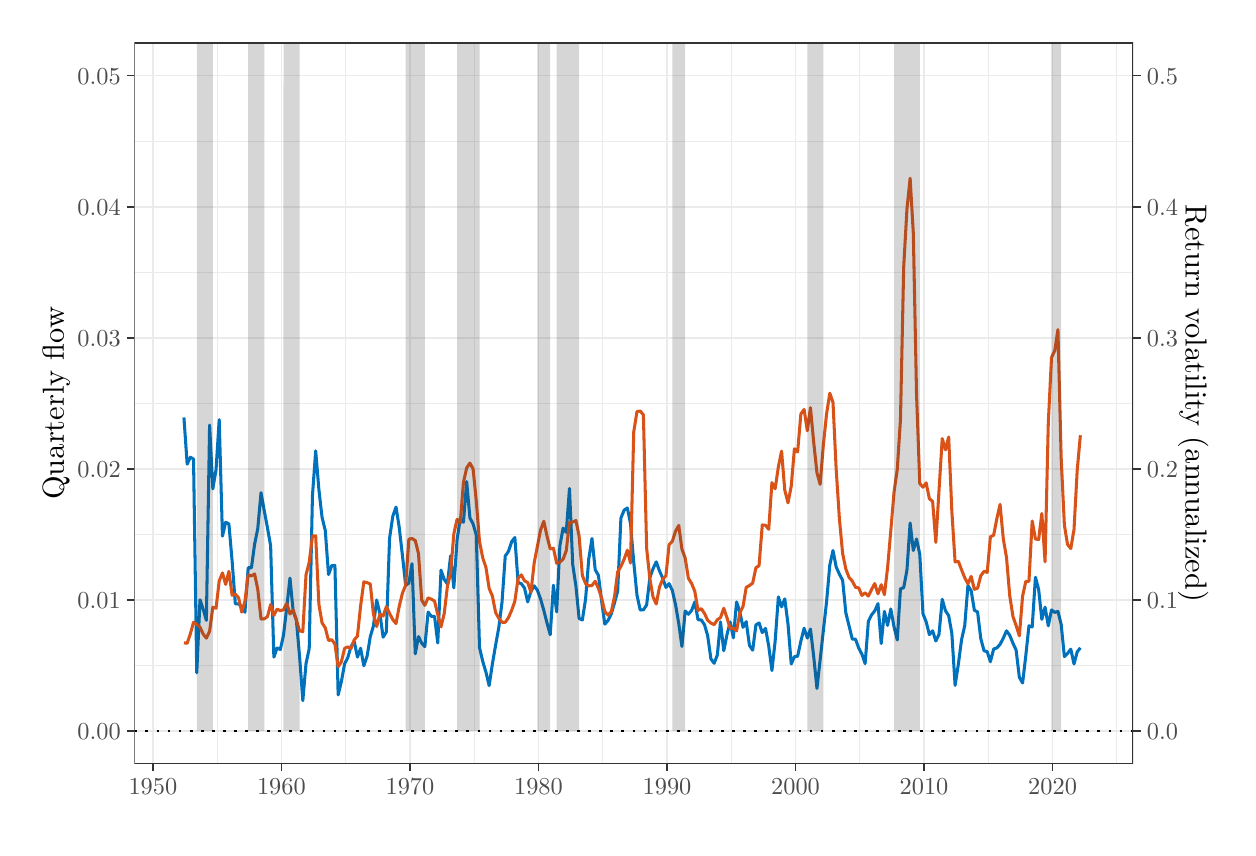
\begin{tikzpicture}[x=1pt,y=1pt]
\definecolor{fillColor}{RGB}{255,255,255}
\path[use as bounding box,fill=fillColor,fill opacity=0.00] (0,0) rectangle (433.62,289.08);
\begin{scope}
\path[clip] (  0.00,  0.00) rectangle (433.62,289.08);
\definecolor{drawColor}{RGB}{255,255,255}
\definecolor{fillColor}{RGB}{255,255,255}

\path[draw=drawColor,line width= 0.6pt,line join=round,line cap=round,fill=fillColor] (  0.00,  0.00) rectangle (433.62,289.08);
\end{scope}
\begin{scope}
\path[clip] ( 38.56, 23.11) rectangle (399.46,283.58);
\definecolor{fillColor}{RGB}{255,255,255}

\path[fill=fillColor] ( 38.56, 23.11) rectangle (399.46,283.58);
\definecolor{drawColor}{gray}{0.92}

\path[draw=drawColor,line width= 0.3pt,line join=round] ( 38.56, 58.63) --
	(399.46, 58.63);

\path[draw=drawColor,line width= 0.3pt,line join=round] ( 38.56,105.99) --
	(399.46,105.99);

\path[draw=drawColor,line width= 0.3pt,line join=round] ( 38.56,153.34) --
	(399.46,153.34);

\path[draw=drawColor,line width= 0.3pt,line join=round] ( 38.56,200.70) --
	(399.46,200.70);

\path[draw=drawColor,line width= 0.3pt,line join=round] ( 38.56,248.06) --
	(399.46,248.06);

\path[draw=drawColor,line width= 0.3pt,line join=round] ( 68.46, 23.11) --
	( 68.46,283.58);

\path[draw=drawColor,line width= 0.3pt,line join=round] (114.91, 23.11) --
	(114.91,283.58);

\path[draw=drawColor,line width= 0.3pt,line join=round] (161.35, 23.11) --
	(161.35,283.58);

\path[draw=drawColor,line width= 0.3pt,line join=round] (207.79, 23.11) --
	(207.79,283.58);

\path[draw=drawColor,line width= 0.3pt,line join=round] (254.24, 23.11) --
	(254.24,283.58);

\path[draw=drawColor,line width= 0.3pt,line join=round] (300.68, 23.11) --
	(300.68,283.58);

\path[draw=drawColor,line width= 0.3pt,line join=round] (347.13, 23.11) --
	(347.13,283.58);

\path[draw=drawColor,line width= 0.3pt,line join=round] (393.57, 23.11) --
	(393.57,283.58);

\path[draw=drawColor,line width= 0.6pt,line join=round] ( 38.56, 34.95) --
	(399.46, 34.95);

\path[draw=drawColor,line width= 0.6pt,line join=round] ( 38.56, 82.31) --
	(399.46, 82.31);

\path[draw=drawColor,line width= 0.6pt,line join=round] ( 38.56,129.67) --
	(399.46,129.67);

\path[draw=drawColor,line width= 0.6pt,line join=round] ( 38.56,177.02) --
	(399.46,177.02);

\path[draw=drawColor,line width= 0.6pt,line join=round] ( 38.56,224.38) --
	(399.46,224.38);

\path[draw=drawColor,line width= 0.6pt,line join=round] ( 38.56,271.74) --
	(399.46,271.74);

\path[draw=drawColor,line width= 0.6pt,line join=round] ( 45.24, 23.11) --
	( 45.24,283.58);

\path[draw=drawColor,line width= 0.6pt,line join=round] ( 91.68, 23.11) --
	( 91.68,283.58);

\path[draw=drawColor,line width= 0.6pt,line join=round] (138.13, 23.11) --
	(138.13,283.58);

\path[draw=drawColor,line width= 0.6pt,line join=round] (184.57, 23.11) --
	(184.57,283.58);

\path[draw=drawColor,line width= 0.6pt,line join=round] (231.02, 23.11) --
	(231.02,283.58);

\path[draw=drawColor,line width= 0.6pt,line join=round] (277.46, 23.11) --
	(277.46,283.58);

\path[draw=drawColor,line width= 0.6pt,line join=round] (323.91, 23.11) --
	(323.91,283.58);

\path[draw=drawColor,line width= 0.6pt,line join=round] (370.35, 23.11) --
	(370.35,283.58);
\definecolor{drawColor}{RGB}{0,114,189}

\path[draw=drawColor,line width= 1.1pt,line join=round] ( 56.46,148.23) --
	( 57.63,131.35) --
	( 58.78,133.87) --
	( 59.93,133.20) --
	( 61.10, 55.94) --
	( 62.27, 82.35) --
	( 63.43, 78.92) --
	( 64.57, 74.89) --
	( 65.74,145.46) --
	( 66.91,122.40) --
	( 68.07,129.42) --
	( 69.21,147.43) --
	( 70.38,105.35) --
	( 71.55,110.38) --
	( 72.71,109.76) --
	( 73.87, 96.40) --
	( 75.04, 80.86) --
	( 76.20, 80.88) --
	( 77.36, 79.88) --
	( 78.51, 77.82) --
	( 79.68, 93.93) --
	( 80.85, 93.90) --
	( 82.00,102.42) --
	( 83.15,108.14) --
	( 84.32,121.04) --
	( 85.49,114.52) --
	( 86.64,108.37) --
	( 87.79,101.91) --
	( 88.96, 61.63) --
	( 90.13, 64.95) --
	( 91.29, 64.36) --
	( 92.44, 69.56) --
	( 93.61, 79.49) --
	( 94.78, 90.18) --
	( 95.94, 78.14) --
	( 97.08, 75.12) --
	( 98.25, 61.92) --
	( 99.42, 45.90) --
	(100.58, 59.30) --
	(101.73, 64.67) --
	(102.90,119.95) --
	(104.07,136.18) --
	(105.22,122.28) --
	(106.37,112.15) --
	(107.54,107.36) --
	(108.71, 91.45) --
	(109.86, 94.67) --
	(111.02, 94.74) --
	(112.19, 47.96) --
	(113.36, 52.82) --
	(114.52, 59.22) --
	(115.66, 61.39) --
	(116.83, 65.47) --
	(118.00, 67.32) --
	(119.16, 61.64) --
	(120.30, 64.84) --
	(121.47, 58.49) --
	(122.64, 61.94) --
	(123.80, 68.99) --
	(124.94, 72.90) --
	(126.11, 82.27) --
	(127.28, 77.37) --
	(128.44, 68.83) --
	(129.60, 70.71) --
	(130.77,104.58) --
	(131.94,112.55) --
	(133.10,115.85) --
	(134.24,108.68) --
	(135.41, 98.46) --
	(136.58, 87.58) --
	(137.74, 88.39) --
	(138.88, 95.39) --
	(140.05, 62.80) --
	(141.22, 69.07) --
	(142.38, 66.67) --
	(143.52, 65.38) --
	(144.69, 77.91) --
	(145.86, 76.38) --
	(147.02, 76.35) --
	(148.18, 66.75) --
	(149.35, 93.06) --
	(150.52, 89.72) --
	(151.67, 88.05) --
	(152.82, 98.25) --
	(153.99, 86.66) --
	(155.16,104.07) --
	(156.31,111.69) --
	(157.46,110.35) --
	(158.63,125.07) --
	(159.80,111.97) --
	(160.96,109.72) --
	(162.10,105.75) --
	(163.27, 65.08) --
	(164.44, 60.06) --
	(165.60, 56.18) --
	(166.75, 51.32) --
	(167.92, 59.16) --
	(169.09, 65.97) --
	(170.25, 72.39) --
	(171.40, 81.43) --
	(172.57, 98.18) --
	(173.73, 99.82) --
	(174.89,103.34) --
	(176.04,104.86) --
	(177.21, 88.53) --
	(178.38, 88.19) --
	(179.53, 86.58) --
	(180.68, 81.58) --
	(181.85, 85.38) --
	(183.02, 87.39) --
	(184.17, 85.81) --
	(185.33, 82.66) --
	(186.50, 78.55) --
	(187.67, 73.90) --
	(188.83, 69.71) --
	(189.97, 87.62) --
	(191.14, 77.98) --
	(192.31,101.82) --
	(193.47,108.25) --
	(194.61,106.69) --
	(195.78,122.58) --
	(196.95, 95.08) --
	(198.11, 87.28) --
	(199.26, 75.61) --
	(200.43, 75.03) --
	(201.60, 82.62) --
	(202.75, 97.16) --
	(203.91,104.49) --
	(205.08, 93.21) --
	(206.25, 91.12) --
	(207.41, 81.73) --
	(208.55, 73.54) --
	(209.72, 74.87) --
	(210.89, 77.29) --
	(212.05, 81.20) --
	(213.19, 85.43) --
	(214.36,111.86) --
	(215.53,114.75) --
	(216.69,115.53) --
	(217.83,109.83) --
	(219.00, 95.94) --
	(220.17, 84.02) --
	(221.33, 78.66) --
	(222.49, 78.71) --
	(223.66, 80.48) --
	(224.83, 90.41) --
	(225.98, 93.59) --
	(227.13, 96.06) --
	(228.30, 92.78) --
	(229.47, 90.17) --
	(230.63, 86.82) --
	(231.77, 88.18) --
	(232.94, 85.72) --
	(234.11, 80.54) --
	(235.27, 73.75) --
	(236.41, 65.47) --
	(237.58, 78.29) --
	(238.75, 77.12) --
	(239.91, 78.51) --
	(241.06, 81.54) --
	(242.23, 75.15) --
	(243.40, 75.05) --
	(244.56, 73.36) --
	(245.71, 69.40) --
	(246.88, 61.00) --
	(248.05, 59.40) --
	(249.20, 62.36) --
	(250.35, 74.36) --
	(251.52, 63.92) --
	(252.69, 69.71) --
	(253.84, 74.34) --
	(254.99, 68.59) --
	(256.16, 81.58) --
	(257.33, 77.98) --
	(258.49, 72.40) --
	(259.64, 74.44) --
	(260.81, 65.85) --
	(261.98, 64.13) --
	(263.14, 73.26) --
	(264.28, 73.98) --
	(265.45, 70.49) --
	(266.62, 72.03) --
	(267.78, 65.60) --
	(268.93, 56.78) --
	(270.10, 67.42) --
	(271.26, 83.40) --
	(272.42, 79.82) --
	(273.57, 82.68) --
	(274.74, 73.61) --
	(275.91, 59.14) --
	(277.06, 61.79) --
	(278.22, 61.96) --
	(279.39, 67.39) --
	(280.56, 72.08) --
	(281.72, 68.52) --
	(282.86, 71.76) --
	(284.03, 61.85) --
	(285.20, 50.31) --
	(286.36, 60.66) --
	(287.50, 71.10) --
	(288.67, 81.53) --
	(289.84, 94.91) --
	(291.00,100.15) --
	(292.14, 94.25) --
	(293.31, 91.60) --
	(294.48, 89.41) --
	(295.64, 77.63) --
	(296.80, 72.95) --
	(297.97, 68.14) --
	(299.14, 68.10) --
	(300.30, 64.88) --
	(301.44, 62.72) --
	(302.61, 59.25) --
	(303.78, 74.55) --
	(304.94, 76.89) --
	(306.08, 78.32) --
	(307.25, 80.95) --
	(308.42, 66.52) --
	(309.58, 78.17) --
	(310.72, 73.09) --
	(311.89, 79.03) --
	(313.06, 72.53) --
	(314.22, 67.82) --
	(315.38, 86.32) --
	(316.55, 86.73) --
	(317.72, 93.05) --
	(318.87,110.10) --
	(320.02,100.16) --
	(321.19,104.32) --
	(322.36, 98.80) --
	(323.51, 77.33) --
	(324.66, 74.39) --
	(325.83, 69.74) --
	(327.00, 71.15) --
	(328.16, 67.46) --
	(329.30, 69.85) --
	(330.47, 82.54) --
	(331.64, 78.38) --
	(332.80, 76.60) --
	(333.95, 70.19) --
	(335.12, 51.40) --
	(336.29, 59.02) --
	(337.45, 67.88) --
	(338.60, 72.98) --
	(339.76, 87.52) --
	(340.93, 85.63) --
	(342.09, 78.53) --
	(343.24, 77.98) --
	(344.41, 68.27) --
	(345.58, 63.96) --
	(346.73, 63.57) --
	(347.88, 59.95) --
	(349.05, 64.56) --
	(350.22, 64.98) --
	(351.37, 66.23) --
	(352.53, 68.46) --
	(353.70, 71.13) --
	(354.87, 69.50) --
	(356.03, 66.65) --
	(357.17, 64.18) --
	(358.34, 54.32) --
	(359.51, 52.28) --
	(360.67, 62.19) --
	(361.81, 72.94) --
	(362.98, 72.51) --
	(364.15, 90.49) --
	(365.31, 86.11) --
	(366.46, 75.25) --
	(367.63, 79.68) --
	(368.80, 72.94) --
	(369.95, 78.69) --
	(371.11, 77.80) --
	(372.28, 78.14) --
	(373.45, 73.51) --
	(374.61, 61.79) --
	(375.75, 62.97) --
	(376.92, 64.51) --
	(378.09, 59.15) --
	(379.25, 63.53) --
	(380.39, 65.00);
\definecolor{drawColor}{RGB}{217,83,25}

\path[draw=drawColor,line width= 1.1pt,line join=round] ( 56.46, 66.79) --
	( 57.63, 66.63) --
	( 58.78, 70.01) --
	( 59.93, 74.24) --
	( 61.10, 73.46) --
	( 62.27, 72.45) --
	( 63.43, 69.92) --
	( 64.57, 68.49) --
	( 65.74, 70.98) --
	( 66.91, 79.67) --
	( 68.07, 79.29) --
	( 69.21, 89.14) --
	( 70.38, 92.05) --
	( 71.55, 87.89) --
	( 72.71, 92.64) --
	( 73.87, 84.00) --
	( 75.04, 84.38) --
	( 76.20, 83.09) --
	( 77.36, 77.90) --
	( 78.51, 81.82) --
	( 79.68, 91.35) --
	( 80.85, 90.96) --
	( 82.00, 91.70) --
	( 83.15, 86.06) --
	( 84.32, 75.39) --
	( 85.49, 75.45) --
	( 86.64, 76.25) --
	( 87.79, 80.63) --
	( 88.96, 76.66) --
	( 90.13, 78.98) --
	( 91.29, 78.40) --
	( 92.44, 78.75) --
	( 93.61, 81.06) --
	( 94.78, 77.21) --
	( 95.94, 78.67) --
	( 97.08, 74.98) --
	( 98.25, 71.08) --
	( 99.42, 70.85) --
	(100.58, 91.38) --
	(101.73, 95.84) --
	(102.90,105.40) --
	(104.07,105.47) --
	(105.22, 80.76) --
	(106.37, 74.04) --
	(107.54, 72.19) --
	(108.71, 67.64) --
	(109.86, 67.92) --
	(111.02, 66.37) --
	(112.19, 58.11) --
	(113.36, 59.95) --
	(114.52, 64.81) --
	(115.66, 65.33) --
	(116.83, 64.75) --
	(118.00, 67.89) --
	(119.16, 69.21) --
	(120.30, 80.08) --
	(121.47, 88.83) --
	(122.64, 88.53) --
	(123.80, 88.06) --
	(124.94, 77.14) --
	(126.11, 72.68) --
	(127.28, 77.15) --
	(128.44, 76.49) --
	(129.60, 79.88) --
	(130.77, 77.45) --
	(131.94, 75.16) --
	(133.10, 73.75) --
	(134.24, 79.88) --
	(135.41, 84.72) --
	(136.58, 87.65) --
	(137.74,104.26) --
	(138.88,104.48) --
	(140.05,103.77) --
	(141.22, 99.06) --
	(142.38, 82.25) --
	(143.52, 80.33) --
	(144.69, 83.03) --
	(145.86, 82.59) --
	(147.02, 81.88) --
	(148.18, 77.04) --
	(149.35, 72.54) --
	(150.52, 77.41) --
	(151.67, 87.21) --
	(152.82, 91.97) --
	(153.99,106.16) --
	(155.16,111.43) --
	(156.31,110.05) --
	(157.46,124.74) --
	(158.63,130.00) --
	(159.80,131.73) --
	(160.96,129.62) --
	(162.10,118.01) --
	(163.27,103.44) --
	(164.44, 97.48) --
	(165.60, 93.99) --
	(166.75, 86.47) --
	(167.92, 83.69) --
	(169.09, 77.73) --
	(170.25, 75.65) --
	(171.40, 74.24) --
	(172.57, 74.19) --
	(173.73, 75.89) --
	(174.89, 78.55) --
	(176.04, 81.81) --
	(177.21, 90.12) --
	(178.38, 91.36) --
	(179.53, 89.21) --
	(180.68, 88.59) --
	(181.85, 85.09) --
	(183.02, 95.64) --
	(184.17,101.64) --
	(185.33,107.56) --
	(186.50,110.74) --
	(187.67,105.31) --
	(188.83,100.72) --
	(189.97,100.99) --
	(191.14, 95.56) --
	(192.31, 95.98) --
	(193.47, 97.02) --
	(194.61,100.06) --
	(195.78,110.33) --
	(196.95,110.46) --
	(198.11,110.97) --
	(199.26,105.40) --
	(200.43, 91.12) --
	(201.60, 88.19) --
	(202.75, 87.35) --
	(203.91, 87.51) --
	(205.08, 89.04) --
	(206.25, 86.42) --
	(207.41, 82.96) --
	(208.55, 78.08) --
	(209.72, 76.80) --
	(210.89, 78.06) --
	(212.05, 83.47) --
	(213.19, 92.44) --
	(214.36, 94.36) --
	(215.53, 97.03) --
	(216.69,100.26) --
	(217.83, 95.62) --
	(219.00,143.01) --
	(220.17,150.37) --
	(221.33,150.55) --
	(222.49,149.16) --
	(223.66,100.92) --
	(224.83, 89.92) --
	(225.98, 83.33) --
	(227.13, 80.82) --
	(228.30, 86.93) --
	(229.47, 89.78) --
	(230.63, 91.01) --
	(231.77,102.25) --
	(232.94,103.50) --
	(234.11,107.13) --
	(235.27,109.20) --
	(236.41,100.63) --
	(237.58, 97.48) --
	(238.75, 90.11) --
	(239.91, 88.22) --
	(241.06, 85.41) --
	(242.23, 78.50) --
	(243.40, 79.15) --
	(244.56, 77.44) --
	(245.71, 74.96) --
	(246.88, 73.94) --
	(248.05, 73.35) --
	(249.20, 75.13) --
	(250.35, 75.89) --
	(251.52, 79.28) --
	(252.69, 75.87) --
	(253.84, 71.99) --
	(254.99, 72.13) --
	(256.16, 71.11) --
	(257.33, 77.64) --
	(258.49, 79.92) --
	(259.64, 86.85) --
	(260.81, 87.49) --
	(261.98, 88.38) --
	(263.14, 93.90) --
	(264.28, 94.67) --
	(265.45,109.38) --
	(266.62,109.28) --
	(267.78,107.81) --
	(268.93,124.69) --
	(270.10,122.46) --
	(271.26,130.41) --
	(272.42,136.06) --
	(273.57,121.99) --
	(274.74,117.36) --
	(275.91,123.39) --
	(277.06,136.92) --
	(278.22,135.75) --
	(279.39,149.50) --
	(280.56,151.12) --
	(281.72,143.42) --
	(282.86,151.77) --
	(284.03,139.22) --
	(285.20,128.25) --
	(286.36,124.05) --
	(287.50,138.10) --
	(288.67,149.44) --
	(289.84,156.99) --
	(291.00,153.66) --
	(292.14,129.69) --
	(293.31,111.68) --
	(294.48, 99.09) --
	(295.64, 93.48) --
	(296.80, 90.43) --
	(297.97, 89.10) --
	(299.14, 86.85) --
	(300.30, 86.64) --
	(301.44, 83.92) --
	(302.61, 84.86) --
	(303.78, 83.68) --
	(304.94, 86.08) --
	(306.08, 88.22) --
	(307.25, 84.50) --
	(308.42, 87.78) --
	(309.58, 84.18) --
	(310.72, 93.87) --
	(311.89,107.32) --
	(313.06,121.37) --
	(314.22,129.43) --
	(315.38,147.40) --
	(316.55,202.67) --
	(317.72,223.49) --
	(318.87,234.68) --
	(320.02,214.83) --
	(321.19,156.57) --
	(322.36,124.36) --
	(323.51,123.02) --
	(324.66,124.58) --
	(325.83,118.87) --
	(327.00,117.90) --
	(328.16,103.08) --
	(329.30,121.67) --
	(330.47,140.60) --
	(331.64,136.53) --
	(332.80,141.16) --
	(333.95,114.22) --
	(335.12, 96.02) --
	(336.29, 96.26) --
	(337.45, 93.20) --
	(338.60, 90.33) --
	(339.76, 88.12) --
	(340.93, 90.80) --
	(342.09, 86.12) --
	(343.24, 86.53) --
	(344.41, 91.01) --
	(345.58, 92.63) --
	(346.73, 92.25) --
	(347.88,105.13) --
	(349.05,105.65) --
	(350.22,111.74) --
	(351.37,116.80) --
	(352.53,104.47) --
	(353.70, 97.60) --
	(354.87, 83.78) --
	(356.03, 76.28) --
	(357.17, 73.03) --
	(358.34, 69.30) --
	(359.51, 83.68) --
	(360.67, 89.00) --
	(361.81, 89.02) --
	(362.98,110.84) --
	(364.15,104.33) --
	(365.31,104.12) --
	(366.46,113.54) --
	(367.63, 96.07) --
	(368.80,146.28) --
	(369.95,169.89) --
	(371.11,172.32) --
	(372.28,179.97) --
	(373.45,133.71) --
	(374.61,109.32) --
	(375.75,102.33) --
	(376.92,100.85) --
	(378.09,107.76) --
	(379.25,129.21) --
	(380.39,141.80);
\definecolor{fillColor}{RGB}{51,51,51}

\path[fill=fillColor,fill opacity=0.20] ( 55.29, 34.95) --
	( 55.61, 34.95) --
	( 56.13, 34.95) --
	( 56.46, 34.95) --
	( 56.78, 34.95) --
	( 57.30, 34.95) --
	( 57.63, 34.95) --
	( 57.95, 34.95) --
	( 58.46, 34.95) --
	( 58.78, 34.95) --
	( 59.11, 34.95) --
	( 59.60, 34.95) --
	( 59.93, 34.95) --
	( 60.26, 34.95) --
	( 60.77, 34.95) --
	( 61.10, 34.95) --
	( 61.10,2023.56) --
	( 66.90,2023.56) --
	( 66.91, 34.95) --
	( 67.24, 34.95) --
	( 67.74, 34.95) --
	( 68.07, 34.95) --
	( 68.39, 34.95) --
	( 68.88, 34.95) --
	( 69.21, 34.95) --
	( 69.54, 34.95) --
	( 70.05, 34.95) --
	( 70.38, 34.95) --
	( 70.71, 34.95) --
	( 71.22, 34.95) --
	( 71.55, 34.95) --
	( 71.88, 34.95) --
	( 72.38, 34.95) --
	( 72.71, 34.95) --
	( 73.04, 34.95) --
	( 73.54, 34.95) --
	( 73.87, 34.95) --
	( 74.19, 34.95) --
	( 74.71, 34.95) --
	( 75.04, 34.95) --
	( 75.36, 34.95) --
	( 75.88, 34.95) --
	( 76.20, 34.95) --
	( 76.53, 34.95) --
	( 77.03, 34.95) --
	( 77.36, 34.95) --
	( 77.69, 34.95) --
	( 78.18, 34.95) --
	( 78.51, 34.95) --
	( 78.83, 34.95) --
	( 79.35, 34.95) --
	( 79.68, 34.95) --
	( 79.68,2023.56) --
	( 85.48,2023.56) --
	( 85.49, 34.95) --
	( 85.81, 34.95) --
	( 86.32, 34.95) --
	( 86.64, 34.95) --
	( 86.97, 34.95) --
	( 87.46, 34.95) --
	( 87.79, 34.95) --
	( 88.12, 34.95) --
	( 88.63, 34.95) --
	( 88.96, 34.95) --
	( 89.29, 34.95) --
	( 89.80, 34.95) --
	( 90.13, 34.95) --
	( 90.46, 34.95) --
	( 90.96, 34.95) --
	( 91.29, 34.95) --
	( 91.61, 34.95) --
	( 92.12, 34.95) --
	( 92.44, 34.95) --
	( 92.45,2023.56) --
	( 98.25,2023.56) --
	( 98.25, 34.95) --
	( 98.58, 34.95) --
	( 99.10, 34.95) --
	( 99.42, 34.95) --
	( 99.75, 34.95) --
	(100.25, 34.95) --
	(100.58, 34.95) --
	(100.91, 34.95) --
	(101.40, 34.95) --
	(101.73, 34.95) --
	(102.05, 34.95) --
	(102.57, 34.95) --
	(102.90, 34.95) --
	(103.22, 34.95) --
	(103.74, 34.95) --
	(104.07, 34.95) --
	(104.39, 34.95) --
	(104.89, 34.95) --
	(105.22, 34.95) --
	(105.55, 34.95) --
	(106.04, 34.95) --
	(106.37, 34.95) --
	(106.69, 34.95) --
	(107.21, 34.95) --
	(107.54, 34.95) --
	(107.86, 34.95) --
	(108.38, 34.95) --
	(108.71, 34.95) --
	(109.03, 34.95) --
	(109.54, 34.95) --
	(109.86, 34.95) --
	(110.19, 34.95) --
	(110.69, 34.95) --
	(111.02, 34.95) --
	(111.35, 34.95) --
	(111.86, 34.95) --
	(112.19, 34.95) --
	(112.52, 34.95) --
	(113.03, 34.95) --
	(113.36, 34.95) --
	(113.69, 34.95) --
	(114.19, 34.95) --
	(114.52, 34.95) --
	(114.84, 34.95) --
	(115.33, 34.95) --
	(115.66, 34.95) --
	(115.99, 34.95) --
	(116.50, 34.95) --
	(116.83, 34.95) --
	(117.16, 34.95) --
	(117.67, 34.95) --
	(118.00, 34.95) --
	(118.33, 34.95) --
	(118.83, 34.95) --
	(119.16, 34.95) --
	(119.49, 34.95) --
	(119.98, 34.95) --
	(120.30, 34.95) --
	(120.63, 34.95) --
	(121.15, 34.95) --
	(121.47, 34.95) --
	(121.80, 34.95) --
	(122.32, 34.95) --
	(122.64, 34.95) --
	(122.97, 34.95) --
	(123.47, 34.95) --
	(123.80, 34.95) --
	(124.13, 34.95) --
	(124.62, 34.95) --
	(124.94, 34.95) --
	(125.27, 34.95) --
	(125.79, 34.95) --
	(126.11, 34.95) --
	(126.44, 34.95) --
	(126.96, 34.95) --
	(127.28, 34.95) --
	(127.61, 34.95) --
	(128.11, 34.95) --
	(128.44, 34.95) --
	(128.77, 34.95) --
	(129.27, 34.95) --
	(129.60, 34.95) --
	(129.93, 34.95) --
	(130.44, 34.95) --
	(130.77, 34.95) --
	(131.10, 34.95) --
	(131.61, 34.95) --
	(131.94, 34.95) --
	(132.27, 34.95) --
	(132.77, 34.95) --
	(133.10, 34.95) --
	(133.42, 34.95) --
	(133.91, 34.95) --
	(134.24, 34.95) --
	(134.57, 34.95) --
	(135.08, 34.95) --
	(135.41, 34.95) --
	(135.74, 34.95) --
	(136.25, 34.95) --
	(136.58, 34.95) --
	(136.58,2023.56) --
	(143.52,2023.56) --
	(143.52, 34.95) --
	(143.85, 34.95) --
	(144.36, 34.95) --
	(144.69, 34.95) --
	(145.02, 34.95) --
	(145.53, 34.95) --
	(145.86, 34.95) --
	(146.19, 34.95) --
	(146.69, 34.95) --
	(147.02, 34.95) --
	(147.35, 34.95) --
	(147.85, 34.95) --
	(148.18, 34.95) --
	(148.50, 34.95) --
	(149.02, 34.95) --
	(149.35, 34.95) --
	(149.67, 34.95) --
	(150.19, 34.95) --
	(150.52, 34.95) --
	(150.84, 34.95) --
	(151.35, 34.95) --
	(151.67, 34.95) --
	(152.00, 34.95) --
	(152.49, 34.95) --
	(152.82, 34.95) --
	(153.14, 34.95) --
	(153.66, 34.95) --
	(153.99, 34.95) --
	(154.31, 34.95) --
	(154.83, 34.95) --
	(155.16, 34.95) --
	(155.16,2023.56) --
	(163.26,2023.56) --
	(163.27, 34.95) --
	(163.60, 34.95) --
	(164.11, 34.95) --
	(164.44, 34.95) --
	(164.77, 34.95) --
	(165.27, 34.95) --
	(165.60, 34.95) --
	(165.92, 34.95) --
	(166.43, 34.95) --
	(166.75, 34.95) --
	(167.08, 34.95) --
	(167.60, 34.95) --
	(167.92, 34.95) --
	(168.25, 34.95) --
	(168.77, 34.95) --
	(169.09, 34.95) --
	(169.42, 34.95) --
	(169.92, 34.95) --
	(170.25, 34.95) --
	(170.58, 34.95) --
	(171.07, 34.95) --
	(171.40, 34.95) --
	(171.72, 34.95) --
	(172.24, 34.95) --
	(172.57, 34.95) --
	(172.89, 34.95) --
	(173.41, 34.95) --
	(173.73, 34.95) --
	(174.06, 34.95) --
	(174.56, 34.95) --
	(174.89, 34.95) --
	(175.22, 34.95) --
	(175.71, 34.95) --
	(176.04, 34.95) --
	(176.36, 34.95) --
	(176.88, 34.95) --
	(177.21, 34.95) --
	(177.53, 34.95) --
	(178.05, 34.95) --
	(178.38, 34.95) --
	(178.70, 34.95) --
	(179.21, 34.95) --
	(179.53, 34.95) --
	(179.86, 34.95) --
	(180.35, 34.95) --
	(180.68, 34.95) --
	(181.01, 34.95) --
	(181.52, 34.95) --
	(181.85, 34.95) --
	(182.18, 34.95) --
	(182.69, 34.95) --
	(183.02, 34.95) --
	(183.34, 34.95) --
	(183.85, 34.95) --
	(184.17, 34.95) --
	(184.18,2023.56) --
	(188.82,2023.56) --
	(188.83, 34.95) --
	(189.16, 34.95) --
	(189.65, 34.95) --
	(189.97, 34.95) --
	(190.30, 34.95) --
	(190.82, 34.95) --
	(191.14, 34.95) --
	(191.15,2023.56) --
	(199.25,2023.56) --
	(199.26, 34.95) --
	(199.58, 34.95) --
	(200.10, 34.95) --
	(200.43, 34.95) --
	(200.75, 34.95) --
	(201.27, 34.95) --
	(201.60, 34.95) --
	(201.92, 34.95) --
	(202.42, 34.95) --
	(202.75, 34.95) --
	(203.08, 34.95) --
	(203.58, 34.95) --
	(203.91, 34.95) --
	(204.24, 34.95) --
	(204.75, 34.95) --
	(205.08, 34.95) --
	(205.41, 34.95) --
	(205.92, 34.95) --
	(206.25, 34.95) --
	(206.58, 34.95) --
	(207.08, 34.95) --
	(207.41, 34.95) --
	(207.73, 34.95) --
	(208.22, 34.95) --
	(208.55, 34.95) --
	(208.88, 34.95) --
	(209.39, 34.95) --
	(209.72, 34.95) --
	(210.05, 34.95) --
	(210.56, 34.95) --
	(210.89, 34.95) --
	(211.22, 34.95) --
	(211.72, 34.95) --
	(212.05, 34.95) --
	(212.38, 34.95) --
	(212.86, 34.95) --
	(213.19, 34.95) --
	(213.52, 34.95) --
	(214.03, 34.95) --
	(214.36, 34.95) --
	(214.69, 34.95) --
	(215.20, 34.95) --
	(215.53, 34.95) --
	(215.86, 34.95) --
	(216.36, 34.95) --
	(216.69, 34.95) --
	(217.02, 34.95) --
	(217.51, 34.95) --
	(217.83, 34.95) --
	(218.16, 34.95) --
	(218.68, 34.95) --
	(219.00, 34.95) --
	(219.33, 34.95) --
	(219.85, 34.95) --
	(220.17, 34.95) --
	(220.50, 34.95) --
	(221.00, 34.95) --
	(221.33, 34.95) --
	(221.66, 34.95) --
	(222.16, 34.95) --
	(222.49, 34.95) --
	(222.81, 34.95) --
	(223.33, 34.95) --
	(223.66, 34.95) --
	(223.98, 34.95) --
	(224.50, 34.95) --
	(224.83, 34.95) --
	(225.15, 34.95) --
	(225.66, 34.95) --
	(225.98, 34.95) --
	(226.31, 34.95) --
	(226.80, 34.95) --
	(227.13, 34.95) --
	(227.46, 34.95) --
	(227.97, 34.95) --
	(228.30, 34.95) --
	(228.63, 34.95) --
	(229.14, 34.95) --
	(229.47, 34.95) --
	(229.80, 34.95) --
	(230.30, 34.95) --
	(230.63, 34.95) --
	(230.95, 34.95) --
	(231.44, 34.95) --
	(231.77, 34.95) --
	(232.10, 34.95) --
	(232.61, 34.95) --
	(232.94, 34.95) --
	(232.94,2023.56) --
	(237.58,2023.56) --
	(237.58, 34.95) --
	(237.91, 34.95) --
	(238.42, 34.95) --
	(238.75, 34.95) --
	(239.08, 34.95) --
	(239.58, 34.95) --
	(239.91, 34.95) --
	(240.24, 34.95) --
	(240.74, 34.95) --
	(241.06, 34.95) --
	(241.39, 34.95) --
	(241.91, 34.95) --
	(242.23, 34.95) --
	(242.56, 34.95) --
	(243.08, 34.95) --
	(243.40, 34.95) --
	(243.73, 34.95) --
	(244.23, 34.95) --
	(244.56, 34.95) --
	(244.89, 34.95) --
	(245.38, 34.95) --
	(245.71, 34.95) --
	(246.03, 34.95) --
	(246.55, 34.95) --
	(246.88, 34.95) --
	(247.20, 34.95) --
	(247.72, 34.95) --
	(248.05, 34.95) --
	(248.37, 34.95) --
	(248.88, 34.95) --
	(249.20, 34.95) --
	(249.53, 34.95) --
	(250.02, 34.95) --
	(250.35, 34.95) --
	(250.67, 34.95) --
	(251.19, 34.95) --
	(251.52, 34.95) --
	(251.84, 34.95) --
	(252.36, 34.95) --
	(252.69, 34.95) --
	(253.01, 34.95) --
	(253.52, 34.95) --
	(253.84, 34.95) --
	(254.17, 34.95) --
	(254.66, 34.95) --
	(254.99, 34.95) --
	(255.32, 34.95) --
	(255.83, 34.95) --
	(256.16, 34.95) --
	(256.49, 34.95) --
	(257.00, 34.95) --
	(257.33, 34.95) --
	(257.66, 34.95) --
	(258.16, 34.95) --
	(258.49, 34.95) --
	(258.81, 34.95) --
	(259.32, 34.95) --
	(259.64, 34.95) --
	(259.97, 34.95) --
	(260.49, 34.95) --
	(260.81, 34.95) --
	(261.14, 34.95) --
	(261.66, 34.95) --
	(261.98, 34.95) --
	(262.31, 34.95) --
	(262.81, 34.95) --
	(263.14, 34.95) --
	(263.47, 34.95) --
	(263.96, 34.95) --
	(264.28, 34.95) --
	(264.61, 34.95) --
	(265.13, 34.95) --
	(265.45, 34.95) --
	(265.78, 34.95) --
	(266.30, 34.95) --
	(266.62, 34.95) --
	(266.95, 34.95) --
	(267.45, 34.95) --
	(267.78, 34.95) --
	(268.11, 34.95) --
	(268.60, 34.95) --
	(268.93, 34.95) --
	(269.25, 34.95) --
	(269.77, 34.95) --
	(270.10, 34.95) --
	(270.42, 34.95) --
	(270.94, 34.95) --
	(271.26, 34.95) --
	(271.59, 34.95) --
	(272.09, 34.95) --
	(272.42, 34.95) --
	(272.75, 34.95) --
	(273.24, 34.95) --
	(273.57, 34.95) --
	(273.89, 34.95) --
	(274.41, 34.95) --
	(274.74, 34.95) --
	(275.06, 34.95) --
	(275.58, 34.95) --
	(275.91, 34.95) --
	(276.23, 34.95) --
	(276.74, 34.95) --
	(277.06, 34.95) --
	(277.39, 34.95) --
	(277.89, 34.95) --
	(278.22, 34.95) --
	(278.55, 34.95) --
	(279.06, 34.95) --
	(279.39, 34.95) --
	(279.72, 34.95) --
	(280.23, 34.95) --
	(280.56, 34.95) --
	(280.89, 34.95) --
	(281.39, 34.95) --
	(281.72, 34.95) --
	(281.72,2023.56) --
	(287.50,2023.56) --
	(287.50, 34.95) --
	(287.83, 34.95) --
	(288.35, 34.95) --
	(288.67, 34.95) --
	(289.00, 34.95) --
	(289.52, 34.95) --
	(289.84, 34.95) --
	(290.17, 34.95) --
	(290.67, 34.95) --
	(291.00, 34.95) --
	(291.33, 34.95) --
	(291.82, 34.95) --
	(292.14, 34.95) --
	(292.47, 34.95) --
	(292.99, 34.95) --
	(293.31, 34.95) --
	(293.64, 34.95) --
	(294.16, 34.95) --
	(294.48, 34.95) --
	(294.81, 34.95) --
	(295.31, 34.95) --
	(295.64, 34.95) --
	(295.97, 34.95) --
	(296.47, 34.95) --
	(296.80, 34.95) --
	(297.13, 34.95) --
	(297.64, 34.95) --
	(297.97, 34.95) --
	(298.30, 34.95) --
	(298.81, 34.95) --
	(299.14, 34.95) --
	(299.47, 34.95) --
	(299.97, 34.95) --
	(300.30, 34.95) --
	(300.62, 34.95) --
	(301.11, 34.95) --
	(301.44, 34.95) --
	(301.77, 34.95) --
	(302.28, 34.95) --
	(302.61, 34.95) --
	(302.94, 34.95) --
	(303.45, 34.95) --
	(303.78, 34.95) --
	(304.11, 34.95) --
	(304.61, 34.95) --
	(304.94, 34.95) --
	(305.26, 34.95) --
	(305.75, 34.95) --
	(306.08, 34.95) --
	(306.41, 34.95) --
	(306.92, 34.95) --
	(307.25, 34.95) --
	(307.58, 34.95) --
	(308.09, 34.95) --
	(308.42, 34.95) --
	(308.75, 34.95) --
	(309.25, 34.95) --
	(309.58, 34.95) --
	(309.91, 34.95) --
	(310.39, 34.95) --
	(310.72, 34.95) --
	(311.05, 34.95) --
	(311.56, 34.95) --
	(311.89, 34.95) --
	(312.22, 34.95) --
	(312.73, 34.95) --
	(313.06, 34.95) --
	(313.07,2023.56) --
	(322.35,2023.56) --
	(322.36, 34.95) --
	(322.68, 34.95) --
	(323.19, 34.95) --
	(323.51, 34.95) --
	(323.84, 34.95) --
	(324.33, 34.95) --
	(324.66, 34.95) --
	(324.99, 34.95) --
	(325.50, 34.95) --
	(325.83, 34.95) --
	(326.16, 34.95) --
	(326.67, 34.95) --
	(327.00, 34.95) --
	(327.33, 34.95) --
	(327.83, 34.95) --
	(328.16, 34.95) --
	(328.48, 34.95) --
	(328.97, 34.95) --
	(329.30, 34.95) --
	(329.63, 34.95) --
	(330.14, 34.95) --
	(330.47, 34.95) --
	(330.80, 34.95) --
	(331.31, 34.95) --
	(331.64, 34.95) --
	(331.97, 34.95) --
	(332.47, 34.95) --
	(332.80, 34.95) --
	(333.12, 34.95) --
	(333.63, 34.95) --
	(333.95, 34.95) --
	(334.28, 34.95) --
	(334.80, 34.95) --
	(335.12, 34.95) --
	(335.45, 34.95) --
	(335.97, 34.95) --
	(336.29, 34.95) --
	(336.62, 34.95) --
	(337.12, 34.95) --
	(337.45, 34.95) --
	(337.78, 34.95) --
	(338.27, 34.95) --
	(338.60, 34.95) --
	(338.92, 34.95) --
	(339.44, 34.95) --
	(339.76, 34.95) --
	(340.09, 34.95) --
	(340.61, 34.95) --
	(340.93, 34.95) --
	(341.26, 34.95) --
	(341.76, 34.95) --
	(342.09, 34.95) --
	(342.42, 34.95) --
	(342.91, 34.95) --
	(343.24, 34.95) --
	(343.56, 34.95) --
	(344.08, 34.95) --
	(344.41, 34.95) --
	(344.73, 34.95) --
	(345.25, 34.95) --
	(345.58, 34.95) --
	(345.90, 34.95) --
	(346.41, 34.95) --
	(346.73, 34.95) --
	(347.06, 34.95) --
	(347.55, 34.95) --
	(347.88, 34.95) --
	(348.21, 34.95) --
	(348.72, 34.95) --
	(349.05, 34.95) --
	(349.37, 34.95) --
	(349.89, 34.95) --
	(350.22, 34.95) --
	(350.54, 34.95) --
	(351.05, 34.95) --
	(351.37, 34.95) --
	(351.70, 34.95) --
	(352.20, 34.95) --
	(352.53, 34.95) --
	(352.86, 34.95) --
	(353.37, 34.95) --
	(353.70, 34.95) --
	(354.03, 34.95) --
	(354.54, 34.95) --
	(354.87, 34.95) --
	(355.20, 34.95) --
	(355.70, 34.95) --
	(356.03, 34.95) --
	(356.36, 34.95) --
	(356.85, 34.95) --
	(357.17, 34.95) --
	(357.50, 34.95) --
	(358.02, 34.95) --
	(358.34, 34.95) --
	(358.67, 34.95) --
	(359.19, 34.95) --
	(359.51, 34.95) --
	(359.84, 34.95) --
	(360.34, 34.95) --
	(360.67, 34.95) --
	(361.00, 34.95) --
	(361.49, 34.95) --
	(361.81, 34.95) --
	(362.14, 34.95) --
	(362.66, 34.95) --
	(362.98, 34.95) --
	(363.31, 34.95) --
	(363.83, 34.95) --
	(364.15, 34.95) --
	(364.48, 34.95) --
	(364.98, 34.95) --
	(365.31, 34.95) --
	(365.64, 34.95) --
	(366.13, 34.95) --
	(366.46, 34.95) --
	(366.78, 34.95) --
	(367.30, 34.95) --
	(367.63, 34.95) --
	(367.95, 34.95) --
	(368.47, 34.95) --
	(368.80, 34.95) --
	(369.12, 34.95) --
	(369.62, 34.95) --
	(369.95, 34.95) --
	(369.96,2023.56) --
	(373.44,2023.56) --
	(373.45, 34.95) --
	(373.78, 34.95) --
	(374.28, 34.95) --
	(374.61, 34.95) --
	(374.93, 34.95) --
	(375.42, 34.95) --
	(375.75, 34.95) --
	(376.08, 34.95) --
	(376.59, 34.95) --
	(376.92, 34.95) --
	(377.25, 34.95) --
	(377.76, 34.95) --
	(378.09, 34.95) --
	(378.42, 34.95) --
	(378.92, 34.95) --
	(379.25, 34.95) --
	(379.57, 34.95) --
	(380.06, 34.95) --
	(380.39, 34.95) --
	(380.72, 34.95) --
	(381.23, 34.95) --
	(381.56, 34.95) --
	(381.89, 34.95) --
	(382.40, 34.95) --
	(382.73, 34.95) --
	(383.06, 34.95) --
	(382.73, 34.95) --
	(382.40, 34.95) --
	(381.89, 34.95) --
	(381.56, 34.95) --
	(381.23, 34.95) --
	(380.72, 34.95) --
	(380.39, 34.95) --
	(380.06, 34.95) --
	(379.57, 34.95) --
	(379.25, 34.95) --
	(378.92, 34.95) --
	(378.42, 34.95) --
	(378.09, 34.95) --
	(377.76, 34.95) --
	(377.25, 34.95) --
	(376.92, 34.95) --
	(376.59, 34.95) --
	(376.08, 34.95) --
	(375.75, 34.95) --
	(375.42, 34.95) --
	(374.93, 34.95) --
	(374.61, 34.95) --
	(374.28, 34.95) --
	(373.78, 34.95) --
	(373.45, 34.95) --
	(373.12, 34.95) --
	(372.61, 34.95) --
	(372.28, 34.95) --
	(371.95, 34.95) --
	(371.44, 34.95) --
	(371.11, 34.95) --
	(370.78, 34.95) --
	(370.28, 34.95) --
	(369.95, 34.95) --
	(369.62, 34.95) --
	(369.12, 34.95) --
	(368.80, 34.95) --
	(368.47, 34.95) --
	(367.95, 34.95) --
	(367.63, 34.95) --
	(367.30, 34.95) --
	(366.78, 34.95) --
	(366.46, 34.95) --
	(366.13, 34.95) --
	(365.64, 34.95) --
	(365.31, 34.95) --
	(364.98, 34.95) --
	(364.48, 34.95) --
	(364.15, 34.95) --
	(363.83, 34.95) --
	(363.31, 34.95) --
	(362.98, 34.95) --
	(362.66, 34.95) --
	(362.14, 34.95) --
	(361.81, 34.95) --
	(361.49, 34.95) --
	(361.00, 34.95) --
	(360.67, 34.95) --
	(360.34, 34.95) --
	(359.84, 34.95) --
	(359.51, 34.95) --
	(359.19, 34.95) --
	(358.67, 34.95) --
	(358.34, 34.95) --
	(358.02, 34.95) --
	(357.50, 34.95) --
	(357.17, 34.95) --
	(356.85, 34.95) --
	(356.36, 34.95) --
	(356.03, 34.95) --
	(355.70, 34.95) --
	(355.20, 34.95) --
	(354.87, 34.95) --
	(354.54, 34.95) --
	(354.03, 34.95) --
	(353.70, 34.95) --
	(353.37, 34.95) --
	(352.86, 34.95) --
	(352.53, 34.95) --
	(352.20, 34.95) --
	(351.70, 34.95) --
	(351.37, 34.95) --
	(351.05, 34.95) --
	(350.54, 34.95) --
	(350.22, 34.95) --
	(349.89, 34.95) --
	(349.37, 34.95) --
	(349.05, 34.95) --
	(348.72, 34.95) --
	(348.21, 34.95) --
	(347.88, 34.95) --
	(347.55, 34.95) --
	(347.06, 34.95) --
	(346.73, 34.95) --
	(346.41, 34.95) --
	(345.90, 34.95) --
	(345.58, 34.95) --
	(345.25, 34.95) --
	(344.73, 34.95) --
	(344.41, 34.95) --
	(344.08, 34.95) --
	(343.56, 34.95) --
	(343.24, 34.95) --
	(342.91, 34.95) --
	(342.42, 34.95) --
	(342.09, 34.95) --
	(341.76, 34.95) --
	(341.26, 34.95) --
	(340.93, 34.95) --
	(340.61, 34.95) --
	(340.09, 34.95) --
	(339.76, 34.95) --
	(339.44, 34.95) --
	(338.92, 34.95) --
	(338.60, 34.95) --
	(338.27, 34.95) --
	(337.78, 34.95) --
	(337.45, 34.95) --
	(337.12, 34.95) --
	(336.62, 34.95) --
	(336.29, 34.95) --
	(335.97, 34.95) --
	(335.45, 34.95) --
	(335.12, 34.95) --
	(334.80, 34.95) --
	(334.28, 34.95) --
	(333.95, 34.95) --
	(333.63, 34.95) --
	(333.12, 34.95) --
	(332.80, 34.95) --
	(332.47, 34.95) --
	(331.97, 34.95) --
	(331.64, 34.95) --
	(331.31, 34.95) --
	(330.80, 34.95) --
	(330.47, 34.95) --
	(330.14, 34.95) --
	(329.63, 34.95) --
	(329.30, 34.95) --
	(328.97, 34.95) --
	(328.48, 34.95) --
	(328.16, 34.95) --
	(327.83, 34.95) --
	(327.33, 34.95) --
	(327.00, 34.95) --
	(326.67, 34.95) --
	(326.16, 34.95) --
	(325.83, 34.95) --
	(325.50, 34.95) --
	(324.99, 34.95) --
	(324.66, 34.95) --
	(324.33, 34.95) --
	(323.84, 34.95) --
	(323.51, 34.95) --
	(323.19, 34.95) --
	(322.68, 34.95) --
	(322.36, 34.95) --
	(322.03, 34.95) --
	(321.51, 34.95) --
	(321.19, 34.95) --
	(320.86, 34.95) --
	(320.34, 34.95) --
	(320.02, 34.95) --
	(319.69, 34.95) --
	(319.20, 34.95) --
	(318.87, 34.95) --
	(318.55, 34.95) --
	(318.04, 34.95) --
	(317.72, 34.95) --
	(317.39, 34.95) --
	(316.87, 34.95) --
	(316.55, 34.95) --
	(316.22, 34.95) --
	(315.70, 34.95) --
	(315.38, 34.95) --
	(315.05, 34.95) --
	(314.55, 34.95) --
	(314.22, 34.95) --
	(313.89, 34.95) --
	(313.39, 34.95) --
	(313.06, 34.95) --
	(312.73, 34.95) --
	(312.22, 34.95) --
	(311.89, 34.95) --
	(311.56, 34.95) --
	(311.05, 34.95) --
	(310.72, 34.95) --
	(310.39, 34.95) --
	(309.91, 34.95) --
	(309.58, 34.95) --
	(309.25, 34.95) --
	(308.75, 34.95) --
	(308.42, 34.95) --
	(308.09, 34.95) --
	(307.58, 34.95) --
	(307.25, 34.95) --
	(306.92, 34.95) --
	(306.41, 34.95) --
	(306.08, 34.95) --
	(305.75, 34.95) --
	(305.26, 34.95) --
	(304.94, 34.95) --
	(304.61, 34.95) --
	(304.11, 34.95) --
	(303.78, 34.95) --
	(303.45, 34.95) --
	(302.94, 34.95) --
	(302.61, 34.95) --
	(302.28, 34.95) --
	(301.77, 34.95) --
	(301.44, 34.95) --
	(301.11, 34.95) --
	(300.62, 34.95) --
	(300.30, 34.95) --
	(299.97, 34.95) --
	(299.47, 34.95) --
	(299.14, 34.95) --
	(298.81, 34.95) --
	(298.30, 34.95) --
	(297.97, 34.95) --
	(297.64, 34.95) --
	(297.13, 34.95) --
	(296.80, 34.95) --
	(296.47, 34.95) --
	(295.97, 34.95) --
	(295.64, 34.95) --
	(295.31, 34.95) --
	(294.81, 34.95) --
	(294.48, 34.95) --
	(294.16, 34.95) --
	(293.64, 34.95) --
	(293.31, 34.95) --
	(292.99, 34.95) --
	(292.47, 34.95) --
	(292.14, 34.95) --
	(291.82, 34.95) --
	(291.33, 34.95) --
	(291.00, 34.95) --
	(290.67, 34.95) --
	(290.17, 34.95) --
	(289.84, 34.95) --
	(289.52, 34.95) --
	(289.00, 34.95) --
	(288.67, 34.95) --
	(288.35, 34.95) --
	(287.83, 34.95) --
	(287.50, 34.95) --
	(287.18, 34.95) --
	(286.69, 34.95) --
	(286.36, 34.95) --
	(286.03, 34.95) --
	(285.53, 34.95) --
	(285.20, 34.95) --
	(284.87, 34.95) --
	(284.36, 34.95) --
	(284.03, 34.95) --
	(283.70, 34.95) --
	(283.19, 34.95) --
	(282.86, 34.95) --
	(282.53, 34.95) --
	(282.04, 34.95) --
	(281.72, 34.95) --
	(281.39, 34.95) --
	(280.89, 34.95) --
	(280.56, 34.95) --
	(280.23, 34.95) --
	(279.72, 34.95) --
	(279.39, 34.95) --
	(279.06, 34.95) --
	(278.55, 34.95) --
	(278.22, 34.95) --
	(277.89, 34.95) --
	(277.39, 34.95) --
	(277.06, 34.95) --
	(276.74, 34.95) --
	(276.23, 34.95) --
	(275.91, 34.95) --
	(275.58, 34.95) --
	(275.06, 34.95) --
	(274.74, 34.95) --
	(274.41, 34.95) --
	(273.89, 34.95) --
	(273.57, 34.95) --
	(273.24, 34.95) --
	(272.75, 34.95) --
	(272.42, 34.95) --
	(272.09, 34.95) --
	(271.59, 34.95) --
	(271.26, 34.95) --
	(270.94, 34.95) --
	(270.42, 34.95) --
	(270.10, 34.95) --
	(269.77, 34.95) --
	(269.25, 34.95) --
	(268.93, 34.95) --
	(268.60, 34.95) --
	(268.11, 34.95) --
	(267.78, 34.95) --
	(267.45, 34.95) --
	(266.95, 34.95) --
	(266.62, 34.95) --
	(266.30, 34.95) --
	(265.78, 34.95) --
	(265.45, 34.95) --
	(265.13, 34.95) --
	(264.61, 34.95) --
	(264.28, 34.95) --
	(263.96, 34.95) --
	(263.47, 34.95) --
	(263.14, 34.95) --
	(262.81, 34.95) --
	(262.31, 34.95) --
	(261.98, 34.95) --
	(261.66, 34.95) --
	(261.14, 34.95) --
	(260.81, 34.95) --
	(260.49, 34.95) --
	(259.97, 34.95) --
	(259.64, 34.95) --
	(259.32, 34.95) --
	(258.81, 34.95) --
	(258.49, 34.95) --
	(258.16, 34.95) --
	(257.66, 34.95) --
	(257.33, 34.95) --
	(257.00, 34.95) --
	(256.49, 34.95) --
	(256.16, 34.95) --
	(255.83, 34.95) --
	(255.32, 34.95) --
	(254.99, 34.95) --
	(254.66, 34.95) --
	(254.17, 34.95) --
	(253.84, 34.95) --
	(253.52, 34.95) --
	(253.01, 34.95) --
	(252.69, 34.95) --
	(252.36, 34.95) --
	(251.84, 34.95) --
	(251.52, 34.95) --
	(251.19, 34.95) --
	(250.67, 34.95) --
	(250.35, 34.95) --
	(250.02, 34.95) --
	(249.53, 34.95) --
	(249.20, 34.95) --
	(248.88, 34.95) --
	(248.37, 34.95) --
	(248.05, 34.95) --
	(247.72, 34.95) --
	(247.20, 34.95) --
	(246.88, 34.95) --
	(246.55, 34.95) --
	(246.03, 34.95) --
	(245.71, 34.95) --
	(245.38, 34.95) --
	(244.89, 34.95) --
	(244.56, 34.95) --
	(244.23, 34.95) --
	(243.73, 34.95) --
	(243.40, 34.95) --
	(243.08, 34.95) --
	(242.56, 34.95) --
	(242.23, 34.95) --
	(241.91, 34.95) --
	(241.39, 34.95) --
	(241.06, 34.95) --
	(240.74, 34.95) --
	(240.24, 34.95) --
	(239.91, 34.95) --
	(239.58, 34.95) --
	(239.08, 34.95) --
	(238.75, 34.95) --
	(238.42, 34.95) --
	(237.91, 34.95) --
	(237.58, 34.95) --
	(237.25, 34.95) --
	(236.74, 34.95) --
	(236.41, 34.95) --
	(236.08, 34.95) --
	(235.59, 34.95) --
	(235.27, 34.95) --
	(234.94, 34.95) --
	(234.44, 34.95) --
	(234.11, 34.95) --
	(233.78, 34.95) --
	(233.27, 34.95) --
	(232.94, 34.95) --
	(232.61, 34.95) --
	(232.10, 34.95) --
	(231.77, 34.95) --
	(231.44, 34.95) --
	(230.95, 34.95) --
	(230.63, 34.95) --
	(230.30, 34.95) --
	(229.80, 34.95) --
	(229.47, 34.95) --
	(229.14, 34.95) --
	(228.63, 34.95) --
	(228.30, 34.95) --
	(227.97, 34.95) --
	(227.46, 34.95) --
	(227.13, 34.95) --
	(226.80, 34.95) --
	(226.31, 34.95) --
	(225.98, 34.95) --
	(225.66, 34.95) --
	(225.15, 34.95) --
	(224.83, 34.95) --
	(224.50, 34.95) --
	(223.98, 34.95) --
	(223.66, 34.95) --
	(223.33, 34.95) --
	(222.81, 34.95) --
	(222.49, 34.95) --
	(222.16, 34.95) --
	(221.66, 34.95) --
	(221.33, 34.95) --
	(221.00, 34.95) --
	(220.50, 34.95) --
	(220.17, 34.95) --
	(219.85, 34.95) --
	(219.33, 34.95) --
	(219.00, 34.95) --
	(218.68, 34.95) --
	(218.16, 34.95) --
	(217.83, 34.95) --
	(217.51, 34.95) --
	(217.02, 34.95) --
	(216.69, 34.95) --
	(216.36, 34.95) --
	(215.86, 34.95) --
	(215.53, 34.95) --
	(215.20, 34.95) --
	(214.69, 34.95) --
	(214.36, 34.95) --
	(214.03, 34.95) --
	(213.52, 34.95) --
	(213.19, 34.95) --
	(212.86, 34.95) --
	(212.38, 34.95) --
	(212.05, 34.95) --
	(211.72, 34.95) --
	(211.22, 34.95) --
	(210.89, 34.95) --
	(210.56, 34.95) --
	(210.05, 34.95) --
	(209.72, 34.95) --
	(209.39, 34.95) --
	(208.88, 34.95) --
	(208.55, 34.95) --
	(208.22, 34.95) --
	(207.73, 34.95) --
	(207.41, 34.95) --
	(207.08, 34.95) --
	(206.58, 34.95) --
	(206.25, 34.95) --
	(205.92, 34.95) --
	(205.41, 34.95) --
	(205.08, 34.95) --
	(204.75, 34.95) --
	(204.24, 34.95) --
	(203.91, 34.95) --
	(203.58, 34.95) --
	(203.08, 34.95) --
	(202.75, 34.95) --
	(202.42, 34.95) --
	(201.92, 34.95) --
	(201.60, 34.95) --
	(201.27, 34.95) --
	(200.75, 34.95) --
	(200.43, 34.95) --
	(200.10, 34.95) --
	(199.58, 34.95) --
	(199.26, 34.95) --
	(198.93, 34.95) --
	(198.44, 34.95) --
	(198.11, 34.95) --
	(197.78, 34.95) --
	(197.28, 34.95) --
	(196.95, 34.95) --
	(196.63, 34.95) --
	(196.11, 34.95) --
	(195.78, 34.95) --
	(195.46, 34.95) --
	(194.94, 34.95) --
	(194.61, 34.95) --
	(194.29, 34.95) --
	(193.80, 34.95) --
	(193.47, 34.95) --
	(193.14, 34.95) --
	(192.64, 34.95) --
	(192.31, 34.95) --
	(191.99, 34.95) --
	(191.47, 34.95) --
	(191.14, 34.95) --
	(190.82, 34.95) --
	(190.30, 34.95) --
	(189.97, 34.95) --
	(189.65, 34.95) --
	(189.16, 34.95) --
	(188.83, 34.95) --
	(188.50, 34.95) --
	(188.00, 34.95) --
	(187.67, 34.95) --
	(187.34, 34.95) --
	(186.83, 34.95) --
	(186.50, 34.95) --
	(186.17, 34.95) --
	(185.66, 34.95) --
	(185.33, 34.95) --
	(185.00, 34.95) --
	(184.50, 34.95) --
	(184.17, 34.95) --
	(183.85, 34.95) --
	(183.34, 34.95) --
	(183.02, 34.95) --
	(182.69, 34.95) --
	(182.18, 34.95) --
	(181.85, 34.95) --
	(181.52, 34.95) --
	(181.01, 34.95) --
	(180.68, 34.95) --
	(180.35, 34.95) --
	(179.86, 34.95) --
	(179.53, 34.95) --
	(179.21, 34.95) --
	(178.70, 34.95) --
	(178.38, 34.95) --
	(178.05, 34.95) --
	(177.53, 34.95) --
	(177.21, 34.95) --
	(176.88, 34.95) --
	(176.36, 34.95) --
	(176.04, 34.95) --
	(175.71, 34.95) --
	(175.22, 34.95) --
	(174.89, 34.95) --
	(174.56, 34.95) --
	(174.06, 34.95) --
	(173.73, 34.95) --
	(173.41, 34.95) --
	(172.89, 34.95) --
	(172.57, 34.95) --
	(172.24, 34.95) --
	(171.72, 34.95) --
	(171.40, 34.95) --
	(171.07, 34.95) --
	(170.58, 34.95) --
	(170.25, 34.95) --
	(169.92, 34.95) --
	(169.42, 34.95) --
	(169.09, 34.95) --
	(168.77, 34.95) --
	(168.25, 34.95) --
	(167.92, 34.95) --
	(167.60, 34.95) --
	(167.08, 34.95) --
	(166.75, 34.95) --
	(166.43, 34.95) --
	(165.92, 34.95) --
	(165.60, 34.95) --
	(165.27, 34.95) --
	(164.77, 34.95) --
	(164.44, 34.95) --
	(164.11, 34.95) --
	(163.60, 34.95) --
	(163.27, 34.95) --
	(162.94, 34.95) --
	(162.43, 34.95) --
	(162.10, 34.95) --
	(161.77, 34.95) --
	(161.28, 34.95) --
	(160.96, 34.95) --
	(160.63, 34.95) --
	(160.13, 34.95) --
	(159.80, 34.95) --
	(159.47, 34.95) --
	(158.96, 34.95) --
	(158.63, 34.95) --
	(158.30, 34.95) --
	(157.79, 34.95) --
	(157.46, 34.95) --
	(157.13, 34.95) --
	(156.64, 34.95) --
	(156.31, 34.95) --
	(155.99, 34.95) --
	(155.48, 34.95) --
	(155.16, 34.95) --
	(154.83, 34.95) --
	(154.31, 34.95) --
	(153.99, 34.95) --
	(153.66, 34.95) --
	(153.14, 34.95) --
	(152.82, 34.95) --
	(152.49, 34.95) --
	(152.00, 34.95) --
	(151.67, 34.95) --
	(151.35, 34.95) --
	(150.84, 34.95) --
	(150.52, 34.95) --
	(150.19, 34.95) --
	(149.67, 34.95) --
	(149.35, 34.95) --
	(149.02, 34.95) --
	(148.50, 34.95) --
	(148.18, 34.95) --
	(147.85, 34.95) --
	(147.35, 34.95) --
	(147.02, 34.95) --
	(146.69, 34.95) --
	(146.19, 34.95) --
	(145.86, 34.95) --
	(145.53, 34.95) --
	(145.02, 34.95) --
	(144.69, 34.95) --
	(144.36, 34.95) --
	(143.85, 34.95) --
	(143.52, 34.95) --
	(143.19, 34.95) --
	(142.71, 34.95) --
	(142.38, 34.95) --
	(142.05, 34.95) --
	(141.55, 34.95) --
	(141.22, 34.95) --
	(140.89, 34.95) --
	(140.38, 34.95) --
	(140.05, 34.95) --
	(139.72, 34.95) --
	(139.21, 34.95) --
	(138.88, 34.95) --
	(138.55, 34.95) --
	(138.06, 34.95) --
	(137.74, 34.95) --
	(137.41, 34.95) --
	(136.91, 34.95) --
	(136.58, 34.95) --
	(136.25, 34.95) --
	(135.74, 34.95) --
	(135.41, 34.95) --
	(135.08, 34.95) --
	(134.57, 34.95) --
	(134.24, 34.95) --
	(133.91, 34.95) --
	(133.42, 34.95) --
	(133.10, 34.95) --
	(132.77, 34.95) --
	(132.27, 34.95) --
	(131.94, 34.95) --
	(131.61, 34.95) --
	(131.10, 34.95) --
	(130.77, 34.95) --
	(130.44, 34.95) --
	(129.93, 34.95) --
	(129.60, 34.95) --
	(129.27, 34.95) --
	(128.77, 34.95) --
	(128.44, 34.95) --
	(128.11, 34.95) --
	(127.61, 34.95) --
	(127.28, 34.95) --
	(126.96, 34.95) --
	(126.44, 34.95) --
	(126.11, 34.95) --
	(125.79, 34.95) --
	(125.27, 34.95) --
	(124.94, 34.95) --
	(124.62, 34.95) --
	(124.13, 34.95) --
	(123.80, 34.95) --
	(123.47, 34.95) --
	(122.97, 34.95) --
	(122.64, 34.95) --
	(122.32, 34.95) --
	(121.80, 34.95) --
	(121.47, 34.95) --
	(121.15, 34.95) --
	(120.63, 34.95) --
	(120.30, 34.95) --
	(119.98, 34.95) --
	(119.49, 34.95) --
	(119.16, 34.95) --
	(118.83, 34.95) --
	(118.33, 34.95) --
	(118.00, 34.95) --
	(117.67, 34.95) --
	(117.16, 34.95) --
	(116.83, 34.95) --
	(116.50, 34.95) --
	(115.99, 34.95) --
	(115.66, 34.95) --
	(115.33, 34.95) --
	(114.84, 34.95) --
	(114.52, 34.95) --
	(114.19, 34.95) --
	(113.69, 34.95) --
	(113.36, 34.95) --
	(113.03, 34.95) --
	(112.52, 34.95) --
	(112.19, 34.95) --
	(111.86, 34.95) --
	(111.35, 34.95) --
	(111.02, 34.95) --
	(110.69, 34.95) --
	(110.19, 34.95) --
	(109.86, 34.95) --
	(109.54, 34.95) --
	(109.03, 34.95) --
	(108.71, 34.95) --
	(108.38, 34.95) --
	(107.86, 34.95) --
	(107.54, 34.95) --
	(107.21, 34.95) --
	(106.69, 34.95) --
	(106.37, 34.95) --
	(106.04, 34.95) --
	(105.55, 34.95) --
	(105.22, 34.95) --
	(104.89, 34.95) --
	(104.39, 34.95) --
	(104.07, 34.95) --
	(103.74, 34.95) --
	(103.22, 34.95) --
	(102.90, 34.95) --
	(102.57, 34.95) --
	(102.05, 34.95) --
	(101.73, 34.95) --
	(101.40, 34.95) --
	(100.91, 34.95) --
	(100.58, 34.95) --
	(100.25, 34.95) --
	( 99.75, 34.95) --
	( 99.42, 34.95) --
	( 99.10, 34.95) --
	( 98.58, 34.95) --
	( 98.25, 34.95) --
	( 97.93, 34.95) --
	( 97.41, 34.95) --
	( 97.08, 34.95) --
	( 96.76, 34.95) --
	( 96.27, 34.95) --
	( 95.94, 34.95) --
	( 95.61, 34.95) --
	( 95.11, 34.95) --
	( 94.78, 34.95) --
	( 94.46, 34.95) --
	( 93.94, 34.95) --
	( 93.61, 34.95) --
	( 93.29, 34.95) --
	( 92.77, 34.95) --
	( 92.44, 34.95) --
	( 92.12, 34.95) --
	( 91.61, 34.95) --
	( 91.29, 34.95) --
	( 90.96, 34.95) --
	( 90.46, 34.95) --
	( 90.13, 34.95) --
	( 89.80, 34.95) --
	( 89.29, 34.95) --
	( 88.96, 34.95) --
	( 88.63, 34.95) --
	( 88.12, 34.95) --
	( 87.79, 34.95) --
	( 87.46, 34.95) --
	( 86.97, 34.95) --
	( 86.64, 34.95) --
	( 86.32, 34.95) --
	( 85.81, 34.95) --
	( 85.49, 34.95) --
	( 85.16, 34.95) --
	( 84.64, 34.95) --
	( 84.32, 34.95) --
	( 83.99, 34.95) --
	( 83.48, 34.95) --
	( 83.15, 34.95) --
	( 82.82, 34.95) --
	( 82.33, 34.95) --
	( 82.00, 34.95) --
	( 81.68, 34.95) --
	( 81.17, 34.95) --
	( 80.85, 34.95) --
	( 80.52, 34.95) --
	( 80.00, 34.95) --
	( 79.68, 34.95) --
	( 79.35, 34.95) --
	( 78.83, 34.95) --
	( 78.51, 34.95) --
	( 78.18, 34.95) --
	( 77.69, 34.95) --
	( 77.36, 34.95) --
	( 77.03, 34.95) --
	( 76.53, 34.95) --
	( 76.20, 34.95) --
	( 75.88, 34.95) --
	( 75.36, 34.95) --
	( 75.04, 34.95) --
	( 74.71, 34.95) --
	( 74.19, 34.95) --
	( 73.87, 34.95) --
	( 73.54, 34.95) --
	( 73.04, 34.95) --
	( 72.71, 34.95) --
	( 72.38, 34.95) --
	( 71.88, 34.95) --
	( 71.55, 34.95) --
	( 71.22, 34.95) --
	( 70.71, 34.95) --
	( 70.38, 34.95) --
	( 70.05, 34.95) --
	( 69.54, 34.95) --
	( 69.21, 34.95) --
	( 68.88, 34.95) --
	( 68.39, 34.95) --
	( 68.07, 34.95) --
	( 67.74, 34.95) --
	( 67.24, 34.95) --
	( 66.91, 34.95) --
	( 66.58, 34.95) --
	( 66.07, 34.95) --
	( 65.74, 34.95) --
	( 65.41, 34.95) --
	( 64.90, 34.95) --
	( 64.57, 34.95) --
	( 64.24, 34.95) --
	( 63.75, 34.95) --
	( 63.43, 34.95) --
	( 63.10, 34.95) --
	( 62.60, 34.95) --
	( 62.27, 34.95) --
	( 61.94, 34.95) --
	( 61.43, 34.95) --
	( 61.10, 34.95) --
	( 60.77, 34.95) --
	( 60.26, 34.95) --
	( 59.93, 34.95) --
	( 59.60, 34.95) --
	( 59.11, 34.95) --
	( 58.78, 34.95) --
	( 58.46, 34.95) --
	( 57.95, 34.95) --
	( 57.63, 34.95) --
	( 57.30, 34.95) --
	( 56.78, 34.95) --
	( 56.46, 34.95) --
	( 56.13, 34.95) --
	( 55.61, 34.95) --
	( 55.29, 34.95) --
	( 54.96, 34.95) --
	cycle;

\path[] ( 55.29, 34.95) --
	( 55.61, 34.95) --
	( 56.13, 34.95) --
	( 56.46, 34.95) --
	( 56.78, 34.95) --
	( 57.30, 34.95) --
	( 57.63, 34.95) --
	( 57.95, 34.95) --
	( 58.46, 34.95) --
	( 58.78, 34.95) --
	( 59.11, 34.95) --
	( 59.60, 34.95) --
	( 59.93, 34.95) --
	( 60.26, 34.95) --
	( 60.77, 34.95) --
	( 61.10, 34.95) --
	( 61.10,2023.56);

\path[] ( 66.90,2023.56) --
	( 66.91, 34.95) --
	( 67.24, 34.95) --
	( 67.74, 34.95) --
	( 68.07, 34.95) --
	( 68.39, 34.95) --
	( 68.88, 34.95) --
	( 69.21, 34.95) --
	( 69.54, 34.95) --
	( 70.05, 34.95) --
	( 70.38, 34.95) --
	( 70.71, 34.95) --
	( 71.22, 34.95) --
	( 71.55, 34.95) --
	( 71.88, 34.95) --
	( 72.38, 34.95) --
	( 72.71, 34.95) --
	( 73.04, 34.95) --
	( 73.54, 34.95) --
	( 73.87, 34.95) --
	( 74.19, 34.95) --
	( 74.71, 34.95) --
	( 75.04, 34.95) --
	( 75.36, 34.95) --
	( 75.88, 34.95) --
	( 76.20, 34.95) --
	( 76.53, 34.95) --
	( 77.03, 34.95) --
	( 77.36, 34.95) --
	( 77.69, 34.95) --
	( 78.18, 34.95) --
	( 78.51, 34.95) --
	( 78.83, 34.95) --
	( 79.35, 34.95) --
	( 79.68, 34.95) --
	( 79.68,2023.56);

\path[] ( 85.48,2023.56) --
	( 85.49, 34.95) --
	( 85.81, 34.95) --
	( 86.32, 34.95) --
	( 86.64, 34.95) --
	( 86.97, 34.95) --
	( 87.46, 34.95) --
	( 87.79, 34.95) --
	( 88.12, 34.95) --
	( 88.63, 34.95) --
	( 88.96, 34.95) --
	( 89.29, 34.95) --
	( 89.80, 34.95) --
	( 90.13, 34.95) --
	( 90.46, 34.95) --
	( 90.96, 34.95) --
	( 91.29, 34.95) --
	( 91.61, 34.95) --
	( 92.12, 34.95) --
	( 92.44, 34.95) --
	( 92.45,2023.56);

\path[] ( 98.25,2023.56) --
	( 98.25, 34.95) --
	( 98.58, 34.95) --
	( 99.10, 34.95) --
	( 99.42, 34.95) --
	( 99.75, 34.95) --
	(100.25, 34.95) --
	(100.58, 34.95) --
	(100.91, 34.95) --
	(101.40, 34.95) --
	(101.73, 34.95) --
	(102.05, 34.95) --
	(102.57, 34.95) --
	(102.90, 34.95) --
	(103.22, 34.95) --
	(103.74, 34.95) --
	(104.07, 34.95) --
	(104.39, 34.95) --
	(104.89, 34.95) --
	(105.22, 34.95) --
	(105.55, 34.95) --
	(106.04, 34.95) --
	(106.37, 34.95) --
	(106.69, 34.95) --
	(107.21, 34.95) --
	(107.54, 34.95) --
	(107.86, 34.95) --
	(108.38, 34.95) --
	(108.71, 34.95) --
	(109.03, 34.95) --
	(109.54, 34.95) --
	(109.86, 34.95) --
	(110.19, 34.95) --
	(110.69, 34.95) --
	(111.02, 34.95) --
	(111.35, 34.95) --
	(111.86, 34.95) --
	(112.19, 34.95) --
	(112.52, 34.95) --
	(113.03, 34.95) --
	(113.36, 34.95) --
	(113.69, 34.95) --
	(114.19, 34.95) --
	(114.52, 34.95) --
	(114.84, 34.95) --
	(115.33, 34.95) --
	(115.66, 34.95) --
	(115.99, 34.95) --
	(116.50, 34.95) --
	(116.83, 34.95) --
	(117.16, 34.95) --
	(117.67, 34.95) --
	(118.00, 34.95) --
	(118.33, 34.95) --
	(118.83, 34.95) --
	(119.16, 34.95) --
	(119.49, 34.95) --
	(119.98, 34.95) --
	(120.30, 34.95) --
	(120.63, 34.95) --
	(121.15, 34.95) --
	(121.47, 34.95) --
	(121.80, 34.95) --
	(122.32, 34.95) --
	(122.64, 34.95) --
	(122.97, 34.95) --
	(123.47, 34.95) --
	(123.80, 34.95) --
	(124.13, 34.95) --
	(124.62, 34.95) --
	(124.94, 34.95) --
	(125.27, 34.95) --
	(125.79, 34.95) --
	(126.11, 34.95) --
	(126.44, 34.95) --
	(126.96, 34.95) --
	(127.28, 34.95) --
	(127.61, 34.95) --
	(128.11, 34.95) --
	(128.44, 34.95) --
	(128.77, 34.95) --
	(129.27, 34.95) --
	(129.60, 34.95) --
	(129.93, 34.95) --
	(130.44, 34.95) --
	(130.77, 34.95) --
	(131.10, 34.95) --
	(131.61, 34.95) --
	(131.94, 34.95) --
	(132.27, 34.95) --
	(132.77, 34.95) --
	(133.10, 34.95) --
	(133.42, 34.95) --
	(133.91, 34.95) --
	(134.24, 34.95) --
	(134.57, 34.95) --
	(135.08, 34.95) --
	(135.41, 34.95) --
	(135.74, 34.95) --
	(136.25, 34.95) --
	(136.58, 34.95) --
	(136.58,2023.56);

\path[] (143.52,2023.56) --
	(143.52, 34.95) --
	(143.85, 34.95) --
	(144.36, 34.95) --
	(144.69, 34.95) --
	(145.02, 34.95) --
	(145.53, 34.95) --
	(145.86, 34.95) --
	(146.19, 34.95) --
	(146.69, 34.95) --
	(147.02, 34.95) --
	(147.35, 34.95) --
	(147.85, 34.95) --
	(148.18, 34.95) --
	(148.50, 34.95) --
	(149.02, 34.95) --
	(149.35, 34.95) --
	(149.67, 34.95) --
	(150.19, 34.95) --
	(150.52, 34.95) --
	(150.84, 34.95) --
	(151.35, 34.95) --
	(151.67, 34.95) --
	(152.00, 34.95) --
	(152.49, 34.95) --
	(152.82, 34.95) --
	(153.14, 34.95) --
	(153.66, 34.95) --
	(153.99, 34.95) --
	(154.31, 34.95) --
	(154.83, 34.95) --
	(155.16, 34.95) --
	(155.16,2023.56);

\path[] (163.26,2023.56) --
	(163.27, 34.95) --
	(163.60, 34.95) --
	(164.11, 34.95) --
	(164.44, 34.95) --
	(164.77, 34.95) --
	(165.27, 34.95) --
	(165.60, 34.95) --
	(165.92, 34.95) --
	(166.43, 34.95) --
	(166.75, 34.95) --
	(167.08, 34.95) --
	(167.60, 34.95) --
	(167.92, 34.95) --
	(168.25, 34.95) --
	(168.77, 34.95) --
	(169.09, 34.95) --
	(169.42, 34.95) --
	(169.92, 34.95) --
	(170.25, 34.95) --
	(170.58, 34.95) --
	(171.07, 34.95) --
	(171.40, 34.95) --
	(171.72, 34.95) --
	(172.24, 34.95) --
	(172.57, 34.95) --
	(172.89, 34.95) --
	(173.41, 34.95) --
	(173.73, 34.95) --
	(174.06, 34.95) --
	(174.56, 34.95) --
	(174.89, 34.95) --
	(175.22, 34.95) --
	(175.71, 34.95) --
	(176.04, 34.95) --
	(176.36, 34.95) --
	(176.88, 34.95) --
	(177.21, 34.95) --
	(177.53, 34.95) --
	(178.05, 34.95) --
	(178.38, 34.95) --
	(178.70, 34.95) --
	(179.21, 34.95) --
	(179.53, 34.95) --
	(179.86, 34.95) --
	(180.35, 34.95) --
	(180.68, 34.95) --
	(181.01, 34.95) --
	(181.52, 34.95) --
	(181.85, 34.95) --
	(182.18, 34.95) --
	(182.69, 34.95) --
	(183.02, 34.95) --
	(183.34, 34.95) --
	(183.85, 34.95) --
	(184.17, 34.95) --
	(184.18,2023.56);

\path[] (188.82,2023.56) --
	(188.83, 34.95) --
	(189.16, 34.95) --
	(189.65, 34.95) --
	(189.97, 34.95) --
	(190.30, 34.95) --
	(190.82, 34.95) --
	(191.14, 34.95) --
	(191.15,2023.56);

\path[] (199.25,2023.56) --
	(199.26, 34.95) --
	(199.58, 34.95) --
	(200.10, 34.95) --
	(200.43, 34.95) --
	(200.75, 34.95) --
	(201.27, 34.95) --
	(201.60, 34.95) --
	(201.92, 34.95) --
	(202.42, 34.95) --
	(202.75, 34.95) --
	(203.08, 34.95) --
	(203.58, 34.95) --
	(203.91, 34.95) --
	(204.24, 34.95) --
	(204.75, 34.95) --
	(205.08, 34.95) --
	(205.41, 34.95) --
	(205.92, 34.95) --
	(206.25, 34.95) --
	(206.58, 34.95) --
	(207.08, 34.95) --
	(207.41, 34.95) --
	(207.73, 34.95) --
	(208.22, 34.95) --
	(208.55, 34.95) --
	(208.88, 34.95) --
	(209.39, 34.95) --
	(209.72, 34.95) --
	(210.05, 34.95) --
	(210.56, 34.95) --
	(210.89, 34.95) --
	(211.22, 34.95) --
	(211.72, 34.95) --
	(212.05, 34.95) --
	(212.38, 34.95) --
	(212.86, 34.95) --
	(213.19, 34.95) --
	(213.52, 34.95) --
	(214.03, 34.95) --
	(214.36, 34.95) --
	(214.69, 34.95) --
	(215.20, 34.95) --
	(215.53, 34.95) --
	(215.86, 34.95) --
	(216.36, 34.95) --
	(216.69, 34.95) --
	(217.02, 34.95) --
	(217.51, 34.95) --
	(217.83, 34.95) --
	(218.16, 34.95) --
	(218.68, 34.95) --
	(219.00, 34.95) --
	(219.33, 34.95) --
	(219.85, 34.95) --
	(220.17, 34.95) --
	(220.50, 34.95) --
	(221.00, 34.95) --
	(221.33, 34.95) --
	(221.66, 34.95) --
	(222.16, 34.95) --
	(222.49, 34.95) --
	(222.81, 34.95) --
	(223.33, 34.95) --
	(223.66, 34.95) --
	(223.98, 34.95) --
	(224.50, 34.95) --
	(224.83, 34.95) --
	(225.15, 34.95) --
	(225.66, 34.95) --
	(225.98, 34.95) --
	(226.31, 34.95) --
	(226.80, 34.95) --
	(227.13, 34.95) --
	(227.46, 34.95) --
	(227.97, 34.95) --
	(228.30, 34.95) --
	(228.63, 34.95) --
	(229.14, 34.95) --
	(229.47, 34.95) --
	(229.80, 34.95) --
	(230.30, 34.95) --
	(230.63, 34.95) --
	(230.95, 34.95) --
	(231.44, 34.95) --
	(231.77, 34.95) --
	(232.10, 34.95) --
	(232.61, 34.95) --
	(232.94, 34.95) --
	(232.94,2023.56);

\path[] (237.58,2023.56) --
	(237.58, 34.95) --
	(237.91, 34.95) --
	(238.42, 34.95) --
	(238.75, 34.95) --
	(239.08, 34.95) --
	(239.58, 34.95) --
	(239.91, 34.95) --
	(240.24, 34.95) --
	(240.74, 34.95) --
	(241.06, 34.95) --
	(241.39, 34.95) --
	(241.91, 34.95) --
	(242.23, 34.95) --
	(242.56, 34.95) --
	(243.08, 34.95) --
	(243.40, 34.95) --
	(243.73, 34.95) --
	(244.23, 34.95) --
	(244.56, 34.95) --
	(244.89, 34.95) --
	(245.38, 34.95) --
	(245.71, 34.95) --
	(246.03, 34.95) --
	(246.55, 34.95) --
	(246.88, 34.95) --
	(247.20, 34.95) --
	(247.72, 34.95) --
	(248.05, 34.95) --
	(248.37, 34.95) --
	(248.88, 34.95) --
	(249.20, 34.95) --
	(249.53, 34.95) --
	(250.02, 34.95) --
	(250.35, 34.95) --
	(250.67, 34.95) --
	(251.19, 34.95) --
	(251.52, 34.95) --
	(251.84, 34.95) --
	(252.36, 34.95) --
	(252.69, 34.95) --
	(253.01, 34.95) --
	(253.52, 34.95) --
	(253.84, 34.95) --
	(254.17, 34.95) --
	(254.66, 34.95) --
	(254.99, 34.95) --
	(255.32, 34.95) --
	(255.83, 34.95) --
	(256.16, 34.95) --
	(256.49, 34.95) --
	(257.00, 34.95) --
	(257.33, 34.95) --
	(257.66, 34.95) --
	(258.16, 34.95) --
	(258.49, 34.95) --
	(258.81, 34.95) --
	(259.32, 34.95) --
	(259.64, 34.95) --
	(259.97, 34.95) --
	(260.49, 34.95) --
	(260.81, 34.95) --
	(261.14, 34.95) --
	(261.66, 34.95) --
	(261.98, 34.95) --
	(262.31, 34.95) --
	(262.81, 34.95) --
	(263.14, 34.95) --
	(263.47, 34.95) --
	(263.96, 34.95) --
	(264.28, 34.95) --
	(264.61, 34.95) --
	(265.13, 34.95) --
	(265.45, 34.95) --
	(265.78, 34.95) --
	(266.30, 34.95) --
	(266.62, 34.95) --
	(266.95, 34.95) --
	(267.45, 34.95) --
	(267.78, 34.95) --
	(268.11, 34.95) --
	(268.60, 34.95) --
	(268.93, 34.95) --
	(269.25, 34.95) --
	(269.77, 34.95) --
	(270.10, 34.95) --
	(270.42, 34.95) --
	(270.94, 34.95) --
	(271.26, 34.95) --
	(271.59, 34.95) --
	(272.09, 34.95) --
	(272.42, 34.95) --
	(272.75, 34.95) --
	(273.24, 34.95) --
	(273.57, 34.95) --
	(273.89, 34.95) --
	(274.41, 34.95) --
	(274.74, 34.95) --
	(275.06, 34.95) --
	(275.58, 34.95) --
	(275.91, 34.95) --
	(276.23, 34.95) --
	(276.74, 34.95) --
	(277.06, 34.95) --
	(277.39, 34.95) --
	(277.89, 34.95) --
	(278.22, 34.95) --
	(278.55, 34.95) --
	(279.06, 34.95) --
	(279.39, 34.95) --
	(279.72, 34.95) --
	(280.23, 34.95) --
	(280.56, 34.95) --
	(280.89, 34.95) --
	(281.39, 34.95) --
	(281.72, 34.95) --
	(281.72,2023.56);

\path[] (287.50,2023.56) --
	(287.50, 34.95) --
	(287.83, 34.95) --
	(288.35, 34.95) --
	(288.67, 34.95) --
	(289.00, 34.95) --
	(289.52, 34.95) --
	(289.84, 34.95) --
	(290.17, 34.95) --
	(290.67, 34.95) --
	(291.00, 34.95) --
	(291.33, 34.95) --
	(291.82, 34.95) --
	(292.14, 34.95) --
	(292.47, 34.95) --
	(292.99, 34.95) --
	(293.31, 34.95) --
	(293.64, 34.95) --
	(294.16, 34.95) --
	(294.48, 34.95) --
	(294.81, 34.95) --
	(295.31, 34.95) --
	(295.64, 34.95) --
	(295.97, 34.95) --
	(296.47, 34.95) --
	(296.80, 34.95) --
	(297.13, 34.95) --
	(297.64, 34.95) --
	(297.97, 34.95) --
	(298.30, 34.95) --
	(298.81, 34.95) --
	(299.14, 34.95) --
	(299.47, 34.95) --
	(299.97, 34.95) --
	(300.30, 34.95) --
	(300.62, 34.95) --
	(301.11, 34.95) --
	(301.44, 34.95) --
	(301.77, 34.95) --
	(302.28, 34.95) --
	(302.61, 34.95) --
	(302.94, 34.95) --
	(303.45, 34.95) --
	(303.78, 34.95) --
	(304.11, 34.95) --
	(304.61, 34.95) --
	(304.94, 34.95) --
	(305.26, 34.95) --
	(305.75, 34.95) --
	(306.08, 34.95) --
	(306.41, 34.95) --
	(306.92, 34.95) --
	(307.25, 34.95) --
	(307.58, 34.95) --
	(308.09, 34.95) --
	(308.42, 34.95) --
	(308.75, 34.95) --
	(309.25, 34.95) --
	(309.58, 34.95) --
	(309.91, 34.95) --
	(310.39, 34.95) --
	(310.72, 34.95) --
	(311.05, 34.95) --
	(311.56, 34.95) --
	(311.89, 34.95) --
	(312.22, 34.95) --
	(312.73, 34.95) --
	(313.06, 34.95) --
	(313.07,2023.56);

\path[] (322.35,2023.56) --
	(322.36, 34.95) --
	(322.68, 34.95) --
	(323.19, 34.95) --
	(323.51, 34.95) --
	(323.84, 34.95) --
	(324.33, 34.95) --
	(324.66, 34.95) --
	(324.99, 34.95) --
	(325.50, 34.95) --
	(325.83, 34.95) --
	(326.16, 34.95) --
	(326.67, 34.95) --
	(327.00, 34.95) --
	(327.33, 34.95) --
	(327.83, 34.95) --
	(328.16, 34.95) --
	(328.48, 34.95) --
	(328.97, 34.95) --
	(329.30, 34.95) --
	(329.63, 34.95) --
	(330.14, 34.95) --
	(330.47, 34.95) --
	(330.80, 34.95) --
	(331.31, 34.95) --
	(331.64, 34.95) --
	(331.97, 34.95) --
	(332.47, 34.95) --
	(332.80, 34.95) --
	(333.12, 34.95) --
	(333.63, 34.95) --
	(333.95, 34.95) --
	(334.28, 34.95) --
	(334.80, 34.95) --
	(335.12, 34.95) --
	(335.45, 34.95) --
	(335.97, 34.95) --
	(336.29, 34.95) --
	(336.62, 34.95) --
	(337.12, 34.95) --
	(337.45, 34.95) --
	(337.78, 34.95) --
	(338.27, 34.95) --
	(338.60, 34.95) --
	(338.92, 34.95) --
	(339.44, 34.95) --
	(339.76, 34.95) --
	(340.09, 34.95) --
	(340.61, 34.95) --
	(340.93, 34.95) --
	(341.26, 34.95) --
	(341.76, 34.95) --
	(342.09, 34.95) --
	(342.42, 34.95) --
	(342.91, 34.95) --
	(343.24, 34.95) --
	(343.56, 34.95) --
	(344.08, 34.95) --
	(344.41, 34.95) --
	(344.73, 34.95) --
	(345.25, 34.95) --
	(345.58, 34.95) --
	(345.90, 34.95) --
	(346.41, 34.95) --
	(346.73, 34.95) --
	(347.06, 34.95) --
	(347.55, 34.95) --
	(347.88, 34.95) --
	(348.21, 34.95) --
	(348.72, 34.95) --
	(349.05, 34.95) --
	(349.37, 34.95) --
	(349.89, 34.95) --
	(350.22, 34.95) --
	(350.54, 34.95) --
	(351.05, 34.95) --
	(351.37, 34.95) --
	(351.70, 34.95) --
	(352.20, 34.95) --
	(352.53, 34.95) --
	(352.86, 34.95) --
	(353.37, 34.95) --
	(353.70, 34.95) --
	(354.03, 34.95) --
	(354.54, 34.95) --
	(354.87, 34.95) --
	(355.20, 34.95) --
	(355.70, 34.95) --
	(356.03, 34.95) --
	(356.36, 34.95) --
	(356.85, 34.95) --
	(357.17, 34.95) --
	(357.50, 34.95) --
	(358.02, 34.95) --
	(358.34, 34.95) --
	(358.67, 34.95) --
	(359.19, 34.95) --
	(359.51, 34.95) --
	(359.84, 34.95) --
	(360.34, 34.95) --
	(360.67, 34.95) --
	(361.00, 34.95) --
	(361.49, 34.95) --
	(361.81, 34.95) --
	(362.14, 34.95) --
	(362.66, 34.95) --
	(362.98, 34.95) --
	(363.31, 34.95) --
	(363.83, 34.95) --
	(364.15, 34.95) --
	(364.48, 34.95) --
	(364.98, 34.95) --
	(365.31, 34.95) --
	(365.64, 34.95) --
	(366.13, 34.95) --
	(366.46, 34.95) --
	(366.78, 34.95) --
	(367.30, 34.95) --
	(367.63, 34.95) --
	(367.95, 34.95) --
	(368.47, 34.95) --
	(368.80, 34.95) --
	(369.12, 34.95) --
	(369.62, 34.95) --
	(369.95, 34.95) --
	(369.96,2023.56);

\path[] (373.44,2023.56) --
	(373.45, 34.95) --
	(373.78, 34.95) --
	(374.28, 34.95) --
	(374.61, 34.95) --
	(374.93, 34.95) --
	(375.42, 34.95) --
	(375.75, 34.95) --
	(376.08, 34.95) --
	(376.59, 34.95) --
	(376.92, 34.95) --
	(377.25, 34.95) --
	(377.76, 34.95) --
	(378.09, 34.95) --
	(378.42, 34.95) --
	(378.92, 34.95) --
	(379.25, 34.95) --
	(379.57, 34.95) --
	(380.06, 34.95) --
	(380.39, 34.95) --
	(380.72, 34.95) --
	(381.23, 34.95) --
	(381.56, 34.95) --
	(381.89, 34.95) --
	(382.40, 34.95) --
	(382.73, 34.95);
\definecolor{drawColor}{RGB}{0,0,0}

\path[draw=drawColor,line width= 0.6pt,dash pattern=on 1pt off 3pt ,line join=round] ( 38.56, 34.95) -- (399.46, 34.95);
\definecolor{drawColor}{gray}{0.20}

\path[draw=drawColor,line width= 0.6pt,line join=round,line cap=round] ( 38.56, 23.11) rectangle (399.46,283.58);
\end{scope}
\begin{scope}
\path[clip] (  0.00,  0.00) rectangle (433.62,289.08);
\definecolor{drawColor}{gray}{0.30}

\node[text=drawColor,anchor=base east,inner sep=0pt, outer sep=0pt, scale=  0.88] at ( 33.61, 31.92) {0.00};

\node[text=drawColor,anchor=base east,inner sep=0pt, outer sep=0pt, scale=  0.88] at ( 33.61, 79.28) {0.01};

\node[text=drawColor,anchor=base east,inner sep=0pt, outer sep=0pt, scale=  0.88] at ( 33.61,126.64) {0.02};

\node[text=drawColor,anchor=base east,inner sep=0pt, outer sep=0pt, scale=  0.88] at ( 33.61,173.99) {0.03};

\node[text=drawColor,anchor=base east,inner sep=0pt, outer sep=0pt, scale=  0.88] at ( 33.61,221.35) {0.04};

\node[text=drawColor,anchor=base east,inner sep=0pt, outer sep=0pt, scale=  0.88] at ( 33.61,268.71) {0.05};
\end{scope}
\begin{scope}
\path[clip] (  0.00,  0.00) rectangle (433.62,289.08);
\definecolor{drawColor}{gray}{0.20}

\path[draw=drawColor,line width= 0.6pt,line join=round] ( 35.81, 34.95) --
	( 38.56, 34.95);

\path[draw=drawColor,line width= 0.6pt,line join=round] ( 35.81, 82.31) --
	( 38.56, 82.31);

\path[draw=drawColor,line width= 0.6pt,line join=round] ( 35.81,129.67) --
	( 38.56,129.67);

\path[draw=drawColor,line width= 0.6pt,line join=round] ( 35.81,177.02) --
	( 38.56,177.02);

\path[draw=drawColor,line width= 0.6pt,line join=round] ( 35.81,224.38) --
	( 38.56,224.38);

\path[draw=drawColor,line width= 0.6pt,line join=round] ( 35.81,271.74) --
	( 38.56,271.74);
\end{scope}
\begin{scope}
\path[clip] (  0.00,  0.00) rectangle (433.62,289.08);
\definecolor{drawColor}{gray}{0.20}

\path[draw=drawColor,line width= 0.6pt,line join=round] (399.46, 34.95) --
	(402.21, 34.95);

\path[draw=drawColor,line width= 0.6pt,line join=round] (399.46, 82.31) --
	(402.21, 82.31);

\path[draw=drawColor,line width= 0.6pt,line join=round] (399.46,129.67) --
	(402.21,129.67);

\path[draw=drawColor,line width= 0.6pt,line join=round] (399.46,177.02) --
	(402.21,177.02);

\path[draw=drawColor,line width= 0.6pt,line join=round] (399.46,224.38) --
	(402.21,224.38);

\path[draw=drawColor,line width= 0.6pt,line join=round] (399.46,271.74) --
	(402.21,271.74);
\end{scope}
\begin{scope}
\path[clip] (  0.00,  0.00) rectangle (433.62,289.08);
\definecolor{drawColor}{gray}{0.30}

\node[text=drawColor,anchor=base west,inner sep=0pt, outer sep=0pt, scale=  0.88] at (404.41, 31.92) {0.0};

\node[text=drawColor,anchor=base west,inner sep=0pt, outer sep=0pt, scale=  0.88] at (404.41, 79.28) {0.1};

\node[text=drawColor,anchor=base west,inner sep=0pt, outer sep=0pt, scale=  0.88] at (404.41,126.64) {0.2};

\node[text=drawColor,anchor=base west,inner sep=0pt, outer sep=0pt, scale=  0.88] at (404.41,173.99) {0.3};

\node[text=drawColor,anchor=base west,inner sep=0pt, outer sep=0pt, scale=  0.88] at (404.41,221.35) {0.4};

\node[text=drawColor,anchor=base west,inner sep=0pt, outer sep=0pt, scale=  0.88] at (404.41,268.71) {0.5};
\end{scope}
\begin{scope}
\path[clip] (  0.00,  0.00) rectangle (433.62,289.08);
\definecolor{drawColor}{gray}{0.20}

\path[draw=drawColor,line width= 0.6pt,line join=round] ( 45.24, 20.36) --
	( 45.24, 23.11);

\path[draw=drawColor,line width= 0.6pt,line join=round] ( 91.68, 20.36) --
	( 91.68, 23.11);

\path[draw=drawColor,line width= 0.6pt,line join=round] (138.13, 20.36) --
	(138.13, 23.11);

\path[draw=drawColor,line width= 0.6pt,line join=round] (184.57, 20.36) --
	(184.57, 23.11);

\path[draw=drawColor,line width= 0.6pt,line join=round] (231.02, 20.36) --
	(231.02, 23.11);

\path[draw=drawColor,line width= 0.6pt,line join=round] (277.46, 20.36) --
	(277.46, 23.11);

\path[draw=drawColor,line width= 0.6pt,line join=round] (323.91, 20.36) --
	(323.91, 23.11);

\path[draw=drawColor,line width= 0.6pt,line join=round] (370.35, 20.36) --
	(370.35, 23.11);
\end{scope}
\begin{scope}
\path[clip] (  0.00,  0.00) rectangle (433.62,289.08);
\definecolor{drawColor}{gray}{0.30}

\node[text=drawColor,anchor=base,inner sep=0pt, outer sep=0pt, scale=  0.88] at ( 45.24, 12.10) {1950};

\node[text=drawColor,anchor=base,inner sep=0pt, outer sep=0pt, scale=  0.88] at ( 91.68, 12.10) {1960};

\node[text=drawColor,anchor=base,inner sep=0pt, outer sep=0pt, scale=  0.88] at (138.13, 12.10) {1970};

\node[text=drawColor,anchor=base,inner sep=0pt, outer sep=0pt, scale=  0.88] at (184.57, 12.10) {1980};

\node[text=drawColor,anchor=base,inner sep=0pt, outer sep=0pt, scale=  0.88] at (231.02, 12.10) {1990};

\node[text=drawColor,anchor=base,inner sep=0pt, outer sep=0pt, scale=  0.88] at (277.46, 12.10) {2000};

\node[text=drawColor,anchor=base,inner sep=0pt, outer sep=0pt, scale=  0.88] at (323.91, 12.10) {2010};

\node[text=drawColor,anchor=base,inner sep=0pt, outer sep=0pt, scale=  0.88] at (370.35, 12.10) {2020};
\end{scope}
\begin{scope}
\path[clip] (  0.00,  0.00) rectangle (433.62,289.08);
\definecolor{drawColor}{RGB}{0,0,0}

\node[text=drawColor,rotate= 90.00,anchor=base,inner sep=0pt, outer sep=0pt, scale=  1.10] at ( 13.08,153.34) {Quarterly flow};
\end{scope}
\begin{scope}
\path[clip] (  0.00,  0.00) rectangle (433.62,289.08);
\definecolor{drawColor}{RGB}{0,0,0}

\node[text=drawColor,rotate=-90.00,anchor=base,inner sep=0pt, outer sep=0pt, scale=  1.10] at (418.41,153.34) {Return volatility (annualized)};
\end{scope}
\end{tikzpicture}
}}
%     \subfloat{\resizebox{0.49\textwidth}{!}{% Created by tikzDevice version 0.12.4 on 2023-11-04 16:59:49
% !TEX encoding = UTF-8 Unicode
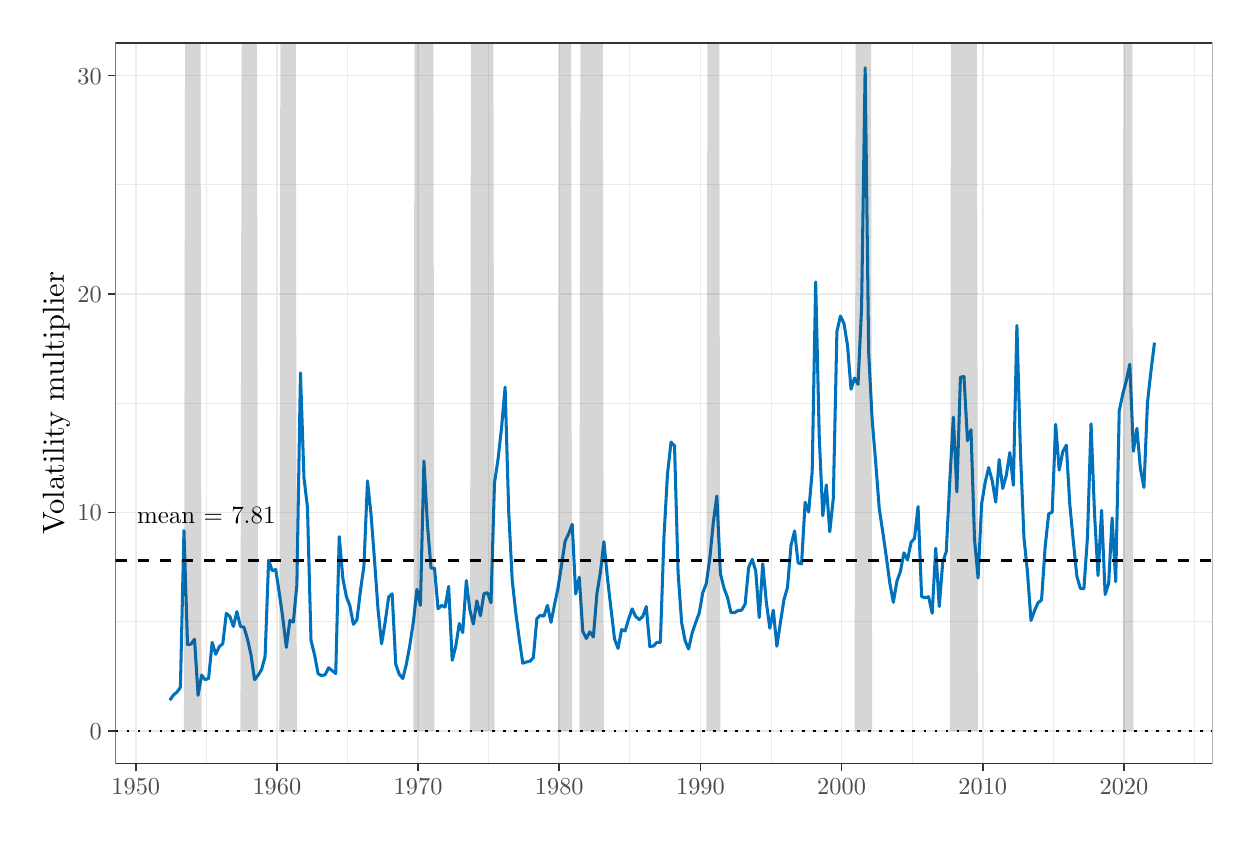
\begin{tikzpicture}[x=1pt,y=1pt]
\definecolor{fillColor}{RGB}{255,255,255}
\path[use as bounding box,fill=fillColor,fill opacity=0.00] (0,0) rectangle (433.62,289.08);
\begin{scope}
\path[clip] (  0.00,  0.00) rectangle (433.62,289.08);
\definecolor{drawColor}{RGB}{255,255,255}
\definecolor{fillColor}{RGB}{255,255,255}

\path[draw=drawColor,line width= 0.6pt,line join=round,line cap=round,fill=fillColor] (  0.00,  0.00) rectangle (433.62,289.08);
\end{scope}
\begin{scope}
\path[clip] ( 31.71, 23.11) rectangle (428.12,283.58);
\definecolor{fillColor}{RGB}{255,255,255}

\path[fill=fillColor] ( 31.71, 23.11) rectangle (428.12,283.58);
\definecolor{drawColor}{gray}{0.92}

\path[draw=drawColor,line width= 0.3pt,line join=round] ( 31.71, 74.41) --
	(428.12, 74.41);

\path[draw=drawColor,line width= 0.3pt,line join=round] ( 31.71,153.34) --
	(428.12,153.34);

\path[draw=drawColor,line width= 0.3pt,line join=round] ( 31.71,232.28) --
	(428.12,232.28);

\path[draw=drawColor,line width= 0.3pt,line join=round] ( 64.56, 23.11) --
	( 64.56,283.58);

\path[draw=drawColor,line width= 0.3pt,line join=round] (115.57, 23.11) --
	(115.57,283.58);

\path[draw=drawColor,line width= 0.3pt,line join=round] (166.59, 23.11) --
	(166.59,283.58);

\path[draw=drawColor,line width= 0.3pt,line join=round] (217.60, 23.11) --
	(217.60,283.58);

\path[draw=drawColor,line width= 0.3pt,line join=round] (268.61, 23.11) --
	(268.61,283.58);

\path[draw=drawColor,line width= 0.3pt,line join=round] (319.62, 23.11) --
	(319.62,283.58);

\path[draw=drawColor,line width= 0.3pt,line join=round] (370.64, 23.11) --
	(370.64,283.58);

\path[draw=drawColor,line width= 0.3pt,line join=round] (421.64, 23.11) --
	(421.64,283.58);

\path[draw=drawColor,line width= 0.6pt,line join=round] ( 31.71, 34.95) --
	(428.12, 34.95);

\path[draw=drawColor,line width= 0.6pt,line join=round] ( 31.71,113.88) --
	(428.12,113.88);

\path[draw=drawColor,line width= 0.6pt,line join=round] ( 31.71,192.81) --
	(428.12,192.81);

\path[draw=drawColor,line width= 0.6pt,line join=round] ( 31.71,271.74) --
	(428.12,271.74);

\path[draw=drawColor,line width= 0.6pt,line join=round] ( 39.06, 23.11) --
	( 39.06,283.58);

\path[draw=drawColor,line width= 0.6pt,line join=round] ( 90.06, 23.11) --
	( 90.06,283.58);

\path[draw=drawColor,line width= 0.6pt,line join=round] (141.08, 23.11) --
	(141.08,283.58);

\path[draw=drawColor,line width= 0.6pt,line join=round] (192.09, 23.11) --
	(192.09,283.58);

\path[draw=drawColor,line width= 0.6pt,line join=round] (243.11, 23.11) --
	(243.11,283.58);

\path[draw=drawColor,line width= 0.6pt,line join=round] (294.11, 23.11) --
	(294.11,283.58);

\path[draw=drawColor,line width= 0.6pt,line join=round] (345.13, 23.11) --
	(345.13,283.58);

\path[draw=drawColor,line width= 0.6pt,line join=round] (396.14, 23.11) --
	(396.14,283.58);
\definecolor{drawColor}{RGB}{0,114,189}

\path[draw=drawColor,line width= 1.1pt,line join=round] ( 51.38, 46.04) --
	( 52.66, 47.92) --
	( 53.93, 48.94) --
	( 55.19, 50.73) --
	( 56.47,107.36) --
	( 57.76, 66.17) --
	( 59.03, 66.34) --
	( 60.29, 68.09) --
	( 61.57, 47.82) --
	( 62.86, 55.13) --
	( 64.13, 53.47) --
	( 65.38, 53.96) --
	( 66.67, 66.96) --
	( 67.95, 62.65) --
	( 69.22, 65.38) --
	( 70.50, 66.45) --
	( 71.78, 77.44) --
	( 73.07, 76.31) --
	( 74.34, 72.68) --
	( 75.59, 78.09) --
	( 76.88, 72.69) --
	( 78.16, 72.45) --
	( 79.43, 68.14) --
	( 80.69, 62.51) --
	( 81.98, 53.49) --
	( 83.26, 55.04) --
	( 84.53, 57.15) --
	( 85.79, 61.88) --
	( 87.07, 96.65) --
	( 88.36, 92.86) --
	( 89.63, 93.25) --
	( 90.90, 84.90) --
	( 92.19, 75.80) --
	( 93.47, 65.15) --
	( 94.74, 74.90) --
	( 96.00, 74.28) --
	( 97.28, 87.82) --
	( 98.57,164.32) --
	( 99.84,126.39) --
	(101.10,115.80) --
	(102.38, 67.66) --
	(103.67, 62.44) --
	(104.94, 55.65) --
	(106.19, 54.93) --
	(107.48, 55.25) --
	(108.76, 57.79) --
	(110.03, 56.74) --
	(111.31, 55.69) --
	(112.59,105.19) --
	(113.88, 90.17) --
	(115.15, 83.51) --
	(116.40, 80.30) --
	(117.69, 73.48) --
	(118.97, 75.10) --
	(120.24, 85.61) --
	(121.50, 94.53) --
	(122.79,125.28) --
	(124.07,113.29) --
	(125.34, 96.52) --
	(126.60, 78.82) --
	(127.88, 66.42) --
	(129.17, 74.21) --
	(130.44, 83.33) --
	(131.71, 84.53) --
	(133.00, 59.04) --
	(134.28, 55.40) --
	(135.55, 53.88) --
	(136.81, 59.00) --
	(138.09, 65.88) --
	(139.38, 74.47) --
	(140.65, 86.13) --
	(141.91, 80.35) --
	(143.19,132.47) --
	(144.48,109.11) --
	(145.75, 93.79) --
	(147.00, 93.81) --
	(148.29, 79.11) --
	(149.57, 80.33) --
	(150.84, 79.69) --
	(152.12, 87.19) --
	(153.40, 60.48) --
	(154.69, 65.54) --
	(155.96, 73.79) --
	(157.21, 70.50) --
	(158.50, 89.30) --
	(159.78, 78.62) --
	(161.05, 73.57) --
	(162.31, 81.95) --
	(163.60, 76.57) --
	(164.88, 84.54) --
	(166.15, 84.92) --
	(167.41, 81.25) --
	(168.69,124.67) --
	(169.98,133.24) --
	(171.25,144.72) --
	(172.52,159.20) --
	(173.81,114.41) --
	(175.09, 89.36) --
	(176.36, 77.86) --
	(177.62, 68.31) --
	(178.90, 59.44) --
	(180.19, 59.86) --
	(181.46, 60.11) --
	(182.72, 61.41) --
	(184.00, 75.59) --
	(185.29, 76.77) --
	(186.56, 76.43) --
	(187.81, 80.34) --
	(189.10, 74.19) --
	(190.38, 80.62) --
	(191.65, 86.70) --
	(192.93, 95.02) --
	(194.21,103.55) --
	(195.50,106.24) --
	(196.77,109.62) --
	(198.02, 84.44) --
	(199.31, 90.53) --
	(200.59, 70.97) --
	(201.86, 68.37) --
	(203.12, 70.77) --
	(204.41, 68.90) --
	(205.69, 84.51) --
	(206.96, 92.28) --
	(208.22,103.34) --
	(209.50, 90.26) --
	(210.79, 79.02) --
	(212.06, 68.19) --
	(213.33, 64.78) --
	(214.62, 71.59) --
	(215.90, 71.11) --
	(217.17, 75.45) --
	(218.43, 79.06) --
	(219.71, 76.33) --
	(221.00, 75.14) --
	(222.27, 76.35) --
	(223.53, 79.89) --
	(224.81, 65.43) --
	(226.10, 65.65) --
	(227.37, 66.94) --
	(228.62, 66.92) --
	(229.91,104.88) --
	(231.19,127.79) --
	(232.47,139.32) --
	(233.74,137.96) --
	(235.02, 92.13) --
	(236.31, 74.07) --
	(237.58, 67.51) --
	(238.83, 64.58) --
	(240.12, 70.42) --
	(241.40, 74.14) --
	(242.67, 77.61) --
	(243.93, 84.85) --
	(245.22, 88.23) --
	(246.50, 97.43) --
	(247.77,110.46) --
	(249.03,119.86) --
	(250.31, 91.89) --
	(251.60, 86.58) --
	(252.87, 83.20) --
	(254.14, 77.70) --
	(255.43, 77.71) --
	(256.71, 78.46) --
	(257.98, 78.60) --
	(259.24, 80.78) --
	(260.52, 94.01) --
	(261.81, 96.94) --
	(263.08, 92.79) --
	(264.34, 75.94) --
	(265.62, 95.34) --
	(266.91, 81.41) --
	(268.18, 72.06) --
	(269.43, 78.57) --
	(270.72, 65.55) --
	(272.00, 74.10) --
	(273.28, 82.34) --
	(274.55, 86.82) --
	(275.83,102.05) --
	(277.12,107.22) --
	(278.39, 95.68) --
	(279.64, 95.33) --
	(280.93,117.59) --
	(282.21,114.06) --
	(283.48,128.77) --
	(284.74,197.19) --
	(286.03,141.29) --
	(287.31,112.71) --
	(288.58,123.87) --
	(289.84,106.92) --
	(291.12,119.08) --
	(292.41,179.23) --
	(293.68,184.88) --
	(294.95,182.22) --
	(296.24,174.31) --
	(297.52,158.42) --
	(298.79,162.48) --
	(300.05,160.19) --
	(301.33,187.92) --
	(302.62,274.60) --
	(303.89,171.71) --
	(305.15,147.57) --
	(306.43,131.95) --
	(307.72,115.27) --
	(308.99,106.81) --
	(310.24, 98.00) --
	(311.53, 88.40) --
	(312.81, 81.43) --
	(314.09, 89.07) --
	(315.36, 92.56) --
	(316.64, 99.33) --
	(317.93, 96.72) --
	(319.20,103.10) --
	(320.45,104.53) --
	(321.74,116.02) --
	(323.02, 83.51) --
	(324.29, 83.06) --
	(325.55, 83.43) --
	(326.84, 77.46) --
	(328.12,100.99) --
	(329.39, 79.90) --
	(330.65, 95.92) --
	(331.93, 99.75) --
	(333.22,125.71) --
	(334.49,148.38) --
	(335.76,121.34) --
	(337.05,162.78) --
	(338.33,163.01) --
	(339.60,139.83) --
	(340.86,143.81) --
	(342.14,104.14) --
	(343.43, 90.21) --
	(344.70,116.95) --
	(345.96,124.65) --
	(347.24,130.15) --
	(348.53,125.38) --
	(349.80,117.64) --
	(351.05,133.01) --
	(352.34,122.57) --
	(353.62,127.25) --
	(354.90,135.57) --
	(356.17,123.71) --
	(357.45,181.47) --
	(358.74,135.49) --
	(360.01,104.75) --
	(361.26, 92.42) --
	(362.55, 74.86) --
	(363.83, 78.44) --
	(365.10, 81.29) --
	(366.36, 82.26) --
	(367.65,101.35) --
	(368.93,113.41) --
	(370.20,113.98) --
	(371.46,145.74) --
	(372.74,129.18) --
	(374.03,135.87) --
	(375.30,138.21) --
	(376.57,116.84) --
	(377.86,103.29) --
	(379.14, 90.72) --
	(380.41, 86.41) --
	(381.67, 86.35) --
	(382.95,104.94) --
	(384.24,145.94) --
	(385.51,113.26) --
	(386.77, 91.11) --
	(388.05,114.68) --
	(389.34, 84.25) --
	(390.61, 88.31) --
	(391.86,111.92) --
	(393.15, 88.88) --
	(394.43,150.61) --
	(395.71,156.70) --
	(396.98,161.47) --
	(398.26,167.46) --
	(399.55,136.03) --
	(400.82,144.31) --
	(402.07,129.83) --
	(403.36,122.94) --
	(404.64,153.67) --
	(405.91,165.12) --
	(407.17,175.26);
\definecolor{fillColor}{RGB}{51,51,51}

\path[fill=fillColor,fill opacity=0.20] ( 50.09, 34.95) --
	( 50.45, 34.95) --
	( 51.02, 34.95) --
	( 51.38, 34.95) --
	( 51.73, 34.95) --
	( 52.30, 34.95) --
	( 52.66, 34.95) --
	( 53.02, 34.95) --
	( 53.57, 34.95) --
	( 53.93, 34.95) --
	( 54.29, 34.95) --
	( 54.83, 34.95) --
	( 55.19, 34.95) --
	( 55.55, 34.95) --
	( 56.11, 34.95) --
	( 56.47, 34.95) --
	( 56.83,255.88) --
	( 57.40,603.33) --
	( 57.76,824.25) --
	( 58.12,824.25) --
	( 58.67,824.25) --
	( 59.03,824.25) --
	( 59.39,824.25) --
	( 59.93,824.25) --
	( 60.29,824.25) --
	( 60.65,824.25) --
	( 61.21,824.25) --
	( 61.57,824.25) --
	( 61.93,603.33) --
	( 62.50,255.88) --
	( 62.86, 34.95) --
	( 63.22, 34.95) --
	( 63.77, 34.95) --
	( 64.13, 34.95) --
	( 64.49, 34.95) --
	( 65.02, 34.95) --
	( 65.38, 34.95) --
	( 65.74, 34.95) --
	( 66.31, 34.95) --
	( 66.67, 34.95) --
	( 67.03, 34.95) --
	( 67.59, 34.95) --
	( 67.95, 34.95) --
	( 68.31, 34.95) --
	( 68.86, 34.95) --
	( 69.22, 34.95) --
	( 69.58, 34.95) --
	( 70.14, 34.95) --
	( 70.50, 34.95) --
	( 70.86, 34.95) --
	( 71.42, 34.95) --
	( 71.78, 34.95) --
	( 72.14, 34.95) --
	( 72.71, 34.95) --
	( 73.07, 34.95) --
	( 73.42, 34.95) --
	( 73.98, 34.95) --
	( 74.34, 34.95) --
	( 74.70, 34.95) --
	( 75.23, 34.95) --
	( 75.59, 34.95) --
	( 75.95, 34.95) --
	( 76.52, 34.95) --
	( 76.88, 34.95) --
	( 77.24,255.88) --
	( 77.80,603.33) --
	( 78.16,824.25) --
	( 78.52,824.25) --
	( 79.07,824.25) --
	( 79.43,824.25) --
	( 79.79,824.25) --
	( 80.33,824.25) --
	( 80.69,824.25) --
	( 81.05,824.25) --
	( 81.62,824.25) --
	( 81.98,824.25) --
	( 82.34,603.33) --
	( 82.90,255.88) --
	( 83.26, 34.95) --
	( 83.62, 34.95) --
	( 84.17, 34.95) --
	( 84.53, 34.95) --
	( 84.89, 34.95) --
	( 85.43, 34.95) --
	( 85.79, 34.95) --
	( 86.15, 34.95) --
	( 86.71, 34.95) --
	( 87.07, 34.95) --
	( 87.43, 34.95) --
	( 88.00, 34.95) --
	( 88.36, 34.95) --
	( 88.72, 34.95) --
	( 89.27, 34.95) --
	( 89.63, 34.95) --
	( 89.99, 34.95) --
	( 90.54, 34.95) --
	( 90.90, 34.95) --
	( 91.26,255.88) --
	( 91.83,603.33) --
	( 92.19,824.25) --
	( 92.55,824.25) --
	( 93.11,824.25) --
	( 93.47,824.25) --
	( 93.83,824.25) --
	( 94.38,824.25) --
	( 94.74,824.25) --
	( 95.10,824.25) --
	( 95.64,824.25) --
	( 96.00,824.25) --
	( 96.36,603.33) --
	( 96.92,255.88) --
	( 97.28, 34.95) --
	( 97.64, 34.95) --
	( 98.21, 34.95) --
	( 98.57, 34.95) --
	( 98.93, 34.95) --
	( 99.48, 34.95) --
	( 99.84, 34.95) --
	(100.20, 34.95) --
	(100.74, 34.95) --
	(101.10, 34.95) --
	(101.46, 34.95) --
	(102.02, 34.95) --
	(102.38, 34.95) --
	(102.74, 34.95) --
	(103.31, 34.95) --
	(103.67, 34.95) --
	(104.03, 34.95) --
	(104.58, 34.95) --
	(104.94, 34.95) --
	(105.30, 34.95) --
	(105.83, 34.95) --
	(106.19, 34.95) --
	(106.55, 34.95) --
	(107.12, 34.95) --
	(107.48, 34.95) --
	(107.84, 34.95) --
	(108.40, 34.95) --
	(108.76, 34.95) --
	(109.12, 34.95) --
	(109.67, 34.95) --
	(110.03, 34.95) --
	(110.39, 34.95) --
	(110.95, 34.95) --
	(111.31, 34.95) --
	(111.67, 34.95) --
	(112.23, 34.95) --
	(112.59, 34.95) --
	(112.95, 34.95) --
	(113.52, 34.95) --
	(113.88, 34.95) --
	(114.24, 34.95) --
	(114.79, 34.95) --
	(115.15, 34.95) --
	(115.51, 34.95) --
	(116.04, 34.95) --
	(116.40, 34.95) --
	(116.76, 34.95) --
	(117.33, 34.95) --
	(117.69, 34.95) --
	(118.05, 34.95) --
	(118.61, 34.95) --
	(118.97, 34.95) --
	(119.33, 34.95) --
	(119.88, 34.95) --
	(120.24, 34.95) --
	(120.60, 34.95) --
	(121.14, 34.95) --
	(121.50, 34.95) --
	(121.86, 34.95) --
	(122.43, 34.95) --
	(122.79, 34.95) --
	(123.15, 34.95) --
	(123.71, 34.95) --
	(124.07, 34.95) --
	(124.43, 34.95) --
	(124.98, 34.95) --
	(125.34, 34.95) --
	(125.70, 34.95) --
	(126.24, 34.95) --
	(126.60, 34.95) --
	(126.96, 34.95) --
	(127.52, 34.95) --
	(127.88, 34.95) --
	(128.24, 34.95) --
	(128.81, 34.95) --
	(129.17, 34.95) --
	(129.53, 34.95) --
	(130.08, 34.95) --
	(130.44, 34.95) --
	(130.80, 34.95) --
	(131.35, 34.95) --
	(131.71, 34.95) --
	(132.07, 34.95) --
	(132.64, 34.95) --
	(133.00, 34.95) --
	(133.36, 34.95) --
	(133.92, 34.95) --
	(134.28, 34.95) --
	(134.64, 34.95) --
	(135.19, 34.95) --
	(135.55, 34.95) --
	(135.91, 34.95) --
	(136.45, 34.95) --
	(136.81, 34.95) --
	(137.17, 34.95) --
	(137.73, 34.95) --
	(138.09, 34.95) --
	(138.45, 34.95) --
	(139.02, 34.95) --
	(139.38, 34.95) --
	(139.74,258.30) --
	(140.29,600.90) --
	(140.65,824.25) --
	(141.01,824.25) --
	(141.55,824.25) --
	(141.91,824.25) --
	(142.27,824.25) --
	(142.83,824.25) --
	(143.19,824.25) --
	(143.55,824.25) --
	(144.12,824.25) --
	(144.48,824.25) --
	(144.84,824.25) --
	(145.39,824.25) --
	(145.75,824.25) --
	(146.11,598.42) --
	(146.64,260.79) --
	(147.00, 34.95) --
	(147.36, 34.95) --
	(147.93, 34.95) --
	(148.29, 34.95) --
	(148.65, 34.95) --
	(149.21, 34.95) --
	(149.57, 34.95) --
	(149.93, 34.95) --
	(150.49, 34.95) --
	(150.84, 34.95) --
	(151.20, 34.95) --
	(151.76, 34.95) --
	(152.12, 34.95) --
	(152.48, 34.95) --
	(153.04, 34.95) --
	(153.40, 34.95) --
	(153.76, 34.95) --
	(154.33, 34.95) --
	(154.69, 34.95) --
	(155.05, 34.95) --
	(155.60, 34.95) --
	(155.96, 34.95) --
	(156.32, 34.95) --
	(156.85, 34.95) --
	(157.21, 34.95) --
	(157.57, 34.95) --
	(158.14, 34.95) --
	(158.50, 34.95) --
	(158.86, 34.95) --
	(159.42, 34.95) --
	(159.78, 34.95) --
	(160.14,258.30) --
	(160.69,600.90) --
	(161.05,824.25) --
	(161.41,824.25) --
	(161.95,824.25) --
	(162.31,824.25) --
	(162.67,824.25) --
	(163.24,824.25) --
	(163.60,824.25) --
	(163.96,824.25) --
	(164.52,824.25) --
	(164.88,824.25) --
	(165.24,824.25) --
	(165.79,824.25) --
	(166.15,824.25) --
	(166.51,824.25) --
	(167.05,824.25) --
	(167.41,824.25) --
	(167.77,603.33) --
	(168.33,255.88) --
	(168.69, 34.95) --
	(169.05, 34.95) --
	(169.62, 34.95) --
	(169.98, 34.95) --
	(170.34, 34.95) --
	(170.89, 34.95) --
	(171.25, 34.95) --
	(171.61, 34.95) --
	(172.16, 34.95) --
	(172.52, 34.95) --
	(172.88, 34.95) --
	(173.45, 34.95) --
	(173.81, 34.95) --
	(174.17, 34.95) --
	(174.73, 34.95) --
	(175.09, 34.95) --
	(175.45, 34.95) --
	(176.00, 34.95) --
	(176.36, 34.95) --
	(176.72, 34.95) --
	(177.26, 34.95) --
	(177.62, 34.95) --
	(177.98, 34.95) --
	(178.54, 34.95) --
	(178.90, 34.95) --
	(179.26, 34.95) --
	(179.83, 34.95) --
	(180.19, 34.95) --
	(180.55, 34.95) --
	(181.10, 34.95) --
	(181.46, 34.95) --
	(181.82, 34.95) --
	(182.36, 34.95) --
	(182.72, 34.95) --
	(183.08, 34.95) --
	(183.64, 34.95) --
	(184.00, 34.95) --
	(184.36, 34.95) --
	(184.93, 34.95) --
	(185.29, 34.95) --
	(185.65, 34.95) --
	(186.20, 34.95) --
	(186.56, 34.95) --
	(186.92, 34.95) --
	(187.45, 34.95) --
	(187.81, 34.95) --
	(188.17, 34.95) --
	(188.74, 34.95) --
	(189.10, 34.95) --
	(189.46, 34.95) --
	(190.02, 34.95) --
	(190.38, 34.95) --
	(190.74, 34.95) --
	(191.30, 34.95) --
	(191.65, 34.95) --
	(192.01,258.30) --
	(192.57,600.90) --
	(192.93,824.25) --
	(193.29,824.25) --
	(193.85,824.25) --
	(194.21,824.25) --
	(194.57,824.25) --
	(195.14,824.25) --
	(195.50,824.25) --
	(195.86,600.90) --
	(196.41,258.30) --
	(196.77, 34.95) --
	(197.13, 34.95) --
	(197.66, 34.95) --
	(198.02, 34.95) --
	(198.38, 34.95) --
	(198.95, 34.95) --
	(199.31, 34.95) --
	(199.67,255.88) --
	(200.23,603.33) --
	(200.59,824.25) --
	(200.95,824.25) --
	(201.50,824.25) --
	(201.86,824.25) --
	(202.22,824.25) --
	(202.76,824.25) --
	(203.12,824.25) --
	(203.48,824.25) --
	(204.05,824.25) --
	(204.41,824.25) --
	(204.77,824.25) --
	(205.33,824.25) --
	(205.69,824.25) --
	(206.05,824.25) --
	(206.60,824.25) --
	(206.96,824.25) --
	(207.32,598.42) --
	(207.86,260.79) --
	(208.22, 34.95) --
	(208.58, 34.95) --
	(209.14, 34.95) --
	(209.50, 34.95) --
	(209.86, 34.95) --
	(210.43, 34.95) --
	(210.79, 34.95) --
	(211.15, 34.95) --
	(211.70, 34.95) --
	(212.06, 34.95) --
	(212.42, 34.95) --
	(212.97, 34.95) --
	(213.33, 34.95) --
	(213.69, 34.95) --
	(214.26, 34.95) --
	(214.62, 34.95) --
	(214.98, 34.95) --
	(215.54, 34.95) --
	(215.90, 34.95) --
	(216.26, 34.95) --
	(216.81, 34.95) --
	(217.17, 34.95) --
	(217.53, 34.95) --
	(218.07, 34.95) --
	(218.43, 34.95) --
	(218.79, 34.95) --
	(219.35, 34.95) --
	(219.71, 34.95) --
	(220.07, 34.95) --
	(220.64, 34.95) --
	(221.00, 34.95) --
	(221.36, 34.95) --
	(221.91, 34.95) --
	(222.27, 34.95) --
	(222.63, 34.95) --
	(223.17, 34.95) --
	(223.53, 34.95) --
	(223.89, 34.95) --
	(224.45, 34.95) --
	(224.81, 34.95) --
	(225.17, 34.95) --
	(225.74, 34.95) --
	(226.10, 34.95) --
	(226.46, 34.95) --
	(227.01, 34.95) --
	(227.37, 34.95) --
	(227.73, 34.95) --
	(228.26, 34.95) --
	(228.62, 34.95) --
	(228.98, 34.95) --
	(229.55, 34.95) --
	(229.91, 34.95) --
	(230.27, 34.95) --
	(230.83, 34.95) --
	(231.19, 34.95) --
	(231.55, 34.95) --
	(232.11, 34.95) --
	(232.47, 34.95) --
	(232.82, 34.95) --
	(233.38, 34.95) --
	(233.74, 34.95) --
	(234.10, 34.95) --
	(234.66, 34.95) --
	(235.02, 34.95) --
	(235.38, 34.95) --
	(235.95, 34.95) --
	(236.31, 34.95) --
	(236.67, 34.95) --
	(237.22, 34.95) --
	(237.58, 34.95) --
	(237.94, 34.95) --
	(238.47, 34.95) --
	(238.83, 34.95) --
	(239.19, 34.95) --
	(239.76, 34.95) --
	(240.12, 34.95) --
	(240.48, 34.95) --
	(241.04, 34.95) --
	(241.40, 34.95) --
	(241.76, 34.95) --
	(242.31, 34.95) --
	(242.67, 34.95) --
	(243.03, 34.95) --
	(243.57, 34.95) --
	(243.93, 34.95) --
	(244.29, 34.95) --
	(244.86, 34.95) --
	(245.22, 34.95) --
	(245.58,255.88) --
	(246.14,603.33) --
	(246.50,824.25) --
	(246.86,824.25) --
	(247.41,824.25) --
	(247.77,824.25) --
	(248.13,824.25) --
	(248.67,824.25) --
	(249.03,824.25) --
	(249.39,603.33) --
	(249.95,255.88) --
	(250.31, 34.95) --
	(250.67, 34.95) --
	(251.24, 34.95) --
	(251.60, 34.95) --
	(251.96, 34.95) --
	(252.51, 34.95) --
	(252.87, 34.95) --
	(253.23, 34.95) --
	(253.78, 34.95) --
	(254.14, 34.95) --
	(254.50, 34.95) --
	(255.07, 34.95) --
	(255.43, 34.95) --
	(255.79, 34.95) --
	(256.35, 34.95) --
	(256.71, 34.95) --
	(257.07, 34.95) --
	(257.62, 34.95) --
	(257.98, 34.95) --
	(258.34, 34.95) --
	(258.88, 34.95) --
	(259.24, 34.95) --
	(259.60, 34.95) --
	(260.16, 34.95) --
	(260.52, 34.95) --
	(260.88, 34.95) --
	(261.45, 34.95) --
	(261.81, 34.95) --
	(262.17, 34.95) --
	(262.72, 34.95) --
	(263.08, 34.95) --
	(263.44, 34.95) --
	(263.98, 34.95) --
	(264.34, 34.95) --
	(264.70, 34.95) --
	(265.26, 34.95) --
	(265.62, 34.95) --
	(265.98, 34.95) --
	(266.55, 34.95) --
	(266.91, 34.95) --
	(267.27, 34.95) --
	(267.82, 34.95) --
	(268.18, 34.95) --
	(268.54, 34.95) --
	(269.07, 34.95) --
	(269.43, 34.95) --
	(269.79, 34.95) --
	(270.36, 34.95) --
	(270.72, 34.95) --
	(271.08, 34.95) --
	(271.64, 34.95) --
	(272.00, 34.95) --
	(272.36, 34.95) --
	(272.92, 34.95) --
	(273.28, 34.95) --
	(273.63, 34.95) --
	(274.19, 34.95) --
	(274.55, 34.95) --
	(274.91, 34.95) --
	(275.47, 34.95) --
	(275.83, 34.95) --
	(276.19, 34.95) --
	(276.76, 34.95) --
	(277.12, 34.95) --
	(277.48, 34.95) --
	(278.03, 34.95) --
	(278.39, 34.95) --
	(278.75, 34.95) --
	(279.28, 34.95) --
	(279.64, 34.95) --
	(280.00, 34.95) --
	(280.57, 34.95) --
	(280.93, 34.95) --
	(281.29, 34.95) --
	(281.85, 34.95) --
	(282.21, 34.95) --
	(282.57, 34.95) --
	(283.12, 34.95) --
	(283.48, 34.95) --
	(283.84, 34.95) --
	(284.38, 34.95) --
	(284.74, 34.95) --
	(285.10, 34.95) --
	(285.67, 34.95) --
	(286.03, 34.95) --
	(286.39, 34.95) --
	(286.95, 34.95) --
	(287.31, 34.95) --
	(287.67, 34.95) --
	(288.22, 34.95) --
	(288.58, 34.95) --
	(288.94, 34.95) --
	(289.48, 34.95) --
	(289.84, 34.95) --
	(290.20, 34.95) --
	(290.76, 34.95) --
	(291.12, 34.95) --
	(291.48, 34.95) --
	(292.05, 34.95) --
	(292.41, 34.95) --
	(292.77, 34.95) --
	(293.32, 34.95) --
	(293.68, 34.95) --
	(294.04, 34.95) --
	(294.59, 34.95) --
	(294.95, 34.95) --
	(295.31, 34.95) --
	(295.88, 34.95) --
	(296.24, 34.95) --
	(296.60, 34.95) --
	(297.16, 34.95) --
	(297.52, 34.95) --
	(297.88, 34.95) --
	(298.43, 34.95) --
	(298.79, 34.95) --
	(299.15,260.79) --
	(299.69,598.42) --
	(300.05,824.25) --
	(300.41,824.25) --
	(300.97,824.25) --
	(301.33,824.25) --
	(301.69,824.25) --
	(302.26,824.25) --
	(302.62,824.25) --
	(302.98,824.25) --
	(303.53,824.25) --
	(303.89,824.25) --
	(304.25,598.42) --
	(304.79,260.79) --
	(305.15, 34.95) --
	(305.51, 34.95) --
	(306.07, 34.95) --
	(306.43, 34.95) --
	(306.79, 34.95) --
	(307.36, 34.95) --
	(307.72, 34.95) --
	(308.08, 34.95) --
	(308.63, 34.95) --
	(308.99, 34.95) --
	(309.35, 34.95) --
	(309.88, 34.95) --
	(310.24, 34.95) --
	(310.60, 34.95) --
	(311.17, 34.95) --
	(311.53, 34.95) --
	(311.89, 34.95) --
	(312.45, 34.95) --
	(312.81, 34.95) --
	(313.17, 34.95) --
	(313.73, 34.95) --
	(314.09, 34.95) --
	(314.44, 34.95) --
	(315.00, 34.95) --
	(315.36, 34.95) --
	(315.72, 34.95) --
	(316.28, 34.95) --
	(316.64, 34.95) --
	(317.00, 34.95) --
	(317.57, 34.95) --
	(317.93, 34.95) --
	(318.29, 34.95) --
	(318.84, 34.95) --
	(319.20, 34.95) --
	(319.56, 34.95) --
	(320.09, 34.95) --
	(320.45, 34.95) --
	(320.81, 34.95) --
	(321.38, 34.95) --
	(321.74, 34.95) --
	(322.10, 34.95) --
	(322.66, 34.95) --
	(323.02, 34.95) --
	(323.38, 34.95) --
	(323.94, 34.95) --
	(324.29, 34.95) --
	(324.65, 34.95) --
	(325.19, 34.95) --
	(325.55, 34.95) --
	(325.91, 34.95) --
	(326.48, 34.95) --
	(326.84, 34.95) --
	(327.20, 34.95) --
	(327.76, 34.95) --
	(328.12, 34.95) --
	(328.48, 34.95) --
	(329.03, 34.95) --
	(329.39, 34.95) --
	(329.75, 34.95) --
	(330.29, 34.95) --
	(330.65, 34.95) --
	(331.01, 34.95) --
	(331.57, 34.95) --
	(331.93, 34.95) --
	(332.29, 34.95) --
	(332.86, 34.95) --
	(333.22, 34.95) --
	(333.58,258.30) --
	(334.13,600.90) --
	(334.49,824.25) --
	(334.85,824.25) --
	(335.40,824.25) --
	(335.76,824.25) --
	(336.12,824.25) --
	(336.69,824.25) --
	(337.05,824.25) --
	(337.41,824.25) --
	(337.97,824.25) --
	(338.33,824.25) --
	(338.69,824.25) --
	(339.24,824.25) --
	(339.60,824.25) --
	(339.96,824.25) --
	(340.50,824.25) --
	(340.86,824.25) --
	(341.22,824.25) --
	(341.78,824.25) --
	(342.14,824.25) --
	(342.50,603.33) --
	(343.07,255.88) --
	(343.43, 34.95) --
	(343.79, 34.95) --
	(344.34, 34.95) --
	(344.70, 34.95) --
	(345.06, 34.95) --
	(345.60, 34.95) --
	(345.96, 34.95) --
	(346.32, 34.95) --
	(346.88, 34.95) --
	(347.24, 34.95) --
	(347.60, 34.95) --
	(348.17, 34.95) --
	(348.53, 34.95) --
	(348.89, 34.95) --
	(349.44, 34.95) --
	(349.80, 34.95) --
	(350.16, 34.95) --
	(350.69, 34.95) --
	(351.05, 34.95) --
	(351.41, 34.95) --
	(351.98, 34.95) --
	(352.34, 34.95) --
	(352.70, 34.95) --
	(353.26, 34.95) --
	(353.62, 34.95) --
	(353.98, 34.95) --
	(354.54, 34.95) --
	(354.90, 34.95) --
	(355.26, 34.95) --
	(355.81, 34.95) --
	(356.17, 34.95) --
	(356.53, 34.95) --
	(357.09, 34.95) --
	(357.45, 34.95) --
	(357.81, 34.95) --
	(358.38, 34.95) --
	(358.74, 34.95) --
	(359.10, 34.95) --
	(359.65, 34.95) --
	(360.01, 34.95) --
	(360.37, 34.95) --
	(360.90, 34.95) --
	(361.26, 34.95) --
	(361.62, 34.95) --
	(362.19, 34.95) --
	(362.55, 34.95) --
	(362.91, 34.95) --
	(363.47, 34.95) --
	(363.83, 34.95) --
	(364.19, 34.95) --
	(364.75, 34.95) --
	(365.10, 34.95) --
	(365.46, 34.95) --
	(366.00, 34.95) --
	(366.36, 34.95) --
	(366.72, 34.95) --
	(367.29, 34.95) --
	(367.65, 34.95) --
	(368.01, 34.95) --
	(368.57, 34.95) --
	(368.93, 34.95) --
	(369.29, 34.95) --
	(369.84, 34.95) --
	(370.20, 34.95) --
	(370.56, 34.95) --
	(371.10, 34.95) --
	(371.46, 34.95) --
	(371.82, 34.95) --
	(372.38, 34.95) --
	(372.74, 34.95) --
	(373.10, 34.95) --
	(373.67, 34.95) --
	(374.03, 34.95) --
	(374.39, 34.95) --
	(374.94, 34.95) --
	(375.30, 34.95) --
	(375.66, 34.95) --
	(376.21, 34.95) --
	(376.57, 34.95) --
	(376.93, 34.95) --
	(377.50, 34.95) --
	(377.86, 34.95) --
	(378.22, 34.95) --
	(378.78, 34.95) --
	(379.14, 34.95) --
	(379.50, 34.95) --
	(380.05, 34.95) --
	(380.41, 34.95) --
	(380.77, 34.95) --
	(381.31, 34.95) --
	(381.67, 34.95) --
	(382.03, 34.95) --
	(382.59, 34.95) --
	(382.95, 34.95) --
	(383.31, 34.95) --
	(383.88, 34.95) --
	(384.24, 34.95) --
	(384.60, 34.95) --
	(385.15, 34.95) --
	(385.51, 34.95) --
	(385.87, 34.95) --
	(386.41, 34.95) --
	(386.77, 34.95) --
	(387.13, 34.95) --
	(387.69, 34.95) --
	(388.05, 34.95) --
	(388.41, 34.95) --
	(388.98, 34.95) --
	(389.34, 34.95) --
	(389.70, 34.95) --
	(390.25, 34.95) --
	(390.61, 34.95) --
	(390.97, 34.95) --
	(391.51, 34.95) --
	(391.86, 34.95) --
	(392.22, 34.95) --
	(392.79, 34.95) --
	(393.15, 34.95) --
	(393.51, 34.95) --
	(394.07, 34.95) --
	(394.43, 34.95) --
	(394.79, 34.95) --
	(395.35, 34.95) --
	(395.71, 34.95) --
	(396.07,258.30) --
	(396.62,600.90) --
	(396.98,824.25) --
	(397.34,824.25) --
	(397.90,824.25) --
	(398.26,824.25) --
	(398.62,603.33) --
	(399.19,255.88) --
	(399.55, 34.95) --
	(399.91, 34.95) --
	(400.46, 34.95) --
	(400.82, 34.95) --
	(401.18, 34.95) --
	(401.71, 34.95) --
	(402.07, 34.95) --
	(402.43, 34.95) --
	(403.00, 34.95) --
	(403.36, 34.95) --
	(403.72, 34.95) --
	(404.28, 34.95) --
	(404.64, 34.95) --
	(405.00, 34.95) --
	(405.56, 34.95) --
	(405.91, 34.95) --
	(406.27, 34.95) --
	(406.81, 34.95) --
	(407.17, 34.95) --
	(407.53, 34.95) --
	(408.10, 34.95) --
	(408.46, 34.95) --
	(408.82, 34.95) --
	(409.38, 34.95) --
	(409.74, 34.95) --
	(410.10, 34.95) --
	(409.74, 34.95) --
	(409.38, 34.95) --
	(408.82, 34.95) --
	(408.46, 34.95) --
	(408.10, 34.95) --
	(407.53, 34.95) --
	(407.17, 34.95) --
	(406.81, 34.95) --
	(406.27, 34.95) --
	(405.91, 34.95) --
	(405.56, 34.95) --
	(405.00, 34.95) --
	(404.64, 34.95) --
	(404.28, 34.95) --
	(403.72, 34.95) --
	(403.36, 34.95) --
	(403.00, 34.95) --
	(402.43, 34.95) --
	(402.07, 34.95) --
	(401.71, 34.95) --
	(401.18, 34.95) --
	(400.82, 34.95) --
	(400.46, 34.95) --
	(399.91, 34.95) --
	(399.55, 34.95) --
	(399.19, 34.95) --
	(398.62, 34.95) --
	(398.26, 34.95) --
	(397.90, 34.95) --
	(397.34, 34.95) --
	(396.98, 34.95) --
	(396.62, 34.95) --
	(396.07, 34.95) --
	(395.71, 34.95) --
	(395.35, 34.95) --
	(394.79, 34.95) --
	(394.43, 34.95) --
	(394.07, 34.95) --
	(393.51, 34.95) --
	(393.15, 34.95) --
	(392.79, 34.95) --
	(392.22, 34.95) --
	(391.86, 34.95) --
	(391.51, 34.95) --
	(390.97, 34.95) --
	(390.61, 34.95) --
	(390.25, 34.95) --
	(389.70, 34.95) --
	(389.34, 34.95) --
	(388.98, 34.95) --
	(388.41, 34.95) --
	(388.05, 34.95) --
	(387.69, 34.95) --
	(387.13, 34.95) --
	(386.77, 34.95) --
	(386.41, 34.95) --
	(385.87, 34.95) --
	(385.51, 34.95) --
	(385.15, 34.95) --
	(384.60, 34.95) --
	(384.24, 34.95) --
	(383.88, 34.95) --
	(383.31, 34.95) --
	(382.95, 34.95) --
	(382.59, 34.95) --
	(382.03, 34.95) --
	(381.67, 34.95) --
	(381.31, 34.95) --
	(380.77, 34.95) --
	(380.41, 34.95) --
	(380.05, 34.95) --
	(379.50, 34.95) --
	(379.14, 34.95) --
	(378.78, 34.95) --
	(378.22, 34.95) --
	(377.86, 34.95) --
	(377.50, 34.95) --
	(376.93, 34.95) --
	(376.57, 34.95) --
	(376.21, 34.95) --
	(375.66, 34.95) --
	(375.30, 34.95) --
	(374.94, 34.95) --
	(374.39, 34.95) --
	(374.03, 34.95) --
	(373.67, 34.95) --
	(373.10, 34.95) --
	(372.74, 34.95) --
	(372.38, 34.95) --
	(371.82, 34.95) --
	(371.46, 34.95) --
	(371.10, 34.95) --
	(370.56, 34.95) --
	(370.20, 34.95) --
	(369.84, 34.95) --
	(369.29, 34.95) --
	(368.93, 34.95) --
	(368.57, 34.95) --
	(368.01, 34.95) --
	(367.65, 34.95) --
	(367.29, 34.95) --
	(366.72, 34.95) --
	(366.36, 34.95) --
	(366.00, 34.95) --
	(365.46, 34.95) --
	(365.10, 34.95) --
	(364.75, 34.95) --
	(364.19, 34.95) --
	(363.83, 34.95) --
	(363.47, 34.95) --
	(362.91, 34.95) --
	(362.55, 34.95) --
	(362.19, 34.95) --
	(361.62, 34.95) --
	(361.26, 34.95) --
	(360.90, 34.95) --
	(360.37, 34.95) --
	(360.01, 34.95) --
	(359.65, 34.95) --
	(359.10, 34.95) --
	(358.74, 34.95) --
	(358.38, 34.95) --
	(357.81, 34.95) --
	(357.45, 34.95) --
	(357.09, 34.95) --
	(356.53, 34.95) --
	(356.17, 34.95) --
	(355.81, 34.95) --
	(355.26, 34.95) --
	(354.90, 34.95) --
	(354.54, 34.95) --
	(353.98, 34.95) --
	(353.62, 34.95) --
	(353.26, 34.95) --
	(352.70, 34.95) --
	(352.34, 34.95) --
	(351.98, 34.95) --
	(351.41, 34.95) --
	(351.05, 34.95) --
	(350.69, 34.95) --
	(350.16, 34.95) --
	(349.80, 34.95) --
	(349.44, 34.95) --
	(348.89, 34.95) --
	(348.53, 34.95) --
	(348.17, 34.95) --
	(347.60, 34.95) --
	(347.24, 34.95) --
	(346.88, 34.95) --
	(346.32, 34.95) --
	(345.96, 34.95) --
	(345.60, 34.95) --
	(345.06, 34.95) --
	(344.70, 34.95) --
	(344.34, 34.95) --
	(343.79, 34.95) --
	(343.43, 34.95) --
	(343.07, 34.95) --
	(342.50, 34.95) --
	(342.14, 34.95) --
	(341.78, 34.95) --
	(341.22, 34.95) --
	(340.86, 34.95) --
	(340.50, 34.95) --
	(339.96, 34.95) --
	(339.60, 34.95) --
	(339.24, 34.95) --
	(338.69, 34.95) --
	(338.33, 34.95) --
	(337.97, 34.95) --
	(337.41, 34.95) --
	(337.05, 34.95) --
	(336.69, 34.95) --
	(336.12, 34.95) --
	(335.76, 34.95) --
	(335.40, 34.95) --
	(334.85, 34.95) --
	(334.49, 34.95) --
	(334.13, 34.95) --
	(333.58, 34.95) --
	(333.22, 34.95) --
	(332.86, 34.95) --
	(332.29, 34.95) --
	(331.93, 34.95) --
	(331.57, 34.95) --
	(331.01, 34.95) --
	(330.65, 34.95) --
	(330.29, 34.95) --
	(329.75, 34.95) --
	(329.39, 34.95) --
	(329.03, 34.95) --
	(328.48, 34.95) --
	(328.12, 34.95) --
	(327.76, 34.95) --
	(327.20, 34.95) --
	(326.84, 34.95) --
	(326.48, 34.95) --
	(325.91, 34.95) --
	(325.55, 34.95) --
	(325.19, 34.95) --
	(324.65, 34.95) --
	(324.29, 34.95) --
	(323.94, 34.95) --
	(323.38, 34.95) --
	(323.02, 34.95) --
	(322.66, 34.95) --
	(322.10, 34.95) --
	(321.74, 34.95) --
	(321.38, 34.95) --
	(320.81, 34.95) --
	(320.45, 34.95) --
	(320.09, 34.95) --
	(319.56, 34.95) --
	(319.20, 34.95) --
	(318.84, 34.95) --
	(318.29, 34.95) --
	(317.93, 34.95) --
	(317.57, 34.95) --
	(317.00, 34.95) --
	(316.64, 34.95) --
	(316.28, 34.95) --
	(315.72, 34.95) --
	(315.36, 34.95) --
	(315.00, 34.95) --
	(314.44, 34.95) --
	(314.09, 34.95) --
	(313.73, 34.95) --
	(313.17, 34.95) --
	(312.81, 34.95) --
	(312.45, 34.95) --
	(311.89, 34.95) --
	(311.53, 34.95) --
	(311.17, 34.95) --
	(310.60, 34.95) --
	(310.24, 34.95) --
	(309.88, 34.95) --
	(309.35, 34.95) --
	(308.99, 34.95) --
	(308.63, 34.95) --
	(308.08, 34.95) --
	(307.72, 34.95) --
	(307.36, 34.95) --
	(306.79, 34.95) --
	(306.43, 34.95) --
	(306.07, 34.95) --
	(305.51, 34.95) --
	(305.15, 34.95) --
	(304.79, 34.95) --
	(304.25, 34.95) --
	(303.89, 34.95) --
	(303.53, 34.95) --
	(302.98, 34.95) --
	(302.62, 34.95) --
	(302.26, 34.95) --
	(301.69, 34.95) --
	(301.33, 34.95) --
	(300.97, 34.95) --
	(300.41, 34.95) --
	(300.05, 34.95) --
	(299.69, 34.95) --
	(299.15, 34.95) --
	(298.79, 34.95) --
	(298.43, 34.95) --
	(297.88, 34.95) --
	(297.52, 34.95) --
	(297.16, 34.95) --
	(296.60, 34.95) --
	(296.24, 34.95) --
	(295.88, 34.95) --
	(295.31, 34.95) --
	(294.95, 34.95) --
	(294.59, 34.95) --
	(294.04, 34.95) --
	(293.68, 34.95) --
	(293.32, 34.95) --
	(292.77, 34.95) --
	(292.41, 34.95) --
	(292.05, 34.95) --
	(291.48, 34.95) --
	(291.12, 34.95) --
	(290.76, 34.95) --
	(290.20, 34.95) --
	(289.84, 34.95) --
	(289.48, 34.95) --
	(288.94, 34.95) --
	(288.58, 34.95) --
	(288.22, 34.95) --
	(287.67, 34.95) --
	(287.31, 34.95) --
	(286.95, 34.95) --
	(286.39, 34.95) --
	(286.03, 34.95) --
	(285.67, 34.95) --
	(285.10, 34.95) --
	(284.74, 34.95) --
	(284.38, 34.95) --
	(283.84, 34.95) --
	(283.48, 34.95) --
	(283.12, 34.95) --
	(282.57, 34.95) --
	(282.21, 34.95) --
	(281.85, 34.95) --
	(281.29, 34.95) --
	(280.93, 34.95) --
	(280.57, 34.95) --
	(280.00, 34.95) --
	(279.64, 34.95) --
	(279.28, 34.95) --
	(278.75, 34.95) --
	(278.39, 34.95) --
	(278.03, 34.95) --
	(277.48, 34.95) --
	(277.12, 34.95) --
	(276.76, 34.95) --
	(276.19, 34.95) --
	(275.83, 34.95) --
	(275.47, 34.95) --
	(274.91, 34.95) --
	(274.55, 34.95) --
	(274.19, 34.95) --
	(273.63, 34.95) --
	(273.28, 34.95) --
	(272.92, 34.95) --
	(272.36, 34.95) --
	(272.00, 34.95) --
	(271.64, 34.95) --
	(271.08, 34.95) --
	(270.72, 34.95) --
	(270.36, 34.95) --
	(269.79, 34.95) --
	(269.43, 34.95) --
	(269.07, 34.95) --
	(268.54, 34.95) --
	(268.18, 34.95) --
	(267.82, 34.95) --
	(267.27, 34.95) --
	(266.91, 34.95) --
	(266.55, 34.95) --
	(265.98, 34.95) --
	(265.62, 34.95) --
	(265.26, 34.95) --
	(264.70, 34.95) --
	(264.34, 34.95) --
	(263.98, 34.95) --
	(263.44, 34.95) --
	(263.08, 34.95) --
	(262.72, 34.95) --
	(262.17, 34.95) --
	(261.81, 34.95) --
	(261.45, 34.95) --
	(260.88, 34.95) --
	(260.52, 34.95) --
	(260.16, 34.95) --
	(259.60, 34.95) --
	(259.24, 34.95) --
	(258.88, 34.95) --
	(258.34, 34.95) --
	(257.98, 34.95) --
	(257.62, 34.95) --
	(257.07, 34.95) --
	(256.71, 34.95) --
	(256.35, 34.95) --
	(255.79, 34.95) --
	(255.43, 34.95) --
	(255.07, 34.95) --
	(254.50, 34.95) --
	(254.14, 34.95) --
	(253.78, 34.95) --
	(253.23, 34.95) --
	(252.87, 34.95) --
	(252.51, 34.95) --
	(251.96, 34.95) --
	(251.60, 34.95) --
	(251.24, 34.95) --
	(250.67, 34.95) --
	(250.31, 34.95) --
	(249.95, 34.95) --
	(249.39, 34.95) --
	(249.03, 34.95) --
	(248.67, 34.95) --
	(248.13, 34.95) --
	(247.77, 34.95) --
	(247.41, 34.95) --
	(246.86, 34.95) --
	(246.50, 34.95) --
	(246.14, 34.95) --
	(245.58, 34.95) --
	(245.22, 34.95) --
	(244.86, 34.95) --
	(244.29, 34.95) --
	(243.93, 34.95) --
	(243.57, 34.95) --
	(243.03, 34.95) --
	(242.67, 34.95) --
	(242.31, 34.95) --
	(241.76, 34.95) --
	(241.40, 34.95) --
	(241.04, 34.95) --
	(240.48, 34.95) --
	(240.12, 34.95) --
	(239.76, 34.95) --
	(239.19, 34.95) --
	(238.83, 34.95) --
	(238.47, 34.95) --
	(237.94, 34.95) --
	(237.58, 34.95) --
	(237.22, 34.95) --
	(236.67, 34.95) --
	(236.31, 34.95) --
	(235.95, 34.95) --
	(235.38, 34.95) --
	(235.02, 34.95) --
	(234.66, 34.95) --
	(234.10, 34.95) --
	(233.74, 34.95) --
	(233.38, 34.95) --
	(232.82, 34.95) --
	(232.47, 34.95) --
	(232.11, 34.95) --
	(231.55, 34.95) --
	(231.19, 34.95) --
	(230.83, 34.95) --
	(230.27, 34.95) --
	(229.91, 34.95) --
	(229.55, 34.95) --
	(228.98, 34.95) --
	(228.62, 34.95) --
	(228.26, 34.95) --
	(227.73, 34.95) --
	(227.37, 34.95) --
	(227.01, 34.95) --
	(226.46, 34.95) --
	(226.10, 34.95) --
	(225.74, 34.95) --
	(225.17, 34.95) --
	(224.81, 34.95) --
	(224.45, 34.95) --
	(223.89, 34.95) --
	(223.53, 34.95) --
	(223.17, 34.95) --
	(222.63, 34.95) --
	(222.27, 34.95) --
	(221.91, 34.95) --
	(221.36, 34.95) --
	(221.00, 34.95) --
	(220.64, 34.95) --
	(220.07, 34.95) --
	(219.71, 34.95) --
	(219.35, 34.95) --
	(218.79, 34.95) --
	(218.43, 34.95) --
	(218.07, 34.95) --
	(217.53, 34.95) --
	(217.17, 34.95) --
	(216.81, 34.95) --
	(216.26, 34.95) --
	(215.90, 34.95) --
	(215.54, 34.95) --
	(214.98, 34.95) --
	(214.62, 34.95) --
	(214.26, 34.95) --
	(213.69, 34.95) --
	(213.33, 34.95) --
	(212.97, 34.95) --
	(212.42, 34.95) --
	(212.06, 34.95) --
	(211.70, 34.95) --
	(211.15, 34.95) --
	(210.79, 34.95) --
	(210.43, 34.95) --
	(209.86, 34.95) --
	(209.50, 34.95) --
	(209.14, 34.95) --
	(208.58, 34.95) --
	(208.22, 34.95) --
	(207.86, 34.95) --
	(207.32, 34.95) --
	(206.96, 34.95) --
	(206.60, 34.95) --
	(206.05, 34.95) --
	(205.69, 34.95) --
	(205.33, 34.95) --
	(204.77, 34.95) --
	(204.41, 34.95) --
	(204.05, 34.95) --
	(203.48, 34.95) --
	(203.12, 34.95) --
	(202.76, 34.95) --
	(202.22, 34.95) --
	(201.86, 34.95) --
	(201.50, 34.95) --
	(200.95, 34.95) --
	(200.59, 34.95) --
	(200.23, 34.95) --
	(199.67, 34.95) --
	(199.31, 34.95) --
	(198.95, 34.95) --
	(198.38, 34.95) --
	(198.02, 34.95) --
	(197.66, 34.95) --
	(197.13, 34.95) --
	(196.77, 34.95) --
	(196.41, 34.95) --
	(195.86, 34.95) --
	(195.50, 34.95) --
	(195.14, 34.95) --
	(194.57, 34.95) --
	(194.21, 34.95) --
	(193.85, 34.95) --
	(193.29, 34.95) --
	(192.93, 34.95) --
	(192.57, 34.95) --
	(192.01, 34.95) --
	(191.65, 34.95) --
	(191.30, 34.95) --
	(190.74, 34.95) --
	(190.38, 34.95) --
	(190.02, 34.95) --
	(189.46, 34.95) --
	(189.10, 34.95) --
	(188.74, 34.95) --
	(188.17, 34.95) --
	(187.81, 34.95) --
	(187.45, 34.95) --
	(186.92, 34.95) --
	(186.56, 34.95) --
	(186.20, 34.95) --
	(185.65, 34.95) --
	(185.29, 34.95) --
	(184.93, 34.95) --
	(184.36, 34.95) --
	(184.00, 34.95) --
	(183.64, 34.95) --
	(183.08, 34.95) --
	(182.72, 34.95) --
	(182.36, 34.95) --
	(181.82, 34.95) --
	(181.46, 34.95) --
	(181.10, 34.95) --
	(180.55, 34.95) --
	(180.19, 34.95) --
	(179.83, 34.95) --
	(179.26, 34.95) --
	(178.90, 34.95) --
	(178.54, 34.95) --
	(177.98, 34.95) --
	(177.62, 34.95) --
	(177.26, 34.95) --
	(176.72, 34.95) --
	(176.36, 34.95) --
	(176.00, 34.95) --
	(175.45, 34.95) --
	(175.09, 34.95) --
	(174.73, 34.95) --
	(174.17, 34.95) --
	(173.81, 34.95) --
	(173.45, 34.95) --
	(172.88, 34.95) --
	(172.52, 34.95) --
	(172.16, 34.95) --
	(171.61, 34.95) --
	(171.25, 34.95) --
	(170.89, 34.95) --
	(170.34, 34.95) --
	(169.98, 34.95) --
	(169.62, 34.95) --
	(169.05, 34.95) --
	(168.69, 34.95) --
	(168.33, 34.95) --
	(167.77, 34.95) --
	(167.41, 34.95) --
	(167.05, 34.95) --
	(166.51, 34.95) --
	(166.15, 34.95) --
	(165.79, 34.95) --
	(165.24, 34.95) --
	(164.88, 34.95) --
	(164.52, 34.95) --
	(163.96, 34.95) --
	(163.60, 34.95) --
	(163.24, 34.95) --
	(162.67, 34.95) --
	(162.31, 34.95) --
	(161.95, 34.95) --
	(161.41, 34.95) --
	(161.05, 34.95) --
	(160.69, 34.95) --
	(160.14, 34.95) --
	(159.78, 34.95) --
	(159.42, 34.95) --
	(158.86, 34.95) --
	(158.50, 34.95) --
	(158.14, 34.95) --
	(157.57, 34.95) --
	(157.21, 34.95) --
	(156.85, 34.95) --
	(156.32, 34.95) --
	(155.96, 34.95) --
	(155.60, 34.95) --
	(155.05, 34.95) --
	(154.69, 34.95) --
	(154.33, 34.95) --
	(153.76, 34.95) --
	(153.40, 34.95) --
	(153.04, 34.95) --
	(152.48, 34.95) --
	(152.12, 34.95) --
	(151.76, 34.95) --
	(151.20, 34.95) --
	(150.84, 34.95) --
	(150.49, 34.95) --
	(149.93, 34.95) --
	(149.57, 34.95) --
	(149.21, 34.95) --
	(148.65, 34.95) --
	(148.29, 34.95) --
	(147.93, 34.95) --
	(147.36, 34.95) --
	(147.00, 34.95) --
	(146.64, 34.95) --
	(146.11, 34.95) --
	(145.75, 34.95) --
	(145.39, 34.95) --
	(144.84, 34.95) --
	(144.48, 34.95) --
	(144.12, 34.95) --
	(143.55, 34.95) --
	(143.19, 34.95) --
	(142.83, 34.95) --
	(142.27, 34.95) --
	(141.91, 34.95) --
	(141.55, 34.95) --
	(141.01, 34.95) --
	(140.65, 34.95) --
	(140.29, 34.95) --
	(139.74, 34.95) --
	(139.38, 34.95) --
	(139.02, 34.95) --
	(138.45, 34.95) --
	(138.09, 34.95) --
	(137.73, 34.95) --
	(137.17, 34.95) --
	(136.81, 34.95) --
	(136.45, 34.95) --
	(135.91, 34.95) --
	(135.55, 34.95) --
	(135.19, 34.95) --
	(134.64, 34.95) --
	(134.28, 34.95) --
	(133.92, 34.95) --
	(133.36, 34.95) --
	(133.00, 34.95) --
	(132.64, 34.95) --
	(132.07, 34.95) --
	(131.71, 34.95) --
	(131.35, 34.95) --
	(130.80, 34.95) --
	(130.44, 34.95) --
	(130.08, 34.95) --
	(129.53, 34.95) --
	(129.17, 34.95) --
	(128.81, 34.95) --
	(128.24, 34.95) --
	(127.88, 34.95) --
	(127.52, 34.95) --
	(126.96, 34.95) --
	(126.60, 34.95) --
	(126.24, 34.95) --
	(125.70, 34.95) --
	(125.34, 34.95) --
	(124.98, 34.95) --
	(124.43, 34.95) --
	(124.07, 34.95) --
	(123.71, 34.95) --
	(123.15, 34.95) --
	(122.79, 34.95) --
	(122.43, 34.95) --
	(121.86, 34.95) --
	(121.50, 34.95) --
	(121.14, 34.95) --
	(120.60, 34.95) --
	(120.24, 34.95) --
	(119.88, 34.95) --
	(119.33, 34.95) --
	(118.97, 34.95) --
	(118.61, 34.95) --
	(118.05, 34.95) --
	(117.69, 34.95) --
	(117.33, 34.95) --
	(116.76, 34.95) --
	(116.40, 34.95) --
	(116.04, 34.95) --
	(115.51, 34.95) --
	(115.15, 34.95) --
	(114.79, 34.95) --
	(114.24, 34.95) --
	(113.88, 34.95) --
	(113.52, 34.95) --
	(112.95, 34.95) --
	(112.59, 34.95) --
	(112.23, 34.95) --
	(111.67, 34.95) --
	(111.31, 34.95) --
	(110.95, 34.95) --
	(110.39, 34.95) --
	(110.03, 34.95) --
	(109.67, 34.95) --
	(109.12, 34.95) --
	(108.76, 34.95) --
	(108.40, 34.95) --
	(107.84, 34.95) --
	(107.48, 34.95) --
	(107.12, 34.95) --
	(106.55, 34.95) --
	(106.19, 34.95) --
	(105.83, 34.95) --
	(105.30, 34.95) --
	(104.94, 34.95) --
	(104.58, 34.95) --
	(104.03, 34.95) --
	(103.67, 34.95) --
	(103.31, 34.95) --
	(102.74, 34.95) --
	(102.38, 34.95) --
	(102.02, 34.95) --
	(101.46, 34.95) --
	(101.10, 34.95) --
	(100.74, 34.95) --
	(100.20, 34.95) --
	( 99.84, 34.95) --
	( 99.48, 34.95) --
	( 98.93, 34.95) --
	( 98.57, 34.95) --
	( 98.21, 34.95) --
	( 97.64, 34.95) --
	( 97.28, 34.95) --
	( 96.92, 34.95) --
	( 96.36, 34.95) --
	( 96.00, 34.95) --
	( 95.64, 34.95) --
	( 95.10, 34.95) --
	( 94.74, 34.95) --
	( 94.38, 34.95) --
	( 93.83, 34.95) --
	( 93.47, 34.95) --
	( 93.11, 34.95) --
	( 92.55, 34.95) --
	( 92.19, 34.95) --
	( 91.83, 34.95) --
	( 91.26, 34.95) --
	( 90.90, 34.95) --
	( 90.54, 34.95) --
	( 89.99, 34.95) --
	( 89.63, 34.95) --
	( 89.27, 34.95) --
	( 88.72, 34.95) --
	( 88.36, 34.95) --
	( 88.00, 34.95) --
	( 87.43, 34.95) --
	( 87.07, 34.95) --
	( 86.71, 34.95) --
	( 86.15, 34.95) --
	( 85.79, 34.95) --
	( 85.43, 34.95) --
	( 84.89, 34.95) --
	( 84.53, 34.95) --
	( 84.17, 34.95) --
	( 83.62, 34.95) --
	( 83.26, 34.95) --
	( 82.90, 34.95) --
	( 82.34, 34.95) --
	( 81.98, 34.95) --
	( 81.62, 34.95) --
	( 81.05, 34.95) --
	( 80.69, 34.95) --
	( 80.33, 34.95) --
	( 79.79, 34.95) --
	( 79.43, 34.95) --
	( 79.07, 34.95) --
	( 78.52, 34.95) --
	( 78.16, 34.95) --
	( 77.80, 34.95) --
	( 77.24, 34.95) --
	( 76.88, 34.95) --
	( 76.52, 34.95) --
	( 75.95, 34.95) --
	( 75.59, 34.95) --
	( 75.23, 34.95) --
	( 74.70, 34.95) --
	( 74.34, 34.95) --
	( 73.98, 34.95) --
	( 73.42, 34.95) --
	( 73.07, 34.95) --
	( 72.71, 34.95) --
	( 72.14, 34.95) --
	( 71.78, 34.95) --
	( 71.42, 34.95) --
	( 70.86, 34.95) --
	( 70.50, 34.95) --
	( 70.14, 34.95) --
	( 69.58, 34.95) --
	( 69.22, 34.95) --
	( 68.86, 34.95) --
	( 68.31, 34.95) --
	( 67.95, 34.95) --
	( 67.59, 34.95) --
	( 67.03, 34.95) --
	( 66.67, 34.95) --
	( 66.31, 34.95) --
	( 65.74, 34.95) --
	( 65.38, 34.95) --
	( 65.02, 34.95) --
	( 64.49, 34.95) --
	( 64.13, 34.95) --
	( 63.77, 34.95) --
	( 63.22, 34.95) --
	( 62.86, 34.95) --
	( 62.50, 34.95) --
	( 61.93, 34.95) --
	( 61.57, 34.95) --
	( 61.21, 34.95) --
	( 60.65, 34.95) --
	( 60.29, 34.95) --
	( 59.93, 34.95) --
	( 59.39, 34.95) --
	( 59.03, 34.95) --
	( 58.67, 34.95) --
	( 58.12, 34.95) --
	( 57.76, 34.95) --
	( 57.40, 34.95) --
	( 56.83, 34.95) --
	( 56.47, 34.95) --
	( 56.11, 34.95) --
	( 55.55, 34.95) --
	( 55.19, 34.95) --
	( 54.83, 34.95) --
	( 54.29, 34.95) --
	( 53.93, 34.95) --
	( 53.57, 34.95) --
	( 53.02, 34.95) --
	( 52.66, 34.95) --
	( 52.30, 34.95) --
	( 51.73, 34.95) --
	( 51.38, 34.95) --
	( 51.02, 34.95) --
	( 50.45, 34.95) --
	( 50.09, 34.95) --
	( 49.73, 34.95) --
	cycle;

\path[] ( 50.09, 34.95) --
	( 50.45, 34.95) --
	( 51.02, 34.95) --
	( 51.38, 34.95) --
	( 51.73, 34.95) --
	( 52.30, 34.95) --
	( 52.66, 34.95) --
	( 53.02, 34.95) --
	( 53.57, 34.95) --
	( 53.93, 34.95) --
	( 54.29, 34.95) --
	( 54.83, 34.95) --
	( 55.19, 34.95) --
	( 55.55, 34.95) --
	( 56.11, 34.95) --
	( 56.47, 34.95) --
	( 56.83,255.88) --
	( 57.40,603.33) --
	( 57.76,824.25) --
	( 58.12,824.25) --
	( 58.67,824.25) --
	( 59.03,824.25) --
	( 59.39,824.25) --
	( 59.93,824.25) --
	( 60.29,824.25) --
	( 60.65,824.25) --
	( 61.21,824.25) --
	( 61.57,824.25) --
	( 61.93,603.33) --
	( 62.50,255.88) --
	( 62.86, 34.95) --
	( 63.22, 34.95) --
	( 63.77, 34.95) --
	( 64.13, 34.95) --
	( 64.49, 34.95) --
	( 65.02, 34.95) --
	( 65.38, 34.95) --
	( 65.74, 34.95) --
	( 66.31, 34.95) --
	( 66.67, 34.95) --
	( 67.03, 34.95) --
	( 67.59, 34.95) --
	( 67.95, 34.95) --
	( 68.31, 34.95) --
	( 68.86, 34.95) --
	( 69.22, 34.95) --
	( 69.58, 34.95) --
	( 70.14, 34.95) --
	( 70.50, 34.95) --
	( 70.86, 34.95) --
	( 71.42, 34.95) --
	( 71.78, 34.95) --
	( 72.14, 34.95) --
	( 72.71, 34.95) --
	( 73.07, 34.95) --
	( 73.42, 34.95) --
	( 73.98, 34.95) --
	( 74.34, 34.95) --
	( 74.70, 34.95) --
	( 75.23, 34.95) --
	( 75.59, 34.95) --
	( 75.95, 34.95) --
	( 76.52, 34.95) --
	( 76.88, 34.95) --
	( 77.24,255.88) --
	( 77.80,603.33) --
	( 78.16,824.25) --
	( 78.52,824.25) --
	( 79.07,824.25) --
	( 79.43,824.25) --
	( 79.79,824.25) --
	( 80.33,824.25) --
	( 80.69,824.25) --
	( 81.05,824.25) --
	( 81.62,824.25) --
	( 81.98,824.25) --
	( 82.34,603.33) --
	( 82.90,255.88) --
	( 83.26, 34.95) --
	( 83.62, 34.95) --
	( 84.17, 34.95) --
	( 84.53, 34.95) --
	( 84.89, 34.95) --
	( 85.43, 34.95) --
	( 85.79, 34.95) --
	( 86.15, 34.95) --
	( 86.71, 34.95) --
	( 87.07, 34.95) --
	( 87.43, 34.95) --
	( 88.00, 34.95) --
	( 88.36, 34.95) --
	( 88.72, 34.95) --
	( 89.27, 34.95) --
	( 89.63, 34.95) --
	( 89.99, 34.95) --
	( 90.54, 34.95) --
	( 90.90, 34.95) --
	( 91.26,255.88) --
	( 91.83,603.33) --
	( 92.19,824.25) --
	( 92.55,824.25) --
	( 93.11,824.25) --
	( 93.47,824.25) --
	( 93.83,824.25) --
	( 94.38,824.25) --
	( 94.74,824.25) --
	( 95.10,824.25) --
	( 95.64,824.25) --
	( 96.00,824.25) --
	( 96.36,603.33) --
	( 96.92,255.88) --
	( 97.28, 34.95) --
	( 97.64, 34.95) --
	( 98.21, 34.95) --
	( 98.57, 34.95) --
	( 98.93, 34.95) --
	( 99.48, 34.95) --
	( 99.84, 34.95) --
	(100.20, 34.95) --
	(100.74, 34.95) --
	(101.10, 34.95) --
	(101.46, 34.95) --
	(102.02, 34.95) --
	(102.38, 34.95) --
	(102.74, 34.95) --
	(103.31, 34.95) --
	(103.67, 34.95) --
	(104.03, 34.95) --
	(104.58, 34.95) --
	(104.94, 34.95) --
	(105.30, 34.95) --
	(105.83, 34.95) --
	(106.19, 34.95) --
	(106.55, 34.95) --
	(107.12, 34.95) --
	(107.48, 34.95) --
	(107.84, 34.95) --
	(108.40, 34.95) --
	(108.76, 34.95) --
	(109.12, 34.95) --
	(109.67, 34.95) --
	(110.03, 34.95) --
	(110.39, 34.95) --
	(110.95, 34.95) --
	(111.31, 34.95) --
	(111.67, 34.95) --
	(112.23, 34.95) --
	(112.59, 34.95) --
	(112.95, 34.95) --
	(113.52, 34.95) --
	(113.88, 34.95) --
	(114.24, 34.95) --
	(114.79, 34.95) --
	(115.15, 34.95) --
	(115.51, 34.95) --
	(116.04, 34.95) --
	(116.40, 34.95) --
	(116.76, 34.95) --
	(117.33, 34.95) --
	(117.69, 34.95) --
	(118.05, 34.95) --
	(118.61, 34.95) --
	(118.97, 34.95) --
	(119.33, 34.95) --
	(119.88, 34.95) --
	(120.24, 34.95) --
	(120.60, 34.95) --
	(121.14, 34.95) --
	(121.50, 34.95) --
	(121.86, 34.95) --
	(122.43, 34.95) --
	(122.79, 34.95) --
	(123.15, 34.95) --
	(123.71, 34.95) --
	(124.07, 34.95) --
	(124.43, 34.95) --
	(124.98, 34.95) --
	(125.34, 34.95) --
	(125.70, 34.95) --
	(126.24, 34.95) --
	(126.60, 34.95) --
	(126.96, 34.95) --
	(127.52, 34.95) --
	(127.88, 34.95) --
	(128.24, 34.95) --
	(128.81, 34.95) --
	(129.17, 34.95) --
	(129.53, 34.95) --
	(130.08, 34.95) --
	(130.44, 34.95) --
	(130.80, 34.95) --
	(131.35, 34.95) --
	(131.71, 34.95) --
	(132.07, 34.95) --
	(132.64, 34.95) --
	(133.00, 34.95) --
	(133.36, 34.95) --
	(133.92, 34.95) --
	(134.28, 34.95) --
	(134.64, 34.95) --
	(135.19, 34.95) --
	(135.55, 34.95) --
	(135.91, 34.95) --
	(136.45, 34.95) --
	(136.81, 34.95) --
	(137.17, 34.95) --
	(137.73, 34.95) --
	(138.09, 34.95) --
	(138.45, 34.95) --
	(139.02, 34.95) --
	(139.38, 34.95) --
	(139.74,258.30) --
	(140.29,600.90) --
	(140.65,824.25) --
	(141.01,824.25) --
	(141.55,824.25) --
	(141.91,824.25) --
	(142.27,824.25) --
	(142.83,824.25) --
	(143.19,824.25) --
	(143.55,824.25) --
	(144.12,824.25) --
	(144.48,824.25) --
	(144.84,824.25) --
	(145.39,824.25) --
	(145.75,824.25) --
	(146.11,598.42) --
	(146.64,260.79) --
	(147.00, 34.95) --
	(147.36, 34.95) --
	(147.93, 34.95) --
	(148.29, 34.95) --
	(148.65, 34.95) --
	(149.21, 34.95) --
	(149.57, 34.95) --
	(149.93, 34.95) --
	(150.49, 34.95) --
	(150.84, 34.95) --
	(151.20, 34.95) --
	(151.76, 34.95) --
	(152.12, 34.95) --
	(152.48, 34.95) --
	(153.04, 34.95) --
	(153.40, 34.95) --
	(153.76, 34.95) --
	(154.33, 34.95) --
	(154.69, 34.95) --
	(155.05, 34.95) --
	(155.60, 34.95) --
	(155.96, 34.95) --
	(156.32, 34.95) --
	(156.85, 34.95) --
	(157.21, 34.95) --
	(157.57, 34.95) --
	(158.14, 34.95) --
	(158.50, 34.95) --
	(158.86, 34.95) --
	(159.42, 34.95) --
	(159.78, 34.95) --
	(160.14,258.30) --
	(160.69,600.90) --
	(161.05,824.25) --
	(161.41,824.25) --
	(161.95,824.25) --
	(162.31,824.25) --
	(162.67,824.25) --
	(163.24,824.25) --
	(163.60,824.25) --
	(163.96,824.25) --
	(164.52,824.25) --
	(164.88,824.25) --
	(165.24,824.25) --
	(165.79,824.25) --
	(166.15,824.25) --
	(166.51,824.25) --
	(167.05,824.25) --
	(167.41,824.25) --
	(167.77,603.33) --
	(168.33,255.88) --
	(168.69, 34.95) --
	(169.05, 34.95) --
	(169.62, 34.95) --
	(169.98, 34.95) --
	(170.34, 34.95) --
	(170.89, 34.95) --
	(171.25, 34.95) --
	(171.61, 34.95) --
	(172.16, 34.95) --
	(172.52, 34.95) --
	(172.88, 34.95) --
	(173.45, 34.95) --
	(173.81, 34.95) --
	(174.17, 34.95) --
	(174.73, 34.95) --
	(175.09, 34.95) --
	(175.45, 34.95) --
	(176.00, 34.95) --
	(176.36, 34.95) --
	(176.72, 34.95) --
	(177.26, 34.95) --
	(177.62, 34.95) --
	(177.98, 34.95) --
	(178.54, 34.95) --
	(178.90, 34.95) --
	(179.26, 34.95) --
	(179.83, 34.95) --
	(180.19, 34.95) --
	(180.55, 34.95) --
	(181.10, 34.95) --
	(181.46, 34.95) --
	(181.82, 34.95) --
	(182.36, 34.95) --
	(182.72, 34.95) --
	(183.08, 34.95) --
	(183.64, 34.95) --
	(184.00, 34.95) --
	(184.36, 34.95) --
	(184.93, 34.95) --
	(185.29, 34.95) --
	(185.65, 34.95) --
	(186.20, 34.95) --
	(186.56, 34.95) --
	(186.92, 34.95) --
	(187.45, 34.95) --
	(187.81, 34.95) --
	(188.17, 34.95) --
	(188.74, 34.95) --
	(189.10, 34.95) --
	(189.46, 34.95) --
	(190.02, 34.95) --
	(190.38, 34.95) --
	(190.74, 34.95) --
	(191.30, 34.95) --
	(191.65, 34.95) --
	(192.01,258.30) --
	(192.57,600.90) --
	(192.93,824.25) --
	(193.29,824.25) --
	(193.85,824.25) --
	(194.21,824.25) --
	(194.57,824.25) --
	(195.14,824.25) --
	(195.50,824.25) --
	(195.86,600.90) --
	(196.41,258.30) --
	(196.77, 34.95) --
	(197.13, 34.95) --
	(197.66, 34.95) --
	(198.02, 34.95) --
	(198.38, 34.95) --
	(198.95, 34.95) --
	(199.31, 34.95) --
	(199.67,255.88) --
	(200.23,603.33) --
	(200.59,824.25) --
	(200.95,824.25) --
	(201.50,824.25) --
	(201.86,824.25) --
	(202.22,824.25) --
	(202.76,824.25) --
	(203.12,824.25) --
	(203.48,824.25) --
	(204.05,824.25) --
	(204.41,824.25) --
	(204.77,824.25) --
	(205.33,824.25) --
	(205.69,824.25) --
	(206.05,824.25) --
	(206.60,824.25) --
	(206.96,824.25) --
	(207.32,598.42) --
	(207.86,260.79) --
	(208.22, 34.95) --
	(208.58, 34.95) --
	(209.14, 34.95) --
	(209.50, 34.95) --
	(209.86, 34.95) --
	(210.43, 34.95) --
	(210.79, 34.95) --
	(211.15, 34.95) --
	(211.70, 34.95) --
	(212.06, 34.95) --
	(212.42, 34.95) --
	(212.97, 34.95) --
	(213.33, 34.95) --
	(213.69, 34.95) --
	(214.26, 34.95) --
	(214.62, 34.95) --
	(214.98, 34.95) --
	(215.54, 34.95) --
	(215.90, 34.95) --
	(216.26, 34.95) --
	(216.81, 34.95) --
	(217.17, 34.95) --
	(217.53, 34.95) --
	(218.07, 34.95) --
	(218.43, 34.95) --
	(218.79, 34.95) --
	(219.35, 34.95) --
	(219.71, 34.95) --
	(220.07, 34.95) --
	(220.64, 34.95) --
	(221.00, 34.95) --
	(221.36, 34.95) --
	(221.91, 34.95) --
	(222.27, 34.95) --
	(222.63, 34.95) --
	(223.17, 34.95) --
	(223.53, 34.95) --
	(223.89, 34.95) --
	(224.45, 34.95) --
	(224.81, 34.95) --
	(225.17, 34.95) --
	(225.74, 34.95) --
	(226.10, 34.95) --
	(226.46, 34.95) --
	(227.01, 34.95) --
	(227.37, 34.95) --
	(227.73, 34.95) --
	(228.26, 34.95) --
	(228.62, 34.95) --
	(228.98, 34.95) --
	(229.55, 34.95) --
	(229.91, 34.95) --
	(230.27, 34.95) --
	(230.83, 34.95) --
	(231.19, 34.95) --
	(231.55, 34.95) --
	(232.11, 34.95) --
	(232.47, 34.95) --
	(232.82, 34.95) --
	(233.38, 34.95) --
	(233.74, 34.95) --
	(234.10, 34.95) --
	(234.66, 34.95) --
	(235.02, 34.95) --
	(235.38, 34.95) --
	(235.95, 34.95) --
	(236.31, 34.95) --
	(236.67, 34.95) --
	(237.22, 34.95) --
	(237.58, 34.95) --
	(237.94, 34.95) --
	(238.47, 34.95) --
	(238.83, 34.95) --
	(239.19, 34.95) --
	(239.76, 34.95) --
	(240.12, 34.95) --
	(240.48, 34.95) --
	(241.04, 34.95) --
	(241.40, 34.95) --
	(241.76, 34.95) --
	(242.31, 34.95) --
	(242.67, 34.95) --
	(243.03, 34.95) --
	(243.57, 34.95) --
	(243.93, 34.95) --
	(244.29, 34.95) --
	(244.86, 34.95) --
	(245.22, 34.95) --
	(245.58,255.88) --
	(246.14,603.33) --
	(246.50,824.25) --
	(246.86,824.25) --
	(247.41,824.25) --
	(247.77,824.25) --
	(248.13,824.25) --
	(248.67,824.25) --
	(249.03,824.25) --
	(249.39,603.33) --
	(249.95,255.88) --
	(250.31, 34.95) --
	(250.67, 34.95) --
	(251.24, 34.95) --
	(251.60, 34.95) --
	(251.96, 34.95) --
	(252.51, 34.95) --
	(252.87, 34.95) --
	(253.23, 34.95) --
	(253.78, 34.95) --
	(254.14, 34.95) --
	(254.50, 34.95) --
	(255.07, 34.95) --
	(255.43, 34.95) --
	(255.79, 34.95) --
	(256.35, 34.95) --
	(256.71, 34.95) --
	(257.07, 34.95) --
	(257.62, 34.95) --
	(257.98, 34.95) --
	(258.34, 34.95) --
	(258.88, 34.95) --
	(259.24, 34.95) --
	(259.60, 34.95) --
	(260.16, 34.95) --
	(260.52, 34.95) --
	(260.88, 34.95) --
	(261.45, 34.95) --
	(261.81, 34.95) --
	(262.17, 34.95) --
	(262.72, 34.95) --
	(263.08, 34.95) --
	(263.44, 34.95) --
	(263.98, 34.95) --
	(264.34, 34.95) --
	(264.70, 34.95) --
	(265.26, 34.95) --
	(265.62, 34.95) --
	(265.98, 34.95) --
	(266.55, 34.95) --
	(266.91, 34.95) --
	(267.27, 34.95) --
	(267.82, 34.95) --
	(268.18, 34.95) --
	(268.54, 34.95) --
	(269.07, 34.95) --
	(269.43, 34.95) --
	(269.79, 34.95) --
	(270.36, 34.95) --
	(270.72, 34.95) --
	(271.08, 34.95) --
	(271.64, 34.95) --
	(272.00, 34.95) --
	(272.36, 34.95) --
	(272.92, 34.95) --
	(273.28, 34.95) --
	(273.63, 34.95) --
	(274.19, 34.95) --
	(274.55, 34.95) --
	(274.91, 34.95) --
	(275.47, 34.95) --
	(275.83, 34.95) --
	(276.19, 34.95) --
	(276.76, 34.95) --
	(277.12, 34.95) --
	(277.48, 34.95) --
	(278.03, 34.95) --
	(278.39, 34.95) --
	(278.75, 34.95) --
	(279.28, 34.95) --
	(279.64, 34.95) --
	(280.00, 34.95) --
	(280.57, 34.95) --
	(280.93, 34.95) --
	(281.29, 34.95) --
	(281.85, 34.95) --
	(282.21, 34.95) --
	(282.57, 34.95) --
	(283.12, 34.95) --
	(283.48, 34.95) --
	(283.84, 34.95) --
	(284.38, 34.95) --
	(284.74, 34.95) --
	(285.10, 34.95) --
	(285.67, 34.95) --
	(286.03, 34.95) --
	(286.39, 34.95) --
	(286.95, 34.95) --
	(287.31, 34.95) --
	(287.67, 34.95) --
	(288.22, 34.95) --
	(288.58, 34.95) --
	(288.94, 34.95) --
	(289.48, 34.95) --
	(289.84, 34.95) --
	(290.20, 34.95) --
	(290.76, 34.95) --
	(291.12, 34.95) --
	(291.48, 34.95) --
	(292.05, 34.95) --
	(292.41, 34.95) --
	(292.77, 34.95) --
	(293.32, 34.95) --
	(293.68, 34.95) --
	(294.04, 34.95) --
	(294.59, 34.95) --
	(294.95, 34.95) --
	(295.31, 34.95) --
	(295.88, 34.95) --
	(296.24, 34.95) --
	(296.60, 34.95) --
	(297.16, 34.95) --
	(297.52, 34.95) --
	(297.88, 34.95) --
	(298.43, 34.95) --
	(298.79, 34.95) --
	(299.15,260.79) --
	(299.69,598.42) --
	(300.05,824.25) --
	(300.41,824.25) --
	(300.97,824.25) --
	(301.33,824.25) --
	(301.69,824.25) --
	(302.26,824.25) --
	(302.62,824.25) --
	(302.98,824.25) --
	(303.53,824.25) --
	(303.89,824.25) --
	(304.25,598.42) --
	(304.79,260.79) --
	(305.15, 34.95) --
	(305.51, 34.95) --
	(306.07, 34.95) --
	(306.43, 34.95) --
	(306.79, 34.95) --
	(307.36, 34.95) --
	(307.72, 34.95) --
	(308.08, 34.95) --
	(308.63, 34.95) --
	(308.99, 34.95) --
	(309.35, 34.95) --
	(309.88, 34.95) --
	(310.24, 34.95) --
	(310.60, 34.95) --
	(311.17, 34.95) --
	(311.53, 34.95) --
	(311.89, 34.95) --
	(312.45, 34.95) --
	(312.81, 34.95) --
	(313.17, 34.95) --
	(313.73, 34.95) --
	(314.09, 34.95) --
	(314.44, 34.95) --
	(315.00, 34.95) --
	(315.36, 34.95) --
	(315.72, 34.95) --
	(316.28, 34.95) --
	(316.64, 34.95) --
	(317.00, 34.95) --
	(317.57, 34.95) --
	(317.93, 34.95) --
	(318.29, 34.95) --
	(318.84, 34.95) --
	(319.20, 34.95) --
	(319.56, 34.95) --
	(320.09, 34.95) --
	(320.45, 34.95) --
	(320.81, 34.95) --
	(321.38, 34.95) --
	(321.74, 34.95) --
	(322.10, 34.95) --
	(322.66, 34.95) --
	(323.02, 34.95) --
	(323.38, 34.95) --
	(323.94, 34.95) --
	(324.29, 34.95) --
	(324.65, 34.95) --
	(325.19, 34.95) --
	(325.55, 34.95) --
	(325.91, 34.95) --
	(326.48, 34.95) --
	(326.84, 34.95) --
	(327.20, 34.95) --
	(327.76, 34.95) --
	(328.12, 34.95) --
	(328.48, 34.95) --
	(329.03, 34.95) --
	(329.39, 34.95) --
	(329.75, 34.95) --
	(330.29, 34.95) --
	(330.65, 34.95) --
	(331.01, 34.95) --
	(331.57, 34.95) --
	(331.93, 34.95) --
	(332.29, 34.95) --
	(332.86, 34.95) --
	(333.22, 34.95) --
	(333.58,258.30) --
	(334.13,600.90) --
	(334.49,824.25) --
	(334.85,824.25) --
	(335.40,824.25) --
	(335.76,824.25) --
	(336.12,824.25) --
	(336.69,824.25) --
	(337.05,824.25) --
	(337.41,824.25) --
	(337.97,824.25) --
	(338.33,824.25) --
	(338.69,824.25) --
	(339.24,824.25) --
	(339.60,824.25) --
	(339.96,824.25) --
	(340.50,824.25) --
	(340.86,824.25) --
	(341.22,824.25) --
	(341.78,824.25) --
	(342.14,824.25) --
	(342.50,603.33) --
	(343.07,255.88) --
	(343.43, 34.95) --
	(343.79, 34.95) --
	(344.34, 34.95) --
	(344.70, 34.95) --
	(345.06, 34.95) --
	(345.60, 34.95) --
	(345.96, 34.95) --
	(346.32, 34.95) --
	(346.88, 34.95) --
	(347.24, 34.95) --
	(347.60, 34.95) --
	(348.17, 34.95) --
	(348.53, 34.95) --
	(348.89, 34.95) --
	(349.44, 34.95) --
	(349.80, 34.95) --
	(350.16, 34.95) --
	(350.69, 34.95) --
	(351.05, 34.95) --
	(351.41, 34.95) --
	(351.98, 34.95) --
	(352.34, 34.95) --
	(352.70, 34.95) --
	(353.26, 34.95) --
	(353.62, 34.95) --
	(353.98, 34.95) --
	(354.54, 34.95) --
	(354.90, 34.95) --
	(355.26, 34.95) --
	(355.81, 34.95) --
	(356.17, 34.95) --
	(356.53, 34.95) --
	(357.09, 34.95) --
	(357.45, 34.95) --
	(357.81, 34.95) --
	(358.38, 34.95) --
	(358.74, 34.95) --
	(359.10, 34.95) --
	(359.65, 34.95) --
	(360.01, 34.95) --
	(360.37, 34.95) --
	(360.90, 34.95) --
	(361.26, 34.95) --
	(361.62, 34.95) --
	(362.19, 34.95) --
	(362.55, 34.95) --
	(362.91, 34.95) --
	(363.47, 34.95) --
	(363.83, 34.95) --
	(364.19, 34.95) --
	(364.75, 34.95) --
	(365.10, 34.95) --
	(365.46, 34.95) --
	(366.00, 34.95) --
	(366.36, 34.95) --
	(366.72, 34.95) --
	(367.29, 34.95) --
	(367.65, 34.95) --
	(368.01, 34.95) --
	(368.57, 34.95) --
	(368.93, 34.95) --
	(369.29, 34.95) --
	(369.84, 34.95) --
	(370.20, 34.95) --
	(370.56, 34.95) --
	(371.10, 34.95) --
	(371.46, 34.95) --
	(371.82, 34.95) --
	(372.38, 34.95) --
	(372.74, 34.95) --
	(373.10, 34.95) --
	(373.67, 34.95) --
	(374.03, 34.95) --
	(374.39, 34.95) --
	(374.94, 34.95) --
	(375.30, 34.95) --
	(375.66, 34.95) --
	(376.21, 34.95) --
	(376.57, 34.95) --
	(376.93, 34.95) --
	(377.50, 34.95) --
	(377.86, 34.95) --
	(378.22, 34.95) --
	(378.78, 34.95) --
	(379.14, 34.95) --
	(379.50, 34.95) --
	(380.05, 34.95) --
	(380.41, 34.95) --
	(380.77, 34.95) --
	(381.31, 34.95) --
	(381.67, 34.95) --
	(382.03, 34.95) --
	(382.59, 34.95) --
	(382.95, 34.95) --
	(383.31, 34.95) --
	(383.88, 34.95) --
	(384.24, 34.95) --
	(384.60, 34.95) --
	(385.15, 34.95) --
	(385.51, 34.95) --
	(385.87, 34.95) --
	(386.41, 34.95) --
	(386.77, 34.95) --
	(387.13, 34.95) --
	(387.69, 34.95) --
	(388.05, 34.95) --
	(388.41, 34.95) --
	(388.98, 34.95) --
	(389.34, 34.95) --
	(389.70, 34.95) --
	(390.25, 34.95) --
	(390.61, 34.95) --
	(390.97, 34.95) --
	(391.51, 34.95) --
	(391.86, 34.95) --
	(392.22, 34.95) --
	(392.79, 34.95) --
	(393.15, 34.95) --
	(393.51, 34.95) --
	(394.07, 34.95) --
	(394.43, 34.95) --
	(394.79, 34.95) --
	(395.35, 34.95) --
	(395.71, 34.95) --
	(396.07,258.30) --
	(396.62,600.90) --
	(396.98,824.25) --
	(397.34,824.25) --
	(397.90,824.25) --
	(398.26,824.25) --
	(398.62,603.33) --
	(399.19,255.88) --
	(399.55, 34.95) --
	(399.91, 34.95) --
	(400.46, 34.95) --
	(400.82, 34.95) --
	(401.18, 34.95) --
	(401.71, 34.95) --
	(402.07, 34.95) --
	(402.43, 34.95) --
	(403.00, 34.95) --
	(403.36, 34.95) --
	(403.72, 34.95) --
	(404.28, 34.95) --
	(404.64, 34.95) --
	(405.00, 34.95) --
	(405.56, 34.95) --
	(405.91, 34.95) --
	(406.27, 34.95) --
	(406.81, 34.95) --
	(407.17, 34.95) --
	(407.53, 34.95) --
	(408.10, 34.95) --
	(408.46, 34.95) --
	(408.82, 34.95) --
	(409.38, 34.95) --
	(409.74, 34.95);
\definecolor{drawColor}{RGB}{0,0,0}

\path[draw=drawColor,line width= 0.9pt,dash pattern=on 4pt off 4pt ,line join=round] ( 31.71, 96.62) -- (428.12, 96.62);

\node[text=drawColor,anchor=base,inner sep=0pt, outer sep=0pt, scale=  0.90] at ( 64.56,110.08) {mean = 7.81};

\path[draw=drawColor,line width= 0.6pt,dash pattern=on 1pt off 3pt ,line join=round] ( 31.71, 34.95) -- (428.12, 34.95);
\definecolor{drawColor}{gray}{0.20}

\path[draw=drawColor,line width= 0.6pt,line join=round,line cap=round] ( 31.71, 23.11) rectangle (428.12,283.58);
\end{scope}
\begin{scope}
\path[clip] (  0.00,  0.00) rectangle (433.62,289.08);
\definecolor{drawColor}{gray}{0.30}

\node[text=drawColor,anchor=base east,inner sep=0pt, outer sep=0pt, scale=  0.88] at ( 26.76, 31.92) {0};

\node[text=drawColor,anchor=base east,inner sep=0pt, outer sep=0pt, scale=  0.88] at ( 26.76,110.85) {10};

\node[text=drawColor,anchor=base east,inner sep=0pt, outer sep=0pt, scale=  0.88] at ( 26.76,189.78) {20};

\node[text=drawColor,anchor=base east,inner sep=0pt, outer sep=0pt, scale=  0.88] at ( 26.76,268.71) {30};
\end{scope}
\begin{scope}
\path[clip] (  0.00,  0.00) rectangle (433.62,289.08);
\definecolor{drawColor}{gray}{0.20}

\path[draw=drawColor,line width= 0.6pt,line join=round] ( 28.96, 34.95) --
	( 31.71, 34.95);

\path[draw=drawColor,line width= 0.6pt,line join=round] ( 28.96,113.88) --
	( 31.71,113.88);

\path[draw=drawColor,line width= 0.6pt,line join=round] ( 28.96,192.81) --
	( 31.71,192.81);

\path[draw=drawColor,line width= 0.6pt,line join=round] ( 28.96,271.74) --
	( 31.71,271.74);
\end{scope}
\begin{scope}
\path[clip] (  0.00,  0.00) rectangle (433.62,289.08);
\definecolor{drawColor}{gray}{0.20}

\path[draw=drawColor,line width= 0.6pt,line join=round] ( 39.06, 20.36) --
	( 39.06, 23.11);

\path[draw=drawColor,line width= 0.6pt,line join=round] ( 90.06, 20.36) --
	( 90.06, 23.11);

\path[draw=drawColor,line width= 0.6pt,line join=round] (141.08, 20.36) --
	(141.08, 23.11);

\path[draw=drawColor,line width= 0.6pt,line join=round] (192.09, 20.36) --
	(192.09, 23.11);

\path[draw=drawColor,line width= 0.6pt,line join=round] (243.11, 20.36) --
	(243.11, 23.11);

\path[draw=drawColor,line width= 0.6pt,line join=round] (294.11, 20.36) --
	(294.11, 23.11);

\path[draw=drawColor,line width= 0.6pt,line join=round] (345.13, 20.36) --
	(345.13, 23.11);

\path[draw=drawColor,line width= 0.6pt,line join=round] (396.14, 20.36) --
	(396.14, 23.11);
\end{scope}
\begin{scope}
\path[clip] (  0.00,  0.00) rectangle (433.62,289.08);
\definecolor{drawColor}{gray}{0.30}

\node[text=drawColor,anchor=base,inner sep=0pt, outer sep=0pt, scale=  0.88] at ( 39.06, 12.10) {1950};

\node[text=drawColor,anchor=base,inner sep=0pt, outer sep=0pt, scale=  0.88] at ( 90.06, 12.10) {1960};

\node[text=drawColor,anchor=base,inner sep=0pt, outer sep=0pt, scale=  0.88] at (141.08, 12.10) {1970};

\node[text=drawColor,anchor=base,inner sep=0pt, outer sep=0pt, scale=  0.88] at (192.09, 12.10) {1980};

\node[text=drawColor,anchor=base,inner sep=0pt, outer sep=0pt, scale=  0.88] at (243.11, 12.10) {1990};

\node[text=drawColor,anchor=base,inner sep=0pt, outer sep=0pt, scale=  0.88] at (294.11, 12.10) {2000};

\node[text=drawColor,anchor=base,inner sep=0pt, outer sep=0pt, scale=  0.88] at (345.13, 12.10) {2010};

\node[text=drawColor,anchor=base,inner sep=0pt, outer sep=0pt, scale=  0.88] at (396.14, 12.10) {2020};
\end{scope}
\begin{scope}
\path[clip] (  0.00,  0.00) rectangle (433.62,289.08);
\definecolor{drawColor}{RGB}{0,0,0}

\node[text=drawColor,rotate= 90.00,anchor=base,inner sep=0pt, outer sep=0pt, scale=  1.10] at ( 13.08,153.34) {Volatility multiplier};
\end{scope}
\end{tikzpicture}
}}
%     \caption{Quarterly flows and return volatility.\\ The left panel plots quarterly flows (in blue) and return volatility (in red). The right panel plots the ``volatility multiplier,'' defined as the ratio of return volatility to flows. Source: Flow of Funds and CRSP.}\label{fig:facts-vol-flow}
% \end{figure}

% Allowing the interest rate to endogenously respond to portfolio-flow shocks plays a crucial role in determining the aggregate market elasticity.\footnote{A portfolio-flow shock corresponds to an asymmetric shock to the demand of risky assets, affecting only a subset of investors and leading to a portfolio reallocation in equilibrium.} If investors' cross-price elasticity is zero---meaning that demand for the risky asset is independent of the interest rate---then aggregate market elasticity is simply an average of individual investors' price elasticities, consistent with \citet{gabaix2020search}. In this case, the market remains inelastic as long as investor demand is relatively unresponsive to price changes. 
% Importantly, the behavioral element of their general equilibrium model leads to a constant interest rate.
% % , thereby missing the role of the risk-free rate in shaping macro elasticity.
% In contrast, we show that if cross-elasticity is nonzero, and interest rates are allowed to move, the market can become infinitely elastic, regardless of how price-inelastic individual investors are.\footnote{\cite{johnson2006dynamic} studies equilibrium price changes in response to shifts in risky asset supply. While his definition of liquidity differs from ours, it also allows for interest rate adjustments when stock prices change.}

% The disconnect between individual and market elasticities arises from a general equilibrium effect. 
% In partial equilibrium, when passive investors shift funds from the risky asset to the riskless asset, the price of the risky asset tends to decline, increasing the risk premium and incentivizing active investors to raise their exposure. However, in general equilibrium, the interest rate must adjust to clear the bond market in response to the higher demand for the riskless asset. The decline in interest rates counteracts the effect of the risk premium on the price of the risky asset. We show that if passive investors initially hold an efficient share of the risky asset, the drop in interest rates fully counteracts the change in the risk premium, resulting in no impact on the price of the risky asset following a portfolio flow shock.

% This result highlights that individual investors being price-inelastic, as the evidence suggests, is not sufficient to generate inelastic markets. This raises the question of what drives low aggregate market elasticity in general equilibrium. We find that the initial allocation of risk in the economy plays a crucial role. A shock to the portfolio of passive investors effectively redistributes risk between active and passive investors. If risk is initially allocated efficiently, small portfolio adjustments have no impact on aggregate savings behavior, which ultimately determines the price-dividend ratio. In equilibrium, the interest rate fully offsets the change in the risk premium. However, if risk is initially misallocated, portfolio reallocation directly impacts aggregate savings behavior, preventing the interest rate from fully offsetting changes in the risk premium. Through the lens of the model, inelastic markets serve as an indicator of inefficiencies in risk allocation.
 
% We first derive these results within a simple two-period model and then demonstrate that the same intuition extends to a fully dynamic framework. Unlike much of the existing macro-finance literature, we go beyond a two-agent setting and incorporate rich investor heterogeneity. By considering a broader set of investors, we capture the effects of asset reallocations across different sectors, such as mutual funds, households, broker-dealers, and foreign investors.

% Several factors can contribute to market inelasticity, including passive demand, institutional investment mandates, and limits to arbitrage.\footnote{See \cite{gabaix2020search} for more details.} We introduce two key frictions: passive investment and margin constraints. Households are assumed to follow a passive investment strategy rather than actively trading in financial markets, consistent with empirical evidence (e.g., \citealp{brunnermeier2008wealth}). The economy also includes active investors who face margin constraints, which are widely recognized in the literature as crucial for market outcomes and the behavior of financial intermediaries.\footnote{See, e.g., \cite{brunnermeier2009market}, \cite{garleanu2011margin}, \cite{chabakauri2013dynamic}, and \cite{adrian2014procyclical}.}

% We show that, in addition to the wealth distribution among agents, market volatility is influenced by both passive flow shocks and aggregate market elasticity. To explain excess market volatility, both factors are necessary. In highly inelastic markets, flow shocks are required to generate additional volatility; without them, inelasticity alone does not increase volatility. Likewise, if markets are infinitely elastic, even large flow shocks do not create excess volatility.

% Studying market elasticity in economies with frictions is challenging, as closed-form solutions are typically unavailable. To address this, we apply global perturbation techniques to derive closed-form expressions for market elasticity. Our analysis reveals that aggregate elasticity is both state-dependent and time-varying, influenced not only by the wealth distribution between active and passive investors but also by how wealth is allocated among active agents. In the absence of frictions, the market is infinitely elastic. However, the introduction of passive investors increases the price impact of flows relative to frictionless markets. Preference heterogeneity makes the aggregate market more elastic due to risk misallocation, as more risk-averse passive investors require a higher risk premium to absorb additional risky asset supply. Finally, binding leverage constraints amplify the price impact of flows. Our findings highlight the crucial role of general equilibrium effects and investor heterogeneity in driving market inelasticity.

% We then decompose the aggregate elasticity into components driven by the impact of passive flows on the risk premium, the risk-free rate, and the drift of the risky asset price. This decomposition highlights the general equilibrium effects of passive flows, as the risk-free rate and risk premium influence aggregate elasticity in opposing directions.

% Lastly, we conduct a quantitative assessment of the model, which involves solving and estimating a high-dimensional asset pricing framework. A key contribution of our work is demonstrating how to computationally manage this complexity. We then evaluate the role of various frictions in explaining excess market volatility.

\noindent Why is the stock market so volatile? This question has long been central to asset pricing research. Classic tests of excess volatility attribute the puzzle to unobserved ``dark matter'' factors.\footnote{See \citet{leroy1981present}, \citet{shiller1981,shiller1992market}, and \citet{cochrane1992explaining}; and \citet{chen2024measuring} for a recent discussion.} More recent evidence points to a demand-based channel: asset prices react strongly to portfolio flows. Yet, as shown in the left panel of Figure~\ref{fig:facts-vol-flow}, these flows are small in magnitude, implying that markets must be highly \emph{inelastic}, with even small quantity shifts generating large price changes \citep{gabaix2020search}. Moreover, the right panel shows that the ``volatility multiplier''—the ratio of return volatility to flows—is time-varying and countercyclical, spiking in periods of financial stress.
%Why is the stock market so volatile? This question has long been central to asset pricing research. Classic tests of excess volatility attribute the puzzle to unobserved ``dark matter'' factors.\footnote{See \citet{leroy1981present}, \citet{shiller1981,shiller1992market}, and \citet{cochrane1992explaining}; and \citet{chen2024measuring} for a recent discussion.} More recent demand-based evidence highlights the role of asset price movements in response to portfolio flows as a potential explanation for the origins of the excess market volatility. Given the relatively small magnitude of these flows in the data, as shown in the left panel of Figure~\ref{fig:facts-vol-flow}, this hypothesis requires markets to be highly \textit{inelastic} on average, meaning that even small changes in quantities lead to large price responses \citep{gabaix2020search}.  Moreover, as illustrated in the right panel of Figure~\ref{fig:facts-vol-flow}, the volatility multiplier---defined as the ratio of return volatility to flows---is time-varying and countercyclical, spiking during crisis periods.

These facts raise three questions. Why is the aggregate stock market so inelastic? Does the price impact increase in bad times? Which frictions are essential to explain the observed price impact of flows and the behavior of the volatility multiplier?

% These facts raise three questions. Why is the aggregate stock market so inelastic? Can standard frictionless models reproduce such low elasticities? If not, which frictions are essential to explain the observed price impact of flows and the behavior of the volatility multiplier?

This paper develops a general equilibrium model with investor heterogeneity and portfolio frictions to address these questions. The general equilibrium (GE) perspective is essential: the key object of interest is the \emph{aggregate (macro) elasticity}—the change in the total stock market value in response to a \$1 flow between bonds and stocks.\footnote{We use ``aggregate elasticity'' and ``macro elasticity'' interchangeably.} Unlike micro elasticities, which capture substitution across individual stocks, aggregate elasticity reflects market-wide reallocations between risky and risk-free assets. Its determination therefore requires considering how both the risk-free rate and the risk premium adjust simultaneously to portfolio flows. Understanding these GE adjustments is crucial for characterizing market elasticity and, ultimately, for explaining excess volatility.
  

Allowing the interest rate to endogenously adjust to portfolio-flow shocks is essential for determining aggregate market elasticity.\footnote{A portfolio-flow shock corresponds to an asymmetric shock to risky-asset demand, affecting only a subset of investors and leading to portfolio reallocation in equilibrium.} If investors’ cross-price elasticity is zero—meaning that demand for the risky asset is independent of the interest rate—then aggregate elasticity reduces to a weighted average of individual elasticities, as in \citet{gabaix2020search}. In this case, the market remains inelastic whenever investor demand is relatively unresponsive to price changes. Importantly, the behavioral element in \citeauthor{gabaix2020search}'s GE model implies a constant interest rate. By contrast, when cross-price elasticity is nonzero and interest rates are allowed to move, the market can become infinitely elastic, regardless of how price-inelastic individual investors are. In particular, we show that if passive investors initially hold the efficient share of the risky asset, the decline in the interest rate fully offsets the increase in the risk premium, leaving the price of the risky asset unchanged after a portfolio-flow shock.\footnote{\citet{johnson2006dynamic} studies equilibrium price changes in response to shifts in risky-asset supply. While his definition of liquidity differs from ours, it also allows for interest rate adjustments when stock prices change.}

\begin{figure}[!t]
    \centering
    \subfloat{\resizebox{0.49\textwidth}{!}{% Created by tikzDevice version 0.12.4 on 2023-11-04 17:00:14
% !TEX encoding = UTF-8 Unicode
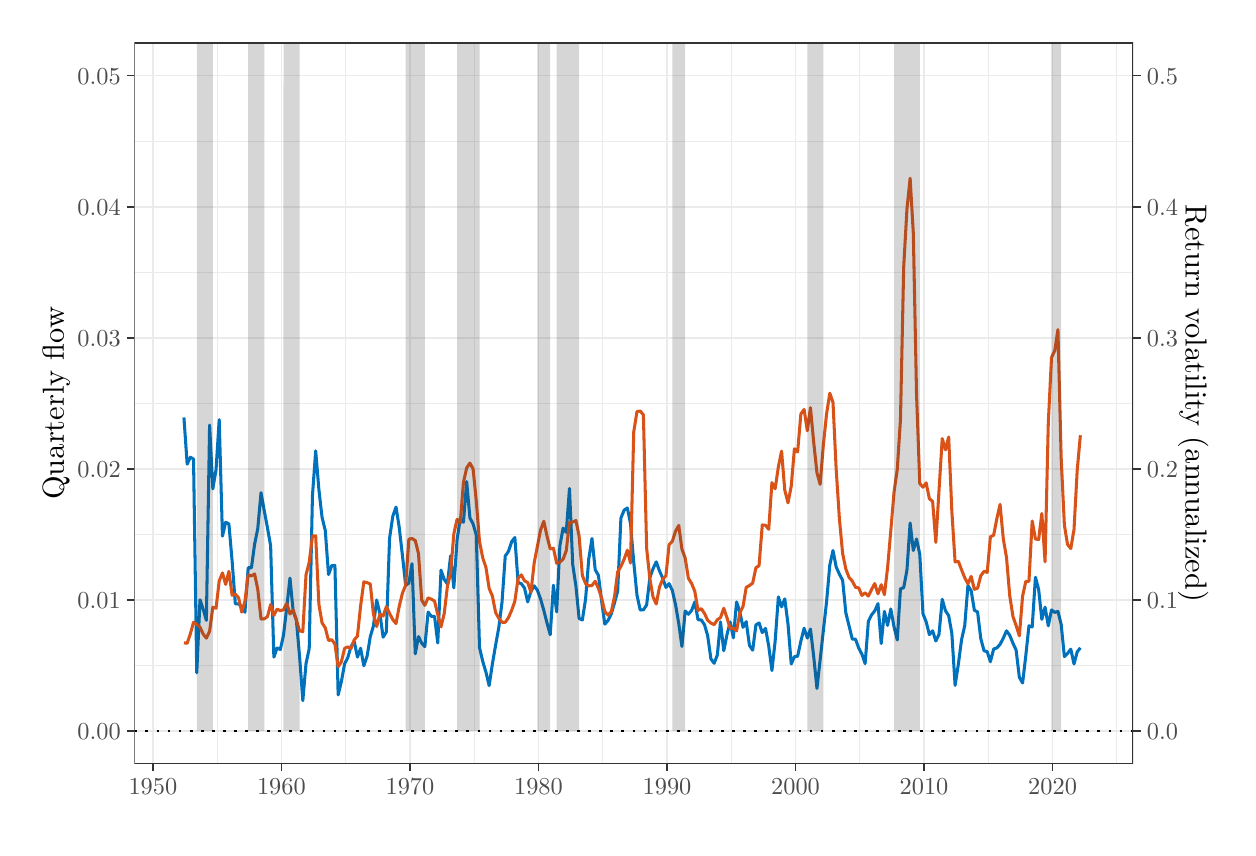
\begin{tikzpicture}[x=1pt,y=1pt]
\definecolor{fillColor}{RGB}{255,255,255}
\path[use as bounding box,fill=fillColor,fill opacity=0.00] (0,0) rectangle (433.62,289.08);
\begin{scope}
\path[clip] (  0.00,  0.00) rectangle (433.62,289.08);
\definecolor{drawColor}{RGB}{255,255,255}
\definecolor{fillColor}{RGB}{255,255,255}

\path[draw=drawColor,line width= 0.6pt,line join=round,line cap=round,fill=fillColor] (  0.00,  0.00) rectangle (433.62,289.08);
\end{scope}
\begin{scope}
\path[clip] ( 38.56, 23.11) rectangle (399.46,283.58);
\definecolor{fillColor}{RGB}{255,255,255}

\path[fill=fillColor] ( 38.56, 23.11) rectangle (399.46,283.58);
\definecolor{drawColor}{gray}{0.92}

\path[draw=drawColor,line width= 0.3pt,line join=round] ( 38.56, 58.63) --
	(399.46, 58.63);

\path[draw=drawColor,line width= 0.3pt,line join=round] ( 38.56,105.99) --
	(399.46,105.99);

\path[draw=drawColor,line width= 0.3pt,line join=round] ( 38.56,153.34) --
	(399.46,153.34);

\path[draw=drawColor,line width= 0.3pt,line join=round] ( 38.56,200.70) --
	(399.46,200.70);

\path[draw=drawColor,line width= 0.3pt,line join=round] ( 38.56,248.06) --
	(399.46,248.06);

\path[draw=drawColor,line width= 0.3pt,line join=round] ( 68.46, 23.11) --
	( 68.46,283.58);

\path[draw=drawColor,line width= 0.3pt,line join=round] (114.91, 23.11) --
	(114.91,283.58);

\path[draw=drawColor,line width= 0.3pt,line join=round] (161.35, 23.11) --
	(161.35,283.58);

\path[draw=drawColor,line width= 0.3pt,line join=round] (207.79, 23.11) --
	(207.79,283.58);

\path[draw=drawColor,line width= 0.3pt,line join=round] (254.24, 23.11) --
	(254.24,283.58);

\path[draw=drawColor,line width= 0.3pt,line join=round] (300.68, 23.11) --
	(300.68,283.58);

\path[draw=drawColor,line width= 0.3pt,line join=round] (347.13, 23.11) --
	(347.13,283.58);

\path[draw=drawColor,line width= 0.3pt,line join=round] (393.57, 23.11) --
	(393.57,283.58);

\path[draw=drawColor,line width= 0.6pt,line join=round] ( 38.56, 34.95) --
	(399.46, 34.95);

\path[draw=drawColor,line width= 0.6pt,line join=round] ( 38.56, 82.31) --
	(399.46, 82.31);

\path[draw=drawColor,line width= 0.6pt,line join=round] ( 38.56,129.67) --
	(399.46,129.67);

\path[draw=drawColor,line width= 0.6pt,line join=round] ( 38.56,177.02) --
	(399.46,177.02);

\path[draw=drawColor,line width= 0.6pt,line join=round] ( 38.56,224.38) --
	(399.46,224.38);

\path[draw=drawColor,line width= 0.6pt,line join=round] ( 38.56,271.74) --
	(399.46,271.74);

\path[draw=drawColor,line width= 0.6pt,line join=round] ( 45.24, 23.11) --
	( 45.24,283.58);

\path[draw=drawColor,line width= 0.6pt,line join=round] ( 91.68, 23.11) --
	( 91.68,283.58);

\path[draw=drawColor,line width= 0.6pt,line join=round] (138.13, 23.11) --
	(138.13,283.58);

\path[draw=drawColor,line width= 0.6pt,line join=round] (184.57, 23.11) --
	(184.57,283.58);

\path[draw=drawColor,line width= 0.6pt,line join=round] (231.02, 23.11) --
	(231.02,283.58);

\path[draw=drawColor,line width= 0.6pt,line join=round] (277.46, 23.11) --
	(277.46,283.58);

\path[draw=drawColor,line width= 0.6pt,line join=round] (323.91, 23.11) --
	(323.91,283.58);

\path[draw=drawColor,line width= 0.6pt,line join=round] (370.35, 23.11) --
	(370.35,283.58);
\definecolor{drawColor}{RGB}{0,114,189}

\path[draw=drawColor,line width= 1.1pt,line join=round] ( 56.46,148.23) --
	( 57.63,131.35) --
	( 58.78,133.87) --
	( 59.93,133.20) --
	( 61.10, 55.94) --
	( 62.27, 82.35) --
	( 63.43, 78.92) --
	( 64.57, 74.89) --
	( 65.74,145.46) --
	( 66.91,122.40) --
	( 68.07,129.42) --
	( 69.21,147.43) --
	( 70.38,105.35) --
	( 71.55,110.38) --
	( 72.71,109.76) --
	( 73.87, 96.40) --
	( 75.04, 80.86) --
	( 76.20, 80.88) --
	( 77.36, 79.88) --
	( 78.51, 77.82) --
	( 79.68, 93.93) --
	( 80.85, 93.90) --
	( 82.00,102.42) --
	( 83.15,108.14) --
	( 84.32,121.04) --
	( 85.49,114.52) --
	( 86.64,108.37) --
	( 87.79,101.91) --
	( 88.96, 61.63) --
	( 90.13, 64.95) --
	( 91.29, 64.36) --
	( 92.44, 69.56) --
	( 93.61, 79.49) --
	( 94.78, 90.18) --
	( 95.94, 78.14) --
	( 97.08, 75.12) --
	( 98.25, 61.92) --
	( 99.42, 45.90) --
	(100.58, 59.30) --
	(101.73, 64.67) --
	(102.90,119.95) --
	(104.07,136.18) --
	(105.22,122.28) --
	(106.37,112.15) --
	(107.54,107.36) --
	(108.71, 91.45) --
	(109.86, 94.67) --
	(111.02, 94.74) --
	(112.19, 47.96) --
	(113.36, 52.82) --
	(114.52, 59.22) --
	(115.66, 61.39) --
	(116.83, 65.47) --
	(118.00, 67.32) --
	(119.16, 61.64) --
	(120.30, 64.84) --
	(121.47, 58.49) --
	(122.64, 61.94) --
	(123.80, 68.99) --
	(124.94, 72.90) --
	(126.11, 82.27) --
	(127.28, 77.37) --
	(128.44, 68.83) --
	(129.60, 70.71) --
	(130.77,104.58) --
	(131.94,112.55) --
	(133.10,115.85) --
	(134.24,108.68) --
	(135.41, 98.46) --
	(136.58, 87.58) --
	(137.74, 88.39) --
	(138.88, 95.39) --
	(140.05, 62.80) --
	(141.22, 69.07) --
	(142.38, 66.67) --
	(143.52, 65.38) --
	(144.69, 77.91) --
	(145.86, 76.38) --
	(147.02, 76.35) --
	(148.18, 66.75) --
	(149.35, 93.06) --
	(150.52, 89.72) --
	(151.67, 88.05) --
	(152.82, 98.25) --
	(153.99, 86.66) --
	(155.16,104.07) --
	(156.31,111.69) --
	(157.46,110.35) --
	(158.63,125.07) --
	(159.80,111.97) --
	(160.96,109.72) --
	(162.10,105.75) --
	(163.27, 65.08) --
	(164.44, 60.06) --
	(165.60, 56.18) --
	(166.75, 51.32) --
	(167.92, 59.16) --
	(169.09, 65.97) --
	(170.25, 72.39) --
	(171.40, 81.43) --
	(172.57, 98.18) --
	(173.73, 99.82) --
	(174.89,103.34) --
	(176.04,104.86) --
	(177.21, 88.53) --
	(178.38, 88.19) --
	(179.53, 86.58) --
	(180.68, 81.58) --
	(181.85, 85.38) --
	(183.02, 87.39) --
	(184.17, 85.81) --
	(185.33, 82.66) --
	(186.50, 78.55) --
	(187.67, 73.90) --
	(188.83, 69.71) --
	(189.97, 87.62) --
	(191.14, 77.98) --
	(192.31,101.82) --
	(193.47,108.25) --
	(194.61,106.69) --
	(195.78,122.58) --
	(196.95, 95.08) --
	(198.11, 87.28) --
	(199.26, 75.61) --
	(200.43, 75.03) --
	(201.60, 82.62) --
	(202.75, 97.16) --
	(203.91,104.49) --
	(205.08, 93.21) --
	(206.25, 91.12) --
	(207.41, 81.73) --
	(208.55, 73.54) --
	(209.72, 74.87) --
	(210.89, 77.29) --
	(212.05, 81.20) --
	(213.19, 85.43) --
	(214.36,111.86) --
	(215.53,114.75) --
	(216.69,115.53) --
	(217.83,109.83) --
	(219.00, 95.94) --
	(220.17, 84.02) --
	(221.33, 78.66) --
	(222.49, 78.71) --
	(223.66, 80.48) --
	(224.83, 90.41) --
	(225.98, 93.59) --
	(227.13, 96.06) --
	(228.30, 92.78) --
	(229.47, 90.17) --
	(230.63, 86.82) --
	(231.77, 88.18) --
	(232.94, 85.72) --
	(234.11, 80.54) --
	(235.27, 73.75) --
	(236.41, 65.47) --
	(237.58, 78.29) --
	(238.75, 77.12) --
	(239.91, 78.51) --
	(241.06, 81.54) --
	(242.23, 75.15) --
	(243.40, 75.05) --
	(244.56, 73.36) --
	(245.71, 69.40) --
	(246.88, 61.00) --
	(248.05, 59.40) --
	(249.20, 62.36) --
	(250.35, 74.36) --
	(251.52, 63.92) --
	(252.69, 69.71) --
	(253.84, 74.34) --
	(254.99, 68.59) --
	(256.16, 81.58) --
	(257.33, 77.98) --
	(258.49, 72.40) --
	(259.64, 74.44) --
	(260.81, 65.85) --
	(261.98, 64.13) --
	(263.14, 73.26) --
	(264.28, 73.98) --
	(265.45, 70.49) --
	(266.62, 72.03) --
	(267.78, 65.60) --
	(268.93, 56.78) --
	(270.10, 67.42) --
	(271.26, 83.40) --
	(272.42, 79.82) --
	(273.57, 82.68) --
	(274.74, 73.61) --
	(275.91, 59.14) --
	(277.06, 61.79) --
	(278.22, 61.96) --
	(279.39, 67.39) --
	(280.56, 72.08) --
	(281.72, 68.52) --
	(282.86, 71.76) --
	(284.03, 61.85) --
	(285.20, 50.31) --
	(286.36, 60.66) --
	(287.50, 71.10) --
	(288.67, 81.53) --
	(289.84, 94.91) --
	(291.00,100.15) --
	(292.14, 94.25) --
	(293.31, 91.60) --
	(294.48, 89.41) --
	(295.64, 77.63) --
	(296.80, 72.95) --
	(297.97, 68.14) --
	(299.14, 68.10) --
	(300.30, 64.88) --
	(301.44, 62.72) --
	(302.61, 59.25) --
	(303.78, 74.55) --
	(304.94, 76.89) --
	(306.08, 78.32) --
	(307.25, 80.95) --
	(308.42, 66.52) --
	(309.58, 78.17) --
	(310.72, 73.09) --
	(311.89, 79.03) --
	(313.06, 72.53) --
	(314.22, 67.82) --
	(315.38, 86.32) --
	(316.55, 86.73) --
	(317.72, 93.05) --
	(318.87,110.10) --
	(320.02,100.16) --
	(321.19,104.32) --
	(322.36, 98.80) --
	(323.51, 77.33) --
	(324.66, 74.39) --
	(325.83, 69.74) --
	(327.00, 71.15) --
	(328.16, 67.46) --
	(329.30, 69.85) --
	(330.47, 82.54) --
	(331.64, 78.38) --
	(332.80, 76.60) --
	(333.95, 70.19) --
	(335.12, 51.40) --
	(336.29, 59.02) --
	(337.45, 67.88) --
	(338.60, 72.98) --
	(339.76, 87.52) --
	(340.93, 85.63) --
	(342.09, 78.53) --
	(343.24, 77.98) --
	(344.41, 68.27) --
	(345.58, 63.96) --
	(346.73, 63.57) --
	(347.88, 59.95) --
	(349.05, 64.56) --
	(350.22, 64.98) --
	(351.37, 66.23) --
	(352.53, 68.46) --
	(353.70, 71.13) --
	(354.87, 69.50) --
	(356.03, 66.65) --
	(357.17, 64.18) --
	(358.34, 54.32) --
	(359.51, 52.28) --
	(360.67, 62.19) --
	(361.81, 72.94) --
	(362.98, 72.51) --
	(364.15, 90.49) --
	(365.31, 86.11) --
	(366.46, 75.25) --
	(367.63, 79.68) --
	(368.80, 72.94) --
	(369.95, 78.69) --
	(371.11, 77.80) --
	(372.28, 78.14) --
	(373.45, 73.51) --
	(374.61, 61.79) --
	(375.75, 62.97) --
	(376.92, 64.51) --
	(378.09, 59.15) --
	(379.25, 63.53) --
	(380.39, 65.00);
\definecolor{drawColor}{RGB}{217,83,25}

\path[draw=drawColor,line width= 1.1pt,line join=round] ( 56.46, 66.79) --
	( 57.63, 66.63) --
	( 58.78, 70.01) --
	( 59.93, 74.24) --
	( 61.10, 73.46) --
	( 62.27, 72.45) --
	( 63.43, 69.92) --
	( 64.57, 68.49) --
	( 65.74, 70.98) --
	( 66.91, 79.67) --
	( 68.07, 79.29) --
	( 69.21, 89.14) --
	( 70.38, 92.05) --
	( 71.55, 87.89) --
	( 72.71, 92.64) --
	( 73.87, 84.00) --
	( 75.04, 84.38) --
	( 76.20, 83.09) --
	( 77.36, 77.90) --
	( 78.51, 81.82) --
	( 79.68, 91.35) --
	( 80.85, 90.96) --
	( 82.00, 91.70) --
	( 83.15, 86.06) --
	( 84.32, 75.39) --
	( 85.49, 75.45) --
	( 86.64, 76.25) --
	( 87.79, 80.63) --
	( 88.96, 76.66) --
	( 90.13, 78.98) --
	( 91.29, 78.40) --
	( 92.44, 78.75) --
	( 93.61, 81.06) --
	( 94.78, 77.21) --
	( 95.94, 78.67) --
	( 97.08, 74.98) --
	( 98.25, 71.08) --
	( 99.42, 70.85) --
	(100.58, 91.38) --
	(101.73, 95.84) --
	(102.90,105.40) --
	(104.07,105.47) --
	(105.22, 80.76) --
	(106.37, 74.04) --
	(107.54, 72.19) --
	(108.71, 67.64) --
	(109.86, 67.92) --
	(111.02, 66.37) --
	(112.19, 58.11) --
	(113.36, 59.95) --
	(114.52, 64.81) --
	(115.66, 65.33) --
	(116.83, 64.75) --
	(118.00, 67.89) --
	(119.16, 69.21) --
	(120.30, 80.08) --
	(121.47, 88.83) --
	(122.64, 88.53) --
	(123.80, 88.06) --
	(124.94, 77.14) --
	(126.11, 72.68) --
	(127.28, 77.15) --
	(128.44, 76.49) --
	(129.60, 79.88) --
	(130.77, 77.45) --
	(131.94, 75.16) --
	(133.10, 73.75) --
	(134.24, 79.88) --
	(135.41, 84.72) --
	(136.58, 87.65) --
	(137.74,104.26) --
	(138.88,104.48) --
	(140.05,103.77) --
	(141.22, 99.06) --
	(142.38, 82.25) --
	(143.52, 80.33) --
	(144.69, 83.03) --
	(145.86, 82.59) --
	(147.02, 81.88) --
	(148.18, 77.04) --
	(149.35, 72.54) --
	(150.52, 77.41) --
	(151.67, 87.21) --
	(152.82, 91.97) --
	(153.99,106.16) --
	(155.16,111.43) --
	(156.31,110.05) --
	(157.46,124.74) --
	(158.63,130.00) --
	(159.80,131.73) --
	(160.96,129.62) --
	(162.10,118.01) --
	(163.27,103.44) --
	(164.44, 97.48) --
	(165.60, 93.99) --
	(166.75, 86.47) --
	(167.92, 83.69) --
	(169.09, 77.73) --
	(170.25, 75.65) --
	(171.40, 74.24) --
	(172.57, 74.19) --
	(173.73, 75.89) --
	(174.89, 78.55) --
	(176.04, 81.81) --
	(177.21, 90.12) --
	(178.38, 91.36) --
	(179.53, 89.21) --
	(180.68, 88.59) --
	(181.85, 85.09) --
	(183.02, 95.64) --
	(184.17,101.64) --
	(185.33,107.56) --
	(186.50,110.74) --
	(187.67,105.31) --
	(188.83,100.72) --
	(189.97,100.99) --
	(191.14, 95.56) --
	(192.31, 95.98) --
	(193.47, 97.02) --
	(194.61,100.06) --
	(195.78,110.33) --
	(196.95,110.46) --
	(198.11,110.97) --
	(199.26,105.40) --
	(200.43, 91.12) --
	(201.60, 88.19) --
	(202.75, 87.35) --
	(203.91, 87.51) --
	(205.08, 89.04) --
	(206.25, 86.42) --
	(207.41, 82.96) --
	(208.55, 78.08) --
	(209.72, 76.80) --
	(210.89, 78.06) --
	(212.05, 83.47) --
	(213.19, 92.44) --
	(214.36, 94.36) --
	(215.53, 97.03) --
	(216.69,100.26) --
	(217.83, 95.62) --
	(219.00,143.01) --
	(220.17,150.37) --
	(221.33,150.55) --
	(222.49,149.16) --
	(223.66,100.92) --
	(224.83, 89.92) --
	(225.98, 83.33) --
	(227.13, 80.82) --
	(228.30, 86.93) --
	(229.47, 89.78) --
	(230.63, 91.01) --
	(231.77,102.25) --
	(232.94,103.50) --
	(234.11,107.13) --
	(235.27,109.20) --
	(236.41,100.63) --
	(237.58, 97.48) --
	(238.75, 90.11) --
	(239.91, 88.22) --
	(241.06, 85.41) --
	(242.23, 78.50) --
	(243.40, 79.15) --
	(244.56, 77.44) --
	(245.71, 74.96) --
	(246.88, 73.94) --
	(248.05, 73.35) --
	(249.20, 75.13) --
	(250.35, 75.89) --
	(251.52, 79.28) --
	(252.69, 75.87) --
	(253.84, 71.99) --
	(254.99, 72.13) --
	(256.16, 71.11) --
	(257.33, 77.64) --
	(258.49, 79.92) --
	(259.64, 86.85) --
	(260.81, 87.49) --
	(261.98, 88.38) --
	(263.14, 93.90) --
	(264.28, 94.67) --
	(265.45,109.38) --
	(266.62,109.28) --
	(267.78,107.81) --
	(268.93,124.69) --
	(270.10,122.46) --
	(271.26,130.41) --
	(272.42,136.06) --
	(273.57,121.99) --
	(274.74,117.36) --
	(275.91,123.39) --
	(277.06,136.92) --
	(278.22,135.75) --
	(279.39,149.50) --
	(280.56,151.12) --
	(281.72,143.42) --
	(282.86,151.77) --
	(284.03,139.22) --
	(285.20,128.25) --
	(286.36,124.05) --
	(287.50,138.10) --
	(288.67,149.44) --
	(289.84,156.99) --
	(291.00,153.66) --
	(292.14,129.69) --
	(293.31,111.68) --
	(294.48, 99.09) --
	(295.64, 93.48) --
	(296.80, 90.43) --
	(297.97, 89.10) --
	(299.14, 86.85) --
	(300.30, 86.64) --
	(301.44, 83.92) --
	(302.61, 84.86) --
	(303.78, 83.68) --
	(304.94, 86.08) --
	(306.08, 88.22) --
	(307.25, 84.50) --
	(308.42, 87.78) --
	(309.58, 84.18) --
	(310.72, 93.87) --
	(311.89,107.32) --
	(313.06,121.37) --
	(314.22,129.43) --
	(315.38,147.40) --
	(316.55,202.67) --
	(317.72,223.49) --
	(318.87,234.68) --
	(320.02,214.83) --
	(321.19,156.57) --
	(322.36,124.36) --
	(323.51,123.02) --
	(324.66,124.58) --
	(325.83,118.87) --
	(327.00,117.90) --
	(328.16,103.08) --
	(329.30,121.67) --
	(330.47,140.60) --
	(331.64,136.53) --
	(332.80,141.16) --
	(333.95,114.22) --
	(335.12, 96.02) --
	(336.29, 96.26) --
	(337.45, 93.20) --
	(338.60, 90.33) --
	(339.76, 88.12) --
	(340.93, 90.80) --
	(342.09, 86.12) --
	(343.24, 86.53) --
	(344.41, 91.01) --
	(345.58, 92.63) --
	(346.73, 92.25) --
	(347.88,105.13) --
	(349.05,105.65) --
	(350.22,111.74) --
	(351.37,116.80) --
	(352.53,104.47) --
	(353.70, 97.60) --
	(354.87, 83.78) --
	(356.03, 76.28) --
	(357.17, 73.03) --
	(358.34, 69.30) --
	(359.51, 83.68) --
	(360.67, 89.00) --
	(361.81, 89.02) --
	(362.98,110.84) --
	(364.15,104.33) --
	(365.31,104.12) --
	(366.46,113.54) --
	(367.63, 96.07) --
	(368.80,146.28) --
	(369.95,169.89) --
	(371.11,172.32) --
	(372.28,179.97) --
	(373.45,133.71) --
	(374.61,109.32) --
	(375.75,102.33) --
	(376.92,100.85) --
	(378.09,107.76) --
	(379.25,129.21) --
	(380.39,141.80);
\definecolor{fillColor}{RGB}{51,51,51}

\path[fill=fillColor,fill opacity=0.20] ( 55.29, 34.95) --
	( 55.61, 34.95) --
	( 56.13, 34.95) --
	( 56.46, 34.95) --
	( 56.78, 34.95) --
	( 57.30, 34.95) --
	( 57.63, 34.95) --
	( 57.95, 34.95) --
	( 58.46, 34.95) --
	( 58.78, 34.95) --
	( 59.11, 34.95) --
	( 59.60, 34.95) --
	( 59.93, 34.95) --
	( 60.26, 34.95) --
	( 60.77, 34.95) --
	( 61.10, 34.95) --
	( 61.10,2023.56) --
	( 66.90,2023.56) --
	( 66.91, 34.95) --
	( 67.24, 34.95) --
	( 67.74, 34.95) --
	( 68.07, 34.95) --
	( 68.39, 34.95) --
	( 68.88, 34.95) --
	( 69.21, 34.95) --
	( 69.54, 34.95) --
	( 70.05, 34.95) --
	( 70.38, 34.95) --
	( 70.71, 34.95) --
	( 71.22, 34.95) --
	( 71.55, 34.95) --
	( 71.88, 34.95) --
	( 72.38, 34.95) --
	( 72.71, 34.95) --
	( 73.04, 34.95) --
	( 73.54, 34.95) --
	( 73.87, 34.95) --
	( 74.19, 34.95) --
	( 74.71, 34.95) --
	( 75.04, 34.95) --
	( 75.36, 34.95) --
	( 75.88, 34.95) --
	( 76.20, 34.95) --
	( 76.53, 34.95) --
	( 77.03, 34.95) --
	( 77.36, 34.95) --
	( 77.69, 34.95) --
	( 78.18, 34.95) --
	( 78.51, 34.95) --
	( 78.83, 34.95) --
	( 79.35, 34.95) --
	( 79.68, 34.95) --
	( 79.68,2023.56) --
	( 85.48,2023.56) --
	( 85.49, 34.95) --
	( 85.81, 34.95) --
	( 86.32, 34.95) --
	( 86.64, 34.95) --
	( 86.97, 34.95) --
	( 87.46, 34.95) --
	( 87.79, 34.95) --
	( 88.12, 34.95) --
	( 88.63, 34.95) --
	( 88.96, 34.95) --
	( 89.29, 34.95) --
	( 89.80, 34.95) --
	( 90.13, 34.95) --
	( 90.46, 34.95) --
	( 90.96, 34.95) --
	( 91.29, 34.95) --
	( 91.61, 34.95) --
	( 92.12, 34.95) --
	( 92.44, 34.95) --
	( 92.45,2023.56) --
	( 98.25,2023.56) --
	( 98.25, 34.95) --
	( 98.58, 34.95) --
	( 99.10, 34.95) --
	( 99.42, 34.95) --
	( 99.75, 34.95) --
	(100.25, 34.95) --
	(100.58, 34.95) --
	(100.91, 34.95) --
	(101.40, 34.95) --
	(101.73, 34.95) --
	(102.05, 34.95) --
	(102.57, 34.95) --
	(102.90, 34.95) --
	(103.22, 34.95) --
	(103.74, 34.95) --
	(104.07, 34.95) --
	(104.39, 34.95) --
	(104.89, 34.95) --
	(105.22, 34.95) --
	(105.55, 34.95) --
	(106.04, 34.95) --
	(106.37, 34.95) --
	(106.69, 34.95) --
	(107.21, 34.95) --
	(107.54, 34.95) --
	(107.86, 34.95) --
	(108.38, 34.95) --
	(108.71, 34.95) --
	(109.03, 34.95) --
	(109.54, 34.95) --
	(109.86, 34.95) --
	(110.19, 34.95) --
	(110.69, 34.95) --
	(111.02, 34.95) --
	(111.35, 34.95) --
	(111.86, 34.95) --
	(112.19, 34.95) --
	(112.52, 34.95) --
	(113.03, 34.95) --
	(113.36, 34.95) --
	(113.69, 34.95) --
	(114.19, 34.95) --
	(114.52, 34.95) --
	(114.84, 34.95) --
	(115.33, 34.95) --
	(115.66, 34.95) --
	(115.99, 34.95) --
	(116.50, 34.95) --
	(116.83, 34.95) --
	(117.16, 34.95) --
	(117.67, 34.95) --
	(118.00, 34.95) --
	(118.33, 34.95) --
	(118.83, 34.95) --
	(119.16, 34.95) --
	(119.49, 34.95) --
	(119.98, 34.95) --
	(120.30, 34.95) --
	(120.63, 34.95) --
	(121.15, 34.95) --
	(121.47, 34.95) --
	(121.80, 34.95) --
	(122.32, 34.95) --
	(122.64, 34.95) --
	(122.97, 34.95) --
	(123.47, 34.95) --
	(123.80, 34.95) --
	(124.13, 34.95) --
	(124.62, 34.95) --
	(124.94, 34.95) --
	(125.27, 34.95) --
	(125.79, 34.95) --
	(126.11, 34.95) --
	(126.44, 34.95) --
	(126.96, 34.95) --
	(127.28, 34.95) --
	(127.61, 34.95) --
	(128.11, 34.95) --
	(128.44, 34.95) --
	(128.77, 34.95) --
	(129.27, 34.95) --
	(129.60, 34.95) --
	(129.93, 34.95) --
	(130.44, 34.95) --
	(130.77, 34.95) --
	(131.10, 34.95) --
	(131.61, 34.95) --
	(131.94, 34.95) --
	(132.27, 34.95) --
	(132.77, 34.95) --
	(133.10, 34.95) --
	(133.42, 34.95) --
	(133.91, 34.95) --
	(134.24, 34.95) --
	(134.57, 34.95) --
	(135.08, 34.95) --
	(135.41, 34.95) --
	(135.74, 34.95) --
	(136.25, 34.95) --
	(136.58, 34.95) --
	(136.58,2023.56) --
	(143.52,2023.56) --
	(143.52, 34.95) --
	(143.85, 34.95) --
	(144.36, 34.95) --
	(144.69, 34.95) --
	(145.02, 34.95) --
	(145.53, 34.95) --
	(145.86, 34.95) --
	(146.19, 34.95) --
	(146.69, 34.95) --
	(147.02, 34.95) --
	(147.35, 34.95) --
	(147.85, 34.95) --
	(148.18, 34.95) --
	(148.50, 34.95) --
	(149.02, 34.95) --
	(149.35, 34.95) --
	(149.67, 34.95) --
	(150.19, 34.95) --
	(150.52, 34.95) --
	(150.84, 34.95) --
	(151.35, 34.95) --
	(151.67, 34.95) --
	(152.00, 34.95) --
	(152.49, 34.95) --
	(152.82, 34.95) --
	(153.14, 34.95) --
	(153.66, 34.95) --
	(153.99, 34.95) --
	(154.31, 34.95) --
	(154.83, 34.95) --
	(155.16, 34.95) --
	(155.16,2023.56) --
	(163.26,2023.56) --
	(163.27, 34.95) --
	(163.60, 34.95) --
	(164.11, 34.95) --
	(164.44, 34.95) --
	(164.77, 34.95) --
	(165.27, 34.95) --
	(165.60, 34.95) --
	(165.92, 34.95) --
	(166.43, 34.95) --
	(166.75, 34.95) --
	(167.08, 34.95) --
	(167.60, 34.95) --
	(167.92, 34.95) --
	(168.25, 34.95) --
	(168.77, 34.95) --
	(169.09, 34.95) --
	(169.42, 34.95) --
	(169.92, 34.95) --
	(170.25, 34.95) --
	(170.58, 34.95) --
	(171.07, 34.95) --
	(171.40, 34.95) --
	(171.72, 34.95) --
	(172.24, 34.95) --
	(172.57, 34.95) --
	(172.89, 34.95) --
	(173.41, 34.95) --
	(173.73, 34.95) --
	(174.06, 34.95) --
	(174.56, 34.95) --
	(174.89, 34.95) --
	(175.22, 34.95) --
	(175.71, 34.95) --
	(176.04, 34.95) --
	(176.36, 34.95) --
	(176.88, 34.95) --
	(177.21, 34.95) --
	(177.53, 34.95) --
	(178.05, 34.95) --
	(178.38, 34.95) --
	(178.70, 34.95) --
	(179.21, 34.95) --
	(179.53, 34.95) --
	(179.86, 34.95) --
	(180.35, 34.95) --
	(180.68, 34.95) --
	(181.01, 34.95) --
	(181.52, 34.95) --
	(181.85, 34.95) --
	(182.18, 34.95) --
	(182.69, 34.95) --
	(183.02, 34.95) --
	(183.34, 34.95) --
	(183.85, 34.95) --
	(184.17, 34.95) --
	(184.18,2023.56) --
	(188.82,2023.56) --
	(188.83, 34.95) --
	(189.16, 34.95) --
	(189.65, 34.95) --
	(189.97, 34.95) --
	(190.30, 34.95) --
	(190.82, 34.95) --
	(191.14, 34.95) --
	(191.15,2023.56) --
	(199.25,2023.56) --
	(199.26, 34.95) --
	(199.58, 34.95) --
	(200.10, 34.95) --
	(200.43, 34.95) --
	(200.75, 34.95) --
	(201.27, 34.95) --
	(201.60, 34.95) --
	(201.92, 34.95) --
	(202.42, 34.95) --
	(202.75, 34.95) --
	(203.08, 34.95) --
	(203.58, 34.95) --
	(203.91, 34.95) --
	(204.24, 34.95) --
	(204.75, 34.95) --
	(205.08, 34.95) --
	(205.41, 34.95) --
	(205.92, 34.95) --
	(206.25, 34.95) --
	(206.58, 34.95) --
	(207.08, 34.95) --
	(207.41, 34.95) --
	(207.73, 34.95) --
	(208.22, 34.95) --
	(208.55, 34.95) --
	(208.88, 34.95) --
	(209.39, 34.95) --
	(209.72, 34.95) --
	(210.05, 34.95) --
	(210.56, 34.95) --
	(210.89, 34.95) --
	(211.22, 34.95) --
	(211.72, 34.95) --
	(212.05, 34.95) --
	(212.38, 34.95) --
	(212.86, 34.95) --
	(213.19, 34.95) --
	(213.52, 34.95) --
	(214.03, 34.95) --
	(214.36, 34.95) --
	(214.69, 34.95) --
	(215.20, 34.95) --
	(215.53, 34.95) --
	(215.86, 34.95) --
	(216.36, 34.95) --
	(216.69, 34.95) --
	(217.02, 34.95) --
	(217.51, 34.95) --
	(217.83, 34.95) --
	(218.16, 34.95) --
	(218.68, 34.95) --
	(219.00, 34.95) --
	(219.33, 34.95) --
	(219.85, 34.95) --
	(220.17, 34.95) --
	(220.50, 34.95) --
	(221.00, 34.95) --
	(221.33, 34.95) --
	(221.66, 34.95) --
	(222.16, 34.95) --
	(222.49, 34.95) --
	(222.81, 34.95) --
	(223.33, 34.95) --
	(223.66, 34.95) --
	(223.98, 34.95) --
	(224.50, 34.95) --
	(224.83, 34.95) --
	(225.15, 34.95) --
	(225.66, 34.95) --
	(225.98, 34.95) --
	(226.31, 34.95) --
	(226.80, 34.95) --
	(227.13, 34.95) --
	(227.46, 34.95) --
	(227.97, 34.95) --
	(228.30, 34.95) --
	(228.63, 34.95) --
	(229.14, 34.95) --
	(229.47, 34.95) --
	(229.80, 34.95) --
	(230.30, 34.95) --
	(230.63, 34.95) --
	(230.95, 34.95) --
	(231.44, 34.95) --
	(231.77, 34.95) --
	(232.10, 34.95) --
	(232.61, 34.95) --
	(232.94, 34.95) --
	(232.94,2023.56) --
	(237.58,2023.56) --
	(237.58, 34.95) --
	(237.91, 34.95) --
	(238.42, 34.95) --
	(238.75, 34.95) --
	(239.08, 34.95) --
	(239.58, 34.95) --
	(239.91, 34.95) --
	(240.24, 34.95) --
	(240.74, 34.95) --
	(241.06, 34.95) --
	(241.39, 34.95) --
	(241.91, 34.95) --
	(242.23, 34.95) --
	(242.56, 34.95) --
	(243.08, 34.95) --
	(243.40, 34.95) --
	(243.73, 34.95) --
	(244.23, 34.95) --
	(244.56, 34.95) --
	(244.89, 34.95) --
	(245.38, 34.95) --
	(245.71, 34.95) --
	(246.03, 34.95) --
	(246.55, 34.95) --
	(246.88, 34.95) --
	(247.20, 34.95) --
	(247.72, 34.95) --
	(248.05, 34.95) --
	(248.37, 34.95) --
	(248.88, 34.95) --
	(249.20, 34.95) --
	(249.53, 34.95) --
	(250.02, 34.95) --
	(250.35, 34.95) --
	(250.67, 34.95) --
	(251.19, 34.95) --
	(251.52, 34.95) --
	(251.84, 34.95) --
	(252.36, 34.95) --
	(252.69, 34.95) --
	(253.01, 34.95) --
	(253.52, 34.95) --
	(253.84, 34.95) --
	(254.17, 34.95) --
	(254.66, 34.95) --
	(254.99, 34.95) --
	(255.32, 34.95) --
	(255.83, 34.95) --
	(256.16, 34.95) --
	(256.49, 34.95) --
	(257.00, 34.95) --
	(257.33, 34.95) --
	(257.66, 34.95) --
	(258.16, 34.95) --
	(258.49, 34.95) --
	(258.81, 34.95) --
	(259.32, 34.95) --
	(259.64, 34.95) --
	(259.97, 34.95) --
	(260.49, 34.95) --
	(260.81, 34.95) --
	(261.14, 34.95) --
	(261.66, 34.95) --
	(261.98, 34.95) --
	(262.31, 34.95) --
	(262.81, 34.95) --
	(263.14, 34.95) --
	(263.47, 34.95) --
	(263.96, 34.95) --
	(264.28, 34.95) --
	(264.61, 34.95) --
	(265.13, 34.95) --
	(265.45, 34.95) --
	(265.78, 34.95) --
	(266.30, 34.95) --
	(266.62, 34.95) --
	(266.95, 34.95) --
	(267.45, 34.95) --
	(267.78, 34.95) --
	(268.11, 34.95) --
	(268.60, 34.95) --
	(268.93, 34.95) --
	(269.25, 34.95) --
	(269.77, 34.95) --
	(270.10, 34.95) --
	(270.42, 34.95) --
	(270.94, 34.95) --
	(271.26, 34.95) --
	(271.59, 34.95) --
	(272.09, 34.95) --
	(272.42, 34.95) --
	(272.75, 34.95) --
	(273.24, 34.95) --
	(273.57, 34.95) --
	(273.89, 34.95) --
	(274.41, 34.95) --
	(274.74, 34.95) --
	(275.06, 34.95) --
	(275.58, 34.95) --
	(275.91, 34.95) --
	(276.23, 34.95) --
	(276.74, 34.95) --
	(277.06, 34.95) --
	(277.39, 34.95) --
	(277.89, 34.95) --
	(278.22, 34.95) --
	(278.55, 34.95) --
	(279.06, 34.95) --
	(279.39, 34.95) --
	(279.72, 34.95) --
	(280.23, 34.95) --
	(280.56, 34.95) --
	(280.89, 34.95) --
	(281.39, 34.95) --
	(281.72, 34.95) --
	(281.72,2023.56) --
	(287.50,2023.56) --
	(287.50, 34.95) --
	(287.83, 34.95) --
	(288.35, 34.95) --
	(288.67, 34.95) --
	(289.00, 34.95) --
	(289.52, 34.95) --
	(289.84, 34.95) --
	(290.17, 34.95) --
	(290.67, 34.95) --
	(291.00, 34.95) --
	(291.33, 34.95) --
	(291.82, 34.95) --
	(292.14, 34.95) --
	(292.47, 34.95) --
	(292.99, 34.95) --
	(293.31, 34.95) --
	(293.64, 34.95) --
	(294.16, 34.95) --
	(294.48, 34.95) --
	(294.81, 34.95) --
	(295.31, 34.95) --
	(295.64, 34.95) --
	(295.97, 34.95) --
	(296.47, 34.95) --
	(296.80, 34.95) --
	(297.13, 34.95) --
	(297.64, 34.95) --
	(297.97, 34.95) --
	(298.30, 34.95) --
	(298.81, 34.95) --
	(299.14, 34.95) --
	(299.47, 34.95) --
	(299.97, 34.95) --
	(300.30, 34.95) --
	(300.62, 34.95) --
	(301.11, 34.95) --
	(301.44, 34.95) --
	(301.77, 34.95) --
	(302.28, 34.95) --
	(302.61, 34.95) --
	(302.94, 34.95) --
	(303.45, 34.95) --
	(303.78, 34.95) --
	(304.11, 34.95) --
	(304.61, 34.95) --
	(304.94, 34.95) --
	(305.26, 34.95) --
	(305.75, 34.95) --
	(306.08, 34.95) --
	(306.41, 34.95) --
	(306.92, 34.95) --
	(307.25, 34.95) --
	(307.58, 34.95) --
	(308.09, 34.95) --
	(308.42, 34.95) --
	(308.75, 34.95) --
	(309.25, 34.95) --
	(309.58, 34.95) --
	(309.91, 34.95) --
	(310.39, 34.95) --
	(310.72, 34.95) --
	(311.05, 34.95) --
	(311.56, 34.95) --
	(311.89, 34.95) --
	(312.22, 34.95) --
	(312.73, 34.95) --
	(313.06, 34.95) --
	(313.07,2023.56) --
	(322.35,2023.56) --
	(322.36, 34.95) --
	(322.68, 34.95) --
	(323.19, 34.95) --
	(323.51, 34.95) --
	(323.84, 34.95) --
	(324.33, 34.95) --
	(324.66, 34.95) --
	(324.99, 34.95) --
	(325.50, 34.95) --
	(325.83, 34.95) --
	(326.16, 34.95) --
	(326.67, 34.95) --
	(327.00, 34.95) --
	(327.33, 34.95) --
	(327.83, 34.95) --
	(328.16, 34.95) --
	(328.48, 34.95) --
	(328.97, 34.95) --
	(329.30, 34.95) --
	(329.63, 34.95) --
	(330.14, 34.95) --
	(330.47, 34.95) --
	(330.80, 34.95) --
	(331.31, 34.95) --
	(331.64, 34.95) --
	(331.97, 34.95) --
	(332.47, 34.95) --
	(332.80, 34.95) --
	(333.12, 34.95) --
	(333.63, 34.95) --
	(333.95, 34.95) --
	(334.28, 34.95) --
	(334.80, 34.95) --
	(335.12, 34.95) --
	(335.45, 34.95) --
	(335.97, 34.95) --
	(336.29, 34.95) --
	(336.62, 34.95) --
	(337.12, 34.95) --
	(337.45, 34.95) --
	(337.78, 34.95) --
	(338.27, 34.95) --
	(338.60, 34.95) --
	(338.92, 34.95) --
	(339.44, 34.95) --
	(339.76, 34.95) --
	(340.09, 34.95) --
	(340.61, 34.95) --
	(340.93, 34.95) --
	(341.26, 34.95) --
	(341.76, 34.95) --
	(342.09, 34.95) --
	(342.42, 34.95) --
	(342.91, 34.95) --
	(343.24, 34.95) --
	(343.56, 34.95) --
	(344.08, 34.95) --
	(344.41, 34.95) --
	(344.73, 34.95) --
	(345.25, 34.95) --
	(345.58, 34.95) --
	(345.90, 34.95) --
	(346.41, 34.95) --
	(346.73, 34.95) --
	(347.06, 34.95) --
	(347.55, 34.95) --
	(347.88, 34.95) --
	(348.21, 34.95) --
	(348.72, 34.95) --
	(349.05, 34.95) --
	(349.37, 34.95) --
	(349.89, 34.95) --
	(350.22, 34.95) --
	(350.54, 34.95) --
	(351.05, 34.95) --
	(351.37, 34.95) --
	(351.70, 34.95) --
	(352.20, 34.95) --
	(352.53, 34.95) --
	(352.86, 34.95) --
	(353.37, 34.95) --
	(353.70, 34.95) --
	(354.03, 34.95) --
	(354.54, 34.95) --
	(354.87, 34.95) --
	(355.20, 34.95) --
	(355.70, 34.95) --
	(356.03, 34.95) --
	(356.36, 34.95) --
	(356.85, 34.95) --
	(357.17, 34.95) --
	(357.50, 34.95) --
	(358.02, 34.95) --
	(358.34, 34.95) --
	(358.67, 34.95) --
	(359.19, 34.95) --
	(359.51, 34.95) --
	(359.84, 34.95) --
	(360.34, 34.95) --
	(360.67, 34.95) --
	(361.00, 34.95) --
	(361.49, 34.95) --
	(361.81, 34.95) --
	(362.14, 34.95) --
	(362.66, 34.95) --
	(362.98, 34.95) --
	(363.31, 34.95) --
	(363.83, 34.95) --
	(364.15, 34.95) --
	(364.48, 34.95) --
	(364.98, 34.95) --
	(365.31, 34.95) --
	(365.64, 34.95) --
	(366.13, 34.95) --
	(366.46, 34.95) --
	(366.78, 34.95) --
	(367.30, 34.95) --
	(367.63, 34.95) --
	(367.95, 34.95) --
	(368.47, 34.95) --
	(368.80, 34.95) --
	(369.12, 34.95) --
	(369.62, 34.95) --
	(369.95, 34.95) --
	(369.96,2023.56) --
	(373.44,2023.56) --
	(373.45, 34.95) --
	(373.78, 34.95) --
	(374.28, 34.95) --
	(374.61, 34.95) --
	(374.93, 34.95) --
	(375.42, 34.95) --
	(375.75, 34.95) --
	(376.08, 34.95) --
	(376.59, 34.95) --
	(376.92, 34.95) --
	(377.25, 34.95) --
	(377.76, 34.95) --
	(378.09, 34.95) --
	(378.42, 34.95) --
	(378.92, 34.95) --
	(379.25, 34.95) --
	(379.57, 34.95) --
	(380.06, 34.95) --
	(380.39, 34.95) --
	(380.72, 34.95) --
	(381.23, 34.95) --
	(381.56, 34.95) --
	(381.89, 34.95) --
	(382.40, 34.95) --
	(382.73, 34.95) --
	(383.06, 34.95) --
	(382.73, 34.95) --
	(382.40, 34.95) --
	(381.89, 34.95) --
	(381.56, 34.95) --
	(381.23, 34.95) --
	(380.72, 34.95) --
	(380.39, 34.95) --
	(380.06, 34.95) --
	(379.57, 34.95) --
	(379.25, 34.95) --
	(378.92, 34.95) --
	(378.42, 34.95) --
	(378.09, 34.95) --
	(377.76, 34.95) --
	(377.25, 34.95) --
	(376.92, 34.95) --
	(376.59, 34.95) --
	(376.08, 34.95) --
	(375.75, 34.95) --
	(375.42, 34.95) --
	(374.93, 34.95) --
	(374.61, 34.95) --
	(374.28, 34.95) --
	(373.78, 34.95) --
	(373.45, 34.95) --
	(373.12, 34.95) --
	(372.61, 34.95) --
	(372.28, 34.95) --
	(371.95, 34.95) --
	(371.44, 34.95) --
	(371.11, 34.95) --
	(370.78, 34.95) --
	(370.28, 34.95) --
	(369.95, 34.95) --
	(369.62, 34.95) --
	(369.12, 34.95) --
	(368.80, 34.95) --
	(368.47, 34.95) --
	(367.95, 34.95) --
	(367.63, 34.95) --
	(367.30, 34.95) --
	(366.78, 34.95) --
	(366.46, 34.95) --
	(366.13, 34.95) --
	(365.64, 34.95) --
	(365.31, 34.95) --
	(364.98, 34.95) --
	(364.48, 34.95) --
	(364.15, 34.95) --
	(363.83, 34.95) --
	(363.31, 34.95) --
	(362.98, 34.95) --
	(362.66, 34.95) --
	(362.14, 34.95) --
	(361.81, 34.95) --
	(361.49, 34.95) --
	(361.00, 34.95) --
	(360.67, 34.95) --
	(360.34, 34.95) --
	(359.84, 34.95) --
	(359.51, 34.95) --
	(359.19, 34.95) --
	(358.67, 34.95) --
	(358.34, 34.95) --
	(358.02, 34.95) --
	(357.50, 34.95) --
	(357.17, 34.95) --
	(356.85, 34.95) --
	(356.36, 34.95) --
	(356.03, 34.95) --
	(355.70, 34.95) --
	(355.20, 34.95) --
	(354.87, 34.95) --
	(354.54, 34.95) --
	(354.03, 34.95) --
	(353.70, 34.95) --
	(353.37, 34.95) --
	(352.86, 34.95) --
	(352.53, 34.95) --
	(352.20, 34.95) --
	(351.70, 34.95) --
	(351.37, 34.95) --
	(351.05, 34.95) --
	(350.54, 34.95) --
	(350.22, 34.95) --
	(349.89, 34.95) --
	(349.37, 34.95) --
	(349.05, 34.95) --
	(348.72, 34.95) --
	(348.21, 34.95) --
	(347.88, 34.95) --
	(347.55, 34.95) --
	(347.06, 34.95) --
	(346.73, 34.95) --
	(346.41, 34.95) --
	(345.90, 34.95) --
	(345.58, 34.95) --
	(345.25, 34.95) --
	(344.73, 34.95) --
	(344.41, 34.95) --
	(344.08, 34.95) --
	(343.56, 34.95) --
	(343.24, 34.95) --
	(342.91, 34.95) --
	(342.42, 34.95) --
	(342.09, 34.95) --
	(341.76, 34.95) --
	(341.26, 34.95) --
	(340.93, 34.95) --
	(340.61, 34.95) --
	(340.09, 34.95) --
	(339.76, 34.95) --
	(339.44, 34.95) --
	(338.92, 34.95) --
	(338.60, 34.95) --
	(338.27, 34.95) --
	(337.78, 34.95) --
	(337.45, 34.95) --
	(337.12, 34.95) --
	(336.62, 34.95) --
	(336.29, 34.95) --
	(335.97, 34.95) --
	(335.45, 34.95) --
	(335.12, 34.95) --
	(334.80, 34.95) --
	(334.28, 34.95) --
	(333.95, 34.95) --
	(333.63, 34.95) --
	(333.12, 34.95) --
	(332.80, 34.95) --
	(332.47, 34.95) --
	(331.97, 34.95) --
	(331.64, 34.95) --
	(331.31, 34.95) --
	(330.80, 34.95) --
	(330.47, 34.95) --
	(330.14, 34.95) --
	(329.63, 34.95) --
	(329.30, 34.95) --
	(328.97, 34.95) --
	(328.48, 34.95) --
	(328.16, 34.95) --
	(327.83, 34.95) --
	(327.33, 34.95) --
	(327.00, 34.95) --
	(326.67, 34.95) --
	(326.16, 34.95) --
	(325.83, 34.95) --
	(325.50, 34.95) --
	(324.99, 34.95) --
	(324.66, 34.95) --
	(324.33, 34.95) --
	(323.84, 34.95) --
	(323.51, 34.95) --
	(323.19, 34.95) --
	(322.68, 34.95) --
	(322.36, 34.95) --
	(322.03, 34.95) --
	(321.51, 34.95) --
	(321.19, 34.95) --
	(320.86, 34.95) --
	(320.34, 34.95) --
	(320.02, 34.95) --
	(319.69, 34.95) --
	(319.20, 34.95) --
	(318.87, 34.95) --
	(318.55, 34.95) --
	(318.04, 34.95) --
	(317.72, 34.95) --
	(317.39, 34.95) --
	(316.87, 34.95) --
	(316.55, 34.95) --
	(316.22, 34.95) --
	(315.70, 34.95) --
	(315.38, 34.95) --
	(315.05, 34.95) --
	(314.55, 34.95) --
	(314.22, 34.95) --
	(313.89, 34.95) --
	(313.39, 34.95) --
	(313.06, 34.95) --
	(312.73, 34.95) --
	(312.22, 34.95) --
	(311.89, 34.95) --
	(311.56, 34.95) --
	(311.05, 34.95) --
	(310.72, 34.95) --
	(310.39, 34.95) --
	(309.91, 34.95) --
	(309.58, 34.95) --
	(309.25, 34.95) --
	(308.75, 34.95) --
	(308.42, 34.95) --
	(308.09, 34.95) --
	(307.58, 34.95) --
	(307.25, 34.95) --
	(306.92, 34.95) --
	(306.41, 34.95) --
	(306.08, 34.95) --
	(305.75, 34.95) --
	(305.26, 34.95) --
	(304.94, 34.95) --
	(304.61, 34.95) --
	(304.11, 34.95) --
	(303.78, 34.95) --
	(303.45, 34.95) --
	(302.94, 34.95) --
	(302.61, 34.95) --
	(302.28, 34.95) --
	(301.77, 34.95) --
	(301.44, 34.95) --
	(301.11, 34.95) --
	(300.62, 34.95) --
	(300.30, 34.95) --
	(299.97, 34.95) --
	(299.47, 34.95) --
	(299.14, 34.95) --
	(298.81, 34.95) --
	(298.30, 34.95) --
	(297.97, 34.95) --
	(297.64, 34.95) --
	(297.13, 34.95) --
	(296.80, 34.95) --
	(296.47, 34.95) --
	(295.97, 34.95) --
	(295.64, 34.95) --
	(295.31, 34.95) --
	(294.81, 34.95) --
	(294.48, 34.95) --
	(294.16, 34.95) --
	(293.64, 34.95) --
	(293.31, 34.95) --
	(292.99, 34.95) --
	(292.47, 34.95) --
	(292.14, 34.95) --
	(291.82, 34.95) --
	(291.33, 34.95) --
	(291.00, 34.95) --
	(290.67, 34.95) --
	(290.17, 34.95) --
	(289.84, 34.95) --
	(289.52, 34.95) --
	(289.00, 34.95) --
	(288.67, 34.95) --
	(288.35, 34.95) --
	(287.83, 34.95) --
	(287.50, 34.95) --
	(287.18, 34.95) --
	(286.69, 34.95) --
	(286.36, 34.95) --
	(286.03, 34.95) --
	(285.53, 34.95) --
	(285.20, 34.95) --
	(284.87, 34.95) --
	(284.36, 34.95) --
	(284.03, 34.95) --
	(283.70, 34.95) --
	(283.19, 34.95) --
	(282.86, 34.95) --
	(282.53, 34.95) --
	(282.04, 34.95) --
	(281.72, 34.95) --
	(281.39, 34.95) --
	(280.89, 34.95) --
	(280.56, 34.95) --
	(280.23, 34.95) --
	(279.72, 34.95) --
	(279.39, 34.95) --
	(279.06, 34.95) --
	(278.55, 34.95) --
	(278.22, 34.95) --
	(277.89, 34.95) --
	(277.39, 34.95) --
	(277.06, 34.95) --
	(276.74, 34.95) --
	(276.23, 34.95) --
	(275.91, 34.95) --
	(275.58, 34.95) --
	(275.06, 34.95) --
	(274.74, 34.95) --
	(274.41, 34.95) --
	(273.89, 34.95) --
	(273.57, 34.95) --
	(273.24, 34.95) --
	(272.75, 34.95) --
	(272.42, 34.95) --
	(272.09, 34.95) --
	(271.59, 34.95) --
	(271.26, 34.95) --
	(270.94, 34.95) --
	(270.42, 34.95) --
	(270.10, 34.95) --
	(269.77, 34.95) --
	(269.25, 34.95) --
	(268.93, 34.95) --
	(268.60, 34.95) --
	(268.11, 34.95) --
	(267.78, 34.95) --
	(267.45, 34.95) --
	(266.95, 34.95) --
	(266.62, 34.95) --
	(266.30, 34.95) --
	(265.78, 34.95) --
	(265.45, 34.95) --
	(265.13, 34.95) --
	(264.61, 34.95) --
	(264.28, 34.95) --
	(263.96, 34.95) --
	(263.47, 34.95) --
	(263.14, 34.95) --
	(262.81, 34.95) --
	(262.31, 34.95) --
	(261.98, 34.95) --
	(261.66, 34.95) --
	(261.14, 34.95) --
	(260.81, 34.95) --
	(260.49, 34.95) --
	(259.97, 34.95) --
	(259.64, 34.95) --
	(259.32, 34.95) --
	(258.81, 34.95) --
	(258.49, 34.95) --
	(258.16, 34.95) --
	(257.66, 34.95) --
	(257.33, 34.95) --
	(257.00, 34.95) --
	(256.49, 34.95) --
	(256.16, 34.95) --
	(255.83, 34.95) --
	(255.32, 34.95) --
	(254.99, 34.95) --
	(254.66, 34.95) --
	(254.17, 34.95) --
	(253.84, 34.95) --
	(253.52, 34.95) --
	(253.01, 34.95) --
	(252.69, 34.95) --
	(252.36, 34.95) --
	(251.84, 34.95) --
	(251.52, 34.95) --
	(251.19, 34.95) --
	(250.67, 34.95) --
	(250.35, 34.95) --
	(250.02, 34.95) --
	(249.53, 34.95) --
	(249.20, 34.95) --
	(248.88, 34.95) --
	(248.37, 34.95) --
	(248.05, 34.95) --
	(247.72, 34.95) --
	(247.20, 34.95) --
	(246.88, 34.95) --
	(246.55, 34.95) --
	(246.03, 34.95) --
	(245.71, 34.95) --
	(245.38, 34.95) --
	(244.89, 34.95) --
	(244.56, 34.95) --
	(244.23, 34.95) --
	(243.73, 34.95) --
	(243.40, 34.95) --
	(243.08, 34.95) --
	(242.56, 34.95) --
	(242.23, 34.95) --
	(241.91, 34.95) --
	(241.39, 34.95) --
	(241.06, 34.95) --
	(240.74, 34.95) --
	(240.24, 34.95) --
	(239.91, 34.95) --
	(239.58, 34.95) --
	(239.08, 34.95) --
	(238.75, 34.95) --
	(238.42, 34.95) --
	(237.91, 34.95) --
	(237.58, 34.95) --
	(237.25, 34.95) --
	(236.74, 34.95) --
	(236.41, 34.95) --
	(236.08, 34.95) --
	(235.59, 34.95) --
	(235.27, 34.95) --
	(234.94, 34.95) --
	(234.44, 34.95) --
	(234.11, 34.95) --
	(233.78, 34.95) --
	(233.27, 34.95) --
	(232.94, 34.95) --
	(232.61, 34.95) --
	(232.10, 34.95) --
	(231.77, 34.95) --
	(231.44, 34.95) --
	(230.95, 34.95) --
	(230.63, 34.95) --
	(230.30, 34.95) --
	(229.80, 34.95) --
	(229.47, 34.95) --
	(229.14, 34.95) --
	(228.63, 34.95) --
	(228.30, 34.95) --
	(227.97, 34.95) --
	(227.46, 34.95) --
	(227.13, 34.95) --
	(226.80, 34.95) --
	(226.31, 34.95) --
	(225.98, 34.95) --
	(225.66, 34.95) --
	(225.15, 34.95) --
	(224.83, 34.95) --
	(224.50, 34.95) --
	(223.98, 34.95) --
	(223.66, 34.95) --
	(223.33, 34.95) --
	(222.81, 34.95) --
	(222.49, 34.95) --
	(222.16, 34.95) --
	(221.66, 34.95) --
	(221.33, 34.95) --
	(221.00, 34.95) --
	(220.50, 34.95) --
	(220.17, 34.95) --
	(219.85, 34.95) --
	(219.33, 34.95) --
	(219.00, 34.95) --
	(218.68, 34.95) --
	(218.16, 34.95) --
	(217.83, 34.95) --
	(217.51, 34.95) --
	(217.02, 34.95) --
	(216.69, 34.95) --
	(216.36, 34.95) --
	(215.86, 34.95) --
	(215.53, 34.95) --
	(215.20, 34.95) --
	(214.69, 34.95) --
	(214.36, 34.95) --
	(214.03, 34.95) --
	(213.52, 34.95) --
	(213.19, 34.95) --
	(212.86, 34.95) --
	(212.38, 34.95) --
	(212.05, 34.95) --
	(211.72, 34.95) --
	(211.22, 34.95) --
	(210.89, 34.95) --
	(210.56, 34.95) --
	(210.05, 34.95) --
	(209.72, 34.95) --
	(209.39, 34.95) --
	(208.88, 34.95) --
	(208.55, 34.95) --
	(208.22, 34.95) --
	(207.73, 34.95) --
	(207.41, 34.95) --
	(207.08, 34.95) --
	(206.58, 34.95) --
	(206.25, 34.95) --
	(205.92, 34.95) --
	(205.41, 34.95) --
	(205.08, 34.95) --
	(204.75, 34.95) --
	(204.24, 34.95) --
	(203.91, 34.95) --
	(203.58, 34.95) --
	(203.08, 34.95) --
	(202.75, 34.95) --
	(202.42, 34.95) --
	(201.92, 34.95) --
	(201.60, 34.95) --
	(201.27, 34.95) --
	(200.75, 34.95) --
	(200.43, 34.95) --
	(200.10, 34.95) --
	(199.58, 34.95) --
	(199.26, 34.95) --
	(198.93, 34.95) --
	(198.44, 34.95) --
	(198.11, 34.95) --
	(197.78, 34.95) --
	(197.28, 34.95) --
	(196.95, 34.95) --
	(196.63, 34.95) --
	(196.11, 34.95) --
	(195.78, 34.95) --
	(195.46, 34.95) --
	(194.94, 34.95) --
	(194.61, 34.95) --
	(194.29, 34.95) --
	(193.80, 34.95) --
	(193.47, 34.95) --
	(193.14, 34.95) --
	(192.64, 34.95) --
	(192.31, 34.95) --
	(191.99, 34.95) --
	(191.47, 34.95) --
	(191.14, 34.95) --
	(190.82, 34.95) --
	(190.30, 34.95) --
	(189.97, 34.95) --
	(189.65, 34.95) --
	(189.16, 34.95) --
	(188.83, 34.95) --
	(188.50, 34.95) --
	(188.00, 34.95) --
	(187.67, 34.95) --
	(187.34, 34.95) --
	(186.83, 34.95) --
	(186.50, 34.95) --
	(186.17, 34.95) --
	(185.66, 34.95) --
	(185.33, 34.95) --
	(185.00, 34.95) --
	(184.50, 34.95) --
	(184.17, 34.95) --
	(183.85, 34.95) --
	(183.34, 34.95) --
	(183.02, 34.95) --
	(182.69, 34.95) --
	(182.18, 34.95) --
	(181.85, 34.95) --
	(181.52, 34.95) --
	(181.01, 34.95) --
	(180.68, 34.95) --
	(180.35, 34.95) --
	(179.86, 34.95) --
	(179.53, 34.95) --
	(179.21, 34.95) --
	(178.70, 34.95) --
	(178.38, 34.95) --
	(178.05, 34.95) --
	(177.53, 34.95) --
	(177.21, 34.95) --
	(176.88, 34.95) --
	(176.36, 34.95) --
	(176.04, 34.95) --
	(175.71, 34.95) --
	(175.22, 34.95) --
	(174.89, 34.95) --
	(174.56, 34.95) --
	(174.06, 34.95) --
	(173.73, 34.95) --
	(173.41, 34.95) --
	(172.89, 34.95) --
	(172.57, 34.95) --
	(172.24, 34.95) --
	(171.72, 34.95) --
	(171.40, 34.95) --
	(171.07, 34.95) --
	(170.58, 34.95) --
	(170.25, 34.95) --
	(169.92, 34.95) --
	(169.42, 34.95) --
	(169.09, 34.95) --
	(168.77, 34.95) --
	(168.25, 34.95) --
	(167.92, 34.95) --
	(167.60, 34.95) --
	(167.08, 34.95) --
	(166.75, 34.95) --
	(166.43, 34.95) --
	(165.92, 34.95) --
	(165.60, 34.95) --
	(165.27, 34.95) --
	(164.77, 34.95) --
	(164.44, 34.95) --
	(164.11, 34.95) --
	(163.60, 34.95) --
	(163.27, 34.95) --
	(162.94, 34.95) --
	(162.43, 34.95) --
	(162.10, 34.95) --
	(161.77, 34.95) --
	(161.28, 34.95) --
	(160.96, 34.95) --
	(160.63, 34.95) --
	(160.13, 34.95) --
	(159.80, 34.95) --
	(159.47, 34.95) --
	(158.96, 34.95) --
	(158.63, 34.95) --
	(158.30, 34.95) --
	(157.79, 34.95) --
	(157.46, 34.95) --
	(157.13, 34.95) --
	(156.64, 34.95) --
	(156.31, 34.95) --
	(155.99, 34.95) --
	(155.48, 34.95) --
	(155.16, 34.95) --
	(154.83, 34.95) --
	(154.31, 34.95) --
	(153.99, 34.95) --
	(153.66, 34.95) --
	(153.14, 34.95) --
	(152.82, 34.95) --
	(152.49, 34.95) --
	(152.00, 34.95) --
	(151.67, 34.95) --
	(151.35, 34.95) --
	(150.84, 34.95) --
	(150.52, 34.95) --
	(150.19, 34.95) --
	(149.67, 34.95) --
	(149.35, 34.95) --
	(149.02, 34.95) --
	(148.50, 34.95) --
	(148.18, 34.95) --
	(147.85, 34.95) --
	(147.35, 34.95) --
	(147.02, 34.95) --
	(146.69, 34.95) --
	(146.19, 34.95) --
	(145.86, 34.95) --
	(145.53, 34.95) --
	(145.02, 34.95) --
	(144.69, 34.95) --
	(144.36, 34.95) --
	(143.85, 34.95) --
	(143.52, 34.95) --
	(143.19, 34.95) --
	(142.71, 34.95) --
	(142.38, 34.95) --
	(142.05, 34.95) --
	(141.55, 34.95) --
	(141.22, 34.95) --
	(140.89, 34.95) --
	(140.38, 34.95) --
	(140.05, 34.95) --
	(139.72, 34.95) --
	(139.21, 34.95) --
	(138.88, 34.95) --
	(138.55, 34.95) --
	(138.06, 34.95) --
	(137.74, 34.95) --
	(137.41, 34.95) --
	(136.91, 34.95) --
	(136.58, 34.95) --
	(136.25, 34.95) --
	(135.74, 34.95) --
	(135.41, 34.95) --
	(135.08, 34.95) --
	(134.57, 34.95) --
	(134.24, 34.95) --
	(133.91, 34.95) --
	(133.42, 34.95) --
	(133.10, 34.95) --
	(132.77, 34.95) --
	(132.27, 34.95) --
	(131.94, 34.95) --
	(131.61, 34.95) --
	(131.10, 34.95) --
	(130.77, 34.95) --
	(130.44, 34.95) --
	(129.93, 34.95) --
	(129.60, 34.95) --
	(129.27, 34.95) --
	(128.77, 34.95) --
	(128.44, 34.95) --
	(128.11, 34.95) --
	(127.61, 34.95) --
	(127.28, 34.95) --
	(126.96, 34.95) --
	(126.44, 34.95) --
	(126.11, 34.95) --
	(125.79, 34.95) --
	(125.27, 34.95) --
	(124.94, 34.95) --
	(124.62, 34.95) --
	(124.13, 34.95) --
	(123.80, 34.95) --
	(123.47, 34.95) --
	(122.97, 34.95) --
	(122.64, 34.95) --
	(122.32, 34.95) --
	(121.80, 34.95) --
	(121.47, 34.95) --
	(121.15, 34.95) --
	(120.63, 34.95) --
	(120.30, 34.95) --
	(119.98, 34.95) --
	(119.49, 34.95) --
	(119.16, 34.95) --
	(118.83, 34.95) --
	(118.33, 34.95) --
	(118.00, 34.95) --
	(117.67, 34.95) --
	(117.16, 34.95) --
	(116.83, 34.95) --
	(116.50, 34.95) --
	(115.99, 34.95) --
	(115.66, 34.95) --
	(115.33, 34.95) --
	(114.84, 34.95) --
	(114.52, 34.95) --
	(114.19, 34.95) --
	(113.69, 34.95) --
	(113.36, 34.95) --
	(113.03, 34.95) --
	(112.52, 34.95) --
	(112.19, 34.95) --
	(111.86, 34.95) --
	(111.35, 34.95) --
	(111.02, 34.95) --
	(110.69, 34.95) --
	(110.19, 34.95) --
	(109.86, 34.95) --
	(109.54, 34.95) --
	(109.03, 34.95) --
	(108.71, 34.95) --
	(108.38, 34.95) --
	(107.86, 34.95) --
	(107.54, 34.95) --
	(107.21, 34.95) --
	(106.69, 34.95) --
	(106.37, 34.95) --
	(106.04, 34.95) --
	(105.55, 34.95) --
	(105.22, 34.95) --
	(104.89, 34.95) --
	(104.39, 34.95) --
	(104.07, 34.95) --
	(103.74, 34.95) --
	(103.22, 34.95) --
	(102.90, 34.95) --
	(102.57, 34.95) --
	(102.05, 34.95) --
	(101.73, 34.95) --
	(101.40, 34.95) --
	(100.91, 34.95) --
	(100.58, 34.95) --
	(100.25, 34.95) --
	( 99.75, 34.95) --
	( 99.42, 34.95) --
	( 99.10, 34.95) --
	( 98.58, 34.95) --
	( 98.25, 34.95) --
	( 97.93, 34.95) --
	( 97.41, 34.95) --
	( 97.08, 34.95) --
	( 96.76, 34.95) --
	( 96.27, 34.95) --
	( 95.94, 34.95) --
	( 95.61, 34.95) --
	( 95.11, 34.95) --
	( 94.78, 34.95) --
	( 94.46, 34.95) --
	( 93.94, 34.95) --
	( 93.61, 34.95) --
	( 93.29, 34.95) --
	( 92.77, 34.95) --
	( 92.44, 34.95) --
	( 92.12, 34.95) --
	( 91.61, 34.95) --
	( 91.29, 34.95) --
	( 90.96, 34.95) --
	( 90.46, 34.95) --
	( 90.13, 34.95) --
	( 89.80, 34.95) --
	( 89.29, 34.95) --
	( 88.96, 34.95) --
	( 88.63, 34.95) --
	( 88.12, 34.95) --
	( 87.79, 34.95) --
	( 87.46, 34.95) --
	( 86.97, 34.95) --
	( 86.64, 34.95) --
	( 86.32, 34.95) --
	( 85.81, 34.95) --
	( 85.49, 34.95) --
	( 85.16, 34.95) --
	( 84.64, 34.95) --
	( 84.32, 34.95) --
	( 83.99, 34.95) --
	( 83.48, 34.95) --
	( 83.15, 34.95) --
	( 82.82, 34.95) --
	( 82.33, 34.95) --
	( 82.00, 34.95) --
	( 81.68, 34.95) --
	( 81.17, 34.95) --
	( 80.85, 34.95) --
	( 80.52, 34.95) --
	( 80.00, 34.95) --
	( 79.68, 34.95) --
	( 79.35, 34.95) --
	( 78.83, 34.95) --
	( 78.51, 34.95) --
	( 78.18, 34.95) --
	( 77.69, 34.95) --
	( 77.36, 34.95) --
	( 77.03, 34.95) --
	( 76.53, 34.95) --
	( 76.20, 34.95) --
	( 75.88, 34.95) --
	( 75.36, 34.95) --
	( 75.04, 34.95) --
	( 74.71, 34.95) --
	( 74.19, 34.95) --
	( 73.87, 34.95) --
	( 73.54, 34.95) --
	( 73.04, 34.95) --
	( 72.71, 34.95) --
	( 72.38, 34.95) --
	( 71.88, 34.95) --
	( 71.55, 34.95) --
	( 71.22, 34.95) --
	( 70.71, 34.95) --
	( 70.38, 34.95) --
	( 70.05, 34.95) --
	( 69.54, 34.95) --
	( 69.21, 34.95) --
	( 68.88, 34.95) --
	( 68.39, 34.95) --
	( 68.07, 34.95) --
	( 67.74, 34.95) --
	( 67.24, 34.95) --
	( 66.91, 34.95) --
	( 66.58, 34.95) --
	( 66.07, 34.95) --
	( 65.74, 34.95) --
	( 65.41, 34.95) --
	( 64.90, 34.95) --
	( 64.57, 34.95) --
	( 64.24, 34.95) --
	( 63.75, 34.95) --
	( 63.43, 34.95) --
	( 63.10, 34.95) --
	( 62.60, 34.95) --
	( 62.27, 34.95) --
	( 61.94, 34.95) --
	( 61.43, 34.95) --
	( 61.10, 34.95) --
	( 60.77, 34.95) --
	( 60.26, 34.95) --
	( 59.93, 34.95) --
	( 59.60, 34.95) --
	( 59.11, 34.95) --
	( 58.78, 34.95) --
	( 58.46, 34.95) --
	( 57.95, 34.95) --
	( 57.63, 34.95) --
	( 57.30, 34.95) --
	( 56.78, 34.95) --
	( 56.46, 34.95) --
	( 56.13, 34.95) --
	( 55.61, 34.95) --
	( 55.29, 34.95) --
	( 54.96, 34.95) --
	cycle;

\path[] ( 55.29, 34.95) --
	( 55.61, 34.95) --
	( 56.13, 34.95) --
	( 56.46, 34.95) --
	( 56.78, 34.95) --
	( 57.30, 34.95) --
	( 57.63, 34.95) --
	( 57.95, 34.95) --
	( 58.46, 34.95) --
	( 58.78, 34.95) --
	( 59.11, 34.95) --
	( 59.60, 34.95) --
	( 59.93, 34.95) --
	( 60.26, 34.95) --
	( 60.77, 34.95) --
	( 61.10, 34.95) --
	( 61.10,2023.56);

\path[] ( 66.90,2023.56) --
	( 66.91, 34.95) --
	( 67.24, 34.95) --
	( 67.74, 34.95) --
	( 68.07, 34.95) --
	( 68.39, 34.95) --
	( 68.88, 34.95) --
	( 69.21, 34.95) --
	( 69.54, 34.95) --
	( 70.05, 34.95) --
	( 70.38, 34.95) --
	( 70.71, 34.95) --
	( 71.22, 34.95) --
	( 71.55, 34.95) --
	( 71.88, 34.95) --
	( 72.38, 34.95) --
	( 72.71, 34.95) --
	( 73.04, 34.95) --
	( 73.54, 34.95) --
	( 73.87, 34.95) --
	( 74.19, 34.95) --
	( 74.71, 34.95) --
	( 75.04, 34.95) --
	( 75.36, 34.95) --
	( 75.88, 34.95) --
	( 76.20, 34.95) --
	( 76.53, 34.95) --
	( 77.03, 34.95) --
	( 77.36, 34.95) --
	( 77.69, 34.95) --
	( 78.18, 34.95) --
	( 78.51, 34.95) --
	( 78.83, 34.95) --
	( 79.35, 34.95) --
	( 79.68, 34.95) --
	( 79.68,2023.56);

\path[] ( 85.48,2023.56) --
	( 85.49, 34.95) --
	( 85.81, 34.95) --
	( 86.32, 34.95) --
	( 86.64, 34.95) --
	( 86.97, 34.95) --
	( 87.46, 34.95) --
	( 87.79, 34.95) --
	( 88.12, 34.95) --
	( 88.63, 34.95) --
	( 88.96, 34.95) --
	( 89.29, 34.95) --
	( 89.80, 34.95) --
	( 90.13, 34.95) --
	( 90.46, 34.95) --
	( 90.96, 34.95) --
	( 91.29, 34.95) --
	( 91.61, 34.95) --
	( 92.12, 34.95) --
	( 92.44, 34.95) --
	( 92.45,2023.56);

\path[] ( 98.25,2023.56) --
	( 98.25, 34.95) --
	( 98.58, 34.95) --
	( 99.10, 34.95) --
	( 99.42, 34.95) --
	( 99.75, 34.95) --
	(100.25, 34.95) --
	(100.58, 34.95) --
	(100.91, 34.95) --
	(101.40, 34.95) --
	(101.73, 34.95) --
	(102.05, 34.95) --
	(102.57, 34.95) --
	(102.90, 34.95) --
	(103.22, 34.95) --
	(103.74, 34.95) --
	(104.07, 34.95) --
	(104.39, 34.95) --
	(104.89, 34.95) --
	(105.22, 34.95) --
	(105.55, 34.95) --
	(106.04, 34.95) --
	(106.37, 34.95) --
	(106.69, 34.95) --
	(107.21, 34.95) --
	(107.54, 34.95) --
	(107.86, 34.95) --
	(108.38, 34.95) --
	(108.71, 34.95) --
	(109.03, 34.95) --
	(109.54, 34.95) --
	(109.86, 34.95) --
	(110.19, 34.95) --
	(110.69, 34.95) --
	(111.02, 34.95) --
	(111.35, 34.95) --
	(111.86, 34.95) --
	(112.19, 34.95) --
	(112.52, 34.95) --
	(113.03, 34.95) --
	(113.36, 34.95) --
	(113.69, 34.95) --
	(114.19, 34.95) --
	(114.52, 34.95) --
	(114.84, 34.95) --
	(115.33, 34.95) --
	(115.66, 34.95) --
	(115.99, 34.95) --
	(116.50, 34.95) --
	(116.83, 34.95) --
	(117.16, 34.95) --
	(117.67, 34.95) --
	(118.00, 34.95) --
	(118.33, 34.95) --
	(118.83, 34.95) --
	(119.16, 34.95) --
	(119.49, 34.95) --
	(119.98, 34.95) --
	(120.30, 34.95) --
	(120.63, 34.95) --
	(121.15, 34.95) --
	(121.47, 34.95) --
	(121.80, 34.95) --
	(122.32, 34.95) --
	(122.64, 34.95) --
	(122.97, 34.95) --
	(123.47, 34.95) --
	(123.80, 34.95) --
	(124.13, 34.95) --
	(124.62, 34.95) --
	(124.94, 34.95) --
	(125.27, 34.95) --
	(125.79, 34.95) --
	(126.11, 34.95) --
	(126.44, 34.95) --
	(126.96, 34.95) --
	(127.28, 34.95) --
	(127.61, 34.95) --
	(128.11, 34.95) --
	(128.44, 34.95) --
	(128.77, 34.95) --
	(129.27, 34.95) --
	(129.60, 34.95) --
	(129.93, 34.95) --
	(130.44, 34.95) --
	(130.77, 34.95) --
	(131.10, 34.95) --
	(131.61, 34.95) --
	(131.94, 34.95) --
	(132.27, 34.95) --
	(132.77, 34.95) --
	(133.10, 34.95) --
	(133.42, 34.95) --
	(133.91, 34.95) --
	(134.24, 34.95) --
	(134.57, 34.95) --
	(135.08, 34.95) --
	(135.41, 34.95) --
	(135.74, 34.95) --
	(136.25, 34.95) --
	(136.58, 34.95) --
	(136.58,2023.56);

\path[] (143.52,2023.56) --
	(143.52, 34.95) --
	(143.85, 34.95) --
	(144.36, 34.95) --
	(144.69, 34.95) --
	(145.02, 34.95) --
	(145.53, 34.95) --
	(145.86, 34.95) --
	(146.19, 34.95) --
	(146.69, 34.95) --
	(147.02, 34.95) --
	(147.35, 34.95) --
	(147.85, 34.95) --
	(148.18, 34.95) --
	(148.50, 34.95) --
	(149.02, 34.95) --
	(149.35, 34.95) --
	(149.67, 34.95) --
	(150.19, 34.95) --
	(150.52, 34.95) --
	(150.84, 34.95) --
	(151.35, 34.95) --
	(151.67, 34.95) --
	(152.00, 34.95) --
	(152.49, 34.95) --
	(152.82, 34.95) --
	(153.14, 34.95) --
	(153.66, 34.95) --
	(153.99, 34.95) --
	(154.31, 34.95) --
	(154.83, 34.95) --
	(155.16, 34.95) --
	(155.16,2023.56);

\path[] (163.26,2023.56) --
	(163.27, 34.95) --
	(163.60, 34.95) --
	(164.11, 34.95) --
	(164.44, 34.95) --
	(164.77, 34.95) --
	(165.27, 34.95) --
	(165.60, 34.95) --
	(165.92, 34.95) --
	(166.43, 34.95) --
	(166.75, 34.95) --
	(167.08, 34.95) --
	(167.60, 34.95) --
	(167.92, 34.95) --
	(168.25, 34.95) --
	(168.77, 34.95) --
	(169.09, 34.95) --
	(169.42, 34.95) --
	(169.92, 34.95) --
	(170.25, 34.95) --
	(170.58, 34.95) --
	(171.07, 34.95) --
	(171.40, 34.95) --
	(171.72, 34.95) --
	(172.24, 34.95) --
	(172.57, 34.95) --
	(172.89, 34.95) --
	(173.41, 34.95) --
	(173.73, 34.95) --
	(174.06, 34.95) --
	(174.56, 34.95) --
	(174.89, 34.95) --
	(175.22, 34.95) --
	(175.71, 34.95) --
	(176.04, 34.95) --
	(176.36, 34.95) --
	(176.88, 34.95) --
	(177.21, 34.95) --
	(177.53, 34.95) --
	(178.05, 34.95) --
	(178.38, 34.95) --
	(178.70, 34.95) --
	(179.21, 34.95) --
	(179.53, 34.95) --
	(179.86, 34.95) --
	(180.35, 34.95) --
	(180.68, 34.95) --
	(181.01, 34.95) --
	(181.52, 34.95) --
	(181.85, 34.95) --
	(182.18, 34.95) --
	(182.69, 34.95) --
	(183.02, 34.95) --
	(183.34, 34.95) --
	(183.85, 34.95) --
	(184.17, 34.95) --
	(184.18,2023.56);

\path[] (188.82,2023.56) --
	(188.83, 34.95) --
	(189.16, 34.95) --
	(189.65, 34.95) --
	(189.97, 34.95) --
	(190.30, 34.95) --
	(190.82, 34.95) --
	(191.14, 34.95) --
	(191.15,2023.56);

\path[] (199.25,2023.56) --
	(199.26, 34.95) --
	(199.58, 34.95) --
	(200.10, 34.95) --
	(200.43, 34.95) --
	(200.75, 34.95) --
	(201.27, 34.95) --
	(201.60, 34.95) --
	(201.92, 34.95) --
	(202.42, 34.95) --
	(202.75, 34.95) --
	(203.08, 34.95) --
	(203.58, 34.95) --
	(203.91, 34.95) --
	(204.24, 34.95) --
	(204.75, 34.95) --
	(205.08, 34.95) --
	(205.41, 34.95) --
	(205.92, 34.95) --
	(206.25, 34.95) --
	(206.58, 34.95) --
	(207.08, 34.95) --
	(207.41, 34.95) --
	(207.73, 34.95) --
	(208.22, 34.95) --
	(208.55, 34.95) --
	(208.88, 34.95) --
	(209.39, 34.95) --
	(209.72, 34.95) --
	(210.05, 34.95) --
	(210.56, 34.95) --
	(210.89, 34.95) --
	(211.22, 34.95) --
	(211.72, 34.95) --
	(212.05, 34.95) --
	(212.38, 34.95) --
	(212.86, 34.95) --
	(213.19, 34.95) --
	(213.52, 34.95) --
	(214.03, 34.95) --
	(214.36, 34.95) --
	(214.69, 34.95) --
	(215.20, 34.95) --
	(215.53, 34.95) --
	(215.86, 34.95) --
	(216.36, 34.95) --
	(216.69, 34.95) --
	(217.02, 34.95) --
	(217.51, 34.95) --
	(217.83, 34.95) --
	(218.16, 34.95) --
	(218.68, 34.95) --
	(219.00, 34.95) --
	(219.33, 34.95) --
	(219.85, 34.95) --
	(220.17, 34.95) --
	(220.50, 34.95) --
	(221.00, 34.95) --
	(221.33, 34.95) --
	(221.66, 34.95) --
	(222.16, 34.95) --
	(222.49, 34.95) --
	(222.81, 34.95) --
	(223.33, 34.95) --
	(223.66, 34.95) --
	(223.98, 34.95) --
	(224.50, 34.95) --
	(224.83, 34.95) --
	(225.15, 34.95) --
	(225.66, 34.95) --
	(225.98, 34.95) --
	(226.31, 34.95) --
	(226.80, 34.95) --
	(227.13, 34.95) --
	(227.46, 34.95) --
	(227.97, 34.95) --
	(228.30, 34.95) --
	(228.63, 34.95) --
	(229.14, 34.95) --
	(229.47, 34.95) --
	(229.80, 34.95) --
	(230.30, 34.95) --
	(230.63, 34.95) --
	(230.95, 34.95) --
	(231.44, 34.95) --
	(231.77, 34.95) --
	(232.10, 34.95) --
	(232.61, 34.95) --
	(232.94, 34.95) --
	(232.94,2023.56);

\path[] (237.58,2023.56) --
	(237.58, 34.95) --
	(237.91, 34.95) --
	(238.42, 34.95) --
	(238.75, 34.95) --
	(239.08, 34.95) --
	(239.58, 34.95) --
	(239.91, 34.95) --
	(240.24, 34.95) --
	(240.74, 34.95) --
	(241.06, 34.95) --
	(241.39, 34.95) --
	(241.91, 34.95) --
	(242.23, 34.95) --
	(242.56, 34.95) --
	(243.08, 34.95) --
	(243.40, 34.95) --
	(243.73, 34.95) --
	(244.23, 34.95) --
	(244.56, 34.95) --
	(244.89, 34.95) --
	(245.38, 34.95) --
	(245.71, 34.95) --
	(246.03, 34.95) --
	(246.55, 34.95) --
	(246.88, 34.95) --
	(247.20, 34.95) --
	(247.72, 34.95) --
	(248.05, 34.95) --
	(248.37, 34.95) --
	(248.88, 34.95) --
	(249.20, 34.95) --
	(249.53, 34.95) --
	(250.02, 34.95) --
	(250.35, 34.95) --
	(250.67, 34.95) --
	(251.19, 34.95) --
	(251.52, 34.95) --
	(251.84, 34.95) --
	(252.36, 34.95) --
	(252.69, 34.95) --
	(253.01, 34.95) --
	(253.52, 34.95) --
	(253.84, 34.95) --
	(254.17, 34.95) --
	(254.66, 34.95) --
	(254.99, 34.95) --
	(255.32, 34.95) --
	(255.83, 34.95) --
	(256.16, 34.95) --
	(256.49, 34.95) --
	(257.00, 34.95) --
	(257.33, 34.95) --
	(257.66, 34.95) --
	(258.16, 34.95) --
	(258.49, 34.95) --
	(258.81, 34.95) --
	(259.32, 34.95) --
	(259.64, 34.95) --
	(259.97, 34.95) --
	(260.49, 34.95) --
	(260.81, 34.95) --
	(261.14, 34.95) --
	(261.66, 34.95) --
	(261.98, 34.95) --
	(262.31, 34.95) --
	(262.81, 34.95) --
	(263.14, 34.95) --
	(263.47, 34.95) --
	(263.96, 34.95) --
	(264.28, 34.95) --
	(264.61, 34.95) --
	(265.13, 34.95) --
	(265.45, 34.95) --
	(265.78, 34.95) --
	(266.30, 34.95) --
	(266.62, 34.95) --
	(266.95, 34.95) --
	(267.45, 34.95) --
	(267.78, 34.95) --
	(268.11, 34.95) --
	(268.60, 34.95) --
	(268.93, 34.95) --
	(269.25, 34.95) --
	(269.77, 34.95) --
	(270.10, 34.95) --
	(270.42, 34.95) --
	(270.94, 34.95) --
	(271.26, 34.95) --
	(271.59, 34.95) --
	(272.09, 34.95) --
	(272.42, 34.95) --
	(272.75, 34.95) --
	(273.24, 34.95) --
	(273.57, 34.95) --
	(273.89, 34.95) --
	(274.41, 34.95) --
	(274.74, 34.95) --
	(275.06, 34.95) --
	(275.58, 34.95) --
	(275.91, 34.95) --
	(276.23, 34.95) --
	(276.74, 34.95) --
	(277.06, 34.95) --
	(277.39, 34.95) --
	(277.89, 34.95) --
	(278.22, 34.95) --
	(278.55, 34.95) --
	(279.06, 34.95) --
	(279.39, 34.95) --
	(279.72, 34.95) --
	(280.23, 34.95) --
	(280.56, 34.95) --
	(280.89, 34.95) --
	(281.39, 34.95) --
	(281.72, 34.95) --
	(281.72,2023.56);

\path[] (287.50,2023.56) --
	(287.50, 34.95) --
	(287.83, 34.95) --
	(288.35, 34.95) --
	(288.67, 34.95) --
	(289.00, 34.95) --
	(289.52, 34.95) --
	(289.84, 34.95) --
	(290.17, 34.95) --
	(290.67, 34.95) --
	(291.00, 34.95) --
	(291.33, 34.95) --
	(291.82, 34.95) --
	(292.14, 34.95) --
	(292.47, 34.95) --
	(292.99, 34.95) --
	(293.31, 34.95) --
	(293.64, 34.95) --
	(294.16, 34.95) --
	(294.48, 34.95) --
	(294.81, 34.95) --
	(295.31, 34.95) --
	(295.64, 34.95) --
	(295.97, 34.95) --
	(296.47, 34.95) --
	(296.80, 34.95) --
	(297.13, 34.95) --
	(297.64, 34.95) --
	(297.97, 34.95) --
	(298.30, 34.95) --
	(298.81, 34.95) --
	(299.14, 34.95) --
	(299.47, 34.95) --
	(299.97, 34.95) --
	(300.30, 34.95) --
	(300.62, 34.95) --
	(301.11, 34.95) --
	(301.44, 34.95) --
	(301.77, 34.95) --
	(302.28, 34.95) --
	(302.61, 34.95) --
	(302.94, 34.95) --
	(303.45, 34.95) --
	(303.78, 34.95) --
	(304.11, 34.95) --
	(304.61, 34.95) --
	(304.94, 34.95) --
	(305.26, 34.95) --
	(305.75, 34.95) --
	(306.08, 34.95) --
	(306.41, 34.95) --
	(306.92, 34.95) --
	(307.25, 34.95) --
	(307.58, 34.95) --
	(308.09, 34.95) --
	(308.42, 34.95) --
	(308.75, 34.95) --
	(309.25, 34.95) --
	(309.58, 34.95) --
	(309.91, 34.95) --
	(310.39, 34.95) --
	(310.72, 34.95) --
	(311.05, 34.95) --
	(311.56, 34.95) --
	(311.89, 34.95) --
	(312.22, 34.95) --
	(312.73, 34.95) --
	(313.06, 34.95) --
	(313.07,2023.56);

\path[] (322.35,2023.56) --
	(322.36, 34.95) --
	(322.68, 34.95) --
	(323.19, 34.95) --
	(323.51, 34.95) --
	(323.84, 34.95) --
	(324.33, 34.95) --
	(324.66, 34.95) --
	(324.99, 34.95) --
	(325.50, 34.95) --
	(325.83, 34.95) --
	(326.16, 34.95) --
	(326.67, 34.95) --
	(327.00, 34.95) --
	(327.33, 34.95) --
	(327.83, 34.95) --
	(328.16, 34.95) --
	(328.48, 34.95) --
	(328.97, 34.95) --
	(329.30, 34.95) --
	(329.63, 34.95) --
	(330.14, 34.95) --
	(330.47, 34.95) --
	(330.80, 34.95) --
	(331.31, 34.95) --
	(331.64, 34.95) --
	(331.97, 34.95) --
	(332.47, 34.95) --
	(332.80, 34.95) --
	(333.12, 34.95) --
	(333.63, 34.95) --
	(333.95, 34.95) --
	(334.28, 34.95) --
	(334.80, 34.95) --
	(335.12, 34.95) --
	(335.45, 34.95) --
	(335.97, 34.95) --
	(336.29, 34.95) --
	(336.62, 34.95) --
	(337.12, 34.95) --
	(337.45, 34.95) --
	(337.78, 34.95) --
	(338.27, 34.95) --
	(338.60, 34.95) --
	(338.92, 34.95) --
	(339.44, 34.95) --
	(339.76, 34.95) --
	(340.09, 34.95) --
	(340.61, 34.95) --
	(340.93, 34.95) --
	(341.26, 34.95) --
	(341.76, 34.95) --
	(342.09, 34.95) --
	(342.42, 34.95) --
	(342.91, 34.95) --
	(343.24, 34.95) --
	(343.56, 34.95) --
	(344.08, 34.95) --
	(344.41, 34.95) --
	(344.73, 34.95) --
	(345.25, 34.95) --
	(345.58, 34.95) --
	(345.90, 34.95) --
	(346.41, 34.95) --
	(346.73, 34.95) --
	(347.06, 34.95) --
	(347.55, 34.95) --
	(347.88, 34.95) --
	(348.21, 34.95) --
	(348.72, 34.95) --
	(349.05, 34.95) --
	(349.37, 34.95) --
	(349.89, 34.95) --
	(350.22, 34.95) --
	(350.54, 34.95) --
	(351.05, 34.95) --
	(351.37, 34.95) --
	(351.70, 34.95) --
	(352.20, 34.95) --
	(352.53, 34.95) --
	(352.86, 34.95) --
	(353.37, 34.95) --
	(353.70, 34.95) --
	(354.03, 34.95) --
	(354.54, 34.95) --
	(354.87, 34.95) --
	(355.20, 34.95) --
	(355.70, 34.95) --
	(356.03, 34.95) --
	(356.36, 34.95) --
	(356.85, 34.95) --
	(357.17, 34.95) --
	(357.50, 34.95) --
	(358.02, 34.95) --
	(358.34, 34.95) --
	(358.67, 34.95) --
	(359.19, 34.95) --
	(359.51, 34.95) --
	(359.84, 34.95) --
	(360.34, 34.95) --
	(360.67, 34.95) --
	(361.00, 34.95) --
	(361.49, 34.95) --
	(361.81, 34.95) --
	(362.14, 34.95) --
	(362.66, 34.95) --
	(362.98, 34.95) --
	(363.31, 34.95) --
	(363.83, 34.95) --
	(364.15, 34.95) --
	(364.48, 34.95) --
	(364.98, 34.95) --
	(365.31, 34.95) --
	(365.64, 34.95) --
	(366.13, 34.95) --
	(366.46, 34.95) --
	(366.78, 34.95) --
	(367.30, 34.95) --
	(367.63, 34.95) --
	(367.95, 34.95) --
	(368.47, 34.95) --
	(368.80, 34.95) --
	(369.12, 34.95) --
	(369.62, 34.95) --
	(369.95, 34.95) --
	(369.96,2023.56);

\path[] (373.44,2023.56) --
	(373.45, 34.95) --
	(373.78, 34.95) --
	(374.28, 34.95) --
	(374.61, 34.95) --
	(374.93, 34.95) --
	(375.42, 34.95) --
	(375.75, 34.95) --
	(376.08, 34.95) --
	(376.59, 34.95) --
	(376.92, 34.95) --
	(377.25, 34.95) --
	(377.76, 34.95) --
	(378.09, 34.95) --
	(378.42, 34.95) --
	(378.92, 34.95) --
	(379.25, 34.95) --
	(379.57, 34.95) --
	(380.06, 34.95) --
	(380.39, 34.95) --
	(380.72, 34.95) --
	(381.23, 34.95) --
	(381.56, 34.95) --
	(381.89, 34.95) --
	(382.40, 34.95) --
	(382.73, 34.95);
\definecolor{drawColor}{RGB}{0,0,0}

\path[draw=drawColor,line width= 0.6pt,dash pattern=on 1pt off 3pt ,line join=round] ( 38.56, 34.95) -- (399.46, 34.95);
\definecolor{drawColor}{gray}{0.20}

\path[draw=drawColor,line width= 0.6pt,line join=round,line cap=round] ( 38.56, 23.11) rectangle (399.46,283.58);
\end{scope}
\begin{scope}
\path[clip] (  0.00,  0.00) rectangle (433.62,289.08);
\definecolor{drawColor}{gray}{0.30}

\node[text=drawColor,anchor=base east,inner sep=0pt, outer sep=0pt, scale=  0.88] at ( 33.61, 31.92) {0.00};

\node[text=drawColor,anchor=base east,inner sep=0pt, outer sep=0pt, scale=  0.88] at ( 33.61, 79.28) {0.01};

\node[text=drawColor,anchor=base east,inner sep=0pt, outer sep=0pt, scale=  0.88] at ( 33.61,126.64) {0.02};

\node[text=drawColor,anchor=base east,inner sep=0pt, outer sep=0pt, scale=  0.88] at ( 33.61,173.99) {0.03};

\node[text=drawColor,anchor=base east,inner sep=0pt, outer sep=0pt, scale=  0.88] at ( 33.61,221.35) {0.04};

\node[text=drawColor,anchor=base east,inner sep=0pt, outer sep=0pt, scale=  0.88] at ( 33.61,268.71) {0.05};
\end{scope}
\begin{scope}
\path[clip] (  0.00,  0.00) rectangle (433.62,289.08);
\definecolor{drawColor}{gray}{0.20}

\path[draw=drawColor,line width= 0.6pt,line join=round] ( 35.81, 34.95) --
	( 38.56, 34.95);

\path[draw=drawColor,line width= 0.6pt,line join=round] ( 35.81, 82.31) --
	( 38.56, 82.31);

\path[draw=drawColor,line width= 0.6pt,line join=round] ( 35.81,129.67) --
	( 38.56,129.67);

\path[draw=drawColor,line width= 0.6pt,line join=round] ( 35.81,177.02) --
	( 38.56,177.02);

\path[draw=drawColor,line width= 0.6pt,line join=round] ( 35.81,224.38) --
	( 38.56,224.38);

\path[draw=drawColor,line width= 0.6pt,line join=round] ( 35.81,271.74) --
	( 38.56,271.74);
\end{scope}
\begin{scope}
\path[clip] (  0.00,  0.00) rectangle (433.62,289.08);
\definecolor{drawColor}{gray}{0.20}

\path[draw=drawColor,line width= 0.6pt,line join=round] (399.46, 34.95) --
	(402.21, 34.95);

\path[draw=drawColor,line width= 0.6pt,line join=round] (399.46, 82.31) --
	(402.21, 82.31);

\path[draw=drawColor,line width= 0.6pt,line join=round] (399.46,129.67) --
	(402.21,129.67);

\path[draw=drawColor,line width= 0.6pt,line join=round] (399.46,177.02) --
	(402.21,177.02);

\path[draw=drawColor,line width= 0.6pt,line join=round] (399.46,224.38) --
	(402.21,224.38);

\path[draw=drawColor,line width= 0.6pt,line join=round] (399.46,271.74) --
	(402.21,271.74);
\end{scope}
\begin{scope}
\path[clip] (  0.00,  0.00) rectangle (433.62,289.08);
\definecolor{drawColor}{gray}{0.30}

\node[text=drawColor,anchor=base west,inner sep=0pt, outer sep=0pt, scale=  0.88] at (404.41, 31.92) {0.0};

\node[text=drawColor,anchor=base west,inner sep=0pt, outer sep=0pt, scale=  0.88] at (404.41, 79.28) {0.1};

\node[text=drawColor,anchor=base west,inner sep=0pt, outer sep=0pt, scale=  0.88] at (404.41,126.64) {0.2};

\node[text=drawColor,anchor=base west,inner sep=0pt, outer sep=0pt, scale=  0.88] at (404.41,173.99) {0.3};

\node[text=drawColor,anchor=base west,inner sep=0pt, outer sep=0pt, scale=  0.88] at (404.41,221.35) {0.4};

\node[text=drawColor,anchor=base west,inner sep=0pt, outer sep=0pt, scale=  0.88] at (404.41,268.71) {0.5};
\end{scope}
\begin{scope}
\path[clip] (  0.00,  0.00) rectangle (433.62,289.08);
\definecolor{drawColor}{gray}{0.20}

\path[draw=drawColor,line width= 0.6pt,line join=round] ( 45.24, 20.36) --
	( 45.24, 23.11);

\path[draw=drawColor,line width= 0.6pt,line join=round] ( 91.68, 20.36) --
	( 91.68, 23.11);

\path[draw=drawColor,line width= 0.6pt,line join=round] (138.13, 20.36) --
	(138.13, 23.11);

\path[draw=drawColor,line width= 0.6pt,line join=round] (184.57, 20.36) --
	(184.57, 23.11);

\path[draw=drawColor,line width= 0.6pt,line join=round] (231.02, 20.36) --
	(231.02, 23.11);

\path[draw=drawColor,line width= 0.6pt,line join=round] (277.46, 20.36) --
	(277.46, 23.11);

\path[draw=drawColor,line width= 0.6pt,line join=round] (323.91, 20.36) --
	(323.91, 23.11);

\path[draw=drawColor,line width= 0.6pt,line join=round] (370.35, 20.36) --
	(370.35, 23.11);
\end{scope}
\begin{scope}
\path[clip] (  0.00,  0.00) rectangle (433.62,289.08);
\definecolor{drawColor}{gray}{0.30}

\node[text=drawColor,anchor=base,inner sep=0pt, outer sep=0pt, scale=  0.88] at ( 45.24, 12.10) {1950};

\node[text=drawColor,anchor=base,inner sep=0pt, outer sep=0pt, scale=  0.88] at ( 91.68, 12.10) {1960};

\node[text=drawColor,anchor=base,inner sep=0pt, outer sep=0pt, scale=  0.88] at (138.13, 12.10) {1970};

\node[text=drawColor,anchor=base,inner sep=0pt, outer sep=0pt, scale=  0.88] at (184.57, 12.10) {1980};

\node[text=drawColor,anchor=base,inner sep=0pt, outer sep=0pt, scale=  0.88] at (231.02, 12.10) {1990};

\node[text=drawColor,anchor=base,inner sep=0pt, outer sep=0pt, scale=  0.88] at (277.46, 12.10) {2000};

\node[text=drawColor,anchor=base,inner sep=0pt, outer sep=0pt, scale=  0.88] at (323.91, 12.10) {2010};

\node[text=drawColor,anchor=base,inner sep=0pt, outer sep=0pt, scale=  0.88] at (370.35, 12.10) {2020};
\end{scope}
\begin{scope}
\path[clip] (  0.00,  0.00) rectangle (433.62,289.08);
\definecolor{drawColor}{RGB}{0,0,0}

\node[text=drawColor,rotate= 90.00,anchor=base,inner sep=0pt, outer sep=0pt, scale=  1.10] at ( 13.08,153.34) {Quarterly flow};
\end{scope}
\begin{scope}
\path[clip] (  0.00,  0.00) rectangle (433.62,289.08);
\definecolor{drawColor}{RGB}{0,0,0}

\node[text=drawColor,rotate=-90.00,anchor=base,inner sep=0pt, outer sep=0pt, scale=  1.10] at (418.41,153.34) {Return volatility (annualized)};
\end{scope}
\end{tikzpicture}
}}
    \subfloat{\resizebox{0.49\textwidth}{!}{% Created by tikzDevice version 0.12.4 on 2023-11-04 16:59:49
% !TEX encoding = UTF-8 Unicode
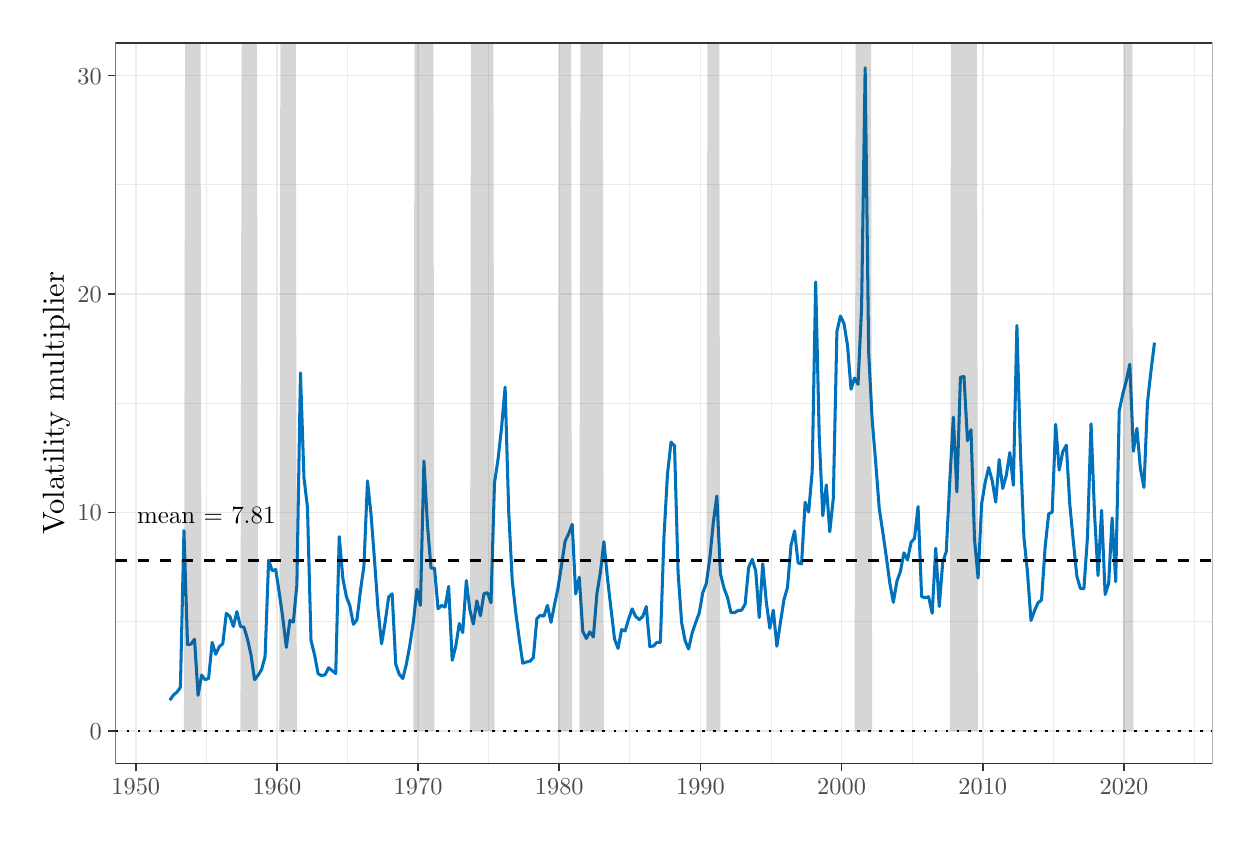
\begin{tikzpicture}[x=1pt,y=1pt]
\definecolor{fillColor}{RGB}{255,255,255}
\path[use as bounding box,fill=fillColor,fill opacity=0.00] (0,0) rectangle (433.62,289.08);
\begin{scope}
\path[clip] (  0.00,  0.00) rectangle (433.62,289.08);
\definecolor{drawColor}{RGB}{255,255,255}
\definecolor{fillColor}{RGB}{255,255,255}

\path[draw=drawColor,line width= 0.6pt,line join=round,line cap=round,fill=fillColor] (  0.00,  0.00) rectangle (433.62,289.08);
\end{scope}
\begin{scope}
\path[clip] ( 31.71, 23.11) rectangle (428.12,283.58);
\definecolor{fillColor}{RGB}{255,255,255}

\path[fill=fillColor] ( 31.71, 23.11) rectangle (428.12,283.58);
\definecolor{drawColor}{gray}{0.92}

\path[draw=drawColor,line width= 0.3pt,line join=round] ( 31.71, 74.41) --
	(428.12, 74.41);

\path[draw=drawColor,line width= 0.3pt,line join=round] ( 31.71,153.34) --
	(428.12,153.34);

\path[draw=drawColor,line width= 0.3pt,line join=round] ( 31.71,232.28) --
	(428.12,232.28);

\path[draw=drawColor,line width= 0.3pt,line join=round] ( 64.56, 23.11) --
	( 64.56,283.58);

\path[draw=drawColor,line width= 0.3pt,line join=round] (115.57, 23.11) --
	(115.57,283.58);

\path[draw=drawColor,line width= 0.3pt,line join=round] (166.59, 23.11) --
	(166.59,283.58);

\path[draw=drawColor,line width= 0.3pt,line join=round] (217.60, 23.11) --
	(217.60,283.58);

\path[draw=drawColor,line width= 0.3pt,line join=round] (268.61, 23.11) --
	(268.61,283.58);

\path[draw=drawColor,line width= 0.3pt,line join=round] (319.62, 23.11) --
	(319.62,283.58);

\path[draw=drawColor,line width= 0.3pt,line join=round] (370.64, 23.11) --
	(370.64,283.58);

\path[draw=drawColor,line width= 0.3pt,line join=round] (421.64, 23.11) --
	(421.64,283.58);

\path[draw=drawColor,line width= 0.6pt,line join=round] ( 31.71, 34.95) --
	(428.12, 34.95);

\path[draw=drawColor,line width= 0.6pt,line join=round] ( 31.71,113.88) --
	(428.12,113.88);

\path[draw=drawColor,line width= 0.6pt,line join=round] ( 31.71,192.81) --
	(428.12,192.81);

\path[draw=drawColor,line width= 0.6pt,line join=round] ( 31.71,271.74) --
	(428.12,271.74);

\path[draw=drawColor,line width= 0.6pt,line join=round] ( 39.06, 23.11) --
	( 39.06,283.58);

\path[draw=drawColor,line width= 0.6pt,line join=round] ( 90.06, 23.11) --
	( 90.06,283.58);

\path[draw=drawColor,line width= 0.6pt,line join=round] (141.08, 23.11) --
	(141.08,283.58);

\path[draw=drawColor,line width= 0.6pt,line join=round] (192.09, 23.11) --
	(192.09,283.58);

\path[draw=drawColor,line width= 0.6pt,line join=round] (243.11, 23.11) --
	(243.11,283.58);

\path[draw=drawColor,line width= 0.6pt,line join=round] (294.11, 23.11) --
	(294.11,283.58);

\path[draw=drawColor,line width= 0.6pt,line join=round] (345.13, 23.11) --
	(345.13,283.58);

\path[draw=drawColor,line width= 0.6pt,line join=round] (396.14, 23.11) --
	(396.14,283.58);
\definecolor{drawColor}{RGB}{0,114,189}

\path[draw=drawColor,line width= 1.1pt,line join=round] ( 51.38, 46.04) --
	( 52.66, 47.92) --
	( 53.93, 48.94) --
	( 55.19, 50.73) --
	( 56.47,107.36) --
	( 57.76, 66.17) --
	( 59.03, 66.34) --
	( 60.29, 68.09) --
	( 61.57, 47.82) --
	( 62.86, 55.13) --
	( 64.13, 53.47) --
	( 65.38, 53.96) --
	( 66.67, 66.96) --
	( 67.95, 62.65) --
	( 69.22, 65.38) --
	( 70.50, 66.45) --
	( 71.78, 77.44) --
	( 73.07, 76.31) --
	( 74.34, 72.68) --
	( 75.59, 78.09) --
	( 76.88, 72.69) --
	( 78.16, 72.45) --
	( 79.43, 68.14) --
	( 80.69, 62.51) --
	( 81.98, 53.49) --
	( 83.26, 55.04) --
	( 84.53, 57.15) --
	( 85.79, 61.88) --
	( 87.07, 96.65) --
	( 88.36, 92.86) --
	( 89.63, 93.25) --
	( 90.90, 84.90) --
	( 92.19, 75.80) --
	( 93.47, 65.15) --
	( 94.74, 74.90) --
	( 96.00, 74.28) --
	( 97.28, 87.82) --
	( 98.57,164.32) --
	( 99.84,126.39) --
	(101.10,115.80) --
	(102.38, 67.66) --
	(103.67, 62.44) --
	(104.94, 55.65) --
	(106.19, 54.93) --
	(107.48, 55.25) --
	(108.76, 57.79) --
	(110.03, 56.74) --
	(111.31, 55.69) --
	(112.59,105.19) --
	(113.88, 90.17) --
	(115.15, 83.51) --
	(116.40, 80.30) --
	(117.69, 73.48) --
	(118.97, 75.10) --
	(120.24, 85.61) --
	(121.50, 94.53) --
	(122.79,125.28) --
	(124.07,113.29) --
	(125.34, 96.52) --
	(126.60, 78.82) --
	(127.88, 66.42) --
	(129.17, 74.21) --
	(130.44, 83.33) --
	(131.71, 84.53) --
	(133.00, 59.04) --
	(134.28, 55.40) --
	(135.55, 53.88) --
	(136.81, 59.00) --
	(138.09, 65.88) --
	(139.38, 74.47) --
	(140.65, 86.13) --
	(141.91, 80.35) --
	(143.19,132.47) --
	(144.48,109.11) --
	(145.75, 93.79) --
	(147.00, 93.81) --
	(148.29, 79.11) --
	(149.57, 80.33) --
	(150.84, 79.69) --
	(152.12, 87.19) --
	(153.40, 60.48) --
	(154.69, 65.54) --
	(155.96, 73.79) --
	(157.21, 70.50) --
	(158.50, 89.30) --
	(159.78, 78.62) --
	(161.05, 73.57) --
	(162.31, 81.95) --
	(163.60, 76.57) --
	(164.88, 84.54) --
	(166.15, 84.92) --
	(167.41, 81.25) --
	(168.69,124.67) --
	(169.98,133.24) --
	(171.25,144.72) --
	(172.52,159.20) --
	(173.81,114.41) --
	(175.09, 89.36) --
	(176.36, 77.86) --
	(177.62, 68.31) --
	(178.90, 59.44) --
	(180.19, 59.86) --
	(181.46, 60.11) --
	(182.72, 61.41) --
	(184.00, 75.59) --
	(185.29, 76.77) --
	(186.56, 76.43) --
	(187.81, 80.34) --
	(189.10, 74.19) --
	(190.38, 80.62) --
	(191.65, 86.70) --
	(192.93, 95.02) --
	(194.21,103.55) --
	(195.50,106.24) --
	(196.77,109.62) --
	(198.02, 84.44) --
	(199.31, 90.53) --
	(200.59, 70.97) --
	(201.86, 68.37) --
	(203.12, 70.77) --
	(204.41, 68.90) --
	(205.69, 84.51) --
	(206.96, 92.28) --
	(208.22,103.34) --
	(209.50, 90.26) --
	(210.79, 79.02) --
	(212.06, 68.19) --
	(213.33, 64.78) --
	(214.62, 71.59) --
	(215.90, 71.11) --
	(217.17, 75.45) --
	(218.43, 79.06) --
	(219.71, 76.33) --
	(221.00, 75.14) --
	(222.27, 76.35) --
	(223.53, 79.89) --
	(224.81, 65.43) --
	(226.10, 65.65) --
	(227.37, 66.94) --
	(228.62, 66.92) --
	(229.91,104.88) --
	(231.19,127.79) --
	(232.47,139.32) --
	(233.74,137.96) --
	(235.02, 92.13) --
	(236.31, 74.07) --
	(237.58, 67.51) --
	(238.83, 64.58) --
	(240.12, 70.42) --
	(241.40, 74.14) --
	(242.67, 77.61) --
	(243.93, 84.85) --
	(245.22, 88.23) --
	(246.50, 97.43) --
	(247.77,110.46) --
	(249.03,119.86) --
	(250.31, 91.89) --
	(251.60, 86.58) --
	(252.87, 83.20) --
	(254.14, 77.70) --
	(255.43, 77.71) --
	(256.71, 78.46) --
	(257.98, 78.60) --
	(259.24, 80.78) --
	(260.52, 94.01) --
	(261.81, 96.94) --
	(263.08, 92.79) --
	(264.34, 75.94) --
	(265.62, 95.34) --
	(266.91, 81.41) --
	(268.18, 72.06) --
	(269.43, 78.57) --
	(270.72, 65.55) --
	(272.00, 74.10) --
	(273.28, 82.34) --
	(274.55, 86.82) --
	(275.83,102.05) --
	(277.12,107.22) --
	(278.39, 95.68) --
	(279.64, 95.33) --
	(280.93,117.59) --
	(282.21,114.06) --
	(283.48,128.77) --
	(284.74,197.19) --
	(286.03,141.29) --
	(287.31,112.71) --
	(288.58,123.87) --
	(289.84,106.92) --
	(291.12,119.08) --
	(292.41,179.23) --
	(293.68,184.88) --
	(294.95,182.22) --
	(296.24,174.31) --
	(297.52,158.42) --
	(298.79,162.48) --
	(300.05,160.19) --
	(301.33,187.92) --
	(302.62,274.60) --
	(303.89,171.71) --
	(305.15,147.57) --
	(306.43,131.95) --
	(307.72,115.27) --
	(308.99,106.81) --
	(310.24, 98.00) --
	(311.53, 88.40) --
	(312.81, 81.43) --
	(314.09, 89.07) --
	(315.36, 92.56) --
	(316.64, 99.33) --
	(317.93, 96.72) --
	(319.20,103.10) --
	(320.45,104.53) --
	(321.74,116.02) --
	(323.02, 83.51) --
	(324.29, 83.06) --
	(325.55, 83.43) --
	(326.84, 77.46) --
	(328.12,100.99) --
	(329.39, 79.90) --
	(330.65, 95.92) --
	(331.93, 99.75) --
	(333.22,125.71) --
	(334.49,148.38) --
	(335.76,121.34) --
	(337.05,162.78) --
	(338.33,163.01) --
	(339.60,139.83) --
	(340.86,143.81) --
	(342.14,104.14) --
	(343.43, 90.21) --
	(344.70,116.95) --
	(345.96,124.65) --
	(347.24,130.15) --
	(348.53,125.38) --
	(349.80,117.64) --
	(351.05,133.01) --
	(352.34,122.57) --
	(353.62,127.25) --
	(354.90,135.57) --
	(356.17,123.71) --
	(357.45,181.47) --
	(358.74,135.49) --
	(360.01,104.75) --
	(361.26, 92.42) --
	(362.55, 74.86) --
	(363.83, 78.44) --
	(365.10, 81.29) --
	(366.36, 82.26) --
	(367.65,101.35) --
	(368.93,113.41) --
	(370.20,113.98) --
	(371.46,145.74) --
	(372.74,129.18) --
	(374.03,135.87) --
	(375.30,138.21) --
	(376.57,116.84) --
	(377.86,103.29) --
	(379.14, 90.72) --
	(380.41, 86.41) --
	(381.67, 86.35) --
	(382.95,104.94) --
	(384.24,145.94) --
	(385.51,113.26) --
	(386.77, 91.11) --
	(388.05,114.68) --
	(389.34, 84.25) --
	(390.61, 88.31) --
	(391.86,111.92) --
	(393.15, 88.88) --
	(394.43,150.61) --
	(395.71,156.70) --
	(396.98,161.47) --
	(398.26,167.46) --
	(399.55,136.03) --
	(400.82,144.31) --
	(402.07,129.83) --
	(403.36,122.94) --
	(404.64,153.67) --
	(405.91,165.12) --
	(407.17,175.26);
\definecolor{fillColor}{RGB}{51,51,51}

\path[fill=fillColor,fill opacity=0.20] ( 50.09, 34.95) --
	( 50.45, 34.95) --
	( 51.02, 34.95) --
	( 51.38, 34.95) --
	( 51.73, 34.95) --
	( 52.30, 34.95) --
	( 52.66, 34.95) --
	( 53.02, 34.95) --
	( 53.57, 34.95) --
	( 53.93, 34.95) --
	( 54.29, 34.95) --
	( 54.83, 34.95) --
	( 55.19, 34.95) --
	( 55.55, 34.95) --
	( 56.11, 34.95) --
	( 56.47, 34.95) --
	( 56.83,255.88) --
	( 57.40,603.33) --
	( 57.76,824.25) --
	( 58.12,824.25) --
	( 58.67,824.25) --
	( 59.03,824.25) --
	( 59.39,824.25) --
	( 59.93,824.25) --
	( 60.29,824.25) --
	( 60.65,824.25) --
	( 61.21,824.25) --
	( 61.57,824.25) --
	( 61.93,603.33) --
	( 62.50,255.88) --
	( 62.86, 34.95) --
	( 63.22, 34.95) --
	( 63.77, 34.95) --
	( 64.13, 34.95) --
	( 64.49, 34.95) --
	( 65.02, 34.95) --
	( 65.38, 34.95) --
	( 65.74, 34.95) --
	( 66.31, 34.95) --
	( 66.67, 34.95) --
	( 67.03, 34.95) --
	( 67.59, 34.95) --
	( 67.95, 34.95) --
	( 68.31, 34.95) --
	( 68.86, 34.95) --
	( 69.22, 34.95) --
	( 69.58, 34.95) --
	( 70.14, 34.95) --
	( 70.50, 34.95) --
	( 70.86, 34.95) --
	( 71.42, 34.95) --
	( 71.78, 34.95) --
	( 72.14, 34.95) --
	( 72.71, 34.95) --
	( 73.07, 34.95) --
	( 73.42, 34.95) --
	( 73.98, 34.95) --
	( 74.34, 34.95) --
	( 74.70, 34.95) --
	( 75.23, 34.95) --
	( 75.59, 34.95) --
	( 75.95, 34.95) --
	( 76.52, 34.95) --
	( 76.88, 34.95) --
	( 77.24,255.88) --
	( 77.80,603.33) --
	( 78.16,824.25) --
	( 78.52,824.25) --
	( 79.07,824.25) --
	( 79.43,824.25) --
	( 79.79,824.25) --
	( 80.33,824.25) --
	( 80.69,824.25) --
	( 81.05,824.25) --
	( 81.62,824.25) --
	( 81.98,824.25) --
	( 82.34,603.33) --
	( 82.90,255.88) --
	( 83.26, 34.95) --
	( 83.62, 34.95) --
	( 84.17, 34.95) --
	( 84.53, 34.95) --
	( 84.89, 34.95) --
	( 85.43, 34.95) --
	( 85.79, 34.95) --
	( 86.15, 34.95) --
	( 86.71, 34.95) --
	( 87.07, 34.95) --
	( 87.43, 34.95) --
	( 88.00, 34.95) --
	( 88.36, 34.95) --
	( 88.72, 34.95) --
	( 89.27, 34.95) --
	( 89.63, 34.95) --
	( 89.99, 34.95) --
	( 90.54, 34.95) --
	( 90.90, 34.95) --
	( 91.26,255.88) --
	( 91.83,603.33) --
	( 92.19,824.25) --
	( 92.55,824.25) --
	( 93.11,824.25) --
	( 93.47,824.25) --
	( 93.83,824.25) --
	( 94.38,824.25) --
	( 94.74,824.25) --
	( 95.10,824.25) --
	( 95.64,824.25) --
	( 96.00,824.25) --
	( 96.36,603.33) --
	( 96.92,255.88) --
	( 97.28, 34.95) --
	( 97.64, 34.95) --
	( 98.21, 34.95) --
	( 98.57, 34.95) --
	( 98.93, 34.95) --
	( 99.48, 34.95) --
	( 99.84, 34.95) --
	(100.20, 34.95) --
	(100.74, 34.95) --
	(101.10, 34.95) --
	(101.46, 34.95) --
	(102.02, 34.95) --
	(102.38, 34.95) --
	(102.74, 34.95) --
	(103.31, 34.95) --
	(103.67, 34.95) --
	(104.03, 34.95) --
	(104.58, 34.95) --
	(104.94, 34.95) --
	(105.30, 34.95) --
	(105.83, 34.95) --
	(106.19, 34.95) --
	(106.55, 34.95) --
	(107.12, 34.95) --
	(107.48, 34.95) --
	(107.84, 34.95) --
	(108.40, 34.95) --
	(108.76, 34.95) --
	(109.12, 34.95) --
	(109.67, 34.95) --
	(110.03, 34.95) --
	(110.39, 34.95) --
	(110.95, 34.95) --
	(111.31, 34.95) --
	(111.67, 34.95) --
	(112.23, 34.95) --
	(112.59, 34.95) --
	(112.95, 34.95) --
	(113.52, 34.95) --
	(113.88, 34.95) --
	(114.24, 34.95) --
	(114.79, 34.95) --
	(115.15, 34.95) --
	(115.51, 34.95) --
	(116.04, 34.95) --
	(116.40, 34.95) --
	(116.76, 34.95) --
	(117.33, 34.95) --
	(117.69, 34.95) --
	(118.05, 34.95) --
	(118.61, 34.95) --
	(118.97, 34.95) --
	(119.33, 34.95) --
	(119.88, 34.95) --
	(120.24, 34.95) --
	(120.60, 34.95) --
	(121.14, 34.95) --
	(121.50, 34.95) --
	(121.86, 34.95) --
	(122.43, 34.95) --
	(122.79, 34.95) --
	(123.15, 34.95) --
	(123.71, 34.95) --
	(124.07, 34.95) --
	(124.43, 34.95) --
	(124.98, 34.95) --
	(125.34, 34.95) --
	(125.70, 34.95) --
	(126.24, 34.95) --
	(126.60, 34.95) --
	(126.96, 34.95) --
	(127.52, 34.95) --
	(127.88, 34.95) --
	(128.24, 34.95) --
	(128.81, 34.95) --
	(129.17, 34.95) --
	(129.53, 34.95) --
	(130.08, 34.95) --
	(130.44, 34.95) --
	(130.80, 34.95) --
	(131.35, 34.95) --
	(131.71, 34.95) --
	(132.07, 34.95) --
	(132.64, 34.95) --
	(133.00, 34.95) --
	(133.36, 34.95) --
	(133.92, 34.95) --
	(134.28, 34.95) --
	(134.64, 34.95) --
	(135.19, 34.95) --
	(135.55, 34.95) --
	(135.91, 34.95) --
	(136.45, 34.95) --
	(136.81, 34.95) --
	(137.17, 34.95) --
	(137.73, 34.95) --
	(138.09, 34.95) --
	(138.45, 34.95) --
	(139.02, 34.95) --
	(139.38, 34.95) --
	(139.74,258.30) --
	(140.29,600.90) --
	(140.65,824.25) --
	(141.01,824.25) --
	(141.55,824.25) --
	(141.91,824.25) --
	(142.27,824.25) --
	(142.83,824.25) --
	(143.19,824.25) --
	(143.55,824.25) --
	(144.12,824.25) --
	(144.48,824.25) --
	(144.84,824.25) --
	(145.39,824.25) --
	(145.75,824.25) --
	(146.11,598.42) --
	(146.64,260.79) --
	(147.00, 34.95) --
	(147.36, 34.95) --
	(147.93, 34.95) --
	(148.29, 34.95) --
	(148.65, 34.95) --
	(149.21, 34.95) --
	(149.57, 34.95) --
	(149.93, 34.95) --
	(150.49, 34.95) --
	(150.84, 34.95) --
	(151.20, 34.95) --
	(151.76, 34.95) --
	(152.12, 34.95) --
	(152.48, 34.95) --
	(153.04, 34.95) --
	(153.40, 34.95) --
	(153.76, 34.95) --
	(154.33, 34.95) --
	(154.69, 34.95) --
	(155.05, 34.95) --
	(155.60, 34.95) --
	(155.96, 34.95) --
	(156.32, 34.95) --
	(156.85, 34.95) --
	(157.21, 34.95) --
	(157.57, 34.95) --
	(158.14, 34.95) --
	(158.50, 34.95) --
	(158.86, 34.95) --
	(159.42, 34.95) --
	(159.78, 34.95) --
	(160.14,258.30) --
	(160.69,600.90) --
	(161.05,824.25) --
	(161.41,824.25) --
	(161.95,824.25) --
	(162.31,824.25) --
	(162.67,824.25) --
	(163.24,824.25) --
	(163.60,824.25) --
	(163.96,824.25) --
	(164.52,824.25) --
	(164.88,824.25) --
	(165.24,824.25) --
	(165.79,824.25) --
	(166.15,824.25) --
	(166.51,824.25) --
	(167.05,824.25) --
	(167.41,824.25) --
	(167.77,603.33) --
	(168.33,255.88) --
	(168.69, 34.95) --
	(169.05, 34.95) --
	(169.62, 34.95) --
	(169.98, 34.95) --
	(170.34, 34.95) --
	(170.89, 34.95) --
	(171.25, 34.95) --
	(171.61, 34.95) --
	(172.16, 34.95) --
	(172.52, 34.95) --
	(172.88, 34.95) --
	(173.45, 34.95) --
	(173.81, 34.95) --
	(174.17, 34.95) --
	(174.73, 34.95) --
	(175.09, 34.95) --
	(175.45, 34.95) --
	(176.00, 34.95) --
	(176.36, 34.95) --
	(176.72, 34.95) --
	(177.26, 34.95) --
	(177.62, 34.95) --
	(177.98, 34.95) --
	(178.54, 34.95) --
	(178.90, 34.95) --
	(179.26, 34.95) --
	(179.83, 34.95) --
	(180.19, 34.95) --
	(180.55, 34.95) --
	(181.10, 34.95) --
	(181.46, 34.95) --
	(181.82, 34.95) --
	(182.36, 34.95) --
	(182.72, 34.95) --
	(183.08, 34.95) --
	(183.64, 34.95) --
	(184.00, 34.95) --
	(184.36, 34.95) --
	(184.93, 34.95) --
	(185.29, 34.95) --
	(185.65, 34.95) --
	(186.20, 34.95) --
	(186.56, 34.95) --
	(186.92, 34.95) --
	(187.45, 34.95) --
	(187.81, 34.95) --
	(188.17, 34.95) --
	(188.74, 34.95) --
	(189.10, 34.95) --
	(189.46, 34.95) --
	(190.02, 34.95) --
	(190.38, 34.95) --
	(190.74, 34.95) --
	(191.30, 34.95) --
	(191.65, 34.95) --
	(192.01,258.30) --
	(192.57,600.90) --
	(192.93,824.25) --
	(193.29,824.25) --
	(193.85,824.25) --
	(194.21,824.25) --
	(194.57,824.25) --
	(195.14,824.25) --
	(195.50,824.25) --
	(195.86,600.90) --
	(196.41,258.30) --
	(196.77, 34.95) --
	(197.13, 34.95) --
	(197.66, 34.95) --
	(198.02, 34.95) --
	(198.38, 34.95) --
	(198.95, 34.95) --
	(199.31, 34.95) --
	(199.67,255.88) --
	(200.23,603.33) --
	(200.59,824.25) --
	(200.95,824.25) --
	(201.50,824.25) --
	(201.86,824.25) --
	(202.22,824.25) --
	(202.76,824.25) --
	(203.12,824.25) --
	(203.48,824.25) --
	(204.05,824.25) --
	(204.41,824.25) --
	(204.77,824.25) --
	(205.33,824.25) --
	(205.69,824.25) --
	(206.05,824.25) --
	(206.60,824.25) --
	(206.96,824.25) --
	(207.32,598.42) --
	(207.86,260.79) --
	(208.22, 34.95) --
	(208.58, 34.95) --
	(209.14, 34.95) --
	(209.50, 34.95) --
	(209.86, 34.95) --
	(210.43, 34.95) --
	(210.79, 34.95) --
	(211.15, 34.95) --
	(211.70, 34.95) --
	(212.06, 34.95) --
	(212.42, 34.95) --
	(212.97, 34.95) --
	(213.33, 34.95) --
	(213.69, 34.95) --
	(214.26, 34.95) --
	(214.62, 34.95) --
	(214.98, 34.95) --
	(215.54, 34.95) --
	(215.90, 34.95) --
	(216.26, 34.95) --
	(216.81, 34.95) --
	(217.17, 34.95) --
	(217.53, 34.95) --
	(218.07, 34.95) --
	(218.43, 34.95) --
	(218.79, 34.95) --
	(219.35, 34.95) --
	(219.71, 34.95) --
	(220.07, 34.95) --
	(220.64, 34.95) --
	(221.00, 34.95) --
	(221.36, 34.95) --
	(221.91, 34.95) --
	(222.27, 34.95) --
	(222.63, 34.95) --
	(223.17, 34.95) --
	(223.53, 34.95) --
	(223.89, 34.95) --
	(224.45, 34.95) --
	(224.81, 34.95) --
	(225.17, 34.95) --
	(225.74, 34.95) --
	(226.10, 34.95) --
	(226.46, 34.95) --
	(227.01, 34.95) --
	(227.37, 34.95) --
	(227.73, 34.95) --
	(228.26, 34.95) --
	(228.62, 34.95) --
	(228.98, 34.95) --
	(229.55, 34.95) --
	(229.91, 34.95) --
	(230.27, 34.95) --
	(230.83, 34.95) --
	(231.19, 34.95) --
	(231.55, 34.95) --
	(232.11, 34.95) --
	(232.47, 34.95) --
	(232.82, 34.95) --
	(233.38, 34.95) --
	(233.74, 34.95) --
	(234.10, 34.95) --
	(234.66, 34.95) --
	(235.02, 34.95) --
	(235.38, 34.95) --
	(235.95, 34.95) --
	(236.31, 34.95) --
	(236.67, 34.95) --
	(237.22, 34.95) --
	(237.58, 34.95) --
	(237.94, 34.95) --
	(238.47, 34.95) --
	(238.83, 34.95) --
	(239.19, 34.95) --
	(239.76, 34.95) --
	(240.12, 34.95) --
	(240.48, 34.95) --
	(241.04, 34.95) --
	(241.40, 34.95) --
	(241.76, 34.95) --
	(242.31, 34.95) --
	(242.67, 34.95) --
	(243.03, 34.95) --
	(243.57, 34.95) --
	(243.93, 34.95) --
	(244.29, 34.95) --
	(244.86, 34.95) --
	(245.22, 34.95) --
	(245.58,255.88) --
	(246.14,603.33) --
	(246.50,824.25) --
	(246.86,824.25) --
	(247.41,824.25) --
	(247.77,824.25) --
	(248.13,824.25) --
	(248.67,824.25) --
	(249.03,824.25) --
	(249.39,603.33) --
	(249.95,255.88) --
	(250.31, 34.95) --
	(250.67, 34.95) --
	(251.24, 34.95) --
	(251.60, 34.95) --
	(251.96, 34.95) --
	(252.51, 34.95) --
	(252.87, 34.95) --
	(253.23, 34.95) --
	(253.78, 34.95) --
	(254.14, 34.95) --
	(254.50, 34.95) --
	(255.07, 34.95) --
	(255.43, 34.95) --
	(255.79, 34.95) --
	(256.35, 34.95) --
	(256.71, 34.95) --
	(257.07, 34.95) --
	(257.62, 34.95) --
	(257.98, 34.95) --
	(258.34, 34.95) --
	(258.88, 34.95) --
	(259.24, 34.95) --
	(259.60, 34.95) --
	(260.16, 34.95) --
	(260.52, 34.95) --
	(260.88, 34.95) --
	(261.45, 34.95) --
	(261.81, 34.95) --
	(262.17, 34.95) --
	(262.72, 34.95) --
	(263.08, 34.95) --
	(263.44, 34.95) --
	(263.98, 34.95) --
	(264.34, 34.95) --
	(264.70, 34.95) --
	(265.26, 34.95) --
	(265.62, 34.95) --
	(265.98, 34.95) --
	(266.55, 34.95) --
	(266.91, 34.95) --
	(267.27, 34.95) --
	(267.82, 34.95) --
	(268.18, 34.95) --
	(268.54, 34.95) --
	(269.07, 34.95) --
	(269.43, 34.95) --
	(269.79, 34.95) --
	(270.36, 34.95) --
	(270.72, 34.95) --
	(271.08, 34.95) --
	(271.64, 34.95) --
	(272.00, 34.95) --
	(272.36, 34.95) --
	(272.92, 34.95) --
	(273.28, 34.95) --
	(273.63, 34.95) --
	(274.19, 34.95) --
	(274.55, 34.95) --
	(274.91, 34.95) --
	(275.47, 34.95) --
	(275.83, 34.95) --
	(276.19, 34.95) --
	(276.76, 34.95) --
	(277.12, 34.95) --
	(277.48, 34.95) --
	(278.03, 34.95) --
	(278.39, 34.95) --
	(278.75, 34.95) --
	(279.28, 34.95) --
	(279.64, 34.95) --
	(280.00, 34.95) --
	(280.57, 34.95) --
	(280.93, 34.95) --
	(281.29, 34.95) --
	(281.85, 34.95) --
	(282.21, 34.95) --
	(282.57, 34.95) --
	(283.12, 34.95) --
	(283.48, 34.95) --
	(283.84, 34.95) --
	(284.38, 34.95) --
	(284.74, 34.95) --
	(285.10, 34.95) --
	(285.67, 34.95) --
	(286.03, 34.95) --
	(286.39, 34.95) --
	(286.95, 34.95) --
	(287.31, 34.95) --
	(287.67, 34.95) --
	(288.22, 34.95) --
	(288.58, 34.95) --
	(288.94, 34.95) --
	(289.48, 34.95) --
	(289.84, 34.95) --
	(290.20, 34.95) --
	(290.76, 34.95) --
	(291.12, 34.95) --
	(291.48, 34.95) --
	(292.05, 34.95) --
	(292.41, 34.95) --
	(292.77, 34.95) --
	(293.32, 34.95) --
	(293.68, 34.95) --
	(294.04, 34.95) --
	(294.59, 34.95) --
	(294.95, 34.95) --
	(295.31, 34.95) --
	(295.88, 34.95) --
	(296.24, 34.95) --
	(296.60, 34.95) --
	(297.16, 34.95) --
	(297.52, 34.95) --
	(297.88, 34.95) --
	(298.43, 34.95) --
	(298.79, 34.95) --
	(299.15,260.79) --
	(299.69,598.42) --
	(300.05,824.25) --
	(300.41,824.25) --
	(300.97,824.25) --
	(301.33,824.25) --
	(301.69,824.25) --
	(302.26,824.25) --
	(302.62,824.25) --
	(302.98,824.25) --
	(303.53,824.25) --
	(303.89,824.25) --
	(304.25,598.42) --
	(304.79,260.79) --
	(305.15, 34.95) --
	(305.51, 34.95) --
	(306.07, 34.95) --
	(306.43, 34.95) --
	(306.79, 34.95) --
	(307.36, 34.95) --
	(307.72, 34.95) --
	(308.08, 34.95) --
	(308.63, 34.95) --
	(308.99, 34.95) --
	(309.35, 34.95) --
	(309.88, 34.95) --
	(310.24, 34.95) --
	(310.60, 34.95) --
	(311.17, 34.95) --
	(311.53, 34.95) --
	(311.89, 34.95) --
	(312.45, 34.95) --
	(312.81, 34.95) --
	(313.17, 34.95) --
	(313.73, 34.95) --
	(314.09, 34.95) --
	(314.44, 34.95) --
	(315.00, 34.95) --
	(315.36, 34.95) --
	(315.72, 34.95) --
	(316.28, 34.95) --
	(316.64, 34.95) --
	(317.00, 34.95) --
	(317.57, 34.95) --
	(317.93, 34.95) --
	(318.29, 34.95) --
	(318.84, 34.95) --
	(319.20, 34.95) --
	(319.56, 34.95) --
	(320.09, 34.95) --
	(320.45, 34.95) --
	(320.81, 34.95) --
	(321.38, 34.95) --
	(321.74, 34.95) --
	(322.10, 34.95) --
	(322.66, 34.95) --
	(323.02, 34.95) --
	(323.38, 34.95) --
	(323.94, 34.95) --
	(324.29, 34.95) --
	(324.65, 34.95) --
	(325.19, 34.95) --
	(325.55, 34.95) --
	(325.91, 34.95) --
	(326.48, 34.95) --
	(326.84, 34.95) --
	(327.20, 34.95) --
	(327.76, 34.95) --
	(328.12, 34.95) --
	(328.48, 34.95) --
	(329.03, 34.95) --
	(329.39, 34.95) --
	(329.75, 34.95) --
	(330.29, 34.95) --
	(330.65, 34.95) --
	(331.01, 34.95) --
	(331.57, 34.95) --
	(331.93, 34.95) --
	(332.29, 34.95) --
	(332.86, 34.95) --
	(333.22, 34.95) --
	(333.58,258.30) --
	(334.13,600.90) --
	(334.49,824.25) --
	(334.85,824.25) --
	(335.40,824.25) --
	(335.76,824.25) --
	(336.12,824.25) --
	(336.69,824.25) --
	(337.05,824.25) --
	(337.41,824.25) --
	(337.97,824.25) --
	(338.33,824.25) --
	(338.69,824.25) --
	(339.24,824.25) --
	(339.60,824.25) --
	(339.96,824.25) --
	(340.50,824.25) --
	(340.86,824.25) --
	(341.22,824.25) --
	(341.78,824.25) --
	(342.14,824.25) --
	(342.50,603.33) --
	(343.07,255.88) --
	(343.43, 34.95) --
	(343.79, 34.95) --
	(344.34, 34.95) --
	(344.70, 34.95) --
	(345.06, 34.95) --
	(345.60, 34.95) --
	(345.96, 34.95) --
	(346.32, 34.95) --
	(346.88, 34.95) --
	(347.24, 34.95) --
	(347.60, 34.95) --
	(348.17, 34.95) --
	(348.53, 34.95) --
	(348.89, 34.95) --
	(349.44, 34.95) --
	(349.80, 34.95) --
	(350.16, 34.95) --
	(350.69, 34.95) --
	(351.05, 34.95) --
	(351.41, 34.95) --
	(351.98, 34.95) --
	(352.34, 34.95) --
	(352.70, 34.95) --
	(353.26, 34.95) --
	(353.62, 34.95) --
	(353.98, 34.95) --
	(354.54, 34.95) --
	(354.90, 34.95) --
	(355.26, 34.95) --
	(355.81, 34.95) --
	(356.17, 34.95) --
	(356.53, 34.95) --
	(357.09, 34.95) --
	(357.45, 34.95) --
	(357.81, 34.95) --
	(358.38, 34.95) --
	(358.74, 34.95) --
	(359.10, 34.95) --
	(359.65, 34.95) --
	(360.01, 34.95) --
	(360.37, 34.95) --
	(360.90, 34.95) --
	(361.26, 34.95) --
	(361.62, 34.95) --
	(362.19, 34.95) --
	(362.55, 34.95) --
	(362.91, 34.95) --
	(363.47, 34.95) --
	(363.83, 34.95) --
	(364.19, 34.95) --
	(364.75, 34.95) --
	(365.10, 34.95) --
	(365.46, 34.95) --
	(366.00, 34.95) --
	(366.36, 34.95) --
	(366.72, 34.95) --
	(367.29, 34.95) --
	(367.65, 34.95) --
	(368.01, 34.95) --
	(368.57, 34.95) --
	(368.93, 34.95) --
	(369.29, 34.95) --
	(369.84, 34.95) --
	(370.20, 34.95) --
	(370.56, 34.95) --
	(371.10, 34.95) --
	(371.46, 34.95) --
	(371.82, 34.95) --
	(372.38, 34.95) --
	(372.74, 34.95) --
	(373.10, 34.95) --
	(373.67, 34.95) --
	(374.03, 34.95) --
	(374.39, 34.95) --
	(374.94, 34.95) --
	(375.30, 34.95) --
	(375.66, 34.95) --
	(376.21, 34.95) --
	(376.57, 34.95) --
	(376.93, 34.95) --
	(377.50, 34.95) --
	(377.86, 34.95) --
	(378.22, 34.95) --
	(378.78, 34.95) --
	(379.14, 34.95) --
	(379.50, 34.95) --
	(380.05, 34.95) --
	(380.41, 34.95) --
	(380.77, 34.95) --
	(381.31, 34.95) --
	(381.67, 34.95) --
	(382.03, 34.95) --
	(382.59, 34.95) --
	(382.95, 34.95) --
	(383.31, 34.95) --
	(383.88, 34.95) --
	(384.24, 34.95) --
	(384.60, 34.95) --
	(385.15, 34.95) --
	(385.51, 34.95) --
	(385.87, 34.95) --
	(386.41, 34.95) --
	(386.77, 34.95) --
	(387.13, 34.95) --
	(387.69, 34.95) --
	(388.05, 34.95) --
	(388.41, 34.95) --
	(388.98, 34.95) --
	(389.34, 34.95) --
	(389.70, 34.95) --
	(390.25, 34.95) --
	(390.61, 34.95) --
	(390.97, 34.95) --
	(391.51, 34.95) --
	(391.86, 34.95) --
	(392.22, 34.95) --
	(392.79, 34.95) --
	(393.15, 34.95) --
	(393.51, 34.95) --
	(394.07, 34.95) --
	(394.43, 34.95) --
	(394.79, 34.95) --
	(395.35, 34.95) --
	(395.71, 34.95) --
	(396.07,258.30) --
	(396.62,600.90) --
	(396.98,824.25) --
	(397.34,824.25) --
	(397.90,824.25) --
	(398.26,824.25) --
	(398.62,603.33) --
	(399.19,255.88) --
	(399.55, 34.95) --
	(399.91, 34.95) --
	(400.46, 34.95) --
	(400.82, 34.95) --
	(401.18, 34.95) --
	(401.71, 34.95) --
	(402.07, 34.95) --
	(402.43, 34.95) --
	(403.00, 34.95) --
	(403.36, 34.95) --
	(403.72, 34.95) --
	(404.28, 34.95) --
	(404.64, 34.95) --
	(405.00, 34.95) --
	(405.56, 34.95) --
	(405.91, 34.95) --
	(406.27, 34.95) --
	(406.81, 34.95) --
	(407.17, 34.95) --
	(407.53, 34.95) --
	(408.10, 34.95) --
	(408.46, 34.95) --
	(408.82, 34.95) --
	(409.38, 34.95) --
	(409.74, 34.95) --
	(410.10, 34.95) --
	(409.74, 34.95) --
	(409.38, 34.95) --
	(408.82, 34.95) --
	(408.46, 34.95) --
	(408.10, 34.95) --
	(407.53, 34.95) --
	(407.17, 34.95) --
	(406.81, 34.95) --
	(406.27, 34.95) --
	(405.91, 34.95) --
	(405.56, 34.95) --
	(405.00, 34.95) --
	(404.64, 34.95) --
	(404.28, 34.95) --
	(403.72, 34.95) --
	(403.36, 34.95) --
	(403.00, 34.95) --
	(402.43, 34.95) --
	(402.07, 34.95) --
	(401.71, 34.95) --
	(401.18, 34.95) --
	(400.82, 34.95) --
	(400.46, 34.95) --
	(399.91, 34.95) --
	(399.55, 34.95) --
	(399.19, 34.95) --
	(398.62, 34.95) --
	(398.26, 34.95) --
	(397.90, 34.95) --
	(397.34, 34.95) --
	(396.98, 34.95) --
	(396.62, 34.95) --
	(396.07, 34.95) --
	(395.71, 34.95) --
	(395.35, 34.95) --
	(394.79, 34.95) --
	(394.43, 34.95) --
	(394.07, 34.95) --
	(393.51, 34.95) --
	(393.15, 34.95) --
	(392.79, 34.95) --
	(392.22, 34.95) --
	(391.86, 34.95) --
	(391.51, 34.95) --
	(390.97, 34.95) --
	(390.61, 34.95) --
	(390.25, 34.95) --
	(389.70, 34.95) --
	(389.34, 34.95) --
	(388.98, 34.95) --
	(388.41, 34.95) --
	(388.05, 34.95) --
	(387.69, 34.95) --
	(387.13, 34.95) --
	(386.77, 34.95) --
	(386.41, 34.95) --
	(385.87, 34.95) --
	(385.51, 34.95) --
	(385.15, 34.95) --
	(384.60, 34.95) --
	(384.24, 34.95) --
	(383.88, 34.95) --
	(383.31, 34.95) --
	(382.95, 34.95) --
	(382.59, 34.95) --
	(382.03, 34.95) --
	(381.67, 34.95) --
	(381.31, 34.95) --
	(380.77, 34.95) --
	(380.41, 34.95) --
	(380.05, 34.95) --
	(379.50, 34.95) --
	(379.14, 34.95) --
	(378.78, 34.95) --
	(378.22, 34.95) --
	(377.86, 34.95) --
	(377.50, 34.95) --
	(376.93, 34.95) --
	(376.57, 34.95) --
	(376.21, 34.95) --
	(375.66, 34.95) --
	(375.30, 34.95) --
	(374.94, 34.95) --
	(374.39, 34.95) --
	(374.03, 34.95) --
	(373.67, 34.95) --
	(373.10, 34.95) --
	(372.74, 34.95) --
	(372.38, 34.95) --
	(371.82, 34.95) --
	(371.46, 34.95) --
	(371.10, 34.95) --
	(370.56, 34.95) --
	(370.20, 34.95) --
	(369.84, 34.95) --
	(369.29, 34.95) --
	(368.93, 34.95) --
	(368.57, 34.95) --
	(368.01, 34.95) --
	(367.65, 34.95) --
	(367.29, 34.95) --
	(366.72, 34.95) --
	(366.36, 34.95) --
	(366.00, 34.95) --
	(365.46, 34.95) --
	(365.10, 34.95) --
	(364.75, 34.95) --
	(364.19, 34.95) --
	(363.83, 34.95) --
	(363.47, 34.95) --
	(362.91, 34.95) --
	(362.55, 34.95) --
	(362.19, 34.95) --
	(361.62, 34.95) --
	(361.26, 34.95) --
	(360.90, 34.95) --
	(360.37, 34.95) --
	(360.01, 34.95) --
	(359.65, 34.95) --
	(359.10, 34.95) --
	(358.74, 34.95) --
	(358.38, 34.95) --
	(357.81, 34.95) --
	(357.45, 34.95) --
	(357.09, 34.95) --
	(356.53, 34.95) --
	(356.17, 34.95) --
	(355.81, 34.95) --
	(355.26, 34.95) --
	(354.90, 34.95) --
	(354.54, 34.95) --
	(353.98, 34.95) --
	(353.62, 34.95) --
	(353.26, 34.95) --
	(352.70, 34.95) --
	(352.34, 34.95) --
	(351.98, 34.95) --
	(351.41, 34.95) --
	(351.05, 34.95) --
	(350.69, 34.95) --
	(350.16, 34.95) --
	(349.80, 34.95) --
	(349.44, 34.95) --
	(348.89, 34.95) --
	(348.53, 34.95) --
	(348.17, 34.95) --
	(347.60, 34.95) --
	(347.24, 34.95) --
	(346.88, 34.95) --
	(346.32, 34.95) --
	(345.96, 34.95) --
	(345.60, 34.95) --
	(345.06, 34.95) --
	(344.70, 34.95) --
	(344.34, 34.95) --
	(343.79, 34.95) --
	(343.43, 34.95) --
	(343.07, 34.95) --
	(342.50, 34.95) --
	(342.14, 34.95) --
	(341.78, 34.95) --
	(341.22, 34.95) --
	(340.86, 34.95) --
	(340.50, 34.95) --
	(339.96, 34.95) --
	(339.60, 34.95) --
	(339.24, 34.95) --
	(338.69, 34.95) --
	(338.33, 34.95) --
	(337.97, 34.95) --
	(337.41, 34.95) --
	(337.05, 34.95) --
	(336.69, 34.95) --
	(336.12, 34.95) --
	(335.76, 34.95) --
	(335.40, 34.95) --
	(334.85, 34.95) --
	(334.49, 34.95) --
	(334.13, 34.95) --
	(333.58, 34.95) --
	(333.22, 34.95) --
	(332.86, 34.95) --
	(332.29, 34.95) --
	(331.93, 34.95) --
	(331.57, 34.95) --
	(331.01, 34.95) --
	(330.65, 34.95) --
	(330.29, 34.95) --
	(329.75, 34.95) --
	(329.39, 34.95) --
	(329.03, 34.95) --
	(328.48, 34.95) --
	(328.12, 34.95) --
	(327.76, 34.95) --
	(327.20, 34.95) --
	(326.84, 34.95) --
	(326.48, 34.95) --
	(325.91, 34.95) --
	(325.55, 34.95) --
	(325.19, 34.95) --
	(324.65, 34.95) --
	(324.29, 34.95) --
	(323.94, 34.95) --
	(323.38, 34.95) --
	(323.02, 34.95) --
	(322.66, 34.95) --
	(322.10, 34.95) --
	(321.74, 34.95) --
	(321.38, 34.95) --
	(320.81, 34.95) --
	(320.45, 34.95) --
	(320.09, 34.95) --
	(319.56, 34.95) --
	(319.20, 34.95) --
	(318.84, 34.95) --
	(318.29, 34.95) --
	(317.93, 34.95) --
	(317.57, 34.95) --
	(317.00, 34.95) --
	(316.64, 34.95) --
	(316.28, 34.95) --
	(315.72, 34.95) --
	(315.36, 34.95) --
	(315.00, 34.95) --
	(314.44, 34.95) --
	(314.09, 34.95) --
	(313.73, 34.95) --
	(313.17, 34.95) --
	(312.81, 34.95) --
	(312.45, 34.95) --
	(311.89, 34.95) --
	(311.53, 34.95) --
	(311.17, 34.95) --
	(310.60, 34.95) --
	(310.24, 34.95) --
	(309.88, 34.95) --
	(309.35, 34.95) --
	(308.99, 34.95) --
	(308.63, 34.95) --
	(308.08, 34.95) --
	(307.72, 34.95) --
	(307.36, 34.95) --
	(306.79, 34.95) --
	(306.43, 34.95) --
	(306.07, 34.95) --
	(305.51, 34.95) --
	(305.15, 34.95) --
	(304.79, 34.95) --
	(304.25, 34.95) --
	(303.89, 34.95) --
	(303.53, 34.95) --
	(302.98, 34.95) --
	(302.62, 34.95) --
	(302.26, 34.95) --
	(301.69, 34.95) --
	(301.33, 34.95) --
	(300.97, 34.95) --
	(300.41, 34.95) --
	(300.05, 34.95) --
	(299.69, 34.95) --
	(299.15, 34.95) --
	(298.79, 34.95) --
	(298.43, 34.95) --
	(297.88, 34.95) --
	(297.52, 34.95) --
	(297.16, 34.95) --
	(296.60, 34.95) --
	(296.24, 34.95) --
	(295.88, 34.95) --
	(295.31, 34.95) --
	(294.95, 34.95) --
	(294.59, 34.95) --
	(294.04, 34.95) --
	(293.68, 34.95) --
	(293.32, 34.95) --
	(292.77, 34.95) --
	(292.41, 34.95) --
	(292.05, 34.95) --
	(291.48, 34.95) --
	(291.12, 34.95) --
	(290.76, 34.95) --
	(290.20, 34.95) --
	(289.84, 34.95) --
	(289.48, 34.95) --
	(288.94, 34.95) --
	(288.58, 34.95) --
	(288.22, 34.95) --
	(287.67, 34.95) --
	(287.31, 34.95) --
	(286.95, 34.95) --
	(286.39, 34.95) --
	(286.03, 34.95) --
	(285.67, 34.95) --
	(285.10, 34.95) --
	(284.74, 34.95) --
	(284.38, 34.95) --
	(283.84, 34.95) --
	(283.48, 34.95) --
	(283.12, 34.95) --
	(282.57, 34.95) --
	(282.21, 34.95) --
	(281.85, 34.95) --
	(281.29, 34.95) --
	(280.93, 34.95) --
	(280.57, 34.95) --
	(280.00, 34.95) --
	(279.64, 34.95) --
	(279.28, 34.95) --
	(278.75, 34.95) --
	(278.39, 34.95) --
	(278.03, 34.95) --
	(277.48, 34.95) --
	(277.12, 34.95) --
	(276.76, 34.95) --
	(276.19, 34.95) --
	(275.83, 34.95) --
	(275.47, 34.95) --
	(274.91, 34.95) --
	(274.55, 34.95) --
	(274.19, 34.95) --
	(273.63, 34.95) --
	(273.28, 34.95) --
	(272.92, 34.95) --
	(272.36, 34.95) --
	(272.00, 34.95) --
	(271.64, 34.95) --
	(271.08, 34.95) --
	(270.72, 34.95) --
	(270.36, 34.95) --
	(269.79, 34.95) --
	(269.43, 34.95) --
	(269.07, 34.95) --
	(268.54, 34.95) --
	(268.18, 34.95) --
	(267.82, 34.95) --
	(267.27, 34.95) --
	(266.91, 34.95) --
	(266.55, 34.95) --
	(265.98, 34.95) --
	(265.62, 34.95) --
	(265.26, 34.95) --
	(264.70, 34.95) --
	(264.34, 34.95) --
	(263.98, 34.95) --
	(263.44, 34.95) --
	(263.08, 34.95) --
	(262.72, 34.95) --
	(262.17, 34.95) --
	(261.81, 34.95) --
	(261.45, 34.95) --
	(260.88, 34.95) --
	(260.52, 34.95) --
	(260.16, 34.95) --
	(259.60, 34.95) --
	(259.24, 34.95) --
	(258.88, 34.95) --
	(258.34, 34.95) --
	(257.98, 34.95) --
	(257.62, 34.95) --
	(257.07, 34.95) --
	(256.71, 34.95) --
	(256.35, 34.95) --
	(255.79, 34.95) --
	(255.43, 34.95) --
	(255.07, 34.95) --
	(254.50, 34.95) --
	(254.14, 34.95) --
	(253.78, 34.95) --
	(253.23, 34.95) --
	(252.87, 34.95) --
	(252.51, 34.95) --
	(251.96, 34.95) --
	(251.60, 34.95) --
	(251.24, 34.95) --
	(250.67, 34.95) --
	(250.31, 34.95) --
	(249.95, 34.95) --
	(249.39, 34.95) --
	(249.03, 34.95) --
	(248.67, 34.95) --
	(248.13, 34.95) --
	(247.77, 34.95) --
	(247.41, 34.95) --
	(246.86, 34.95) --
	(246.50, 34.95) --
	(246.14, 34.95) --
	(245.58, 34.95) --
	(245.22, 34.95) --
	(244.86, 34.95) --
	(244.29, 34.95) --
	(243.93, 34.95) --
	(243.57, 34.95) --
	(243.03, 34.95) --
	(242.67, 34.95) --
	(242.31, 34.95) --
	(241.76, 34.95) --
	(241.40, 34.95) --
	(241.04, 34.95) --
	(240.48, 34.95) --
	(240.12, 34.95) --
	(239.76, 34.95) --
	(239.19, 34.95) --
	(238.83, 34.95) --
	(238.47, 34.95) --
	(237.94, 34.95) --
	(237.58, 34.95) --
	(237.22, 34.95) --
	(236.67, 34.95) --
	(236.31, 34.95) --
	(235.95, 34.95) --
	(235.38, 34.95) --
	(235.02, 34.95) --
	(234.66, 34.95) --
	(234.10, 34.95) --
	(233.74, 34.95) --
	(233.38, 34.95) --
	(232.82, 34.95) --
	(232.47, 34.95) --
	(232.11, 34.95) --
	(231.55, 34.95) --
	(231.19, 34.95) --
	(230.83, 34.95) --
	(230.27, 34.95) --
	(229.91, 34.95) --
	(229.55, 34.95) --
	(228.98, 34.95) --
	(228.62, 34.95) --
	(228.26, 34.95) --
	(227.73, 34.95) --
	(227.37, 34.95) --
	(227.01, 34.95) --
	(226.46, 34.95) --
	(226.10, 34.95) --
	(225.74, 34.95) --
	(225.17, 34.95) --
	(224.81, 34.95) --
	(224.45, 34.95) --
	(223.89, 34.95) --
	(223.53, 34.95) --
	(223.17, 34.95) --
	(222.63, 34.95) --
	(222.27, 34.95) --
	(221.91, 34.95) --
	(221.36, 34.95) --
	(221.00, 34.95) --
	(220.64, 34.95) --
	(220.07, 34.95) --
	(219.71, 34.95) --
	(219.35, 34.95) --
	(218.79, 34.95) --
	(218.43, 34.95) --
	(218.07, 34.95) --
	(217.53, 34.95) --
	(217.17, 34.95) --
	(216.81, 34.95) --
	(216.26, 34.95) --
	(215.90, 34.95) --
	(215.54, 34.95) --
	(214.98, 34.95) --
	(214.62, 34.95) --
	(214.26, 34.95) --
	(213.69, 34.95) --
	(213.33, 34.95) --
	(212.97, 34.95) --
	(212.42, 34.95) --
	(212.06, 34.95) --
	(211.70, 34.95) --
	(211.15, 34.95) --
	(210.79, 34.95) --
	(210.43, 34.95) --
	(209.86, 34.95) --
	(209.50, 34.95) --
	(209.14, 34.95) --
	(208.58, 34.95) --
	(208.22, 34.95) --
	(207.86, 34.95) --
	(207.32, 34.95) --
	(206.96, 34.95) --
	(206.60, 34.95) --
	(206.05, 34.95) --
	(205.69, 34.95) --
	(205.33, 34.95) --
	(204.77, 34.95) --
	(204.41, 34.95) --
	(204.05, 34.95) --
	(203.48, 34.95) --
	(203.12, 34.95) --
	(202.76, 34.95) --
	(202.22, 34.95) --
	(201.86, 34.95) --
	(201.50, 34.95) --
	(200.95, 34.95) --
	(200.59, 34.95) --
	(200.23, 34.95) --
	(199.67, 34.95) --
	(199.31, 34.95) --
	(198.95, 34.95) --
	(198.38, 34.95) --
	(198.02, 34.95) --
	(197.66, 34.95) --
	(197.13, 34.95) --
	(196.77, 34.95) --
	(196.41, 34.95) --
	(195.86, 34.95) --
	(195.50, 34.95) --
	(195.14, 34.95) --
	(194.57, 34.95) --
	(194.21, 34.95) --
	(193.85, 34.95) --
	(193.29, 34.95) --
	(192.93, 34.95) --
	(192.57, 34.95) --
	(192.01, 34.95) --
	(191.65, 34.95) --
	(191.30, 34.95) --
	(190.74, 34.95) --
	(190.38, 34.95) --
	(190.02, 34.95) --
	(189.46, 34.95) --
	(189.10, 34.95) --
	(188.74, 34.95) --
	(188.17, 34.95) --
	(187.81, 34.95) --
	(187.45, 34.95) --
	(186.92, 34.95) --
	(186.56, 34.95) --
	(186.20, 34.95) --
	(185.65, 34.95) --
	(185.29, 34.95) --
	(184.93, 34.95) --
	(184.36, 34.95) --
	(184.00, 34.95) --
	(183.64, 34.95) --
	(183.08, 34.95) --
	(182.72, 34.95) --
	(182.36, 34.95) --
	(181.82, 34.95) --
	(181.46, 34.95) --
	(181.10, 34.95) --
	(180.55, 34.95) --
	(180.19, 34.95) --
	(179.83, 34.95) --
	(179.26, 34.95) --
	(178.90, 34.95) --
	(178.54, 34.95) --
	(177.98, 34.95) --
	(177.62, 34.95) --
	(177.26, 34.95) --
	(176.72, 34.95) --
	(176.36, 34.95) --
	(176.00, 34.95) --
	(175.45, 34.95) --
	(175.09, 34.95) --
	(174.73, 34.95) --
	(174.17, 34.95) --
	(173.81, 34.95) --
	(173.45, 34.95) --
	(172.88, 34.95) --
	(172.52, 34.95) --
	(172.16, 34.95) --
	(171.61, 34.95) --
	(171.25, 34.95) --
	(170.89, 34.95) --
	(170.34, 34.95) --
	(169.98, 34.95) --
	(169.62, 34.95) --
	(169.05, 34.95) --
	(168.69, 34.95) --
	(168.33, 34.95) --
	(167.77, 34.95) --
	(167.41, 34.95) --
	(167.05, 34.95) --
	(166.51, 34.95) --
	(166.15, 34.95) --
	(165.79, 34.95) --
	(165.24, 34.95) --
	(164.88, 34.95) --
	(164.52, 34.95) --
	(163.96, 34.95) --
	(163.60, 34.95) --
	(163.24, 34.95) --
	(162.67, 34.95) --
	(162.31, 34.95) --
	(161.95, 34.95) --
	(161.41, 34.95) --
	(161.05, 34.95) --
	(160.69, 34.95) --
	(160.14, 34.95) --
	(159.78, 34.95) --
	(159.42, 34.95) --
	(158.86, 34.95) --
	(158.50, 34.95) --
	(158.14, 34.95) --
	(157.57, 34.95) --
	(157.21, 34.95) --
	(156.85, 34.95) --
	(156.32, 34.95) --
	(155.96, 34.95) --
	(155.60, 34.95) --
	(155.05, 34.95) --
	(154.69, 34.95) --
	(154.33, 34.95) --
	(153.76, 34.95) --
	(153.40, 34.95) --
	(153.04, 34.95) --
	(152.48, 34.95) --
	(152.12, 34.95) --
	(151.76, 34.95) --
	(151.20, 34.95) --
	(150.84, 34.95) --
	(150.49, 34.95) --
	(149.93, 34.95) --
	(149.57, 34.95) --
	(149.21, 34.95) --
	(148.65, 34.95) --
	(148.29, 34.95) --
	(147.93, 34.95) --
	(147.36, 34.95) --
	(147.00, 34.95) --
	(146.64, 34.95) --
	(146.11, 34.95) --
	(145.75, 34.95) --
	(145.39, 34.95) --
	(144.84, 34.95) --
	(144.48, 34.95) --
	(144.12, 34.95) --
	(143.55, 34.95) --
	(143.19, 34.95) --
	(142.83, 34.95) --
	(142.27, 34.95) --
	(141.91, 34.95) --
	(141.55, 34.95) --
	(141.01, 34.95) --
	(140.65, 34.95) --
	(140.29, 34.95) --
	(139.74, 34.95) --
	(139.38, 34.95) --
	(139.02, 34.95) --
	(138.45, 34.95) --
	(138.09, 34.95) --
	(137.73, 34.95) --
	(137.17, 34.95) --
	(136.81, 34.95) --
	(136.45, 34.95) --
	(135.91, 34.95) --
	(135.55, 34.95) --
	(135.19, 34.95) --
	(134.64, 34.95) --
	(134.28, 34.95) --
	(133.92, 34.95) --
	(133.36, 34.95) --
	(133.00, 34.95) --
	(132.64, 34.95) --
	(132.07, 34.95) --
	(131.71, 34.95) --
	(131.35, 34.95) --
	(130.80, 34.95) --
	(130.44, 34.95) --
	(130.08, 34.95) --
	(129.53, 34.95) --
	(129.17, 34.95) --
	(128.81, 34.95) --
	(128.24, 34.95) --
	(127.88, 34.95) --
	(127.52, 34.95) --
	(126.96, 34.95) --
	(126.60, 34.95) --
	(126.24, 34.95) --
	(125.70, 34.95) --
	(125.34, 34.95) --
	(124.98, 34.95) --
	(124.43, 34.95) --
	(124.07, 34.95) --
	(123.71, 34.95) --
	(123.15, 34.95) --
	(122.79, 34.95) --
	(122.43, 34.95) --
	(121.86, 34.95) --
	(121.50, 34.95) --
	(121.14, 34.95) --
	(120.60, 34.95) --
	(120.24, 34.95) --
	(119.88, 34.95) --
	(119.33, 34.95) --
	(118.97, 34.95) --
	(118.61, 34.95) --
	(118.05, 34.95) --
	(117.69, 34.95) --
	(117.33, 34.95) --
	(116.76, 34.95) --
	(116.40, 34.95) --
	(116.04, 34.95) --
	(115.51, 34.95) --
	(115.15, 34.95) --
	(114.79, 34.95) --
	(114.24, 34.95) --
	(113.88, 34.95) --
	(113.52, 34.95) --
	(112.95, 34.95) --
	(112.59, 34.95) --
	(112.23, 34.95) --
	(111.67, 34.95) --
	(111.31, 34.95) --
	(110.95, 34.95) --
	(110.39, 34.95) --
	(110.03, 34.95) --
	(109.67, 34.95) --
	(109.12, 34.95) --
	(108.76, 34.95) --
	(108.40, 34.95) --
	(107.84, 34.95) --
	(107.48, 34.95) --
	(107.12, 34.95) --
	(106.55, 34.95) --
	(106.19, 34.95) --
	(105.83, 34.95) --
	(105.30, 34.95) --
	(104.94, 34.95) --
	(104.58, 34.95) --
	(104.03, 34.95) --
	(103.67, 34.95) --
	(103.31, 34.95) --
	(102.74, 34.95) --
	(102.38, 34.95) --
	(102.02, 34.95) --
	(101.46, 34.95) --
	(101.10, 34.95) --
	(100.74, 34.95) --
	(100.20, 34.95) --
	( 99.84, 34.95) --
	( 99.48, 34.95) --
	( 98.93, 34.95) --
	( 98.57, 34.95) --
	( 98.21, 34.95) --
	( 97.64, 34.95) --
	( 97.28, 34.95) --
	( 96.92, 34.95) --
	( 96.36, 34.95) --
	( 96.00, 34.95) --
	( 95.64, 34.95) --
	( 95.10, 34.95) --
	( 94.74, 34.95) --
	( 94.38, 34.95) --
	( 93.83, 34.95) --
	( 93.47, 34.95) --
	( 93.11, 34.95) --
	( 92.55, 34.95) --
	( 92.19, 34.95) --
	( 91.83, 34.95) --
	( 91.26, 34.95) --
	( 90.90, 34.95) --
	( 90.54, 34.95) --
	( 89.99, 34.95) --
	( 89.63, 34.95) --
	( 89.27, 34.95) --
	( 88.72, 34.95) --
	( 88.36, 34.95) --
	( 88.00, 34.95) --
	( 87.43, 34.95) --
	( 87.07, 34.95) --
	( 86.71, 34.95) --
	( 86.15, 34.95) --
	( 85.79, 34.95) --
	( 85.43, 34.95) --
	( 84.89, 34.95) --
	( 84.53, 34.95) --
	( 84.17, 34.95) --
	( 83.62, 34.95) --
	( 83.26, 34.95) --
	( 82.90, 34.95) --
	( 82.34, 34.95) --
	( 81.98, 34.95) --
	( 81.62, 34.95) --
	( 81.05, 34.95) --
	( 80.69, 34.95) --
	( 80.33, 34.95) --
	( 79.79, 34.95) --
	( 79.43, 34.95) --
	( 79.07, 34.95) --
	( 78.52, 34.95) --
	( 78.16, 34.95) --
	( 77.80, 34.95) --
	( 77.24, 34.95) --
	( 76.88, 34.95) --
	( 76.52, 34.95) --
	( 75.95, 34.95) --
	( 75.59, 34.95) --
	( 75.23, 34.95) --
	( 74.70, 34.95) --
	( 74.34, 34.95) --
	( 73.98, 34.95) --
	( 73.42, 34.95) --
	( 73.07, 34.95) --
	( 72.71, 34.95) --
	( 72.14, 34.95) --
	( 71.78, 34.95) --
	( 71.42, 34.95) --
	( 70.86, 34.95) --
	( 70.50, 34.95) --
	( 70.14, 34.95) --
	( 69.58, 34.95) --
	( 69.22, 34.95) --
	( 68.86, 34.95) --
	( 68.31, 34.95) --
	( 67.95, 34.95) --
	( 67.59, 34.95) --
	( 67.03, 34.95) --
	( 66.67, 34.95) --
	( 66.31, 34.95) --
	( 65.74, 34.95) --
	( 65.38, 34.95) --
	( 65.02, 34.95) --
	( 64.49, 34.95) --
	( 64.13, 34.95) --
	( 63.77, 34.95) --
	( 63.22, 34.95) --
	( 62.86, 34.95) --
	( 62.50, 34.95) --
	( 61.93, 34.95) --
	( 61.57, 34.95) --
	( 61.21, 34.95) --
	( 60.65, 34.95) --
	( 60.29, 34.95) --
	( 59.93, 34.95) --
	( 59.39, 34.95) --
	( 59.03, 34.95) --
	( 58.67, 34.95) --
	( 58.12, 34.95) --
	( 57.76, 34.95) --
	( 57.40, 34.95) --
	( 56.83, 34.95) --
	( 56.47, 34.95) --
	( 56.11, 34.95) --
	( 55.55, 34.95) --
	( 55.19, 34.95) --
	( 54.83, 34.95) --
	( 54.29, 34.95) --
	( 53.93, 34.95) --
	( 53.57, 34.95) --
	( 53.02, 34.95) --
	( 52.66, 34.95) --
	( 52.30, 34.95) --
	( 51.73, 34.95) --
	( 51.38, 34.95) --
	( 51.02, 34.95) --
	( 50.45, 34.95) --
	( 50.09, 34.95) --
	( 49.73, 34.95) --
	cycle;

\path[] ( 50.09, 34.95) --
	( 50.45, 34.95) --
	( 51.02, 34.95) --
	( 51.38, 34.95) --
	( 51.73, 34.95) --
	( 52.30, 34.95) --
	( 52.66, 34.95) --
	( 53.02, 34.95) --
	( 53.57, 34.95) --
	( 53.93, 34.95) --
	( 54.29, 34.95) --
	( 54.83, 34.95) --
	( 55.19, 34.95) --
	( 55.55, 34.95) --
	( 56.11, 34.95) --
	( 56.47, 34.95) --
	( 56.83,255.88) --
	( 57.40,603.33) --
	( 57.76,824.25) --
	( 58.12,824.25) --
	( 58.67,824.25) --
	( 59.03,824.25) --
	( 59.39,824.25) --
	( 59.93,824.25) --
	( 60.29,824.25) --
	( 60.65,824.25) --
	( 61.21,824.25) --
	( 61.57,824.25) --
	( 61.93,603.33) --
	( 62.50,255.88) --
	( 62.86, 34.95) --
	( 63.22, 34.95) --
	( 63.77, 34.95) --
	( 64.13, 34.95) --
	( 64.49, 34.95) --
	( 65.02, 34.95) --
	( 65.38, 34.95) --
	( 65.74, 34.95) --
	( 66.31, 34.95) --
	( 66.67, 34.95) --
	( 67.03, 34.95) --
	( 67.59, 34.95) --
	( 67.95, 34.95) --
	( 68.31, 34.95) --
	( 68.86, 34.95) --
	( 69.22, 34.95) --
	( 69.58, 34.95) --
	( 70.14, 34.95) --
	( 70.50, 34.95) --
	( 70.86, 34.95) --
	( 71.42, 34.95) --
	( 71.78, 34.95) --
	( 72.14, 34.95) --
	( 72.71, 34.95) --
	( 73.07, 34.95) --
	( 73.42, 34.95) --
	( 73.98, 34.95) --
	( 74.34, 34.95) --
	( 74.70, 34.95) --
	( 75.23, 34.95) --
	( 75.59, 34.95) --
	( 75.95, 34.95) --
	( 76.52, 34.95) --
	( 76.88, 34.95) --
	( 77.24,255.88) --
	( 77.80,603.33) --
	( 78.16,824.25) --
	( 78.52,824.25) --
	( 79.07,824.25) --
	( 79.43,824.25) --
	( 79.79,824.25) --
	( 80.33,824.25) --
	( 80.69,824.25) --
	( 81.05,824.25) --
	( 81.62,824.25) --
	( 81.98,824.25) --
	( 82.34,603.33) --
	( 82.90,255.88) --
	( 83.26, 34.95) --
	( 83.62, 34.95) --
	( 84.17, 34.95) --
	( 84.53, 34.95) --
	( 84.89, 34.95) --
	( 85.43, 34.95) --
	( 85.79, 34.95) --
	( 86.15, 34.95) --
	( 86.71, 34.95) --
	( 87.07, 34.95) --
	( 87.43, 34.95) --
	( 88.00, 34.95) --
	( 88.36, 34.95) --
	( 88.72, 34.95) --
	( 89.27, 34.95) --
	( 89.63, 34.95) --
	( 89.99, 34.95) --
	( 90.54, 34.95) --
	( 90.90, 34.95) --
	( 91.26,255.88) --
	( 91.83,603.33) --
	( 92.19,824.25) --
	( 92.55,824.25) --
	( 93.11,824.25) --
	( 93.47,824.25) --
	( 93.83,824.25) --
	( 94.38,824.25) --
	( 94.74,824.25) --
	( 95.10,824.25) --
	( 95.64,824.25) --
	( 96.00,824.25) --
	( 96.36,603.33) --
	( 96.92,255.88) --
	( 97.28, 34.95) --
	( 97.64, 34.95) --
	( 98.21, 34.95) --
	( 98.57, 34.95) --
	( 98.93, 34.95) --
	( 99.48, 34.95) --
	( 99.84, 34.95) --
	(100.20, 34.95) --
	(100.74, 34.95) --
	(101.10, 34.95) --
	(101.46, 34.95) --
	(102.02, 34.95) --
	(102.38, 34.95) --
	(102.74, 34.95) --
	(103.31, 34.95) --
	(103.67, 34.95) --
	(104.03, 34.95) --
	(104.58, 34.95) --
	(104.94, 34.95) --
	(105.30, 34.95) --
	(105.83, 34.95) --
	(106.19, 34.95) --
	(106.55, 34.95) --
	(107.12, 34.95) --
	(107.48, 34.95) --
	(107.84, 34.95) --
	(108.40, 34.95) --
	(108.76, 34.95) --
	(109.12, 34.95) --
	(109.67, 34.95) --
	(110.03, 34.95) --
	(110.39, 34.95) --
	(110.95, 34.95) --
	(111.31, 34.95) --
	(111.67, 34.95) --
	(112.23, 34.95) --
	(112.59, 34.95) --
	(112.95, 34.95) --
	(113.52, 34.95) --
	(113.88, 34.95) --
	(114.24, 34.95) --
	(114.79, 34.95) --
	(115.15, 34.95) --
	(115.51, 34.95) --
	(116.04, 34.95) --
	(116.40, 34.95) --
	(116.76, 34.95) --
	(117.33, 34.95) --
	(117.69, 34.95) --
	(118.05, 34.95) --
	(118.61, 34.95) --
	(118.97, 34.95) --
	(119.33, 34.95) --
	(119.88, 34.95) --
	(120.24, 34.95) --
	(120.60, 34.95) --
	(121.14, 34.95) --
	(121.50, 34.95) --
	(121.86, 34.95) --
	(122.43, 34.95) --
	(122.79, 34.95) --
	(123.15, 34.95) --
	(123.71, 34.95) --
	(124.07, 34.95) --
	(124.43, 34.95) --
	(124.98, 34.95) --
	(125.34, 34.95) --
	(125.70, 34.95) --
	(126.24, 34.95) --
	(126.60, 34.95) --
	(126.96, 34.95) --
	(127.52, 34.95) --
	(127.88, 34.95) --
	(128.24, 34.95) --
	(128.81, 34.95) --
	(129.17, 34.95) --
	(129.53, 34.95) --
	(130.08, 34.95) --
	(130.44, 34.95) --
	(130.80, 34.95) --
	(131.35, 34.95) --
	(131.71, 34.95) --
	(132.07, 34.95) --
	(132.64, 34.95) --
	(133.00, 34.95) --
	(133.36, 34.95) --
	(133.92, 34.95) --
	(134.28, 34.95) --
	(134.64, 34.95) --
	(135.19, 34.95) --
	(135.55, 34.95) --
	(135.91, 34.95) --
	(136.45, 34.95) --
	(136.81, 34.95) --
	(137.17, 34.95) --
	(137.73, 34.95) --
	(138.09, 34.95) --
	(138.45, 34.95) --
	(139.02, 34.95) --
	(139.38, 34.95) --
	(139.74,258.30) --
	(140.29,600.90) --
	(140.65,824.25) --
	(141.01,824.25) --
	(141.55,824.25) --
	(141.91,824.25) --
	(142.27,824.25) --
	(142.83,824.25) --
	(143.19,824.25) --
	(143.55,824.25) --
	(144.12,824.25) --
	(144.48,824.25) --
	(144.84,824.25) --
	(145.39,824.25) --
	(145.75,824.25) --
	(146.11,598.42) --
	(146.64,260.79) --
	(147.00, 34.95) --
	(147.36, 34.95) --
	(147.93, 34.95) --
	(148.29, 34.95) --
	(148.65, 34.95) --
	(149.21, 34.95) --
	(149.57, 34.95) --
	(149.93, 34.95) --
	(150.49, 34.95) --
	(150.84, 34.95) --
	(151.20, 34.95) --
	(151.76, 34.95) --
	(152.12, 34.95) --
	(152.48, 34.95) --
	(153.04, 34.95) --
	(153.40, 34.95) --
	(153.76, 34.95) --
	(154.33, 34.95) --
	(154.69, 34.95) --
	(155.05, 34.95) --
	(155.60, 34.95) --
	(155.96, 34.95) --
	(156.32, 34.95) --
	(156.85, 34.95) --
	(157.21, 34.95) --
	(157.57, 34.95) --
	(158.14, 34.95) --
	(158.50, 34.95) --
	(158.86, 34.95) --
	(159.42, 34.95) --
	(159.78, 34.95) --
	(160.14,258.30) --
	(160.69,600.90) --
	(161.05,824.25) --
	(161.41,824.25) --
	(161.95,824.25) --
	(162.31,824.25) --
	(162.67,824.25) --
	(163.24,824.25) --
	(163.60,824.25) --
	(163.96,824.25) --
	(164.52,824.25) --
	(164.88,824.25) --
	(165.24,824.25) --
	(165.79,824.25) --
	(166.15,824.25) --
	(166.51,824.25) --
	(167.05,824.25) --
	(167.41,824.25) --
	(167.77,603.33) --
	(168.33,255.88) --
	(168.69, 34.95) --
	(169.05, 34.95) --
	(169.62, 34.95) --
	(169.98, 34.95) --
	(170.34, 34.95) --
	(170.89, 34.95) --
	(171.25, 34.95) --
	(171.61, 34.95) --
	(172.16, 34.95) --
	(172.52, 34.95) --
	(172.88, 34.95) --
	(173.45, 34.95) --
	(173.81, 34.95) --
	(174.17, 34.95) --
	(174.73, 34.95) --
	(175.09, 34.95) --
	(175.45, 34.95) --
	(176.00, 34.95) --
	(176.36, 34.95) --
	(176.72, 34.95) --
	(177.26, 34.95) --
	(177.62, 34.95) --
	(177.98, 34.95) --
	(178.54, 34.95) --
	(178.90, 34.95) --
	(179.26, 34.95) --
	(179.83, 34.95) --
	(180.19, 34.95) --
	(180.55, 34.95) --
	(181.10, 34.95) --
	(181.46, 34.95) --
	(181.82, 34.95) --
	(182.36, 34.95) --
	(182.72, 34.95) --
	(183.08, 34.95) --
	(183.64, 34.95) --
	(184.00, 34.95) --
	(184.36, 34.95) --
	(184.93, 34.95) --
	(185.29, 34.95) --
	(185.65, 34.95) --
	(186.20, 34.95) --
	(186.56, 34.95) --
	(186.92, 34.95) --
	(187.45, 34.95) --
	(187.81, 34.95) --
	(188.17, 34.95) --
	(188.74, 34.95) --
	(189.10, 34.95) --
	(189.46, 34.95) --
	(190.02, 34.95) --
	(190.38, 34.95) --
	(190.74, 34.95) --
	(191.30, 34.95) --
	(191.65, 34.95) --
	(192.01,258.30) --
	(192.57,600.90) --
	(192.93,824.25) --
	(193.29,824.25) --
	(193.85,824.25) --
	(194.21,824.25) --
	(194.57,824.25) --
	(195.14,824.25) --
	(195.50,824.25) --
	(195.86,600.90) --
	(196.41,258.30) --
	(196.77, 34.95) --
	(197.13, 34.95) --
	(197.66, 34.95) --
	(198.02, 34.95) --
	(198.38, 34.95) --
	(198.95, 34.95) --
	(199.31, 34.95) --
	(199.67,255.88) --
	(200.23,603.33) --
	(200.59,824.25) --
	(200.95,824.25) --
	(201.50,824.25) --
	(201.86,824.25) --
	(202.22,824.25) --
	(202.76,824.25) --
	(203.12,824.25) --
	(203.48,824.25) --
	(204.05,824.25) --
	(204.41,824.25) --
	(204.77,824.25) --
	(205.33,824.25) --
	(205.69,824.25) --
	(206.05,824.25) --
	(206.60,824.25) --
	(206.96,824.25) --
	(207.32,598.42) --
	(207.86,260.79) --
	(208.22, 34.95) --
	(208.58, 34.95) --
	(209.14, 34.95) --
	(209.50, 34.95) --
	(209.86, 34.95) --
	(210.43, 34.95) --
	(210.79, 34.95) --
	(211.15, 34.95) --
	(211.70, 34.95) --
	(212.06, 34.95) --
	(212.42, 34.95) --
	(212.97, 34.95) --
	(213.33, 34.95) --
	(213.69, 34.95) --
	(214.26, 34.95) --
	(214.62, 34.95) --
	(214.98, 34.95) --
	(215.54, 34.95) --
	(215.90, 34.95) --
	(216.26, 34.95) --
	(216.81, 34.95) --
	(217.17, 34.95) --
	(217.53, 34.95) --
	(218.07, 34.95) --
	(218.43, 34.95) --
	(218.79, 34.95) --
	(219.35, 34.95) --
	(219.71, 34.95) --
	(220.07, 34.95) --
	(220.64, 34.95) --
	(221.00, 34.95) --
	(221.36, 34.95) --
	(221.91, 34.95) --
	(222.27, 34.95) --
	(222.63, 34.95) --
	(223.17, 34.95) --
	(223.53, 34.95) --
	(223.89, 34.95) --
	(224.45, 34.95) --
	(224.81, 34.95) --
	(225.17, 34.95) --
	(225.74, 34.95) --
	(226.10, 34.95) --
	(226.46, 34.95) --
	(227.01, 34.95) --
	(227.37, 34.95) --
	(227.73, 34.95) --
	(228.26, 34.95) --
	(228.62, 34.95) --
	(228.98, 34.95) --
	(229.55, 34.95) --
	(229.91, 34.95) --
	(230.27, 34.95) --
	(230.83, 34.95) --
	(231.19, 34.95) --
	(231.55, 34.95) --
	(232.11, 34.95) --
	(232.47, 34.95) --
	(232.82, 34.95) --
	(233.38, 34.95) --
	(233.74, 34.95) --
	(234.10, 34.95) --
	(234.66, 34.95) --
	(235.02, 34.95) --
	(235.38, 34.95) --
	(235.95, 34.95) --
	(236.31, 34.95) --
	(236.67, 34.95) --
	(237.22, 34.95) --
	(237.58, 34.95) --
	(237.94, 34.95) --
	(238.47, 34.95) --
	(238.83, 34.95) --
	(239.19, 34.95) --
	(239.76, 34.95) --
	(240.12, 34.95) --
	(240.48, 34.95) --
	(241.04, 34.95) --
	(241.40, 34.95) --
	(241.76, 34.95) --
	(242.31, 34.95) --
	(242.67, 34.95) --
	(243.03, 34.95) --
	(243.57, 34.95) --
	(243.93, 34.95) --
	(244.29, 34.95) --
	(244.86, 34.95) --
	(245.22, 34.95) --
	(245.58,255.88) --
	(246.14,603.33) --
	(246.50,824.25) --
	(246.86,824.25) --
	(247.41,824.25) --
	(247.77,824.25) --
	(248.13,824.25) --
	(248.67,824.25) --
	(249.03,824.25) --
	(249.39,603.33) --
	(249.95,255.88) --
	(250.31, 34.95) --
	(250.67, 34.95) --
	(251.24, 34.95) --
	(251.60, 34.95) --
	(251.96, 34.95) --
	(252.51, 34.95) --
	(252.87, 34.95) --
	(253.23, 34.95) --
	(253.78, 34.95) --
	(254.14, 34.95) --
	(254.50, 34.95) --
	(255.07, 34.95) --
	(255.43, 34.95) --
	(255.79, 34.95) --
	(256.35, 34.95) --
	(256.71, 34.95) --
	(257.07, 34.95) --
	(257.62, 34.95) --
	(257.98, 34.95) --
	(258.34, 34.95) --
	(258.88, 34.95) --
	(259.24, 34.95) --
	(259.60, 34.95) --
	(260.16, 34.95) --
	(260.52, 34.95) --
	(260.88, 34.95) --
	(261.45, 34.95) --
	(261.81, 34.95) --
	(262.17, 34.95) --
	(262.72, 34.95) --
	(263.08, 34.95) --
	(263.44, 34.95) --
	(263.98, 34.95) --
	(264.34, 34.95) --
	(264.70, 34.95) --
	(265.26, 34.95) --
	(265.62, 34.95) --
	(265.98, 34.95) --
	(266.55, 34.95) --
	(266.91, 34.95) --
	(267.27, 34.95) --
	(267.82, 34.95) --
	(268.18, 34.95) --
	(268.54, 34.95) --
	(269.07, 34.95) --
	(269.43, 34.95) --
	(269.79, 34.95) --
	(270.36, 34.95) --
	(270.72, 34.95) --
	(271.08, 34.95) --
	(271.64, 34.95) --
	(272.00, 34.95) --
	(272.36, 34.95) --
	(272.92, 34.95) --
	(273.28, 34.95) --
	(273.63, 34.95) --
	(274.19, 34.95) --
	(274.55, 34.95) --
	(274.91, 34.95) --
	(275.47, 34.95) --
	(275.83, 34.95) --
	(276.19, 34.95) --
	(276.76, 34.95) --
	(277.12, 34.95) --
	(277.48, 34.95) --
	(278.03, 34.95) --
	(278.39, 34.95) --
	(278.75, 34.95) --
	(279.28, 34.95) --
	(279.64, 34.95) --
	(280.00, 34.95) --
	(280.57, 34.95) --
	(280.93, 34.95) --
	(281.29, 34.95) --
	(281.85, 34.95) --
	(282.21, 34.95) --
	(282.57, 34.95) --
	(283.12, 34.95) --
	(283.48, 34.95) --
	(283.84, 34.95) --
	(284.38, 34.95) --
	(284.74, 34.95) --
	(285.10, 34.95) --
	(285.67, 34.95) --
	(286.03, 34.95) --
	(286.39, 34.95) --
	(286.95, 34.95) --
	(287.31, 34.95) --
	(287.67, 34.95) --
	(288.22, 34.95) --
	(288.58, 34.95) --
	(288.94, 34.95) --
	(289.48, 34.95) --
	(289.84, 34.95) --
	(290.20, 34.95) --
	(290.76, 34.95) --
	(291.12, 34.95) --
	(291.48, 34.95) --
	(292.05, 34.95) --
	(292.41, 34.95) --
	(292.77, 34.95) --
	(293.32, 34.95) --
	(293.68, 34.95) --
	(294.04, 34.95) --
	(294.59, 34.95) --
	(294.95, 34.95) --
	(295.31, 34.95) --
	(295.88, 34.95) --
	(296.24, 34.95) --
	(296.60, 34.95) --
	(297.16, 34.95) --
	(297.52, 34.95) --
	(297.88, 34.95) --
	(298.43, 34.95) --
	(298.79, 34.95) --
	(299.15,260.79) --
	(299.69,598.42) --
	(300.05,824.25) --
	(300.41,824.25) --
	(300.97,824.25) --
	(301.33,824.25) --
	(301.69,824.25) --
	(302.26,824.25) --
	(302.62,824.25) --
	(302.98,824.25) --
	(303.53,824.25) --
	(303.89,824.25) --
	(304.25,598.42) --
	(304.79,260.79) --
	(305.15, 34.95) --
	(305.51, 34.95) --
	(306.07, 34.95) --
	(306.43, 34.95) --
	(306.79, 34.95) --
	(307.36, 34.95) --
	(307.72, 34.95) --
	(308.08, 34.95) --
	(308.63, 34.95) --
	(308.99, 34.95) --
	(309.35, 34.95) --
	(309.88, 34.95) --
	(310.24, 34.95) --
	(310.60, 34.95) --
	(311.17, 34.95) --
	(311.53, 34.95) --
	(311.89, 34.95) --
	(312.45, 34.95) --
	(312.81, 34.95) --
	(313.17, 34.95) --
	(313.73, 34.95) --
	(314.09, 34.95) --
	(314.44, 34.95) --
	(315.00, 34.95) --
	(315.36, 34.95) --
	(315.72, 34.95) --
	(316.28, 34.95) --
	(316.64, 34.95) --
	(317.00, 34.95) --
	(317.57, 34.95) --
	(317.93, 34.95) --
	(318.29, 34.95) --
	(318.84, 34.95) --
	(319.20, 34.95) --
	(319.56, 34.95) --
	(320.09, 34.95) --
	(320.45, 34.95) --
	(320.81, 34.95) --
	(321.38, 34.95) --
	(321.74, 34.95) --
	(322.10, 34.95) --
	(322.66, 34.95) --
	(323.02, 34.95) --
	(323.38, 34.95) --
	(323.94, 34.95) --
	(324.29, 34.95) --
	(324.65, 34.95) --
	(325.19, 34.95) --
	(325.55, 34.95) --
	(325.91, 34.95) --
	(326.48, 34.95) --
	(326.84, 34.95) --
	(327.20, 34.95) --
	(327.76, 34.95) --
	(328.12, 34.95) --
	(328.48, 34.95) --
	(329.03, 34.95) --
	(329.39, 34.95) --
	(329.75, 34.95) --
	(330.29, 34.95) --
	(330.65, 34.95) --
	(331.01, 34.95) --
	(331.57, 34.95) --
	(331.93, 34.95) --
	(332.29, 34.95) --
	(332.86, 34.95) --
	(333.22, 34.95) --
	(333.58,258.30) --
	(334.13,600.90) --
	(334.49,824.25) --
	(334.85,824.25) --
	(335.40,824.25) --
	(335.76,824.25) --
	(336.12,824.25) --
	(336.69,824.25) --
	(337.05,824.25) --
	(337.41,824.25) --
	(337.97,824.25) --
	(338.33,824.25) --
	(338.69,824.25) --
	(339.24,824.25) --
	(339.60,824.25) --
	(339.96,824.25) --
	(340.50,824.25) --
	(340.86,824.25) --
	(341.22,824.25) --
	(341.78,824.25) --
	(342.14,824.25) --
	(342.50,603.33) --
	(343.07,255.88) --
	(343.43, 34.95) --
	(343.79, 34.95) --
	(344.34, 34.95) --
	(344.70, 34.95) --
	(345.06, 34.95) --
	(345.60, 34.95) --
	(345.96, 34.95) --
	(346.32, 34.95) --
	(346.88, 34.95) --
	(347.24, 34.95) --
	(347.60, 34.95) --
	(348.17, 34.95) --
	(348.53, 34.95) --
	(348.89, 34.95) --
	(349.44, 34.95) --
	(349.80, 34.95) --
	(350.16, 34.95) --
	(350.69, 34.95) --
	(351.05, 34.95) --
	(351.41, 34.95) --
	(351.98, 34.95) --
	(352.34, 34.95) --
	(352.70, 34.95) --
	(353.26, 34.95) --
	(353.62, 34.95) --
	(353.98, 34.95) --
	(354.54, 34.95) --
	(354.90, 34.95) --
	(355.26, 34.95) --
	(355.81, 34.95) --
	(356.17, 34.95) --
	(356.53, 34.95) --
	(357.09, 34.95) --
	(357.45, 34.95) --
	(357.81, 34.95) --
	(358.38, 34.95) --
	(358.74, 34.95) --
	(359.10, 34.95) --
	(359.65, 34.95) --
	(360.01, 34.95) --
	(360.37, 34.95) --
	(360.90, 34.95) --
	(361.26, 34.95) --
	(361.62, 34.95) --
	(362.19, 34.95) --
	(362.55, 34.95) --
	(362.91, 34.95) --
	(363.47, 34.95) --
	(363.83, 34.95) --
	(364.19, 34.95) --
	(364.75, 34.95) --
	(365.10, 34.95) --
	(365.46, 34.95) --
	(366.00, 34.95) --
	(366.36, 34.95) --
	(366.72, 34.95) --
	(367.29, 34.95) --
	(367.65, 34.95) --
	(368.01, 34.95) --
	(368.57, 34.95) --
	(368.93, 34.95) --
	(369.29, 34.95) --
	(369.84, 34.95) --
	(370.20, 34.95) --
	(370.56, 34.95) --
	(371.10, 34.95) --
	(371.46, 34.95) --
	(371.82, 34.95) --
	(372.38, 34.95) --
	(372.74, 34.95) --
	(373.10, 34.95) --
	(373.67, 34.95) --
	(374.03, 34.95) --
	(374.39, 34.95) --
	(374.94, 34.95) --
	(375.30, 34.95) --
	(375.66, 34.95) --
	(376.21, 34.95) --
	(376.57, 34.95) --
	(376.93, 34.95) --
	(377.50, 34.95) --
	(377.86, 34.95) --
	(378.22, 34.95) --
	(378.78, 34.95) --
	(379.14, 34.95) --
	(379.50, 34.95) --
	(380.05, 34.95) --
	(380.41, 34.95) --
	(380.77, 34.95) --
	(381.31, 34.95) --
	(381.67, 34.95) --
	(382.03, 34.95) --
	(382.59, 34.95) --
	(382.95, 34.95) --
	(383.31, 34.95) --
	(383.88, 34.95) --
	(384.24, 34.95) --
	(384.60, 34.95) --
	(385.15, 34.95) --
	(385.51, 34.95) --
	(385.87, 34.95) --
	(386.41, 34.95) --
	(386.77, 34.95) --
	(387.13, 34.95) --
	(387.69, 34.95) --
	(388.05, 34.95) --
	(388.41, 34.95) --
	(388.98, 34.95) --
	(389.34, 34.95) --
	(389.70, 34.95) --
	(390.25, 34.95) --
	(390.61, 34.95) --
	(390.97, 34.95) --
	(391.51, 34.95) --
	(391.86, 34.95) --
	(392.22, 34.95) --
	(392.79, 34.95) --
	(393.15, 34.95) --
	(393.51, 34.95) --
	(394.07, 34.95) --
	(394.43, 34.95) --
	(394.79, 34.95) --
	(395.35, 34.95) --
	(395.71, 34.95) --
	(396.07,258.30) --
	(396.62,600.90) --
	(396.98,824.25) --
	(397.34,824.25) --
	(397.90,824.25) --
	(398.26,824.25) --
	(398.62,603.33) --
	(399.19,255.88) --
	(399.55, 34.95) --
	(399.91, 34.95) --
	(400.46, 34.95) --
	(400.82, 34.95) --
	(401.18, 34.95) --
	(401.71, 34.95) --
	(402.07, 34.95) --
	(402.43, 34.95) --
	(403.00, 34.95) --
	(403.36, 34.95) --
	(403.72, 34.95) --
	(404.28, 34.95) --
	(404.64, 34.95) --
	(405.00, 34.95) --
	(405.56, 34.95) --
	(405.91, 34.95) --
	(406.27, 34.95) --
	(406.81, 34.95) --
	(407.17, 34.95) --
	(407.53, 34.95) --
	(408.10, 34.95) --
	(408.46, 34.95) --
	(408.82, 34.95) --
	(409.38, 34.95) --
	(409.74, 34.95);
\definecolor{drawColor}{RGB}{0,0,0}

\path[draw=drawColor,line width= 0.9pt,dash pattern=on 4pt off 4pt ,line join=round] ( 31.71, 96.62) -- (428.12, 96.62);

\node[text=drawColor,anchor=base,inner sep=0pt, outer sep=0pt, scale=  0.90] at ( 64.56,110.08) {mean = 7.81};

\path[draw=drawColor,line width= 0.6pt,dash pattern=on 1pt off 3pt ,line join=round] ( 31.71, 34.95) -- (428.12, 34.95);
\definecolor{drawColor}{gray}{0.20}

\path[draw=drawColor,line width= 0.6pt,line join=round,line cap=round] ( 31.71, 23.11) rectangle (428.12,283.58);
\end{scope}
\begin{scope}
\path[clip] (  0.00,  0.00) rectangle (433.62,289.08);
\definecolor{drawColor}{gray}{0.30}

\node[text=drawColor,anchor=base east,inner sep=0pt, outer sep=0pt, scale=  0.88] at ( 26.76, 31.92) {0};

\node[text=drawColor,anchor=base east,inner sep=0pt, outer sep=0pt, scale=  0.88] at ( 26.76,110.85) {10};

\node[text=drawColor,anchor=base east,inner sep=0pt, outer sep=0pt, scale=  0.88] at ( 26.76,189.78) {20};

\node[text=drawColor,anchor=base east,inner sep=0pt, outer sep=0pt, scale=  0.88] at ( 26.76,268.71) {30};
\end{scope}
\begin{scope}
\path[clip] (  0.00,  0.00) rectangle (433.62,289.08);
\definecolor{drawColor}{gray}{0.20}

\path[draw=drawColor,line width= 0.6pt,line join=round] ( 28.96, 34.95) --
	( 31.71, 34.95);

\path[draw=drawColor,line width= 0.6pt,line join=round] ( 28.96,113.88) --
	( 31.71,113.88);

\path[draw=drawColor,line width= 0.6pt,line join=round] ( 28.96,192.81) --
	( 31.71,192.81);

\path[draw=drawColor,line width= 0.6pt,line join=round] ( 28.96,271.74) --
	( 31.71,271.74);
\end{scope}
\begin{scope}
\path[clip] (  0.00,  0.00) rectangle (433.62,289.08);
\definecolor{drawColor}{gray}{0.20}

\path[draw=drawColor,line width= 0.6pt,line join=round] ( 39.06, 20.36) --
	( 39.06, 23.11);

\path[draw=drawColor,line width= 0.6pt,line join=round] ( 90.06, 20.36) --
	( 90.06, 23.11);

\path[draw=drawColor,line width= 0.6pt,line join=round] (141.08, 20.36) --
	(141.08, 23.11);

\path[draw=drawColor,line width= 0.6pt,line join=round] (192.09, 20.36) --
	(192.09, 23.11);

\path[draw=drawColor,line width= 0.6pt,line join=round] (243.11, 20.36) --
	(243.11, 23.11);

\path[draw=drawColor,line width= 0.6pt,line join=round] (294.11, 20.36) --
	(294.11, 23.11);

\path[draw=drawColor,line width= 0.6pt,line join=round] (345.13, 20.36) --
	(345.13, 23.11);

\path[draw=drawColor,line width= 0.6pt,line join=round] (396.14, 20.36) --
	(396.14, 23.11);
\end{scope}
\begin{scope}
\path[clip] (  0.00,  0.00) rectangle (433.62,289.08);
\definecolor{drawColor}{gray}{0.30}

\node[text=drawColor,anchor=base,inner sep=0pt, outer sep=0pt, scale=  0.88] at ( 39.06, 12.10) {1950};

\node[text=drawColor,anchor=base,inner sep=0pt, outer sep=0pt, scale=  0.88] at ( 90.06, 12.10) {1960};

\node[text=drawColor,anchor=base,inner sep=0pt, outer sep=0pt, scale=  0.88] at (141.08, 12.10) {1970};

\node[text=drawColor,anchor=base,inner sep=0pt, outer sep=0pt, scale=  0.88] at (192.09, 12.10) {1980};

\node[text=drawColor,anchor=base,inner sep=0pt, outer sep=0pt, scale=  0.88] at (243.11, 12.10) {1990};

\node[text=drawColor,anchor=base,inner sep=0pt, outer sep=0pt, scale=  0.88] at (294.11, 12.10) {2000};

\node[text=drawColor,anchor=base,inner sep=0pt, outer sep=0pt, scale=  0.88] at (345.13, 12.10) {2010};

\node[text=drawColor,anchor=base,inner sep=0pt, outer sep=0pt, scale=  0.88] at (396.14, 12.10) {2020};
\end{scope}
\begin{scope}
\path[clip] (  0.00,  0.00) rectangle (433.62,289.08);
\definecolor{drawColor}{RGB}{0,0,0}

\node[text=drawColor,rotate= 90.00,anchor=base,inner sep=0pt, outer sep=0pt, scale=  1.10] at ( 13.08,153.34) {Volatility multiplier};
\end{scope}
\end{tikzpicture}
}}
    \vspace{2mm}
    \caption{Quarterly flows and return volatility. The left panel plots quarterly flows (in blue) and return volatility (in red). The right panel plots the ``volatility multiplier,'' defined as the ratio of return volatility to flows. Source: Flow of Funds and CRSP.}\label{fig:facts-vol-flow}
\end{figure}

This mechanism shows that individual investors being price-inelastic is not sufficient to generate inelastic markets. Instead, aggregate elasticity depends on the initial allocation of risk. A portfolio-flow shock reallocates risk between passive and active investors. If risk is initially allocated efficiently, small portfolio adjustments do not affect aggregate savings behavior, which ultimately determines the price-dividend ratio. In this case, the decline in the interest rate fully offsets the rise in the risk premium, leaving asset prices unchanged. By contrast, when risk is misallocated, portfolio reallocation alters aggregate savings behavior, preventing the interest rate from fully offsetting changes in the risk premium and generating finite elasticity.


We establish this result first in a two-period model and then extend the intuition to a dynamic heterogeneous agent framework with multiple investor types, capturing reallocations across households, intermediaries (e.g., banks, broker-dealer, hedge funds), and long-term investors (e.g., insurance companies and pension funds).
We incorporate two key frictions: passive investment, consistent with household inertia and TDF , and leverage constraints on active investors, consistent with evidence on margin requirements and intermediary behavior.\footnote{See, e.g., \citet{brunnermeier2009market}, \citet{garleanu2011margin}, \citet{chabakauri2013dynamic}, and \citet{adrian2014procyclical}.} These frictions shape aggregate elasticity and, together with flow shocks, determine market volatility. Inelasticity alone does not generate excess volatility, nor do flows in infinitely elastic markets. Both are required.  

Studying aggregate elasticity in models with frictions is challenging because closed-form solutions are rarely available. To overcome this, we develop a tractable analytical approach that delivers closed-form characterizations of elasticity using perturbations that are global in the state variables. This method allows us to show that aggregate elasticity is state-dependent and time-varying, governed by both the distribution of wealth between active and passive investors and how risk is allocated within the active sector. We find that passive investors amplify price impacts, heterogeneity increases elasticity via risk misallocation, and binding leverage constraints further amplify price impact of flows.  

We then decompose aggregate elasticity into components driven by the effect of passive flows on the risk premium, the risk-free rate, and the drift of the risky asset. This decomposition highlights the general equilibrium channel through which interest rate and risk premium responses move elasticity in opposite directions. Together, these forces determine how passive flows translate into asset-price dynamics and market volatility.

Lastly, we calibrate the model and assess its implications for aggregate elasticity and market volatility. This requires solving and estimating a high-dimensional dynamic asset pricing model. A key contribution of our work is showing how to computationally manage this complexity. In particular, while the perturbation approach delivers tractable analytical insights, we solve the full dynamic model numerically to evaluate the quantitative importance of different frictions.




\subsubsection*{Related literature}
% \textcolor{red}{Need to add more here. See GK's citations.}
Our work relates to the literature on macro demand elasticity that studies the impact of asset flows on the aggregate stock market price. The papers closest to ours are \cite{johnson2006dynamic} and \cite{gabaix2020search}. In a representative agent model, \cite{johnson2006dynamic} perturbs the risky asset supply and finds finite elasticity even in the frictionless Lucas economy. \cite{gabaix2020search} introduce a behavioral element that fixes interest rates and generates large price impacts in a setting with representative households investing in constrained funds. We build on this literature by developing a general equilibrium model with heterogeneous investors and financial frictions, showing that both GE effects and constraints are central for obtaining inelastic markets.\footnote{For more on macro elasticity, see \cite{johnson2008volume,johnson2009liquid}, \cite{Deuskar/Johnson/2011}, \cite{Li/Pearson/Zhang/2020}, \cite{Hartzmark/Solomon/2021}, among others.} 

The macro elasticity literature contrasts with the larger body of work on micro elasticity, which examines relative price changes across individual stocks (e.g., \citealp{Shleifer/1986}; \citealp{Harris/Gurel/1986}; \citealp{chang2015regression}; \citealp{pavlova2021benchmarking}; \citealp{Schmickler/2020}). Evidence suggests that micro elasticities are much larger than aggregate elasticities, consistent with the fact that different stocks are closer substitutes for each other than are equities and bonds. 

A further strand of work is demand-system asset pricing pioneered by \cite{Koijen/Yogo/19}. Their framework estimates asset-level demand slopes from flows and prices. We extend this approach by incorporating cross-elasticities across asset classes, following \cite{fuchs2023demand} and \cite{haddad2025causal}. Even small substitution between equities and bonds can produce large effects on macro elasticities, since portfolio rebalancing amplifies the aggregate price response to flows. This highlights that aggregate inelasticity depends not only on own-asset demand but also on cross-asset substitution. 

In addition, our framework extends the analysis to dynamic settings. \cite{Binsbergen-David-Opp2025} show that static IO-style estimators can be biased when shocks are persistent, while \cite{he-kondor-Li2025demand} emphasize that supply shocks affect both expected returns and the endogenous risk structure. Building on these insights, we show that persistence and the evolution of premia are crucial for aggregate elasticity, shaping both short-run substitution and long-run adjustments in volatility and covariance. 

We also connect to the literature on intermittent rebalancing, most notably \cite{ChienColeLustig2012}. Their model shows how infrequent portfolio adjustments slow demand responses and create persistent deviations from frictionless benchmarks. In our setting, passive investors play a similar role: incomplete rebalancing prolongs adjustment to shocks, reinforcing the persistence of price impacts. This mechanism complements the dynamic considerations above by showing that sluggish rebalancing is itself an important source of aggregate inelasticity. 

Finally, our paper relates to preferred-habitat models such as \cite{VayanosVila2021}, along with recent contributions by \cite{KekreLenelMainardi2025} and \cite{RayDroste2025}. These studies emphasize intermediary frictions and market segmentation as sources of inelasticity. By contrast, our framework highlights wealth effects: shifts in aggregate wealth directly alter portfolio demand and thereby macro elasticities. This mechanism, absent in the preferred-habitat literature, shows that even without intermediary frictions, wealth effects alone can generate powerful amplification of asset price movements. 

% Our work relates to the literature on macro demand elasticity that studies the impact of asset flows on the aggregate stock market price. The papers closest to ours are \cite{johnson2006dynamic} and \cite{gabaix2020search}. In a representative agent model, \cite{johnson2006dynamic} conducts a different exercise than ours by perturbing the risky asset supply and finds finite elasticity even in the frictionless Lucas economy. \cite{gabaix2020search} present a model with a behavioral element that leads to constant interest rates to achieve a large price impact in a setting with representative households who can invest in funds subject to mandates. We present a general equilibrium model with rich investor heterogeneity and financial constraints and show that both GE effects and frictions are essential for obtaining inelastic markets.\footnote{For more on macro elasticity, see \cite{johnson2008volume,johnson2009liquid}, \cite{Deuskar/Johnson/2011}, \cite{Li/Pearson/Zhang/2020}, \cite{Hartzmark/Solomon/2021}, and others.} 

% The macro elasticity literature contrasts with the much larger one on micro elasticity, which examines the change in the relative price of two stocks if one buys \$1 of one and sells \$1 of the other (e.g., \citealp{Shleifer/1986}; \citealp{Harris/Gurel/1986}; \citealp{chang2015regression}; \citealp{pavlova2021benchmarking}; \citealp{Schmickler/2020}). The evidence in the literature suggests that the micro elasticity is much larger than the aggregate elasticity, which is the object of interest in our paper, given that different stocks are closer substitutes than the stock and bond market indices. 

% % Our paper is also related to the theoretical microstructure literature (e.g., \citealp{Kyle/1985}). Unlike this literature, in our setting asset flows affect the macro elasticity through their impact on the risk premium and the risk-free rate. \cite{Campbell/Kyle/1993} look at the interaction of noise traders and smart money, analogous to our discussion of the interaction between passive and active investors. However, they consider a model with CARA preferences and constant interest rates, thus abstracting from the role of wealth distribution and the GE effects we emphasize.

% A further strand of related work is demand system asset pricing pioneered by \cite{Koijen/Yogo/19}. Their framework introduces an empirical demand system for financial assets, where asset-level flows and prices are linked through estimated elasticities. We generalize this approach by incorporating cross-elasticities across asset classes, following the recent insights of \cite{fuchs2023demand} and \cite{haddad2025causal}. These studies demonstrate that ignoring substitution patterns across assets can bias estimated demand slopes. In our setting, even small cross-elasticities between equities and bonds generate large effects on macro elasticities, since portfolio rebalancing amplifies the aggregate price response to flows. This highlights that measured market inelasticity reflects not only own-asset demand slopes but also the broader substitution structure across assets. 

% In addition, our framework extends the analysis to dynamic settings. \cite{Binsbergen-David-Opp2025} show that static IO-style demand estimators can be severely biased when price shocks are persistent, while \cite{he-kondor-Li2025demand} emphasize that residual supply shocks alter both expected returns and the endogenous risk structure of assets. Building on these insights, we demonstrate that dynamics are crucial for understanding aggregate elasticity: the persistence of shocks and the evolution of risk premia shape both short-run substitution effects and long-run adjustments in volatility and covariance. 

% Our analysis also connects to the literature on intermittent rebalancing, most notably \cite{ChienColeLustig2012}. Their model highlights how infrequent portfolio adjustments by households slow the adjustment of demand and create persistent deviations from frictionless benchmarks. In our setting, passive investors generate a similar force: because they do not fully rebalance, demand adjusts only gradually to shocks, amplifying the persistence of price impacts. This mechanism complements the dynamic considerations above by showing that sluggish rebalancing is itself an important source of aggregate inelasticity. 

% Finally, our framework relates to the class of preferred-habitat models, including \cite{VayanosVila2021}, and recent contributions by \cite{KekreLenelMainardi2025} and \cite{RayDroste2025}. These papers emphasize intermediary frictions and market segmentation as drivers of inelasticity. By contrast, our model introduces wealth effects as a novel channel: shifts in aggregate wealth directly alter portfolio demand and therefore macro elasticities. This channel is absent in \cite{VayanosVila2021} and subsequent work, where investor risk tolerance or intermediary capacity are the primary sources of inelasticity. We show that even without intermediary frictions, wealth effects alone can generate powerful amplification of price impacts at the macro level.

\section{Introduction}\label{sec:intro}
\noindent Why is the stock market so volatile?
This question has long been central to asset pricing research.
Classic tests of excess volatility attribute the puzzle to unobserved ``dark matter'' factors.\footnote{See \citet{leroy1981present}, \citet{shiller1981,shiller1992market}, and \citet{cochrane1992explaining}; and \citet{chen2024measuring} for a recent discussion.}
More recent evidence points instead to a demand-based channel: asset prices respond strongly to portfolio flows.
Yet these flows are small relative to market capitalization, implying that markets must be highly \emph{inelastic}, with even modest quantity shifts generating large price changes \citep{gabaix2020search}.
Moreover, the ratio of return volatility to flows---the ``volatility multiplier''---is itself time-varying and countercyclical, rising sharply during periods of financial stress.
This pattern points to a state-dependent relationship between prices and portfolio flows.

These facts raise a central question.
How can small portfolio flows generate large price movements in equilibrium?
More specifically, what determines the \emph{aggregate} elasticity of the stock market, why does price impact vary over time, and which frictions are essential for matching its magnitude in the data?

To address these questions, we develop a general equilibrium model with heterogeneous investors, passive demand, and financial constraints.
We study the \emph{aggregate (macro) elasticity}, defined as the change in total stock market value in response to a $\$1$ flow between (short-term) bonds and stocks.
Unlike micro elasticities, which capture substitution across individual stocks, aggregate elasticity reflects market-wide reallocations between risky and risk-free assets.
As a result, understanding aggregate elasticity requires tracking how the risk-free rate and the risk premium respond jointly to portfolio flows.

This joint response is central for the elasticity of the \emph{endowment claim}, the claim on aggregate output.
We show that, in the absence of frictions, the aggregate market elasticity of this claim is \emph{infinite}, regardless of how price-inelastic individual investors are.\footnote{A portfolio-flow shock is an asymmetric shock to risky-asset demand, affecting only a subset of investors and triggering portfolio reallocation in equilibrium.}
Consider an outflow of funds from stocks to bonds.
The resulting increase in the risk premium tends to lower stock prices.
At the same time, the associated decline in wealth would reduce consumption.
With a fixed endowment, this adjustment cannot occur in equilibrium.
The interest rate therefore falls to clear the goods market.
In frictionless economies, it adjusts until it exactly offsets the increase in the risk premium, leaving the price of the risky asset unchanged.
This result holds regardless of how inelastic individual demand is.
Aggregate elasticity is therefore infinite even when individual demands are highly inelastic.

% The key mechanism is a general equilibrium adjustment in savings behavior.
% When portfolio flows shift demand toward risky assets, the risk premium falls while the interest rate rises.
% When risk is efficiently allocated, these two forces offset exactly, leaving asset prices unchanged.
% As a result, aggregate elasticity is infinite even when individual demand is highly inelastic in a frictionless economy.

This result highlights a central distinction between individual and aggregate elasticities.
If cross-price effects are absent, so that demand for risky assets does not respond to the interest rate, aggregate elasticity reduces to a weighted average of individual elasticities, as in \citet{gabaix2020search}.
Once interest rates adjust endogenously, however, aggregate elasticity is governed by general equilibrium forces rather than by the average slope of individual demands.
In particular, aggregate elasticity is governed by how portfolio flows affect saving incentives.
When flows do not alter these incentives, movements in the risk-free rate fully offset movements in the risk premium, so asset prices remain unchanged.

Aggregate elasticity becomes finite when risk is misallocated.
Portfolio reallocation then alters saving incentives, so interest rates can no longer fully offset changes in risk premia.\footnote{
    Intuitively, risk misallocation means investors hold too much or too little risk relative to the efficient allocation.
    Investors who are already overexposed to risk are less willing to save in assets that further increase their risk exposure.
    As a result, interest rates do not need to adjust as much to restore equilibrium after a portfolio-flow shock.
}
This generates a nonzero price impact, even in general equilibrium.
Frictions thus reduce aggregate elasticity.
Even with frictions---such as passive demand and leverage constraints---the near-cancellation between interest rates and risk premia remains quantitatively important, so the endowment claim exhibits only a modest price impact of 0.7 in our calibration.
We establish these results first in a transparent two-period model, then extend them to a fully dynamic setting.

% Studying aggregate elasticity in models with frictions is challenging because closed-form solutions are rarely available.
% We introduce a tractable analytical approach based on state-global perturbations that delivers closed-form, state-dependent characterizations of aggregate elasticity.
% The method shows that elasticity is time-varying and depends on both the wealth distribution across active and passive investors and the allocation of risk within the active sector.
% Passive investors amplify price impact, preference heterogeneity raises elasticity through risk misallocation, and binding leverage constraints further amplify these effects.
% In this environment, excess volatility arises from the interaction between portfolio-flow shocks and a finite elasticity.
% Inelasticity alone does not generate excess volatility, and neither do flows in infinitely elastic markets; both are required.

Studying aggregate elasticity in models with frictions is challenging because closed-form solutions are typically not available.
We develop a tractable state-global perturbation method that yields closed-form, state-dependent elasticities.
Elasticity is time-varying and shaped by both the wealth distribution and risk allocation across investors.
Passive demand, preference heterogeneity, and leverage constraints each amplify price impact via risk allocation.
Excess volatility results from the interaction of portfolio-flow shocks with finite (state-dependent) elasticity.
Neither inelasticity nor flows alone generate excess volatility; both are required.

Our second main contribution is to provide a characterization of the aggregate elasticity of the equity claim.
Dividends are modeled as a time-varying share of output, as in \citet{MenzlySantosVeronesi2004}.
In contrast to the endowment claim, the equity claim exhibits substantially larger price impact, with a multiplier above 8 in our calibration, consistent with \citet{gabaix2020search} and \citet{koijen2024investors}.
This difference arises because the general equilibrium offset between the risk-free rate and the risk premium that renders the endowment claim highly elastic does not extend to the dividend claim.
Dividends are a levered share of aggregate output, so the dividend risk premium responds more strongly to portfolio flows than the endowment risk premium.
Consequently, changes in risk premia are not fully offset, so prices respond strongly to portfolio flows.
This result highlights that modeling the dividend claim, rather than aggregate consumption as is standard in macro-finance, is essential for generating realistic price impact.

We provide a tractable way to incorporate the dividend claim in a dynamic heterogeneous-agent economy with frictions.
We establish conditions under which a version of the mutual fund theorem holds in our economy with frictions, so investors optimally hold risky claims at market-capitalization weights.
This implies that the stochastic discount factor from the aggregate (endowment-claim) economy can be used to price the dividend claim in a second step.
As a result, the problem separates into an aggregate equilibrium and a simpler pricing problem, reducing its dimensionality.

For the quantitative analysis, we solve the full model using the deep neural network method of \citet{duarte2024machine} and calibrate it to Flow of Funds data.
We target the magnitude of portfolio flows observed in the data.
The model matches both the level and countercyclical dynamics of price impact, while reproducing key asset pricing moments such as the equity premium and return volatility.
These results reflect the joint role of frictions, which dampen interest rate responses, and leverage, which amplifies risk premia responses to portfolio flows.

% The dynamic model features one passive and two active investor types with recursive preferences.
% Two frictions shape aggregate elasticity: passive investment, consistent with household portfolio inertia and target-date fund allocations, and leverage constraints on active investors, consistent with evidence on margin requirements and intermediary behavior.\footnote{See, e.g., \citet{brunnermeier2009market}, \citet{garleanu2011margin}, \citet{chabakauri2013dynamic}, and \citet{adrian2014procyclical}.}
% These frictions, combined with flow shocks, determine market volatility, with price impact rising during periods of financial stress as the wealth share of active investors declines and leverage constraints bind more frequently.


\subsubsection*{Related literature}
Our work relates to the literature on macro demand elasticity.
The papers closest to ours are \cite{johnson2006dynamic}, who finds finite elasticity even in a frictionless Lucas economy by perturbing risky asset supply, and \cite{gabaix2020search}, who introduce a behavioral element that fixes interest rates and generates large price impacts.
We build on this literature by developing a GE model with heterogeneous investors and financial frictions, showing that both GE effects and constraints are central for obtaining inelastic markets.\footnote{For more on macro elasticity, see \cite{johnson2008volume,johnson2009liquid}, \cite{Deuskar/Johnson/2011}, \cite{Li/Pearson/Zhang/2020}, \cite{Hartzmark/Solomon/2021}, among others.}
This contrasts with the larger body of work on micro elasticity, which examines relative price changes across individual stocks (e.g., \citealp{Shleifer/1986}; \citealp{Harris/Gurel/1986}; \citealp{chang2015regression}; \citealp{pavlova2021benchmarking}; \citealp{Schmickler/2020}) and finds much larger elasticities, consistent with stocks being closer substitutes for each other than for bonds.

We also connect to demand-system asset pricing \citep{Koijen/Yogo/19} and its extensions incorporating cross-asset elasticities \citep{fuchs2023demand,haddad2025causal}.
Our framework shows that even small cross-elasticities between equities and bonds generate large effects on macro elasticities, and extends the analysis to dynamic settings where the persistence of shocks and the evolution of risk premia shape both short-run and long-run adjustments \citep{Binsbergen-David-Opp2025,he-kondor-Li2025demand,DKLS}.
Our model of passive investors also connects to the literature on intermittent rebalancing \citep{ChienColeLustig2012}, where sluggish portfolio adjustments are themselves an important source of aggregate inelasticity.
Finally, our paper relates to preferred-habitat models \citep{VayanosVila2021,KekreLenelMainardi2025,RayDroste2025}, which emphasize intermediary frictions and market segmentation.
By contrast, our framework highlights wealth effects as a distinct channel through which shifts in aggregate wealth alter portfolio demand and amplify price movements. 


\section{A Simple Model of the Aggregate Market Elasticity}\label{sec:simple}

In this section, we analyze the determination of the aggregate market elasticity in a simple general equilibrium, demand-based asset pricing model. To keep the discussion transparent, we specify investor demands directly, rather than deriving them from utility functions. A micro-founded version of these demands, embedded in a dynamic heterogeneous-agents model, will be presented in Section~\ref{sec:model}.

\paragraph{Environment.}We consider a two-period economy with two assets: a risky asset and a riskless bond. There are two types of investors: passive ($p$) and active ($a$). A fraction $\omega_j$ of the population is of type $j \in \{a,p\}$. The risky asset pays a random dividend $Y'$ in the second period. Its price is denoted by $P$, while the price of the riskless asset is $R_f^{-1}$.  

The budget constraints of investor $j$ are
\begin{align*}
    P Q_j + R_f^{-1} B_j + C_j &= W_j, 
    \qquad 
    C_j' = Y' Q_j + B_j,
\end{align*}
where $Q_j$ is the investor’s holdings of the risky asset, $B_j$ denotes holdings of the riskless bond, $C_j$ is first-period consumption, and $C_j'$ is second-period consumption. Initial wealth is given by
$ W_j = (P+Y) Q_{j,-1} > 0. $

We define investor $j$’s portfolio share in the risky asset as
\[
    \alpha_j \equiv \frac{P Q_j}{W_j - C_j}.
\] 
Passive investors maintain a fixed risky asset share $\alpha_p = \overline{\alpha}_p \geq 0$. Active investors’ portfolio share, in contrast, depends on the risk premium
\[
    \alpha_a = \overline{\alpha}_a(\pi),
\]
for some increasing function $\overline{\alpha}_a(\cdot)$, where $\pi \equiv \log \frac{1}{R_f}\,\mathbb{E}\!\left[\frac{Y'}{P}\right]$ denotes the risk premium. 

Consumption is specified as
\[
    C_j = \overline{c}_{j}(r,\pi) W_j,
\]
where $r \equiv \log R_f$ is the log risk-free rate. The consumption-wealth ratio $\overline{c}_j(\cdot)$ depends on both $r$ and $\pi$. If $\overline{c}_j$ decreases with $r$, investors save more when the interest rate is high (a substitution effect); if $\overline{c}_j$ increases with $r$, investors save less (an income effect). 
Similar logic applies to the risk premium. 
We assume that $\overline{c}_j(\cdot)$ does not depend on the passive portfolio share $\overline{\alpha}_p$.  

The market clearing conditions are
\[
    \sum_{j\in\{p,a\}} \omega_j C_j = Y, \qquad
    \sum_{j\in\{p,a\}} \omega_j Q_j = 1, \qquad
    \sum_{j\in\{p,a\}} \omega_j B_j = 0,
\]
with initial risky asset endowment $\sum_{j\in\{p,a\}} \omega_j Q_{j,-1} = 1$.

\paragraph{Market for risky assets.} 
Let $p = \log \frac{P}{Y}$ denote the log price-dividend ratio, and let $\mu \equiv \log \frac{\mathbb{E}[Y']}{Y}$ denote the log dividend growth. The risk premium is
\begin{equation}\label{eq: risk_premium}
    \pi = \mu - p - r.
\end{equation}

Investor $j$'s demand for the risky asset is
\[
    Q_j = \alpha_j \bigl[1 - \overline{c}_{j}(r,\pi)\bigr] \frac{W_j}{P}.
\]
Using Equation~\eqref{eq: risk_premium} to eliminate $\pi$, we can express demand as a function of price of the risky asset, the risk-free rate, and, for passive investors, the exogenous portfolio share:
$
    Q_j = \overline{Q}_j(p, r, \overline{\alpha}_p).
$

The market clearing condition for the risky asset is therefore
\begin{equation}\label{eq:risky_mkt}
    \underbrace{\omega_a \overline{Q}_a(p, r, \overline{\alpha}_p)}_{\text{active demand}} 
    = \underbrace{1 - \omega_p \overline{Q}_p(p, r, \overline{\alpha}_p)}_{\text{net supply}}.
\end{equation}

Equilibrium in the risky asset market requires that active investors absorb the net supply, defined as total supply minus the amount held by passive investors. Since active demand does not depend on $\overline{\alpha}_p$, changes in the passive portfolio share affect only the net supply curve.

\paragraph{Market for goods.} 
The response of the consumption-wealth ratio to the interest rate and the risk premium is central to our analysis. In the dynamic model of Section~\ref{sec:model}, the average consumption-wealth ratio depends only on the sum $(r+\pi)$, so its sensitivity to interest rates equals its sensitivity to risk premia. Assumption~\ref{assump:c_w_property} imposes the same structure in this two-period setting, ensuring consistency with standard micro-founded models.

\begin{assump}\label{assump:c_w_property}
    The average consumption-wealth ratio is a function of the expected return on the risky asset, $(r+\pi)$, 
    \[
        \sum_{j\in\{p,a\}} x_j \overline{c}_j(r,\pi) = \overline{c}(r+\pi),
    \]
    for some function $\overline{c}(\cdot)$, where $x_j \equiv \frac{\omega_j W_j}{\omega_a W_a + \omega_p W_p}$ denotes investor $j$’s wealth share. 
\end{assump}

Intuitively, since bonds are in zero net supply, the return on investors’ overall portfolios equals the return on the risky asset. From goods market clearing and Equation~\eqref{eq: risk_premium}, we obtain
\begin{equation}\label{eq:goods_mkt}
    \overline{c}(\mu-p) = \frac{1}{1+e^p},
\end{equation}
using the fact that $r + \pi = \mu - p$ and $\sum_{j} x_j \overline{c}_j = \frac{Y}{Y+P}$. 

Assumption~\ref{assump:c_w_property} implies that the system of equations determining $p$ and $r$ has a useful \emph{recursive property}: condition~\eqref{eq:goods_mkt} depends only on $p$, while condition~\eqref{eq:risky_mkt} depends on both $p$ and $r$.


\subsection{General equilibrium implications of portfolio flows}

We now examine how the price-dividend ratio $p$ and the riskless return $r$ respond to a portfolio flow from the riskless bond into the risky asset. Let $\overline{\alpha}_p^\star$ denote the passive portfolio share in the initial equilibrium, with $(p^\star, r^\star)$ the corresponding equilibrium prices.

For a small perturbation, $\overline{\alpha}_p = \overline{\alpha}_p^\star e^{\hat{\alpha}_p}$, we linearize demand around the initial equilibrium. Defining $\hat{p}\equiv p-p^\star$, $\hat{r}\equiv r-r^\star$, and $q_j \equiv \log(Q_j/Q_j^\star)$, we obtain
\begin{equation}\label{eq:demand_linear}
    q_j \;=\; -\,\zeta_{j,p}\,\hat{p}\;-\;\zeta_{j,r}\,\hat{r}\;+\;f_j,
\end{equation}
where the own-price and cross-price elasticities are given by $\zeta_{j,p} \equiv - \frac{\partial \log \overline{Q}_j }{\partial p}$ and $\zeta_{j,r} \equiv - \frac{\partial \log \overline{Q}_j }{\partial r}$.
The \textit{flow shock} is given by
\[
f_j \;\equiv\; \frac{\partial \log \overline{Q}_j}{\partial \log \overline{\alpha}_p} \times \hat{\alpha}_p,
\]
capturing an exogenous reallocation from bonds to stocks. Since active demand does not depend on $\overline{\alpha}_p$, we have $f_a=0$. Formally, a flow shock is an asymmetric demand shock affecting some investors but not others, inducing equilibrium portfolio rebalancing.

An important implication of \eqref{eq:demand_linear} is that demand for the risky asset depends on both the price-dividend ratio $p$ and the bond price through the risk-free rate $r$. Since active investors respond to the risk premium $\pi = \mu - p - r$, their demand depends on both prices. Therefore,  the prices of the risky and risk-free assets must be jointly determined in equilibrium.


\paragraph{Equilibrium.} Let $s_j \equiv \omega_j Q_j^\star$ denote the equilibrium quantity share of the risky asset held by type $j$. Linearizing the market-clearing condition $\sum_j \omega_j Q_j = 1$ gives
\begin{equation}\label{eq:risky_mkt_linear}
s_a\!\left(-\zeta_{a,p}\,\hat{p}-\zeta_{a,r}\,\hat{r}\right)
\;=\;
s_p\!\left(\zeta_{p,p}\,\hat{p}+\zeta_{p,r}\,\hat{r}-f_p\right),
\end{equation}
as $s_a q_a + s_p q_p = 0.$

The left panel of Figure~\ref{fig:mkt_equilibrium} shows the equilibrium in the risky-asset market. The downward-sloping curve represents active demand, while the upward-sloping curve is net supply, i.e., total supply minus passive holdings.\footnote{Passive demand is
\(
Q_p \;=\; \overline{\alpha}_p\,[1-c_p(r,\pi)]\,\frac{W_p}{P},
\)
given $
W_p=(P+Y)Q_{p,-1}$ and $\pi=\mu-p-r,$
so its linearized contribution $-s_p q_p$ makes net supply upward sloping in $p$ provided $\frac{\partial c_p}{\partial p}$ is not too large.}

\begin{figure}[t!]
    \centering
    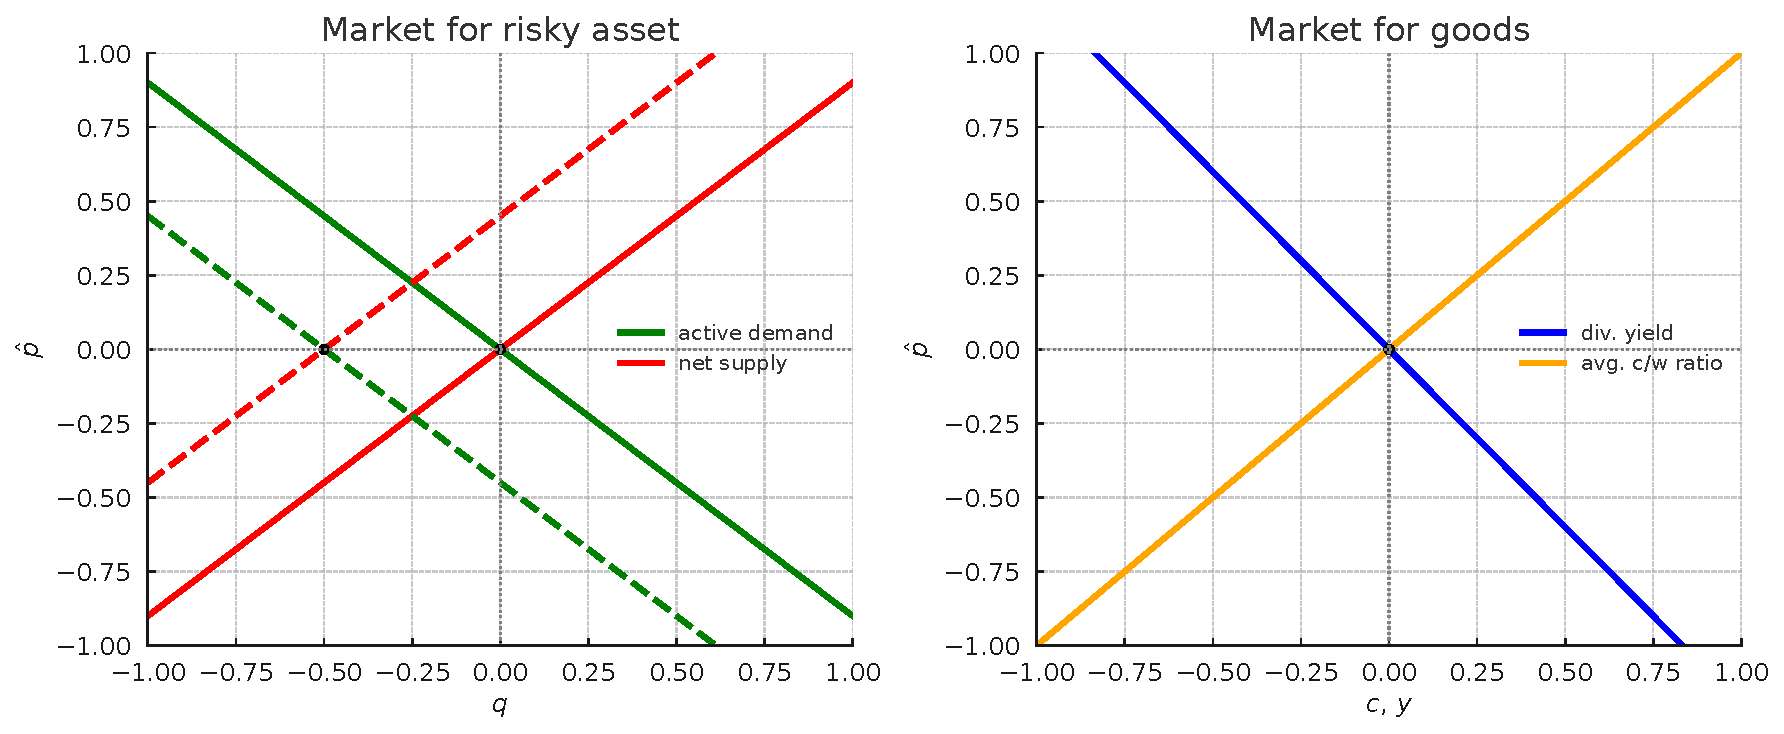
\includegraphics[width=0.95\linewidth]{figures/mkt_equilibrium.pdf}    
    \vspace{2mm}
    \caption{Equilibrium in the risky asset (left) and goods (right) markets.}
    \label{fig:mkt_equilibrium}
\end{figure}

% The left panel of Figure~\ref{fig:mkt_equilibrium} depicts the equilibrium in the market for risky asset. 
% The downward-sloping curve represents the demand from active investors. 
% The upward-sloping curve represents the net supply of risky assets, i.e., the fixed supply minus the demand from passive investors.\footnote{As passive demand is $Q_p = \overline{\alpha}_p [1- c_p(r,\mu-p-r)]\frac{P+Y}{P} Q_p$, the linearized net supply $-Q_p^\star q_p$ will be increasing in $p$ if $c_p(\cdot)$ does not react too strongly to $p$.} 

Linearizing the goods-market condition $\overline{c}(\mu-p)=1/(1+e^{p})$ around $p^\star$ yields
\begin{equation}\label{eq:goods_linear}
    \chi_p\,\hat{p}
    \;=\;
    -\,\frac{e^{p^\star}}{(1+e^{p^\star})^2}\,\hat{p},
    \qquad\text{where}\qquad
    \chi_p \equiv -\,\overline{c}'(\mu-p^\star).
\end{equation}
The right panel of Figure~\ref{fig:mkt_equilibrium} shows the goods market. We focus on the case $\chi_p>0$, so the average consumption-wealth ratio is increasing in $p$ (investors save less when expected returns are low). The right-hand side in \eqref{eq:goods_linear} is the (local) slope of the dividend-yield curve, which is downward sloping in $p$. By the recursive property, only $p$ enters the goods market clearing condition.

% \begin{figure}
%     \centering
%     % \tikzset{every picture/.style={line width=0.75pt}} %set default line width to 0.75pt        

%     \begin{tikzpicture}[x=0.75pt,y=0.75pt,yscale=-1,xscale=1]
%     %uncomment if require: \path (0,235); %set diagram left start at 0, and has height of 235

%     %Shape: Axis 2D [id:dp5132950601646007] 
%     \draw [color={rgb, 255:red, 0; green, 0; blue, 0 }  ,draw opacity=1 ][line width=1.5]  (50,200) -- (289,200)(70,39) -- (70,222) (282,195) -- (289,200) -- (282,205) (65,46) -- (70,39) -- (75,46) (101,195) -- (101,205)(132,195) -- (132,205)(163,195) -- (163,205)(194,195) -- (194,205)(225,195) -- (225,205)(256,195) -- (256,205)(65,169) -- (75,169)(65,138) -- (75,138)(65,107) -- (75,107)(65,76) -- (75,76) ;
%     \draw   ;   
%     %Straight Lines [id:da929233454246288] 
%     \draw [color={rgb, 255:red, 245; green, 166; blue, 35 }  ,draw opacity=1 ][line width=1.5]    (20,56) -- (304,218) ;
%     %Straight Lines [id:da5921961944005785] 
%     \draw [color={rgb, 255:red, 74; green, 144; blue, 226 }  ,draw opacity=1 ][line width=1.5]    (16,200) -- (276,51) ;
%     %Straight Lines [id:da2953578261472096] 
%     \draw [color={rgb, 255:red, 0; green, 0; blue, 0 }  ,draw opacity=1 ][line width=1.5]  [dash pattern={on 1.69pt off 2.76pt}]  (145,126) -- (145,200) ;
%     %Shape: Axis 2D [id:dp3699485075380834] 
%     \draw [color={rgb, 255:red, 0; green, 0; blue, 0 }  ,draw opacity=1 ][line width=1.5]  (380,200) -- (619,200)(400,39) -- (400,222) (612,195) -- (619,200) -- (612,205) (395,46) -- (400,39) -- (405,46) (431,195) -- (431,205)(462,195) -- (462,205)(493,195) -- (493,205)(524,195) -- (524,205)(555,195) -- (555,205)(586,195) -- (586,205)(395,169) -- (405,169)(395,138) -- (405,138)(395,107) -- (405,107)(395,76) -- (405,76) ;
%     \draw   ;
%     %Straight Lines [id:da7483554761171687] 
%     \draw [color={rgb, 255:red, 65; green, 117; blue, 5 }  ,draw opacity=1 ][line width=1.5]    (355,85) -- (638,222) ;
%     %Straight Lines [id:da38811786243247126] 
%     \draw [color={rgb, 255:red, 208; green, 2; blue, 27 }  ,draw opacity=1 ][line width=1.5]    (431,199) -- (460.67,36) ;
%     %Straight Lines [id:da4060861160692876] 
%     \draw [color={rgb, 255:red, 0; green, 0; blue, 0 }  ,draw opacity=1 ][line width=1.5]  [dash pattern={on 1.69pt off 2.76pt}]  (144,127) -- (504.67,127) ;
%     %Straight Lines [id:da3647922931527937] 
%     \draw [color={rgb, 255:red, 65; green, 117; blue, 5 }  ,draw opacity=1 ][line width=1.5]  [dash pattern={on 1.69pt off 2.76pt}]  (372,64.57) -- (655,201.57) ;
%     %Straight Lines [id:da21438260220121663] 
%     \draw [color={rgb, 255:red, 208; green, 2; blue, 27 }  ,draw opacity=1 ][line width=1.5]  [dash pattern={on 1.69pt off 2.76pt}]  (488,200) -- (517.67,37) ;
    
%     % Text Node
%     \draw (231,86) node  [color={rgb, 255:red, 74; green, 144; blue, 226 }  ,opacity=1 ,rotate=-329.57]  {\small $avg.\ c/w\ ratio$};
%     % Text Node
%     \draw (312,201) node  [color={rgb, 255:red, 0; green, 0; blue, 0 }  ,opacity=1 ,rotate=-358.98]  {$c,y$};
%     % Text Node
%     \draw (251,171) node  [color={rgb, 255:red, 245; green, 166; blue, 35 }  ,opacity=1 ,rotate=-28.61]  {\small $div.\ yield$};
%     % Text Node
%     \draw (54,39) node  [color={rgb, 255:red, 0; green, 0; blue, 0 }  ,opacity=1 ,rotate=-358.98]  {$p$};
%     % Text Node
%     \draw (464,63) node  [color={rgb, 255:red, 208; green, 2; blue, 27 }  ,opacity=1 ,rotate=-279.88]  {\small $net\ supply$};
%     % Text Node
%     \draw (630,201) node  [color={rgb, 255:red, 0; green, 0; blue, 0 }  ,opacity=1 ,rotate=-358.98]  {$q$};
%     % Text Node
%     \draw (552,169) node  [color={rgb, 255:red, 65; green, 117; blue, 5 }  ,opacity=1 ,rotate=-25.74]  {\small $active\ demand$};
%     % Text Node
%     \draw (384,39) node  [color={rgb, 255:red, 0; green, 0; blue, 0 }  ,opacity=1 ,rotate=-358.98]  {$p$};
%     % Text Node
%     \draw (107,4.43) node [anchor=north west][inner sep=0.75pt]   [align=left] {\textbf{Market for goods}};
%     % Text Node
%     \draw (435,3) node [anchor=north west][inner sep=0.75pt]   [align=left] {\textbf{Market for risky asset}};
% \end{tikzpicture}
%     \caption{Equilibrium in the goods and risky asset markets}
%     \label{fig:mkt_equilibrium}
% \end{figure}


\paragraph{The inelastic markets hypothesis.}
Consider a \emph{partial equilibrium} version of the model in which we hold the interest rate fixed at $r=r^\star$ and ignore goods market clearing. 
Using the linearized risky asset market condition \eqref{eq:risky_mkt_linear} with $\hat r=0$, the price of the risky asset satisfies
\begin{equation}\label{eq:mkt-elasticity-pe}
    \hat{p}
    \;=\;
    \underbrace{\frac{1}{\zeta_p}}_{\substack{\text{inverse market}\\ \text{elasticity}}}
    \times
    \underbrace{f}_{\text{flow shock}},
\end{equation}
where
\[
\zeta_p \;\equiv\; s_a\,\zeta_{a,p} + s_p\,\zeta_{p,p},
\qquad
f \;\equiv\; s_p\,f_p,
\qquad
s_j \equiv \omega_j Q_j^\star.
\]

Equation~\eqref{eq:mkt-elasticity-pe} shows that the price-dividend ratio responds to flow shocks, with price impact given by the inverse of the (aggregate) market elasticity---an average of investors’ own-price elasticities. This is the core implication of the \emph{inelastic markets hypothesis} of \citet{gabaix2020search}, who estimate large price responses to stock-market flows, suggesting relatively inelastic demand.

In the risky asset panel of Figure~\ref{fig:mkt_equilibrium}, an increase in the portfolio share of passive investors shifts the net supply curve to the left. The new equilibrium lies further up the active demand curve, implying lower expected returns and a higher price-dividend ratio. When demand is inelastic, even small inflows to stocks generate a sizable increase in $\hat{p}$.
% In the risky-asset panel of Figure~\ref{fig:mkt_equilibrium}, a reallocation by passive investors that increases their portfolio share shifts the \emph{net supply} curve to the right. The new intersection moves \emph{down} along active demand, so expected returns must rise and the price-dividend ratio falls. When investors are inelastic, even a small flow away from stocks generates a sizable decline in $\hat{p}$.

\paragraph{The crucial role of cross-elasticity.}
The partial equilibrium analysis abstracts from cross-elasticity. In general equilibrium, however, both $r$ and $p$ adjust, and the aggregate market elasticity is fundamentally different, as the next proposition shows.

\begin{prop}[Infinite market elasticity]\label{prop:inf-elasticity}
    Define the aggregate cross-elasticity $\zeta_r \;\equiv\; s_a\,\zeta_{a,r} \;+\; s_p\,\zeta_{p,r}$.
    If $\zeta_r \neq 0$, then a portfolio-flow shock has \emph{no} price impact: $\hat p=0$. The shock is absorbed by offsetting movements in the interest rate and the risk premium:
    \[
        \hat r \;=\; \frac{1}{\zeta_r}\,f, 
        \qquad 
        \hat \pi \;=\; -\,\frac{1}{\zeta_r}\,f,
    \]
    where $\hat{\pi} \equiv \pi - \pi^\star$.
\end{prop}
\begin{proof}
    From Equation~\eqref{eq:goods_linear}, we obtain $\hat{p} = 0$. 
    If $\zeta_r \neq 0$, then $\hat{r} = \frac{1}{\zeta_r} f$ from Equation~\eqref{eq:risky_mkt_linear}.    
    Since $\hat \pi = -\hat p - \hat r$ with $\hat p=0$, it follows that $\hat \pi = - f/\zeta_r$.
\end{proof}

With any nonzero cross-elasticity $\zeta_r \neq 0$, the aggregate market becomes infinitely elastic, regardless of how inelastic individual demands may be. Even if $\zeta_{j,p}^q \approx 0$ for all $j$, a small but positive $\zeta_r$ is sufficient to make aggregate elasticity unbounded.
%With any nonzero cross-elasticity, $\zeta_r\neq 0$, the market is \emph{infinitely elastic}, regardless of how inelastic individual demands (own-price elasticities) may be. Even if $\zeta_{j,p}^q \approx 0$ for all $j$, a small but positive $\zeta_r$ suffices to make the aggregate elasticity infinite.

The disconnect between individual and aggregate elasticities arises from a general equilibrium effect. In the goods market (right panel of Figure~\ref{fig:mkt_equilibrium}), the price-dividend ratio is determined by consumption behavior. This mechanism is well known in the macro-finance literature, most clearly in models with unit EIS, where $p$ is tied directly to the discount rate. Our framework generalizes this logic. To restore equilibrium in the risky asset market (left panel), the interest rate adjusts so that active demand equals net supply at the \textit{original price}. Graphically, this appears as the dashed active-demand curve shifting to intersect the new net-supply curve at the initial price.
% This disconnect between individual and aggregate elasticities is a result of a general equilibrium effect. In the goods market (right panel of Figure~\ref{fig:mkt_equilibrium}), the price-dividend ratio is pinned down by consumption behavior. 
% This is a pervasive feature in the macro-finance literature, which is most clearly seen in unit EIS models, where $p$ is tied to the discount rate. Our formulation simply extends this logic more broadly. 
% To restore equilibrium in the risky-asset market (left panel), the interest rate adjusts so that active demand meets net supply at the \emph{original} price. In the diagram, this appears as the dashed active-demand schedule shifting until it intersects the new net-supply curve at the initial price.

Consider a positive flow shock to the risky asset (e.g., funds shift toward stocks, so $f>0$). Lower bond demand increases $r$, while increased demand for the risky asset reduces the risk premium. In equilibrium these effects offset exactly, leaving the price-dividend ratio unchanged. If the rise in $r$ were smaller than the fall in the risk premium, there would be excess demand for goods (equivalently, excess bond supply). Simultaneous clearing of risky and risk-free asset markets therefore requires infinite aggregate elasticity in this model.
%Intuitively, consider a negative flow shock to the risky asset (e.g., funds move toward bonds, so $f<0$). The increased bond demand pushes $r$ down, while the reduced demand (or higher net supply) for the risky asset raises the risk premium. In equilibrium these two forces offset \emph{exactly}, leaving the price–dividend ratio unchanged. If the decline in $r$ were too small relative to the increase in the risk premium, there would be excess demand for goods (equivalently, excess bond supply). Simultaneous clearing in the risky and riskless asset markets thus requires infinite aggregate elasticity in this model.

\paragraph{The need for a micro-founded demand system.}
The analysis underscores the central role of cross-price elasticity. The aggregate market can be infinitely elastic—even if individual investors are inelastic—so long as the average consumption-wealth ratio is unaffected by the flow shock $f$. When the flow shock shifts both the net-supply curve and the average consumption-wealth ratio, prices adjust and aggregate elasticity becomes finite.\footnote{An analogous argument applies to uncertainty. With unit EIS, the consumption–wealth ratio is fixed, so higher uncertainty leaves prices unchanged. For uncertainty to reduce prices, EIS must exceed one so that higher uncertainty lowers the consumption–wealth ratio \citep[see][]{bansal2004risks}.}  

Understanding aggregate elasticity therefore requires a framework that links portfolio reallocation shocks to both risky asset demand and bond demand (i.e., savings behavior). To this end, we develop a dynamic heterogeneous-agent asset pricing model and introduce a new methodology for deriving investor demand within this setting.

% The analysis above highlights the central role of cross-price elasticity. It shows that the aggregate market can be infinitely elastic—even when individual investors are inelastic—provided the average consumption-wealth ratio is unchanged by the portfolio flow shock $f$. If the flow shock shifts \emph{both} the net-supply schedule and the average consumption-wealth ratio, prices respond and aggregate elasticity is finite.\footnote{A similar logic applies to changes in uncertainty. When the EIS equals one and the consumption–wealth ratio is fixed, higher uncertainty leaves the price unchanged. For uncertainty to lower the price, a high EIS is required so that higher uncertainty reduces the consumption–wealth ratio (see, e.g., \citealt{bansal2004risks}).}

% Understanding the determinants of aggregate elasticity therefore requires a theory that links portfolio reallocation shocks to \emph{both} risky asset demand and bond demand (i.e., savings behavior). To this end, we develop a dynamic heterogeneous-agent asset pricing model and introduce a new methodology to derive investor demand within this framework.
 

\section{A Dynamic Asset Pricing Model with Passive Investors}\label{sec:model}

This section develops a dynamic heterogeneous-agent asset pricing model that provides a micro-founded demand system.
Building on the framework of Section~\ref{sec:simple}, the economy features both passive and active investors, but now embeds their behavior in a fully dynamic general equilibrium setting.

Passive investors hold exogenously specified, stochastic portfolio shares in risky assets. 
Shocks to their portfolio share generate portfolio-flow (i.e., noisy trading) shocks imperfectly correlated with cash-flow shocks, so the economy is driven by both fundamental and non-fundamental demand disturbances.
Active investors, in contrast, optimally rebalance their portfolios subject to financial frictions.
There are two types of active investors with different risk aversion: a high risk-aversion (unconstrained) investor and a low risk-aversion investor subject to a leverage constraint.

A key extension relative to the simple model is that investors trade two distinct claims—a \emph{dividend claim} (equity) and a \emph{risky corporate bond}—whose payoffs sum to the aggregate endowment.
Explicitly modeling the dividend process allows us to study the response of equity prices to portfolio flows, instead of focusing on the aggregate claim.
% As we show below, this distinction is central: while the aggregate claim remains highly elastic, the dividend claim exhibits large price impact, consistent with the data.
As we show below, this distinction is central, as the price impact for the dividend claim can differ substantially from the price impact for the aggregate claim.

% \section{A Dynamic Asset Pricing Model with Passive Investors}\label{sec:model}

% This section develops a dynamic heterogeneous-agent asset pricing model that provides a micro-founded demand system.
% Building on the framework of Section~\ref{sec:simple}, the economy features both passive and active investors, but now embeds their behavior in a fully dynamic general equilibrium setting.

% Passive investors hold exogenously specified, stochastic portfolio shares in risky assets. 
% Shocks to their portfolio share generate portfolio-flow (i.e., noisy trading) shocks that are imperfectly correlated with cash-flow shocks, so the economy is driven by both fundamental and non-fundamental demand disturbances.
% Active investors, in contrast, continuously rebalance their portfolios subject to financial frictions.
% There are two types of active investors with different risk aversion: a high risk-aversion (unconstrained) investor and a low risk-aversion investor subject to a leverage constraint.

% Relative to the simple model, we allow investors to trade two distinct claims—a \emph{dividend claim} (equity) and a \emph{risky corporate bond}—whose payoffs sum to the aggregate endowment.
% Explicitly modeling the dividend process allows us to study the response of equity prices to portfolio flows, instead of focusing on the aggregate claim.
% As we show below, the market elasticity of the dividend claim can differ substantially from the market elasticity of the aggregate claim.

% A representative firm finances its operations by issuing two types of claims: a \emph{dividend claim} (equity) and a \emph{risky corporate bond}, whose payoffs sum to the aggregate endowment.
% To capture the well-documented fact that dividends are more volatile than consumption (see, e.g., \citealt{Abel1999LeverageDividends}; \citealt{Campbell1999AssetPrices}), we follow \citet{MenzlySantosVeronesi2004} and model the dividend as a mean-reverting stochastic share of output.
% In addition, investors can trade a derivative in zero net supply.
% The derivative plays a key role: by spanning the non-traded Brownian factor, it allows investors to achieve their desired risk exposures without taking asymmetric positions in the individual claims, and is therefore essential for the mutual fund theorem described below.

% A central result of this section is a \emph{mutual fund theorem}: despite access to separate equity and debt claims, all investors optimally hold these claims in proportion to their market-capitalization weights.
% Because the derivative completes markets with respect to the priced sources of risk, investors can adjust their exposure to the non-dividend-share factor through the derivative alone, and optimally hold the risky claims at market-cap weights.
% Consequently, the aggregate equilibrium, including the risk-free rate, risk premia, wealth dynamics, and the stochastic discount factor, is identical to that of an economy with a single claim on aggregate output.
% This separation implies that the perturbation analysis of Section~\ref{sec:elasticity} applies directly to the aggregate equilibrium derived here.
% Individual claim prices are then obtained by solving an auxiliary valuation equation, conditional on the aggregate equilibrium.


\subsection{Environment}

\paragraph{Financial markets.}
We begin by specifying the aggregate endowment process.
The aggregate endowment $Y_t$ follows a geometric Brownian motion:
\begin{equation}\label{eq:agg_endow}
    \frac{dY_t}{Y_t} = \mu\,dt + \sigma\,dZ_t,
\end{equation}
where $\mu \in \mathbb{R}$ and $\sigma \in \mathbb{R}^{1\times d}$ are constants.\footnote{
    Throughout the paper, we adopt the convention that loadings on the Brownian motion are row vectors.
}
The process $Z=\{Z_t\}_{t\ge0}$ is a standard $d$-dimensional Brownian motion on the filtered probability space $(\Omega,\mathcal{F},(\mathcal{F}_t)_{t\ge0},\mathbb{P})$ satisfying the usual conditions.
In the baseline model, $d = 3$, capturing three sources of risk: (i) aggregate endowment shocks, (ii) portfolio-flow shocks to passive investors, and (iii) shocks to the dividend share.
% We focus on the case $\sigma = [\sigma_1, 0, 0]$, so the first shock can be interpreted as a shock to the aggregate endowment.

We consider a representative firm that issues two securities whose payoffs sum to the aggregate endowment.
The first is a \emph{dividend claim} (equity), with payoff flow $D_t = s_t Y_t$.
Following \citet{MenzlySantosVeronesi2004}, the dividend share $s_t \in (0,1)$ follows the mean-reverting process:
\begin{equation}\label{eq:s_process}
    ds_t = \kappa_s(\overline{s} - s_t)\,dt + s_t(1-s_t)\,\sigma_s\,dZ_t,
\end{equation}
given $s_0 \in (0,1)$, with $\overline{s} \in (0,1)$, $\kappa_s > 0$, and $\sigma_s \in \mathbb{R}^{1\times d}$.
This specification ensures $s_t \in [0,1]$ at all times and yields a stationary share process, so consumption and dividends are cointegrated.
As a result, dividends inherit both aggregate risk and additional variation from movements in the dividend share.
By It\^{o}'s lemma, dividends follow:
\begin{equation}\label{eq:D_dynamics}
    \frac{dD_t}{D_t} = \mu_{D,t}\,dt + \sigma_{D,t}\,dZ_t,
\end{equation}
where
\begin{equation}\label{eq:D_vol}
    \sigma_{D,t} = \sigma + (1-s_t)\,\sigma_s, \qquad 
    \mu_{D,t} = \mu + \kappa_s\!\left(\frac{\overline{s}}{s_t}-1\right) + (1-s_t)\,\sigma\sigma_s^\top.
\end{equation}

This specification captures several key features of the data.
First, it generates the well-documented fact that dividends are more volatile than consumption (see, e.g., \citealt{abel1999risk}; \citealt{Campbell1999AssetPrices}).
Second, the dividend share predicts future dividend growth, consistent with \citet{MenzlySantosVeronesi2004}.
Third, dividend volatility increases after negative shocks to $s_t$, capturing a leverage effect.

The second claim is a \emph{corporate bond} (risky debt), with payoff flow $B_t = (1-s_t)Y_t$. 
Since $D_t + B_t = Y_t$, the bond payoff is smoother than aggregate consumption, reflecting the safer nature of debt and its lower exposure to aggregate risk.
This decomposition allows us to distinguish between claims with different risk exposures, with important implications for price impact.

Let $P_{D,t}$ and $P_{B,t}$ denote the ex-dividend prices of the dividend and bond claims, with returns:
\begin{align}
    dR_{D,t} &= \frac{dP_{D,t}+D_t\,dt}{P_{D,t}}
    = \mu_{R_D,t}\,dt+\sigma_{R_D,t}\,dZ_t, \label{eq:RD_def}\\
    dR_{B,t} &= \frac{dP_{B,t}+B_t\,dt}{P_{B,t}}
    = \mu_{R_B,t}\,dt+\sigma_{R_B,t}\,dZ_t. \label{eq:RB_def}
\end{align}
Since $D_t+B_t=Y_t$, the combined claim replicates the aggregate endowment, with price $P_{Y,t} = P_{D,t}+P_{B,t}$. 
The return on the aggregate claim follows:
\begin{equation}\label{eq:risky-asset-ret}
    dR_{Y,t} = \frac{dP_{Y,t}+Y_t\,dt}{P_{Y,t}} = \mu_{R_Y,t}\,dt + \sigma_{R_Y,t}\,dZ_t.
\end{equation}

Investors also have access to a risk-free asset paying rate $r_t$ and, to ensure markets are dynamically complete, a derivative in zero net supply that spans risks not directly traded through the dividend and bond claims. 
In particular, we assume the derivative does not load on dividend-share shocks.
As in a futures contract, there is no initial cash exchange to enter into the derivative contract.
The derivative provides risk exposure $\sigma_{R_F,t} \in \mathbb{R}^{1\times d}$, orthogonal to the aggregate claim, $\sigma_{R_F,t}\,\sigma_{R_Y,t}^\top = 0$, so that it provides independent risk exposure, with normalization $\|\sigma_{R_F,t}\| = \|\sigma_{R_Y,t}\|$.

\paragraph{Stochastic discount factor.} Absence of arbitrage implies the existence of a stochastic discount factor (SDF), $\Lambda_t$, which prices all assets in the economy:
\begin{equation}
    \frac{d\Lambda_t}{\Lambda_t} = -r_t\,dt - \eta_t\,dZ_t,
\end{equation}
where $\eta_t \in \mathbb{R}^{1\times d}$ is the market price of risk vector. 

Absence of arbitrage implies that risk premia satisfy $\pi_{k,t} = \sigma_{R_k,t}\,\eta_t^\top$ for each claim $k \in \{D,B,F\}$.
Let $\Sigma_t$ denote the $3 \times 3$ matrix collecting the risk exposures of all traded assets:
\begin{equation}
    \Sigma_t = \begin{pmatrix}
        \sigma_{R_D,t} \\
        \sigma_{R_B,t} \\
        \sigma_{R_F,t}
    \end{pmatrix},
\end{equation}
and $\pi_t \equiv [\pi_{D,t}, \pi_{B,t}, \pi_{F,t}]^\top$, so that $\pi_t = \Sigma_t\,\eta_t^\top$.

In equilibrium, prices depend on an aggregate state vector $X_t \in \mathbb{R}^N$, so we write $r_t = r(X_t)$, $\eta_t = \eta(X_t)$, and return coefficients as functions of $X_t$. The state vector evolves as
\begin{equation}\label{eq:state_dynamics}
    dX_t = \mu_{X,t}\,dt + \sigma_{X,t}\,dZ_t,
\end{equation}
with drift $\mu_{X,t} \in \mathbb{R}^N$ and exposure matrix $\sigma_{X,t} \in \mathbb{R}^{N\times d}$, both determined in equilibrium.

\paragraph{Demography and preferences.}

The economy consists of three investor types, indexed by $j=0,1,2$, with population mass $\omega_j$: one passive type ($j=0$) and two active types ($j=1,2$). 
Investors die with Poisson intensity $\kappa$, and each instant a mass $\kappa\,\omega_j$ of type-$j$ agents are born, so the total population remains constant and normalized to one. 
Newborns inherit parental wealth, so wealth is redistributed across cohorts without affecting aggregate resources. 
This mortality structure ensures a nondegenerate stationary wealth distribution.

Preferences are recursive as in \citet{duffie1992stochastic}, with type-$j$ risk aversion $\gamma_j$ and a common elasticity of intertemporal substitution (EIS) $\psi$. 
The aggregator is given by:
\begin{equation}
    f_j(C,V) = \rho \frac{(1-\gamma_j) V}{1-\psi^{-1}} 
    \left[ \left( \frac{C}{\big((1-\gamma_j)V\big)^{\frac{1}{1-\gamma_j}}} \right)^{1-\psi^{-1}} - 1 \right],
\end{equation}
% where the discount factor $\rho $ reflects both time impatience $\hat{\rho}$ and the death probability $\kappa$.
where $\rho$ denotes the discount factor.

Each investor chooses consumption $C_{j,t}$ and portfolio allocations across the dividend claim, the bond claim, and the derivative, subject to the constraints specified below.

\paragraph{Passive investors.}
Passive investors allocate a fraction $1-\overline{\alpha}_{p,t}$ of their wealth to the risk-free asset and a fraction $\overline{\alpha}_{p,t}$ to a \textit{market index} fund, which holds the dividend and bond claims in proportion to their market-capitalization weights. 
Passive investors do not trade the derivative.

The share of wealth invested in the market index fund, $\overline{\alpha}_{p,t}$, evolves according to an Ornstein-Uhlenbeck process:
\begin{equation}\label{eq:alpha_p_process}
    d\overline{\alpha}_{p,t}
    \;=\;
    \theta_p\!\left(\overline{\alpha}-\overline{\alpha}_{p,t}\right)\!dt
    \;+\;
    \sigma_{\alpha_p}\,dZ_t,
\end{equation}
with long-run mean $\overline{\alpha}>0$, mean-reversion $\theta_p>0$, and loading $\sigma_{\alpha_p}\in\mathbb{R}^{1\times d}$ on the $d$-dimensional Brownian motion $Z_t$.
Innovations to $\overline{\alpha}_{p,t}$ represent \emph{portfolio flow shocks}, i.e., fluctuations in the fraction of wealth passive investors allocate to risky claims.
As in Section~\ref{sec:simple}, a flow shock is an asymmetric demand shock affecting only passive investors and triggering portfolio reallocation.

Portfolio flows may comove with cash-flow shocks or arise independently. 
We focous on the case where $\sigma=(\sigma_1,0,0)$ for aggregate endowment risk, $\sigma_{\alpha_p}=(\sigma_{\alpha_p,1},\sigma_{\alpha_p,2},0)$ for the passive-share process, and $\sigma_s=(\sigma_{s,1},0,\sigma_{s,3})$ for the dividend share process.
The first shock represents aggregate endowment risk, the second represents portfolio-flow shocks, and the third represents dividend-share shocks.
We allow portfolio-flow shocks and dividend-share shocks to load on the aggregate endowment risk factor.
This implies that aggregate endowment risk can be correlated with both portfolio flows and dividend-share shocks.

The exposure of the passive share to aggregate shocks can reflect \emph{imperfect rebalancing} or \emph{performance-induced flows}. 
Without rebalancing, a positive return on the risky asset mechanically increases the passive share when $\overline{\alpha}_{p,t}<1$. 
Similarly, investors may increase risky exposure after good performance. 
This specification aligns with empirical evidence on passive behavior: households exhibit substantial portfolio inertia \citep{ameriks2011household,brunnermeier2008wealth}; flows chase performance \citep{chevalier1997risk,dannhauser2024flow}; and regulatory changes can sharply increase equity allocations via TDF adoption \citep{parker2022household}, illustrating portfolio flow shocks not tied to cash flow fundamentals.

% We assume passive investors do not trade the derivative, so their portfolio allocations are given by:
% \begin{equation}
%     \alpha_{0,D,t} = \overline{\alpha}_{p,t}\,\omega_{D,t}, \qquad 
%     \alpha_{0,B,t} = \overline{\alpha}_{p,t}\,\omega_{B,t}, \qquad 
%     \alpha_{0,F,t} = 0.
% \end{equation}
% where $\omega_{D,t} \equiv \frac{P_{D,t}}{P_{Y,t}}$ and $\omega_{B,t} \equiv \frac{P_{B,t}}{P_{Y,t}}$ are the market weights of the dividend and bond claims. 


\paragraph{Active investors.} 

Investors of type $j = 1,2$ are \textit{active investors}.
Active investors optimally rebalance their portfolios, choosing allocations across the dividend claim, the bond claim, and the derivative, $\alpha_{j,t} \equiv [\alpha_{j,D,t}, \alpha_{j,B,t}, \alpha_{j,F,t}]^\top$.
Type-2 investors have low risk aversion, $\gamma_2 < \gamma_1$, and therefore have an incentive to lever up their exposure to risky assets.
They borrow short-term to increase their risk exposure, subject to a leverage constraint that limits total portfolio risk:
\begin{equation}\label{eq:leverage_constraint}
    \|\sigma_{j,t}\| \leq \overline{\sigma},
\end{equation}
where $\sigma_{j,t} \equiv \alpha_{j,t}^\top \Sigma_t =  \alpha_{j,D,t}\,\sigma_{R_D,t} + \alpha_{j,B,t}\,\sigma_{R_B,t} + \alpha_{j,F,t}\,\sigma_{R_F,t}$ is the investor's total risk exposure and $\|\cdot\|$ denotes the Euclidean norm.
This constraint resembles a Value-at-Risk (VaR) limit commonly applied to banks and leveraged institutions (see, e.g., \citealt{adrian2014procyclical} and \citealt{brunnermeier2009market}).
Type-1 investors are more risk averse and do not face a leverage constraint.

\paragraph{Investors' problem.}

% An investor of type $j = 0,1,2$ chooses consumption $C_{j,t}$ and portfolio allocations $\alpha_{j,t} \equiv [\alpha_{j,D,t}, \alpha_{j,B,t}, \alpha_{j,F,t}]^\top$ to solve the following problem:
An investor of type $j = 0,1,2$ chooses consumption $C_{j,t}$ and portfolio allocations $\alpha_{j,t}$ to solve the problem:
\begin{equation}\label{eq:inv-problem}
    V_{j,t} = \max_{C_{j,t},\alpha_{j,t}} 
    \mathbb{E}_t \left[ \int_t^\infty f_j(C_{j,s},V_{j,s})\, ds \right], \qquad s.t.
\end{equation}
\begin{equation}\label{eq:budget_constraint}
    \frac{d W_{j,t}}{W_{j,t}} = \left[r_t + \pi_{t}^\top \,\alpha_{j,t} - \frac{C_{j,t}}{W_{j,t}}\right] dt 
    + \sigma_{j,t}\, dZ_t,
\end{equation}
with $W_{j,t} \geq 0$ and $\alpha_{j,t} \in \Omega_{j,t}$,
where $\sigma_{j,t} = \alpha_{j,t}^ \top \Sigma_{t}$ is the investor's risk exposure,
$W_{j,t}$ denotes the investor's wealth, and $\Omega_{j,t}$ is the investment set for type-$j$ investor.

Portfolio allocations are restricted to lie in an \textit{investment set} $\Omega_{j,t}$, which depends on investor type and captures differences in financial constraints across investors.\footnote{
    The differences in investment sets here are reminiscent of the difference in the investment universe emphasized by \citet{Koijen/Yogo/19}.
    }
For passive investors, $j=0$, holdings of the market index fund induce indirect holdings of the dividend and bond claims, so their investment set is given by:
\begin{equation}
    \Omega_{0,t} = \{\alpha_{0,t}:\;
\alpha_{0,D,t} = \overline{\alpha}_{p,t}\, \frac{P_{D,t}}{P_{Y,t}},
\; \alpha_{0,B,t} = \overline{\alpha}_{p,t}\, \frac{P_{B,t}}{P_{Y,t}},
\; \alpha_{0,F,t} = 0\},
\end{equation}

Type-1 investors are unconstrained, so their investment set is given by $\Omega_{1,t} = \mathbb{R}^3$.
For type-$2$ investors, the investment set reflects their leverage constraint:
\begin{equation}
\Omega_{2,t} = \{\alpha_{2,t}: \|\Sigma_t^\top \alpha_{2,t}\| \leq \overline{\sigma}\}.
\end{equation}


\paragraph{Market clearing and equilibrium.}

We define equilibrium as follows.

\begin{defn}
A competitive equilibrium consists of stochastic processes, all adapted to the filtration generated by $Z_t$.
These include the aggregate endowment $Y$, the dividend share $s$, the prices $P_D$ and $P_B$, the risk-free rate $r$, the market price of risk $\eta_t$,
the weight $\overline{\alpha}_p$, and, for each investor $j \in \{0,1,2\}$, wealth $W_j$, consumption $C_j$, and portfolio allocations $\alpha_j$.
These processes satisfy the following conditions:
\begin{enumerate}[label=(\roman*)]

\item The aggregate endowment $Y_t$ evolves according to \eqref{eq:agg_endow}, with $Y_0 > 0$.
The dividend share $s_t$ evolves according to \eqref{eq:s_process}.

\item Given $\{P_{D,t}, P_{B,t}, r_t, \eta_t\}$ and the passive share $\overline{\alpha}_{p,t}$, the choices $(C_{j,t},\alpha_{j,t})$ solve investor $j$'s problem in \eqref{eq:inv-problem}.
The weight on the market index fund, $\overline{\alpha}_{p,t}$, evolves according to \eqref{eq:alpha_p_process}.

\item Markets clear for goods, the dividend and bond claims, riskless bonds, and the derivative:
\begin{equation}
    \sum_{j=0}^2 \omega_j C_{j,t} = Y_t,
    \qquad
    \sum_{j=0}^2 \omega_j Q_{j,k,t} = 1, \qquad 
    \sum_{j=0}^2 \omega_j B_{j,t} = 0,
    \qquad
    \sum_{j=0}^2 \omega_j F_{j,t} = 0,
\end{equation}
for $k \in \{D,B\}$. Holdings are defined as follows.
The number of units of the dividend and bond claims held by investor $j$ are $Q_{j,D,t} = \alpha_{j,D,t} W_{j,t} / P_{D,t}$ and $Q_{j,B,t} = \alpha_{j,B,t} W_{j,t} / P_{B,t}$.
Riskless bond holdings are given by $B_{j,t} = (1 - \alpha_{j,D,t} - \alpha_{j,B,t}) W_{j,t}$.
The notional position in the derivative is $F_{j,t} = \alpha_{j,F,t} W_{j,t}$.\footnote{
    As there is no initial cash exchange for the derivative, wealth invested in the risk-free asset equals total wealth minus the amount invested in the dividend and bond claims.
    }

\end{enumerate}
\end{defn}


\subsection{Equilibrium characterization}\label{sec:equilibrium-char}

We now characterize equilibrium in the dynamic model.
We derive the optimality conditions that govern portfolio choice and consumption decisions, and show how they jointly determine prices and risk premia.
We then establish a version of the \textit{mutual fund theorem} in our economy with frictions.
This result implies that investors hold the dividend and bond claims in proportion to their market-capitalization weights, so that aggregate equilibrium objects are independent of the dividend-share shock.
As a result, the equilibrium admits a \textit{block-recursive} structure, in which we first solve for the aggregate equilibrium and then recover the prices of individual claims.
This representation will be central for our analytical characterization of aggregate market elasticity.

\subsubsection{Equilibrium conditions}

\paragraph{Value function and consumption-wealth ratio.}

With homothetic preferences, investor $j$'s value function can be written as
\begin{equation}
    V_{j,t} = \left( \frac{c_{j,t}}{\rho^\psi} \right)^{\frac{1-\gamma_j}{1-\psi}} 
    \frac{W_{j,t}^{1-\gamma_j}}{1-\gamma_j},
    \qquad
    \text{where} \qquad 
    \frac{dc_{j,t}}{c_{j,t}} = \mu_{c_j,t}\, dt + \sigma_{c_j,t}\, dZ_t.
\end{equation}
The function $c_{j,t} = c_j(X_t)$ denotes the consumption-wealth ratio, so that $C_{j,t}/W_{j,t} = c_{j,t}$.

From the Hamilton-Jacobi-Bellman equation, the consumption-wealth ratio satisfies
\begin{equation}\label{eq:HJB_complete}
    c_{j,t} = \psi \rho 
    + (1-\psi) \left[ r_t + \pi_{t}^\top\,\alpha_{j,t} - \frac{\gamma_j}{2} \|\sigma_{j,t}\|^2 \right] 
    + \xi_{j,t},
\end{equation}
where $\sigma_{j,t} = \alpha_{j,t}^\top \Sigma_t$ is the investor's risk exposure.
The first term reflects time preference, while the second term captures the impact of current investment opportunities on consumption.

The term $\xi_{j,t}$ is given by
\[
    \xi_{j,t} = \mu_{c_j,t} 
    + (1-\gamma_j) \sigma_{c_j,t} \sigma_{j,t}^\top 
    + \frac{\psi - \gamma_j}{1-\psi} \frac{\|\sigma_{c_j,t}\|^2}{2}.
\]
This term captures the effect of changes in future investment opportunities on consumption.

As in Section~\ref{sec:simple}, the consumption-wealth ratio depends on both the interest rate $r_t$ and the risk premium $\pi_t$.
Importantly, it also depends on the investor's portfolio choice $\alpha_{j,t}$.
Finally, $\xi_{j,t}$ acts as a state-dependent shifter, and it is equal to zero when investment opportunities are constant.

\paragraph{Optimal risk exposure share.}
The optimal risk exposure for active investors $j = 1,2$ is given by
\begin{equation}
    \sigma_{j,t}
    = \frac{1}{1+\nu_{j,t}} \left[ \frac{\eta_t}{\gamma_j} + \frac{1-\gamma_j^{-1}}{\psi-1} \, \sigma_{c_j,t} \right],
\end{equation}
where $\nu_{j,t}$ is the Lagrange multiplier on the leverage constraint, so $\nu_{j,t} \ge 0$ and $\nu_{1,t} = 0$.
When the leverage constraint is not binding, the optimal risk exposure is the sum of two components.
The first is the myopic demand, $\frac{\eta_t}{\gamma_j}$, which depends on the investor's risk tolerance and the vector of market prices of risk $\eta_t$.
This term captures the compensation per unit of exposure to each risk factor: $\eta_t^\top = \Sigma_t^{-1} \pi_t$.
The second is the hedging demand, $\frac{1-\gamma_j^{-1}}{\psi-1} \, \sigma_{c_j,t}$, which reflects the investor's desire to hedge fluctuations in future investment opportunities.
When the constraint binds, the multiplier $\nu_{j,t} > 0$ scales down exposure uniformly across all risk factors to satisfy $\|\sigma_{j,t}\| \le \overline{\sigma}$.
This acts like an endogenous increase in effective risk aversion.

The Lagrange multiplier $\nu_{2,t}$ satisfies the complementary slackness condition:
\begin{equation}
    \nu_{2,t} \left( \|\sigma_{2,t}\| - \overline{\sigma} \right) = 0.
\end{equation}

For passive investors, risk exposure is given by
\begin{equation}
    \sigma_{0,t} = \overline{\alpha}_{p,t} \sigma_{R_Y,t},
\end{equation}
where $\sigma_{R_Y,t}$ is the risk exposure of the market index fund.
Hence, $\overline{\alpha}_{p,t}$ contols the overall risk exposure of passive investors.

Given an investor's risk exposure, the corresponding portfolio shares are recovered from
\[
\alpha_{j,t} = \left(\sigma_{j,t} \, \Sigma_t^{-1}\right)^\top,
\]
which maps risk exposures into asset holdings.

\paragraph{Market clearing conditions.}

Market clearing implies that aggregate wealth equals the price of the aggregate claim:
\begin{equation}
    \sum_{j=0}^2 \omega_j W_{j,t} = P_{Y,t}.
\end{equation}

Let $x_{j,t}$ denote the wealth share of type-$j$ investors:
\begin{equation}\nonumber
    x_{j,t} \equiv \frac{\omega_j W_{j,t}}{P_{Y,t}}.
\end{equation}

The market clearing conditions for goods and risky assets are given by:
\begin{equation}
    \sum_{j=0}^2 x_{j,t} c_{j,t} = \frac{1}{p_{Y,t}},
    \qquad \qquad 
    \sum_{j=0}^2 x_{j,t} \sigma_{j,t} = \sigma_{R_Y,t}.
\end{equation}

These conditions echo those in the simple model. 
The first condition states that the wealth-weighted average consumption-wealth ratio equals the dividend yield of the aggregate claim.
The second condition states that the wealth-weighted average risk exposure equals the risk exposure of the economy's endowment claim.
% These conditions summarize equilibrium in terms of aggregate objects, and will allow us to characterize prices and risk premia using the distribution of wealth across investors.

% \paragraph{Market price of risk.} 
% We can write the market clearing condition for risky assets as follows:
% \begin{equation}
%     \underbrace{\sum_{j=1}^2 \frac{x_{j,t}}{x_{a,t}} \sigma_{j,t}}_{\substack{\text{active demand} \\ \text{for risk}}}, = \underbrace{\chi_{a,t} \sigma_{R_Y,t}}_{\substack{\text{net supply} \\ \text{of risk}}}, 
% \end{equation}
% where $\chi_{a,t} \equiv \frac{1- x_{0,t} \overline{\alpha}_{p,t}}{1-x_{0,t}}$ captures the fraction of risk held by active investors, and
% $x_{a,t} \equiv 1-x_{0,t}$ is the wealth share of active investors.

% The expression above shows that the demand from active investors equals the net supply of risky assets to active investors, captured by the total supply minus the demand from passive investors.

% Using the optimal risk exposure, we can solve for the market price of risk:
% \begin{equation}\label{eq:market_price_of_risk}
%     \eta_t = \gamma_{a,t} \left[\chi_{a,t}\sigma_{R_Y,t} - h_{a,t}\right],
% \end{equation}
% where $h_{a,t} \equiv \sum_{j=1}^2 \frac{x_{j,t}}{x_{a,t}} \frac{1-\gamma_j^{-1}}{\psi-1} \, \frac{\sigma_{c_j,t}}{1+\nu_{j,t}}$ is the average hedging demand of active investors adjusted for leverage constraints, and $\gamma_{a,t}$ is the average effective risk aversion of active investors:
% \begin{equation}
%     \gamma_{a,t} \equiv \left[\sum_{j=1}^2 \frac{x_{j,t}}{x_{a,t}} \frac{1}{\gamma_j(1+\nu_{j,t})}\right]^{-1}.
% \end{equation}

% Equation~\eqref{eq:market_price_of_risk} shows that the market price of risk depends on three factors. 
% First, the average effective risk aversion of active investors, $\gamma_{a,t}$. 
% This will vary over time with the wealth shares of active investors, $x_{j,t}$, and the extent leverage constraints bind, as captured by the Lagrange multipliers $\nu_{j,t}$.
% Second, the fraction of risk held by active investors, $\chi_{a,t}$.
% As passive investors hold more of the market index fund, the fraction of risk held by active investors falls, reducing the compensation for risk.
% Third, the average hedging demand of active investors, $h_{a,t}$.
% Intuitively, an increase in the average hedging demand of active investors reduces the compensation for risk.

\paragraph{Market price of risk.} 

We can write the market clearing condition for risky assets as follows:
\begin{equation}
    \underbrace{\sum_{j=1}^2 \frac{x_{j,t}}{x_{a,t}} \sigma_{j,t}}_{\substack{\text{active demand} \\ \text{for risk}}}
    =
    \underbrace{\chi_{a,t} \sigma_{R_Y,t}}_{\substack{\text{net supply} \\ \text{of risk}}},
\end{equation}
where $\chi_{a,t} \equiv \frac{1- x_{0,t} \overline{\alpha}_{p,t}}{1-x_{0,t}}$ captures the share of aggregate risk that must be absorbed by active investors, and $x_{a,t} \equiv 1-x_{0,t}$ is the wealth share of active investors.

This is the dynamic counterpart of the risk market clearing condition in Section~\ref{sec:simple}.
The expression above states that active investors absorb the net supply of risk, defined as total risk minus the portion held by passive investors.

Substituting optimal risk exposures into the market clearing condition yields the market price of risk:
\begin{equation}\label{eq:market_price_of_risk}
    \eta_t = \gamma_{a,t} \left[\chi_{a,t}\sigma_{R_Y,t} - h_{a,t}\right],
\end{equation}
where $h_{a,t} = \sum_{j=1}^2 \frac{x_{j,t}}{x_{a,t}} \frac{1-\gamma_j^{-1}}{\psi-1} \, \frac{\sigma_{c_j,t}}{1+\nu_{j,t}}$ is the average hedging demand of active investors, adjusted for leverage constraints, and $\gamma_{a,t}$ is the average effective risk aversion:
\begin{equation}
    \gamma_{a,t} \equiv \left[\sum_{j=1}^2 \frac{x_{j,t}}{x_{a,t}} \frac{1}{\gamma_j(1+\nu_{j,t})}\right]^{-1}.
\end{equation}

Equation~\eqref{eq:market_price_of_risk} shows that the market price of risk is determined by three forces.

First, the average effective risk aversion of active investors, $\gamma_{a,t}$.
This varies over time with the wealth distribution and the extent to which leverage constraints bind.

Second, the net supply of risk to active investors, captured by $\chi_{a,t}\sigma_{R_Y,t}$.
As passive investors increase their holdings of the market index, the amount of risk that must be absorbed by active investors falls, reducing the compensation for risk.

Third, the average hedging demand of active investors, $h_{a,t}$.
Higher hedging demand implies active investors are willing to bear more risk, lowering the equilibrium compensation for risk.

Equation~\eqref{eq:market_price_of_risk} makes clear that portfolio flows affect risk premia through their impact on the net supply of risk absorbed by active investors.

\paragraph{Interest rate.}
Combining goods market clearing with the expression for the consumption--wealth ratio yields the equilibrium interest rate:
\begin{align}\label{eq:interest_rate}
    r_t &= \rho 
    + \psi^{-1} \left(\mu_{P_Y,t} + \xi_t \right)
    + (1-\psi^{-1}) \sum_{j=0}^2 x_{j,t} 
        \frac{\gamma_j}{2} \|\sigma_{j,t}\|^2
    - \pi_{Y,t},
\end{align}
where $\xi_t \equiv \sum_{j=0}^2 x_{j,t} \, \xi_{j,t}$.

The first term reflects time preference.
The second term captures intertemporal substitution.
The third term and fourth terms capture the effect of uncertainty on the interest rate.

This expression highlights that the interest rate is determined jointly by risk premia and the allocation of risk across investors, providing the key general equilibrium link between portfolio flows, risk allocation, and saving behavior.


\paragraph{Pricing condition.}

Let $p_{D,t} \equiv P_{D,t}/D_{t}$ and $p_{B,t} \equiv P_{B,t}/B_{t}$ denote the price-dividend ratios of the dividend and corporate bond claims, respectively. 
The price-dividend ratio of the aggregate claim is $p_{Y,t} \equiv P_{Y,t}/Y_t$, which satisfies $p_{Y,t} = s_t p_{D,t} + (1-s_t) p_{B,t}$.

The pricing condition for each claim $k$ is given by
\begin{equation}\label{eq:pricing_cond}
    \frac{1}{p_{k,t}} = r_t + \pi_{k,t} - \big(\mu_{k,t} + \mu_{p_k,t} + \sigma_{k,t} \, \sigma_{p_k,t}^\top\big),
\end{equation}
where $\pi_{k,t} = \sigma_{R_k,t} \, \eta_t^\top$ is the risk premium on claim $k$ implied by no arbitrage.
The terms $\mu_{p_k,t}$ and $\sigma_{p_k,t}$ denote the drift and diffusion of the price-dividend ratio, respectively.

% Equation~\eqref{eq:pricing_cond} links asset prices to expected returns, risk premia, and the dynamics of valuation ratios.
% It provides the key condition determining how prices respond to changes in investment opportunities.

\paragraph{State variables.}

The aggregate state vector consists of both endogenous and exogenous variables.
The endogenous state variables are the wealth shares of active investors, $x_{1,t}$ and $x_{2,t}$, which summarize the distribution of wealth.
The exogenous state variables are the passive portfolio share $\overline{\alpha}_{p,t}$ and the dividend share $s_t$.

Hence, the aggregate state vector is $X_t = (x_t, \overline{\alpha}_{p,t}, s_t)$, where $x_t = (x_{1,t}, x_{2,t})$.
The processes $\overline{\alpha}_{p,t}$ and $s_t$ evolve according to \eqref{eq:alpha_p_process} and \eqref{eq:s_process}, respectively.
To obtain $\mu_{X,t}$ and $\sigma_{X,t}$, we need to solve for the drift and diffusion of the endogenous state variables, $x_{1,t}$ and $x_{2,t}$.

By It\^{o}'s lemma, the law of motion for $x_{j,t}$ is given by
\begin{align*}
    \frac{dx_{j,t}}{x_{j,t}} 
    &= \Big[ (\eta_t-\sigma_{R_Y,t}) \left( \sigma_{j,t} -\sigma_{R_Y,t} \right)^\top - \left( c_{j,t} - \frac{1}{p_{Y,t}}  \right)
        + \kappa \frac{\omega_j - x_{j,t}}{x_{j,t}} \Big] dt  
        + (\sigma_{j,t} - \sigma_{R_Y,t}) \, dZ_t.
\end{align*}

% This expression shows that wealth shares evolve with relative returns, consumption decisions, and exposure to aggregate shocks.
% The final term reflects mean reversion due to the demographic structure.


% The aggregate state is $X_t = (x_t, \overline{\alpha}_{p,t})$, where $x_t = (x_{1,t}, x_{2,t}, \ldots, x_{J,t})$ and $\overline{\alpha}_{p,t}$ evolves as in \eqref{eq:alpha_p_process}. By It\^{o}'s lemma, the law of motion for $x_{j,t}$ is
% \begin{align*}
%     \frac{dx_{j,t}}{x_{j,t}} 
%     &= \Big[ r_t + \pi_t \alpha_{j,t} - c_{j,t} - \mu_{P,t} 
%         + (1-\alpha_{j,t}) \|\sigma_{R,t}\|^2 
%         + \kappa \frac{\omega_j - x_{j,t}}{x_{j,t}} \Big] dt  + (\alpha_{j,t} - 1)\, \sigma_{R,t}\, dZ_t.
% \end{align*}

% \paragraph{Risk premium and interest rate.} 

% Let $\mathcal{J}_t^u$ and $\mathcal{J}_t^c$ denote the sets of unconstrained and constrained active investors at time $t$, with wealth shares $x_{u,t} \equiv \sum_{j\in \mathcal{J}_t^u} x_{j,t}$ and $x_{c,t} \equiv \sum_{j\in \mathcal{J}_t^c} x_{j,t}$. From market clearing for the risky asset, demand from unconstrained investors satisfies
% \begin{equation}\label{eq:mkt-clearing}
%     \underbrace{\sum_{j \in \mathcal{J}_t^u} x_{j,t} \alpha_{j,t} }_{\substack{\text{unconstrained active demand}}} = \underbrace{1 - x_{0,t} \overline{\alpha}_{p,t} - x_{c,t} \overline{\alpha}_{c,t} }_{\text{net supply}},
% \end{equation}
% where $\overline{\alpha}_{c,t} \equiv \overline{\sigma}/\|\sigma_{R,t}\|$ is the portfolio share of constrained agents.

% Combining this condition with the optimal portfolios yields the risk premium:
% \begin{equation}\label{eq:sharpe_ratio}
%     \pi_t = \frac{\gamma_{u,t} \|\sigma_{R,t}\|^2}{x_{u,t}}
%     \left[ 1 - x_{0,t}\, \overline{\alpha}_{p,t} 
%     - x_{c,t}\, \overline{\alpha}_{c,t} 
%     - x_{u,t}\, \varsigma_t \right],
% \end{equation}
% where $\gamma_{u,t} \equiv [\sum_{j\in\mathcal{J}_t^u} \frac{x_{j,t}}{x_{u,t}} \frac{1}{\gamma_j}]^{-1}$ is the average risk aversion and $\varsigma_t \equiv \sum_{j\in \mathcal{J}_t^u} \frac{x_{j,t}}{x_{u,t}} \varsigma_{j,t}$ the average hedging demand of unconstrained investors.  
% Equation~\eqref{eq:sharpe_ratio} shows that the risk premium rises with higher risk aversion, lower passive demand, tighter leverage constraints, or weaker hedging motives.

% Goods market clearing requires
% \begin{equation}
%     \sum_{j=0}^J x_{j,t} c_{j,t} = \frac{1}{p_t}.
% \end{equation}
% Combining this with \eqref{eq:xi_j} gives the equilibrium interest rate:
% \begin{align}\label{eq:interest_rate}
%     r_t &= \rho + \psi^{-1} (\mu_{P,t} + \xi_t )
%     + (1-\psi^{-1}) \sum_{j=0}^J x_{j,t} 
%         \frac{\gamma_j \alpha_{j,t}^2}{2} \|\sigma_{R,t}\|^2
%     - \pi_t,
% \end{align}
% where $\xi_t \equiv \sum_{j=0}^J x_{j,t} \xi_{j,t}$.  
% The first two terms reflect impatience and intertemporal substitution, while the third term captures precautionary savings.

% \paragraph{Optimal portfolio and derivative exposure.} 
% An active investor chooses $\alpha_{j,t}$ to maximize the right-hand side of \eqref{eq:HJB_complete} subject to $\|\sigma_{j,t}\|\le\overline{\sigma}$. 
% Let $\nu_{j,t}\ge 0$ denote the Lagrange multiplier on the leverage constraint. The first-order conditions imply
% \begin{equation}\label{eq:foc_eta}
%     \eta_{j,t} = \eta_t,
% \end{equation}
% where $\eta_{j,t} \equiv \gamma_j \left[\Sigma_{j,t} + \frac{1 - \gamma_j^{-1}}{1-\psi} \sigma_{c_j,t}\right] + \frac{\nu_{j,t}}{1-\psi} \Sigma_{j,t}$ is investor $j$'s marginal price of risk. That is, each investor's marginal valuation of risk is equalized to the market price of risk $\eta_t$.

\paragraph{Endogenous volatility.} 

Return volatility has both a cash-flow and a valuation component, $\sigma_{R_k,t} = \sigma_{k,t} + \sigma_{p_k,t}$, where $\sigma_{k,t}$ reflects cash-flow volatility and $\sigma_{p_k,t}$ arises from movements in the price-dividend ratio $p_{k,t}$ for asset $k \in \{D,B\}$. 
By It\^{o}'s lemma,  
\begin{equation}\label{eq:_endogenous_vol}
    \sigma_{p_k,t} = \frac{p_{k,x}(X_t)}{p_{k,t}(X_t)} \sigma_{x,t} 
    + \frac{p_{k,\overline{\alpha}_p}(X_t)}{p_{k,t}(X_t)} \sigma_{\overline{\alpha}_p,t} 
    + \frac{p_{k,s}(X_t)}{p_{k,t}(X_t)} \sigma_{s,t}.
\end{equation}

Equation~\eqref{eq:_endogenous_vol} shows that endogenous volatility depends on the sensitivity of the price-dividend ratio to three groups of variables: (i) the wealth distribution, (ii) the passive portfolio share, and (iii) the dividend share.
The first term is standard in heterogeneous-agent models \citep[see][]{panageas2020implications}.
The third term is typical of models with multiple assets.
The second term arises only in the presence of exogenous portfolio flow shocks.
This second term is quantitatively important when markets are sufficiently inelastic, that is, when price-dividend ratios are highly sensitive to changes in passive demand.
Thus, \eqref{eq:_endogenous_vol} provides a direct link between market elasticity and return volatility, as lower elasticity amplifies the sensitivity of prices to portfolio flows and therefore increases endogenous volatility.

Given the volatility of individual claims, the volatility of the aggregate claim follows from aggregation:
\[
\sigma_{R_Y,t} = \sum_{k=D,B} \frac{P_{k,t}}{P_{Y,t}} \sigma_{R_{k},t}.
\]

It remains to determine $\sigma_{R_F,t}$.  
We make three assumptions about $\sigma_{R_F,t}$:
(i) it does not load on the dividend-share shock, so $\sigma_{R_F,t,3} = 0$;
(ii) it is orthogonal to the aggregate claim, so $\sigma_{R_F,t}\,\sigma_{R_Y,t}^\top = 0$;
(iii) it has the same norm as the aggregate claim, so $\|\sigma_{R_F,t}\| = \|\sigma_{R_Y,t}\|$. 
These conditions uniquely determine $\sigma_{R_F,t}$ given $\sigma_{R_Y,t}$.

\paragraph{Markov equilibrium.} 

Equations \eqref{eq:market_price_of_risk} and \eqref{eq:interest_rate} allow us to express the market price of risk $\eta_t$ and the interest rate $r_t$ as functions of the consumption-wealth ratios $c_j(X_t)$ and the valuation ratios $p_k(X_t)$.
Using It\^{o}'s lemma, the drift and diffusion terms $(\mu_{c_j,t}, \mu_{p_k,t})$ and $(\sigma_{c_j,t}, \sigma_{p_k,t})$ can be written as functions of the state dynamics $(\mu_{X,t}, \sigma_{X,t})$.

Substituting these expressions into the HJB equation \eqref{eq:HJB_complete} and the pricing condition \eqref{eq:pricing_cond}, together with the laws of motion for the state variables, yields a system of five partial differential equations.

These equations jointly determine the consumption-wealth ratios $\{c_j(X_t)\}_{j=0}^2$ and the price-dividend ratios $\{p_k(X_t)\}_{k \in \{D,B\}}$ as functions of four state variables:
the two active wealth shares $x_{1,t}$ and $x_{2,t}$, the passive portfolio share $\overline{\alpha}_{p,t}$, and the dividend share $s_t$.

\subsubsection{Block recursivity and the mutual fund theorem}\label{sec:pricing_claims}

We show that the system of PDEs admits a block-recursive structure.
First, we solve for the consumption-wealth ratios and the price-dividend ratio of the aggregate claim in a reduced set of states $\hat{X}_t = (x_{1,t}, x_{2,t}, \overline{\alpha}_{p,t})$.
Second, we solve for the price-dividend ratios of the dividend and corporate bond claims in the full set of states $X_t = (x_{1,t}, x_{2,t}, \overline{\alpha}_{p,t}, s_t)$.
% This separation arises because aggregate quantities are independent of the dividend-share shock and market are dynamically complete.

This provides a substantial simplification, as the equilibrium allocation and pricing kernel are identical to those of an economy with a single claim on the aggregate endowment and a derivative.
At the same time, the block-recursive structure allows us to recover the pricing implications for individual claims.
In particular, we can characterize how portfolio flows affect the market elasticity of the dividend claim.

An important implication of the block-recursive structure is that a version of the \textit{mutual fund theorem} holds in our economy.
Despite financial frictions, investors optimally hold risky claims in proportion to their market-capitalization weights, as in the classic mutual fund theorem.

\begin{prop}[Block recursivity and the mutual fund theorem]\label{prop:mft}
    Define the reduced set of states as $\hat{X}_t = (x_{1,t}, x_{2,t}, \overline{\alpha}_{p,t})$. Then,
    \begin{enumerate}[label=(\roman*)]
        \item \textbf{Block recursivity:} The consumption-wealth ratios, $\{c_{j,t}(\hat{X}_t)\}_{j=0}^2$, and the price-dividend ratio for the aggregate claim, $p_Y(\hat{X}_t)$, are a function of the reduced set of states $\hat{X}_t$, and they satisfy the following system of PDEs:
        \begin{align}
            c_{j} &= \psi \rho 
            + (1-\psi) \left[ r + \eta^\top\,\sigma_{j} - \frac{\gamma_j}{2} \|\sigma_{j}\|^2 \right] 
            +  \mu_{c_j} 
            + (1-\gamma_j) \sigma_{c_j} \sigma_{j}^\top 
            + \frac{\psi - \gamma_j}{1-\psi} \frac{\|\sigma_{c_j}\|^2}{2}\\
            \frac{1}{p_{Y}} &= r + \eta^\top\,(\sigma + \sigma_{p_Y}) - \big(\mu + \mu_{p_Y} + \sigma \, \sigma_{p_Y}^\top\big),        
    \end{align}
    where $(r, \eta, \sigma_{j}, \mu_{c_j}, \sigma_{c_j}, \mu_{p_Y}, \sigma_{p_Y})$ are all functions of $\hat{X}_t$, $(c_j,p_Y)$ and their derivatives.    
        \item \textbf{Mutual fund theorem:} The portfolio shares of active investors are given by:
        \begin{align}
            \alpha_{j,k} = \alpha_{j,Y} \frac{P_k}{P_Y}, \quad \forall k \in \{D,B\},
        \end{align}
        where $\alpha_{j,Y}$ denotes the holdings of the market index fund for investor $j$, which satisfies the condition
        \begin{equation}
            \sigma_{j} = \alpha_{j,Y} \sigma_{R_Y} + \alpha_{j,F} \sigma_{R_F}.
        \end{equation}
    \end{enumerate}
\end{prop}

Proposition~\ref{prop:mft} shows that the equilibrium with separate dividend and bond claims is equivalent to that of an economy with a single claim on the aggregate endowment and a derivative.

Two assumptions are key to this result.
First, the aggregate endowment process $Y_t$ is independent of the dividend share $s_t$.
This assumption follows \citet{MenzlySantosVeronesi2004}, but differs from the two-trees model of \citet{cochraneLongstaffSantaClara2008}, where the dividend share affects aggregate volatility.

Second, markets are dynamically complete.
In equilibrium, investors are not exposed to the dividend-share shock, which can be perfectly diversified by holding the dividend and bond claims in proportion to their market-capitalization weights.
Investors can therefore obtain any desired exposure to the fundamental and portfolio-flow shocks by trading the market index fund and the derivative.

Without the derivative, investors would need to deviate from market-capitalization weights to adjust their exposure to these risks, at the cost of bearing dividend-share risk.

\paragraph{Pricing the individual claims.}
Having solved for the aggregate objects $\{c_{j,t}(\hat{X}_t)\}_{j=0}^2$ and $p_Y(\hat{X}_t)$, we next recover the valuation of individual claims.
The price-dividend ratios of the dividend and bond claims are functions of the full state vector $X_t = (x_{1,t}, x_{2,t}, \overline{\alpha}_{p,t}, s_t)$, as they load on the dividend-share shock.

Given the aggregate equilibrium objects $r(\hat{X}_t)$ and $\eta(\hat{X}_t)$, and using It\^{o}'s lemma to express the drift and diffusion of valuation ratios as functions of the state dynamics and their derivatives, the pricing condition in Equation~\eqref{eq:pricing_cond} yields a linear PDE for $p_{D,t}(X_t)$ and $p_{B,t}(X_t)$.

Thus, individual claim prices are obtained in a second step, conditional on the aggregate equilibrium.
This separation highlights that portfolio flows affect aggregate quantities through the reduced state vector, while their impact on individual asset prices operates through valuation in the full state space.

This completes the characterization of the equilibrium with separate dividend and bond claims.
We now turn to an analytical characterization of the aggregate market elasticity in this economy.

% \paragraph{Mutual fund theorem.}
% The availability of three tradable assets (the dividend claim, the bond claim, and the derivative) raises the question of whether the decomposition of the aggregate endowment into separate claims affects equilibrium allocations. The following proposition shows that it does not.

% \begin{prop}[Mutual fund theorem]\label{prop:mft}
% Let $(c_{j,t}^*, \alpha_{j,t}^*, \theta_{j,t}^*)$ denote the equilibrium allocation in the economy with a single claim on the aggregate endowment and a derivative. Then the equilibrium of the economy with separate dividend and bond claims is given by:
% \begin{enumerate}[label=(\roman*)]
%     \item $c_{j,t} = c_{j,t}^*$ for all $j$;
%     \item $\alpha_{j,D,t} = \omega_{D,t}\,\alpha_{j,t}^*$ and $\alpha_{j,B,t} = \omega_{B,t}\,\alpha_{j,t}^*$ for all active $j$;
%     \item $\theta_{j,t} = \theta_{j,t}^*$ for all $j$.
% \end{enumerate}
% All investors hold the dividend and bond claims in market-capitalization weights.
% \end{prop}

% The proof proceeds by verification. Under the conjectured allocation, each investor's total risk exposure becomes $\Sigma_{j,t} = \alpha_{j,t}^*\,\sigma_{R_Y,t} + \theta_{j,t}^*\,\sigma_{R_F,t}$, which has zero loading on the dividend-share shock (the third Brownian component). Since the risk premium on the aggregate claim satisfies $\pi_{Y,t} = \omega_{D,t}\,\pi_{D,t} + \omega_{B,t}\,\pi_{B,t}$ and the aggregate return exposure satisfies $\sigma_{R_Y,t} = \omega_{D,t}\,\sigma_{R_D,t} + \omega_{B,t}\,\sigma_{R_B,t}$, it follows that $c_{j,t} = c_{j,t}^*$ satisfies the HJB equation. The first-order conditions and all market clearing conditions are also satisfied, as the value-weighted sum of market-cap-weighted claims replicates the aggregate endowment.

% Proposition~\ref{prop:mft} has two important implications. First, the stochastic discount factor, risk-free rate, and aggregate risk premium depend only on the aggregate state $X_t$ and are independent of the dividend share $s_t$. The perturbation analysis of Section~\ref{sec:elasticity} therefore applies directly to the aggregate equilibrium. Second, individual claim prices can be computed in a second step, by solving a valuation equation conditional on the aggregate equilibrium, as described in Section~\ref{sec:pricing_claims}.

% In light of Proposition~\ref{prop:mft}, we characterize the aggregate equilibrium in terms of the total risky share $\alpha_{j,t} \equiv \alpha_{j,D,t} + \alpha_{j,B,t}$, the risk premium on the aggregate claim $\pi_t \equiv \mu_{R_Y,t} - r_t$, and the return exposure $\sigma_{R,t} \equiv \sigma_{R_Y,t}$.

% \paragraph{Optimal portfolio share.}
% The optimal total risky share for an active investor is
% \begin{equation}\label{eq:portfolio_share}
%     \alpha_{j,t} = \min \left\{ 
%         \frac{\pi_t}{\gamma_j \|\sigma_{R,t}\|^2} + \varsigma_{j,t}, \,
%         \frac{\overline{\sigma}}{\|\sigma_{R,t}\|} 
%     \right\},
% \end{equation}
% where $\varsigma_{j,t} \equiv \frac{1-\gamma_j^{-1}}{\psi-1} 
% \dfrac{\sigma_{c_j,t} \sigma_{R,t}^\top}{\|\sigma_{R,t}\|^2}$ is the hedging component. The myopic demand, $\frac{\pi_t}{\gamma_j \|\sigma_{R,t}\|^2}$, reflects the investor's risk tolerance, while the hedging demand captures the covariance between $c_{j,t}$ and risky returns. The leverage constraint caps exposure at $\overline{\sigma}/\|\sigma_{R,t}\|$.

% From the Hamilton-Jacobi-Bellman equation, the consumption-wealth ratio is
% \begin{equation}\label{eq:xi_j}
%     c_{j,t} = \psi \rho 
%     + (1-\psi) \left[ r_t + \pi_t \alpha_{j,t} 
%         - \frac{\gamma_j}{2} \|\sigma_{R,t}\|^2 \alpha_{j,t}^2 \right] 
%     + \xi_{j,t},
% \end{equation}
% where 
% \[
%     \xi_{j,t} \equiv \mu_{c_j,t} 
%     + (1-\gamma_j) \sigma_{c_j,t} \sigma_{R,t}^\top \alpha_{j,t} 
%     + \frac{\psi - \gamma_j}{1-\psi} \frac{\|\sigma_{c_j,t}\|^2}{2}
% \]
% is a forward-looking term capturing how expected shifts in $c_{j,t}$ affect consumption choices.
% The consumption--wealth ratio depends both on current investment opportunities, summarized by $r_t + \pi_t \alpha_{j,t} - \frac{\gamma_j}{2} \alpha_{j,t}^2 \|\sigma_{R,t}\|^2$, and on future opportunities, summarized by $\xi_{j,t}$. 

% By Proposition~\ref{prop:mft}, the stochastic discount factor depends only on the aggregate state $X_t$ and is independent of the dividend share $s_t$. Individual claim prices can therefore be determined in a second step, conditional on the equilibrium objects $r(X_t)$ and $\eta(X_t)$ from the aggregate economy.

% Let $\hat{X}_t = (X_t, s_t)$ denote the extended state vector. Define the valuation ratio of claim $k \in \{D,B\}$ as $p_{k,t} \equiv P_{k,t}/Y_t = p_k(X_t,s_t)$. Since $P_{k,t} = p_{k,t}\,Y_t$, the return on claim $k$ satisfies
% \begin{equation}
%     \sigma_{R_k,t} = \sigma + \sigma_{p_k,t}, \qquad 
%     \mu_{R_k,t} = \frac{s_{k,t}}{p_{k,t}} + \mu + \mu_{p_k,t} + \sigma\,\sigma_{p_k,t}^\top,
% \end{equation}
% where $s_{D,t} = s_t$, $s_{B,t} = 1-s_t$, and the diffusion of the valuation ratio is
% \begin{equation}
%     \sigma_{p_k,t} = \frac{1}{p_{k,t}}\!\left(p_{k,X}\,\sigma_X + p_{k,s}\,\sigma_s\right),
% \end{equation}
% with $p_{k,X} \equiv \frac{\partial p_k}{\partial X}$ and $p_{k,s} \equiv \frac{\partial p_k}{\partial s}$. Substituting into the pricing condition $\mu_{R_k,t} - r_t = \sigma_{R_k,t}\,\eta_t^\top$ yields the partial differential equation for the valuation ratio $p_k(X,s)$:
% \begin{align}\label{eq:pde_claim}
% 0 =\;&\, p_{k,X}\,\mu_X + p_{k,s}\,\mu_s 
% + \frac{1}{2}\Big[\mathrm{tr}\!\left(\sigma_X\sigma_X^\top\,p_{k,XX}\right) + 2\,p_{k,Xs}\,(\sigma_X\sigma_s^\top) + (\sigma_s\sigma_s^\top)\,p_{k,ss}\Big] \nonumber\\
% &- (r(X)-\mu)\,p_k(X,s) + s_k(s) \nonumber\\
% &+ p_k(X,s)\,\sigma\,\sigma_{p_k}(X,s)^\top - p_k(X,s)\,\sigma\,\eta(X)^\top - p_k(X,s)\,\sigma_{p_k}(X,s)\,\eta(X)^\top.
% \end{align}
% This equation can be solved numerically given the equilibrium functions $r(X)$ and $\eta(X)$ from the aggregate economy. Since $p_{D}(X,s) + p_{B}(X,s) = p(X)$ by construction, only one of the two claim prices needs to be solved independently.

% \section{The Determinants of the Aggregate Market Elasticity}\label{sec:elasticity}

% In this section, we analyze how the \textit{aggregate market elasticity} shapes how portfolio flows affect asset prices. 
% The elasticity is determined by the coupled PDE system \eqref{eq:xi_j}–\eqref{eq:pricing_cond}, which generally admits no closed-form solution. 
% To understand its determinants, we extend the perturbation method of \citet{kogan2001risk} and derive asymptotic closed-form expressions for the elasticity.
In this section, we analyze how the \emph{aggregate market elasticity} governs the price impact of portfolio flows.  
The elasticity is determined by the coupled PDE system \eqref{eq:xi_j}–\eqref{eq:pricing_cond}, which generally has no closed-form solution. To study its determinants, we extend the perturbation method of \citet{kogan2001risk} and derive asymptotic closed-form approximations.

\paragraph{State-global perturbations}

Our perturbation approach studies economies in a neighborhood of a benchmark that admits a closed-form solution.
% A convenient benchmark consists of the case where there is no preference heterogeneity, $\gamma_j = \gamma$, and passive investors are fully invested in the risky asset, $\overline{\alpha}_{p,t} = 1$. 
% In this case, we effectively obtain a Lucas economy, as shown in the next lemma. 
% Throughout, a superscript $*$ denotes the benchmark economy.
A convenient benchmark arises when preferences are homogeneous, $\gamma_j=\gamma$, and passive investors are fully invested in the risky asset, $\overline{\alpha}_{p,t}=1$. In this case, the economy collapses to a Lucas economy, as shown in Lemma~\ref{lemma:benchmark}. Throughout, a superscript $*$ denotes benchmark values.



\begin{lemma}[Benchmark economy]\label{lemma:benchmark}
Suppose $\gamma_j = \gamma$, $\overline{\alpha}_{p,t} = 1$, and $\rho>\big(1-\psi^{-1}\big)\big(\mu - \frac{\gamma \|\sigma\|^2}{2}\big)$. Then, 
\begin{equation}
        \pi^* = \gamma \|\sigma\|^2, \qquad 
        r^* = \rho + \psi^{-1}\mu - \big(1+\psi^{-1}\big)\frac{\gamma \|\sigma\|^2}{2}, \qquad 
        p^* = \Big[\rho - \big(1-\psi^{-1}\big)\Big(\mu - \frac{\gamma \|\sigma\|^2}{2}\Big)\Big]^{-1},
\end{equation}
$c_{j}^* = (p^*)^{-1}$, and $\alpha_{j}^* = 1$ for $j = 0, \ldots, J$.
\end{lemma}

We analyze small deviations from this benchmark. Formally, consider a family of economies indexed by $\epsilon>0$, where $\epsilon$ scales departures from the benchmark along the following dimensions.

First, investors have heterogeneous risk aversion:
\begin{equation}\label{eq:gamma-perturb}
    \gamma_j=\gamma\big(1+\hat{\gamma}_j\epsilon\big), 
    \qquad
    \sum_{j=0}^J \omega_j \hat{\gamma}_j=0,
\end{equation}
so that $\gamma$ is the population-weighted average and $\hat{\gamma}_j$ measures deviations. When $\epsilon=0$, preferences are homogeneous; when $\epsilon=1$, we recover the heterogeneous-investor economy.

% Second, passive investors need not be fully invested in the risky asset. We write their portfolio share as  
% \begin{equation}\label{eq:apbar_index}
%     \overline{\alpha}_{p,t} \;=\; 1 + \hat{\alpha}_{p,t}\,\epsilon,
% \end{equation}
% where $\hat{\alpha}_{p,t}$ captures deviations from the benchmark of full investment and evolves according to an Ornstein-Uhlenbeck process, consistent with Equation~\eqref{eq:alpha_p_process}.% Second, the passive investor may not be fully invested in the risky asset:
% \begin{equation}\label{eq:apbar_index}
%     \overline{\alpha}_{p,t}=1+\hat{\alpha}_{p,t}\,\epsilon,
% \end{equation}
% where $\hat{\alpha}_{p,t}$, which governs deviations from the benchmark, follows an Ornstein-Uhlenbeck process, consistent with Equation~\eqref{eq:alpha_p_process}. 

% For simplicity, we abstract from time variation in passive portfolios and take $\hat{\alpha}_p$ as constant. In this case $Z_t$ is one-dimensional and we set $\sigma\equiv\|\sigma\|$.

Second, passive investors need not be fully invested in the risky asset. Their portfolio share is  
\begin{equation}\label{eq:apbar_index}
    \overline{\alpha}_{p,t}=1+\hat{\alpha}_{p,t}\,\epsilon,
\end{equation}
where $\hat{\alpha}_{p,t}$ measures deviations from full investment benchmark and evolves as an Ornstein-Uhlenbeck process, consistent with Equation~\eqref{eq:alpha_p_process}.

% We also assume the leverage-constraint coefficient satisfies
% \begin{equation}\label{eq:sig_bar-perturb}
%     \overline{\sigma}=\sigma\left(1+\hat{\sigma}\,\epsilon\right),
% \end{equation}
% so that the tightness of the constraint is $\mathcal{O}(\epsilon)$, matching the order of leverage demand. Finally, we assume the mortality parameter is small: $\kappa=\hat{\kappa}\,\epsilon$.

Third, the leverage constraint coefficient is perturbed according to
\begin{equation}\label{eq:sig_bar-perturb}
    \overline{\sigma}=\|\sigma\|\big(1+\hat{\sigma}\,\epsilon\big),
\end{equation}
so that the tightness of the constraint is of order $\mathcal{O}(\epsilon)$, matching the order of leverage demand. Finally, we assume a small mortality rate, $\kappa=\hat{\kappa}\,\epsilon$.

% Equilibrium objects now depend on both the state $X_t$ and the parameter $\epsilon$. We expand them to second order in $\epsilon$:
% \begin{align}
%     p(X,\epsilon) &= p_0(X) + p_1(X)\epsilon + p_2(X)\epsilon^2 + \mathcal{O}(\epsilon^3), \\
%     c_j(X,\epsilon) &= c_{j,0}(X) + c_{j,1}(X)\epsilon + c_{j,2}(X)\epsilon^2 + \mathcal{O}(\epsilon^3),
% \end{align}
% where $p_k(X)$ and $c_{j,k}(X)$, $k\in \{0,1,2\}$, are functions of the state $X$.  

% Unlike standard DSGE perturbations, which linearize in both $X$ and $\epsilon$, our method is \emph{state-global}: we solve directly for functions of $X$ rather than local coefficients around a steady state.\footnote{A formal comparison with standard perturbation methods is provided in \citet{kargar2020competitive}.}
% We refer to this approach as a \textit{state-global perturbation}.\footnote{The method follows the perturbation approach of \citet{kogan2001risk} and builds on the extension of \citet{Silva/riskchannel} to economies with passive investors.}
% This allows us to characterize how the aggregate market elasticity varies with the state of the economy.

% We proceed in two steps: first, we characterize the first-order corrections $p_1(X)$ and $c_{j,1}(X)$; second, we solve for the second-order terms $p_2(X)$ and $c_{j,2}(X)$. The zeroth-order terms $p_0(X)$ and $c_{j,0}(X)$ are given by Lemma~\ref{lemma:benchmark}, that is, $p_0(X) = p^*$ and $c_{j,0}(X) = c_j^*$.
Equilibrium objects now depend on both the state $X_t$ and the parameter $\epsilon$. We expand them to second order:
\begin{align}
    p(X,\epsilon) &= p_0(X) + p_1(X)\epsilon + p_2(X)\epsilon^2 + \mathcal{O}(\epsilon^3), \\
    c_j(X,\epsilon) &= c_{j,0}(X) + c_{j,1}(X)\epsilon + c_{j,2}(X)\epsilon^2 + \mathcal{O}(\epsilon^3),
\end{align}
where $p_k(X)$ and $c_{j,k}(X)$, $k\in\{0,1,2\}$, are functions of the state $X$.

Unlike standard DSGE perturbations, which linearize in both $X$ and $\epsilon$, our method is \emph{state-global}: we solve directly for functions of $X$ rather than coefficients around a steady state.\footnote{See \citet{kargar2020competitive} for a comparison with standard perturbation methods.} 
We refer to this approach as a \emph{state-global perturbation}. 
This approach builds on the perturbation method of \citet{kogan2001risk} and, more closely, the extension 
by \citet{Silva/riskchannel}.
This method allows us to characterize how aggregate market elasticity varies with the state of the economy.

We proceed in two steps. First, we compute the first-order corrections $p_1(X)$ and $c_{j,1}(X)$. Second, we solve for the second-order terms $p_2(X)$ and $c_{j,2}(X)$. Zeroth-order terms are given by Lemma~\ref{lemma:benchmark}, i.e., $p_0(X)=p^*$ and $c_{j,0}(X)=c_j^*$.


% \subsubsection{The benchmark economy}

% In the absence of preference heterogeneity, and with passive investors fully invested in the risky asset, the economy effectively behaves as the frictionless Lucas economy with a representative agent. 

% \begin{lemma}[Benchmark economy]\label{lemma:benchmark}
% Suppose $\rho>\left(1-\psi^{-1}\right)\left( \mu - \frac{\gamma
% \sigma^2}{2}  \right)$.\footnote{The condition $\rho>\left(1-\psi^{-1}\right)\left( \mu - \frac{\gamma
% \sigma^2}{2}  \right)$ is standard in economies with growth and risk, guaranteeing that investors achieve finite utility.} Then, for the $\epsilon=0$ economy, 
% \begin{enumerate}[(i)]
% \item Investors' consumption-wealth ratio and risk exposure are given by:
% \begin{equation}
%  c_{j,0}(X) = \rho - \left(1-\psi^{-1}\right) \left( \mu - \frac{\gamma \sigma^2}{2} \right), \qquad \alpha_{j,0}(X) = 1, \qquad \text{for } j = 0,1,\ldots, J.\nonumber
% \end{equation}

% \item Risk premium, risk-free rate, and price-dividend ratio are given by:
% \begin{equation}\nonumber
%     \pi_0 (X) = \gamma \sigma^2, \qquad 
%     r_0(X) = \rho + \psi^{-1} \mu - \left (1+\psi^{-1}\right ) \frac{\gamma \sigma^2}{2}, \qquad 
%     p_0(X) =  \frac{1}{c_{j,0}(X)}.
% \end{equation}
% \end{enumerate}
% \end{lemma}
% \begin{proof}
% See Appendix~\ref{app:lemma1}.
% \end{proof}

% Lemma~\ref{lemma:benchmark} shows that there is no time variation in the expected returns in the benchmark economy in the absence of frictions. 
% In particular, the price-dividend ratio $p_0(X)$ is constant in the benchmark economy, so the risk premium and interest rate are given by the standard Lucas economy formulae.
% % Moreover, the return volatility is equal to the volatility of dividends since the price-dividend ratio $p_0(X)$ is constant in this case.

% \paragraph{The benchmark economy.}

% When preferences are homogeneous and passive investors are fully invested in the risky asset ($\epsilon=0$), the economy reduces to the frictionless Lucas representative-agent benchmark.  

% \begin{lemma}[Benchmark economy]\label{lemma:benchmark}
% Suppose $\rho>\big(1-\psi^{-1}\big)\big(\mu - \frac{\gamma \sigma^2}{2}\big)$,\footnote{This condition is standard in models with growth and risk and ensures finite utility.} then in the $\epsilon=0$ economy:
% \begin{enumerate}[(i)]
%     \item Consumption–wealth ratios and portfolio shares are
%     \[
%         c_{j,0}(X) = \rho - \big(1-\psi^{-1}\big)\Big(\mu - \frac{\gamma \sigma^2}{2}\Big), 
%         \qquad \alpha_{j,0}(X) = 1, 
%         \qquad j=0,1,\ldots,J.
%     \]
%     \item Risk premium, interest rate, and price–dividend ratio are
%     \[
%         \pi_0(X) = \gamma \sigma^2, \qquad 
%         r_0(X) = \rho + \psi^{-1}\mu - \big(1+\psi^{-1}\big)\frac{\gamma \sigma^2}{2}, \qquad 
%         p_0(X) = \frac{1}{c_{j,0}(X)}.
%     \]
% \end{enumerate}
% \end{lemma}
% \begin{proof}
% See Appendix~\ref{app:lemma1}.
% \end{proof}

% Lemma~\ref{lemma:benchmark} implies that in the absence of frictions, expected returns are constant: the price–dividend ratio $p_0(X)$ is fixed, and the risk premium and interest rate coincide with the standard Lucas economy formulas.


% \subsection{The first-order demand system}

% We consider next the first-order approximation of the demand system. 
% Investor $j$'s demand for the risky asset is given by $Q_{j}(X;\epsilon) = \alpha_{j}(X;\epsilon) \frac{x_{j}}{\omega_{j}}.$ 
% Let $q_{j,t} = \log Q_{j,t} / Q_{j,0}(X_t)$ denote the log deviation of investor $j$'s demand from her demand in the benchmark economy. Up to first order, we can write $q_{j,t}$ as follows:
% \begin{equation}
%     q_{j,t} = \alpha_{j,1}(X_t) \epsilon + \mathcal{O}(\epsilon^2),
% \end{equation}
% where $\alpha_{j,1}(X_t) $ is the first-order correction for portfolio weight $\alpha_j(X;\epsilon)$. Three observations are important in computing $\alpha_{j,1}$. First, the endogenous volatility is equal to zero up to first order, as $\sigma_{p,t}$ is given by 
% \begin{equation}
%     \sigma_{p,t} = \frac{p_x(X_t)}{p(X_t)} \sigma_x(X_t) = \left[ \frac{p_{x,1}(X_t)}{p_0(X_t)} \sigma_{x,0}(X_t) +\frac{p_{x,0}(X_t)}{p_0(X_t)} \sigma_{x,1}(X_t) \right] \epsilon + \mathcal{O}(\epsilon^2) = \mathcal{O}(\epsilon^2),
% \end{equation}
% where $p_{x,0}(X_t) = \sigma_{x,0}(X_t) = 0$, as shown in Lemma \ref{lemma:benchmark}. Second, the hedging demand is also second-order in $\epsilon$, $\varsigma_{j,t} = \mathcal{O}(\epsilon^2)$,
% as a similar argument shows that $\sigma_{c_j}(X_t) = \mathcal{O}(\epsilon^2)$. Third, expanding the pricing condition \eqref{eq:pricing_cond}, we obtain the analogous of Equation \eqref{eq: risk_premium}:
% \begin{equation}
% \hat{\pi}_t = - \hat{r}_t - \frac{1}{p^*} \hat{p}_t + \mathcal{O}(\epsilon^2),
% \end{equation}
% where $\hat{\pi}_t \equiv \pi_t - \pi_0(X_t)$, $\hat{r}_t \equiv r_t - r_0(X_t)$, and $\hat{p}_t = \frac{p_t - p^*}{p^*}$, using the fact that $\mu_{p,t} = \mathcal{O}(\epsilon^2)$ and $p^* \equiv p_0(X)$. 
% As in Section \ref{sec:simple}, we can use the pricing condition to write the risk premium in terms of the price-dividend ratio and the interest rate.

% Using the three observations above, we can compute the first-order expansion of the portfolio share in Equation \eqref{eq:portfolio_share} to obtain investor $j$'s demand for an unconstrained investor :
% \begin{equation}\label{eq:demand_risky}
%     q_{j,t} = -\zeta^q_{j, p} \hat{p}_t - \zeta^q_{j,r} \hat{r}_t + f_{j,t} + \mathcal{O}(\epsilon^2), 
% \end{equation}
% where $$\zeta_{j,p}^q \equiv \frac{1}{p^*} \frac{1}{\gamma \sigma^2}, \qquad \zeta_{j,r}^q \equiv \frac{1}{\gamma \sigma^2}, \qquad f_{j,t} \equiv -\hat{\gamma}_j \epsilon.$$ 
% A similar equation holds for a constrained investor, but in this case $\zeta_{j,p}^q = \zeta_{j,r}^q = 0$ and $f_{j,t} = \frac{\hat{\sigma}}{\|\sigma\|} \epsilon$. 
% The demand from passive investors also takes the form above, with $\zeta_{0,p}^q = \zeta_{0,r}^q = 0$, and $f_{0,t} = \hat{\alpha}_{p} \epsilon$.

% The demand for the risky asset for unconstrained agents is analogous to the active demand in Section~\ref{sec:simple}. 
% However, we can now relate the elasticities to the underlying parameters. 
% The price elasticity $\zeta_{j,p}^q$ is given by $\frac{1/p^*}{\gamma \sigma^2}$, the ratio of the dividend yield and the risk premium in the benchmark economy, while the cross price-elasticity $\zeta_{j,r}^q$ is given by the inverse of the risk premium.  Importantly, the cross price-elasticity is non-zero for unconstrained investors. 
% As shown above, the direct and cross price elasticities are equal to zero for a constrained investor. 
% Finally, even if $\hat{r}_t = \hat{\pi}_t = 0$, investors' demand would deviate from the one in the benchmark economy due to differences in risk aversion, the leverage limit, or the passive portfolio. 
% These effects are captured by the demand shifters $f_{j,t}$.

% We can proceed in an analogous way to compute the first-order expansion of the consumption-wealth ratio in Equation~\eqref{eq:xi_j}:
% \begin{equation}
%     c_{j,t} = \psi \rho + (1-\psi) \left[ r_t + \pi_t  - \frac{\gamma_j \sigma^2}{2}  \right] + \mathcal{O}(\epsilon^2),
% \end{equation}
% where we used the fact that $\xi_t = \mathcal{O}(\epsilon^2)$. 
% % Consistent with Assumption \ref{assump:c_w_property}, the risk-free rate and the risk premium affect in the same way the consumption-wealth ratio up to first order. 
% In line with Assumption~\ref{assump:c_w_property}, both the risk-free rate and risk premium have a similar first-order impact on the consumption-wealth ratio.
% Using the pricing condition, we can write $\hat{c}_{j,t} \equiv c_{j,t} - c_{j,0}(X_t)$ in terms of $\hat{p}_t$ and a shifter:
% \begin{equation}
%     \hat{c}_{j,t} = \zeta^c_{j,p} \hat{p}_t + \zeta^c_{j,0},
% \end{equation}
% where $\zeta_{j,p}^c \equiv (\psi-1) \frac{1}{p^*}$ and $\zeta^c_{j,0} \equiv (\psi-1) \frac{\gamma \sigma^2}{2} \hat{\gamma}_j \epsilon$.
% Notice that the consumption-wealth ratio does not depend on $r_t$ given $p_t$, as in Section \ref{sec:simple}.
% The consumption-wealth ratio can be either increasing or decreasing in $p_t$.
% The case depicted in Figure \ref{fig:mkt_equilibrium}, where the consumption-wealth ratio is increasing in $p_t$, corresponds to $\psi > 1$, a common assumption in macro-finance models (see e.g. \citealt{bansal2004risks}).
% Another important property is that the consumption-wealth ratio is independent of $\overline{\alpha}_{p,t}$, which has implications for the determination of the market elasticity.


\subsection{The first-order demand system}

\paragraph{Demand for risky asset.}  
Investor $j$’s demand for the risky asset is 
\[
    Q_j(X;\epsilon)=\alpha_j(X;\epsilon)\,\frac{x_j}{\omega_j},
\]
where $x_j$ is the wealth share. Define the proportional deviation from the benchmark as
\begin{equation}
    q_{j,t}\;\equiv\;\frac{Q_j(X_t;\epsilon)- Q_j(X_t;0)}{Q_j(X_t;0)}
    \;=\;\alpha_{j,1}(X_t)\,\epsilon+\mathcal{O}(\epsilon^2),
\end{equation}
where $\alpha_{j,1}(X)$ is the first-order correction to the portfolio weight.  

Three results determine $\alpha_{j,1}(X)$. First, the volatility of the price-dividend ratio is second order:
\[
    \sigma_{p,t}=\frac{p_X(X_t)}{p(X_t)}\,\sigma_X(X_t)=\mathcal{O}(\epsilon^2),
\]
since $p_{X,0}=\sigma_{X,0}=0$ (Lemma~\ref{lemma:benchmark}). Second, hedging demand is also $\mathcal{O}(\epsilon^2)$ because $\sigma_{c_j}(X_t)$ is second order. Third, expanding the pricing condition \eqref{eq:pricing_cond} gives
\begin{equation}
    \hat{\pi}_t=-\,\hat{r}_t-\frac{1}{p^*}\hat{p}_t+\mathcal{O}(\epsilon^2),
\end{equation}
where $\hat{\pi}_t\equiv \pi_t-\pi^*$, $\hat{r}_t\equiv r_t-r^*$, and $\hat{p}_t\equiv \frac{p_t-p^*}{p^*}$, using $\mu_{p,t}=\mathcal{O}(\epsilon^2)$.

Substituting into \eqref{eq:portfolio_share}, the first-order demand system is
\begin{equation}\label{eq:demand_risky}
    q_{j,t}=-\,\zeta_{j,p}\,\hat{p}_t-\zeta_{j,r}\,\hat{r}_t+f_{j,t}+\mathcal{O}(\epsilon^2),
\end{equation}
where, for unconstrained investors,
\[
    \zeta_{j,p}=\frac{1}{p^*}\frac{1}{\gamma\|\sigma\|^2}, 
    \qquad
    \zeta_{j,r}=\frac{1}{\gamma\|\sigma\|^2}, 
    \qquad
    f_{j,t}=-\,\hat{\gamma}_j\,\epsilon.
\]
For passive and constrained investors, own- and cross-price elasticities vanish, $\zeta_{j,p}=\zeta_{j,r}=0$, with demand shifters $f_{j,t}=\hat{\sigma}\,\epsilon$ for constrained investors and $f_{0,t}=\hat{\alpha}_{p,t}\,\epsilon$ for passive investors.  

Equation~\eqref{eq:demand_risky} shows that the first-order approximation to the dynamic heterogeneous agent model in Section~\ref{sec:model} provides microfoundations for the demand system in Section~\ref{sec:simple}. As in the simple model, unconstrained active investors exhibit nonzero own- and cross-price elasticities, here explicitly linked to structural parameters. Shocks to $\overline{\alpha}_{p,t}$ move the passive investors’ demand shifter $f_{0,t}$—the dynamic analog of the comparative statics in Section~\ref{sec:simple}. In addition, the model generates further demand shifts from occasionally binding leverage constraints faced by active investors.

% \paragraph{Consumption-wealth ratio.}
% Similarly, the first-order expansion of \eqref{eq:xi_j} for consumption yields
% \begin{equation}
%     c_{j,t}
%     \;=\;
%     \psi\rho \;+\; (1-\psi)\!\left[r_t + \pi_t - \frac{\gamma_j\sigma^2}{2}\right]
%     \;+\; \mathcal{O}(\epsilon^2).
% \end{equation}
% In line with Assumption~\ref{assump:c_w_property}, the risk-free rate and the risk premium have the same first-order impact on the consumption–wealth ratio. Using the expansion
% \(\hat\pi_t = -\,\hat r_t - p^{*\, -1}\hat p_t + \mathcal{O}(\epsilon^2)\), we obtain
% \begin{equation}
%     \hat c_{j,t} \;\equiv\; c_{j,t} - c_{j}^*
%     \;=\; \chi_{j,0} \;+\; \chi_{j,p}\,\hat p_t \;+\; \mathcal{O}(\epsilon^2),
% \end{equation}
% with
% $    \chi_{j,p} \;\equiv\; (\psi-1)\,\frac{1}{p^*},$ 
%     and
%     $\chi_{j,0} \;\equiv\; (\psi-1)\,\frac{\gamma\sigma^2}{2}\,\hat{\gamma}_j\,\epsilon.
% $


% Hence, conditional on \(p_t\), the consumption–wealth ratio is independent of \(r_t\), as in Section~\ref{sec:simple}. Its slope with respect to \(p_t\) depends on the EIS: it is increasing in \(p_t\) when \(\psi>1\), as in standard macro-finance models \citep{bansal2004risks}. Finally, the consumption–wealth ratio is independent of \(\overline{\alpha}_{p,t}\) to first order, a fact that will matter for aggregate market elasticity.

\paragraph{Consumption-wealth ratio.}  
A first-order expansion of \eqref{eq:xi_j} yields
\begin{equation}
    c_{j,t}
    \;=\;
    \psi\rho \;+\; (1-\psi)\!\left[r_t + \pi_t - \frac{\gamma_j\|\sigma\|^2}{2}\right]
    \;+\; \mathcal{O}(\epsilon^2).
\end{equation}
Consistent with Assumption~\ref{assump:c_w_property}, the risk-free rate and the risk premium enter symmetrically at first order. Substituting the expansion
\(\hat{\pi}_t = -\,\hat{r}_t - p^{*\,-1}\hat{p}_t + \mathcal{O}(\epsilon^2)\) gives
\begin{equation}
    \hat c_{j,t} \;\equiv\; c_{j,t} - c_j^*
    \;=\; \chi_{j,0} \;+\; \chi_{j,p}\,\hat{p}_t \;+\; \mathcal{O}(\epsilon^2),
\end{equation}
with coefficients
\[
    \chi_{j,p}=(\psi-1)\,\frac{1}{p^*},
    \qquad 
    \chi_{j,0}=(\psi-1)\,\frac{\gamma\|\sigma\|^2}{2}\,\hat{\gamma}_j\,\epsilon.
\]

Hence, conditional on $p_t$, the consumption-wealth ratio is independent of $r_t$, as in Section~\ref{sec:simple}. Its slope with respect to $p_t$ depends on the EIS: it rises with $p_t$ when $\psi>1$, the standard assumption in macro-finance models. Finally, to first order, the consumption–wealth ratio is unaffected by $\overline{\alpha}_{p,t}$, a property that will be central for aggregate market elasticity.

% \subsubsection{Aggregate market elasticity in frictionless economies}

% Given the demand system, we can solve for the equilibrium prices. The market clearing conditions for the risky asset and for goods can be written as
% \begin{equation}
%     \sum_{j=0}^J x_{j} q_{j,t} = 0, \qquad \qquad 
%     \sum_{j=0}^J x_{j} \hat{c}_{j,t} = -\frac{1}{p^*} \hat{p}_t,\nonumber
% \end{equation}

% Aggregating the demand for the risky asset and the consumption-wealth ratio, we obtain
% \begin{equation}
%     \left[
%     \begin{matrix}
%         \zeta^q_p & \zeta^q_r\\
%         \zeta^c_p + \frac{1}{p^*} & 0
%     \end{matrix}
%     \right]\left[ \begin{matrix}
%         \hat{p}_t\\
%         \hat{r}_t
%     \end{matrix} \right] =
%     \left[ \begin{matrix}
%         f_t\\
%         -\zeta_{0}^c
%     \end{matrix} \right],\nonumber
% \end{equation}
% where $\zeta^q_{k} \equiv \sum_{j=0}^J x_j \zeta_{j,k}^q$, for $k \in \{p,r\}$, $\zeta^c_{k} \equiv \sum_{j=0}^J x_j \zeta^c_{j,k}$, for $k \in \{p,0\}$, and $f_t \equiv \sum_{j=0}^J x_j f_{j,t}$.

% Solving the system above, we obtain asset prices in this economy: 
% \begin{equation}
%     \hat{p}_t = - \frac{\zeta_0^c}{\zeta_p^c + \frac{1}{p^*} }, \qquad \qquad 
%     \hat{r}_t = \frac{f_t}{\zeta_r^q} + \frac{\zeta_p^q}{\zeta_r^q \left( \zeta_p^c + \frac{1}{p^*} \right)} \zeta_0^c.\nonumber
% \end{equation}

% The aggregate market elasticity, $\epsilon_{M,t}$, is defined as the inverse of the proportional change in the price of the risky asset in response to a portfolio flow shock $f_t$:
% \begin{equation}
%     \epsilon_{M,t}^{-1} = \left( \frac{\partial \hat{p}_t}{\partial f_t} \right)^{-1}.\nonumber
% \end{equation}

% As $\hat{p}_t$ is independent of the portfolio flow shock $f_t$, the inverse elasticity is equal to zero up to first order:
% \begin{equation}
%     \epsilon_{M,t}^{-1} = 0.
% \end{equation}
% This result echoes the findings in Section \ref{sec:simple} which showed how the aggregate elasticity could be infinite in the context of a two-period economy. We obtain the same result now in the context of our dynamic economy using a first-order approximation.

\paragraph{Aggregate market elasticity.}  
Given the demand system, equilibrium prices follow from market clearing in the risky-asset and goods markets:
\[
    \sum_{j=0}^J x_{j,t}\, q_{j,t} = 0,
    \qquad
    \sum_{j=0}^J x_{j,t}\, \hat{c}_{j,t} = -\frac{1}{p^*}\,\hat{p}_t .
\]

Aggregating across investors, and dropping the $j$ subscript on coefficients that are common across types, yields the linear system
\[
    \begin{bmatrix}
        \zeta_p & \zeta_r \\
        \chi_p + \tfrac{1}{p^*} & 0
    \end{bmatrix}
    \begin{bmatrix}
        \hat{p}_t \\[4pt]
        \hat{r}_t
    \end{bmatrix}
    =
    \begin{bmatrix}
        f_t \\[4pt]
        -\,\chi_{0,t}
    \end{bmatrix},
\]
where $f_t \equiv \sum_{j=0}^J x_{j,t} f_{j,t}$ and $\chi_{0,t} \equiv \sum_{j=0}^J x_j \chi_{j,0}$.

\begin{defn}[Aggregate market elasticity]
The aggregate market elasticity $\epsilon_{M,t}$ is defined as the inverse of the proportional change in the price of the risky asset in response to a flow shock $f_t$:
\[
    \epsilon_{M,t} \;\equiv\; \Big[\,\frac{\partial \hat{p}_t}{\partial f_t}\,\Big]^{-1}.
\]
\end{defn}

\begin{prop}[First-order impact of portfolio flows]\label{prop:first_order}
Suppose $\rho>\big(1-\psi^{-1}\big)\big(\mu - \tfrac{\gamma\|\sigma\|^2}{2}\big)$. Then:
\begin{enumerate}[label=(\roman*)]
    \item The price impact is zero to first order:
    \(
        \epsilon_{M,t}^{-1}=\frac{\partial \hat{p}_t}{\partial f_t}=0 .
    \)
    \item The interest rate and risk premium responses satisfy
    \[
        \frac{\partial \hat{r}_t}{\partial f_t}=\frac{1}{\zeta_r},
        \qquad
        \frac{\partial \hat{\pi}_t}{\partial f_t}=-\,\frac{1}{\zeta_r}.
    \]
\end{enumerate}
\end{prop}

Proposition~\ref{prop:first_order} shows that the main lesson from the simple model in Section~\ref{sec:simple} extends to the dynamic economy: portfolio inflows into the risky asset reduce the risk premium, while the corresponding shift out of bonds raises the risk-free rate. To first order, these effects offset exactly, leaving the price-dividend ratio unchanged. Hence, the aggregate market is infinitely elastic, regardless of the individual investors’ own-price elasticities $\zeta_{j,p}$.


\paragraph{Why is the market infinitely elastic?}  
As shown in Figure~\ref{fig:mkt_equilibrium}, price impact is absent as long as the consumption-wealth ratio does not respond directly to the portfolio-flow shock. Otherwise, price changes would generate excess demand or supply in the goods market.

To see why flows leave consumption unchanged to first order, differentiate \eqref{eq:xi_j} with respect to $\alpha_{j,t}$:
\begin{equation}
    \frac{\partial c_{j,t}}{\partial \alpha_{j,t}}
    \;=\;
    (1-\psi)\,\gamma_j\,\|\sigma_{R,t}\|^2
    \left[
        \frac{\pi_t}{\gamma_j \|\sigma_{R,t}\|^2}
        + \frac{1-\gamma_j^{-1}}{\psi-1}\,
          \frac{\sigma_{c_j,t}\,\sigma_{R,t}^\top}{\|\sigma_{R,t}\|^2}
        - \alpha_{j,t}
    \right]\!.
\end{equation}

The term in brackets is equal to zero at the privately optimal portfolio, as implied by the investor’s first-order condition. By the envelope theorem, small changes in $\alpha_{j,t}$ around the optimum have negligible welfare effects on welfare and hence do not affect $c_{j,t}$.    

In the first-order approximation, this derivative is evaluated at the benchmark Lucas economy, where all investors hold optimal portfolios. The derivative is thus zero, and by Proposition~\ref{prop:first_order}, price impact is negligible for small (first-order) deviations from the frictionless allocation: the consumption-wealth ratio does not react to flow shocks. In the simple model of Section~\ref{sec:simple}, this was imposed as an \emph{assumption}; here it emerges as a \emph{result} of expanding around the efficient allocation.

This reasoning also clarifies when aggregate elasticity becomes finite: when the initial allocation of risk is \textit{inefficient}. To study such economies requires larger departures from the benchmark, captured by a second-order approximation of the demand system.



% \begin{prop}[First-order impact of portfolio flows]\label{prop:first_order}
% Suppose $\rho>\left(1-\psi^{-1}\right)\left( \mu - \frac{\gamma
% \sigma^2}{2}  \right)$.
% % , and 
% % \[ \frac{\eta_1(X)}{\gamma}- \frac{\eta_0(X)}{\gamma} \hat{\gamma}_j -\hat{\sigma} = \mathcal{O}(1).\] 
% Then, 
% \begin{enumerate}[(i)]
%     \item The price-dividend ratio is given by
%     \begin{align*}
%         \hat{p}(X) = - (1-\psi^{-1}) p^* \frac{\gamma \sigma^2}{2} \sum_{j=0}^J x_j \hat{\gamma}_j \epsilon + \mathcal{O}(\epsilon^2).
%     \end{align*}    
%     \item The interest rate and the risk premium are given by
%     \begin{align*}
%         \hat{\pi}(X) &=\gamma \sigma^2 \left[\sum_{j\in\mathcal{J}^u} \frac{x_j}{x_u} \hat{\gamma}_j -\frac{\hat{\alpha}_p  x_0+\frac{\hat{\sigma}}{\sigma} x_c }{1-x_0-x_c}\right]\epsilon + \mathcal{O}(\epsilon^2),\\
%         \hat{r}(X) &= \gamma \sigma^2 \left[-\sum_{j\in\mathcal{J}^u} \frac{x_j}{x_u} \hat{\gamma}_j +\frac{\hat{\alpha}_p  x_0+\frac{\hat{\sigma}}{\sigma} x_c }{1-x_0-x_c}+\left(1-\psi^{-1}\right) \sum_{j=0}^{J} x_{j, t} \frac{\hat{\gamma}_{j}}{2}\right]\epsilon + \mathcal{O}(\epsilon^2),
%     \end{align*}
%     where $x_{u,t} \equiv \sum_{j\in \mathcal{J}_t^u} x_{j,t}$ and $x_{c,t} \equiv \sum_{j\in \mathcal{J}_t^c} x_{j,t}$ are the wealth shares of unconstrained and constrained active investors, respectively, and $\mathcal{J}^u $ and $\mathcal{J}^c $ denote, respectively, the set of unconstrained and constrained active investors, defined in Section~\ref{sec:equilibrium-char}. 
% \end{enumerate}
% \end{prop}

% Proposition \ref{prop:first_order} shows that if passive investors reduce their position in the risky asset, this raises the risk premium and reduces the interest rate by the same amount. 
% The intuition is analogous to the case shown in Figure \ref{fig:mkt_equilibrium}. 
% The risk premium increases to induce active investors to hold more of the risky asset, while the interest rate adjusts to ensure the price-dividend ratio is consistent with equilibrium in the goods market. 


% \subsubsection{First-order correction}
% %Let $\mathcal{J}_t^u \subset \{1,2,\ldots, J\}$ denote the set of unconstrained active investors at period $t$, that is, the set of investors such that $\sigma_{j,t} < \overline{\sigma}$. Let $\mathcal{J}_t^c \subset \{1,2,\ldots, J\}$ denote the set of constrained active investors, that is, the set of investors such that $\sigma_{j,t} = \overline{\sigma}$. Also, define $x_{u,t} \equiv \sum_{j\in \mathcal{J}_t^u} x_{j,t}$ and $x_{c,t} \equiv \sum_{j\in \mathcal{J}_t^c} x_{j,t}$. Finally let $\gamma_{u,t} \equiv \left[\frac{1}{x_{u,t}} \sum_{j\in\mathcal{J}_t^u}. \frac{x_{j,t}}{\gamma_j}\right]^{-1}$ be the aggregate risk aversion of the unconstrained investors.

% In the next proposition, we characterize the first-order effect of heterogeneous risk aversions, limited participation, and leverage constraints.

% % \begin{equation}
% %     c_{j}(X_t) = \psi \rho + (1-\psi) \left(r(X_t) + \pi(X_t) \alpha_j \right) + \mathcal{O}(\epsilon^2)
% % \end{equation}

% % \begin{equation}
% %     c_{j,1} = (1-\psi) (r_1 + \pi_1)
% % \end{equation}

% \begin{prop}[First-order correction]\label{prop:first_order}
% Suppose $\rho>\left(1-\psi^{-1}\right)\left( \mu - \frac{\gamma
% \sigma^2}{2}  \right)$.
% % , and 
% % \[ \frac{\eta_1(X)}{\gamma}- \frac{\eta_0(X)}{\gamma} \hat{\gamma}_j -\hat{\sigma} = \mathcal{O}(1).\] 
% Then,
% \begin{enumerate}[(i)]
%     \item The first-order correction for the consumption-wealth ratio and risk exposure are given by:
%     \begin{align*}
%         \xi_{j,1}(X) &= (1-\psi) \gamma\sigma^{2}\left[\frac{r_{1}(X)}{\gamma\sigma^{2}}+\frac{\eta_{1}(X)}{\gamma\sigma}-\frac{\hat{\gamma}_{j}}{2}\right], \qquad 
%         \sigma_{j,1}(X) = \min \left\{\frac{\eta_{1}(X)}{\gamma}-\frac{\eta_{0}(X)}{\gamma} \hat{\gamma}_{j}, \hat{\sigma}\right\}.
%     \end{align*}    
%     % \begin{align*}
%     %     \xi_{j,1}(X) &= (1-\psi) \gamma\sigma^{2}\left[\frac{r_{1}(X)}{\gamma\sigma^{2}}+\frac{\eta_{1}(X)}{\gamma\sigma}-\frac{\hat{\gamma}_{j}}{2}\right]= (1-\psi) \frac{\gamma \sigma^2}{2} \left[ \left(1-\psi^{-1}\right) \sum_{k=0}^J x_{k,t} \hat{\gamma}_k -\hat{\gamma}_j \right],\\
%     %     \sigma_{j,1}(X) &= \min \left\{\frac{\eta_{1}(X)}{\gamma}-\frac{\eta_{0}(X)}{\gamma} \hat{\gamma}_{j}, \hat{\sigma}\right\}=\sigma\min\left\{ \sum_{k\in\mathcal{J}^u} \frac{x_k}{x_u} \hat{\gamma}_k- \hat{\gamma}_j  -\frac{\hat{\alpha}_p  x_0+\frac{\hat{\sigma}}{\sigma} x_c }{1-x_0-x_c},\frac{\hat{\sigma}}{\sigma}  \right\}.
%     % \end{align*}    
%     \item The first-order correction for the Sharpe ratio, risk-free rate, and dividend yield are given by:
%     \begin{align*}
%         \eta_{1}(X) &=\gamma \sigma \left[\sum_{j\in\mathcal{J}^u} \frac{x_j}{x_u} \hat{\gamma}_j -\frac{\hat{\alpha}_p  x_0+\frac{\hat{\sigma}}{\sigma} x_c }{1-x_0-x_c}\right],\\
%         r_1(X) &=\gamma\sigma^{2}\left[-\frac{\eta_{1}(X)}{\gamma\sigma}+\left(1-\psi^{-1}\right) \sum_{j=0}^{J} x_{j, t} \frac{\hat{\gamma}_{j}}{2}\right],\\
%         %\gamma\sigma^2 \left[ -\sum_{j\in\mathcal{J}^u} \frac{x_j}{x_u} \hat{\gamma}_j +\left(1-\psi^{-1}\right) \sum_{j=0}^J x_{j,t}\frac{\hat{\gamma}_j}{2}+\frac{\hat{\alpha}_p  x_0+\frac{\hat{\sigma}}{\sigma} x_c }{1-x_0-x_c} \right],\\
%         y_1(X) &=  \left(1-\psi^{-1}\right) \gamma \sigma^2 \sum_{j=0}^J x_{j,t}\frac{\hat{\gamma}_j}{2},
%     \end{align*}
%     where $x_{u,t} \equiv \sum_{j\in \mathcal{J}_t^u} x_{j,t}$ and $x_{c,t} \equiv \sum_{j\in \mathcal{J}_t^c} x_{j,t}$ are the wealth shares of unconstrained and constrained active investors, respectively, and $\mathcal{J}^u $ and $\mathcal{J}^c $ denote, respectively, the set of unconstrained and constrained active investors, defined in Section~\ref{sec:equilibrium-char}. 
% \end{enumerate}
% \end{prop}
% \begin{proof}
% See Appendix~\ref{app:prop_first_order}. 
% \end{proof}
% Unlike the benchmark economy from Lemma~\ref{lemma:benchmark}, the first-order terms are functions of the aggregate state variable $ X $. In particular, the price of risk, risk-free rate, dividend yield, investors' risk exposures and consumption-wealth rations are time-varying and state-dependent.

% The Sharpe ratio depends on two components: the average risk aversion of the marginal investors, i.e., the unconstrained agents in the economy, and the amount of risk on the hands of infra-marginal investors, which includes both passive investors and constrained active investors. 
% The first component captures the average risk-bearing capacity of unconstrained investor, as an increase in average risk aversion causes these investors to demand a higher compensation for holding risky assets.
% The second component captures movements in the net supply of risk to marginal investors. 
% As the amount of risk held by passive or constrained agents goes down, unconstrained investors have to hold proportionally more risk, so they demand a higher premium in equilibrium.

% The interest rate rate tends to move in the opposite direction of the Sharpe ratio.
% As investors become more risk aversion or risk becomes more concentrated, this tends to raise the demand for precautionary savings, pushing interest rates down. 
% The fact that interest rates and risk premium tend to move in opposite directions will play an important role in the determination of the macro elasticity. 


% \subsection{Aggregate market elasticity}
% In this section, we first define the portfolio flows from passive investors' demand. Next, we show that, up to the first order, flows do not impact asset prices, and the aggregate market elasticity is infinite. We then consider the second-order impacts of passive demand, active investors' preference heterogeneity, and leverage constraints on the market elasticity. Finally, we discuss the connection between aggregate elasticity and the excess volatility puzzle.

% Let the flow from the riskless asset to the risky asset, normalized by the value of the risky asset, be defined as 
% \begin{equation}\label{eq:port-flows}
% F(X,\epsilon) \equiv \omega_0 \frac{(1+\hat{\alpha}_{p}\epsilon) W_0 - W_0}{P_0} = \hat{\alpha}_p\, \epsilon\, x_0.
% \end{equation}
% The portfolio flow $ F $ corresponds to passive investors %\textcolor{red}{
% receiving  an unanticipated shock
% % \footnote{From footnote 13 of the May 2022 version of \cite{gabaix2020search}: ``\textit{In interpreting the multipliers in the context of various theories, it is important to note that some shocks are in principle anticipated (for instance, those related to dividend payouts), while others are unanticipated (for instance, those related to mutual fund flows). In traditional models, and also in our theory, anticipated flows have a smaller impact on prices compared to unanticipated flows.}''} 
% and permanently changing their risky asset holdings from $W_0$ to $W_0(1+\hat{\alpha}_p\,\epsilon)$, financed by borrowing in the money market. Let $ p(X,\epsilon)=1/y(X,\epsilon) $ denote the price-dividend ratio.\footnote{Note that, as portfolios flows do not affect dividends, the elasticity is the same if we use the price or the price-dividend ratio.} 
% Then the (inverse) aggregate market elasticity is defined as:
% \begin{equation}\label{eq:agg-elasticity}
% 	\varepsilon_M^{-1}\equiv\frac{1}{p(X,\epsilon)}\frac{\partial p(X,\epsilon)}{\partial F(X,\epsilon)}.
% \end{equation}

% In Proposition~\ref{prop:elasticity_first_order}, we show that, up to the first order,  the aggregate market elasticity is infinite.
% \begin{prop}[First-order impact of portfolio flows]\label{prop:elasticity_first_order}
% %	Up to the first order, the impact of portfolio flows $ F(X,\epsilon) $ on the market price of risk and the risk-free rate exactly offset each other; that is there is no impact on the price-dividend ratio and the aggregate price elasticity $ \varepsilon_M $ is infinite:
% Suppose $\rho>\left(1-\psi^{-1}\right)\left( \mu - \frac{\gamma\sigma^2}{2}  \right)$.  Then,
% \begin{enumerate}[(i)]
% 	\item The first-order impact of portfolio flows on the price-dividend ratio:
% 	\begin{equation*}
% 	\frac{\partial p(X,\epsilon)}{\partial F(X,\epsilon)} = 
% 	%\frac{\partial p_1(X)}{\partial \hat{\alpha}_p} \frac{1}{x_0} +\mathcal{O}(\epsilon) =
% 	0 +\mathcal{O}(\epsilon).
% 	\end{equation*}
% 	\item The first-order impact of portfolio flows on the risk premium and the risk-free rate:
% 	\begin{align*}
% 	\frac{\partial \pi(X,\epsilon)}{\partial F(X,\epsilon)} %&= 
% 	%\frac{\partial \pi_1(X)}{\partial \hat{\alpha}_p} \frac{1}{x_0}+\mathcal{O}(\epsilon)  =
% 	=-\frac{\gamma \sigma^2}{x_a}  +\mathcal{O}(\epsilon),
% 	\qquad
% 	\frac{\partial r(X,\epsilon)}{\partial F(X,\epsilon)} = 
% 	\frac{\gamma \sigma^2}{x_a} +\mathcal{O}(\epsilon).
% 	% 			\frac{\partial r(X,\epsilon)}{\partial F(X,\epsilon)} &= 
% 	% 			%\frac{\partial r_1(X)}{\partial \hat{\alpha}_p} \frac{1}{x_0}  +\mathcal{O}(\epsilon) =
% 	% 			\frac{\gamma \sigma^2}{x_u} +\mathcal{O}(\epsilon).
% 	\end{align*}
% \end{enumerate}

% %	\begin{enumerate}[(i)]
% %		\item The first-order impact of portfolio flows $ F(X,\epsilon) $ on the risk premium and the risk-free rate are given by:
% %		\begin{align*}
% %			\frac{\partial \pi(X,\epsilon)}{\partial F(X,\epsilon)} &= \frac{\partial \pi_1(X)}{\partial \hat{\alpha}_p} \frac{1}{x_0}+\mathcal{O}(\epsilon)  =
% %			-\frac{\gamma \sigma^2}{x_u}  +\mathcal{O}(\epsilon),\\
% %			\frac{\partial r(X,\epsilon)}{\partial F(X,\epsilon)} &= \frac{\partial r_1(X)}{\partial \hat{\alpha}_p} \frac{1}{x_0}  +\mathcal{O}(\epsilon) =
% %			\frac{\gamma \sigma^2}{x_u} +\mathcal{O}(\epsilon).
% %		\end{align*}
% %		\item The first-order impact of portfolio flows $ F(X,\epsilon) $ on the price-dividend ratio is given by:
% %		\begin{equation*}
% %			\frac{\partial p(X,\epsilon)}{\partial F(X,\epsilon)} = \frac{\partial p_1(X)}{\partial \hat{\alpha}_p} \frac{1}{x_0} +\mathcal{O}(\epsilon) =
% %			0 +\mathcal{O}(\epsilon).
% %		\end{equation*}
% %	\end{enumerate}
% %	\begin{align*}
% %	\frac{\partial \eta(X,\epsilon)}{\partial F(X,\epsilon)} &= %\frac{\partial \eta_1(X)}{\partial \hat{\alpha}_p} \frac{1}{x_0}+\mathcal{O}(\epsilon)  =
% %	  -\frac{\gamma \sigma }{x_u}  +\mathcal{O}(\epsilon),\\
% %	\frac{\partial r(X,\epsilon)}{\partial F(X,\epsilon)} &= %\frac{\partial r_1(X)}{\partial \hat{\alpha}_p} \frac{1}{x_0}  +\mathcal{O}(\epsilon) =
% %	\frac{\gamma \sigma^2}{x_u} +\mathcal{O}(\epsilon),\\
% %	\frac{\partial p(X,\epsilon)}{\partial F(X,\epsilon)} &= %\frac{\partial p_1(X)}{\partial \hat{\alpha}_p} \frac{1}{x_0} +\mathcal{O}(\epsilon) =
% %	0 +\mathcal{O}(\epsilon).
% %	\end{align*}
% %Let $ \pi_t\equiv\mu_{R,t}-r_t=\eta_t\sigma_{R,t} $ denote the risk premium on the risky asset. Since we have $ \sigma_{R,0}=\sigma $ and $ \sigma_{R,1}(X)=0 $, we can write
% %\[\frac{\partial \pi(X,\epsilon)}{\partial F(X,\epsilon)}= -\frac{\gamma \sigma^2 }{x_u}  +\mathcal{O}(\epsilon).\]
% \end{prop}
% \begin{proof}
% 	See Appendix~\ref{app:prop_first_order_elasticity}.
% \end{proof}
% From Proposition~\ref{prop:elasticity_first_order}, we note that the impact of portfolio flows on the risk premium exactly offsets its impact on the risk free rate, leading to no price impact to the first order. 

% Consider what happens to the price-dividend ratio if passive investors unexpectedly change their risky asset holdings from $ W_0 $ to $ W_0\left(1+\hat{\alpha}_p\epsilon\right) $, financed by selling risk-free bonds. Intuitively, this should lead to a decrease in the risk premium and a increase in the risk-free rate. To the first order, as shown in Proposition~\ref{prop:elasticity_first_order}, these two effects exactly offset each other resulting in no price impact of flows or infinite market elasticity. 

% As shown in Equations~\eqref{eq:gamma-perturb}--\eqref{eq:sig_bar-perturb}, we assume that the frictions in this economy are first-order. Therefore, the interactions of flows with these frictions are second-order, and effectively we have a frictionless economy up to first-order approximation.

% It is important to highlight the general equilibrium (GE) effects manifested through an increase in the interest rate. In partial equilibrium or settings in which the risk-free rate does not adjust (e.g., \citealp{gabaix2020search}), one can obtain an increase in prices and finite market elasticity even in a frictionless economy.% (e.g., \citealp{johnson2006dynamic}; \citealp{gabaix2020search}).
% \footnote{Note that in Section 5 of \cite{gabaix2020search}, they consider a (behavioral) GE setting in which the representative household sector divided into a ``rational consumer'', who only decides on consumption, and a ``behavioral investor'', who trades between the pure bond fund and the mixed fund. The rational consumer's Euler equation pins down the risk-free rate which is constant in their setting with i.i.d. endowment growth.}

% %\textcolor{red}{The interactions of the change in passive demand and frictions of active investors are second order. First-order approximation is analogous to starting at a frictionless benchmark or not considering frictions at all.}
% %\paragraph{Frictionless Economy}
% %Consider the case in which the passive and active agents have the same preferences, i.e., $ \hat{\gamma}=0 $, and active investors face no leverage constraints, that is $ x_c=0 $. The equilibrium in this case coincides with the frictionless \cite{lucas1978asset} benchmark, where all investors are fully invested in the risky assets, in particular we have $ \overline{\alpha}_p=1 $.


% %In the case where all investor have the same preferences and are unconstrained, i.e., the \cite{lucas1978asset} economy, using $ \hat{\gamma}_j=0 $ for all $ j $, and $ x_c=0 $, from Proposition~\ref{prop:first_order}, we have
% %\[\eta_1(X)=-\gamma\sigma\frac{\hat{\alpha}_px_0}{x_u},\quad\text{and}\quad r_1(X)=\gamma\sigma^2\frac{\hat{\alpha}_px_0}{x_u}.\]
% %\textcolor{red}{
% %\begin{itemize}
% %	\item \sout{Discuss Lucas economy and infinite elasticity: key is GE that you need to move out of risk-free asset pushing interest rates} up.
% %	\item mention Tim's paper in the literature review only.
% %	\item Gabaix-Koijen assume constant interest rates.
% %	\begin{itemize}
% %		\item Maybe consider looking at PE (constant $ r $) to compare our results with GK and highlight the impact of GE.
% %	\end{itemize}
% %\end{itemize}
% %}

% %From Proposition~\ref{prop:elasticity_first_order}, up to the first order, the impact of portfolio flows $ F(X,\epsilon) $ on the risk premium and the risk-free rate exactly offset each other; that is there is no impact on the price-dividend ratio and the aggregate price elasticity $ \varepsilon_M $ is infinite.
% As shown in Proposition~\ref{prop:elasticity_first_order}, for portfolio flows to impact the risky asset price, one needs to consider higher order corrections. In Proposition~\ref{prop:second_order} in Appendix~\ref{app:prop_second_order}, we calculate the second-order correction in our economy. Then, in Propositions~\ref{prop:elasticity_passive_demand}--\ref{prop:elasticity_leverage_constraint}, we characterize the aggregate market elasticity in three cases: passive demand only, passive demand with active investor heterogeneity, and  finally we add leverage constraints to active investor portfolios.%\textcolor{red}{Second-order allows us to capture the interactions ...}

% \subsection{Inefficient passive demand}

% Consider a second-order approximation of the demand system. 
% To isolate how the risk allocation affects aggregate market elasticity in the simplest setting, start with the special case without preference heterogeneity or leverage constraints.

% \paragraph{The role of risk misallocation.}
% In this case, the demand for the risky asset is still given by \eqref{eq:demand_risky} up to second order. Without preference heterogeneity, the demand shifter is
% $f_t \equiv x_{0,t}\big(\overline{\alpha}_{p,t}-1\big)$,
% where $x_{0,t}$ is the passive investors' wealth share.

% The new element comes from the consumption-wealth ratio. Aggregating \eqref{eq:xi_j} across investors, letting
% $c_t \equiv \sum_{j=0}^J x_{j,t} c_{j,t}$,
% and using market clearing $\sum_{j=0}^J x_{j,t}\alpha_{j,t}=1$, we obtain
% \begin{equation}
%     c_t
%     \;=\;
%     \psi\rho
%     \;+\;
%     (1-\psi)\!\left[
%         r_t+\pi_t
%         - \frac{\gamma\|\sigma\|^2}{2}\sum_{j=0}^J x_{j,t}\alpha_{j,t}^2
%     \right]
%     \;+\; \mathcal{O}(\epsilon^3).
% \end{equation}

% Under the optimal allocation $\alpha_{j,t}\equiv 1$ for all $j$, so
% $\sum_{j} x_{j,t}\alpha_{j,t}^2 = 1$. Any deviation creates dispersion in portfolios and therefore
% $\sum_{j} x_{j,t}\alpha_{j,t}^2 > 1$ (by Jensen's inequality), which lowers the risk-adjusted expected return
% $r_t+\pi_t - \tfrac{\gamma\|\sigma\|^2}{2}\sum_{j} x_{j,t}\alpha_{j,t}^2$.
% When $\psi>1$, this reduction weakens the incentive to save, raising the consumption-wealth ratio for a given $r_t+\pi_t$.

% Consequently, movements in the passive portfolio now shift the average consumption-wealth ratio. Its second-order approximation is
% \begin{equation}
%     \hat c_t \;\equiv\; c_t - c^*
%     \;=\; \chi_{0,t} \;+\; \chi_p\,\hat p_t \;+\; \mathcal{O}(\epsilon^3),
% \end{equation}
% with coefficients
% \[
%     \chi_p \;=\; (\psi-1)\,\frac{1}{p^*},
%     \qquad
%     \chi_{0,t} \;=\; (\psi-1)\,\frac{\gamma\|\sigma\|^2}{2}\,
%                     \frac{f_t^2}{x_{0,t}\big(1-x_{0,t}\big)}.
% \]
% Note that $\chi_{0,t}=\mathcal{O}(\epsilon^2)$ because it is quadratic in the flow $f_t$.

% For instance, an inflow into the risky asset reduces the consumption-wealth ratio when passive investors are initially under-exposed ($\overline{\alpha}_{p,t}<1$ and $\psi>1$):
% \begin{equation}
%     \frac{\partial \chi_{0,t}}{\partial f_t}
%     \;=\;
%     -\,(\psi-1)\,\gamma\|\sigma\|^2\,\frac{1-\overline{\alpha}_{p,t}}{1-x_{0,t}}.
% \end{equation}
% Notice that $\chi_{0,t}$ is locally insensitive to portfolio-flow changes when the passive portfolio is efficient, $\overline{\alpha}_{p,t}=1$, consistent with the first-order analysis.

% \begin{figure}[t!]
%     \centering
%     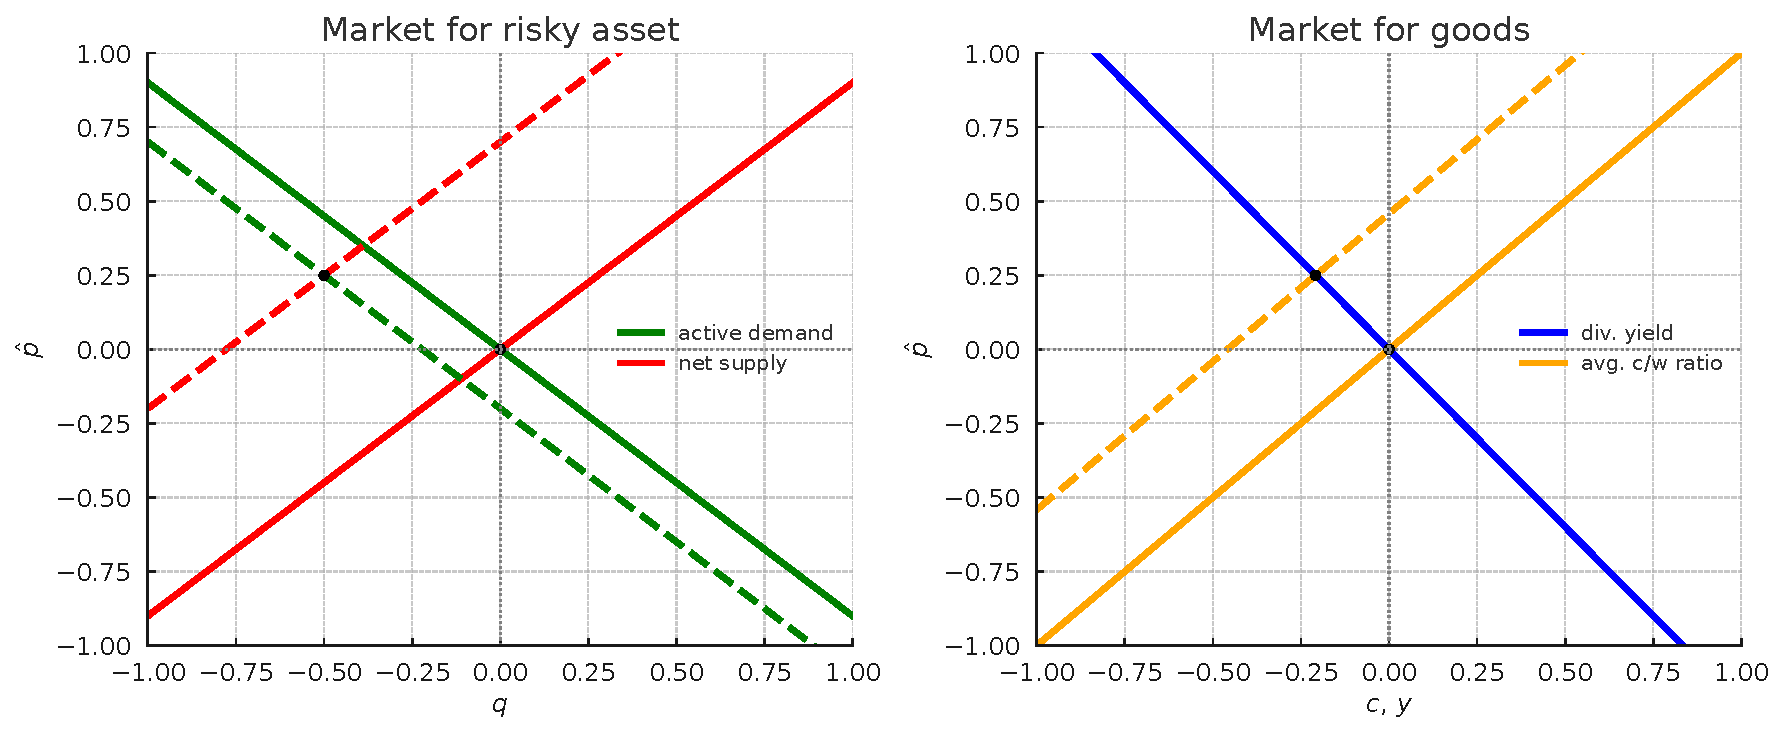
\includegraphics[width=0.95\linewidth]{figures/mkt_equilibrium2.pdf}
%     \caption{Equilibrium with inefficient risk allocation: risky-asset (left) and goods (right) markets.}
%     \label{fig:mkt_equilibrium2}
% \end{figure}


% Figure~\ref{fig:mkt_equilibrium2} illustrates the effects of portfolio flows when risk is initially concentrated on active investors, i.e., $\overline{\alpha}_{p,t}<1$. An inflow into the risky asset shifts the average consumption–wealth ratio curve leftward (right panel) and the net-supply curve leftward (left panel). The interest rate then adjusts so that active demand meets net supply at the goods-clearing price. In this case, portfolio flows have a positive price impact—the aggregate market elasticity is \emph{finite}.

% \begin{prop}[Aggregate elasticity: inefficient passive demand]\label{prop:elasticity_passive_demand}
%     % Suppose $\rho>\left(1-\psi^{-1}\right)\left( \mu - \frac{\gamma\|\sigma\|^2}{2}  \right)$. 
%     Without preference heterogeneity and leverage constraints, the inverse aggregate market elasticity $ \varepsilon^{-1}_{M,t} $ is
%     \begin{equation}\label{eq:elasticity_passive_demand}
%         \varepsilon_{M,t}^{-1}
%         \;=\;
%         -\,(\chi_{p}+y^*)^{-1}\,\frac{\partial \chi_{0,t}}{\partial f_t}
%         \;=\;
%         \left(1-\psi^{-1}\right)\frac{\gamma \|\sigma\|^{2}}{y^*}
%         \frac{1-\overline{\alpha}_{p,t}}{x_{a,t}}
%         \;+\;\mathcal{O}\!\left(\epsilon^{2}\right),
%     \end{equation}
%     where $x_{a,t}\equiv 1-x_{0,t}$ is the wealth share of active investors and $y^*\equiv 1/p^*$.
% \end{prop}

% Proposition~\ref{prop:elasticity_passive_demand} highlights the determinants of aggregate market elasticity. In contrast to \citet{gabaix2020search}, the risky-asset price elasticity $\zeta_p$—and the cross-elasticity $\zeta_r$—do not directly affect the aggregate elasticity. Given the recursive property of the demand system (where $r_t$ enters only the risky-asset demand), the price impact is determined by the properties of the consumption–wealth ratio.

% The market elasticity is finite whenever $\overline{\alpha}_{p,t}\neq 1$ and $\psi\neq 1$. In the unit-EIS case, the price–dividend ratio is pinned down by the subjective discount rate, so portfolio flows generate offsetting movements in the risk premium and the risk-free rate. When $\overline{\alpha}_{p,t}=1$, the risk allocation is initially efficient and, again, there is no price impact.

% The price impact is positive when $\psi>1$ and $\overline{\alpha}_{p,t}<1$: interest-rate adjustments no longer fully offset the response of the risk premium, so the risk-premium effect dominates. This parallels representative-agent models where uncertainty shocks require $\psi>1$ for the risk-premium channel to dominate \citep[e.g.,][]{bansal2004risks}.

% The state-global perturbation approach also shows that aggregate elasticity is \emph{state dependent}. 
% Figure~\ref{Fig:elasticity_passive-demand} plots the price impact as a function of active investors' wealth for different passive-share levels: it is larger when active investors are under-capitalized, highlighting the role of their risk-bearing capacity. 
% Price impact also increases with the distance of the passive share from its optimal value.
% For instance, when passive investors do not participate in equities ($\overline{\alpha}_{p,t}=0$), we recover a version of \citet{basak1998equilibrium} in which price impact is maximized.

% \begin{figure}[!t]
%     \centering
%     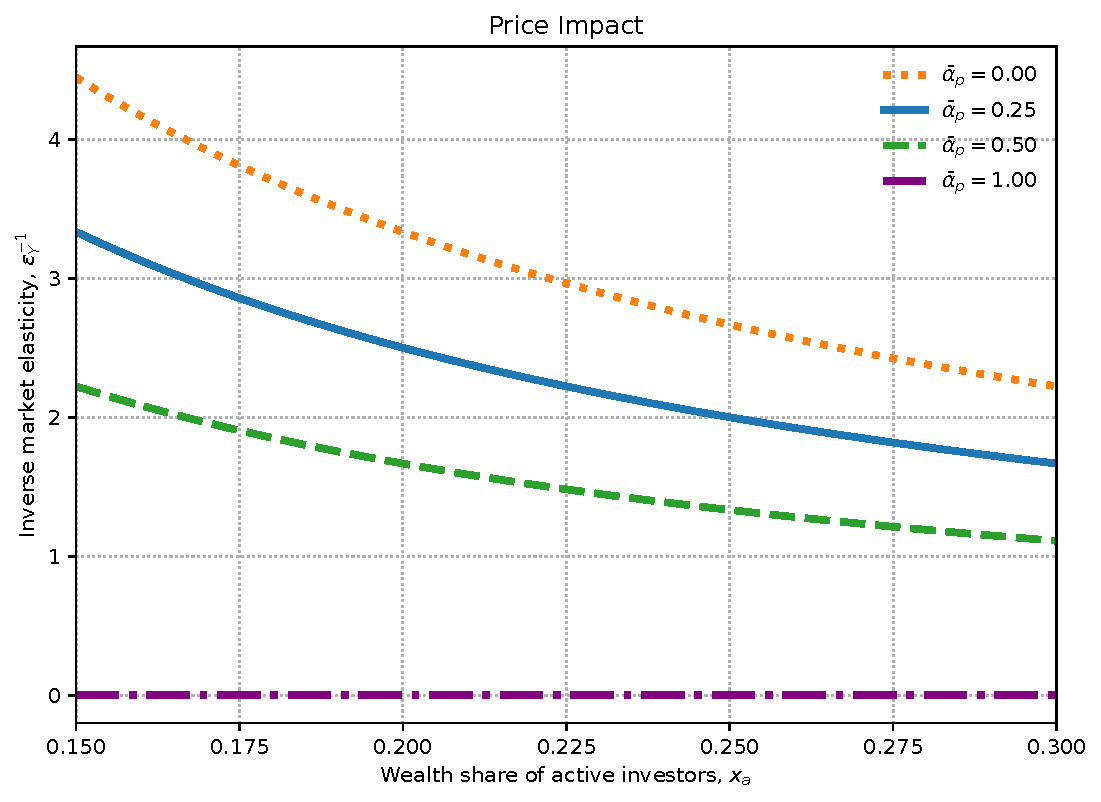
\includegraphics[width=0.65\textwidth]{./figures/price_impact_passive2.pdf}
%     \caption{Price impact: inefficient passive demand.}
%     \label{Fig:elasticity_passive-demand}
% \end{figure}

\subsection{Inefficient passive demand}

We next turn to a second-order approximation of the demand system to study how risk allocation affects aggregate market elasticity. To focus on the mechanism most clearly, consider the special case without preference heterogeneity or leverage constraints.  

\paragraph{The role of risk misallocation.}  
In this setting, demand for the risky asset is still given by \eqref{eq:demand_risky} up to second order. Without heterogeneity, the relevant demand shifter is  
\[
    f_t \equiv x_{0,t}\left(\overline{\alpha}_{p,t}-1\right),
\]
where $x_{0,t}$ denotes the wealth share of passive investors.  

The key difference relative to the benchmark arises from the consumption-wealth ratio. Aggregating \eqref{eq:xi_j} across investors, letting $c_t \equiv \sum_{j=0}^J x_{j,t} c_{j,t}$, and imposing market clearing $\sum_{j=0}^J x_{j,t}\alpha_{j,t}=1$, yields
\begin{equation}
    c_t
    \;=\;
    \psi\rho
    \;+\;
    (1-\psi)\!\left[
        r_t+\pi_t
        - \frac{\gamma\|\sigma\|^2}{2}\sum_{j=0}^J x_{j,t}\alpha_{j,t}^2
    \right]
    \;+\; \mathcal{O}(\epsilon^3).
\end{equation}
Under the efficient allocation $\alpha_{j,t}=1$, so $\sum_{j} x_{j,t}\alpha_{j,t}^2 = 1$. 
Any deviation from this efficient allocation creates dispersion in portfolios, leading to $\sum_j x_{j,t}\alpha_{j,t}^2>1$ by Jensen’s inequality, which lowers the risk-adjusted expected return $r_t+\pi_t - \tfrac{\gamma\|\sigma\|^2}{2}\sum_j x_{j,t}\alpha_{j,t}^2$. When $\psi>1$, this reduction weakens incentives to save and raises the consumption-wealth ratio for a given $r_t+\pi_t$.  

Movements in the passive portfolio therefore shift the aggregate consumption–wealth ratio. Its second-order expansion is
\begin{equation}
    \hat c_t \;\equiv\; c_t - c^*
    \;=\; \chi_{0,t} \;+\; \chi_p\,\hat p_t \;+\; \mathcal{O}(\epsilon^3),
\end{equation}
with coefficients
\[
    \chi_p = (\psi-1)\,\frac{1}{p^*},
    \qquad
    \chi_{0,t} = (\psi-1)\,\frac{\gamma\|\sigma\|^2}{2}\,
                    \frac{f_t^2}{x_{0,t}(1-x_{0,t})}.
\]
Because $\chi_{0,t}$ is quadratic in the flow $f_t$, it is $\mathcal{O}(\epsilon^2)$. For example, when passive investors are initially underexposed to the risky asset ($\overline{\alpha}_{p,t}<1$ and $\psi>1$), an inflow into stocks reduces the consumption-wealth ratio:
\[
    \frac{\partial \chi_{0,t}}{\partial f_t}
    \;=\;
    -\,(\psi-1)\,\gamma\|\sigma\|^2\,\frac{1-\overline{\alpha}_{p,t}}{1-x_{0,t}}.
\]
Note that $\chi_{0,t}$ is locally insensitive to portfolio flow changes when passive portfolio is efficient ($\overline{\alpha}_{p,t}=1$), consistent with the first-order analysis.  

\begin{figure}[t!]
    \centering
    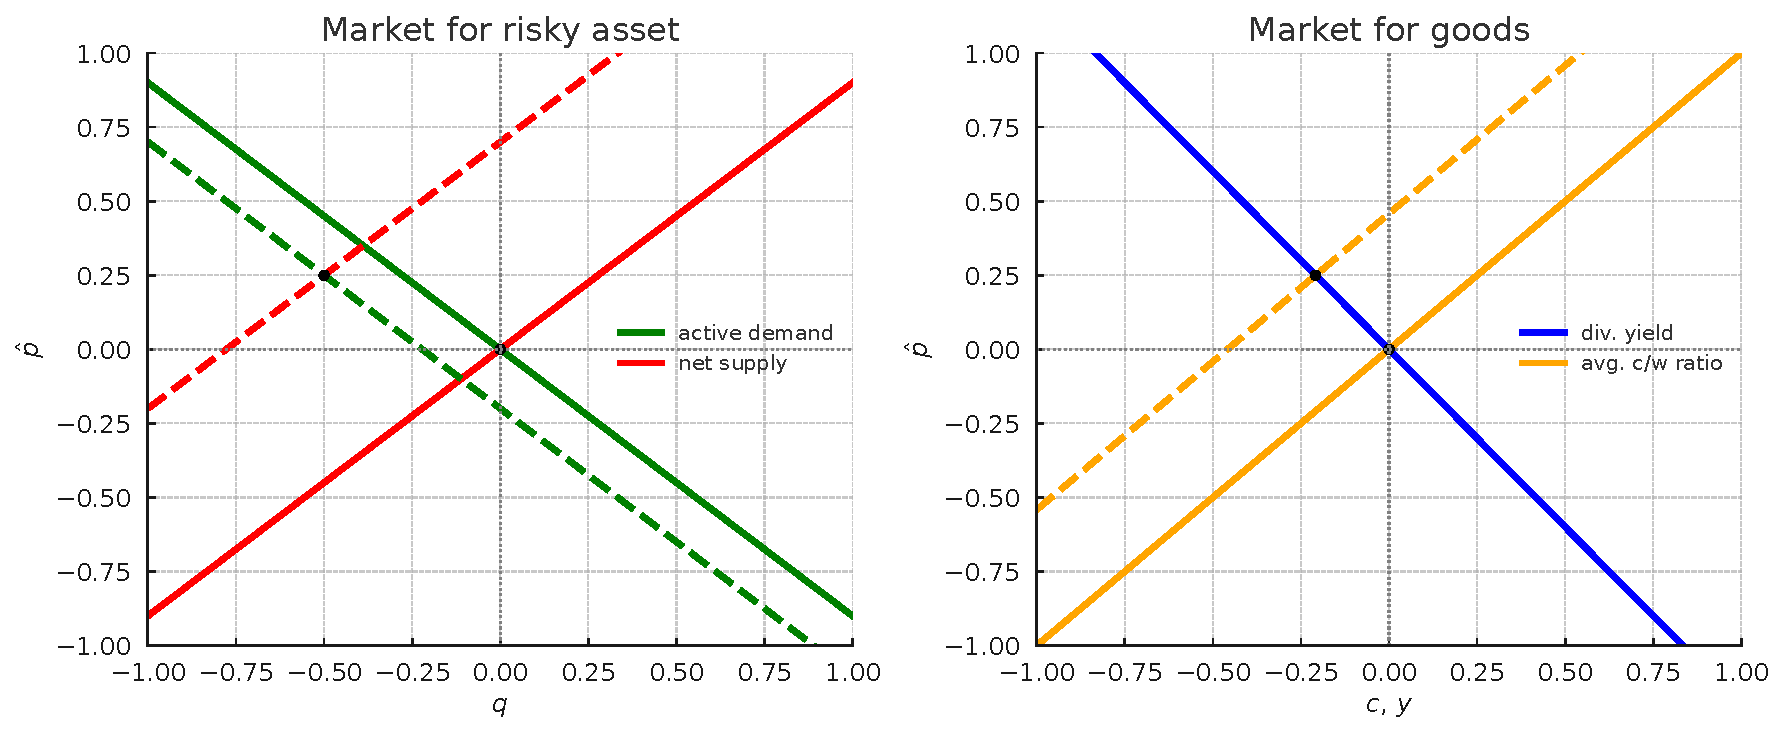
\includegraphics[width=0.95\linewidth]{figures/mkt_equilibrium2.pdf}
    \vspace{2mm}
    \caption{Equilibrium with inefficient risk allocation: risky asset (left) and goods (right) markets.}
    \label{fig:mkt_equilibrium2}
\end{figure}

Figure~\ref{fig:mkt_equilibrium2} illustrates the effects of portfolio flows when passive investors are initially underexposed to risk, i.e., $\overline{\alpha}_{p,t}<1$. An inflow into the risky asset shifts both the net supply curve (left panel) and the average consumption-wealth ratio schedule (right panel) leftward. The interest rate adjusts so that active demand meets net supply at the goods market clearing price. In this case, portfolio flows have a positive price impact and the aggregate elasticity is \textit{finite}.  

\begin{prop}[Aggregate elasticity: inefficient passive demand]\label{prop:elasticity_passive_demand}
Without preference heterogeneity or leverage constraints, the inverse aggregate elasticity is
\begin{equation}\label{eq:elasticity_passive_demand}
    \varepsilon_{M,t}^{-1}
    \;=\;
    -\,(\chi_{p}+y^*)^{-1}\,\frac{\partial \chi_{0,t}}{\partial f_t}
    \;=\;
    \left(1-\psi^{-1}\right)\frac{\gamma \|\sigma\|^{2}}{y^*}
    \frac{1-\overline{\alpha}_{p,t}}{x_{a,t}}
    \;+\;\mathcal{O}\!\left(\epsilon^{2}\right),
\end{equation}
where $x_{a,t}=1-x_{0,t}$ is the wealth share of active investors and $y^*=1/p^*$ is the dividend-price ratio in the benchmark economy.
\end{prop}

Proposition~\ref{prop:elasticity_passive_demand} shows that, unlike in \citet{gabaix2020search}, the risky-asset elasticities $\zeta_p$ and $\zeta_r$ are not the direct drivers of aggregate elasticity. Because the demand system is recursive (interest rates only enters the risky asset demand) the overall price impact is governed instead by how portfolio flows impact the consumption-wealth ratio. %In other words, aggregate elasticity reflects changes in savings behavior rather than the direct slope of risky asset demand.


The macro elasticity is finite whenever $\overline{\alpha}_{p,t}\neq 1$ and $\psi\neq 1$. In the unit EIS case, the price-dividend ratio is pinned down by the subjective discount rate, so portfolio flows generate offsetting movements in the risk premium and the risk-free rate. With efficient risk allocation ($\overline{\alpha}_{p,t}=1$), there is again no price impact.  

The price impact is positive when $\psi>1$ and $\overline{\alpha}_{p,t}<1$: interest rate adjustments no longer fully offset the risk premium response, so the latter dominates. This mirrors representative agent models in which uncertainty shocks affect prices only when $\psi>1$ \citep[e.g.,][]{bansal2004risks}.  

The state-global perturbation analysis also makes clear that elasticity is state dependent. Figure~\ref{Fig:elasticity_passive-demand} plots the price impact as a function of active investors' wealth for different passive-share levels.  Price impact rises when active investors are under capitalized, reflecting their limited risk-bearing capacity, and when the passive share deviates further from its efficient level. In the extreme case where passive investors hold no equities ($\overline{\alpha}_{p,t}=0$), we recover a version of \citet{basak1998equilibrium} in which price impact is maximized.  


\begin{figure}[!t]
    \centering
    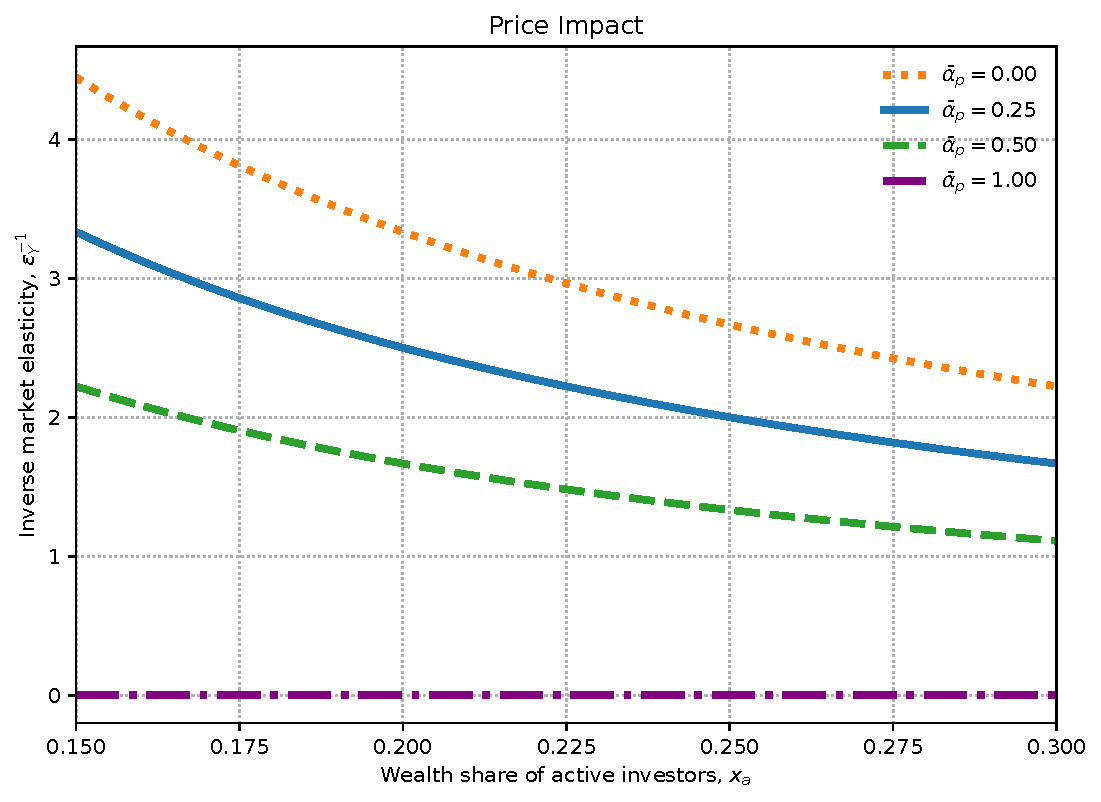
\includegraphics[width=0.65\textwidth]{./figures/price_impact_passive2.pdf}
    \vspace{2mm}
    \caption{Price impact: inefficient passive demand.}
    \label{Fig:elasticity_passive-demand}
\end{figure}



% In the absence of heterogeneity and leverage constraints, the demand for the risky asset under a second-order approximation takes the form in Equation \eqref{eq:demand_risky}, as shown in the appendix. In contrast, the consumption-wealth ratio is now given by
% \begin{equation}
%     c_{j,t} = \psi \rho + (1-\psi) \left[ r_t + \pi_t \alpha_{j,t} - \frac{\gamma \sigma^2}{2} \alpha_{j,t}^2 \right] + \xi_{j,t} + \mathcal{O}(\epsilon^3),
% \end{equation}
% where $\alpha_{0,t} = \overline{\alpha}_p $ and $\alpha_{j,t} = \frac{1-x_{0,t} \overline{\alpha}_p}{1-x_{0,t}}$ for $j = 1,\ldots, J$. Aggregating across investors, and using the market clearing condition $\sum_{j=0}^J x_j \alpha_{j,t} = 1$, we obtain
% \begin{equation}
%     c_t = \psi \rho + (1-\psi) \left[ r_t + \pi_t - \frac{\gamma \sigma^2}{2} \sum_{j=0}^J x_j \alpha_{j,t}^2 \right] + \mathcal{O}(\epsilon^3).
% \end{equation}

% The average consumption-wealth ratio now depends on the distribution of the risky asset in the economy. 
% Under the optimal allocation, the portfolio share is equal to one, $\alpha_{j,t} =1 $, for all investors, so $\sum_{j=0}^J x_j \alpha_{j,t}^2 = 1$. Any deviation of the optimal allocation creates dispersion in portfolios, so 
% $\sum_{j=0}^J x_j \alpha_{j,t}^2 > 1$, which reduces the risk-adjusted expected return $r_t + \pi_t - \frac{\gamma \sigma^2}{2} \sum_{j=0}^J x_j \alpha_{j,t}^2$. 
% If $\psi > 1$, the reduction in risk-adjusted returns weakens investors incentive to save, for any given level of $r_t +\pi_t$. 
% Therefore, the consumption-wealth ratio depends on how risk is allocated in the economy. 



% \begin{figure}[t!]
%     \centering

% \tikzset{every picture/.style={line width=0.75pt}} %set default line width to 0.75pt        

% \begin{tikzpicture}[x=0.75pt,y=0.75pt,yscale=-1,xscale=1]
% %uncomment if require: \path (0,235); %set diagram left start at 0, and has height of 235

% %Shape: Axis 2D [id:dp8667675453427319] 
% \draw [color={rgb, 255:red, 0; green, 0; blue, 0 }  ,draw opacity=1 ][line width=1.5]  (50,200) -- (289,200)(70,39) -- (70,222) (282,195) -- (289,200) -- (282,205) (65,46) -- (70,39) -- (75,46) (101,195) -- (101,205)(132,195) -- (132,205)(163,195) -- (163,205)(194,195) -- (194,205)(225,195) -- (225,205)(256,195) -- (256,205)(65,169) -- (75,169)(65,138) -- (75,138)(65,107) -- (75,107)(65,76) -- (75,76) ;
% \draw   ;
% %Shape: Arc [id:dp531658316023164] 
% \draw  [draw opacity=0][line width=2.25]  (69.96,200.56) .. controls (71.64,129.28) and (117.82,72.55) .. (173.1,73.85) .. controls (226.88,75.12) and (269.47,130.84) .. (270.19,199.49) -- (170.06,202.92) -- cycle ; \draw  [color={rgb, 255:red, 208; green, 2; blue, 27 }  ,draw opacity=1 ][line width=2.25]  (69.96,200.56) .. controls (71.64,129.28) and (117.82,72.55) .. (173.1,73.85) .. controls (226.88,75.12) and (269.47,130.84) .. (270.19,199.49) ;  
% %Shape: Circle [id:dp05697314227899386] 
% \draw  [draw opacity=0][fill={rgb, 255:red, 248; green, 231; blue, 28 }  ,fill opacity=0.5 ] (141.33,77.67) .. controls (141.33,74.17) and (144.17,71.33) .. (147.67,71.33) .. controls (151.16,71.33) and (154,74.17) .. (154,77.67) .. controls (154,81.16) and (151.16,84) .. (147.67,84) .. controls (144.17,84) and (141.33,81.16) .. (141.33,77.67) -- cycle ;
% %Shape: Circle [id:dp7553623057031522] 
% \draw  [draw opacity=0][fill={rgb, 255:red, 139; green, 87; blue, 42 }  ,fill opacity=0.5 ] (187.33,77.67) .. controls (187.33,74.17) and (190.17,71.33) .. (193.67,71.33) .. controls (197.16,71.33) and (200,74.17) .. (200,77.67) .. controls (200,81.16) and (197.16,84) .. (193.67,84) .. controls (190.17,84) and (187.33,81.16) .. (187.33,77.67) -- cycle ;
% %Shape: Axis 2D [id:dp8452210536537006] 
% \draw [color={rgb, 255:red, 0; green, 0; blue, 0 }  ,draw opacity=1 ][line width=1.5]  (377,199) -- (616,199)(397,38) -- (397,221) (609,194) -- (616,199) -- (609,204) (392,45) -- (397,38) -- (402,45) (428,194) -- (428,204)(459,194) -- (459,204)(490,194) -- (490,204)(521,194) -- (521,204)(552,194) -- (552,204)(583,194) -- (583,204)(392,168) -- (402,168)(392,137) -- (402,137)(392,106) -- (402,106)(392,75) -- (402,75) ;
% \draw   ;
% %Straight Lines [id:da8694501852937826] 
% \draw [color={rgb, 255:red, 245; green, 166; blue, 35 }  ,draw opacity=1 ][line width=1.5]    (347,55) -- (631,217) ;
% %Straight Lines [id:da4872089001830353] 
% \draw [color={rgb, 255:red, 74; green, 144; blue, 226 }  ,draw opacity=1 ][line width=1.5]    (343,199) -- (603,50) ;
% %Shape: Circle [id:dp6153612433225819] 
% \draw  [draw opacity=0][fill={rgb, 255:red, 139; green, 87; blue, 42 }  ,fill opacity=1 ] (222.33,97.67) .. controls (222.33,94.17) and (225.17,91.33) .. (228.67,91.33) .. controls (232.16,91.33) and (235,94.17) .. (235,97.67) .. controls (235,101.16) and (232.16,104) .. (228.67,104) .. controls (225.17,104) and (222.33,101.16) .. (222.33,97.67) -- cycle ;
% %Shape: Circle [id:dp4728310817061825] 
% \draw  [draw opacity=0][fill={rgb, 255:red, 248; green, 231; blue, 28 }  ,fill opacity=1 ] (107.33,97.67) .. controls (107.33,94.17) and (110.17,91.33) .. (113.67,91.33) .. controls (117.16,91.33) and (120,94.17) .. (120,97.67) .. controls (120,101.16) and (117.16,104) .. (113.67,104) .. controls (110.17,104) and (107.33,101.16) .. (107.33,97.67) -- cycle ;
% %Straight Lines [id:da6317730272289139] 
% \draw [color={rgb, 255:red, 0; green, 0; blue, 0 }  ,draw opacity=0.5 ][fill={rgb, 255:red, 0; green, 0; blue, 0 }  ,fill opacity=0 ]   (194,77.67) -- (226.93,96.67) ;
% \draw [shift={(228.67,97.67)}, rotate = 209.98] [color={rgb, 255:red, 0; green, 0; blue, 0 }  ,draw opacity=0.5 ][line width=0.75]    (10.93,-3.29) .. controls (6.95,-1.4) and (3.31,-0.3) .. (0,0) .. controls (3.31,0.3) and (6.95,1.4) .. (10.93,3.29)   ;
% %Straight Lines [id:da22117887446043505] 
% \draw [color={rgb, 255:red, 0; green, 0; blue, 0 }  ,draw opacity=0.5 ][fill={rgb, 255:red, 0; green, 0; blue, 0 }  ,fill opacity=0 ]   (147.67,77.67) -- (115.39,96.65) ;
% \draw [shift={(113.67,97.67)}, rotate = 329.53] [color={rgb, 255:red, 0; green, 0; blue, 0 }  ,draw opacity=0.5 ][line width=0.75]    (10.93,-3.29) .. controls (6.95,-1.4) and (3.31,-0.3) .. (0,0) .. controls (3.31,0.3) and (6.95,1.4) .. (10.93,3.29)   ;
% %Straight Lines [id:da6847983852102553] 
% \draw [color={rgb, 255:red, 74; green, 144; blue, 226 }  ,draw opacity=1 ][line width=1.5]  [dash pattern={on 1.69pt off 2.76pt}]  (348,206) -- (608,57) ;

% % Text Node
% \draw (284,214) node  [color={rgb, 255:red, 0; green, 0; blue, 0 }  ,opacity=1 ,rotate=-358.98]  {$port.\ share$};
% % Text Node
% \draw (42,39) node  [color={rgb, 255:red, 0; green, 0; blue, 0 }  ,opacity=1 ,rotate=-358.98]  {$return$};
% % Text Node
% \draw (74,10.43) node [anchor=north west][inner sep=0.75pt]   [align=left] {\textbf{Risk-adjusted excess return}};
% % Text Node
% \draw (544,67) node  [color={rgb, 255:red, 74; green, 144; blue, 226 }  ,opacity=1 ,rotate=-329.57]  {$avg.\ c/w\ ratio$};
% % Text Node
% \draw (639,200) node  [color={rgb, 255:red, 0; green, 0; blue, 0 }  ,opacity=1 ,rotate=-358.98]  {$c,y$};
% % Text Node
% \draw (578,170) node  [color={rgb, 255:red, 245; green, 166; blue, 35 }  ,opacity=1 ,rotate=-28.61]  {$div.\ yield$};
% % Text Node
% \draw (381,38) node  [color={rgb, 255:red, 0; green, 0; blue, 0 }  ,opacity=1 ,rotate=-358.98]  {$p$};
% % Text Node
% \draw (434,3.43) node [anchor=north west][inner sep=0.75pt]   [align=left] {\textbf{Market for goods}};
% % Text Node
% \draw (239,89) node [anchor=north west][inner sep=0.75pt]   [align=left] {\textbf{a}};
% % Text Node
% \draw (95,87) node [anchor=north west][inner sep=0.75pt]   [align=left] {\textbf{p}};


% \end{tikzpicture}    
% \caption{Consumption-wealth ratio when risk is nearly perfectly allocated}    \label{fig:mkt_equilibrium_misallocation}
% \end{figure}

% Figure~\ref{fig:mkt_equilibrium_misallocation2} illustrates how an increase in risk misallocation affects the equilibrium in the goods market. 
% The left panel represents the risk-adjusted excess return, $\pi_t \alpha_{j,t} - \frac{\gamma \sigma^2}{2} \alpha_{j,t}^2$, as a function of the portfolio share $\alpha_{j,t}$. 
% Suppose that the passive investor has initially a portfolio share that is less than one and then decides to further reduce its holding of the risky asset, as represented by the yellow dot in the figure. 
% Even if the risk premium is constant, the risk-adjusted return is reduced, as the investor moves  away from the optimal holding of the risky asset. 
% The portfolio share of the active investors also moves away from the optimal, as represented by the brown dot in the figure, so the risk-adjusted return is reduced for them as well. 
% Therefore, both agents have a weaker incentive to save, which leads to a shift in the average consumption-wealth ratio, as shown in the right panel. 

% \begin{figure}[t!]
%     \centering

%     \begin{tikzpicture}[x=0.75pt,y=0.75pt,yscale=-1,xscale=1]
% %uncomment if require: \path (0,235); %set diagram left start at 0, and has height of 235

% %Shape: Axis 2D [id:dp17811910341215076] 
% \draw [color={rgb, 255:red, 0; green, 0; blue, 0 }  ,draw opacity=1 ][line width=1.5]  (50,200) -- (289,200)(70,39) -- (70,222) (282,195) -- (289,200) -- (282,205) (65,46) -- (70,39) -- (75,46) (101,195) -- (101,205)(132,195) -- (132,205)(163,195) -- (163,205)(194,195) -- (194,205)(225,195) -- (225,205)(256,195) -- (256,205)(65,169) -- (75,169)(65,138) -- (75,138)(65,107) -- (75,107)(65,76) -- (75,76) ;
% \draw   ;
% %Shape: Arc [id:dp2728896334946356] 
% \draw  [draw opacity=0][line width=2.25]  (69.96,200.56) .. controls (71.64,129.28) and (117.82,72.55) .. (173.1,73.85) .. controls (226.88,75.12) and (269.47,130.84) .. (270.19,199.49) -- (170.06,202.92) -- cycle ; \draw  [color={rgb, 255:red, 208; green, 2; blue, 27 }  ,draw opacity=1 ][line width=2.25]  (69.96,200.56) .. controls (71.64,129.28) and (117.82,72.55) .. (173.1,73.85) .. controls (226.88,75.12) and (269.47,130.84) .. (270.19,199.49) ;  
% %Shape: Circle [id:dp09152732788574003] 
% \draw  [draw opacity=0][fill={rgb, 255:red, 248; green, 231; blue, 28 }  ,fill opacity=0.5 ] (105.33,100.67) .. controls (105.33,97.17) and (108.17,94.33) .. (111.67,94.33) .. controls (115.16,94.33) and (118,97.17) .. (118,100.67) .. controls (118,104.16) and (115.16,107) .. (111.67,107) .. controls (108.17,107) and (105.33,104.16) .. (105.33,100.67) -- cycle ;
% %Shape: Circle [id:dp8702384042700901] 
% \draw  [draw opacity=0][fill={rgb, 255:red, 139; green, 87; blue, 42 }  ,fill opacity=0.5 ] (224.33,100.67) .. controls (224.33,97.17) and (227.17,94.33) .. (230.67,94.33) .. controls (234.16,94.33) and (237,97.17) .. (237,100.67) .. controls (237,104.16) and (234.16,107) .. (230.67,107) .. controls (227.17,107) and (224.33,104.16) .. (224.33,100.67) -- cycle ;
% %Shape: Axis 2D [id:dp6014255008545599] 
% \draw [color={rgb, 255:red, 0; green, 0; blue, 0 }  ,draw opacity=1 ][line width=1.5]  (377,199) -- (616,199)(397,38) -- (397,221) (609,194) -- (616,199) -- (609,204) (392,45) -- (397,38) -- (402,45) (428,194) -- (428,204)(459,194) -- (459,204)(490,194) -- (490,204)(521,194) -- (521,204)(552,194) -- (552,204)(583,194) -- (583,204)(392,168) -- (402,168)(392,137) -- (402,137)(392,106) -- (402,106)(392,75) -- (402,75) ;
% \draw   ;
% %Straight Lines [id:da943055555850097] 
% \draw [color={rgb, 255:red, 245; green, 166; blue, 35 }  ,draw opacity=1 ][line width=1.5]    (347,55) -- (631,217) ;
% %Straight Lines [id:da12202983705810633] 
% \draw [color={rgb, 255:red, 74; green, 144; blue, 226 }  ,draw opacity=1 ][line width=1.5]    (343,199) -- (603,50) ;
% %Shape: Circle [id:dp9185533411503766] 
% \draw  [draw opacity=0][fill={rgb, 255:red, 139; green, 87; blue, 42 }  ,fill opacity=1 ] (259.33,160.67) .. controls (259.33,157.17) and (262.17,154.33) .. (265.67,154.33) .. controls (269.16,154.33) and (272,157.17) .. (272,160.67) .. controls (272,164.16) and (269.16,167) .. (265.67,167) .. controls (262.17,167) and (259.33,164.16) .. (259.33,160.67) -- cycle ;
% %Shape: Circle [id:dp458319980377794] 
% \draw  [draw opacity=0][fill={rgb, 255:red, 248; green, 231; blue, 28 }  ,fill opacity=1 ] (71.33,159.67) .. controls (71.33,156.17) and (74.17,153.33) .. (77.67,153.33) .. controls (81.16,153.33) and (84,156.17) .. (84,159.67) .. controls (84,163.16) and (81.16,166) .. (77.67,166) .. controls (74.17,166) and (71.33,163.16) .. (71.33,159.67) -- cycle ;
% %Straight Lines [id:da5461592683560248] 
% \draw [color={rgb, 255:red, 0; green, 0; blue, 0 }  ,draw opacity=0.5 ][fill={rgb, 255:red, 0; green, 0; blue, 0 }  ,fill opacity=0 ]   (230.67,100.67) -- (264.66,158.94) ;
% \draw [shift={(265.67,160.67)}, rotate = 239.74] [color={rgb, 255:red, 0; green, 0; blue, 0 }  ,draw opacity=0.5 ][line width=0.75]    (10.93,-3.29) .. controls (6.95,-1.4) and (3.31,-0.3) .. (0,0) .. controls (3.31,0.3) and (6.95,1.4) .. (10.93,3.29)   ;
% %Straight Lines [id:da04864508639252052] 
% \draw [color={rgb, 255:red, 0; green, 0; blue, 0 }  ,draw opacity=0.5 ][fill={rgb, 255:red, 0; green, 0; blue, 0 }  ,fill opacity=0 ]   (111.67,100.67) -- (78.67,157.93) ;
% \draw [shift={(77.67,159.67)}, rotate = 299.95] [color={rgb, 255:red, 0; green, 0; blue, 0 }  ,draw opacity=0.5 ][line width=0.75]    (10.93,-3.29) .. controls (6.95,-1.4) and (3.31,-0.3) .. (0,0) .. controls (3.31,0.3) and (6.95,1.4) .. (10.93,3.29)   ;
% %Straight Lines [id:da7145890387073353] 
% \draw [color={rgb, 255:red, 74; green, 144; blue, 226 }  ,draw opacity=1 ][line width=1.5]  [dash pattern={on 1.69pt off 2.76pt}]  (372,232) -- (632,83) ;

% % Text Node
% \draw (284,214) node  [color={rgb, 255:red, 0; green, 0; blue, 0 }  ,opacity=1 ,rotate=-358.98]  {$port.\ share$};
% % Text Node
% \draw (42,39) node  [color={rgb, 255:red, 0; green, 0; blue, 0 }  ,opacity=1 ,rotate=-358.98]  {$return$};
% % Text Node
% \draw (74,10.43) node [anchor=north west][inner sep=0.75pt]   [align=left] {\textbf{Risk-adjusted excess return}};
% % Text Node
% \draw (544,67) node  [color={rgb, 255:red, 74; green, 144; blue, 226 }  ,opacity=1 ,rotate=-329.57]  {$avg.\ c/w\ ratio$};
% % Text Node
% \draw (639,200) node  [color={rgb, 255:red, 0; green, 0; blue, 0 }  ,opacity=1 ,rotate=-358.98]  {$c,y$};
% % Text Node
% \draw (578,170) node  [color={rgb, 255:red, 245; green, 166; blue, 35 }  ,opacity=1 ,rotate=-28.61]  {$div.\ yield$};
% % Text Node
% \draw (381,38) node  [color={rgb, 255:red, 0; green, 0; blue, 0 }  ,opacity=1 ,rotate=-358.98]  {$p$};
% % Text Node
% \draw (434,3.43) node [anchor=north west][inner sep=0.75pt]   [align=left] {\textbf{Market for goods}};
% % Text Node
% \draw (247,152) node [anchor=north west][inner sep=0.75pt]   [align=left] {\textbf{a}};
% % Text Node
% \draw (90,151) node [anchor=north west][inner sep=0.75pt]   [align=left] {\textbf{p}};


% \end{tikzpicture}
%          \caption{Consumption-wealth ratio when risk is highly misallocated}
%     \label{fig:mkt_equilibrium_misallocation2}
% \end{figure}

% The magnitude of the shift in the average consumption-wealth ratio depends on the initial distribution of risk. 
% This point can be seen more clearly by writing the average consumption-wealth in terms of deviations from its value in the benchmark economy:
% \begin{equation}
%     \hat{c}_{t} = \zeta_{p}^c \hat{p}_t + \zeta_{0}^c,
% \end{equation}
% where $\zeta_0^c = (\psi-1) \frac{\gamma \sigma^2}{2} \sum_{j=0}^J x_j (\alpha_{j,t}-1)^2$. Notice that $\zeta_0^c$ is a function of $\overline{\alpha}_p$ and the derivative of $\zeta_0^c$ with respect to $\overline{\alpha}_p$ is given by
% \begin{equation}
%     \left. \frac{\partial \zeta_0^c}{\partial \overline{\alpha}_p} \right|_{\overline{\alpha}_p = 1} =  \left.(\psi-1) \gamma \sigma^2 \sum_{j=0}^J x_j (\alpha_{j,t}-1) \frac{\partial \alpha_{j,t}}{\partial \overline{\alpha}_p}\right|_{\overline{\alpha}_p = 1} = 0.
% \end{equation}
% If the passive investor initially holds the optimal portfolio, then a small change in $\overline{\alpha}_p$ has no impact in the consumption-wealth ratio. 
% This corresponds to the frictionless benchmark, which is analogous to the result under the first-order approximation. 
% However, if the initial allocation of risk is not optimal, changes in $\overline{\alpha}_p$ affect the consumption-wealth ratio. 
% Moreover, the effect is stronger the further the initial allocation is from the optimal. 
% This point is illustrated in Figure~\ref{fig:mkt_equilibrium_misallocation2}.
% The initial allocation is now further away from the optimal relative to the case in Figure~\ref{fig:mkt_equilibrium_misallocation2}, which leads to a larger decline in the risk-adjusted returns, as shown in the left panel. 
% In this case, we see a larger shift in the average consumption-wealth curve in the right panel. 



% \paragraph{The market elasticity with inefficient passive demand.} The equilibrium value for asset prices takes the same shape as in the case of the first-order approximation:
% \begin{equation}
%     \hat{p}_t = - \frac{\zeta_0^c}{\zeta_p^c + \frac{1}{p^*} }, \qquad \qquad 
%     \hat{r}_t = \frac{f_t}{\zeta_r^q} + \frac{\zeta_p^q}{\zeta_r^q \left( \zeta_p^c + \frac{1}{p^*} \right)} \zeta_0^c.\nonumber
% \end{equation}
% As before, the price of the risky asset is independent of the (micro) price elasticity $\zeta_p^q$. However, while the shifter $\zeta_0^c$ was independent of $\overline{\alpha}_p$ under a first-order approximation, this is not the case now, as $\zeta_0^c$ is a function of $\overline{\alpha}_p$. The next proposition derives the aggregate market elasticity in this case.

% \begin{prop}[Aggregate elasticity: inefficient passive demand]\label{prop:elasticity_passive_demand2}
% 	Suppose $\rho>\left(1-\psi^{-1}\right)\left( \mu - \frac{\gamma\sigma^2}{2}  \right)$. 
% 	If there is no preference heterogeneity and active investors do not face leverage constraints, the inverse aggregate market elasticity, $ 1/\varepsilon_M $, is given by:
% 	\begin{equation}\label{eq:elasticity_passive_demand}
% %		\frac{1}{p(X, \epsilon)} \frac{\partial p(X, \epsilon)}{\partial F(X, \epsilon)}
% 		\varepsilon_M^{-1}=\left(1-\psi^{-1}\right) \frac{\gamma \sigma^{2}}{y_{0}(X)} \frac{1-\overline{\alpha}_{p}}{x_{a}}+\mathcal{O}\left(\epsilon^{2}\right),		
% 	\end{equation}		
% 	where $ x_{a} \equiv 1-x_{0} $ denotes the wealth share of active investors and $y_0(x) = 1/p_0(X)$.
% \end{prop}
% \begin{proof}
% 	See Appendix~\ref{app:prop_elasticity_passive_demand}.
% \end{proof}



% We highlight several points from Proposition~\ref{prop:elasticity_passive_demand}. First, the price impact is equal to zero if $\overline{\alpha}_p$, that is, the market is infinitely elastic when risk is initially optimally allocated. Second, the price impact is also zero if the EIS is equal to one. 
% In this case, the consumption-wealth ratio is constant and $\zeta_0^c = 0$, so $\overline{\alpha}_p$ does not affect investors' incentive to save.
% Third, the market elasticity is positive if $\psi > 1$ and $\overline{\alpha}_p < 1$, so passive investors hold an inefficiently low share of the risky asset. 
% This result is consistent with the discussion in Section~\ref{sec:simple}, which shows that we obtain a finite elasticity when movements in the passive portfolio share shifts not only the net supply of risk to active investors, but also the consumption-wealth ratio. 
% As discussed above, risk misallocation provides a mechanism linking changes in $\overline{\alpha}_p$ to shifts in the consumption-wealth ratio. 
% % Moreover, the price impact is increasing in the degree of misallocation, as an increase in $\overline{\alpha}_p$ raises the price of the risky asset by more when $\overline{\alpha}_p$ is further away from 1, the optimal portfolio share in this economy. 
% Moreover, everything else constant, the price impact is largest in the case of no market participation by passive investors $(\overline{\alpha}_{p,t} = 0)$, as in e.g. \citet{basak1998equilibrium}, given that this corresponds to the maximum level of misallocation (given $\overline{\alpha}_p\geq 0$).
% Fourth, the elasticity is state-dependent and the price impact is larger when active investors are under-capitalized, that is, they hold a relatively small share of wealth. 
% Figure~\ref{Fig:elasticity_passive-demand} illustrate these points. We can see that the price impact is equal to zero when $\overline{\alpha}_p = 1$, it is positive when $\overline{\alpha}_p < 1$, it is decreasing in wealth share of active investors $x_a$, and it is largest when $\overline{\alpha}_p = 0$ for any given level of $x_a$.


% In Proposition~\ref{prop:second_order} in Appendix~\ref{app:prop_second_order}, we consider the second-order correction.
%\begin{prop}[Second-order correction]\label{prop:second_order}
%	Suppose $\rho>\left(1-\psi^{-1}\right)\left( \mu - \frac{\gamma
%		\sigma^2}{2}  \right)$.  Then,
%	\begin{enumerate}[(i)]
%		\item The second-order correction for the consumption-wealth ratio and risk exposure are given by:
%		\begin{align}
%		\xi_{j,2}(X) &= (1-\psi) \frac{\gamma \sigma^2}{2} \left[ \left(1-\psi^{-1}\right) \sum_{k=0}^J x_{k,t} \hat{\gamma}_k -\hat{\gamma}_j \right]\nonumber\\
%		%		\sigma_{j,1}(X) &= \sigma\min\left\{ \sum_{k\in\mathcal{J}^u} \frac{x_k}{x_u} \hat{\gamma}_k- \hat{\gamma}_j  -\frac{\hat{\alpha}_p  x_0+\frac{\hat{\sigma}}{\sigma} x_c }{1-x_0-x_c},\frac{\hat{\sigma}}{\sigma}  \right\}.\nonumber
%		\sigma_{j,2}(X) &= \frac{\eta_2(X)}{\gamma} - \frac{\eta_1(X)}{\gamma}\hat{\gamma}_j + \frac{\eta_0(X)}{\gamma}\hat{\gamma}_j^2 - (1-\gamma^{-1})   \sigma_{y,2}(X),\nonumber
%		\end{align}
%		where 
%		\begin{equation*}
%		\sigma_{y,2}(X)  = \left(1-\psi^{-1}\right)\frac{\gamma\sigma^2}{2 y_{0}(X)} \sum_{k=1}^J \left( \hat{\gamma}_k - \hat{\gamma}_0  \right) x_k \sigma_{k,1}(X).
%		\end{equation*}
%		\item The second-order correction for the Sharpe ratio, interest rate, and dividend yield are given by:
%		\begin{align}		
%		\eta_2(X) &=  - \frac{(\gamma-1) x_c + 1-x_0}{1-x_0-x_c} \sigma_{y,2}(X) - \gamma \sigma \mathbb{E}^u[\hat{\gamma}_j] \frac{ \hat{\alpha}_p x_0+ \frac{\hat{\sigma}}{\sigma}x_c }{1-x_0-x_c} - \gamma \sigma \var^u[\hat{\gamma}_j]\nonumber	\\	
%		%		r_1(X) &=\gamma\sigma^2 \left[ -\sum_{j\in\mathcal{J}^u} \frac{x_j}{x_u} \hat{\gamma}_j +\left(1-\psi^{-1}\right) \sum_{j=0}^J x_{j,t}\frac{\hat{\gamma}_j}{2}+\frac{\hat{\alpha}_p  x_0+\frac{\hat{\sigma}}{\sigma} x_c }{1-x_0-x_c} \right]\nonumber\\
%		r_2(X) &= - \eta_2(X) \sigma + \eta_0(X) \sigma_{y,2}(X)-\psi^{-1} (\mu_{y,2}(X) + \sigma \sigma_{y,2}(X))\nonumber\\
%		&\quad+ \left(1-\psi^{-1}\right) \sum_{j=0}^J x_{j} \gamma\sigma \left[ \sigma_{j,2}(X) + \frac{\sigma_{j,1}^2(X)}{2 \sigma} + \hat{\gamma}_j \sigma_{j,1} \right]\nonumber\\
%		&\quad+\psi^{-1} \sum_{j=0}^J x_{j}\left[ \mu_{\xi_j,2}(X) + (1-\gamma) \sigma_{\xi_j,2}(X) \sigma \right]\nonumber\\
%		y_2(X) &= \left(1-\psi^{-1}\right)\left[\gamma \sigma_{y, 2}(X) \sigma+\sum_{j=0}^{J} x_{j} \gamma \sigma\left(\frac{\sigma_{j, 1}^{2}(X)}{2 \sigma}+\sigma_{j, 2}(X)+\hat{\gamma}_{j} \sigma_{j, 1}(X)\right)\right],\nonumber
%		\end{align}
%		where 
%		\[\mathbb{E}^{u}[\hat{\gamma}_{j}] \equiv \sum_{j \in \mathcal{J}^{u}} \frac{x_{j}}{x_{u}} \hat{\gamma}_{j}, \quad \text { and } \quad \var^{u}[\hat{\gamma}_{j}] \equiv \sum_{j \in \mathcal{J}^{u}} \frac{x_{j}}{x_{u}} \hat{\gamma}_{j}^{2}-\left(\sum_{j \in \mathcal{J}^{u}} \frac{x_{j}}{x_{u}} \hat{\gamma}_{j}\right)^{2}.\]
%	\end{enumerate}
%\end{prop}
%\begin{proof}
%	See Appendix~\ref{app:prop_second_order}. 
%\end{proof}
%\textcolor{red}{Need to discuss the intuition and why we need to have second-order correction. Perhaps this needs to be moved after we discuss that there is no price impact up to first order.}
% We can write the second-order expansion of the price-dividend ratio $p(X,\epsilon)$ as:
% \begin{equation}
% p(X,\epsilon) = \frac{1}{y_0(X)} - \frac{y_1(X)}{y_0^2(X)} \epsilon + \left[ \frac{y_1^2(X)}{y_0^3(X)} - \frac{y_{2}(X)}{y_0^2(X)} \right] \epsilon^2 + \mathcal{O}(\epsilon^3).
% \end{equation}

% Therefore, we can derive the inverse elasticity as:
% \begin{equation}\label{eq:elasticity-y2}
% \varepsilon_M^{-1}=\frac{1}{p(X,\epsilon)}\frac{\partial p(X,\epsilon)}{\partial F(X,\epsilon)} = - \frac{1}{y_0(X)} \frac{\partial y_2(X)}{\partial \hat{\alpha}_p}\frac{\epsilon}{x_0} + \mathcal{O}(\epsilon^2),
% \end{equation}
% where the second-order correction of the dividend yield $ y_2 $ is given in Proposition~\ref{prop:second_order}. 
% Note that from Proposition~\ref{prop:first_order}, $ y_1(X) $ does not depend on $ \hat{\alpha}_p $, leading to no price impact (infinite elasticity) up to the first-order.





% \subsection{Passive demand}
% In Proposition~\ref{prop:elasticity_passive_demand}, we consider the impact of passive demand on the aggregate elasticity by shutting down preference heterogeneity and portfolio constraints.
% \begin{prop}[Aggregate elasticity: passive demand]\label{prop:elasticity_passive_demand2}
% 	Suppose $\rho>\left(1-\psi^{-1}\right)\left( \mu - \frac{\gamma\sigma^2}{2}  \right)$. 
% 	If there is no preference heterogeneity and active investors do not face leverage constraints, the inverse aggregate market elasticity, $ 1/\varepsilon_M $, is given by:
% 	\begin{equation}\label{eq:elasticity_passive_demand}
% %		\frac{1}{p(X, \epsilon)} \frac{\partial p(X, \epsilon)}{\partial F(X, \epsilon)}
% 		\varepsilon_M^{-1}=\left(1-\psi^{-1}\right) \frac{\gamma \sigma^{2}}{y_{0}(X)} \frac{1-\overline{\alpha}_{p}}{x_{a}}+\mathcal{O}\left(\epsilon^{2}\right),		
% 	\end{equation}		
% 	where $ x_{a} \equiv 1-x_{0} $ denotes the wealth share of active investors.
% \end{prop}
% \begin{proof}
% 	See Appendix~\ref{app:prop_elasticity_passive_demand}.
% \end{proof}
% We highlight several points from Proposition~\ref{prop:elasticity_passive_demand}. 
% %\textcolor{red}{The first point probably needs to move.} First, given that in the absence of investor heterogeneity and leverage constraints the second-order correction for the Sharpe ratio is zero ($ \eta_2(X) =0$), the price impact of flows is entirely driven by its second-order impact on the risk-free rate, $ r_2(X) $. In particular, we have $ r_2(X)=y_2(X) $, and
% %\begin{align}
% %	\frac{\partial \pi(X,\epsilon)}{\partial F(X,\epsilon)} &= 	-\frac{\gamma \sigma^2}{x_u}  +\mathcal{O}(\epsilon^2),\label{eq:rp-passive-demand}\\
% %	\frac{\partial r(X,\epsilon)}{\partial F(X,\epsilon)} &= \frac{\gamma \sigma^2}{x_u} +\left(1-\psi^{-1}\right) \gamma \sigma^{2} \frac{1-\overline{\alpha}_{p}}{x_{a}}+\mathcal{O}(\epsilon^2)\label{eq:r-passive-demand},
% %\end{align}
% %where $ \pi_t $ is the risk premium on the risky asset defined above.
% First, the price impact is stronger the smaller the passive investors' portfolio share $ \overline{\alpha}_p $. This is shown in Figure~\ref{Fig:elasticity_passive-demand}. Consider the extreme case of no market participation by passive investors when $ \overline{\alpha}_p=0 $ (as in e.g., \citealp{basak1998equilibrium}). In this case, if we allow passive agents to permanently increase their risky asset holdings from 0 to $ W_0\hat{\alpha}_p\epsilon $, then with second-order correction, flows still have a price impact, leading to a finite market elasticity. %Again, with $ \psi>1 $, from Equation~\eqref{eq:elasticity_passive_demand}, we see an \textit{increase} in the price-dividend ratio as a result. 
% Notably, the market becomes more macro inelastic relative to the case in which there is passive demand and $ \overline{\alpha}_p>0 $. In other words, the more risk is concentrated in the hands of active investors, the more compensation they demand for holding the risky asset, and the more inelastic market becomes. %It's about quantity of risk reducing the misallocation of risk.
% %\textcolor{red}{Need to better explain the elasticity in the limited participation case.}

% \textbf{Compare with Koijen and Gabaix. How would we get a multiplier of 5 here?} 


% Second, with the second-order correction, if we start at the frictionless Lucas economy benchmark with $ \overline{\alpha}_p=1 $, we arrive at an infinite aggregate elasticity as before where flows have no impact on the price-dividend ratio. %This immediately follows from Equation~\eqref{eq:rp-passive-demand} and \eqref{eq:r-passive-demand}, as 
% In this case, the effect of portfolio flows on the risk premium and the risk-free rate exactly offset each other again.

% Next, the sign and magnitude of the aggregate market elasticity depends on the EIS, $ \psi $, reemphasizing the key role that GE effects play in our model. When passive investors sell bonds to invest in stocks, the risk premium and interest rate move in opposite directions. With $ \psi>1 $,  the risk premium goes down more, leading to an increase in the price-dividend ratio. 
% This is in contrast to Proposition~\ref{prop:elasticity_first_order} where these effects exactly cancel each other out leading to no price impact up to the first order.
% %\textcolor{red}{Perhaps also mention \cite{gabaix2020search} and their non-traditional GE/PE setting?}

% Finally, note that from Equation~\eqref{eq:elasticity_passive_demand}, the market elasticity is time-varying and state-dependent. In particular, as shown in Figure~\ref{Fig:elasticity_passive-demand}, when $ x_a $ is low and active investors are undercapitalized, there is a larger price response to flows and the market is more macro inelastic. 



% \subsection{Preference heterogeneity and leverage constraints}

% We now return to the model with preference heterogeneity and leverage constraints. 
% The next proposition provides the main result of this section.

% \begin{prop}[Aggregate elasticity: heterogeneity and leverage constraints]\label{prop_elasticity_pref_heterog}
%     The inverse aggregate market elasticity is
%     \begin{equation}\label{eq:elasticity_pref_heterog}
%         \varepsilon_{M,t}^{-1}
%         \;=\;
%         \bigl(1-\psi^{-1}\bigr)\,
%         \frac{\gamma\,\|\sigma\|^{2}}{y^*}\,
%         \frac{\overline{\alpha}_{p,t}^{\mathrm{opt}}-\overline{\alpha}_{p,t}}{x_{a,t}}\,
%         \bigl(1-x_{c,t}\bigr)
%         \;+\;\mathcal{O}\!\left(\epsilon^{2}\right),
%     \end{equation}
%     where \(x_{c,t}\) is the wealth share of \emph{constrained} active investors and the passive investors' optimal portfolio share is
%     \begin{equation}\label{eq:optimal_alpha_p}
%         \overline{\alpha}_{p,t}^{\mathrm{opt}}
%         \;=\;
%         1
%         \;-\;
%         \frac{x_{a,t}-x_{c,t}}{1-x_{c,t}}\,
%         \frac{\gamma_{0}-\mathbb{E}^{u}_{t}[\gamma_{j}]}{\gamma}
%         \;-\;
%         \frac{x_{c,t}}{1-x_{c,t}}
%         \Bigl(\frac{\overline{\sigma}}{\|\sigma\|}-1\Bigr),
%     \end{equation}
%     with \(x_{u,t}\equiv x_{a,t}-x_{c,t}\) the wealth share of \emph{unconstrained} actives and $\mathbb{E}^{u}_{t}[\gamma_{j}]
%         \;\equiv\;
%         \sum_{j\in\mathcal{J}^{u}}\frac{x_{j,t}}{x_{u,t}}\,\gamma_{j}.$
%     % \[
%         % \mathbb{E}^{u}_{t}[\gamma_{j}]
%         % \;\equiv\;
%         % \sum_{j\in\mathcal{J}^{u}}\frac{x_{j,t}}{x_{u,t}}\,\gamma_{j}.
%     % \]
% \end{prop}
\subsection{Preference heterogeneity and leverage constraints}

We now reintroduce preference heterogeneity and leverage constraints into the model. These features shift the conditions under which passive investors’ portfolios are efficient and therefore alter the aggregate market elasticity. The next proposition provides the main result.

\begin{prop}[Aggregate elasticity: heterogeneity and leverage constraints]\label{prop_elasticity_pref_heterog}
The inverse aggregate market elasticity is
\begin{equation}\label{eq:elasticity_pref_heterog}
    \varepsilon_{M,t}^{-1}
    \;=\;
    \bigl(1-\psi^{-1}\bigr)\,
    \frac{\gamma\,\|\sigma\|^{2}}{y^*}\,
    \frac{\overline{\alpha}_{p,t}^{\mathrm{opt}}-\overline{\alpha}_{p,t}}{x_{a,t}-x_{c,t}}\,
    \bigl(1-x_{c,t}\bigr)
    \;+\;\mathcal{O}\!\left(\epsilon^{2}\right),
\end{equation}
where $x_{c,t}$ is the wealth share of constrained active investors and the passive investors’ optimal portfolio share is
\begin{equation}\label{eq:optimal_alpha_p}
    \overline{\alpha}_{p,t}^{\mathrm{opt}}
    \;=\;
    1
    \;-\;
    \frac{x_{a,t}-x_{c,t}}{1-x_{c,t}}\,
    \frac{\gamma_{0}-\mathbb{E}^{u}_{t}[\gamma_{j}]}{\gamma}
    \;-\;
    \frac{x_{c,t}}{1-x_{c,t}}
    \Bigl(\frac{\overline{\sigma}}{\|\sigma\|}-1\Bigr),
\end{equation}
with $x_{u,t}\equiv x_{a,t}-x_{c,t}$ the wealth share of unconstrained active investors and 
\[
    \mathbb{E}^{u}_{t}[\gamma_{j}]
    \;\equiv\;
    \sum_{j\in\mathcal{J}^{u}}\frac{x_{j,t}}{x_{u,t}}\,\gamma_{j}.
\]
\end{prop}

% \begin{prop}[Aggregate elasticity: heterogeneity and leverage constraints]\label{prop_elasticity_pref_heterog}
% 	The inverse aggregate market elasticity, $ 1/\varepsilon_M $, is given by:
% 	\begin{equation}\label{eq:elasticity_pref_heterog}
% 	%\frac{1}{p(X, \epsilon)} \frac{\partial p(X, \epsilon)}{\partial F(X, \epsilon)}
% 	% \varepsilon_M^{-1}=\left(1-\psi^{-1}\right) \frac{\gamma \sigma^{2}}{y^*}\left[\frac{1-\overline{\alpha}_{p}}{x_{a}}-\frac{\gamma_{0}-\mathbb{E}^{u}[\gamma_{j}]}{\gamma}\right]+\mathcal{O}\left(\epsilon^{2}\right),
%     \varepsilon_{M,t}^{-1}=\left(1-\psi^{-1}\right) \frac{\gamma \sigma^{2}}{y^*}\frac{\overline{\alpha}_{p,t}^{optimal}-\overline{\alpha}_{p,t}}{x_{a,t}}(1-x_{c,t})+\mathcal{O}\left(\epsilon^{2}\right).
% 	\end{equation}
% 	where $x_{c,t}$ is the wealth share of constrained active investors, and the passive investor's optimal portfolio share is given by:
% 		\begin{equation}\label{eq:optimal_alpha_p}
%             \overline{\alpha}_{p,t}^{optimal} = 1 -\frac{x_{a,t} - x_{c,t}}{1-x_{c,t}}\frac{\gamma_0-\mathbb{E}_t^u[\gamma_j] }{\gamma} - \frac{x_{c,t}(\frac{\overline{\sigma}}{\|\sigma\|}-1)  }{1-x_{c,t}},
%         \end{equation}
%         and $\mathbb{E}_t^u[\gamma_j] \equiv \sum_{j\in\mathcal{J}^u} w_{j,t} \gamma_j,$ where $ w_{j,t} = \frac{x_{j,t}}{\sum_{j\in\mathcal{J}^u}} $ is the wealth share of type $j$ investor among unconstrained investors.
% \end{prop}
% \begin{proof}
% 	See Appendix~\ref{app:prop_elasticity_pref_heterog}.
% \end{proof}


% Proposition~\ref{prop_elasticity_pref_heterog} provides a complete characterization of the aggregate market elasticity in the full model. 
% As before, the market is infinitely elastic when passive investors hold their optimal portfolio share, \(\overline{\alpha}_{p,t}=\overline{\alpha}_{p,t}^{\mathrm{opt}}\). 
% With homogeneous preferences \(\bigl(\gamma_j = \gamma) \) and slack leverage constraints \(\bigl(x_{c,t} = 0\bigr)\), the optimal share reduces to \(1\). 
% More generally, preference heterogeneity and binding leverage constraints shift \(\overline{\alpha}_{p,t}^{\mathrm{opt}}\) away from unity as a function of the wealth distribution and risk aversion parameters.
Proposition~\ref{prop_elasticity_pref_heterog} characterizes aggregate market elasticity in the full model. As in the frictionless benchmark, the market remains infinitely elastic when passive investors hold their optimal portfolio share, $\overline{\alpha}_{p,t}=\overline{\alpha}_{p,t}^{\mathrm{opt}}$. 
The optimal portfolio share corresponds to the value of $\overline{\alpha}_{p,t}$ such that the passive investor would have no incentive to change their portfolio. 
Under homogeneous preferences ($\gamma_j=\gamma$) and slack leverage constraints ($x_{c,t}=0$), this condition reduces to $\overline{\alpha}_{p,t}=1$. More generally, preference heterogeneity and binding leverage constraints shift the efficient passive share away from unity, with its level determined by the wealth distribution and the relative risk aversion of different investor types.


% \paragraph{Preference heterogeneity.}
% To understand Proposition~\ref{prop_elasticity_pref_heterog}, first consider the case with slack leverage constraints, \(x_{c,t}=0\).
% Then \eqref{eq:optimal_alpha_p} simplifies to
% \[
% \overline{\alpha}_{p,t}^{\mathrm{opt}}
% = 1 - x_{a,t}\,\frac{\gamma_0-\mathbb{E}^u_t[\gamma_j]}{\gamma},
% \]
% so relative to the homogeneous case the only difference is that
% \(\overline{\alpha}_{p,t}^{\mathrm{opt}}\neq 1\) whenever \(\gamma_0\neq \mathbb{E}^u_t[\gamma_j]\).
% The price–impact expression \eqref{eq:elasticity_pref_heterog} becomes
% \[
% \varepsilon_{M,t}^{-1}
% = \bigl(1-\psi^{-1}\bigr)\,\frac{\gamma\|\sigma\|^2}{y^*}\,
% \frac{\overline{\alpha}_{p,t}^{\mathrm{opt}}-\overline{\alpha}_{p,t}}{x_{a,t}}
% \;+\;\mathcal{O}(\epsilon^2).
% \]

% Optimal risk sharing implies that if \(\gamma_0>\mathbb{E}^u_t[\gamma_j]\), that is passive investors are more risk averse than the active agents on average, then
% \(\partial \overline{\alpha}_{p,t}^{\mathrm{opt}}/\partial x_{a,t}= -(\gamma_0-\mathbb{E}^u_t[\gamma_j])/\gamma<0\):
% the passive investors’ \emph{optimal} equity share \emph{rises} as the active wealth share falls.
% This typically occurs after a negative aggregate shock, since active investors tend to be more exposed to risk.

% If passive investors do not rebalance after such a shock, market inelasticity increases for two reinforcing reasons:
% (i) the wealth share of actives \(x_{a,t}\) shrinks, reducing risk-bearing capacity; and
% (ii) the deviation \(\overline{\alpha}_{p,t}^{\mathrm{opt}}-\overline{\alpha}_{p,t}\) widens, moving the system farther from the optimal allocation.
% These forces produce a sharper rise in price impact as \(x_{a,t}\) declines, as illustrated in the left panel of Figure~\ref{fig:price_impact_comparison}, where the heterogeneous- and homogeneous-preference curves coincide at \(x_{a}=0.20\) but the former steepens markedly as \(x_a\) falls.
\paragraph{Preference heterogeneity.}
With slack leverage constraints ($x_{c,t}=0$), \eqref{eq:optimal_alpha_p} simplifies to
\[
\overline{\alpha}_{p,t}^{\mathrm{opt}}
= 1 - x_{a,t}\,\frac{\gamma_0-\mathbb{E}^u_t[\gamma_j]}{\gamma},
\]
so, unlike the homogeneous preference case, the efficient passive share $\overline{\alpha}_{p,t}^{\mathrm{opt}}$ differs from unity whenever $\gamma_0 \neq \mathbb{E}^u_t[\gamma_j]$. The inverse elasticity in \eqref{eq:elasticity_pref_heterog} becomes
\[
\varepsilon_{M,t}^{-1}
= \bigl(1-\psi^{-1}\bigr)\,\frac{\gamma\|\sigma\|^2}{y^*}\,
\frac{\overline{\alpha}_{p,t}^{\mathrm{opt}}-\overline{\alpha}_{p,t}}{x_{a,t}}
\;+\;\mathcal{O}(\epsilon^2).
\]

Optimal risk sharing implies that when passive investors are more risk averse than the average unconstrained active ($\gamma_0>\mathbb{E}^u_t[\gamma_j]$),
\[
\frac{\partial \overline{\alpha}_{p,t}^{\mathrm{opt}}}{\partial x_{a,t}}
= -\,\frac{\gamma_0-\mathbb{E}^u_t[\gamma_j]}{\gamma} < 0,
\]
so the efficient passive equity share rises as the active wealth share falls, typically after adverse aggregate shocks that erode active wealth that is more exposed to risk. If passive investors do not rebalance in such episodes, market inelasticity increases because $x_{a,t}$ declines (reducing risk-bearing capacity) while the gap $\overline{\alpha}_{p,t}^{\mathrm{opt}}-\overline{\alpha}_{p,t}$ widens (moving the economy farther from the efficient allocation). Consequently, price impact rises as $x_{a,t}$ falls, as shown in the left panel (a) of Figure~\ref{fig:price_impact_comparison}: the heterogeneous- and homogeneous-preference curves coincide at $x_{a}=0.20$, but only the former steepens markedly as $x_a$ declines.


\begin{figure}[t!]
    \centering
    % --- Left: homogeneous vs heterogeneous preferences ---
    \begin{subfigure}[t]{0.48\textwidth}
        \centering
        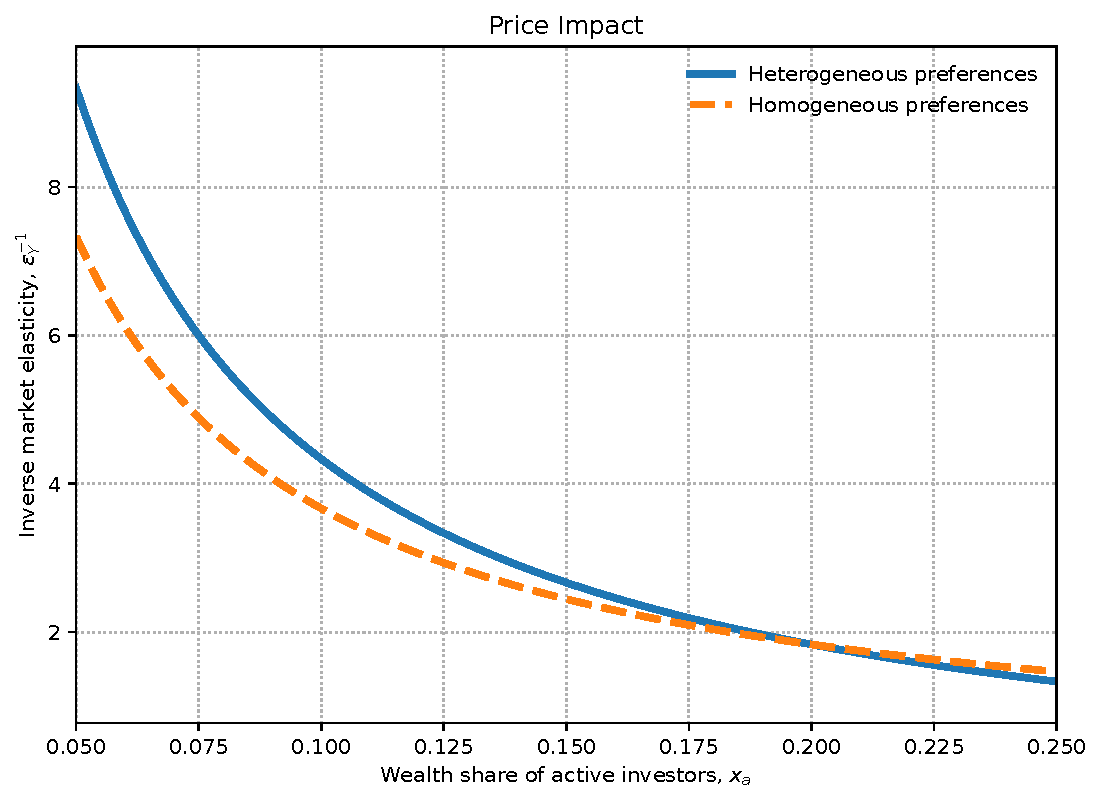
\includegraphics[width=\linewidth]{figures/price_impact_heterogeneity1.pdf}
        \caption{Homogeneous vs. heterogeneous preferences}
        \label{fig:impact_het_vs_hom}
    \end{subfigure}\hfill
    % --- Right: price impact vs w_1 for different \bar{\alpha}_p ---
    \begin{subfigure}[t]{0.48\textwidth}
        \centering
        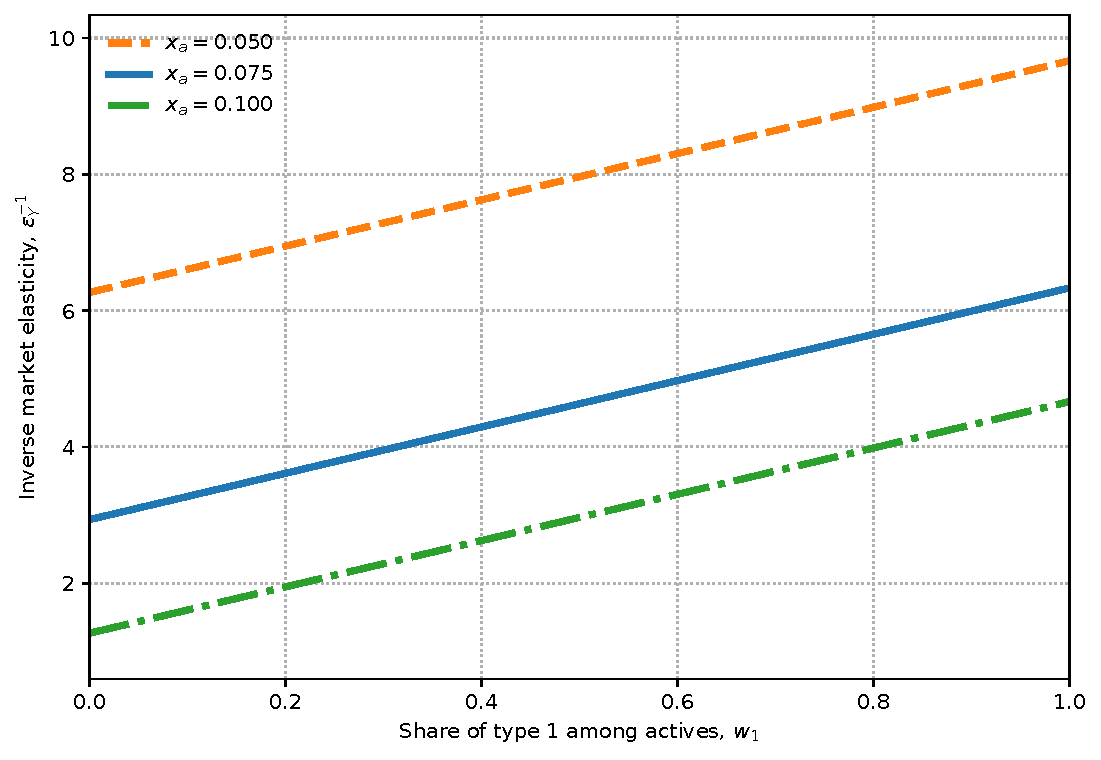
\includegraphics[width=\linewidth]{figures/price_impact_heterogeneity2.pdf}
        \caption{Role of wealth distribution of active investors}
        \label{fig:impact_vs_w1_by_alphap}
    \end{subfigure}
    \vspace{2mm}
    \caption{Price impact comparisons. Panel (a) compares heterogeneous and homogeneous preferences. Panel (b) shows the sensitivity of the price impact to wealth distribution among active investors when $J=2$ for different passive portfolio shares.}
    \label{fig:price_impact_comparison}
\end{figure}

% The right panel of Figure~\ref{fig:price_impact_comparison} highlights how the wealth split among active investors shapes price impact.
% With two active types ($J=2$) and $\gamma_1>\gamma_2$, the average active risk aversion is
% \[
% \mathbb{E}^u_t[\gamma_j] \;=\; w_{1,t}\gamma_1 + \bigl(1-w_{1,t}\bigr)\gamma_2,
% \qquad
% w_{1,t}\equiv \frac{x_{1,t}}{x_{a,t}}.
% \]
% When leverage constraints are slack ($x_{c,t}=0$), the passive investors’ optimal share satisfies
% \(
% \overline{\alpha}_{p,t}^{\mathrm{opt}}
% = 1 - x_{a,t}\,(\gamma_0-\mathbb{E}^u_t[\gamma_j])/\gamma
% \),
% hence
% \[
% \frac{\partial\,\overline{\alpha}_{p,t}^{\mathrm{opt}}}{\partial w_{1,t}}
% = \frac{x_{a,t}}{\gamma}\,(\gamma_1-\gamma_2) \;>\; 0.
% \]
% Thus, as the wealth share of the more risk-averse active type rises, $\mathbb{E}^u_t[\gamma_j]$ increases and the passive investor should optimally hold \emph{more} of the risky asset. If the passive portfolio is not adjusted, the deviation $\overline{\alpha}_{p,t}^{\mathrm{opt}}-\overline{\alpha}_{p,t}$ widens, worsening risk allocation and raising price impact—consistent with the upward shift shown in the right panel of Figure~\ref{fig:price_impact_comparison}.
Panel (b) of Figure~\ref{fig:price_impact_comparison} shows how the distribution of wealth across active investors shapes price impact. With two active types ($J=2$) and $\gamma_1>\gamma_2$, the average risk active aversion is
\[
\mathbb{E}^u_t[\gamma_j] \;=\; w_{1,t}\gamma_1 + \bigl(1-w_{1,t}\bigr)\gamma_2,
\qquad
w_{1,t}\equiv \frac{x_{1,t}}{x_{a,t}}.
\]
When leverage constraints are slack ($x_{c,t}=0$), the efficient passive share satisfies
\(
\overline{\alpha}_{p,t}^{\mathrm{opt}}
= 1 - x_{a,t}\,(\gamma_0-\mathbb{E}^u_t[\gamma_j])/\gamma,
\)
so holding $x_{a,t}$ fixed,
\[
\frac{\partial\,\overline{\alpha}_{p,t}^{\mathrm{opt}}}{\partial w_{1,t}}
= \frac{x_{a,t}}{\gamma}\,(\gamma_1-\gamma_2) \;>\; 0.
\]
Thus, as the wealth share of the more risk averse active type rises, $\mathbb{E}^u_t[\gamma_j]$ increases and the passive sector should optimally hold more of the risky asset. If the passive portfolio is not adjusted, the deviation $\overline{\alpha}_{p,t}^{\mathrm{opt}}-\overline{\alpha}_{p,t}$ widens, worsening risk allocation and raising price impact, consistent with the upward shift in the panel~(b) of Figure~\ref{fig:price_impact_comparison}.

% \paragraph{Leverage constraints.}
% Consider next the case where $x_{c,t} > 0$. In this case, the marginal investors are the \emph{unconstrained} active investors, so their risk-bearing capacity—measured by
% \[
% x_{u,t}\;\equiv\;x_{a,t}-x_{c,t},
% \]
% is crucial for determining the price impact.

% The left panel of Figure~\ref{fig:price_impact_leverage_constraints} shows the price impact as a function of the wealth share of active investors, $x_{a,t}=1-x_{0,t}$, with and without leverage constraints. To isolate the role of leverage constraints, we set $\gamma_0=\mathbb{E}_t^{u}[\gamma_j]$, so the term coming purely from preference heterogeneity drops out. As the share of active investors falls—e.g., after a negative aggregate shock when $\overline{\alpha}_{p,t}<1$—the price impact rises more sharply when leverage constraints bind. The reason is that constraints deplete the risk-bearing capacity of marginal investors (a smaller $x_{u,t}$), which raises price impact.

% The right panel of Figure~\ref{fig:price_impact_leverage_constraints} shows how the price impact responds to changes in the wealth share held by constrained investors, $x_{c,t}$, for a given $x_{a,t}$. Intuitively, the price impact is larger when a bigger share of active investors is constrained.
\paragraph{Leverage constraints.}
When some active investors are constrained ($x_{c,t}>0$), the marginal investors are the \emph{unconstrained} active agents, and their risk-bearing capacity,
\[
x_{u,t}\;\equiv\;x_{a,t}-x_{c,t},
\]
becomes the key determinant of price impact. The panel (a) of Figure~\ref{fig:price_impact_leverage_constraints} plots price impact against the active wealth share $x_{a,t}=1-x_{0,t}$, with and without binding constraints. To isolate the role of constraints, we set $\gamma_0=\mathbb{E}_t^{u}[\gamma_j]$, removing pure preference heterogeneity effects. As $x_{a,t}$ declines, e.g., after a negative aggregate shock when $\overline{\alpha}_{p,t}<1$, price impact rises more sharply under binding constraints because $x_{u,t}$ shrinks and the risk-bearing capacity of marginal investors is depleted. Panel (b) holds $x_{a,t}$ fixed and varies the constrained share $x_{c,t}$. The price impact increases monotonically with $x_{c,t}$. This is intuitive: price impact is larger when a larger share of active investors is constrained.

\begin{figure}[t]
    \centering
    % --- Left: with vs. without leverage constraints ---
    \begin{subfigure}[t]{0.48\textwidth}
        \centering
        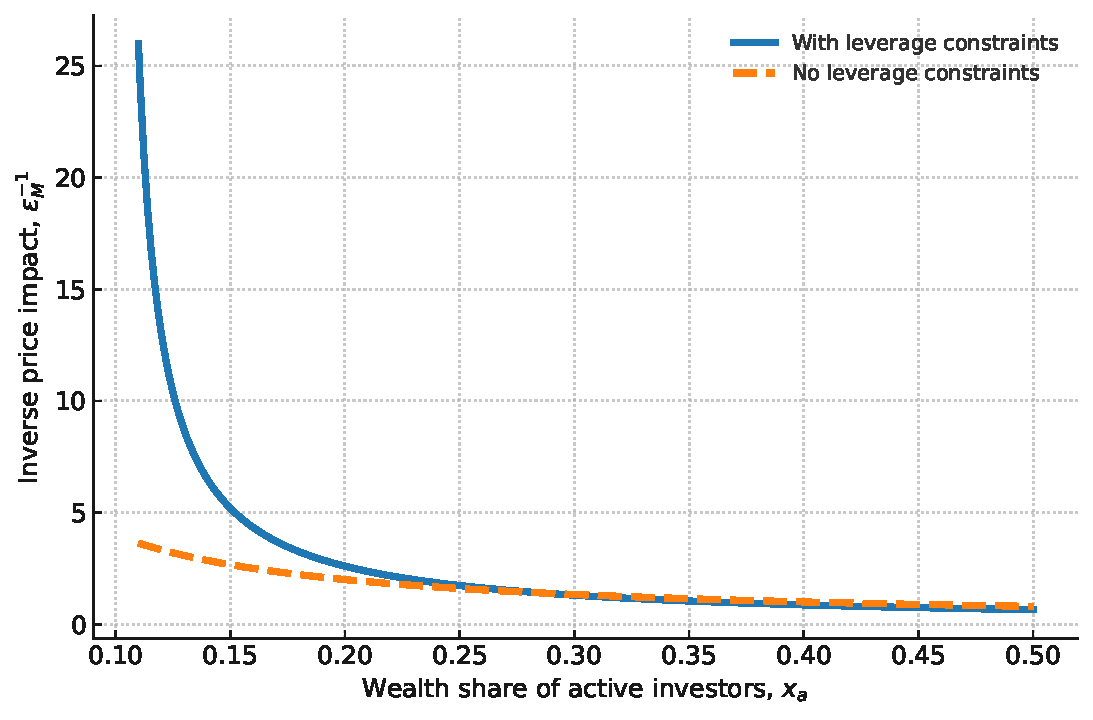
\includegraphics[width=\linewidth]{figures/price_impact_lev_constraints1.pdf}
        \caption{Role of leverage constraints \emph{(assumes $x_{c,t}=0.10$)}}
        % \label{fig:impact_het_vs_hom}
    \end{subfigure}\hfill
    % --- Right: price impact vs x_c for fixed x_a ---
    \begin{subfigure}[t]{0.48\textwidth}
        \centering
        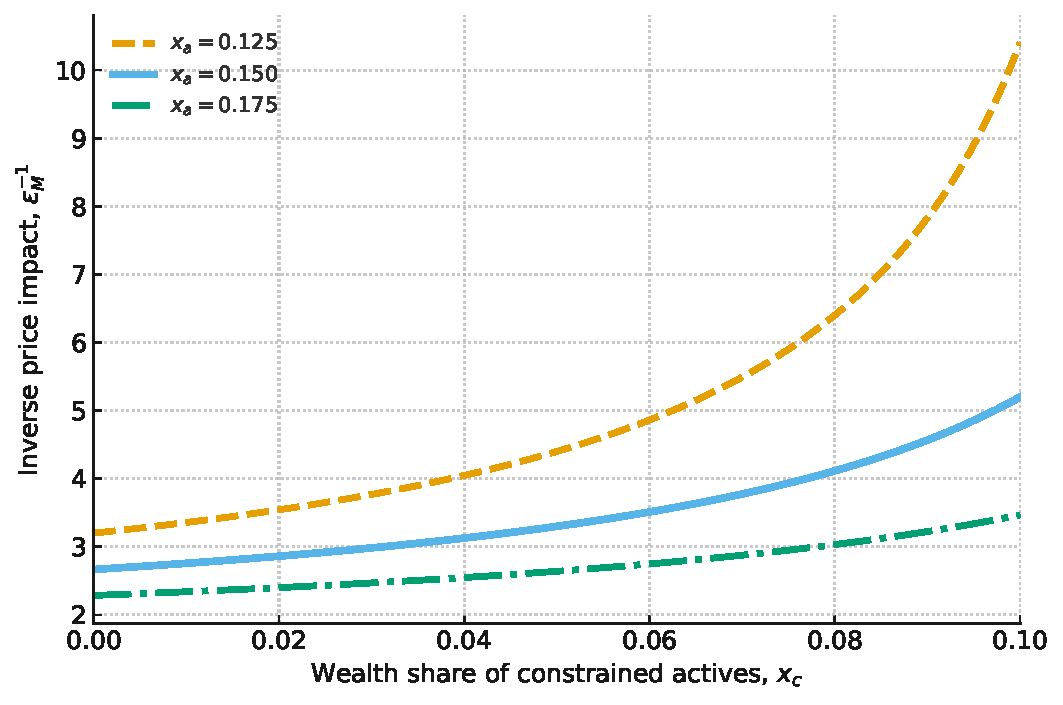
\includegraphics[width=\linewidth]{figures/price_impact_lev_constraints2.pdf}
        \caption{Varying the wealth share of constrained actives, $x_{c,t}$}
        % \label{fig:impact_vs_w1_by_alphap}
    \end{subfigure}
    \vspace{2mm}
    \caption{Price impact under leverage constraints. Panel (a) compares the cases with and without leverage constraints (holding $x_{c,t}=0.10$). Panel (b) plots the price impact as a function of $x_{c,t}$ for different values of $x_{a,t}$.}
    \label{fig:price_impact_leverage_constraints}
\end{figure}

% \paragraph{Taking stock.}
% Proposition~\ref{prop_elasticity_pref_heterog} enables us to characterize several key features of the aggregate market elasticity. First, the elasticity is \emph{finite} when risk is misallocated in the economy: small portfolio flows around a frictionless allocation have no first-order price impact. Second, preference heterogeneity tends to amplify price impact in bad times. As the wealth share of active investors falls, the efficient portfolio share of passive investors rises, widening the gap between efficient and actual portfolios. Third, leverage constraints further amplify price impact in bad times by shrinking $x_{u,t}$, the wealth share of marginal (unconstrained) investors. Therefore, aggregate market elasticity \emph{displays} rich state dependence in economies with heterogeneous investors and financial frictions.
\paragraph{Taking stock.}
Proposition~\ref{prop_elasticity_pref_heterog} clarifies the main determinants of aggregate market elasticity. The elasticity is \emph{finite} only when risk is misallocated: small portfolio flows around the frictionless allocation have no first-order price impact. Preference heterogeneity amplifies price impact in downturns because, as the active wealth share falls, the efficient passive share rises, widening the gap between efficient and actual portfolios. Binding leverage constraints further increase price impact by shrinking the marginal (unconstrained) risk-bearing capacity, $x_{u,t}$. Taken together, these forces imply rich state dependence of aggregate elasticity in economies with heterogeneous investors and financial frictions.



% The right panel of Figure~\ref{fig:price_impact_comparison} highlights the role of the wealth distribution among active investors. 
% Assuming $J = 2$ and $\gamma_1 > \gamma_2$, the average risk aversion among active investors is given by $\mathbb{E}^u[\gamma_j] = w_1 \gamma_1 + (1-w_1) \gamma_2$, where $w_1 = \frac{x_1}{x_a}$. 
% The figure shows that the price impact increases as the share of the more risk-averse active investor increases. 
% The reason is that as the average risk aversion of active investors increases, the passive investor should optimally hold more of the risky asset. 
% If the passive investor does not adjust its portfolio, this would worsen the allocation of risk, raising the price impact. 



% Several points are worth emphasizing. First, note that with heterogeneous active investors even in the case in which $ \overline{\alpha}_p=1 $, the aggregate elasticity is finite. As we show later in the next section, this effect is due to impact of flows on the risk-free rate. %\textcolor{red}{We probably need to say more here.}

% Second, assuming that the passive agents are more risk-averse than active investors, that is $ \gamma_{0}\ge\mathbb{E}^{u}[\gamma_{j}] $, with $ \psi>1 $, introducing preference heterogeneity attenuates the price response to flows, leading to more elastic markets relative to the economy without heterogeneity in Proposition~\ref{prop:elasticity_passive_demand}. This result is due to risk misallocation, as passive investors are effectively closer to their optimal portfolio when $\gamma_0  > \mathbb{E}^u[\gamma_j]$, for a given initial value $\overline{\alpha}_p < 1$.
% To see this point, let's compute the optimal portfolio share that investor $j = 0$ would choose if she was an active investor:
% % : for a given active wealth distribution $ x_a $, more risk-averse passive investors demand a higher risk premium for holding extra units of the risky asset, leading to a more depressed asset price response to flows.
% \begin{equation}
%     \overline{\alpha}_p^{optimal} = 1- x_a \left[ \frac{\gamma_0 - \mathbb{E}^a[\gamma_j]}{\gamma} \right],
% \end{equation}
% If type $j = 0$ investors have high risk aversion, then it is optimal for them to invest less than 100$\%$ in the risky asset. In this case, $\overline{\alpha}_p < 1$ is not an indication of risk misallocation, but it reflects the optimal risk sharing among investors. 
% It turns out that the elasticity will be positive if $\alpha_p < \overline{\alpha}_p^{optimal}$:
% \begin{equation}
% 	\varepsilon_M^{-1}=\left(1-\psi^{-1}\right) \frac{\gamma \sigma^{2}}{y_{0}(X)}\frac{\overline{\alpha}_{p,t}^{optimal}-\overline{\alpha}_{p}}{x_{a}}+\mathcal{O}\left(\epsilon^{2}\right).
% 	\end{equation}
% This shows that risk misallocation is again the key ingredient necessary to obtain a finite elasticity. Notice that a reduction in the wealth share of active investors raises the price impact by more in the presence of heterogeneous preferences, everything else constant. The reason is that a reduction in $x_a$ now raises the optimal portfolio share of passive investors. 
% Optimal risk sharing implies they should hold more of the risky asset when $x_a$ is low, which is typically after a negative aggregate shock. For a given level of $\overline{\alpha}_p$, this implies that there is more risk misallocation when $x_a$ is low, that is, $\overline{\alpha}_p$ is further away from the optimal.




% Finally, from Equation~\eqref{eq:elasticity_pref_heterog}, we see that the price impact of flows depends not only on the wealth share of active investors $ x_a $ as before, but also on the wealth distribution among active investors through $ \E^u[\gamma_j] $. This results reiterates the importance of heterogeneity among financial intermediaries that active investors in our model represent (e.g., \citealp{Veronesi/2019};  \citealp{Kargar/2021}). 
% % Also as before, in states in which active investors are undercapitalized, the aggregate market become more inelastic.

% In Figure~\ref{Fig:elasticity_pref_het}, we plot inverse aggregate elasticity for the case with one passive and two active investors ($ J=3 $) with $ \gamma_{0}\ge\gamma_{1}>\gamma_{2} $. In this economy, the two key state variables are the wealth share of active investors, $ x_a $, and the wealth share the most risk-tolerant active investor (agent 2) among active investors, $ w $:
% \begin{equation}\label{eq:state-vars-3agents}
% x_a=1-x_0,\qquad w=\frac{x_2}{x_a}.
% \end{equation}
% \begin{figure}[!t]
% 	\centering
% 	
\includegraphics[width=\textwidth]{./figures/elasticity_heterog.pdf}
% 	\caption{Price impact: passive demand and preference heterogeneity.}
% 	\label{Fig:elasticity_pref_het}
% \end{figure}
% From Figure~\ref{Fig:elasticity_pref_het}, we see that as the active investors become less capitalized and $ x_a $ declines, market become more inelastic. Moreover, as less risk averse active investors become less capitalized and $ w $ goes down, we see a larger price impact from passive flows. 
% %\begin{itemize}
% %	\item Discuss connections with \cite{garleanu2015young}.
% %	\item \sout{Discuss connection with} \cite{Veronesi/2019}.
% %\end{itemize}

% \subsection{Leverage constraints}

% % We consider next the case where investors have heterogeneous preferences and they are subject to leverage constraints. 
% % In Proposition~\ref{prop:elasticity_leverage_constraint}, we derive the aggregate market elasticity when heterogeneous active investors also face leverage constraints.
% % \begin{prop}[Aggregate elasticity: leverage constraints]\label{prop:elasticity_leverage_constraint}
% % 	Suppose $\rho>\left(1-\psi^{-1}\right)\left( \mu - \frac{\gamma\|\sigma\|^2}{2}  \right)$. When active investors have heterogeneous preferences and also face leverage constraints in \eqref{eq:leverage_constraint}, the inverse aggregate market elasticity, $ 1/\varepsilon_M $, is given by:
% % 	%\begin{small}
% % 		\begin{align}		
% % 		\varepsilon_M^{-1}&=
% % 		\left(1-\psi^{-1}\right) \frac{\gamma \sigma^{2}}{y_{0}(X)}\left[\frac{(1-x_c)(1-\overline{\alpha}_{p})}{x_{u}}-\frac{\gamma_{0}-\mathbb{E}^{u}[\gamma_{j}]}{\gamma} -\frac{x_c(\frac{\overline{\sigma}}{\sigma}-1)}{x_u}\right]
% % 		%\left(1-\psi^{-1}\right) \frac{\gamma \sigma^{2}}{y_{0}(X)}\left[\frac{1-\overline{\alpha}_{p}}{x_{u}}-\frac{\gamma_{0}-\mathbb{E}^{u}\left[\gamma_{j}\right]}{\gamma}\right] \nonumber\\
% % 		+\mathcal{O}\left(\epsilon^{2}\right).	\label{eq:elasticity_leverage_constraint}		
% % 		%&+\left(1-\psi^{-1}\right) \frac{\gamma \sigma^{2}}{y_{0}(X)}\left[\frac{\mathbb{E}^{u}\left[\gamma_{k}\right]-\mathbb{E}^{c}\left[\gamma_{k}\right]}{\gamma x_{u}}+\frac{\gamma \sigma\left(1-\psi^{-1}\right)}{2 y_{0}(X)} \frac{\gamma_{0}-\mathbb{E}^{u}\left[\gamma_{k}\right]}{\gamma}+\frac{\overline{\alpha}_{p}-\frac{\overline{\sigma}}{\sigma}}{x_{u}}\right] x_{c}+\mathcal{O}\left(\epsilon^{2}\right),	\label{eq:elasticity_leverage_constraint}		
% % 		\end{align}						
% % 	%\end{small}		
% % \end{prop}
% % \begin{proof}
% % 	See Appendix~\ref{app:prop_elasticity_leverage_constraint}.
% % \end{proof}
% % We highlight several points from Proposition~\ref{prop:elasticity_leverage_constraint}. First, note than when all active agents are unconstrained, i.e., $ x_c=0 $, we get the price impact from Proposition~\ref{prop_elasticity_pref_heterog}. Similar to the case with heterogeneous investors, the aggregate elasticity is finite when $ \overline{\alpha}_p=1 $.



% % \begin{figure}[!t]
% % 	\centering
% % 	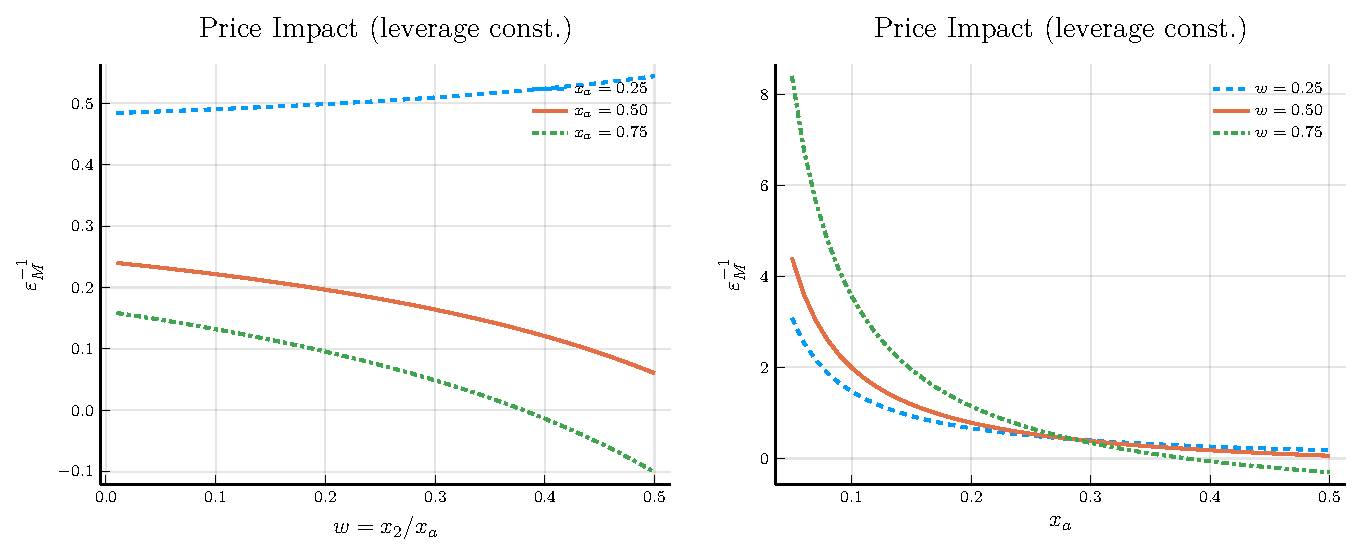
\includegraphics[width=\textwidth]{figures/elasticity_lev-const.pdf}
% % 	\caption{Price impact: leverage constraints.}
% % 	\label{Fig:elasticity_leverage_const}
% % \end{figure}

% As in the previous two cases, risk misallocation plays an important role. The optimal portfolio share of type $j = 0$ investors, i.e. the portfolio they would choose if they were active, is given by
% \begin{equation}
%     \overline{\alpha}_{p,t}^{\mathrm{opt}} = 1 -\frac{x_u}{1-x_c}\frac{\gamma_0-\mathbb{E}^u[\gamma_j] }{\gamma} - \frac{x_c(\frac{\overline{\sigma}}{\|\sigma\|}-1)  }{1-x_c}.
% \end{equation}
% Plugging the formula for the optimal portfolio share in the expression for the aggregate market elasticity, we obtain
% \begin{equation}
% 	\varepsilon_M^{-1}=\left(1-\psi^{-1}\right) \frac{\gamma \sigma^{2}}{y_{0}(X)}\frac{\overline{\alpha}_{p,t}^{\mathrm{opt}}-\overline{\alpha}_{p}}{x_{a}}(1-x_c)+\mathcal{O}\left(\epsilon^{2}\right).
% 	\end{equation}
% As before, the market elasticity is finite and positive when $\overline{\alpha}_p$ is below its optimal level. The optimal portfolio now depends on the average risk aversion of unconstrained agents, the leverage constraint, and the entire distribution among active investors. 
% Figure~\ref{Fig:elasticity_frictions} illustrates the behavior of the market elasticity in the presence of leverage constraints. The left panel shows the price impact for different values of $w = x_2/x_a$, that is, the share of wealth of the low risk aversion investor among active investors. 
% The right panel shows the inverse elasticity as a function of the wealth share of active investors. 


% % Let us consider an example to help simplify the exposition. Suppose there are three agents ($ J=3 $), one passive and two active investors, with risk aversions $ \gamma_{0}=\gamma_1>\gamma_2 $. As before, $ j=0 $ represents the passive investor. For simplicity, also assume $ \overline{\alpha}_p=1 $ and $ \overline{\sigma}=\sigma $. First, suppose agent 2 is unconstrained, so that $ x_u=x_1+x_2 $ and $ x_c=0 $. In this case, only the second term in the square bracket in Equation~\eqref{eq:elasticity_leverage_constraint} is non-zero, leading to a \textit{negative} price impact of the asset flows:
% % \[\epsilon_M^{-1}=
% % -\left(1-\psi^{-1}\right)\frac{\gamma\sigma^2}{y_0(X)}\frac{\gamma_0-\E^u[\gamma_{j}]}{\gamma}<0.\]

% % Now suppose agent 2 faces binding leverage constraint, so that  $ x_u=x_1 $, and $ x_c=x_2 $. In this case we have 
% % \[ \E^u\left[\gamma_k\right]=\gamma_{0}>\E^c\left[\gamma_k\right]=\gamma_2.\]
% % Note that, in this case, only the first term in the square bracket in the second line of Equation~\eqref{eq:elasticity_leverage_constraint} is positive and all other terms are zero. So, the inverse aggregate elasticity simplifies to 
% % \[\varepsilon_M^{-1}=\left(1-\psi^{-1}\right) \frac{\left(\gamma_{0}-\gamma_{2}\right)\sigma^2}{y_{0}(X) x_{u}}>0,\]
% % and flows lead to an increase in the price-dividend ratio. Thus, the introduction of the constrained investor leads to a \textit{positive} price response to flows and a finite aggregate elasticity. This result shows that even when passive investors are fully invested in the risky asset, the presence of binding portfolio constraints can lead to finite market elasticity. This is again due to 
% % % \textcolor{red}{needs to be completed $ \dots $}%risk misallocation: when the leverage constraint binds to investor 2, the more risk averse need to have higher 

% \begin{figure}[!t]
% 	\centering
% 	
\includegraphics[width=\textwidth]{figures/elasticity_frictions.pdf}
% 	\caption{Decomposition of the inverse aggregate market elasticity.}
% 	\label{Fig:elasticity_frictions}
% \end{figure}


% %\textcolor{red}{
% %\begin{itemize}
% %	\item Need to dissect the extra term from leverage constraint. 
% %	\item \sout{Perhaps consider 3 types: one passive with $ \gamma_{0} $, and two active with $ \gamma_0=\gamma_1>\gamma_2 $. For simplicity can also assume $ \overline{\alpha}_p=1 $ and $ \overline{\sigma}=\sigma $.}
% %	\item \sout{To get intuition, look at components of elasticity separately: $ \dfrac{\partial\eta_2}{\partial F} $ and $ \dfrac{\partial r_2}{\partial F} $.}
% %	\item \sout{look at the impact of flows on the risk premium $\eta\sigma$. This has three components. $r$, risk premium, and volatility.}
% %	\item \sout{would like to see the response of risk premium}
% %	\item also response of volatility
% %\end{itemize}}
% %\begin{prop}\label{prop:elasticity_second_order}
% %	The inverse aggregate market elasticity $ 1/\varepsilon_M $ is given under the following three conditions:
% %	\begin{enumerate}[(i)]
% %		\item \textbf{Passive demand:} If there is no preference heterogeneity and active investors do not face leverage constraint, the inverse elasticity is given by:
% %		\[\frac{1}{p(X, \epsilon)} \frac{\partial p(X, \epsilon)}{\partial F(X, \epsilon)}=\left(1-\psi^{-1}\right) \frac{\gamma \sigma^{2}}{y_{0}(X)} \frac{1-\bar{\alpha}_{p}}{x_{1}}+\mathcal{O}\left(\epsilon^{2}\right).\]
% %		\item \textbf{Preference heterogeneity:} If active investors have heterogeneous risk aversions but face no leverage constraint, the inverse elasticity is given by:
% %		\[\frac{1}{p(X, \epsilon)} \frac{\partial p(X, \epsilon)}{\partial F(X, \epsilon)}=\left(1-\psi^{-1}\right) \frac{\gamma \sigma^{2}}{y_{0}(X)}\left[\frac{1-\bar{\alpha}_{p}}{x_{a}}-\frac{\hat{\gamma}_{0}-\mathbb{E}^{u}\left[\hat{\gamma}_{j}\right]}{\gamma}\right]+\mathcal{O}\left(\epsilon^{2}\right),\]
% %		where $ \mathbb{E}^u\left[ \hat{\gamma}_j\right] \equiv\sum_{j\in\mathcal{J}^u} \frac{x_j}{x_u} \hat{\gamma}_j, $ and $ x_{a} \equiv 1-x_{0} $ denotes the wealth share of active investors.
% %		\item \textbf{Leverage constraints:} When active investors have heterogeneous preferences and also face leverage constraints, the inverse market elasticity is given by:
% %		\begin{small}
% %			\begin{align*}
% %				\frac{1}{p(X, \epsilon)} \frac{\partial p(X, \epsilon)}{\partial F(X, \epsilon)}&=
% %				\left(1-\psi^{-1}\right) \frac{\gamma \sigma^{2}}{y_{0}(X)}\left[\frac{1-\bar{\alpha}_{p}}{x_{u}}-\frac{\hat{\gamma}_{0}-\mathbb{E}^{u}\left[\hat{\gamma}_{j}\right]}{\gamma}\right] \\
% %				&+\left(1-\psi^{-1}\right) \frac{\gamma \sigma^{2}}{y_{0}(X)}\left[\frac{\mathbb{E}^{u}\left[\hat{\gamma}_{k}\right]-\mathbb{E}^{c}\left[\hat{\gamma}_{k}\right]}{\gamma x_{u}}+\frac{\gamma \sigma\left(1-\psi^{-1}\right)}{2 y_{0}(X)} \frac{\gamma_{0}-\mathbb{E}^{u}\left[\hat{\gamma}_{k}\right]}{\gamma}+\frac{\bar{\alpha}_{p}-\frac{\bar{\sigma}}{\sigma}}{x_{u}}\right] x_{c}\\
% %				&+\mathcal{O}\left(\epsilon^{2}\right),			
% %			\end{align*}						
% %		\end{small}		
% %	where $ \textcolor{red}{\mathbb{E}^c\left[ \hat{\gamma}_k\right] \equiv\sum_{k\in\mathcal{J}^c} \frac{x_k}{x_c} \hat{\gamma}_j.} $
% %	\end{enumerate}
% %\end{prop}
% %\begin{proof}
% %	See Appendix~\ref{app:prop_second_order_elasticity}.
% %\end{proof}

% %\begin{itemize}
% %    \item \sout{Define flows}
% %    \item \sout{Show opposite effects on interest rate and risk premium}
% %    \item \sout{Infinite elasticity up to first-order}
% %    \item \sout{You need to go to second-order}
% %    \item \sout{Three cases in second-order}
% %    \begin{itemize}
% %        \item \sout{Passive investment / risk concentration}
% %        \item \sout{Heterogeneity}
% %        \item \sout{Leverage constraints}
% %    \end{itemize}
% %	\item Discussion of Prop 2    
% %\end{itemize}

% % \section{Aggregate Elasticity and Excess Volatility}
% % \begin{itemize}
% % 	\item Quantitative implications
% % 	\begin{itemize}
% % 		\item Connection between volatility and elasticity
% % 	\end{itemize}
	
% % 	\begin{equation}
% % 		\sigma_p(x,\overline{\alpha}_p) = \frac{p_x}{p} \sigma_x + \frac{p_{\overline{\alpha}_p}}{p} \sigma_{\overline{\alpha}_p}
% % 	\end{equation}
	
	
% % 	\begin{equation}
% % 		\frac{d p}{p} = \frac{1}{\varepsilon_M(X)} dF
% % 	\end{equation}
	
% % \end{itemize}
% % In Proposition~\ref{prop:volatility-flow}, we assess the impact of flows on return volatility $ \sigma_{R} $.
% % \begin{prop}[Portfolio flows and volatility]\label{prop:volatility-flow}
% % 	The impact of asset flows on return volatility is
% % 	\begin{equation}\label{eq:volatility-flow}
% % 		\frac{\partial\sigma_{R}(X,\epsilon)}{\partial F(X,\epsilon)}=-\left(1-\psi^{-1}\right) \frac{\gamma \sigma^{2}}{2 y_{0}(X)}\sigma\left(\hat{\gamma}_{0}-\mathbb{E}^{u}\left[\hat{\gamma}_{k}\right]\right)
% % 	\end{equation}
% % \end{prop}
% % We used $ \sigma_{R,1}(X)=0 $ and $ \sigma_{R,2}(X)=-\sigma_{y,2}(X). $
% % \begin{proof}
% % 	See Appendix~\ref{app:prop_volatility-flow}.
% % \end{proof}

% % \section{Discussion and Main Lessons}
% % We draw four main lessons from the results in Propositions~\ref{prop:elasticity_passive_demand}--\ref{prop:volatility-flow}.
% % \begin{lesson}[The role of interest rates]
% % 	Regardless of how constrained agents are, in the unit EIS case ($ \psi=1 $), the aggregate market elasticity is infinite. 
% % \end{lesson}
% % We need $ \psi>1 $ to obtain positive price impact of flow shocks.

% % \begin{lesson}[State dependence]
% % 	The aggregate elasticity is time-varying and state-dependent.
% % \end{lesson}
% % Market elasticity is function of economy's aggregate sate variables, capturing time-varying investment opportunities. 

% % \begin{lesson}[Risk misallocation]
% % 	Markets are inelastic when risk is misallocated in the economy.
% % \end{lesson}
% % Conjecture: with perfect risk sharing, there is no price impact.

% % \begin{lesson}[Volatility]
% % 	Volatility depends on both market elasticity and portfolio flow shocks.
% % \end{lesson}





% % \section{Decomposition of the Aggregate Market Elasticity}
% % Equipped with the definition of (inverse) market elasticity in Equation~\eqref{eq:elasticity-y2}, we can use the pricing condition in \eqref{eq:pricing_cond} to decompose the price impact into three terms: the impact of flows on (i) the risk-free rate, (ii) the risk-premium, and (iii) the drift of the asset price. This decomposition is given by
% % \begin{equation}\label{eq:elasticity-decomp}
% % 	\varepsilon_M^{-1}=-\frac{1}{y_0(X)}\left[\frac{\partial r_2(X)}{\partial\hat{\alpha}_p}+
% % 	\frac{\partial\pi_2(X)}{\partial\hat{\alpha}_p}-
% % 	\frac{\partial\mu_{P,2}(X)}{\partial\hat{\alpha}_p}\right]\frac{\epsilon}{x_0},
% % \end{equation}
% % where $ \mu_{P,t}=\mu-\mu_{y,t}-\sigma_{y,t}\sigma_{R,t} $ is the drift of the risky asset price $ P_t $, and $ \pi_t=\sigma_{R,t}\eta_t $ is the risk premium. The second-order correction for the risk premium and the asset price drift can be derived easily:
% % \begin{align}
% % 	\pi_{2}(X)&=-\eta_{0}(X) \sigma_{y, 2}(X)+\eta_{2}(X) \sigma\\
% % 	\mu_{P,2}(X)&=-\mu_{y,2}(X)-\sigma\sigma_{y,2}(X),
% % \end{align}
% % where we use the fact that $ \sigma_{y,0}(X)=\sigma_{R,0}(X)=\sigma_{y,1}(X)=\sigma_{R,1}(X)=0 $. We again consider the three cases we discussed in the previous section.

% % \begin{figure}[!t]
% % 	\centering
% % 	
\includegraphics[width=\textwidth]{./figures/p_impact_het_decomp.pdf}
% % 	\caption{Decomposition of the inverse aggregate market elasticity.}
% % 	\label{Fig:elasticity_decomp}
% % \end{figure}
% % \textcolor{red}{discuss the interpretation of the three terms: interest rate, risk premium, and drift of the price.}


% % \subsection{Passive demand}
% % In the absence of investor heterogeneity (i.e., $ \hat{\gamma}_j=0 $ for all $ j $) and leverage constraints (that is $ x_c=0 $), we have $ \mu_{P,2}(X)=-\mu_{y,2}(X)=0 $. In this case, $ \sigma_{y, 2}(X)=\eta_{2}(X)=0 $ and therefore, $ \pi_2(X)= 0$. Thus, we have $ r_2(X)=y_2(X) $ and  
% % \begin{align*}
% % 	\frac{\partial\mu_{P,2}(X)}{\partial\hat{\alpha}_p}=0,
% % 	\qquad\frac{\partial\pi_{2}(X)}{\partial\hat{\alpha}_p}=0,
% % 	\qquad\frac{\partial r_{2}(X)}{\partial\hat{\alpha}_p}=\frac{\partial y_{2}(X)}{\partial\hat{\alpha}_p}.
% % \end{align*}
% % Therefore, the aggregate elasticity is
% % \[\varepsilon_M^{-1}=-\frac{1}{y_0(X)}\frac{\partial r_2(X)}{\partial \hat{\alpha}_p}\frac{\epsilon}{x_0}=
% % \left(1-\psi^{-1}\right) \frac{\gamma \sigma^{2}}{y_{0}(X)} \frac{1-\overline{\alpha}_{p}}{x_{a}}+\mathcal{O}\left(\epsilon^{2}\right)\]
% % which is exactly the expression for the aggregate market elasticity in Proposition~\ref{prop:elasticity_passive_demand}. 

% % So, in the case where all investors have the same preferences and do not face leverage constraints, the market elasticity is entirely determined by the second-order impact of flows on the risk-free rate.

% % \textcolor{red}{mention everyone has the same risk aversion.}

% % \subsection{Investor heterogeneity}
% % In this case, the impact of flows can be summarized as
% % \begin{small}
% % 	\begin{align*}
% % 		-\frac{\partial\mu_{P,2}(X)}{\partial\hat{\alpha}_p}\frac{\epsilon}{x_0}&=\left(1-\psi^{-1}\right)\frac{\gamma\sigma^2}{2y_0(X)}(\gamma-1)\sigma^2\left(\frac{\gamma_{0}-\mathbb{E}^{u}\left[\gamma_{j}\right]}{\gamma}\right)
% % 		+\left(1-\psi^{-1}\right)\frac{\gamma \sigma^{2}}{2 y_{0}(X)}\sigma^2\left(\frac{\gamma_{0}-\mathbb{E}^{u}\left[\gamma_{j}\right]}{\gamma}\right),\\
% % 		\frac{\partial\pi_{2}(X)}{\partial\hat{\alpha}_p}\frac{\epsilon}{x_0}&=-\left(1-\psi^{-1}\right) \frac{\gamma \sigma^{2}}{2 y_{0}(X)}(1+\gamma)\sigma^2\left(\frac{\gamma_{0}-\mathbb{E}^{u}\left[\gamma_{j}\right]}{\gamma}\right)-\frac{\gamma\sigma^2}{x_a}\E^u[\hat{\gamma}_j]\epsilon,\\
% % 		\frac{\partial r_{2}(X)}{\partial\hat{\alpha}_p}\frac{\epsilon}{x_0}&=
% % 		-\left(1-\psi^{-1}\right)\frac{\gamma\sigma^2}{2y_0(X)}(\gamma-1)\sigma^2\left(\frac{\gamma_{0}-\mathbb{E}^{u}\left[\gamma_{j}\right]}{\gamma}\right)
% % 		-\left(1-\psi^{-1}\right)\gamma\sigma^2\left[\frac{1-\overline{\alpha}_{p}}{x_{a}}-\frac{\gamma_{0}-\mathbb{E}^{u}\left[\gamma_{j}\right]}{\gamma}\right]\\
% % 		&\quad+\left(1-\psi^{-1}\right)\frac{\gamma \sigma^{2}}{2 y_{0}(X)}\gamma\sigma^2\left(\frac{\gamma_{0}-\mathbb{E}^{u}\left[\gamma_{j}\right]}{\gamma}\right)+\frac{\gamma\sigma^2}{x_a}\E^u[\hat{\gamma}_j]\epsilon.
% % 	\end{align*}
% % \end{small}
% % \textcolor{red}{Discuss the intuition.}

% % \subsection{Leverage constraints}
% % In this case, the impact of flows can be summarized as
% % \begin{small}
% % 	\begin{align*}
% % 		-\frac{\partial\mu_{P,2}(X)}{\partial\hat{\alpha}_p}\frac{\epsilon}{x_0}&=\left(1-\psi^{-1}\right)\frac{\gamma\sigma^2}{2y_0(X)}(\gamma-1)\sigma^2\left(\frac{\gamma_{0}-\mathbb{E}^{u}\left[\gamma_{j}\right]}{\gamma}\right)
% % 		+\left(1-\psi^{-1}\right)\frac{\gamma \sigma^{2}}{2 y_{0}(X)}\sigma^2\left(\frac{\gamma_{0}-\mathbb{E}^{u}\left[\gamma_{j}\right]}{\gamma}\right),\\
% % 		\frac{\partial\pi_{2}(X)}{\partial\hat{\alpha}_p}\frac{\epsilon}{x_0}&=
% % 		-\left(1-\psi^{-1}\right) \frac{\gamma \sigma^{2}}{2 y_{0}(X)}\left(\gamma+\frac{(1-\gamma)x_c+1-x_0}{x_u}\right)\sigma^2\left(\frac{\gamma_{0}-\mathbb{E}^{u}\left[\gamma_{j}\right]}{\gamma}\right)-\frac{\gamma\sigma^2}{x_a}\E^u[\hat{\gamma}_j]\epsilon,\\
% % 		\frac{\partial r_{2}(X)}{\partial\hat{\alpha}_p}\frac{\epsilon}{x_0}&=
% % 		-\left(1-\psi^{-1}\right)\frac{\gamma\sigma^2}{2y_0(X)}(\gamma-1)\sigma^2\left(\frac{\gamma_{0}-\mathbb{E}^{u}\left[\gamma_{j}\right]}{\gamma}\right)\\
% % 		&\quad-\left(1-\psi^{-1}\right)\gamma\sigma^2\left[\frac{1-\overline{\alpha}_{p}}{x_{a}}-\frac{\gamma_{0}-\mathbb{E}^{u}\left[\gamma_{j}\right]}{\gamma}\right]\\
% % 		&\quad-\left(1-\psi^{-1}\right) \frac{\gamma \sigma^{2}}{y_{0}(X)}\left[\frac{\mathbb{E}^{u}\left[\gamma_{k}\right]-\mathbb{E}^{c}\left[\gamma_{k}\right]}{\gamma x_{u}}+\frac{\gamma \sigma\left(1-\psi^{-1}\right)}{2 y_{0}(X)} \frac{\gamma_{0}-\mathbb{E}^{u}\left[\gamma_{k}\right]}{\gamma}+\frac{\overline{\alpha}_{p}-\frac{\overline{\sigma}}{\sigma}}{x_{u}}\right] x_{c}\\
% % 		&\quad+\left(1-\psi^{-1}\right)\frac{\gamma \sigma^{2}}{2 y_{0}(X)}\left(\gamma+\frac{(1-\gamma)x_c+x_c}{x_u}\right)\sigma^2\left(\frac{\gamma_{0}-\mathbb{E}^{u}\left[\gamma_{j}\right]}{\gamma}\right)+\frac{\gamma\sigma^2}{x_a}\E^u[\hat{\gamma}_j]\epsilon.
% % 	\end{align*}
% % \end{small}
% % \textcolor{red}{Discuss the intuition.}

        
% % \section{Price impact and risk misallocation}

% % \paragraph{No leverage constraints.} Assume there is no leverage constraints. Investor $j$'s demand for risk, for $j = 1,\ldots, J$, is given by 
% % \begin{equation}
% %     \sigma_j(X) = \sigma + \sigma \left[  \sum_{k=1}^J \frac{x_k}{1-x_0} \hat{\gamma}_k - \hat{\gamma}_j  - \frac{\hat{\alpha}_p x_0}{1-x_0}\right] \epsilon + \mathcal{O}(\epsilon^2).
% % \end{equation}

% % Therefore, if investor $j = 0$ were active (i.e., $x_0=0$), the optimal risk allocation would satisfy:
% % \begin{equation}
% %     \sigma_j(X) = \sigma + \sigma \left[  \sum_{k=0}^J x_k \hat{\gamma}_k - \hat{\gamma}_j  \right] \epsilon + \mathcal{O}(\epsilon^2).
% % \end{equation}

% % The passive investor's actual risk exposure is given by $\sigma_0(X) = \sigma + \hat{\alpha}_p \sigma \epsilon$. Hence, the actual risk exposure coincides with the optimal risk exposure if
% % \begin{align}
% %     \hat{\alpha}_p^{optimal} &=  \sum_{k=1}^J x_k \hat{\gamma}_k - (1-x_0) \hat{\gamma}_0 \\
% %     &= - x_a \left[ \frac{\gamma_0 - \mathbb{E}^a[\gamma_j]}{\gamma} \right],
% % \end{align}
% % where $\mathbb{E}^a[\gamma_j] \equiv \sum_{k=1}^J \frac{x_k}{1-x_0} \gamma_k$ and $x_a\equiv(1-x_0)$.

% % The price impact with heterogeneous preferences is given by
% % \begin{equation}
% % 	%\frac{1}{p(X, \epsilon)} \frac{\partial p(X, \epsilon)}{\partial F(X, \epsilon)}
% % 	\varepsilon_M^{-1}=\left(1-\psi^{-1}\right) \frac{\gamma \sigma^{2}}{y_{0}(X)}\left[\frac{1-\overline{\alpha}_{p}}{x_{a}}-\frac{\gamma_{0}-\mathbb{E}^{a}[\gamma_{j}]}{\gamma}\right]+\mathcal{O}\left(\epsilon^{2}\right),
% % \end{equation}

% % Using the fact that $\overline{\alpha}_p = 1 + \hat{\alpha}_p \epsilon$ and $x_a = 1-x_0$, we obtain that the price impact is given by
% % \begin{equation}
% % 	%\frac{1}{p(X, \epsilon)} \frac{\partial p(X, \epsilon)}{\partial F(X, \epsilon)}
% % 	\varepsilon_M^{-1}=\left(1-\psi^{-1}\right) \frac{\gamma \sigma^{2}}{y_{0}(X)}\left[-\frac{\hat{\alpha}_{p}}{1-x_0}-\frac{\gamma_{0}-\mathbb{E}^{a
% %  }[\gamma_{j}]}{\gamma}\right]+\mathcal{O}\left(\epsilon^{2}\right) \approx 0.
% % \end{equation}

% % Notice that we can write the price impact as follows:
% % \begin{equation}
% % 	%\frac{1}{p(X, \epsilon)} \frac{\partial p(X, \epsilon)}{\partial F(X, \epsilon)}
% % 	\varepsilon_M^{-1}=\left(1-\psi^{-1}\right) \frac{\gamma \sigma^{2}}{y_{0}(X)}\frac{\overline{\alpha}_p^{opt}-\overline{\alpha}_{p}}{x_{a}}+\mathcal{O}\left(\epsilon^{2}\right),\label{eq:price-impact-het-misallocation}
% % \end{equation}

% % \paragraph{Leverage constraints.} With leverage constraints, the risk exposure is given by
% % \begin{equation}
% %     \sigma_j(X) = \sigma_{j,0}(X) +\|\sigma\|\min\left\{ \sum_{k\in\mathcal{J}^u} \frac{x_k}{x_u} \hat{\gamma}_k -\left(\frac{\hat{\alpha}_p  x_0+\frac{\hat{\sigma}}{\|\sigma\|} x_c }{1-x_0-x_c}\right)- \hat{\gamma}_j  ,\frac{\hat{\sigma}}{\|\sigma\|}  \right\}\epsilon + \mathcal{O}(\epsilon^2).
% % \end{equation}

% % This reflects the effects of two frictions: leverage constraints and the presence of passive investors. To isolate the role of each friction, assume there is no passive investors, so the risk exposure is given by 
% % \begin{equation}
% %     \sigma_j(X) = \sigma_{j,0}(X) +\|\sigma\|\min\left\{ \sum_{k=0}^{J_u} \frac{x_k}{1-x_c} \hat{\gamma}_k -\frac{\frac{\hat{\sigma}}{\|\sigma\|} x_c }{1-x_c}- \hat{\gamma}_j  ,\frac{\hat{\sigma}}{\|\sigma\|}  \right\}\epsilon + \mathcal{O}(\epsilon^2),
% % \end{equation}
% % where we assume that investors $j \in \{0, 1,\ldots, J_u\}$ are unconstrained given the current state.

% % Investor $j$ would be holding his privately optimal portfolio if
% % \begin{align}
% %     \hat{\alpha}_p^{opt} \epsilon &= \left[\sum_{k=0}^{J_u} \frac{x_k}{1-x_c} \hat{\gamma}_k -\frac{\frac{\hat{\sigma}}{\|\sigma\|} x_c }{1-x_c}- \hat{\gamma}_0\right] \epsilon\\
% %      &= -\frac{x_u}{1-x_c}\frac{\gamma_0-\mathbb{E}^u[\gamma_j] }{\gamma} - \frac{\frac{\hat{\sigma}}{\|\sigma\|} x_c }{1-x_c},
% % \end{align}
% % where $x_u=1-x_c - x_0.$
% % The price impact is given by
% % \begin{align}		
% % 		\varepsilon_M^{-1}&=
% % 		\left(1-\psi^{-1}\right) \frac{\gamma \sigma^{2}}{y_{0}(X)}\left[\frac{(1-x_c)(1-\overline{\alpha}_{p})-x_c(\frac{\overline{\sigma}}{\sigma}-1)}{1-x_c -x_0}-\frac{\gamma_{0}-\mathbb{E}^{u}[\gamma_{j}]}{\gamma}\right]%\nonumber\\
% % 		%\left(1-\psi^{-1}\right) \frac{\gamma \sigma^{2}}{y_{0}(X)}\left[\frac{1-\overline{\alpha}_{p}}{x_{u}}-\frac{\gamma_{0}-\mathbb{E}^{u}\left[\gamma_{j}\right]}{\gamma}\right] \nonumber\\
% % 	%	&+\left(1-\psi^{-1}\right) \frac{\gamma \sigma^{2}}{y_{0}(X)}\left[\frac{\mathbb{E}^{u}[\gamma_{k}]-\mathbb{E}^{c}[\gamma_{k}]}{\gamma x_{u}}+\frac{\gamma \sigma\left(1-\psi^{-1}\right)}{2 y_{0}(X)} \frac{\gamma_{0}-\mathbb{E}^{u}[\gamma_{k}]}{\gamma}\right] x_{c}
% %   +\mathcal{O}\left(\epsilon^{2}\right),		
% % 		\end{align}						
% % 	%\end{small}		
% % 	where $ \mathbb{E}^c[\gamma_k] \equiv\sum_{k\in\mathcal{J}^c} \frac{x_k}{x_c} \gamma_j. $

% % Plugging the expression for privately optimal $\overline{\alpha}_p$, the first term in bracket cancels out:
% % \begin{align}		
% %     \varepsilon_M^{-1}&= \left(1-\psi^{-1}\right) \frac{\gamma \sigma^{2}}{y_{0}(X)}\left[\frac{\mathbb{E}^{u}[\gamma_{k}]-\mathbb{E}^{c}[\gamma_{k}]}{\gamma x_{u}}+\frac{\gamma \sigma\left(1-\psi^{-1}\right)}{2 y_{0}(X)} \frac{\gamma_{0}-\mathbb{E}^{u}[\gamma_{k}]}{\gamma}\right] x_{c}+\mathcal{O}\left(\epsilon^{2}\right),	
% % \end{align}			


% % \begin{align}		
% %     \varepsilon_M^{-1}&=
% %     \left(1-\psi^{-1}\right) \frac{\gamma \sigma^{2}}{y_{0}(X)}\frac{(1-x_c)(\overline{\alpha}_p^{opt}-\overline{\alpha}_{p})}{x_u}\label{eq:price-impact-lev-misallocation}
% %     %\nonumber\\
% %     %&+\color{blue}{\left(1-\psi^{-1}\right) \frac{\gamma \sigma^{2}}{y_{0}(X)}\left[\frac{\mathbb{E}^{u}[\gamma_{k}]-\mathbb{E}^{c}[\gamma_{k}]}{\gamma x_{u}}+\frac{\gamma \sigma\left(1-\psi^{-1}\right)}{2 y_{0}(X)} \frac{\gamma_{0}-\mathbb{E}^{u}[\gamma_{k}]}{\gamma}\right] x_{c}}
% % 		%\left(1-\psi^{-1}\right) \frac{\gamma \sigma^{2}}{y_{0}(X)}\left[\frac{1-\overline{\alpha}_{p}}{x_{u}}-\frac{\gamma_{0}-\mathbb{E}^{u}\left[\gamma_{j}\right]}{\gamma}\right] \nonumber\\
% % 		% &+\left(1-\psi^{-1}\right) \frac{\gamma \sigma^{2}}{y_{0}(X)}\left[\frac{\mathbb{E}^{u}[\gamma_{k}]-\mathbb{E}^{c}[\gamma_{k}]}{\gamma x_{u}}+\frac{\gamma \sigma\left(1-\psi^{-1}\right)}{2 y_{0}(X)} \frac{\gamma_{0}-\mathbb{E}^{u}[\gamma_{k}]}{\gamma}\right] x_{c}+\mathcal{O}\left(\epsilon^{2}\right),		
% % 		\end{align}		
% % Note that Equation~\eqref{eq:price-impact-het-misallocation} is a special case of Equation~\eqref{eq:price-impact-lev-misallocation} when $x_c=0$ and $x_u=x_a$.

% %   \begin{align}		
% % 		\varepsilon_M^{-1}&=
% % 		\left(1-\psi^{-1}\right) \frac{\gamma \sigma^{2}}{y_{0}(X)}\frac{\overline{\alpha}_p^{opt}-\overline{\alpha}_{p}}{1-\frac{x_0}{1-x_c} } 
% % 		\end{align}		

% % Notice that $\frac{1}{1-\frac{x_0}{1-x_c}}$ is increasing in both $x_0$ and $x_c$. 

% % % \section{Risk misallocation}

% % % \paragraph{Risk misallocation and the aggregate market elasticity.} To better understand how the consumption-wealth ratio may depend on the consumption-wealth ratio, it may be useful to consider a particular specification for the consumption-wealth ratio:
% % % \begin{equation}
% % %     c_j(r, \pi, \overline{\alpha}_p) = \rho \psi + (1-\psi) \left[ r + \pi \overline{\alpha}_j  - \frac{\gamma}{2} \sigma^2 \overline{\alpha}_j^2 \right],
% % % \end{equation}
% % % where $\overline{\alpha}_a$ satisfies the equation $x_a \overline{\alpha}_a + (1-x_a) \overline{\alpha}_p = 1$.

% % % Let $c(r, \pi, \overline{\alpha}_p) = \sum_{j\in\{a,p\}} \omega_j c_j(r, \pi, \overline{\alpha}_p)$ denote the average consumption-wealth ratio. Then, the sensitivity of $c(\cdot)$ with respect to $\overline{\alpha}_p$ is given by
% % % \begin{equation}
% % %     \frac{\partial c(r^*, \pi^*, \overline{\alpha}_p^*)}{\partial \overline{\alpha}_p} = x_a (1-\psi) \left[ \pi^*  - \gamma \sigma^2 \overline{\alpha}_a^*\right] \frac{\partial \overline{\alpha}_a}{\partial \overline{\alpha}_a} + 
% % %     x_p (1-\psi) \left[ \pi^*  - \gamma \sigma^2 \overline{\alpha}_p^*\right].
% % % \end{equation}

% % % If $\overline{\alpha}_j = \frac{\pi^*}{\gamma \sigma^2} $, that is, risk is optimally allocated at the initial equilibrium, then the average consumption-wealth ratio is (locally) independent of $\overline{\alpha}_p$. However, if risk is initially misallocated, then portfolio flows may shift the consumption-wealth ratio schedule depending on whether flows go in the direction of improve or worsen the allocation of risk.


\section{The Determinants of the Aggregate Market Elasticity}\label{sec:elasticity}

In this section, we analyze how the \emph{aggregate market elasticity} governs the price impact of portfolio flows.  
The elasticity is determined by the coupled PDE system \eqref{eq:xi_j}–\eqref{eq:pricing_cond}, which generally has no closed-form solution. To study its determinants, we extend the perturbation method of \citet{kogan2001risk} and derive asymptotic closed-form approximations.

\paragraph{State-global perturbations}

Our perturbation approach studies economies in a neighborhood of a benchmark that admits a closed-form solution.
A convenient benchmark arises when preferences are homogeneous, $\gamma_j=\gamma$, and passive investors are fully invested in the risky asset, $\overline{\alpha}_{p,t}=1$. In this case, the economy collapses to a Lucas economy, as shown in Lemma~\ref{lemma:benchmark}. Throughout, a superscript $\star$ denotes benchmark values.


\begin{lemma}[Benchmark economy]\label{lemma:benchmark}
Suppose $\gamma_j = \gamma$, $\overline{\alpha}_{p,t} = 1$, and $\rho>\big(1-\psi^{-1}\big)\big(\mu - \frac{\gamma \|\sigma\|^2}{2}\big)$. Then, 
\begin{equation}
        \pi^\star = \gamma \|\sigma\|^2, \qquad 
        r^\star = \rho + \psi^{-1}\mu - \big(1+\psi^{-1}\big)\frac{\gamma \|\sigma\|^2}{2}, \qquad 
        p^\star = \Big[\rho - \big(1-\psi^{-1}\big)\Big(\mu - \frac{\gamma \|\sigma\|^2}{2}\Big)\Big]^{-1},
\end{equation}
$c_{j}^\star = (p^\star)^{-1}$, and $\alpha_{j}^\star = 1$ for $j = 0, \ldots, J$.
\end{lemma}

We analyze small deviations from this benchmark. Formally, consider a family of economies indexed by $\epsilon>0$, where $\epsilon$ scales departures from the benchmark along the following dimensions.

First, investors have heterogeneous risk aversion:
\begin{equation}\label{eq:gamma-perturb}
    \gamma_j=\gamma\big(1+\hat{\gamma}_j\epsilon\big), 
    \qquad
    \sum_{j=0}^J \omega_j \hat{\gamma}_j=0,
\end{equation}
so that $\gamma$ is the population-weighted average and $\hat{\gamma}_j$ measures deviations. When $\epsilon=0$, preferences are homogeneous; when $\epsilon=1$, we recover the heterogeneous-investor economy.


Second, passive investors need not be fully invested in the risky asset. Their portfolio share is  
\begin{equation}\label{eq:apbar_index}
    \overline{\alpha}_{p,t}=1+\hat{\alpha}_{p,t}\,\epsilon,
\end{equation}
where $\hat{\alpha}_{p,t}$ measures deviations from full investment benchmark and evolves as an Ornstein-Uhlenbeck process, consistent with Equation~\eqref{eq:alpha_p_process}.


Third, the leverage constraint coefficient is perturbed according to
\begin{equation}\label{eq:sig_bar-perturb}
    \overline{\sigma}=\|\sigma\|\big(1+\hat{\sigma}\,\epsilon\big),
\end{equation}
so that the tightness of the constraint is of order $\mathcal{O}(\epsilon)$, matching the order of leverage demand. Finally, we assume a small mortality rate, $\kappa=\hat{\kappa}\,\epsilon$.


Equilibrium objects now depend on both the state $X_t$ and the parameter $\epsilon$. We expand them to second order:
\begin{align}
    p(X,\epsilon) &= p_0(X) + p_1(X)\epsilon + p_2(X)\epsilon^2 + \mathcal{O}(\epsilon^3), \\
    c_j(X,\epsilon) &= c_{j,0}(X) + c_{j,1}(X)\epsilon + c_{j,2}(X)\epsilon^2 + \mathcal{O}(\epsilon^3),
\end{align}
where $p_k(X)$ and $c_{j,k}(X)$, $k\in\{0,1,2\}$, are functions of the state $X$.

Unlike standard DSGE perturbations, which linearize in both $X$ and $\epsilon$, our method is \emph{state-global}: we solve directly for functions of $X$ rather than coefficients around a steady state.\footnote{See \citet{kargar2020competitive} for a comparison with standard perturbation methods.} 
We refer to this approach as a \emph{state-global perturbation}. 
This approach builds on the perturbation method of \citet{kogan2001risk} and, more closely, the extension 
by \citet{Silva/riskchannel}.
This method allows us to characterize how aggregate market elasticity varies with the state of the economy.

We proceed in two steps. First, we compute the first-order corrections $p_1(X)$ and $c_{j,1}(X)$. Second, we solve for the second-order terms $p_2(X)$ and $c_{j,2}(X)$. Zeroth-order terms are given by Lemma~\ref{lemma:benchmark}, i.e., $p_0(X)=p^\star$ and $c_{j,0}(X)=c_j^\star$.


\subsection{The first-order demand system}

\paragraph{Demand for risky asset.}  
Investor $j$’s demand for the risky asset is 
\[
    Q_j(X;\epsilon)=\alpha_j(X;\epsilon)\,\frac{x_j}{\omega_j},
\]
where $x_j$ is the wealth share. Define the proportional deviation from the benchmark as
\begin{equation}
    q_{j,t}\;\equiv\;\frac{Q_j(X_t;\epsilon)- Q_j(X_t;0)}{Q_j(X_t;0)}
    \;=\;\alpha_{j,1}(X_t)\,\epsilon+\mathcal{O}(\epsilon^2),
\end{equation}
where $\alpha_{j,1}(X)$ is the first-order correction to the portfolio weight.  

Three results determine $\alpha_{j,1}(X)$. First, the volatility of the price-dividend ratio is second order:
\[
    \sigma_{p,t}=\frac{p_X(X_t)}{p(X_t)}\,\sigma_X(X_t)=\mathcal{O}(\epsilon^2),
\]
since $p_{X,0}=\sigma_{X,0}=0$ (Lemma~\ref{lemma:benchmark}). Second, hedging demand is also $\mathcal{O}(\epsilon^2)$ because $\sigma_{c_j}(X_t)$ is second order. Third, expanding the pricing condition \eqref{eq:pricing_cond} gives
\begin{equation}
    \hat{\pi}_t=-\,\hat{r}_t-\frac{1}{p^\star}\hat{p}_t+\mathcal{O}(\epsilon^2),
\end{equation}
where $\hat{\pi}_t\equiv \pi_t-\pi^\star$, $\hat{r}_t\equiv r_t-r^\star$, and $\hat{p}_t\equiv \frac{p_t-p^\star}{p^\star}$, using $\mu_{p,t}=\mathcal{O}(\epsilon^2)$.

Substituting into \eqref{eq:portfolio_share}, the first-order demand system is
\begin{equation}\label{eq:demand_risky}
    q_{j,t}=-\,\zeta_{j,p}\,\hat{p}_t-\zeta_{j,r}\,\hat{r}_t+f_{j,t}+\mathcal{O}(\epsilon^2),
\end{equation}
where, for unconstrained investors,
\[
    \zeta_{j,p}=\frac{1}{p^\star}\frac{1}{\gamma\|\sigma\|^2}, 
    \qquad
    \zeta_{j,r}=\frac{1}{\gamma\|\sigma\|^2}, 
    \qquad
    f_{j,t}=-\,\hat{\gamma}_j\,\epsilon.
\]
For passive and constrained investors, own- and cross-price elasticities vanish, $\zeta_{j,p}=\zeta_{j,r}=0$, with demand shifters $f_{j,t}=\hat{\sigma}\,\epsilon$ for constrained investors and $f_{0,t}=\hat{\alpha}_{p,t}\,\epsilon$ for passive investors.  

Equation~\eqref{eq:demand_risky} shows that the first-order approximation to the dynamic heterogeneous agent model in Section~\ref{sec:model} provides microfoundations for the demand system in Section~\ref{sec:simple}. As in the simple model, unconstrained active investors exhibit nonzero own- and cross-price elasticities, here explicitly linked to structural parameters. Shocks to $\overline{\alpha}_{p,t}$ move the passive investors’ demand shifter $f_{0,t}$—the dynamic analog of the comparative statics in Section~\ref{sec:simple}. In addition, the model generates further demand shifts from occasionally binding leverage constraints faced by active investors.


\paragraph{Consumption-wealth ratio.}  
A first-order expansion of \eqref{eq:xi_j} yields
\begin{equation}
    c_{j,t}
    \;=\;
    \psi\rho \;+\; (1-\psi)\!\left[r_t + \pi_t - \frac{\gamma_j\|\sigma\|^2}{2}\right]
    \;+\; \mathcal{O}(\epsilon^2).
\end{equation}
Consistent with Assumption~\ref{assump:c_w_property}, the risk-free rate and the risk premium enter symmetrically at first order. Substituting the expansion
\(\hat{\pi}_t = -\,\hat{r}_t - p^{\star\,-1}\hat{p}_t + \mathcal{O}(\epsilon^2)\) gives
\begin{equation}
    \hat c_{j,t} \;\equiv\; c_{j,t} - c_j^\star
    \;=\; \chi_{j,0} \;+\; \chi_{j,p}\,\hat{p}_t \;+\; \mathcal{O}(\epsilon^2),
\end{equation}
with coefficients
\[
    \chi_{j,p}=(\psi-1)\,\frac{1}{p^\star},
    \qquad 
    \chi_{j,0}=(\psi-1)\,\frac{\gamma\|\sigma\|^2}{2}\,\hat{\gamma}_j\,\epsilon.
\]

Hence, conditional on $p_t$, the consumption-wealth ratio is independent of $r_t$, as in Section~\ref{sec:simple}. Its slope with respect to $p_t$ depends on the EIS: it rises with $p_t$ when $\psi>1$, the standard assumption in macro-finance models. Finally, to first order, the consumption–wealth ratio is unaffected by $\overline{\alpha}_{p,t}$, a property that will be central for aggregate market elasticity.


\paragraph{Aggregate market elasticity.}  
Given the demand system, equilibrium prices follow from market clearing in the risky-asset and goods markets:
\[
    \sum_{j=0}^J x_{j,t}\, q_{j,t} = 0,
    \qquad
    \sum_{j=0}^J x_{j,t}\, \hat{c}_{j,t} = -\frac{1}{p^\star}\,\hat{p}_t .
\]

Aggregating across investors, and dropping the $j$ subscript on coefficients that are common across types, yields the linear system
\[
    \begin{bmatrix}
        \zeta_p & \zeta_r \\
        \chi_p + \tfrac{1}{p^\star} & 0
    \end{bmatrix}
    \begin{bmatrix}
        \hat{p}_t \\[4pt]
        \hat{r}_t
    \end{bmatrix}
    =
    \begin{bmatrix}
        f_t \\[4pt]
        -\,\chi_{0,t}
    \end{bmatrix},
\]
where $f_t \equiv \sum_{j=0}^J x_{j,t} f_{j,t}$ and $\chi_{0,t} \equiv \sum_{j=0}^J x_j \chi_{j,0}$.

\begin{defn}[Aggregate market elasticity]
The aggregate market elasticity $\epsilon_{M,t}$ is defined as the inverse of the proportional change in the price of the risky asset in response to a flow shock $f_t$:
\[
    \epsilon_{M,t} \;\equiv\; \Big[\,\frac{\partial \hat{p}_t}{\partial f_t}\,\Big]^{-1}.
\]
\end{defn}

\begin{prop}[First-order impact of portfolio flows]\label{prop:first_order}
Suppose $\rho>\big(1-\psi^{-1}\big)\big(\mu - \tfrac{\gamma\|\sigma\|^2}{2}\big)$. Then:
\begin{enumerate}[label=(\roman*)]
    \item The price impact is zero to first order:
    \(
        \epsilon_{M,t}^{-1}=\frac{\partial \hat{p}_t}{\partial f_t}=0 .
    \)
    \item The interest rate and risk premium responses satisfy
    \[
        \frac{\partial \hat{r}_t}{\partial f_t}=\frac{1}{\zeta_r},
        \qquad
        \frac{\partial \hat{\pi}_t}{\partial f_t}=-\,\frac{1}{\zeta_r}.
    \]
\end{enumerate}
\end{prop}

Proposition~\ref{prop:first_order} shows that the main lesson from the simple model in Section~\ref{sec:simple} extends to the dynamic economy: portfolio inflows into the risky asset reduce the risk premium, while the corresponding shift out of bonds raises the risk-free rate. To first order, these effects offset exactly, leaving the price-dividend ratio unchanged. Hence, the aggregate market is infinitely elastic, regardless of the individual investors’ own-price elasticities $\zeta_{j,p}$.


\paragraph{Why is the market infinitely elastic?}  
As shown in Figure~\ref{fig:mkt_equilibrium}, price impact is absent as long as the consumption-wealth ratio does not respond directly to the portfolio-flow shock. Otherwise, price changes would generate excess demand or supply in the goods market.

To see why flows leave consumption unchanged to first order, differentiate \eqref{eq:xi_j} with respect to $\alpha_{j,t}$:
\begin{equation}
    \frac{\partial c_{j,t}}{\partial \alpha_{j,t}}
    \;=\;
    (1-\psi)\,\gamma_j\,\|\sigma_{R,t}\|^2
    \left[
        \frac{\pi_t}{\gamma_j \|\sigma_{R,t}\|^2}
        + \frac{1-\gamma_j^{-1}}{\psi-1}\,
          \frac{\sigma_{c_j,t}\,\sigma_{R,t}^\top}{\|\sigma_{R,t}\|^2}
        - \alpha_{j,t}
    \right]\!.
\end{equation}

The term in brackets is equal to zero at the privately optimal portfolio, as implied by the investor’s first-order condition. By the envelope theorem, small changes in $\alpha_{j,t}$ around the optimum have negligible welfare effects on welfare and hence do not affect $c_{j,t}$.    

In the first-order approximation, this derivative is evaluated at the benchmark Lucas economy, where all investors hold optimal portfolios. The derivative is thus zero, and by Proposition~\ref{prop:first_order}, price impact is negligible for small (first-order) deviations from the frictionless allocation: the consumption-wealth ratio does not react to flow shocks. In the simple model of Section~\ref{sec:simple}, this was imposed as an \emph{assumption}; here it emerges as a \emph{result} of expanding around the efficient allocation.

This reasoning also clarifies when aggregate elasticity becomes finite: when the initial allocation of risk is \textit{inefficient}. To study such economies requires larger departures from the benchmark, captured by a second-order approximation of the demand system.

\subsection{Inefficient passive demand}

We next turn to a second-order approximation of the demand system to study how risk allocation affects aggregate market elasticity. To focus on the mechanism most clearly, consider the special case without preference heterogeneity or leverage constraints.  

\paragraph{The role of risk misallocation.}  
In this setting, demand for the risky asset is still given by \eqref{eq:demand_risky} up to second order. Without heterogeneity, the relevant demand shifter is  
\[
    f_t \equiv x_{0,t}\left(\overline{\alpha}_{p,t}-1\right),
\]
where $x_{0,t}$ denotes the wealth share of passive investors.  

The key difference relative to the benchmark arises from the consumption-wealth ratio. Aggregating \eqref{eq:xi_j} across investors, letting $c_t \equiv \sum_{j=0}^J x_{j,t} c_{j,t}$, and imposing market clearing $\sum_{j=0}^J x_{j,t}\alpha_{j,t}=1$, yields
\begin{equation}
    c_t
    \;=\;
    \psi\rho
    \;+\;
    (1-\psi)\!\left[
        r_t+\pi_t
        - \frac{\gamma\|\sigma\|^2}{2}\sum_{j=0}^J x_{j,t}\alpha_{j,t}^2
    \right]
    \;+\; \mathcal{O}(\epsilon^3).
\end{equation}
Under the efficient allocation $\alpha_{j,t}=1$, so $\sum_{j} x_{j,t}\alpha_{j,t}^2 = 1$. 
Any deviation from this efficient allocation creates dispersion in portfolios, leading to $\sum_j x_{j,t}\alpha_{j,t}^2>1$ by Jensen’s inequality, which lowers the risk-adjusted expected return $r_t+\pi_t - \tfrac{\gamma\|\sigma\|^2}{2}\sum_j x_{j,t}\alpha_{j,t}^2$. When $\psi>1$, this reduction weakens incentives to save and raises the consumption-wealth ratio for a given $r_t+\pi_t$.  

Movements in the passive portfolio therefore shift the aggregate consumption–wealth ratio. Its second-order expansion is
\begin{equation}
    \hat c_t \;\equiv\; c_t - c^\star
    \;=\; \chi_{0,t} \;+\; \chi_p\,\hat p_t \;+\; \mathcal{O}(\epsilon^3),
\end{equation}
with coefficients
\[
    \chi_p = (\psi-1)\,\frac{1}{p^\star},
    \qquad
    \chi_{0,t} = (\psi-1)\,\frac{\gamma\|\sigma\|^2}{2}\,
                    \frac{f_t^2}{x_{0,t}(1-x_{0,t})}.
\]
Because $\chi_{0,t}$ is quadratic in the flow $f_t$, it is $\mathcal{O}(\epsilon^2)$. For example, when passive investors are initially underexposed to the risky asset ($\overline{\alpha}_{p,t}<1$ and $\psi>1$), an inflow into stocks reduces the consumption-wealth ratio:
\[
    \frac{\partial \chi_{0,t}}{\partial f_t}
    \;=\;
    -\,(\psi-1)\,\gamma\|\sigma\|^2\,\frac{1-\overline{\alpha}_{p,t}}{1-x_{0,t}}.
\]
Note that $\chi_{0,t}$ is locally insensitive to portfolio flow changes when passive portfolio is efficient ($\overline{\alpha}_{p,t}=1$), consistent with the first-order analysis.  

\begin{figure}[t!]
    \centering
    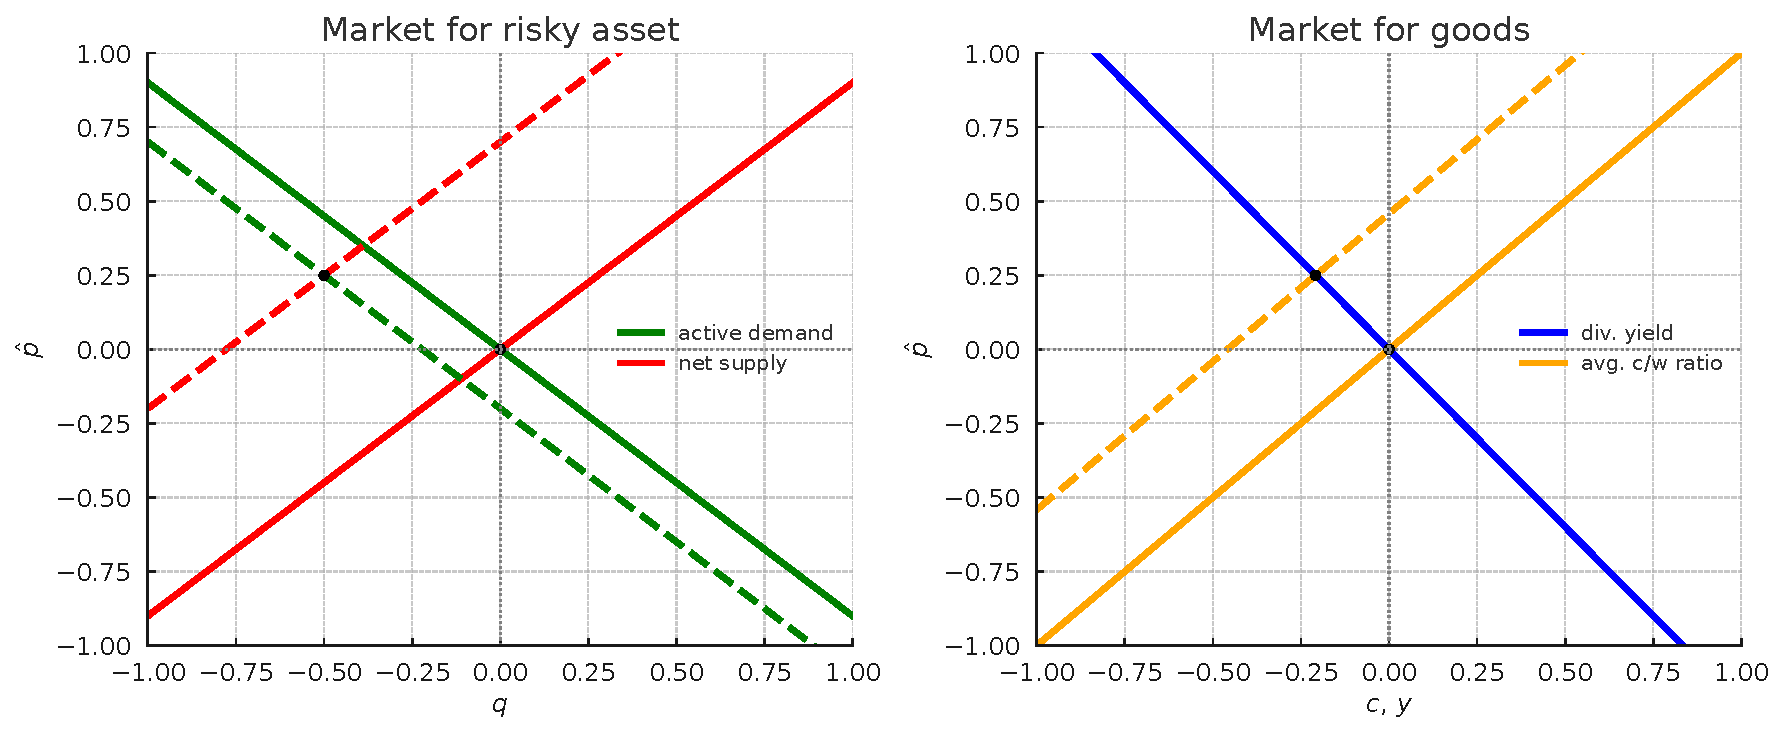
\includegraphics[width=0.95\linewidth]{figures/mkt_equilibrium2.pdf}
    \vspace{2mm}
    \caption{Equilibrium with inefficient risk allocation: risky asset (left) and goods (right) markets.}
    \label{fig:mkt_equilibrium2}
\end{figure}

Figure~\ref{fig:mkt_equilibrium2} illustrates the effects of portfolio flows when passive investors are initially underexposed to risk, i.e., $\overline{\alpha}_{p,t}<1$. An inflow into the risky asset shifts both the net supply curve (left panel) and the average consumption-wealth ratio schedule (right panel) leftward. The interest rate adjusts so that active demand meets net supply at the goods market clearing price. In this case, portfolio flows have a positive price impact and the aggregate elasticity is \textit{finite}.  

\begin{prop}[Aggregate elasticity: inefficient passive demand]\label{prop:elasticity_passive_demand}
Without preference heterogeneity or leverage constraints, the inverse aggregate elasticity is
\begin{equation}\label{eq:elasticity_passive_demand}
    \varepsilon_{M,t}^{-1}
    \;=\;
    -\,(\chi_{p}+y^\star)^{-1}\,\frac{\partial \chi_{0,t}}{\partial f_t}
    \;=\;
    \left(1-\psi^{-1}\right)\frac{\gamma \|\sigma\|^{2}}{y^\star}
    \frac{1-\overline{\alpha}_{p,t}}{x_{a,t}}
    \;+\;\mathcal{O}\!\left(\epsilon^{2}\right),
\end{equation}
where $x_{a,t}=1-x_{0,t}$ is the wealth share of active investors and $y^\star=1/p^\star$ is the dividend-price ratio in the benchmark economy.
\end{prop}

Proposition~\ref{prop:elasticity_passive_demand} shows that, unlike in \citet{gabaix2020search}, the risky-asset elasticities $\zeta_p$ and $\zeta_r$ are not the direct drivers of aggregate elasticity. Because the demand system is recursive (interest rates only enters the risky asset demand) the overall price impact is governed instead by how portfolio flows impact the consumption-wealth ratio. %In other words, aggregate elasticity reflects changes in savings behavior rather than the direct slope of risky asset demand.


The macro elasticity is finite whenever $\overline{\alpha}_{p,t}\neq 1$ and $\psi\neq 1$. In the unit EIS case, the price-dividend ratio is pinned down by the subjective discount rate, so portfolio flows generate offsetting movements in the risk premium and the risk-free rate. With efficient risk allocation ($\overline{\alpha}_{p,t}=1$), there is again no price impact.  

The price impact is positive when $\psi>1$ and $\overline{\alpha}_{p,t}<1$: interest rate adjustments no longer fully offset the risk premium response, so the latter dominates. This mirrors representative agent models in which uncertainty shocks affect prices only when $\psi>1$ \citep[e.g.,][]{bansal2004risks}.  

The state-global perturbation analysis also makes clear that elasticity is state dependent. Figure~\ref{Fig:elasticity_passive-demand} plots the price impact as a function of active investors' wealth for different passive-share levels.  Price impact rises when active investors are under capitalized, reflecting their limited risk-bearing capacity, and when the passive share deviates further from its efficient level. In the extreme case where passive investors hold no equities ($\overline{\alpha}_{p,t}=0$), we recover a version of \citet{basak1998equilibrium} in which price impact is maximized.  


\begin{figure}[!t]
    \centering
    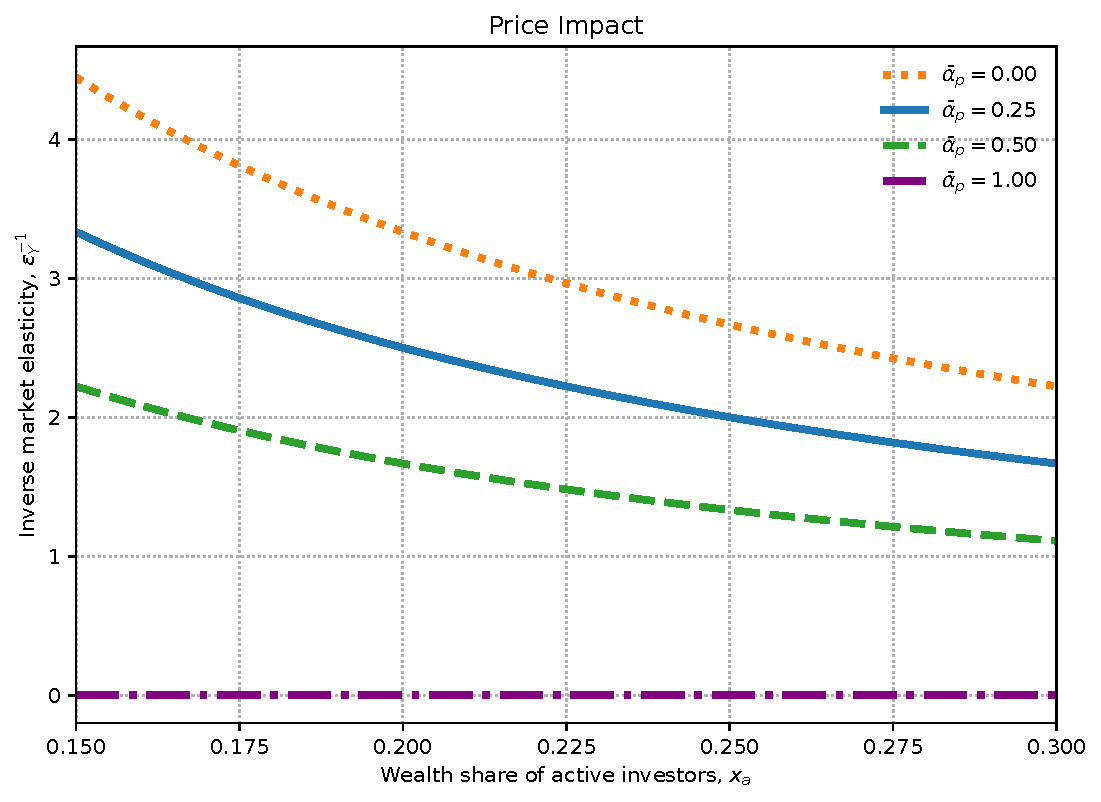
\includegraphics[width=0.6\textwidth]{./figures/price_impact_passive2.pdf}
    \vspace{2mm}
    \caption{Price impact: inefficient passive demand.}
    \label{Fig:elasticity_passive-demand}
\end{figure}

\subsection{Preference heterogeneity and leverage constraints}

We now reintroduce preference heterogeneity and leverage constraints into the model. These features shift the conditions under which passive investors’ portfolios are efficient and therefore alter the aggregate market elasticity. The next proposition provides the main result.

\begin{prop}[Aggregate elasticity: heterogeneity and leverage constraints]\label{prop_elasticity_pref_heterog}
The inverse aggregate market elasticity is
\begin{equation}\label{eq:elasticity_pref_heterog}
    \varepsilon_{M,t}^{-1}
    \;=\;
    \bigl(1-\psi^{-1}\bigr)\,
    \frac{\gamma\,\|\sigma\|^{2}}{y^\star}\,
    \frac{\overline{\alpha}_{p,t}^{\mathrm{opt}}-\overline{\alpha}_{p,t}}{x_{a,t}-x_{c,t}}\,
    \bigl(1-x_{c,t}\bigr)
    \;+\;\mathcal{O}\!\left(\epsilon^{2}\right),
\end{equation}
where $x_{c,t}$ is the wealth share of constrained active investors and the passive investors’ optimal portfolio share is
\begin{equation}\label{eq:optimal_alpha_p}
    \overline{\alpha}_{p,t}^{\mathrm{opt}}
    \;=\;
    1
    \;-\;
    \frac{x_{a,t}-x_{c,t}}{1-x_{c,t}}\,
    \frac{\gamma_{0}-\mathbb{E}^{u}_{t}[\gamma_{j}]}{\gamma}
    \;-\;
    \frac{x_{c,t}}{1-x_{c,t}}
    \Bigl(\frac{\overline{\sigma}}{\|\sigma\|}-1\Bigr),
\end{equation}
with $x_{u,t}\equiv x_{a,t}-x_{c,t}$ the wealth share of unconstrained active investors and 
\[
    \mathbb{E}^{u}_{t}[\gamma_{j}]
    \;\equiv\;
    \sum_{j\in\mathcal{J}^{u}}\frac{x_{j,t}}{x_{u,t}}\,\gamma_{j}.
\]
\end{prop}

Proposition~\ref{prop_elasticity_pref_heterog} characterizes aggregate market elasticity in the full model. As in the frictionless benchmark, the market remains infinitely elastic when passive investors hold their optimal portfolio share, $\overline{\alpha}_{p,t}=\overline{\alpha}_{p,t}^{\mathrm{opt}}$. 
The optimal portfolio share corresponds to the value of $\overline{\alpha}_{p,t}$ such that the passive investor would have no incentive to change their portfolio. 
Under homogeneous preferences ($\gamma_j=\gamma$) and slack leverage constraints ($x_{c,t}=0$), this condition reduces to $\overline{\alpha}_{p,t}=1$. More generally, preference heterogeneity and binding leverage constraints shift the efficient passive share away from unity, with its level determined by the wealth distribution and the relative risk aversion of different investor types.

\paragraph{Preference heterogeneity.}
With slack leverage constraints ($x_{c,t}=0$), \eqref{eq:optimal_alpha_p} simplifies to
\[
\overline{\alpha}_{p,t}^{\mathrm{opt}}
= 1 - x_{a,t}\,\frac{\gamma_0-\mathbb{E}^u_t[\gamma_j]}{\gamma},
\]
so, unlike the homogeneous preference case, the efficient passive share $\overline{\alpha}_{p,t}^{\mathrm{opt}}$ differs from unity whenever $\gamma_0 \neq \mathbb{E}^u_t[\gamma_j]$. The inverse elasticity in \eqref{eq:elasticity_pref_heterog} becomes
\[
\varepsilon_{M,t}^{-1}
= \bigl(1-\psi^{-1}\bigr)\,\frac{\gamma\|\sigma\|^2}{y^\star}\,
\frac{\overline{\alpha}_{p,t}^{\mathrm{opt}}-\overline{\alpha}_{p,t}}{x_{a,t}}
\;+\;\mathcal{O}(\epsilon^2).
\]

Optimal risk sharing implies that when passive investors are more risk averse than the average unconstrained active ($\gamma_0>\mathbb{E}^u_t[\gamma_j]$),
\[
\frac{\partial \overline{\alpha}_{p,t}^{\mathrm{opt}}}{\partial x_{a,t}}
= -\,\frac{\gamma_0-\mathbb{E}^u_t[\gamma_j]}{\gamma} < 0,
\]
so the efficient passive equity share rises as the active wealth share falls, typically after adverse aggregate shocks that erode active wealth that is more exposed to risk. If passive investors do not rebalance in such episodes, market inelasticity increases because $x_{a,t}$ declines (reducing risk-bearing capacity) while the gap $\overline{\alpha}_{p,t}^{\mathrm{opt}}-\overline{\alpha}_{p,t}$ widens (moving the economy farther from the efficient allocation). Consequently, price impact rises as $x_{a,t}$ falls, as shown in the left panel (a) of Figure~\ref{fig:price_impact_comparison}: the heterogeneous- and homogeneous-preference curves coincide at $x_{a}=0.20$, but only the former steepens markedly as $x_a$ declines.


\begin{figure}[t!]
    \centering
    \begin{subfigure}[t]{0.48\textwidth}
        \centering
        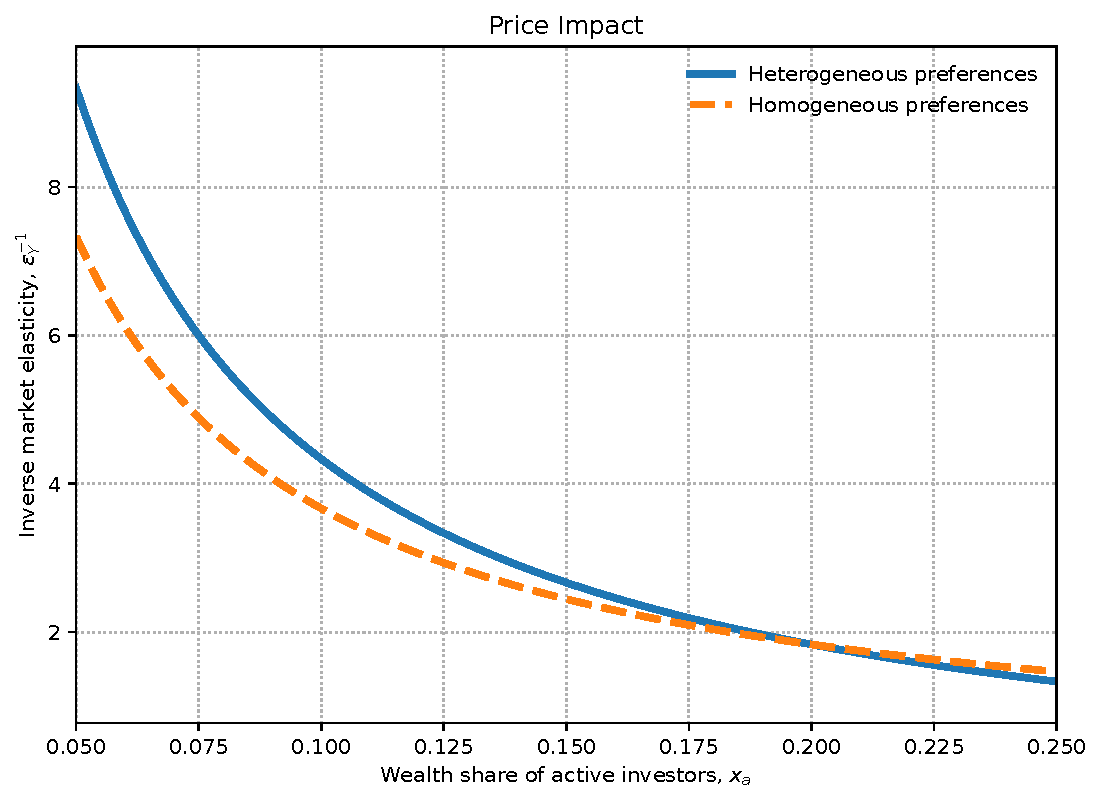
\includegraphics[width=\linewidth]{figures/price_impact_heterogeneity1.pdf}
        \caption{Homogeneous vs. heterogeneous preferences}
        \label{fig:impact_het_vs_hom}
    \end{subfigure}\hfill
    \begin{subfigure}[t]{0.48\textwidth}
        \centering
        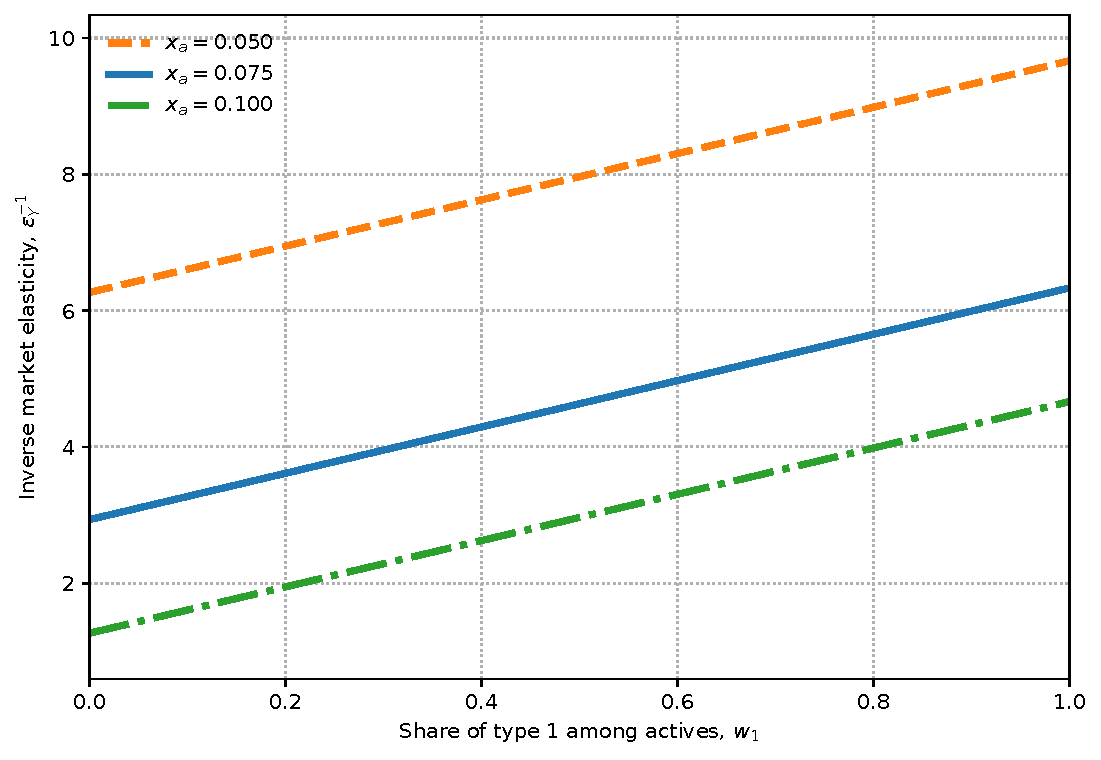
\includegraphics[width=\linewidth]{figures/price_impact_heterogeneity2.pdf}
        \caption{Role of wealth distribution of active investors}
        \label{fig:impact_vs_w1_by_alphap}
    \end{subfigure}
    \vspace{2mm}
    \caption{\textbf{Price impact comparisons.}\\ Panel (a) compares heterogeneous and homogeneous preferences. Panel (b) shows the sensitivity of the price impact to wealth distribution among active investors when $J=2$ for different passive portfolio shares.}
    \label{fig:price_impact_comparison}
\end{figure}

Panel (b) of Figure~\ref{fig:price_impact_comparison} shows how the distribution of wealth across active investors shapes price impact. With two active types ($J=2$) and $\gamma_1>\gamma_2$, the average risk active aversion is
\[
\mathbb{E}^u_t[\gamma_j] \;=\; w_{1,t}\gamma_1 + \bigl(1-w_{1,t}\bigr)\gamma_2,
\qquad
w_{1,t}\equiv \frac{x_{1,t}}{x_{a,t}}.
\]
When leverage constraints are slack ($x_{c,t}=0$), the efficient passive share satisfies
\(
\overline{\alpha}_{p,t}^{\mathrm{opt}}
= 1 - x_{a,t}\,(\gamma_0-\mathbb{E}^u_t[\gamma_j])/\gamma,
\)
so holding $x_{a,t}$ fixed,
\[
\frac{\partial\,\overline{\alpha}_{p,t}^{\mathrm{opt}}}{\partial w_{1,t}}
= \frac{x_{a,t}}{\gamma}\,(\gamma_1-\gamma_2) \;>\; 0.
\]
Thus, as the wealth share of the more risk averse active type rises, $\mathbb{E}^u_t[\gamma_j]$ increases and the passive sector should optimally hold more of the risky asset. If the passive portfolio is not adjusted, the deviation $\overline{\alpha}_{p,t}^{\mathrm{opt}}-\overline{\alpha}_{p,t}$ widens, worsening risk allocation and raising price impact, consistent with the upward shift in the panel~(b) of Figure~\ref{fig:price_impact_comparison}.



\paragraph{Leverage constraints.}
When some active investors are constrained ($x_{c,t}>0$), the marginal investors are the \emph{unconstrained} active agents, and their risk-bearing capacity,
\[
x_{u,t}\;\equiv\;x_{a,t}-x_{c,t},
\]
becomes the key determinant of price impact. The panel (a) of Figure~\ref{fig:price_impact_leverage_constraints} plots price impact against the active wealth share $x_{a,t}=1-x_{0,t}$, with and without binding constraints. To isolate the role of constraints, we set $\gamma_0=\mathbb{E}_t^{u}[\gamma_j]$, removing pure preference heterogeneity effects. As $x_{a,t}$ declines, e.g., after a negative aggregate shock when $\overline{\alpha}_{p,t}<1$, price impact rises more sharply under binding constraints because $x_{u,t}$ shrinks and the risk-bearing capacity of marginal investors is depleted. Panel (b) holds $x_{a,t}$ fixed and varies the constrained share $x_{c,t}$. The price impact increases monotonically with $x_{c,t}$. This is intuitive: price impact is larger when a larger share of active investors is constrained.

\begin{figure}[t!]
    \centering
    \begin{subfigure}[t]{0.48\textwidth}
        \centering
        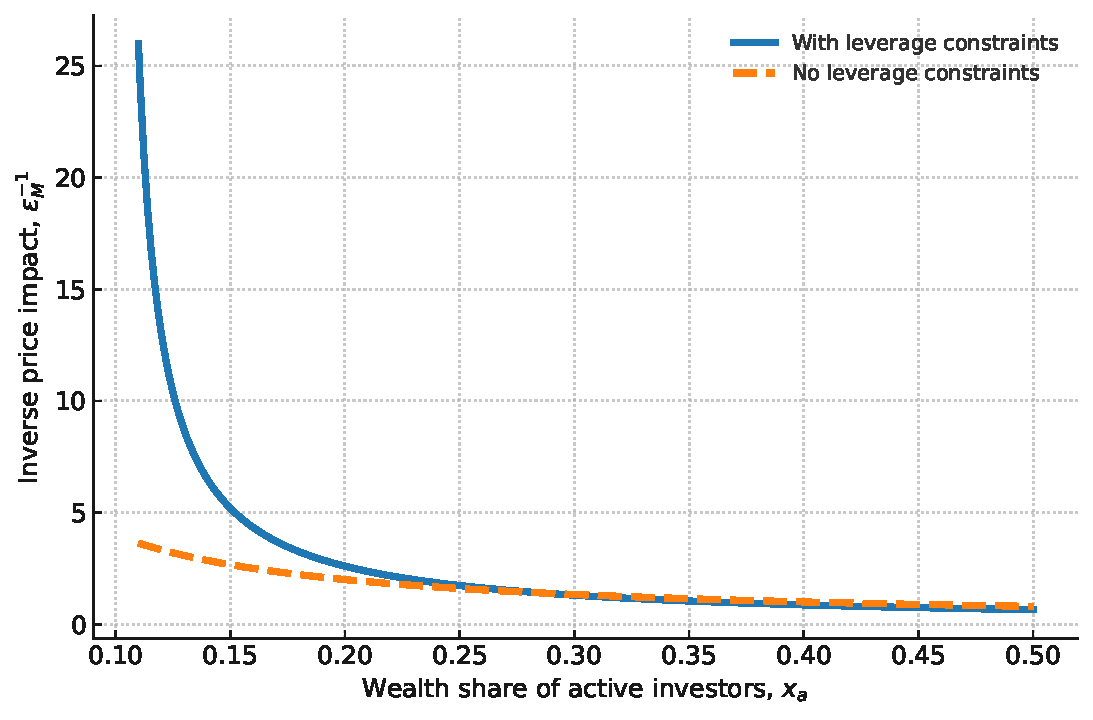
\includegraphics[width=\linewidth]{figures/price_impact_lev_constraints1.pdf}
        \caption{Role of leverage constraints \emph{(assumes $x_{c,t}=0.10$)}}
    \end{subfigure}\hfill
    \begin{subfigure}[t]{0.48\textwidth}
        \centering
        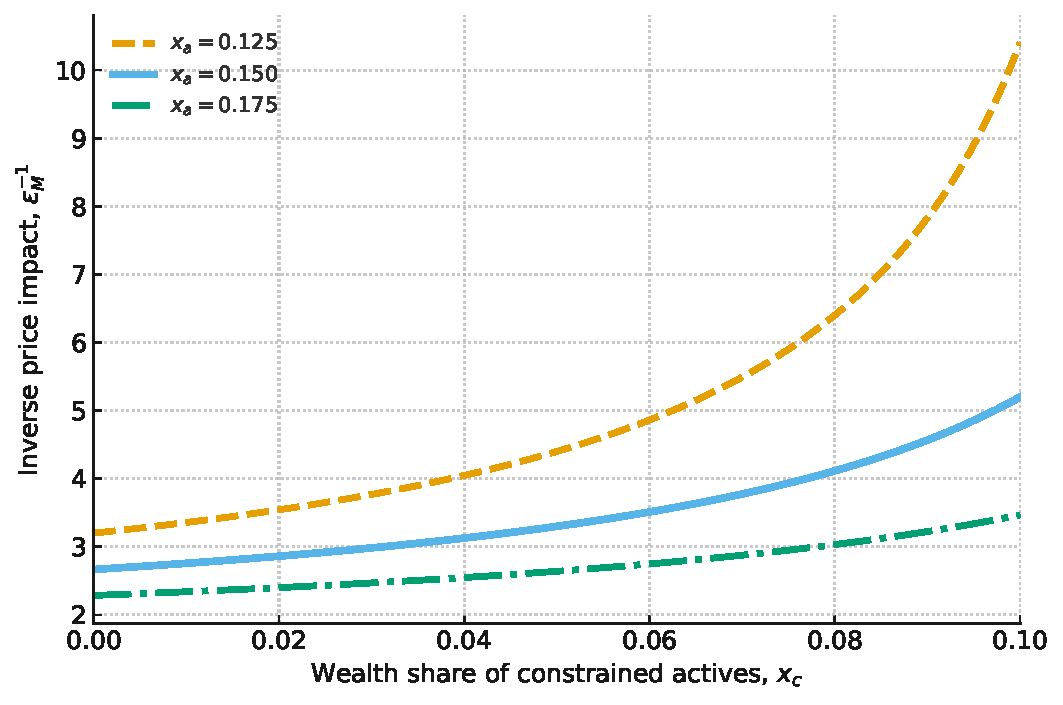
\includegraphics[width=\linewidth]{figures/price_impact_lev_constraints2.pdf}
        \caption{Varying the wealth share of constrained actives, $x_{c,t}$}
    \end{subfigure}
    \vspace{2mm}
    \caption{Price impact under leverage constraints. Panel (a) compares the cases with and without leverage constraints (holding $x_{c,t}=0.10$). Panel (b) plots the price impact as a function of $x_{c,t}$ for different values of $x_{a,t}$.}
    \label{fig:price_impact_leverage_constraints}
\end{figure}

\paragraph{Taking stock.}
Proposition~\ref{prop_elasticity_pref_heterog} clarifies the main determinants of aggregate market elasticity. The elasticity is \emph{finite} only when risk is misallocated: small portfolio flows around the frictionless allocation have no first-order price impact. Preference heterogeneity amplifies price impact in downturns because, as the active wealth share falls, the efficient passive share rises, widening the gap between efficient and actual portfolios. Binding leverage constraints further increase price impact by shrinking the marginal (unconstrained) risk-bearing capacity, $x_{u,t}$. Taken together, these forces imply rich state dependence of aggregate elasticity in economies with heterogeneous investors and financial frictions.


\section{Quantitative Implications}\label{sec:quantitative}

We now evaluate the quantitative implications of the dynamic model of Section~\ref{sec:model}.
The exercise has two goals.
The first is to ask whether a calibration disciplined by U.S. data on sectoral portfolio holdings and passive equity flows can simultaneously deliver an empirically plausible price impact and the standard asset-pricing moments.
The second is to quantify how much of the variation in return volatility, return predictability, and the variance of the price--dividend ratio is attributable to how portfolio flows interact with preference heterogeneity, leverage constraints, and passive-sector risk misallocation.
We do the latter by comparing the baseline economy to a set of counterfactuals that turn off these frictions one at a time.

We solve the full dynamic system numerically using the neural-network method of \citet{duarte2024machine}, which accommodates the four state variables: passive demand, the dividend share, and the wealth shares of the constrained and unconstrained active sectors.
Appendix~\ref{app:numerical} describes the numerical procedure in detail.

\subsection{Calibration}\label{sec:calibration}

We aggregate Flow of Funds (FoF) sectors into three ultimate sectors: a passive sector, a constrained active sector, and an unconstrained active sector.\footnote{We follow the aggregation in \citet{koijen2024investors}.
Appendix~\ref{app:fof_aggregation} describes the sector mapping and the treatment of pass-through vehicles in detail.}
The passive sector is modeled as an exogenous CIR process for the portfolio share $\overline{\alpha}_{p,t}$ in Equation~\eqref{eq:alpha_p_process}.
The two active sectors differ both in risk aversion and in whether they are subject to the leverage constraint.
Table~\ref{tab:calib} reports the calibrated parameter values, and the next subsection describes the moments used to discipline them.

Figure~\ref{fig:facts-vol-flow} motivates two of the calibration targets.
The left panel plots quarterly aggregate equity flows, scaled by lagged market capitalization as in Appendix~D3 of \citet{gabaix2020search}, together with realized return volatility.
The right panel reports the ``volatility multiplier,'' defined as the ratio of realized return volatility to quarterly flows.
The multiplier is a reduced-form analog of the price impact that our calibration aims to reproduce.

\begin{figure}[!t]
    \centering
    \subfloat{\resizebox{0.49\textwidth}{!}{% Created by tikzDevice version 0.12.4 on 2023-11-04 17:00:14
% !TEX encoding = UTF-8 Unicode
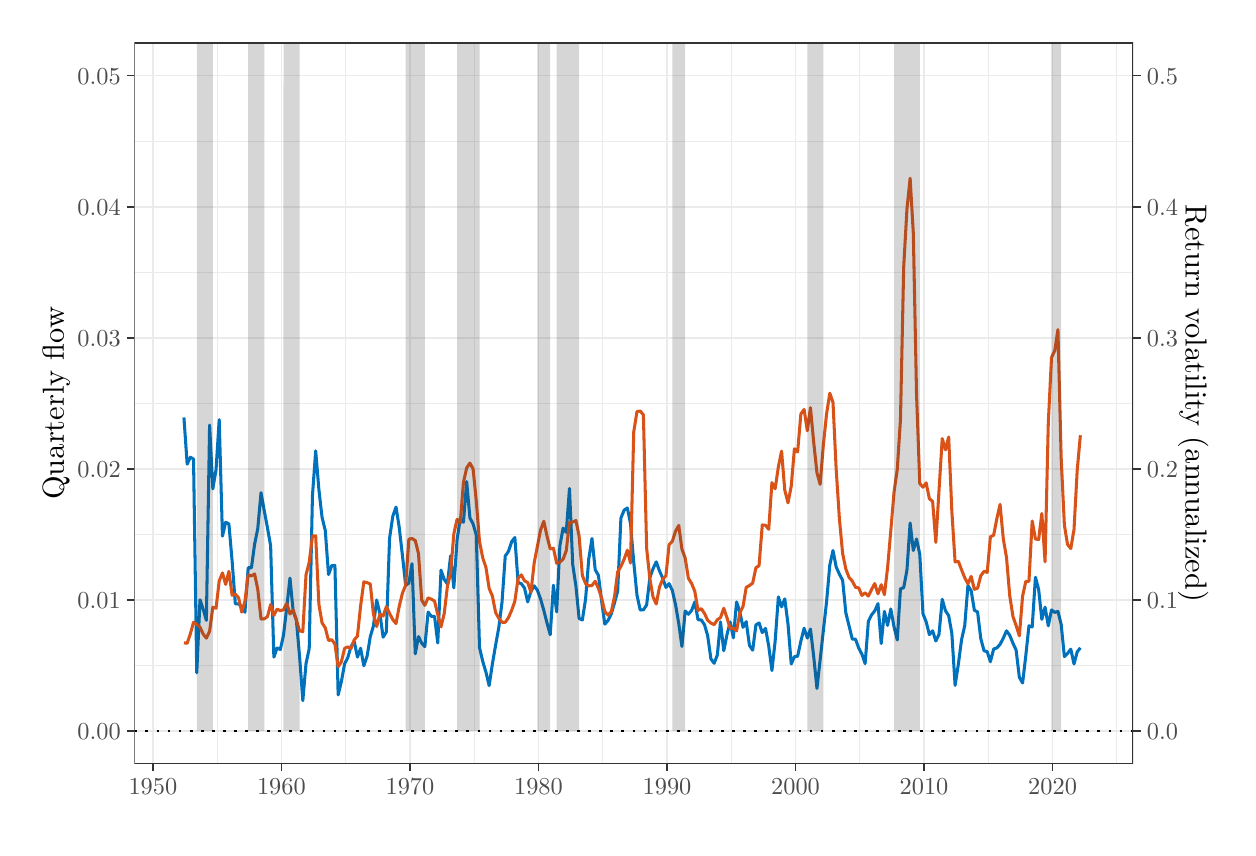
\begin{tikzpicture}[x=1pt,y=1pt]
\definecolor{fillColor}{RGB}{255,255,255}
\path[use as bounding box,fill=fillColor,fill opacity=0.00] (0,0) rectangle (433.62,289.08);
\begin{scope}
\path[clip] (  0.00,  0.00) rectangle (433.62,289.08);
\definecolor{drawColor}{RGB}{255,255,255}
\definecolor{fillColor}{RGB}{255,255,255}

\path[draw=drawColor,line width= 0.6pt,line join=round,line cap=round,fill=fillColor] (  0.00,  0.00) rectangle (433.62,289.08);
\end{scope}
\begin{scope}
\path[clip] ( 38.56, 23.11) rectangle (399.46,283.58);
\definecolor{fillColor}{RGB}{255,255,255}

\path[fill=fillColor] ( 38.56, 23.11) rectangle (399.46,283.58);
\definecolor{drawColor}{gray}{0.92}

\path[draw=drawColor,line width= 0.3pt,line join=round] ( 38.56, 58.63) --
	(399.46, 58.63);

\path[draw=drawColor,line width= 0.3pt,line join=round] ( 38.56,105.99) --
	(399.46,105.99);

\path[draw=drawColor,line width= 0.3pt,line join=round] ( 38.56,153.34) --
	(399.46,153.34);

\path[draw=drawColor,line width= 0.3pt,line join=round] ( 38.56,200.70) --
	(399.46,200.70);

\path[draw=drawColor,line width= 0.3pt,line join=round] ( 38.56,248.06) --
	(399.46,248.06);

\path[draw=drawColor,line width= 0.3pt,line join=round] ( 68.46, 23.11) --
	( 68.46,283.58);

\path[draw=drawColor,line width= 0.3pt,line join=round] (114.91, 23.11) --
	(114.91,283.58);

\path[draw=drawColor,line width= 0.3pt,line join=round] (161.35, 23.11) --
	(161.35,283.58);

\path[draw=drawColor,line width= 0.3pt,line join=round] (207.79, 23.11) --
	(207.79,283.58);

\path[draw=drawColor,line width= 0.3pt,line join=round] (254.24, 23.11) --
	(254.24,283.58);

\path[draw=drawColor,line width= 0.3pt,line join=round] (300.68, 23.11) --
	(300.68,283.58);

\path[draw=drawColor,line width= 0.3pt,line join=round] (347.13, 23.11) --
	(347.13,283.58);

\path[draw=drawColor,line width= 0.3pt,line join=round] (393.57, 23.11) --
	(393.57,283.58);

\path[draw=drawColor,line width= 0.6pt,line join=round] ( 38.56, 34.95) --
	(399.46, 34.95);

\path[draw=drawColor,line width= 0.6pt,line join=round] ( 38.56, 82.31) --
	(399.46, 82.31);

\path[draw=drawColor,line width= 0.6pt,line join=round] ( 38.56,129.67) --
	(399.46,129.67);

\path[draw=drawColor,line width= 0.6pt,line join=round] ( 38.56,177.02) --
	(399.46,177.02);

\path[draw=drawColor,line width= 0.6pt,line join=round] ( 38.56,224.38) --
	(399.46,224.38);

\path[draw=drawColor,line width= 0.6pt,line join=round] ( 38.56,271.74) --
	(399.46,271.74);

\path[draw=drawColor,line width= 0.6pt,line join=round] ( 45.24, 23.11) --
	( 45.24,283.58);

\path[draw=drawColor,line width= 0.6pt,line join=round] ( 91.68, 23.11) --
	( 91.68,283.58);

\path[draw=drawColor,line width= 0.6pt,line join=round] (138.13, 23.11) --
	(138.13,283.58);

\path[draw=drawColor,line width= 0.6pt,line join=round] (184.57, 23.11) --
	(184.57,283.58);

\path[draw=drawColor,line width= 0.6pt,line join=round] (231.02, 23.11) --
	(231.02,283.58);

\path[draw=drawColor,line width= 0.6pt,line join=round] (277.46, 23.11) --
	(277.46,283.58);

\path[draw=drawColor,line width= 0.6pt,line join=round] (323.91, 23.11) --
	(323.91,283.58);

\path[draw=drawColor,line width= 0.6pt,line join=round] (370.35, 23.11) --
	(370.35,283.58);
\definecolor{drawColor}{RGB}{0,114,189}

\path[draw=drawColor,line width= 1.1pt,line join=round] ( 56.46,148.23) --
	( 57.63,131.35) --
	( 58.78,133.87) --
	( 59.93,133.20) --
	( 61.10, 55.94) --
	( 62.27, 82.35) --
	( 63.43, 78.92) --
	( 64.57, 74.89) --
	( 65.74,145.46) --
	( 66.91,122.40) --
	( 68.07,129.42) --
	( 69.21,147.43) --
	( 70.38,105.35) --
	( 71.55,110.38) --
	( 72.71,109.76) --
	( 73.87, 96.40) --
	( 75.04, 80.86) --
	( 76.20, 80.88) --
	( 77.36, 79.88) --
	( 78.51, 77.82) --
	( 79.68, 93.93) --
	( 80.85, 93.90) --
	( 82.00,102.42) --
	( 83.15,108.14) --
	( 84.32,121.04) --
	( 85.49,114.52) --
	( 86.64,108.37) --
	( 87.79,101.91) --
	( 88.96, 61.63) --
	( 90.13, 64.95) --
	( 91.29, 64.36) --
	( 92.44, 69.56) --
	( 93.61, 79.49) --
	( 94.78, 90.18) --
	( 95.94, 78.14) --
	( 97.08, 75.12) --
	( 98.25, 61.92) --
	( 99.42, 45.90) --
	(100.58, 59.30) --
	(101.73, 64.67) --
	(102.90,119.95) --
	(104.07,136.18) --
	(105.22,122.28) --
	(106.37,112.15) --
	(107.54,107.36) --
	(108.71, 91.45) --
	(109.86, 94.67) --
	(111.02, 94.74) --
	(112.19, 47.96) --
	(113.36, 52.82) --
	(114.52, 59.22) --
	(115.66, 61.39) --
	(116.83, 65.47) --
	(118.00, 67.32) --
	(119.16, 61.64) --
	(120.30, 64.84) --
	(121.47, 58.49) --
	(122.64, 61.94) --
	(123.80, 68.99) --
	(124.94, 72.90) --
	(126.11, 82.27) --
	(127.28, 77.37) --
	(128.44, 68.83) --
	(129.60, 70.71) --
	(130.77,104.58) --
	(131.94,112.55) --
	(133.10,115.85) --
	(134.24,108.68) --
	(135.41, 98.46) --
	(136.58, 87.58) --
	(137.74, 88.39) --
	(138.88, 95.39) --
	(140.05, 62.80) --
	(141.22, 69.07) --
	(142.38, 66.67) --
	(143.52, 65.38) --
	(144.69, 77.91) --
	(145.86, 76.38) --
	(147.02, 76.35) --
	(148.18, 66.75) --
	(149.35, 93.06) --
	(150.52, 89.72) --
	(151.67, 88.05) --
	(152.82, 98.25) --
	(153.99, 86.66) --
	(155.16,104.07) --
	(156.31,111.69) --
	(157.46,110.35) --
	(158.63,125.07) --
	(159.80,111.97) --
	(160.96,109.72) --
	(162.10,105.75) --
	(163.27, 65.08) --
	(164.44, 60.06) --
	(165.60, 56.18) --
	(166.75, 51.32) --
	(167.92, 59.16) --
	(169.09, 65.97) --
	(170.25, 72.39) --
	(171.40, 81.43) --
	(172.57, 98.18) --
	(173.73, 99.82) --
	(174.89,103.34) --
	(176.04,104.86) --
	(177.21, 88.53) --
	(178.38, 88.19) --
	(179.53, 86.58) --
	(180.68, 81.58) --
	(181.85, 85.38) --
	(183.02, 87.39) --
	(184.17, 85.81) --
	(185.33, 82.66) --
	(186.50, 78.55) --
	(187.67, 73.90) --
	(188.83, 69.71) --
	(189.97, 87.62) --
	(191.14, 77.98) --
	(192.31,101.82) --
	(193.47,108.25) --
	(194.61,106.69) --
	(195.78,122.58) --
	(196.95, 95.08) --
	(198.11, 87.28) --
	(199.26, 75.61) --
	(200.43, 75.03) --
	(201.60, 82.62) --
	(202.75, 97.16) --
	(203.91,104.49) --
	(205.08, 93.21) --
	(206.25, 91.12) --
	(207.41, 81.73) --
	(208.55, 73.54) --
	(209.72, 74.87) --
	(210.89, 77.29) --
	(212.05, 81.20) --
	(213.19, 85.43) --
	(214.36,111.86) --
	(215.53,114.75) --
	(216.69,115.53) --
	(217.83,109.83) --
	(219.00, 95.94) --
	(220.17, 84.02) --
	(221.33, 78.66) --
	(222.49, 78.71) --
	(223.66, 80.48) --
	(224.83, 90.41) --
	(225.98, 93.59) --
	(227.13, 96.06) --
	(228.30, 92.78) --
	(229.47, 90.17) --
	(230.63, 86.82) --
	(231.77, 88.18) --
	(232.94, 85.72) --
	(234.11, 80.54) --
	(235.27, 73.75) --
	(236.41, 65.47) --
	(237.58, 78.29) --
	(238.75, 77.12) --
	(239.91, 78.51) --
	(241.06, 81.54) --
	(242.23, 75.15) --
	(243.40, 75.05) --
	(244.56, 73.36) --
	(245.71, 69.40) --
	(246.88, 61.00) --
	(248.05, 59.40) --
	(249.20, 62.36) --
	(250.35, 74.36) --
	(251.52, 63.92) --
	(252.69, 69.71) --
	(253.84, 74.34) --
	(254.99, 68.59) --
	(256.16, 81.58) --
	(257.33, 77.98) --
	(258.49, 72.40) --
	(259.64, 74.44) --
	(260.81, 65.85) --
	(261.98, 64.13) --
	(263.14, 73.26) --
	(264.28, 73.98) --
	(265.45, 70.49) --
	(266.62, 72.03) --
	(267.78, 65.60) --
	(268.93, 56.78) --
	(270.10, 67.42) --
	(271.26, 83.40) --
	(272.42, 79.82) --
	(273.57, 82.68) --
	(274.74, 73.61) --
	(275.91, 59.14) --
	(277.06, 61.79) --
	(278.22, 61.96) --
	(279.39, 67.39) --
	(280.56, 72.08) --
	(281.72, 68.52) --
	(282.86, 71.76) --
	(284.03, 61.85) --
	(285.20, 50.31) --
	(286.36, 60.66) --
	(287.50, 71.10) --
	(288.67, 81.53) --
	(289.84, 94.91) --
	(291.00,100.15) --
	(292.14, 94.25) --
	(293.31, 91.60) --
	(294.48, 89.41) --
	(295.64, 77.63) --
	(296.80, 72.95) --
	(297.97, 68.14) --
	(299.14, 68.10) --
	(300.30, 64.88) --
	(301.44, 62.72) --
	(302.61, 59.25) --
	(303.78, 74.55) --
	(304.94, 76.89) --
	(306.08, 78.32) --
	(307.25, 80.95) --
	(308.42, 66.52) --
	(309.58, 78.17) --
	(310.72, 73.09) --
	(311.89, 79.03) --
	(313.06, 72.53) --
	(314.22, 67.82) --
	(315.38, 86.32) --
	(316.55, 86.73) --
	(317.72, 93.05) --
	(318.87,110.10) --
	(320.02,100.16) --
	(321.19,104.32) --
	(322.36, 98.80) --
	(323.51, 77.33) --
	(324.66, 74.39) --
	(325.83, 69.74) --
	(327.00, 71.15) --
	(328.16, 67.46) --
	(329.30, 69.85) --
	(330.47, 82.54) --
	(331.64, 78.38) --
	(332.80, 76.60) --
	(333.95, 70.19) --
	(335.12, 51.40) --
	(336.29, 59.02) --
	(337.45, 67.88) --
	(338.60, 72.98) --
	(339.76, 87.52) --
	(340.93, 85.63) --
	(342.09, 78.53) --
	(343.24, 77.98) --
	(344.41, 68.27) --
	(345.58, 63.96) --
	(346.73, 63.57) --
	(347.88, 59.95) --
	(349.05, 64.56) --
	(350.22, 64.98) --
	(351.37, 66.23) --
	(352.53, 68.46) --
	(353.70, 71.13) --
	(354.87, 69.50) --
	(356.03, 66.65) --
	(357.17, 64.18) --
	(358.34, 54.32) --
	(359.51, 52.28) --
	(360.67, 62.19) --
	(361.81, 72.94) --
	(362.98, 72.51) --
	(364.15, 90.49) --
	(365.31, 86.11) --
	(366.46, 75.25) --
	(367.63, 79.68) --
	(368.80, 72.94) --
	(369.95, 78.69) --
	(371.11, 77.80) --
	(372.28, 78.14) --
	(373.45, 73.51) --
	(374.61, 61.79) --
	(375.75, 62.97) --
	(376.92, 64.51) --
	(378.09, 59.15) --
	(379.25, 63.53) --
	(380.39, 65.00);
\definecolor{drawColor}{RGB}{217,83,25}

\path[draw=drawColor,line width= 1.1pt,line join=round] ( 56.46, 66.79) --
	( 57.63, 66.63) --
	( 58.78, 70.01) --
	( 59.93, 74.24) --
	( 61.10, 73.46) --
	( 62.27, 72.45) --
	( 63.43, 69.92) --
	( 64.57, 68.49) --
	( 65.74, 70.98) --
	( 66.91, 79.67) --
	( 68.07, 79.29) --
	( 69.21, 89.14) --
	( 70.38, 92.05) --
	( 71.55, 87.89) --
	( 72.71, 92.64) --
	( 73.87, 84.00) --
	( 75.04, 84.38) --
	( 76.20, 83.09) --
	( 77.36, 77.90) --
	( 78.51, 81.82) --
	( 79.68, 91.35) --
	( 80.85, 90.96) --
	( 82.00, 91.70) --
	( 83.15, 86.06) --
	( 84.32, 75.39) --
	( 85.49, 75.45) --
	( 86.64, 76.25) --
	( 87.79, 80.63) --
	( 88.96, 76.66) --
	( 90.13, 78.98) --
	( 91.29, 78.40) --
	( 92.44, 78.75) --
	( 93.61, 81.06) --
	( 94.78, 77.21) --
	( 95.94, 78.67) --
	( 97.08, 74.98) --
	( 98.25, 71.08) --
	( 99.42, 70.85) --
	(100.58, 91.38) --
	(101.73, 95.84) --
	(102.90,105.40) --
	(104.07,105.47) --
	(105.22, 80.76) --
	(106.37, 74.04) --
	(107.54, 72.19) --
	(108.71, 67.64) --
	(109.86, 67.92) --
	(111.02, 66.37) --
	(112.19, 58.11) --
	(113.36, 59.95) --
	(114.52, 64.81) --
	(115.66, 65.33) --
	(116.83, 64.75) --
	(118.00, 67.89) --
	(119.16, 69.21) --
	(120.30, 80.08) --
	(121.47, 88.83) --
	(122.64, 88.53) --
	(123.80, 88.06) --
	(124.94, 77.14) --
	(126.11, 72.68) --
	(127.28, 77.15) --
	(128.44, 76.49) --
	(129.60, 79.88) --
	(130.77, 77.45) --
	(131.94, 75.16) --
	(133.10, 73.75) --
	(134.24, 79.88) --
	(135.41, 84.72) --
	(136.58, 87.65) --
	(137.74,104.26) --
	(138.88,104.48) --
	(140.05,103.77) --
	(141.22, 99.06) --
	(142.38, 82.25) --
	(143.52, 80.33) --
	(144.69, 83.03) --
	(145.86, 82.59) --
	(147.02, 81.88) --
	(148.18, 77.04) --
	(149.35, 72.54) --
	(150.52, 77.41) --
	(151.67, 87.21) --
	(152.82, 91.97) --
	(153.99,106.16) --
	(155.16,111.43) --
	(156.31,110.05) --
	(157.46,124.74) --
	(158.63,130.00) --
	(159.80,131.73) --
	(160.96,129.62) --
	(162.10,118.01) --
	(163.27,103.44) --
	(164.44, 97.48) --
	(165.60, 93.99) --
	(166.75, 86.47) --
	(167.92, 83.69) --
	(169.09, 77.73) --
	(170.25, 75.65) --
	(171.40, 74.24) --
	(172.57, 74.19) --
	(173.73, 75.89) --
	(174.89, 78.55) --
	(176.04, 81.81) --
	(177.21, 90.12) --
	(178.38, 91.36) --
	(179.53, 89.21) --
	(180.68, 88.59) --
	(181.85, 85.09) --
	(183.02, 95.64) --
	(184.17,101.64) --
	(185.33,107.56) --
	(186.50,110.74) --
	(187.67,105.31) --
	(188.83,100.72) --
	(189.97,100.99) --
	(191.14, 95.56) --
	(192.31, 95.98) --
	(193.47, 97.02) --
	(194.61,100.06) --
	(195.78,110.33) --
	(196.95,110.46) --
	(198.11,110.97) --
	(199.26,105.40) --
	(200.43, 91.12) --
	(201.60, 88.19) --
	(202.75, 87.35) --
	(203.91, 87.51) --
	(205.08, 89.04) --
	(206.25, 86.42) --
	(207.41, 82.96) --
	(208.55, 78.08) --
	(209.72, 76.80) --
	(210.89, 78.06) --
	(212.05, 83.47) --
	(213.19, 92.44) --
	(214.36, 94.36) --
	(215.53, 97.03) --
	(216.69,100.26) --
	(217.83, 95.62) --
	(219.00,143.01) --
	(220.17,150.37) --
	(221.33,150.55) --
	(222.49,149.16) --
	(223.66,100.92) --
	(224.83, 89.92) --
	(225.98, 83.33) --
	(227.13, 80.82) --
	(228.30, 86.93) --
	(229.47, 89.78) --
	(230.63, 91.01) --
	(231.77,102.25) --
	(232.94,103.50) --
	(234.11,107.13) --
	(235.27,109.20) --
	(236.41,100.63) --
	(237.58, 97.48) --
	(238.75, 90.11) --
	(239.91, 88.22) --
	(241.06, 85.41) --
	(242.23, 78.50) --
	(243.40, 79.15) --
	(244.56, 77.44) --
	(245.71, 74.96) --
	(246.88, 73.94) --
	(248.05, 73.35) --
	(249.20, 75.13) --
	(250.35, 75.89) --
	(251.52, 79.28) --
	(252.69, 75.87) --
	(253.84, 71.99) --
	(254.99, 72.13) --
	(256.16, 71.11) --
	(257.33, 77.64) --
	(258.49, 79.92) --
	(259.64, 86.85) --
	(260.81, 87.49) --
	(261.98, 88.38) --
	(263.14, 93.90) --
	(264.28, 94.67) --
	(265.45,109.38) --
	(266.62,109.28) --
	(267.78,107.81) --
	(268.93,124.69) --
	(270.10,122.46) --
	(271.26,130.41) --
	(272.42,136.06) --
	(273.57,121.99) --
	(274.74,117.36) --
	(275.91,123.39) --
	(277.06,136.92) --
	(278.22,135.75) --
	(279.39,149.50) --
	(280.56,151.12) --
	(281.72,143.42) --
	(282.86,151.77) --
	(284.03,139.22) --
	(285.20,128.25) --
	(286.36,124.05) --
	(287.50,138.10) --
	(288.67,149.44) --
	(289.84,156.99) --
	(291.00,153.66) --
	(292.14,129.69) --
	(293.31,111.68) --
	(294.48, 99.09) --
	(295.64, 93.48) --
	(296.80, 90.43) --
	(297.97, 89.10) --
	(299.14, 86.85) --
	(300.30, 86.64) --
	(301.44, 83.92) --
	(302.61, 84.86) --
	(303.78, 83.68) --
	(304.94, 86.08) --
	(306.08, 88.22) --
	(307.25, 84.50) --
	(308.42, 87.78) --
	(309.58, 84.18) --
	(310.72, 93.87) --
	(311.89,107.32) --
	(313.06,121.37) --
	(314.22,129.43) --
	(315.38,147.40) --
	(316.55,202.67) --
	(317.72,223.49) --
	(318.87,234.68) --
	(320.02,214.83) --
	(321.19,156.57) --
	(322.36,124.36) --
	(323.51,123.02) --
	(324.66,124.58) --
	(325.83,118.87) --
	(327.00,117.90) --
	(328.16,103.08) --
	(329.30,121.67) --
	(330.47,140.60) --
	(331.64,136.53) --
	(332.80,141.16) --
	(333.95,114.22) --
	(335.12, 96.02) --
	(336.29, 96.26) --
	(337.45, 93.20) --
	(338.60, 90.33) --
	(339.76, 88.12) --
	(340.93, 90.80) --
	(342.09, 86.12) --
	(343.24, 86.53) --
	(344.41, 91.01) --
	(345.58, 92.63) --
	(346.73, 92.25) --
	(347.88,105.13) --
	(349.05,105.65) --
	(350.22,111.74) --
	(351.37,116.80) --
	(352.53,104.47) --
	(353.70, 97.60) --
	(354.87, 83.78) --
	(356.03, 76.28) --
	(357.17, 73.03) --
	(358.34, 69.30) --
	(359.51, 83.68) --
	(360.67, 89.00) --
	(361.81, 89.02) --
	(362.98,110.84) --
	(364.15,104.33) --
	(365.31,104.12) --
	(366.46,113.54) --
	(367.63, 96.07) --
	(368.80,146.28) --
	(369.95,169.89) --
	(371.11,172.32) --
	(372.28,179.97) --
	(373.45,133.71) --
	(374.61,109.32) --
	(375.75,102.33) --
	(376.92,100.85) --
	(378.09,107.76) --
	(379.25,129.21) --
	(380.39,141.80);
\definecolor{fillColor}{RGB}{51,51,51}

\path[fill=fillColor,fill opacity=0.20] ( 55.29, 34.95) --
	( 55.61, 34.95) --
	( 56.13, 34.95) --
	( 56.46, 34.95) --
	( 56.78, 34.95) --
	( 57.30, 34.95) --
	( 57.63, 34.95) --
	( 57.95, 34.95) --
	( 58.46, 34.95) --
	( 58.78, 34.95) --
	( 59.11, 34.95) --
	( 59.60, 34.95) --
	( 59.93, 34.95) --
	( 60.26, 34.95) --
	( 60.77, 34.95) --
	( 61.10, 34.95) --
	( 61.10,2023.56) --
	( 66.90,2023.56) --
	( 66.91, 34.95) --
	( 67.24, 34.95) --
	( 67.74, 34.95) --
	( 68.07, 34.95) --
	( 68.39, 34.95) --
	( 68.88, 34.95) --
	( 69.21, 34.95) --
	( 69.54, 34.95) --
	( 70.05, 34.95) --
	( 70.38, 34.95) --
	( 70.71, 34.95) --
	( 71.22, 34.95) --
	( 71.55, 34.95) --
	( 71.88, 34.95) --
	( 72.38, 34.95) --
	( 72.71, 34.95) --
	( 73.04, 34.95) --
	( 73.54, 34.95) --
	( 73.87, 34.95) --
	( 74.19, 34.95) --
	( 74.71, 34.95) --
	( 75.04, 34.95) --
	( 75.36, 34.95) --
	( 75.88, 34.95) --
	( 76.20, 34.95) --
	( 76.53, 34.95) --
	( 77.03, 34.95) --
	( 77.36, 34.95) --
	( 77.69, 34.95) --
	( 78.18, 34.95) --
	( 78.51, 34.95) --
	( 78.83, 34.95) --
	( 79.35, 34.95) --
	( 79.68, 34.95) --
	( 79.68,2023.56) --
	( 85.48,2023.56) --
	( 85.49, 34.95) --
	( 85.81, 34.95) --
	( 86.32, 34.95) --
	( 86.64, 34.95) --
	( 86.97, 34.95) --
	( 87.46, 34.95) --
	( 87.79, 34.95) --
	( 88.12, 34.95) --
	( 88.63, 34.95) --
	( 88.96, 34.95) --
	( 89.29, 34.95) --
	( 89.80, 34.95) --
	( 90.13, 34.95) --
	( 90.46, 34.95) --
	( 90.96, 34.95) --
	( 91.29, 34.95) --
	( 91.61, 34.95) --
	( 92.12, 34.95) --
	( 92.44, 34.95) --
	( 92.45,2023.56) --
	( 98.25,2023.56) --
	( 98.25, 34.95) --
	( 98.58, 34.95) --
	( 99.10, 34.95) --
	( 99.42, 34.95) --
	( 99.75, 34.95) --
	(100.25, 34.95) --
	(100.58, 34.95) --
	(100.91, 34.95) --
	(101.40, 34.95) --
	(101.73, 34.95) --
	(102.05, 34.95) --
	(102.57, 34.95) --
	(102.90, 34.95) --
	(103.22, 34.95) --
	(103.74, 34.95) --
	(104.07, 34.95) --
	(104.39, 34.95) --
	(104.89, 34.95) --
	(105.22, 34.95) --
	(105.55, 34.95) --
	(106.04, 34.95) --
	(106.37, 34.95) --
	(106.69, 34.95) --
	(107.21, 34.95) --
	(107.54, 34.95) --
	(107.86, 34.95) --
	(108.38, 34.95) --
	(108.71, 34.95) --
	(109.03, 34.95) --
	(109.54, 34.95) --
	(109.86, 34.95) --
	(110.19, 34.95) --
	(110.69, 34.95) --
	(111.02, 34.95) --
	(111.35, 34.95) --
	(111.86, 34.95) --
	(112.19, 34.95) --
	(112.52, 34.95) --
	(113.03, 34.95) --
	(113.36, 34.95) --
	(113.69, 34.95) --
	(114.19, 34.95) --
	(114.52, 34.95) --
	(114.84, 34.95) --
	(115.33, 34.95) --
	(115.66, 34.95) --
	(115.99, 34.95) --
	(116.50, 34.95) --
	(116.83, 34.95) --
	(117.16, 34.95) --
	(117.67, 34.95) --
	(118.00, 34.95) --
	(118.33, 34.95) --
	(118.83, 34.95) --
	(119.16, 34.95) --
	(119.49, 34.95) --
	(119.98, 34.95) --
	(120.30, 34.95) --
	(120.63, 34.95) --
	(121.15, 34.95) --
	(121.47, 34.95) --
	(121.80, 34.95) --
	(122.32, 34.95) --
	(122.64, 34.95) --
	(122.97, 34.95) --
	(123.47, 34.95) --
	(123.80, 34.95) --
	(124.13, 34.95) --
	(124.62, 34.95) --
	(124.94, 34.95) --
	(125.27, 34.95) --
	(125.79, 34.95) --
	(126.11, 34.95) --
	(126.44, 34.95) --
	(126.96, 34.95) --
	(127.28, 34.95) --
	(127.61, 34.95) --
	(128.11, 34.95) --
	(128.44, 34.95) --
	(128.77, 34.95) --
	(129.27, 34.95) --
	(129.60, 34.95) --
	(129.93, 34.95) --
	(130.44, 34.95) --
	(130.77, 34.95) --
	(131.10, 34.95) --
	(131.61, 34.95) --
	(131.94, 34.95) --
	(132.27, 34.95) --
	(132.77, 34.95) --
	(133.10, 34.95) --
	(133.42, 34.95) --
	(133.91, 34.95) --
	(134.24, 34.95) --
	(134.57, 34.95) --
	(135.08, 34.95) --
	(135.41, 34.95) --
	(135.74, 34.95) --
	(136.25, 34.95) --
	(136.58, 34.95) --
	(136.58,2023.56) --
	(143.52,2023.56) --
	(143.52, 34.95) --
	(143.85, 34.95) --
	(144.36, 34.95) --
	(144.69, 34.95) --
	(145.02, 34.95) --
	(145.53, 34.95) --
	(145.86, 34.95) --
	(146.19, 34.95) --
	(146.69, 34.95) --
	(147.02, 34.95) --
	(147.35, 34.95) --
	(147.85, 34.95) --
	(148.18, 34.95) --
	(148.50, 34.95) --
	(149.02, 34.95) --
	(149.35, 34.95) --
	(149.67, 34.95) --
	(150.19, 34.95) --
	(150.52, 34.95) --
	(150.84, 34.95) --
	(151.35, 34.95) --
	(151.67, 34.95) --
	(152.00, 34.95) --
	(152.49, 34.95) --
	(152.82, 34.95) --
	(153.14, 34.95) --
	(153.66, 34.95) --
	(153.99, 34.95) --
	(154.31, 34.95) --
	(154.83, 34.95) --
	(155.16, 34.95) --
	(155.16,2023.56) --
	(163.26,2023.56) --
	(163.27, 34.95) --
	(163.60, 34.95) --
	(164.11, 34.95) --
	(164.44, 34.95) --
	(164.77, 34.95) --
	(165.27, 34.95) --
	(165.60, 34.95) --
	(165.92, 34.95) --
	(166.43, 34.95) --
	(166.75, 34.95) --
	(167.08, 34.95) --
	(167.60, 34.95) --
	(167.92, 34.95) --
	(168.25, 34.95) --
	(168.77, 34.95) --
	(169.09, 34.95) --
	(169.42, 34.95) --
	(169.92, 34.95) --
	(170.25, 34.95) --
	(170.58, 34.95) --
	(171.07, 34.95) --
	(171.40, 34.95) --
	(171.72, 34.95) --
	(172.24, 34.95) --
	(172.57, 34.95) --
	(172.89, 34.95) --
	(173.41, 34.95) --
	(173.73, 34.95) --
	(174.06, 34.95) --
	(174.56, 34.95) --
	(174.89, 34.95) --
	(175.22, 34.95) --
	(175.71, 34.95) --
	(176.04, 34.95) --
	(176.36, 34.95) --
	(176.88, 34.95) --
	(177.21, 34.95) --
	(177.53, 34.95) --
	(178.05, 34.95) --
	(178.38, 34.95) --
	(178.70, 34.95) --
	(179.21, 34.95) --
	(179.53, 34.95) --
	(179.86, 34.95) --
	(180.35, 34.95) --
	(180.68, 34.95) --
	(181.01, 34.95) --
	(181.52, 34.95) --
	(181.85, 34.95) --
	(182.18, 34.95) --
	(182.69, 34.95) --
	(183.02, 34.95) --
	(183.34, 34.95) --
	(183.85, 34.95) --
	(184.17, 34.95) --
	(184.18,2023.56) --
	(188.82,2023.56) --
	(188.83, 34.95) --
	(189.16, 34.95) --
	(189.65, 34.95) --
	(189.97, 34.95) --
	(190.30, 34.95) --
	(190.82, 34.95) --
	(191.14, 34.95) --
	(191.15,2023.56) --
	(199.25,2023.56) --
	(199.26, 34.95) --
	(199.58, 34.95) --
	(200.10, 34.95) --
	(200.43, 34.95) --
	(200.75, 34.95) --
	(201.27, 34.95) --
	(201.60, 34.95) --
	(201.92, 34.95) --
	(202.42, 34.95) --
	(202.75, 34.95) --
	(203.08, 34.95) --
	(203.58, 34.95) --
	(203.91, 34.95) --
	(204.24, 34.95) --
	(204.75, 34.95) --
	(205.08, 34.95) --
	(205.41, 34.95) --
	(205.92, 34.95) --
	(206.25, 34.95) --
	(206.58, 34.95) --
	(207.08, 34.95) --
	(207.41, 34.95) --
	(207.73, 34.95) --
	(208.22, 34.95) --
	(208.55, 34.95) --
	(208.88, 34.95) --
	(209.39, 34.95) --
	(209.72, 34.95) --
	(210.05, 34.95) --
	(210.56, 34.95) --
	(210.89, 34.95) --
	(211.22, 34.95) --
	(211.72, 34.95) --
	(212.05, 34.95) --
	(212.38, 34.95) --
	(212.86, 34.95) --
	(213.19, 34.95) --
	(213.52, 34.95) --
	(214.03, 34.95) --
	(214.36, 34.95) --
	(214.69, 34.95) --
	(215.20, 34.95) --
	(215.53, 34.95) --
	(215.86, 34.95) --
	(216.36, 34.95) --
	(216.69, 34.95) --
	(217.02, 34.95) --
	(217.51, 34.95) --
	(217.83, 34.95) --
	(218.16, 34.95) --
	(218.68, 34.95) --
	(219.00, 34.95) --
	(219.33, 34.95) --
	(219.85, 34.95) --
	(220.17, 34.95) --
	(220.50, 34.95) --
	(221.00, 34.95) --
	(221.33, 34.95) --
	(221.66, 34.95) --
	(222.16, 34.95) --
	(222.49, 34.95) --
	(222.81, 34.95) --
	(223.33, 34.95) --
	(223.66, 34.95) --
	(223.98, 34.95) --
	(224.50, 34.95) --
	(224.83, 34.95) --
	(225.15, 34.95) --
	(225.66, 34.95) --
	(225.98, 34.95) --
	(226.31, 34.95) --
	(226.80, 34.95) --
	(227.13, 34.95) --
	(227.46, 34.95) --
	(227.97, 34.95) --
	(228.30, 34.95) --
	(228.63, 34.95) --
	(229.14, 34.95) --
	(229.47, 34.95) --
	(229.80, 34.95) --
	(230.30, 34.95) --
	(230.63, 34.95) --
	(230.95, 34.95) --
	(231.44, 34.95) --
	(231.77, 34.95) --
	(232.10, 34.95) --
	(232.61, 34.95) --
	(232.94, 34.95) --
	(232.94,2023.56) --
	(237.58,2023.56) --
	(237.58, 34.95) --
	(237.91, 34.95) --
	(238.42, 34.95) --
	(238.75, 34.95) --
	(239.08, 34.95) --
	(239.58, 34.95) --
	(239.91, 34.95) --
	(240.24, 34.95) --
	(240.74, 34.95) --
	(241.06, 34.95) --
	(241.39, 34.95) --
	(241.91, 34.95) --
	(242.23, 34.95) --
	(242.56, 34.95) --
	(243.08, 34.95) --
	(243.40, 34.95) --
	(243.73, 34.95) --
	(244.23, 34.95) --
	(244.56, 34.95) --
	(244.89, 34.95) --
	(245.38, 34.95) --
	(245.71, 34.95) --
	(246.03, 34.95) --
	(246.55, 34.95) --
	(246.88, 34.95) --
	(247.20, 34.95) --
	(247.72, 34.95) --
	(248.05, 34.95) --
	(248.37, 34.95) --
	(248.88, 34.95) --
	(249.20, 34.95) --
	(249.53, 34.95) --
	(250.02, 34.95) --
	(250.35, 34.95) --
	(250.67, 34.95) --
	(251.19, 34.95) --
	(251.52, 34.95) --
	(251.84, 34.95) --
	(252.36, 34.95) --
	(252.69, 34.95) --
	(253.01, 34.95) --
	(253.52, 34.95) --
	(253.84, 34.95) --
	(254.17, 34.95) --
	(254.66, 34.95) --
	(254.99, 34.95) --
	(255.32, 34.95) --
	(255.83, 34.95) --
	(256.16, 34.95) --
	(256.49, 34.95) --
	(257.00, 34.95) --
	(257.33, 34.95) --
	(257.66, 34.95) --
	(258.16, 34.95) --
	(258.49, 34.95) --
	(258.81, 34.95) --
	(259.32, 34.95) --
	(259.64, 34.95) --
	(259.97, 34.95) --
	(260.49, 34.95) --
	(260.81, 34.95) --
	(261.14, 34.95) --
	(261.66, 34.95) --
	(261.98, 34.95) --
	(262.31, 34.95) --
	(262.81, 34.95) --
	(263.14, 34.95) --
	(263.47, 34.95) --
	(263.96, 34.95) --
	(264.28, 34.95) --
	(264.61, 34.95) --
	(265.13, 34.95) --
	(265.45, 34.95) --
	(265.78, 34.95) --
	(266.30, 34.95) --
	(266.62, 34.95) --
	(266.95, 34.95) --
	(267.45, 34.95) --
	(267.78, 34.95) --
	(268.11, 34.95) --
	(268.60, 34.95) --
	(268.93, 34.95) --
	(269.25, 34.95) --
	(269.77, 34.95) --
	(270.10, 34.95) --
	(270.42, 34.95) --
	(270.94, 34.95) --
	(271.26, 34.95) --
	(271.59, 34.95) --
	(272.09, 34.95) --
	(272.42, 34.95) --
	(272.75, 34.95) --
	(273.24, 34.95) --
	(273.57, 34.95) --
	(273.89, 34.95) --
	(274.41, 34.95) --
	(274.74, 34.95) --
	(275.06, 34.95) --
	(275.58, 34.95) --
	(275.91, 34.95) --
	(276.23, 34.95) --
	(276.74, 34.95) --
	(277.06, 34.95) --
	(277.39, 34.95) --
	(277.89, 34.95) --
	(278.22, 34.95) --
	(278.55, 34.95) --
	(279.06, 34.95) --
	(279.39, 34.95) --
	(279.72, 34.95) --
	(280.23, 34.95) --
	(280.56, 34.95) --
	(280.89, 34.95) --
	(281.39, 34.95) --
	(281.72, 34.95) --
	(281.72,2023.56) --
	(287.50,2023.56) --
	(287.50, 34.95) --
	(287.83, 34.95) --
	(288.35, 34.95) --
	(288.67, 34.95) --
	(289.00, 34.95) --
	(289.52, 34.95) --
	(289.84, 34.95) --
	(290.17, 34.95) --
	(290.67, 34.95) --
	(291.00, 34.95) --
	(291.33, 34.95) --
	(291.82, 34.95) --
	(292.14, 34.95) --
	(292.47, 34.95) --
	(292.99, 34.95) --
	(293.31, 34.95) --
	(293.64, 34.95) --
	(294.16, 34.95) --
	(294.48, 34.95) --
	(294.81, 34.95) --
	(295.31, 34.95) --
	(295.64, 34.95) --
	(295.97, 34.95) --
	(296.47, 34.95) --
	(296.80, 34.95) --
	(297.13, 34.95) --
	(297.64, 34.95) --
	(297.97, 34.95) --
	(298.30, 34.95) --
	(298.81, 34.95) --
	(299.14, 34.95) --
	(299.47, 34.95) --
	(299.97, 34.95) --
	(300.30, 34.95) --
	(300.62, 34.95) --
	(301.11, 34.95) --
	(301.44, 34.95) --
	(301.77, 34.95) --
	(302.28, 34.95) --
	(302.61, 34.95) --
	(302.94, 34.95) --
	(303.45, 34.95) --
	(303.78, 34.95) --
	(304.11, 34.95) --
	(304.61, 34.95) --
	(304.94, 34.95) --
	(305.26, 34.95) --
	(305.75, 34.95) --
	(306.08, 34.95) --
	(306.41, 34.95) --
	(306.92, 34.95) --
	(307.25, 34.95) --
	(307.58, 34.95) --
	(308.09, 34.95) --
	(308.42, 34.95) --
	(308.75, 34.95) --
	(309.25, 34.95) --
	(309.58, 34.95) --
	(309.91, 34.95) --
	(310.39, 34.95) --
	(310.72, 34.95) --
	(311.05, 34.95) --
	(311.56, 34.95) --
	(311.89, 34.95) --
	(312.22, 34.95) --
	(312.73, 34.95) --
	(313.06, 34.95) --
	(313.07,2023.56) --
	(322.35,2023.56) --
	(322.36, 34.95) --
	(322.68, 34.95) --
	(323.19, 34.95) --
	(323.51, 34.95) --
	(323.84, 34.95) --
	(324.33, 34.95) --
	(324.66, 34.95) --
	(324.99, 34.95) --
	(325.50, 34.95) --
	(325.83, 34.95) --
	(326.16, 34.95) --
	(326.67, 34.95) --
	(327.00, 34.95) --
	(327.33, 34.95) --
	(327.83, 34.95) --
	(328.16, 34.95) --
	(328.48, 34.95) --
	(328.97, 34.95) --
	(329.30, 34.95) --
	(329.63, 34.95) --
	(330.14, 34.95) --
	(330.47, 34.95) --
	(330.80, 34.95) --
	(331.31, 34.95) --
	(331.64, 34.95) --
	(331.97, 34.95) --
	(332.47, 34.95) --
	(332.80, 34.95) --
	(333.12, 34.95) --
	(333.63, 34.95) --
	(333.95, 34.95) --
	(334.28, 34.95) --
	(334.80, 34.95) --
	(335.12, 34.95) --
	(335.45, 34.95) --
	(335.97, 34.95) --
	(336.29, 34.95) --
	(336.62, 34.95) --
	(337.12, 34.95) --
	(337.45, 34.95) --
	(337.78, 34.95) --
	(338.27, 34.95) --
	(338.60, 34.95) --
	(338.92, 34.95) --
	(339.44, 34.95) --
	(339.76, 34.95) --
	(340.09, 34.95) --
	(340.61, 34.95) --
	(340.93, 34.95) --
	(341.26, 34.95) --
	(341.76, 34.95) --
	(342.09, 34.95) --
	(342.42, 34.95) --
	(342.91, 34.95) --
	(343.24, 34.95) --
	(343.56, 34.95) --
	(344.08, 34.95) --
	(344.41, 34.95) --
	(344.73, 34.95) --
	(345.25, 34.95) --
	(345.58, 34.95) --
	(345.90, 34.95) --
	(346.41, 34.95) --
	(346.73, 34.95) --
	(347.06, 34.95) --
	(347.55, 34.95) --
	(347.88, 34.95) --
	(348.21, 34.95) --
	(348.72, 34.95) --
	(349.05, 34.95) --
	(349.37, 34.95) --
	(349.89, 34.95) --
	(350.22, 34.95) --
	(350.54, 34.95) --
	(351.05, 34.95) --
	(351.37, 34.95) --
	(351.70, 34.95) --
	(352.20, 34.95) --
	(352.53, 34.95) --
	(352.86, 34.95) --
	(353.37, 34.95) --
	(353.70, 34.95) --
	(354.03, 34.95) --
	(354.54, 34.95) --
	(354.87, 34.95) --
	(355.20, 34.95) --
	(355.70, 34.95) --
	(356.03, 34.95) --
	(356.36, 34.95) --
	(356.85, 34.95) --
	(357.17, 34.95) --
	(357.50, 34.95) --
	(358.02, 34.95) --
	(358.34, 34.95) --
	(358.67, 34.95) --
	(359.19, 34.95) --
	(359.51, 34.95) --
	(359.84, 34.95) --
	(360.34, 34.95) --
	(360.67, 34.95) --
	(361.00, 34.95) --
	(361.49, 34.95) --
	(361.81, 34.95) --
	(362.14, 34.95) --
	(362.66, 34.95) --
	(362.98, 34.95) --
	(363.31, 34.95) --
	(363.83, 34.95) --
	(364.15, 34.95) --
	(364.48, 34.95) --
	(364.98, 34.95) --
	(365.31, 34.95) --
	(365.64, 34.95) --
	(366.13, 34.95) --
	(366.46, 34.95) --
	(366.78, 34.95) --
	(367.30, 34.95) --
	(367.63, 34.95) --
	(367.95, 34.95) --
	(368.47, 34.95) --
	(368.80, 34.95) --
	(369.12, 34.95) --
	(369.62, 34.95) --
	(369.95, 34.95) --
	(369.96,2023.56) --
	(373.44,2023.56) --
	(373.45, 34.95) --
	(373.78, 34.95) --
	(374.28, 34.95) --
	(374.61, 34.95) --
	(374.93, 34.95) --
	(375.42, 34.95) --
	(375.75, 34.95) --
	(376.08, 34.95) --
	(376.59, 34.95) --
	(376.92, 34.95) --
	(377.25, 34.95) --
	(377.76, 34.95) --
	(378.09, 34.95) --
	(378.42, 34.95) --
	(378.92, 34.95) --
	(379.25, 34.95) --
	(379.57, 34.95) --
	(380.06, 34.95) --
	(380.39, 34.95) --
	(380.72, 34.95) --
	(381.23, 34.95) --
	(381.56, 34.95) --
	(381.89, 34.95) --
	(382.40, 34.95) --
	(382.73, 34.95) --
	(383.06, 34.95) --
	(382.73, 34.95) --
	(382.40, 34.95) --
	(381.89, 34.95) --
	(381.56, 34.95) --
	(381.23, 34.95) --
	(380.72, 34.95) --
	(380.39, 34.95) --
	(380.06, 34.95) --
	(379.57, 34.95) --
	(379.25, 34.95) --
	(378.92, 34.95) --
	(378.42, 34.95) --
	(378.09, 34.95) --
	(377.76, 34.95) --
	(377.25, 34.95) --
	(376.92, 34.95) --
	(376.59, 34.95) --
	(376.08, 34.95) --
	(375.75, 34.95) --
	(375.42, 34.95) --
	(374.93, 34.95) --
	(374.61, 34.95) --
	(374.28, 34.95) --
	(373.78, 34.95) --
	(373.45, 34.95) --
	(373.12, 34.95) --
	(372.61, 34.95) --
	(372.28, 34.95) --
	(371.95, 34.95) --
	(371.44, 34.95) --
	(371.11, 34.95) --
	(370.78, 34.95) --
	(370.28, 34.95) --
	(369.95, 34.95) --
	(369.62, 34.95) --
	(369.12, 34.95) --
	(368.80, 34.95) --
	(368.47, 34.95) --
	(367.95, 34.95) --
	(367.63, 34.95) --
	(367.30, 34.95) --
	(366.78, 34.95) --
	(366.46, 34.95) --
	(366.13, 34.95) --
	(365.64, 34.95) --
	(365.31, 34.95) --
	(364.98, 34.95) --
	(364.48, 34.95) --
	(364.15, 34.95) --
	(363.83, 34.95) --
	(363.31, 34.95) --
	(362.98, 34.95) --
	(362.66, 34.95) --
	(362.14, 34.95) --
	(361.81, 34.95) --
	(361.49, 34.95) --
	(361.00, 34.95) --
	(360.67, 34.95) --
	(360.34, 34.95) --
	(359.84, 34.95) --
	(359.51, 34.95) --
	(359.19, 34.95) --
	(358.67, 34.95) --
	(358.34, 34.95) --
	(358.02, 34.95) --
	(357.50, 34.95) --
	(357.17, 34.95) --
	(356.85, 34.95) --
	(356.36, 34.95) --
	(356.03, 34.95) --
	(355.70, 34.95) --
	(355.20, 34.95) --
	(354.87, 34.95) --
	(354.54, 34.95) --
	(354.03, 34.95) --
	(353.70, 34.95) --
	(353.37, 34.95) --
	(352.86, 34.95) --
	(352.53, 34.95) --
	(352.20, 34.95) --
	(351.70, 34.95) --
	(351.37, 34.95) --
	(351.05, 34.95) --
	(350.54, 34.95) --
	(350.22, 34.95) --
	(349.89, 34.95) --
	(349.37, 34.95) --
	(349.05, 34.95) --
	(348.72, 34.95) --
	(348.21, 34.95) --
	(347.88, 34.95) --
	(347.55, 34.95) --
	(347.06, 34.95) --
	(346.73, 34.95) --
	(346.41, 34.95) --
	(345.90, 34.95) --
	(345.58, 34.95) --
	(345.25, 34.95) --
	(344.73, 34.95) --
	(344.41, 34.95) --
	(344.08, 34.95) --
	(343.56, 34.95) --
	(343.24, 34.95) --
	(342.91, 34.95) --
	(342.42, 34.95) --
	(342.09, 34.95) --
	(341.76, 34.95) --
	(341.26, 34.95) --
	(340.93, 34.95) --
	(340.61, 34.95) --
	(340.09, 34.95) --
	(339.76, 34.95) --
	(339.44, 34.95) --
	(338.92, 34.95) --
	(338.60, 34.95) --
	(338.27, 34.95) --
	(337.78, 34.95) --
	(337.45, 34.95) --
	(337.12, 34.95) --
	(336.62, 34.95) --
	(336.29, 34.95) --
	(335.97, 34.95) --
	(335.45, 34.95) --
	(335.12, 34.95) --
	(334.80, 34.95) --
	(334.28, 34.95) --
	(333.95, 34.95) --
	(333.63, 34.95) --
	(333.12, 34.95) --
	(332.80, 34.95) --
	(332.47, 34.95) --
	(331.97, 34.95) --
	(331.64, 34.95) --
	(331.31, 34.95) --
	(330.80, 34.95) --
	(330.47, 34.95) --
	(330.14, 34.95) --
	(329.63, 34.95) --
	(329.30, 34.95) --
	(328.97, 34.95) --
	(328.48, 34.95) --
	(328.16, 34.95) --
	(327.83, 34.95) --
	(327.33, 34.95) --
	(327.00, 34.95) --
	(326.67, 34.95) --
	(326.16, 34.95) --
	(325.83, 34.95) --
	(325.50, 34.95) --
	(324.99, 34.95) --
	(324.66, 34.95) --
	(324.33, 34.95) --
	(323.84, 34.95) --
	(323.51, 34.95) --
	(323.19, 34.95) --
	(322.68, 34.95) --
	(322.36, 34.95) --
	(322.03, 34.95) --
	(321.51, 34.95) --
	(321.19, 34.95) --
	(320.86, 34.95) --
	(320.34, 34.95) --
	(320.02, 34.95) --
	(319.69, 34.95) --
	(319.20, 34.95) --
	(318.87, 34.95) --
	(318.55, 34.95) --
	(318.04, 34.95) --
	(317.72, 34.95) --
	(317.39, 34.95) --
	(316.87, 34.95) --
	(316.55, 34.95) --
	(316.22, 34.95) --
	(315.70, 34.95) --
	(315.38, 34.95) --
	(315.05, 34.95) --
	(314.55, 34.95) --
	(314.22, 34.95) --
	(313.89, 34.95) --
	(313.39, 34.95) --
	(313.06, 34.95) --
	(312.73, 34.95) --
	(312.22, 34.95) --
	(311.89, 34.95) --
	(311.56, 34.95) --
	(311.05, 34.95) --
	(310.72, 34.95) --
	(310.39, 34.95) --
	(309.91, 34.95) --
	(309.58, 34.95) --
	(309.25, 34.95) --
	(308.75, 34.95) --
	(308.42, 34.95) --
	(308.09, 34.95) --
	(307.58, 34.95) --
	(307.25, 34.95) --
	(306.92, 34.95) --
	(306.41, 34.95) --
	(306.08, 34.95) --
	(305.75, 34.95) --
	(305.26, 34.95) --
	(304.94, 34.95) --
	(304.61, 34.95) --
	(304.11, 34.95) --
	(303.78, 34.95) --
	(303.45, 34.95) --
	(302.94, 34.95) --
	(302.61, 34.95) --
	(302.28, 34.95) --
	(301.77, 34.95) --
	(301.44, 34.95) --
	(301.11, 34.95) --
	(300.62, 34.95) --
	(300.30, 34.95) --
	(299.97, 34.95) --
	(299.47, 34.95) --
	(299.14, 34.95) --
	(298.81, 34.95) --
	(298.30, 34.95) --
	(297.97, 34.95) --
	(297.64, 34.95) --
	(297.13, 34.95) --
	(296.80, 34.95) --
	(296.47, 34.95) --
	(295.97, 34.95) --
	(295.64, 34.95) --
	(295.31, 34.95) --
	(294.81, 34.95) --
	(294.48, 34.95) --
	(294.16, 34.95) --
	(293.64, 34.95) --
	(293.31, 34.95) --
	(292.99, 34.95) --
	(292.47, 34.95) --
	(292.14, 34.95) --
	(291.82, 34.95) --
	(291.33, 34.95) --
	(291.00, 34.95) --
	(290.67, 34.95) --
	(290.17, 34.95) --
	(289.84, 34.95) --
	(289.52, 34.95) --
	(289.00, 34.95) --
	(288.67, 34.95) --
	(288.35, 34.95) --
	(287.83, 34.95) --
	(287.50, 34.95) --
	(287.18, 34.95) --
	(286.69, 34.95) --
	(286.36, 34.95) --
	(286.03, 34.95) --
	(285.53, 34.95) --
	(285.20, 34.95) --
	(284.87, 34.95) --
	(284.36, 34.95) --
	(284.03, 34.95) --
	(283.70, 34.95) --
	(283.19, 34.95) --
	(282.86, 34.95) --
	(282.53, 34.95) --
	(282.04, 34.95) --
	(281.72, 34.95) --
	(281.39, 34.95) --
	(280.89, 34.95) --
	(280.56, 34.95) --
	(280.23, 34.95) --
	(279.72, 34.95) --
	(279.39, 34.95) --
	(279.06, 34.95) --
	(278.55, 34.95) --
	(278.22, 34.95) --
	(277.89, 34.95) --
	(277.39, 34.95) --
	(277.06, 34.95) --
	(276.74, 34.95) --
	(276.23, 34.95) --
	(275.91, 34.95) --
	(275.58, 34.95) --
	(275.06, 34.95) --
	(274.74, 34.95) --
	(274.41, 34.95) --
	(273.89, 34.95) --
	(273.57, 34.95) --
	(273.24, 34.95) --
	(272.75, 34.95) --
	(272.42, 34.95) --
	(272.09, 34.95) --
	(271.59, 34.95) --
	(271.26, 34.95) --
	(270.94, 34.95) --
	(270.42, 34.95) --
	(270.10, 34.95) --
	(269.77, 34.95) --
	(269.25, 34.95) --
	(268.93, 34.95) --
	(268.60, 34.95) --
	(268.11, 34.95) --
	(267.78, 34.95) --
	(267.45, 34.95) --
	(266.95, 34.95) --
	(266.62, 34.95) --
	(266.30, 34.95) --
	(265.78, 34.95) --
	(265.45, 34.95) --
	(265.13, 34.95) --
	(264.61, 34.95) --
	(264.28, 34.95) --
	(263.96, 34.95) --
	(263.47, 34.95) --
	(263.14, 34.95) --
	(262.81, 34.95) --
	(262.31, 34.95) --
	(261.98, 34.95) --
	(261.66, 34.95) --
	(261.14, 34.95) --
	(260.81, 34.95) --
	(260.49, 34.95) --
	(259.97, 34.95) --
	(259.64, 34.95) --
	(259.32, 34.95) --
	(258.81, 34.95) --
	(258.49, 34.95) --
	(258.16, 34.95) --
	(257.66, 34.95) --
	(257.33, 34.95) --
	(257.00, 34.95) --
	(256.49, 34.95) --
	(256.16, 34.95) --
	(255.83, 34.95) --
	(255.32, 34.95) --
	(254.99, 34.95) --
	(254.66, 34.95) --
	(254.17, 34.95) --
	(253.84, 34.95) --
	(253.52, 34.95) --
	(253.01, 34.95) --
	(252.69, 34.95) --
	(252.36, 34.95) --
	(251.84, 34.95) --
	(251.52, 34.95) --
	(251.19, 34.95) --
	(250.67, 34.95) --
	(250.35, 34.95) --
	(250.02, 34.95) --
	(249.53, 34.95) --
	(249.20, 34.95) --
	(248.88, 34.95) --
	(248.37, 34.95) --
	(248.05, 34.95) --
	(247.72, 34.95) --
	(247.20, 34.95) --
	(246.88, 34.95) --
	(246.55, 34.95) --
	(246.03, 34.95) --
	(245.71, 34.95) --
	(245.38, 34.95) --
	(244.89, 34.95) --
	(244.56, 34.95) --
	(244.23, 34.95) --
	(243.73, 34.95) --
	(243.40, 34.95) --
	(243.08, 34.95) --
	(242.56, 34.95) --
	(242.23, 34.95) --
	(241.91, 34.95) --
	(241.39, 34.95) --
	(241.06, 34.95) --
	(240.74, 34.95) --
	(240.24, 34.95) --
	(239.91, 34.95) --
	(239.58, 34.95) --
	(239.08, 34.95) --
	(238.75, 34.95) --
	(238.42, 34.95) --
	(237.91, 34.95) --
	(237.58, 34.95) --
	(237.25, 34.95) --
	(236.74, 34.95) --
	(236.41, 34.95) --
	(236.08, 34.95) --
	(235.59, 34.95) --
	(235.27, 34.95) --
	(234.94, 34.95) --
	(234.44, 34.95) --
	(234.11, 34.95) --
	(233.78, 34.95) --
	(233.27, 34.95) --
	(232.94, 34.95) --
	(232.61, 34.95) --
	(232.10, 34.95) --
	(231.77, 34.95) --
	(231.44, 34.95) --
	(230.95, 34.95) --
	(230.63, 34.95) --
	(230.30, 34.95) --
	(229.80, 34.95) --
	(229.47, 34.95) --
	(229.14, 34.95) --
	(228.63, 34.95) --
	(228.30, 34.95) --
	(227.97, 34.95) --
	(227.46, 34.95) --
	(227.13, 34.95) --
	(226.80, 34.95) --
	(226.31, 34.95) --
	(225.98, 34.95) --
	(225.66, 34.95) --
	(225.15, 34.95) --
	(224.83, 34.95) --
	(224.50, 34.95) --
	(223.98, 34.95) --
	(223.66, 34.95) --
	(223.33, 34.95) --
	(222.81, 34.95) --
	(222.49, 34.95) --
	(222.16, 34.95) --
	(221.66, 34.95) --
	(221.33, 34.95) --
	(221.00, 34.95) --
	(220.50, 34.95) --
	(220.17, 34.95) --
	(219.85, 34.95) --
	(219.33, 34.95) --
	(219.00, 34.95) --
	(218.68, 34.95) --
	(218.16, 34.95) --
	(217.83, 34.95) --
	(217.51, 34.95) --
	(217.02, 34.95) --
	(216.69, 34.95) --
	(216.36, 34.95) --
	(215.86, 34.95) --
	(215.53, 34.95) --
	(215.20, 34.95) --
	(214.69, 34.95) --
	(214.36, 34.95) --
	(214.03, 34.95) --
	(213.52, 34.95) --
	(213.19, 34.95) --
	(212.86, 34.95) --
	(212.38, 34.95) --
	(212.05, 34.95) --
	(211.72, 34.95) --
	(211.22, 34.95) --
	(210.89, 34.95) --
	(210.56, 34.95) --
	(210.05, 34.95) --
	(209.72, 34.95) --
	(209.39, 34.95) --
	(208.88, 34.95) --
	(208.55, 34.95) --
	(208.22, 34.95) --
	(207.73, 34.95) --
	(207.41, 34.95) --
	(207.08, 34.95) --
	(206.58, 34.95) --
	(206.25, 34.95) --
	(205.92, 34.95) --
	(205.41, 34.95) --
	(205.08, 34.95) --
	(204.75, 34.95) --
	(204.24, 34.95) --
	(203.91, 34.95) --
	(203.58, 34.95) --
	(203.08, 34.95) --
	(202.75, 34.95) --
	(202.42, 34.95) --
	(201.92, 34.95) --
	(201.60, 34.95) --
	(201.27, 34.95) --
	(200.75, 34.95) --
	(200.43, 34.95) --
	(200.10, 34.95) --
	(199.58, 34.95) --
	(199.26, 34.95) --
	(198.93, 34.95) --
	(198.44, 34.95) --
	(198.11, 34.95) --
	(197.78, 34.95) --
	(197.28, 34.95) --
	(196.95, 34.95) --
	(196.63, 34.95) --
	(196.11, 34.95) --
	(195.78, 34.95) --
	(195.46, 34.95) --
	(194.94, 34.95) --
	(194.61, 34.95) --
	(194.29, 34.95) --
	(193.80, 34.95) --
	(193.47, 34.95) --
	(193.14, 34.95) --
	(192.64, 34.95) --
	(192.31, 34.95) --
	(191.99, 34.95) --
	(191.47, 34.95) --
	(191.14, 34.95) --
	(190.82, 34.95) --
	(190.30, 34.95) --
	(189.97, 34.95) --
	(189.65, 34.95) --
	(189.16, 34.95) --
	(188.83, 34.95) --
	(188.50, 34.95) --
	(188.00, 34.95) --
	(187.67, 34.95) --
	(187.34, 34.95) --
	(186.83, 34.95) --
	(186.50, 34.95) --
	(186.17, 34.95) --
	(185.66, 34.95) --
	(185.33, 34.95) --
	(185.00, 34.95) --
	(184.50, 34.95) --
	(184.17, 34.95) --
	(183.85, 34.95) --
	(183.34, 34.95) --
	(183.02, 34.95) --
	(182.69, 34.95) --
	(182.18, 34.95) --
	(181.85, 34.95) --
	(181.52, 34.95) --
	(181.01, 34.95) --
	(180.68, 34.95) --
	(180.35, 34.95) --
	(179.86, 34.95) --
	(179.53, 34.95) --
	(179.21, 34.95) --
	(178.70, 34.95) --
	(178.38, 34.95) --
	(178.05, 34.95) --
	(177.53, 34.95) --
	(177.21, 34.95) --
	(176.88, 34.95) --
	(176.36, 34.95) --
	(176.04, 34.95) --
	(175.71, 34.95) --
	(175.22, 34.95) --
	(174.89, 34.95) --
	(174.56, 34.95) --
	(174.06, 34.95) --
	(173.73, 34.95) --
	(173.41, 34.95) --
	(172.89, 34.95) --
	(172.57, 34.95) --
	(172.24, 34.95) --
	(171.72, 34.95) --
	(171.40, 34.95) --
	(171.07, 34.95) --
	(170.58, 34.95) --
	(170.25, 34.95) --
	(169.92, 34.95) --
	(169.42, 34.95) --
	(169.09, 34.95) --
	(168.77, 34.95) --
	(168.25, 34.95) --
	(167.92, 34.95) --
	(167.60, 34.95) --
	(167.08, 34.95) --
	(166.75, 34.95) --
	(166.43, 34.95) --
	(165.92, 34.95) --
	(165.60, 34.95) --
	(165.27, 34.95) --
	(164.77, 34.95) --
	(164.44, 34.95) --
	(164.11, 34.95) --
	(163.60, 34.95) --
	(163.27, 34.95) --
	(162.94, 34.95) --
	(162.43, 34.95) --
	(162.10, 34.95) --
	(161.77, 34.95) --
	(161.28, 34.95) --
	(160.96, 34.95) --
	(160.63, 34.95) --
	(160.13, 34.95) --
	(159.80, 34.95) --
	(159.47, 34.95) --
	(158.96, 34.95) --
	(158.63, 34.95) --
	(158.30, 34.95) --
	(157.79, 34.95) --
	(157.46, 34.95) --
	(157.13, 34.95) --
	(156.64, 34.95) --
	(156.31, 34.95) --
	(155.99, 34.95) --
	(155.48, 34.95) --
	(155.16, 34.95) --
	(154.83, 34.95) --
	(154.31, 34.95) --
	(153.99, 34.95) --
	(153.66, 34.95) --
	(153.14, 34.95) --
	(152.82, 34.95) --
	(152.49, 34.95) --
	(152.00, 34.95) --
	(151.67, 34.95) --
	(151.35, 34.95) --
	(150.84, 34.95) --
	(150.52, 34.95) --
	(150.19, 34.95) --
	(149.67, 34.95) --
	(149.35, 34.95) --
	(149.02, 34.95) --
	(148.50, 34.95) --
	(148.18, 34.95) --
	(147.85, 34.95) --
	(147.35, 34.95) --
	(147.02, 34.95) --
	(146.69, 34.95) --
	(146.19, 34.95) --
	(145.86, 34.95) --
	(145.53, 34.95) --
	(145.02, 34.95) --
	(144.69, 34.95) --
	(144.36, 34.95) --
	(143.85, 34.95) --
	(143.52, 34.95) --
	(143.19, 34.95) --
	(142.71, 34.95) --
	(142.38, 34.95) --
	(142.05, 34.95) --
	(141.55, 34.95) --
	(141.22, 34.95) --
	(140.89, 34.95) --
	(140.38, 34.95) --
	(140.05, 34.95) --
	(139.72, 34.95) --
	(139.21, 34.95) --
	(138.88, 34.95) --
	(138.55, 34.95) --
	(138.06, 34.95) --
	(137.74, 34.95) --
	(137.41, 34.95) --
	(136.91, 34.95) --
	(136.58, 34.95) --
	(136.25, 34.95) --
	(135.74, 34.95) --
	(135.41, 34.95) --
	(135.08, 34.95) --
	(134.57, 34.95) --
	(134.24, 34.95) --
	(133.91, 34.95) --
	(133.42, 34.95) --
	(133.10, 34.95) --
	(132.77, 34.95) --
	(132.27, 34.95) --
	(131.94, 34.95) --
	(131.61, 34.95) --
	(131.10, 34.95) --
	(130.77, 34.95) --
	(130.44, 34.95) --
	(129.93, 34.95) --
	(129.60, 34.95) --
	(129.27, 34.95) --
	(128.77, 34.95) --
	(128.44, 34.95) --
	(128.11, 34.95) --
	(127.61, 34.95) --
	(127.28, 34.95) --
	(126.96, 34.95) --
	(126.44, 34.95) --
	(126.11, 34.95) --
	(125.79, 34.95) --
	(125.27, 34.95) --
	(124.94, 34.95) --
	(124.62, 34.95) --
	(124.13, 34.95) --
	(123.80, 34.95) --
	(123.47, 34.95) --
	(122.97, 34.95) --
	(122.64, 34.95) --
	(122.32, 34.95) --
	(121.80, 34.95) --
	(121.47, 34.95) --
	(121.15, 34.95) --
	(120.63, 34.95) --
	(120.30, 34.95) --
	(119.98, 34.95) --
	(119.49, 34.95) --
	(119.16, 34.95) --
	(118.83, 34.95) --
	(118.33, 34.95) --
	(118.00, 34.95) --
	(117.67, 34.95) --
	(117.16, 34.95) --
	(116.83, 34.95) --
	(116.50, 34.95) --
	(115.99, 34.95) --
	(115.66, 34.95) --
	(115.33, 34.95) --
	(114.84, 34.95) --
	(114.52, 34.95) --
	(114.19, 34.95) --
	(113.69, 34.95) --
	(113.36, 34.95) --
	(113.03, 34.95) --
	(112.52, 34.95) --
	(112.19, 34.95) --
	(111.86, 34.95) --
	(111.35, 34.95) --
	(111.02, 34.95) --
	(110.69, 34.95) --
	(110.19, 34.95) --
	(109.86, 34.95) --
	(109.54, 34.95) --
	(109.03, 34.95) --
	(108.71, 34.95) --
	(108.38, 34.95) --
	(107.86, 34.95) --
	(107.54, 34.95) --
	(107.21, 34.95) --
	(106.69, 34.95) --
	(106.37, 34.95) --
	(106.04, 34.95) --
	(105.55, 34.95) --
	(105.22, 34.95) --
	(104.89, 34.95) --
	(104.39, 34.95) --
	(104.07, 34.95) --
	(103.74, 34.95) --
	(103.22, 34.95) --
	(102.90, 34.95) --
	(102.57, 34.95) --
	(102.05, 34.95) --
	(101.73, 34.95) --
	(101.40, 34.95) --
	(100.91, 34.95) --
	(100.58, 34.95) --
	(100.25, 34.95) --
	( 99.75, 34.95) --
	( 99.42, 34.95) --
	( 99.10, 34.95) --
	( 98.58, 34.95) --
	( 98.25, 34.95) --
	( 97.93, 34.95) --
	( 97.41, 34.95) --
	( 97.08, 34.95) --
	( 96.76, 34.95) --
	( 96.27, 34.95) --
	( 95.94, 34.95) --
	( 95.61, 34.95) --
	( 95.11, 34.95) --
	( 94.78, 34.95) --
	( 94.46, 34.95) --
	( 93.94, 34.95) --
	( 93.61, 34.95) --
	( 93.29, 34.95) --
	( 92.77, 34.95) --
	( 92.44, 34.95) --
	( 92.12, 34.95) --
	( 91.61, 34.95) --
	( 91.29, 34.95) --
	( 90.96, 34.95) --
	( 90.46, 34.95) --
	( 90.13, 34.95) --
	( 89.80, 34.95) --
	( 89.29, 34.95) --
	( 88.96, 34.95) --
	( 88.63, 34.95) --
	( 88.12, 34.95) --
	( 87.79, 34.95) --
	( 87.46, 34.95) --
	( 86.97, 34.95) --
	( 86.64, 34.95) --
	( 86.32, 34.95) --
	( 85.81, 34.95) --
	( 85.49, 34.95) --
	( 85.16, 34.95) --
	( 84.64, 34.95) --
	( 84.32, 34.95) --
	( 83.99, 34.95) --
	( 83.48, 34.95) --
	( 83.15, 34.95) --
	( 82.82, 34.95) --
	( 82.33, 34.95) --
	( 82.00, 34.95) --
	( 81.68, 34.95) --
	( 81.17, 34.95) --
	( 80.85, 34.95) --
	( 80.52, 34.95) --
	( 80.00, 34.95) --
	( 79.68, 34.95) --
	( 79.35, 34.95) --
	( 78.83, 34.95) --
	( 78.51, 34.95) --
	( 78.18, 34.95) --
	( 77.69, 34.95) --
	( 77.36, 34.95) --
	( 77.03, 34.95) --
	( 76.53, 34.95) --
	( 76.20, 34.95) --
	( 75.88, 34.95) --
	( 75.36, 34.95) --
	( 75.04, 34.95) --
	( 74.71, 34.95) --
	( 74.19, 34.95) --
	( 73.87, 34.95) --
	( 73.54, 34.95) --
	( 73.04, 34.95) --
	( 72.71, 34.95) --
	( 72.38, 34.95) --
	( 71.88, 34.95) --
	( 71.55, 34.95) --
	( 71.22, 34.95) --
	( 70.71, 34.95) --
	( 70.38, 34.95) --
	( 70.05, 34.95) --
	( 69.54, 34.95) --
	( 69.21, 34.95) --
	( 68.88, 34.95) --
	( 68.39, 34.95) --
	( 68.07, 34.95) --
	( 67.74, 34.95) --
	( 67.24, 34.95) --
	( 66.91, 34.95) --
	( 66.58, 34.95) --
	( 66.07, 34.95) --
	( 65.74, 34.95) --
	( 65.41, 34.95) --
	( 64.90, 34.95) --
	( 64.57, 34.95) --
	( 64.24, 34.95) --
	( 63.75, 34.95) --
	( 63.43, 34.95) --
	( 63.10, 34.95) --
	( 62.60, 34.95) --
	( 62.27, 34.95) --
	( 61.94, 34.95) --
	( 61.43, 34.95) --
	( 61.10, 34.95) --
	( 60.77, 34.95) --
	( 60.26, 34.95) --
	( 59.93, 34.95) --
	( 59.60, 34.95) --
	( 59.11, 34.95) --
	( 58.78, 34.95) --
	( 58.46, 34.95) --
	( 57.95, 34.95) --
	( 57.63, 34.95) --
	( 57.30, 34.95) --
	( 56.78, 34.95) --
	( 56.46, 34.95) --
	( 56.13, 34.95) --
	( 55.61, 34.95) --
	( 55.29, 34.95) --
	( 54.96, 34.95) --
	cycle;

\path[] ( 55.29, 34.95) --
	( 55.61, 34.95) --
	( 56.13, 34.95) --
	( 56.46, 34.95) --
	( 56.78, 34.95) --
	( 57.30, 34.95) --
	( 57.63, 34.95) --
	( 57.95, 34.95) --
	( 58.46, 34.95) --
	( 58.78, 34.95) --
	( 59.11, 34.95) --
	( 59.60, 34.95) --
	( 59.93, 34.95) --
	( 60.26, 34.95) --
	( 60.77, 34.95) --
	( 61.10, 34.95) --
	( 61.10,2023.56);

\path[] ( 66.90,2023.56) --
	( 66.91, 34.95) --
	( 67.24, 34.95) --
	( 67.74, 34.95) --
	( 68.07, 34.95) --
	( 68.39, 34.95) --
	( 68.88, 34.95) --
	( 69.21, 34.95) --
	( 69.54, 34.95) --
	( 70.05, 34.95) --
	( 70.38, 34.95) --
	( 70.71, 34.95) --
	( 71.22, 34.95) --
	( 71.55, 34.95) --
	( 71.88, 34.95) --
	( 72.38, 34.95) --
	( 72.71, 34.95) --
	( 73.04, 34.95) --
	( 73.54, 34.95) --
	( 73.87, 34.95) --
	( 74.19, 34.95) --
	( 74.71, 34.95) --
	( 75.04, 34.95) --
	( 75.36, 34.95) --
	( 75.88, 34.95) --
	( 76.20, 34.95) --
	( 76.53, 34.95) --
	( 77.03, 34.95) --
	( 77.36, 34.95) --
	( 77.69, 34.95) --
	( 78.18, 34.95) --
	( 78.51, 34.95) --
	( 78.83, 34.95) --
	( 79.35, 34.95) --
	( 79.68, 34.95) --
	( 79.68,2023.56);

\path[] ( 85.48,2023.56) --
	( 85.49, 34.95) --
	( 85.81, 34.95) --
	( 86.32, 34.95) --
	( 86.64, 34.95) --
	( 86.97, 34.95) --
	( 87.46, 34.95) --
	( 87.79, 34.95) --
	( 88.12, 34.95) --
	( 88.63, 34.95) --
	( 88.96, 34.95) --
	( 89.29, 34.95) --
	( 89.80, 34.95) --
	( 90.13, 34.95) --
	( 90.46, 34.95) --
	( 90.96, 34.95) --
	( 91.29, 34.95) --
	( 91.61, 34.95) --
	( 92.12, 34.95) --
	( 92.44, 34.95) --
	( 92.45,2023.56);

\path[] ( 98.25,2023.56) --
	( 98.25, 34.95) --
	( 98.58, 34.95) --
	( 99.10, 34.95) --
	( 99.42, 34.95) --
	( 99.75, 34.95) --
	(100.25, 34.95) --
	(100.58, 34.95) --
	(100.91, 34.95) --
	(101.40, 34.95) --
	(101.73, 34.95) --
	(102.05, 34.95) --
	(102.57, 34.95) --
	(102.90, 34.95) --
	(103.22, 34.95) --
	(103.74, 34.95) --
	(104.07, 34.95) --
	(104.39, 34.95) --
	(104.89, 34.95) --
	(105.22, 34.95) --
	(105.55, 34.95) --
	(106.04, 34.95) --
	(106.37, 34.95) --
	(106.69, 34.95) --
	(107.21, 34.95) --
	(107.54, 34.95) --
	(107.86, 34.95) --
	(108.38, 34.95) --
	(108.71, 34.95) --
	(109.03, 34.95) --
	(109.54, 34.95) --
	(109.86, 34.95) --
	(110.19, 34.95) --
	(110.69, 34.95) --
	(111.02, 34.95) --
	(111.35, 34.95) --
	(111.86, 34.95) --
	(112.19, 34.95) --
	(112.52, 34.95) --
	(113.03, 34.95) --
	(113.36, 34.95) --
	(113.69, 34.95) --
	(114.19, 34.95) --
	(114.52, 34.95) --
	(114.84, 34.95) --
	(115.33, 34.95) --
	(115.66, 34.95) --
	(115.99, 34.95) --
	(116.50, 34.95) --
	(116.83, 34.95) --
	(117.16, 34.95) --
	(117.67, 34.95) --
	(118.00, 34.95) --
	(118.33, 34.95) --
	(118.83, 34.95) --
	(119.16, 34.95) --
	(119.49, 34.95) --
	(119.98, 34.95) --
	(120.30, 34.95) --
	(120.63, 34.95) --
	(121.15, 34.95) --
	(121.47, 34.95) --
	(121.80, 34.95) --
	(122.32, 34.95) --
	(122.64, 34.95) --
	(122.97, 34.95) --
	(123.47, 34.95) --
	(123.80, 34.95) --
	(124.13, 34.95) --
	(124.62, 34.95) --
	(124.94, 34.95) --
	(125.27, 34.95) --
	(125.79, 34.95) --
	(126.11, 34.95) --
	(126.44, 34.95) --
	(126.96, 34.95) --
	(127.28, 34.95) --
	(127.61, 34.95) --
	(128.11, 34.95) --
	(128.44, 34.95) --
	(128.77, 34.95) --
	(129.27, 34.95) --
	(129.60, 34.95) --
	(129.93, 34.95) --
	(130.44, 34.95) --
	(130.77, 34.95) --
	(131.10, 34.95) --
	(131.61, 34.95) --
	(131.94, 34.95) --
	(132.27, 34.95) --
	(132.77, 34.95) --
	(133.10, 34.95) --
	(133.42, 34.95) --
	(133.91, 34.95) --
	(134.24, 34.95) --
	(134.57, 34.95) --
	(135.08, 34.95) --
	(135.41, 34.95) --
	(135.74, 34.95) --
	(136.25, 34.95) --
	(136.58, 34.95) --
	(136.58,2023.56);

\path[] (143.52,2023.56) --
	(143.52, 34.95) --
	(143.85, 34.95) --
	(144.36, 34.95) --
	(144.69, 34.95) --
	(145.02, 34.95) --
	(145.53, 34.95) --
	(145.86, 34.95) --
	(146.19, 34.95) --
	(146.69, 34.95) --
	(147.02, 34.95) --
	(147.35, 34.95) --
	(147.85, 34.95) --
	(148.18, 34.95) --
	(148.50, 34.95) --
	(149.02, 34.95) --
	(149.35, 34.95) --
	(149.67, 34.95) --
	(150.19, 34.95) --
	(150.52, 34.95) --
	(150.84, 34.95) --
	(151.35, 34.95) --
	(151.67, 34.95) --
	(152.00, 34.95) --
	(152.49, 34.95) --
	(152.82, 34.95) --
	(153.14, 34.95) --
	(153.66, 34.95) --
	(153.99, 34.95) --
	(154.31, 34.95) --
	(154.83, 34.95) --
	(155.16, 34.95) --
	(155.16,2023.56);

\path[] (163.26,2023.56) --
	(163.27, 34.95) --
	(163.60, 34.95) --
	(164.11, 34.95) --
	(164.44, 34.95) --
	(164.77, 34.95) --
	(165.27, 34.95) --
	(165.60, 34.95) --
	(165.92, 34.95) --
	(166.43, 34.95) --
	(166.75, 34.95) --
	(167.08, 34.95) --
	(167.60, 34.95) --
	(167.92, 34.95) --
	(168.25, 34.95) --
	(168.77, 34.95) --
	(169.09, 34.95) --
	(169.42, 34.95) --
	(169.92, 34.95) --
	(170.25, 34.95) --
	(170.58, 34.95) --
	(171.07, 34.95) --
	(171.40, 34.95) --
	(171.72, 34.95) --
	(172.24, 34.95) --
	(172.57, 34.95) --
	(172.89, 34.95) --
	(173.41, 34.95) --
	(173.73, 34.95) --
	(174.06, 34.95) --
	(174.56, 34.95) --
	(174.89, 34.95) --
	(175.22, 34.95) --
	(175.71, 34.95) --
	(176.04, 34.95) --
	(176.36, 34.95) --
	(176.88, 34.95) --
	(177.21, 34.95) --
	(177.53, 34.95) --
	(178.05, 34.95) --
	(178.38, 34.95) --
	(178.70, 34.95) --
	(179.21, 34.95) --
	(179.53, 34.95) --
	(179.86, 34.95) --
	(180.35, 34.95) --
	(180.68, 34.95) --
	(181.01, 34.95) --
	(181.52, 34.95) --
	(181.85, 34.95) --
	(182.18, 34.95) --
	(182.69, 34.95) --
	(183.02, 34.95) --
	(183.34, 34.95) --
	(183.85, 34.95) --
	(184.17, 34.95) --
	(184.18,2023.56);

\path[] (188.82,2023.56) --
	(188.83, 34.95) --
	(189.16, 34.95) --
	(189.65, 34.95) --
	(189.97, 34.95) --
	(190.30, 34.95) --
	(190.82, 34.95) --
	(191.14, 34.95) --
	(191.15,2023.56);

\path[] (199.25,2023.56) --
	(199.26, 34.95) --
	(199.58, 34.95) --
	(200.10, 34.95) --
	(200.43, 34.95) --
	(200.75, 34.95) --
	(201.27, 34.95) --
	(201.60, 34.95) --
	(201.92, 34.95) --
	(202.42, 34.95) --
	(202.75, 34.95) --
	(203.08, 34.95) --
	(203.58, 34.95) --
	(203.91, 34.95) --
	(204.24, 34.95) --
	(204.75, 34.95) --
	(205.08, 34.95) --
	(205.41, 34.95) --
	(205.92, 34.95) --
	(206.25, 34.95) --
	(206.58, 34.95) --
	(207.08, 34.95) --
	(207.41, 34.95) --
	(207.73, 34.95) --
	(208.22, 34.95) --
	(208.55, 34.95) --
	(208.88, 34.95) --
	(209.39, 34.95) --
	(209.72, 34.95) --
	(210.05, 34.95) --
	(210.56, 34.95) --
	(210.89, 34.95) --
	(211.22, 34.95) --
	(211.72, 34.95) --
	(212.05, 34.95) --
	(212.38, 34.95) --
	(212.86, 34.95) --
	(213.19, 34.95) --
	(213.52, 34.95) --
	(214.03, 34.95) --
	(214.36, 34.95) --
	(214.69, 34.95) --
	(215.20, 34.95) --
	(215.53, 34.95) --
	(215.86, 34.95) --
	(216.36, 34.95) --
	(216.69, 34.95) --
	(217.02, 34.95) --
	(217.51, 34.95) --
	(217.83, 34.95) --
	(218.16, 34.95) --
	(218.68, 34.95) --
	(219.00, 34.95) --
	(219.33, 34.95) --
	(219.85, 34.95) --
	(220.17, 34.95) --
	(220.50, 34.95) --
	(221.00, 34.95) --
	(221.33, 34.95) --
	(221.66, 34.95) --
	(222.16, 34.95) --
	(222.49, 34.95) --
	(222.81, 34.95) --
	(223.33, 34.95) --
	(223.66, 34.95) --
	(223.98, 34.95) --
	(224.50, 34.95) --
	(224.83, 34.95) --
	(225.15, 34.95) --
	(225.66, 34.95) --
	(225.98, 34.95) --
	(226.31, 34.95) --
	(226.80, 34.95) --
	(227.13, 34.95) --
	(227.46, 34.95) --
	(227.97, 34.95) --
	(228.30, 34.95) --
	(228.63, 34.95) --
	(229.14, 34.95) --
	(229.47, 34.95) --
	(229.80, 34.95) --
	(230.30, 34.95) --
	(230.63, 34.95) --
	(230.95, 34.95) --
	(231.44, 34.95) --
	(231.77, 34.95) --
	(232.10, 34.95) --
	(232.61, 34.95) --
	(232.94, 34.95) --
	(232.94,2023.56);

\path[] (237.58,2023.56) --
	(237.58, 34.95) --
	(237.91, 34.95) --
	(238.42, 34.95) --
	(238.75, 34.95) --
	(239.08, 34.95) --
	(239.58, 34.95) --
	(239.91, 34.95) --
	(240.24, 34.95) --
	(240.74, 34.95) --
	(241.06, 34.95) --
	(241.39, 34.95) --
	(241.91, 34.95) --
	(242.23, 34.95) --
	(242.56, 34.95) --
	(243.08, 34.95) --
	(243.40, 34.95) --
	(243.73, 34.95) --
	(244.23, 34.95) --
	(244.56, 34.95) --
	(244.89, 34.95) --
	(245.38, 34.95) --
	(245.71, 34.95) --
	(246.03, 34.95) --
	(246.55, 34.95) --
	(246.88, 34.95) --
	(247.20, 34.95) --
	(247.72, 34.95) --
	(248.05, 34.95) --
	(248.37, 34.95) --
	(248.88, 34.95) --
	(249.20, 34.95) --
	(249.53, 34.95) --
	(250.02, 34.95) --
	(250.35, 34.95) --
	(250.67, 34.95) --
	(251.19, 34.95) --
	(251.52, 34.95) --
	(251.84, 34.95) --
	(252.36, 34.95) --
	(252.69, 34.95) --
	(253.01, 34.95) --
	(253.52, 34.95) --
	(253.84, 34.95) --
	(254.17, 34.95) --
	(254.66, 34.95) --
	(254.99, 34.95) --
	(255.32, 34.95) --
	(255.83, 34.95) --
	(256.16, 34.95) --
	(256.49, 34.95) --
	(257.00, 34.95) --
	(257.33, 34.95) --
	(257.66, 34.95) --
	(258.16, 34.95) --
	(258.49, 34.95) --
	(258.81, 34.95) --
	(259.32, 34.95) --
	(259.64, 34.95) --
	(259.97, 34.95) --
	(260.49, 34.95) --
	(260.81, 34.95) --
	(261.14, 34.95) --
	(261.66, 34.95) --
	(261.98, 34.95) --
	(262.31, 34.95) --
	(262.81, 34.95) --
	(263.14, 34.95) --
	(263.47, 34.95) --
	(263.96, 34.95) --
	(264.28, 34.95) --
	(264.61, 34.95) --
	(265.13, 34.95) --
	(265.45, 34.95) --
	(265.78, 34.95) --
	(266.30, 34.95) --
	(266.62, 34.95) --
	(266.95, 34.95) --
	(267.45, 34.95) --
	(267.78, 34.95) --
	(268.11, 34.95) --
	(268.60, 34.95) --
	(268.93, 34.95) --
	(269.25, 34.95) --
	(269.77, 34.95) --
	(270.10, 34.95) --
	(270.42, 34.95) --
	(270.94, 34.95) --
	(271.26, 34.95) --
	(271.59, 34.95) --
	(272.09, 34.95) --
	(272.42, 34.95) --
	(272.75, 34.95) --
	(273.24, 34.95) --
	(273.57, 34.95) --
	(273.89, 34.95) --
	(274.41, 34.95) --
	(274.74, 34.95) --
	(275.06, 34.95) --
	(275.58, 34.95) --
	(275.91, 34.95) --
	(276.23, 34.95) --
	(276.74, 34.95) --
	(277.06, 34.95) --
	(277.39, 34.95) --
	(277.89, 34.95) --
	(278.22, 34.95) --
	(278.55, 34.95) --
	(279.06, 34.95) --
	(279.39, 34.95) --
	(279.72, 34.95) --
	(280.23, 34.95) --
	(280.56, 34.95) --
	(280.89, 34.95) --
	(281.39, 34.95) --
	(281.72, 34.95) --
	(281.72,2023.56);

\path[] (287.50,2023.56) --
	(287.50, 34.95) --
	(287.83, 34.95) --
	(288.35, 34.95) --
	(288.67, 34.95) --
	(289.00, 34.95) --
	(289.52, 34.95) --
	(289.84, 34.95) --
	(290.17, 34.95) --
	(290.67, 34.95) --
	(291.00, 34.95) --
	(291.33, 34.95) --
	(291.82, 34.95) --
	(292.14, 34.95) --
	(292.47, 34.95) --
	(292.99, 34.95) --
	(293.31, 34.95) --
	(293.64, 34.95) --
	(294.16, 34.95) --
	(294.48, 34.95) --
	(294.81, 34.95) --
	(295.31, 34.95) --
	(295.64, 34.95) --
	(295.97, 34.95) --
	(296.47, 34.95) --
	(296.80, 34.95) --
	(297.13, 34.95) --
	(297.64, 34.95) --
	(297.97, 34.95) --
	(298.30, 34.95) --
	(298.81, 34.95) --
	(299.14, 34.95) --
	(299.47, 34.95) --
	(299.97, 34.95) --
	(300.30, 34.95) --
	(300.62, 34.95) --
	(301.11, 34.95) --
	(301.44, 34.95) --
	(301.77, 34.95) --
	(302.28, 34.95) --
	(302.61, 34.95) --
	(302.94, 34.95) --
	(303.45, 34.95) --
	(303.78, 34.95) --
	(304.11, 34.95) --
	(304.61, 34.95) --
	(304.94, 34.95) --
	(305.26, 34.95) --
	(305.75, 34.95) --
	(306.08, 34.95) --
	(306.41, 34.95) --
	(306.92, 34.95) --
	(307.25, 34.95) --
	(307.58, 34.95) --
	(308.09, 34.95) --
	(308.42, 34.95) --
	(308.75, 34.95) --
	(309.25, 34.95) --
	(309.58, 34.95) --
	(309.91, 34.95) --
	(310.39, 34.95) --
	(310.72, 34.95) --
	(311.05, 34.95) --
	(311.56, 34.95) --
	(311.89, 34.95) --
	(312.22, 34.95) --
	(312.73, 34.95) --
	(313.06, 34.95) --
	(313.07,2023.56);

\path[] (322.35,2023.56) --
	(322.36, 34.95) --
	(322.68, 34.95) --
	(323.19, 34.95) --
	(323.51, 34.95) --
	(323.84, 34.95) --
	(324.33, 34.95) --
	(324.66, 34.95) --
	(324.99, 34.95) --
	(325.50, 34.95) --
	(325.83, 34.95) --
	(326.16, 34.95) --
	(326.67, 34.95) --
	(327.00, 34.95) --
	(327.33, 34.95) --
	(327.83, 34.95) --
	(328.16, 34.95) --
	(328.48, 34.95) --
	(328.97, 34.95) --
	(329.30, 34.95) --
	(329.63, 34.95) --
	(330.14, 34.95) --
	(330.47, 34.95) --
	(330.80, 34.95) --
	(331.31, 34.95) --
	(331.64, 34.95) --
	(331.97, 34.95) --
	(332.47, 34.95) --
	(332.80, 34.95) --
	(333.12, 34.95) --
	(333.63, 34.95) --
	(333.95, 34.95) --
	(334.28, 34.95) --
	(334.80, 34.95) --
	(335.12, 34.95) --
	(335.45, 34.95) --
	(335.97, 34.95) --
	(336.29, 34.95) --
	(336.62, 34.95) --
	(337.12, 34.95) --
	(337.45, 34.95) --
	(337.78, 34.95) --
	(338.27, 34.95) --
	(338.60, 34.95) --
	(338.92, 34.95) --
	(339.44, 34.95) --
	(339.76, 34.95) --
	(340.09, 34.95) --
	(340.61, 34.95) --
	(340.93, 34.95) --
	(341.26, 34.95) --
	(341.76, 34.95) --
	(342.09, 34.95) --
	(342.42, 34.95) --
	(342.91, 34.95) --
	(343.24, 34.95) --
	(343.56, 34.95) --
	(344.08, 34.95) --
	(344.41, 34.95) --
	(344.73, 34.95) --
	(345.25, 34.95) --
	(345.58, 34.95) --
	(345.90, 34.95) --
	(346.41, 34.95) --
	(346.73, 34.95) --
	(347.06, 34.95) --
	(347.55, 34.95) --
	(347.88, 34.95) --
	(348.21, 34.95) --
	(348.72, 34.95) --
	(349.05, 34.95) --
	(349.37, 34.95) --
	(349.89, 34.95) --
	(350.22, 34.95) --
	(350.54, 34.95) --
	(351.05, 34.95) --
	(351.37, 34.95) --
	(351.70, 34.95) --
	(352.20, 34.95) --
	(352.53, 34.95) --
	(352.86, 34.95) --
	(353.37, 34.95) --
	(353.70, 34.95) --
	(354.03, 34.95) --
	(354.54, 34.95) --
	(354.87, 34.95) --
	(355.20, 34.95) --
	(355.70, 34.95) --
	(356.03, 34.95) --
	(356.36, 34.95) --
	(356.85, 34.95) --
	(357.17, 34.95) --
	(357.50, 34.95) --
	(358.02, 34.95) --
	(358.34, 34.95) --
	(358.67, 34.95) --
	(359.19, 34.95) --
	(359.51, 34.95) --
	(359.84, 34.95) --
	(360.34, 34.95) --
	(360.67, 34.95) --
	(361.00, 34.95) --
	(361.49, 34.95) --
	(361.81, 34.95) --
	(362.14, 34.95) --
	(362.66, 34.95) --
	(362.98, 34.95) --
	(363.31, 34.95) --
	(363.83, 34.95) --
	(364.15, 34.95) --
	(364.48, 34.95) --
	(364.98, 34.95) --
	(365.31, 34.95) --
	(365.64, 34.95) --
	(366.13, 34.95) --
	(366.46, 34.95) --
	(366.78, 34.95) --
	(367.30, 34.95) --
	(367.63, 34.95) --
	(367.95, 34.95) --
	(368.47, 34.95) --
	(368.80, 34.95) --
	(369.12, 34.95) --
	(369.62, 34.95) --
	(369.95, 34.95) --
	(369.96,2023.56);

\path[] (373.44,2023.56) --
	(373.45, 34.95) --
	(373.78, 34.95) --
	(374.28, 34.95) --
	(374.61, 34.95) --
	(374.93, 34.95) --
	(375.42, 34.95) --
	(375.75, 34.95) --
	(376.08, 34.95) --
	(376.59, 34.95) --
	(376.92, 34.95) --
	(377.25, 34.95) --
	(377.76, 34.95) --
	(378.09, 34.95) --
	(378.42, 34.95) --
	(378.92, 34.95) --
	(379.25, 34.95) --
	(379.57, 34.95) --
	(380.06, 34.95) --
	(380.39, 34.95) --
	(380.72, 34.95) --
	(381.23, 34.95) --
	(381.56, 34.95) --
	(381.89, 34.95) --
	(382.40, 34.95) --
	(382.73, 34.95);
\definecolor{drawColor}{RGB}{0,0,0}

\path[draw=drawColor,line width= 0.6pt,dash pattern=on 1pt off 3pt ,line join=round] ( 38.56, 34.95) -- (399.46, 34.95);
\definecolor{drawColor}{gray}{0.20}

\path[draw=drawColor,line width= 0.6pt,line join=round,line cap=round] ( 38.56, 23.11) rectangle (399.46,283.58);
\end{scope}
\begin{scope}
\path[clip] (  0.00,  0.00) rectangle (433.62,289.08);
\definecolor{drawColor}{gray}{0.30}

\node[text=drawColor,anchor=base east,inner sep=0pt, outer sep=0pt, scale=  0.88] at ( 33.61, 31.92) {0.00};

\node[text=drawColor,anchor=base east,inner sep=0pt, outer sep=0pt, scale=  0.88] at ( 33.61, 79.28) {0.01};

\node[text=drawColor,anchor=base east,inner sep=0pt, outer sep=0pt, scale=  0.88] at ( 33.61,126.64) {0.02};

\node[text=drawColor,anchor=base east,inner sep=0pt, outer sep=0pt, scale=  0.88] at ( 33.61,173.99) {0.03};

\node[text=drawColor,anchor=base east,inner sep=0pt, outer sep=0pt, scale=  0.88] at ( 33.61,221.35) {0.04};

\node[text=drawColor,anchor=base east,inner sep=0pt, outer sep=0pt, scale=  0.88] at ( 33.61,268.71) {0.05};
\end{scope}
\begin{scope}
\path[clip] (  0.00,  0.00) rectangle (433.62,289.08);
\definecolor{drawColor}{gray}{0.20}

\path[draw=drawColor,line width= 0.6pt,line join=round] ( 35.81, 34.95) --
	( 38.56, 34.95);

\path[draw=drawColor,line width= 0.6pt,line join=round] ( 35.81, 82.31) --
	( 38.56, 82.31);

\path[draw=drawColor,line width= 0.6pt,line join=round] ( 35.81,129.67) --
	( 38.56,129.67);

\path[draw=drawColor,line width= 0.6pt,line join=round] ( 35.81,177.02) --
	( 38.56,177.02);

\path[draw=drawColor,line width= 0.6pt,line join=round] ( 35.81,224.38) --
	( 38.56,224.38);

\path[draw=drawColor,line width= 0.6pt,line join=round] ( 35.81,271.74) --
	( 38.56,271.74);
\end{scope}
\begin{scope}
\path[clip] (  0.00,  0.00) rectangle (433.62,289.08);
\definecolor{drawColor}{gray}{0.20}

\path[draw=drawColor,line width= 0.6pt,line join=round] (399.46, 34.95) --
	(402.21, 34.95);

\path[draw=drawColor,line width= 0.6pt,line join=round] (399.46, 82.31) --
	(402.21, 82.31);

\path[draw=drawColor,line width= 0.6pt,line join=round] (399.46,129.67) --
	(402.21,129.67);

\path[draw=drawColor,line width= 0.6pt,line join=round] (399.46,177.02) --
	(402.21,177.02);

\path[draw=drawColor,line width= 0.6pt,line join=round] (399.46,224.38) --
	(402.21,224.38);

\path[draw=drawColor,line width= 0.6pt,line join=round] (399.46,271.74) --
	(402.21,271.74);
\end{scope}
\begin{scope}
\path[clip] (  0.00,  0.00) rectangle (433.62,289.08);
\definecolor{drawColor}{gray}{0.30}

\node[text=drawColor,anchor=base west,inner sep=0pt, outer sep=0pt, scale=  0.88] at (404.41, 31.92) {0.0};

\node[text=drawColor,anchor=base west,inner sep=0pt, outer sep=0pt, scale=  0.88] at (404.41, 79.28) {0.1};

\node[text=drawColor,anchor=base west,inner sep=0pt, outer sep=0pt, scale=  0.88] at (404.41,126.64) {0.2};

\node[text=drawColor,anchor=base west,inner sep=0pt, outer sep=0pt, scale=  0.88] at (404.41,173.99) {0.3};

\node[text=drawColor,anchor=base west,inner sep=0pt, outer sep=0pt, scale=  0.88] at (404.41,221.35) {0.4};

\node[text=drawColor,anchor=base west,inner sep=0pt, outer sep=0pt, scale=  0.88] at (404.41,268.71) {0.5};
\end{scope}
\begin{scope}
\path[clip] (  0.00,  0.00) rectangle (433.62,289.08);
\definecolor{drawColor}{gray}{0.20}

\path[draw=drawColor,line width= 0.6pt,line join=round] ( 45.24, 20.36) --
	( 45.24, 23.11);

\path[draw=drawColor,line width= 0.6pt,line join=round] ( 91.68, 20.36) --
	( 91.68, 23.11);

\path[draw=drawColor,line width= 0.6pt,line join=round] (138.13, 20.36) --
	(138.13, 23.11);

\path[draw=drawColor,line width= 0.6pt,line join=round] (184.57, 20.36) --
	(184.57, 23.11);

\path[draw=drawColor,line width= 0.6pt,line join=round] (231.02, 20.36) --
	(231.02, 23.11);

\path[draw=drawColor,line width= 0.6pt,line join=round] (277.46, 20.36) --
	(277.46, 23.11);

\path[draw=drawColor,line width= 0.6pt,line join=round] (323.91, 20.36) --
	(323.91, 23.11);

\path[draw=drawColor,line width= 0.6pt,line join=round] (370.35, 20.36) --
	(370.35, 23.11);
\end{scope}
\begin{scope}
\path[clip] (  0.00,  0.00) rectangle (433.62,289.08);
\definecolor{drawColor}{gray}{0.30}

\node[text=drawColor,anchor=base,inner sep=0pt, outer sep=0pt, scale=  0.88] at ( 45.24, 12.10) {1950};

\node[text=drawColor,anchor=base,inner sep=0pt, outer sep=0pt, scale=  0.88] at ( 91.68, 12.10) {1960};

\node[text=drawColor,anchor=base,inner sep=0pt, outer sep=0pt, scale=  0.88] at (138.13, 12.10) {1970};

\node[text=drawColor,anchor=base,inner sep=0pt, outer sep=0pt, scale=  0.88] at (184.57, 12.10) {1980};

\node[text=drawColor,anchor=base,inner sep=0pt, outer sep=0pt, scale=  0.88] at (231.02, 12.10) {1990};

\node[text=drawColor,anchor=base,inner sep=0pt, outer sep=0pt, scale=  0.88] at (277.46, 12.10) {2000};

\node[text=drawColor,anchor=base,inner sep=0pt, outer sep=0pt, scale=  0.88] at (323.91, 12.10) {2010};

\node[text=drawColor,anchor=base,inner sep=0pt, outer sep=0pt, scale=  0.88] at (370.35, 12.10) {2020};
\end{scope}
\begin{scope}
\path[clip] (  0.00,  0.00) rectangle (433.62,289.08);
\definecolor{drawColor}{RGB}{0,0,0}

\node[text=drawColor,rotate= 90.00,anchor=base,inner sep=0pt, outer sep=0pt, scale=  1.10] at ( 13.08,153.34) {Quarterly flow};
\end{scope}
\begin{scope}
\path[clip] (  0.00,  0.00) rectangle (433.62,289.08);
\definecolor{drawColor}{RGB}{0,0,0}

\node[text=drawColor,rotate=-90.00,anchor=base,inner sep=0pt, outer sep=0pt, scale=  1.10] at (418.41,153.34) {Return volatility (annualized)};
\end{scope}
\end{tikzpicture}
}}
    \subfloat{\resizebox{0.49\textwidth}{!}{% Created by tikzDevice version 0.12.4 on 2023-11-04 16:59:49
% !TEX encoding = UTF-8 Unicode
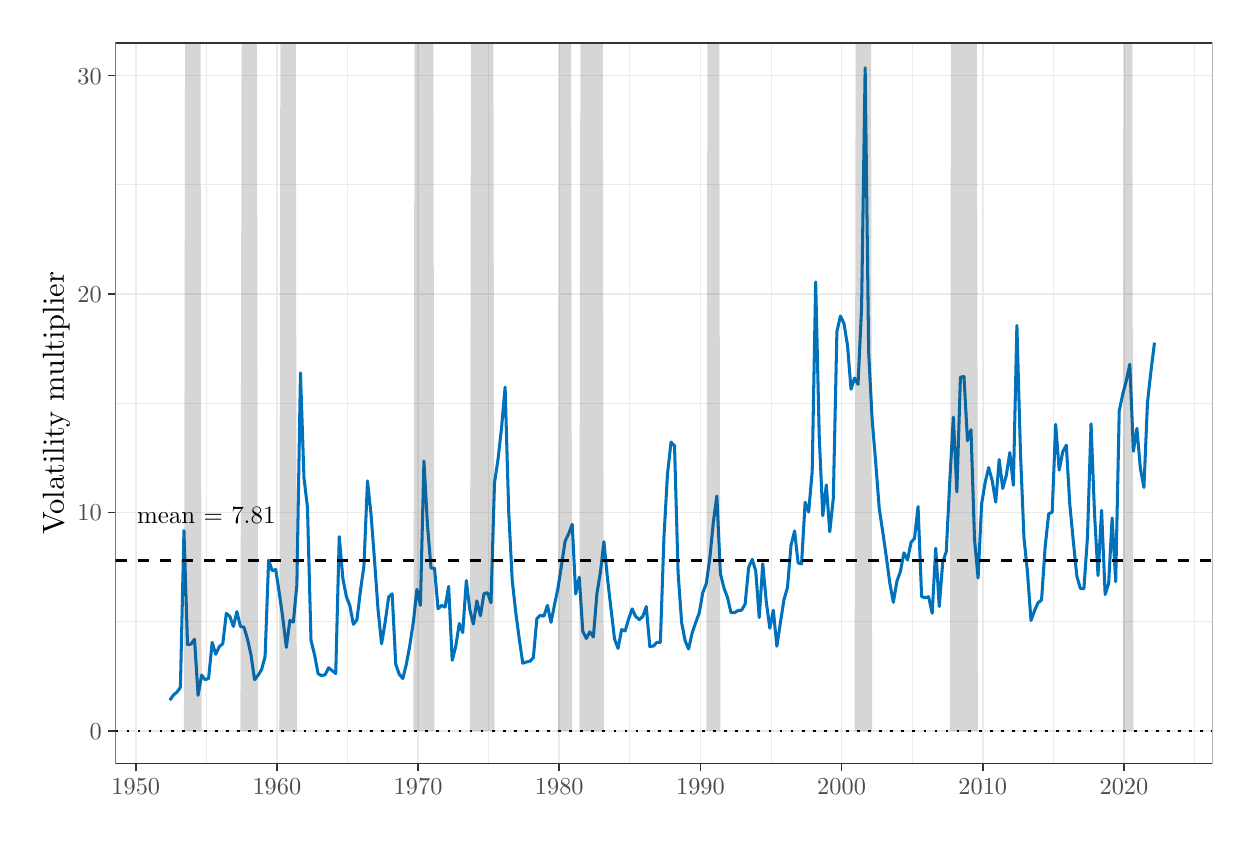
\begin{tikzpicture}[x=1pt,y=1pt]
\definecolor{fillColor}{RGB}{255,255,255}
\path[use as bounding box,fill=fillColor,fill opacity=0.00] (0,0) rectangle (433.62,289.08);
\begin{scope}
\path[clip] (  0.00,  0.00) rectangle (433.62,289.08);
\definecolor{drawColor}{RGB}{255,255,255}
\definecolor{fillColor}{RGB}{255,255,255}

\path[draw=drawColor,line width= 0.6pt,line join=round,line cap=round,fill=fillColor] (  0.00,  0.00) rectangle (433.62,289.08);
\end{scope}
\begin{scope}
\path[clip] ( 31.71, 23.11) rectangle (428.12,283.58);
\definecolor{fillColor}{RGB}{255,255,255}

\path[fill=fillColor] ( 31.71, 23.11) rectangle (428.12,283.58);
\definecolor{drawColor}{gray}{0.92}

\path[draw=drawColor,line width= 0.3pt,line join=round] ( 31.71, 74.41) --
	(428.12, 74.41);

\path[draw=drawColor,line width= 0.3pt,line join=round] ( 31.71,153.34) --
	(428.12,153.34);

\path[draw=drawColor,line width= 0.3pt,line join=round] ( 31.71,232.28) --
	(428.12,232.28);

\path[draw=drawColor,line width= 0.3pt,line join=round] ( 64.56, 23.11) --
	( 64.56,283.58);

\path[draw=drawColor,line width= 0.3pt,line join=round] (115.57, 23.11) --
	(115.57,283.58);

\path[draw=drawColor,line width= 0.3pt,line join=round] (166.59, 23.11) --
	(166.59,283.58);

\path[draw=drawColor,line width= 0.3pt,line join=round] (217.60, 23.11) --
	(217.60,283.58);

\path[draw=drawColor,line width= 0.3pt,line join=round] (268.61, 23.11) --
	(268.61,283.58);

\path[draw=drawColor,line width= 0.3pt,line join=round] (319.62, 23.11) --
	(319.62,283.58);

\path[draw=drawColor,line width= 0.3pt,line join=round] (370.64, 23.11) --
	(370.64,283.58);

\path[draw=drawColor,line width= 0.3pt,line join=round] (421.64, 23.11) --
	(421.64,283.58);

\path[draw=drawColor,line width= 0.6pt,line join=round] ( 31.71, 34.95) --
	(428.12, 34.95);

\path[draw=drawColor,line width= 0.6pt,line join=round] ( 31.71,113.88) --
	(428.12,113.88);

\path[draw=drawColor,line width= 0.6pt,line join=round] ( 31.71,192.81) --
	(428.12,192.81);

\path[draw=drawColor,line width= 0.6pt,line join=round] ( 31.71,271.74) --
	(428.12,271.74);

\path[draw=drawColor,line width= 0.6pt,line join=round] ( 39.06, 23.11) --
	( 39.06,283.58);

\path[draw=drawColor,line width= 0.6pt,line join=round] ( 90.06, 23.11) --
	( 90.06,283.58);

\path[draw=drawColor,line width= 0.6pt,line join=round] (141.08, 23.11) --
	(141.08,283.58);

\path[draw=drawColor,line width= 0.6pt,line join=round] (192.09, 23.11) --
	(192.09,283.58);

\path[draw=drawColor,line width= 0.6pt,line join=round] (243.11, 23.11) --
	(243.11,283.58);

\path[draw=drawColor,line width= 0.6pt,line join=round] (294.11, 23.11) --
	(294.11,283.58);

\path[draw=drawColor,line width= 0.6pt,line join=round] (345.13, 23.11) --
	(345.13,283.58);

\path[draw=drawColor,line width= 0.6pt,line join=round] (396.14, 23.11) --
	(396.14,283.58);
\definecolor{drawColor}{RGB}{0,114,189}

\path[draw=drawColor,line width= 1.1pt,line join=round] ( 51.38, 46.04) --
	( 52.66, 47.92) --
	( 53.93, 48.94) --
	( 55.19, 50.73) --
	( 56.47,107.36) --
	( 57.76, 66.17) --
	( 59.03, 66.34) --
	( 60.29, 68.09) --
	( 61.57, 47.82) --
	( 62.86, 55.13) --
	( 64.13, 53.47) --
	( 65.38, 53.96) --
	( 66.67, 66.96) --
	( 67.95, 62.65) --
	( 69.22, 65.38) --
	( 70.50, 66.45) --
	( 71.78, 77.44) --
	( 73.07, 76.31) --
	( 74.34, 72.68) --
	( 75.59, 78.09) --
	( 76.88, 72.69) --
	( 78.16, 72.45) --
	( 79.43, 68.14) --
	( 80.69, 62.51) --
	( 81.98, 53.49) --
	( 83.26, 55.04) --
	( 84.53, 57.15) --
	( 85.79, 61.88) --
	( 87.07, 96.65) --
	( 88.36, 92.86) --
	( 89.63, 93.25) --
	( 90.90, 84.90) --
	( 92.19, 75.80) --
	( 93.47, 65.15) --
	( 94.74, 74.90) --
	( 96.00, 74.28) --
	( 97.28, 87.82) --
	( 98.57,164.32) --
	( 99.84,126.39) --
	(101.10,115.80) --
	(102.38, 67.66) --
	(103.67, 62.44) --
	(104.94, 55.65) --
	(106.19, 54.93) --
	(107.48, 55.25) --
	(108.76, 57.79) --
	(110.03, 56.74) --
	(111.31, 55.69) --
	(112.59,105.19) --
	(113.88, 90.17) --
	(115.15, 83.51) --
	(116.40, 80.30) --
	(117.69, 73.48) --
	(118.97, 75.10) --
	(120.24, 85.61) --
	(121.50, 94.53) --
	(122.79,125.28) --
	(124.07,113.29) --
	(125.34, 96.52) --
	(126.60, 78.82) --
	(127.88, 66.42) --
	(129.17, 74.21) --
	(130.44, 83.33) --
	(131.71, 84.53) --
	(133.00, 59.04) --
	(134.28, 55.40) --
	(135.55, 53.88) --
	(136.81, 59.00) --
	(138.09, 65.88) --
	(139.38, 74.47) --
	(140.65, 86.13) --
	(141.91, 80.35) --
	(143.19,132.47) --
	(144.48,109.11) --
	(145.75, 93.79) --
	(147.00, 93.81) --
	(148.29, 79.11) --
	(149.57, 80.33) --
	(150.84, 79.69) --
	(152.12, 87.19) --
	(153.40, 60.48) --
	(154.69, 65.54) --
	(155.96, 73.79) --
	(157.21, 70.50) --
	(158.50, 89.30) --
	(159.78, 78.62) --
	(161.05, 73.57) --
	(162.31, 81.95) --
	(163.60, 76.57) --
	(164.88, 84.54) --
	(166.15, 84.92) --
	(167.41, 81.25) --
	(168.69,124.67) --
	(169.98,133.24) --
	(171.25,144.72) --
	(172.52,159.20) --
	(173.81,114.41) --
	(175.09, 89.36) --
	(176.36, 77.86) --
	(177.62, 68.31) --
	(178.90, 59.44) --
	(180.19, 59.86) --
	(181.46, 60.11) --
	(182.72, 61.41) --
	(184.00, 75.59) --
	(185.29, 76.77) --
	(186.56, 76.43) --
	(187.81, 80.34) --
	(189.10, 74.19) --
	(190.38, 80.62) --
	(191.65, 86.70) --
	(192.93, 95.02) --
	(194.21,103.55) --
	(195.50,106.24) --
	(196.77,109.62) --
	(198.02, 84.44) --
	(199.31, 90.53) --
	(200.59, 70.97) --
	(201.86, 68.37) --
	(203.12, 70.77) --
	(204.41, 68.90) --
	(205.69, 84.51) --
	(206.96, 92.28) --
	(208.22,103.34) --
	(209.50, 90.26) --
	(210.79, 79.02) --
	(212.06, 68.19) --
	(213.33, 64.78) --
	(214.62, 71.59) --
	(215.90, 71.11) --
	(217.17, 75.45) --
	(218.43, 79.06) --
	(219.71, 76.33) --
	(221.00, 75.14) --
	(222.27, 76.35) --
	(223.53, 79.89) --
	(224.81, 65.43) --
	(226.10, 65.65) --
	(227.37, 66.94) --
	(228.62, 66.92) --
	(229.91,104.88) --
	(231.19,127.79) --
	(232.47,139.32) --
	(233.74,137.96) --
	(235.02, 92.13) --
	(236.31, 74.07) --
	(237.58, 67.51) --
	(238.83, 64.58) --
	(240.12, 70.42) --
	(241.40, 74.14) --
	(242.67, 77.61) --
	(243.93, 84.85) --
	(245.22, 88.23) --
	(246.50, 97.43) --
	(247.77,110.46) --
	(249.03,119.86) --
	(250.31, 91.89) --
	(251.60, 86.58) --
	(252.87, 83.20) --
	(254.14, 77.70) --
	(255.43, 77.71) --
	(256.71, 78.46) --
	(257.98, 78.60) --
	(259.24, 80.78) --
	(260.52, 94.01) --
	(261.81, 96.94) --
	(263.08, 92.79) --
	(264.34, 75.94) --
	(265.62, 95.34) --
	(266.91, 81.41) --
	(268.18, 72.06) --
	(269.43, 78.57) --
	(270.72, 65.55) --
	(272.00, 74.10) --
	(273.28, 82.34) --
	(274.55, 86.82) --
	(275.83,102.05) --
	(277.12,107.22) --
	(278.39, 95.68) --
	(279.64, 95.33) --
	(280.93,117.59) --
	(282.21,114.06) --
	(283.48,128.77) --
	(284.74,197.19) --
	(286.03,141.29) --
	(287.31,112.71) --
	(288.58,123.87) --
	(289.84,106.92) --
	(291.12,119.08) --
	(292.41,179.23) --
	(293.68,184.88) --
	(294.95,182.22) --
	(296.24,174.31) --
	(297.52,158.42) --
	(298.79,162.48) --
	(300.05,160.19) --
	(301.33,187.92) --
	(302.62,274.60) --
	(303.89,171.71) --
	(305.15,147.57) --
	(306.43,131.95) --
	(307.72,115.27) --
	(308.99,106.81) --
	(310.24, 98.00) --
	(311.53, 88.40) --
	(312.81, 81.43) --
	(314.09, 89.07) --
	(315.36, 92.56) --
	(316.64, 99.33) --
	(317.93, 96.72) --
	(319.20,103.10) --
	(320.45,104.53) --
	(321.74,116.02) --
	(323.02, 83.51) --
	(324.29, 83.06) --
	(325.55, 83.43) --
	(326.84, 77.46) --
	(328.12,100.99) --
	(329.39, 79.90) --
	(330.65, 95.92) --
	(331.93, 99.75) --
	(333.22,125.71) --
	(334.49,148.38) --
	(335.76,121.34) --
	(337.05,162.78) --
	(338.33,163.01) --
	(339.60,139.83) --
	(340.86,143.81) --
	(342.14,104.14) --
	(343.43, 90.21) --
	(344.70,116.95) --
	(345.96,124.65) --
	(347.24,130.15) --
	(348.53,125.38) --
	(349.80,117.64) --
	(351.05,133.01) --
	(352.34,122.57) --
	(353.62,127.25) --
	(354.90,135.57) --
	(356.17,123.71) --
	(357.45,181.47) --
	(358.74,135.49) --
	(360.01,104.75) --
	(361.26, 92.42) --
	(362.55, 74.86) --
	(363.83, 78.44) --
	(365.10, 81.29) --
	(366.36, 82.26) --
	(367.65,101.35) --
	(368.93,113.41) --
	(370.20,113.98) --
	(371.46,145.74) --
	(372.74,129.18) --
	(374.03,135.87) --
	(375.30,138.21) --
	(376.57,116.84) --
	(377.86,103.29) --
	(379.14, 90.72) --
	(380.41, 86.41) --
	(381.67, 86.35) --
	(382.95,104.94) --
	(384.24,145.94) --
	(385.51,113.26) --
	(386.77, 91.11) --
	(388.05,114.68) --
	(389.34, 84.25) --
	(390.61, 88.31) --
	(391.86,111.92) --
	(393.15, 88.88) --
	(394.43,150.61) --
	(395.71,156.70) --
	(396.98,161.47) --
	(398.26,167.46) --
	(399.55,136.03) --
	(400.82,144.31) --
	(402.07,129.83) --
	(403.36,122.94) --
	(404.64,153.67) --
	(405.91,165.12) --
	(407.17,175.26);
\definecolor{fillColor}{RGB}{51,51,51}

\path[fill=fillColor,fill opacity=0.20] ( 50.09, 34.95) --
	( 50.45, 34.95) --
	( 51.02, 34.95) --
	( 51.38, 34.95) --
	( 51.73, 34.95) --
	( 52.30, 34.95) --
	( 52.66, 34.95) --
	( 53.02, 34.95) --
	( 53.57, 34.95) --
	( 53.93, 34.95) --
	( 54.29, 34.95) --
	( 54.83, 34.95) --
	( 55.19, 34.95) --
	( 55.55, 34.95) --
	( 56.11, 34.95) --
	( 56.47, 34.95) --
	( 56.83,255.88) --
	( 57.40,603.33) --
	( 57.76,824.25) --
	( 58.12,824.25) --
	( 58.67,824.25) --
	( 59.03,824.25) --
	( 59.39,824.25) --
	( 59.93,824.25) --
	( 60.29,824.25) --
	( 60.65,824.25) --
	( 61.21,824.25) --
	( 61.57,824.25) --
	( 61.93,603.33) --
	( 62.50,255.88) --
	( 62.86, 34.95) --
	( 63.22, 34.95) --
	( 63.77, 34.95) --
	( 64.13, 34.95) --
	( 64.49, 34.95) --
	( 65.02, 34.95) --
	( 65.38, 34.95) --
	( 65.74, 34.95) --
	( 66.31, 34.95) --
	( 66.67, 34.95) --
	( 67.03, 34.95) --
	( 67.59, 34.95) --
	( 67.95, 34.95) --
	( 68.31, 34.95) --
	( 68.86, 34.95) --
	( 69.22, 34.95) --
	( 69.58, 34.95) --
	( 70.14, 34.95) --
	( 70.50, 34.95) --
	( 70.86, 34.95) --
	( 71.42, 34.95) --
	( 71.78, 34.95) --
	( 72.14, 34.95) --
	( 72.71, 34.95) --
	( 73.07, 34.95) --
	( 73.42, 34.95) --
	( 73.98, 34.95) --
	( 74.34, 34.95) --
	( 74.70, 34.95) --
	( 75.23, 34.95) --
	( 75.59, 34.95) --
	( 75.95, 34.95) --
	( 76.52, 34.95) --
	( 76.88, 34.95) --
	( 77.24,255.88) --
	( 77.80,603.33) --
	( 78.16,824.25) --
	( 78.52,824.25) --
	( 79.07,824.25) --
	( 79.43,824.25) --
	( 79.79,824.25) --
	( 80.33,824.25) --
	( 80.69,824.25) --
	( 81.05,824.25) --
	( 81.62,824.25) --
	( 81.98,824.25) --
	( 82.34,603.33) --
	( 82.90,255.88) --
	( 83.26, 34.95) --
	( 83.62, 34.95) --
	( 84.17, 34.95) --
	( 84.53, 34.95) --
	( 84.89, 34.95) --
	( 85.43, 34.95) --
	( 85.79, 34.95) --
	( 86.15, 34.95) --
	( 86.71, 34.95) --
	( 87.07, 34.95) --
	( 87.43, 34.95) --
	( 88.00, 34.95) --
	( 88.36, 34.95) --
	( 88.72, 34.95) --
	( 89.27, 34.95) --
	( 89.63, 34.95) --
	( 89.99, 34.95) --
	( 90.54, 34.95) --
	( 90.90, 34.95) --
	( 91.26,255.88) --
	( 91.83,603.33) --
	( 92.19,824.25) --
	( 92.55,824.25) --
	( 93.11,824.25) --
	( 93.47,824.25) --
	( 93.83,824.25) --
	( 94.38,824.25) --
	( 94.74,824.25) --
	( 95.10,824.25) --
	( 95.64,824.25) --
	( 96.00,824.25) --
	( 96.36,603.33) --
	( 96.92,255.88) --
	( 97.28, 34.95) --
	( 97.64, 34.95) --
	( 98.21, 34.95) --
	( 98.57, 34.95) --
	( 98.93, 34.95) --
	( 99.48, 34.95) --
	( 99.84, 34.95) --
	(100.20, 34.95) --
	(100.74, 34.95) --
	(101.10, 34.95) --
	(101.46, 34.95) --
	(102.02, 34.95) --
	(102.38, 34.95) --
	(102.74, 34.95) --
	(103.31, 34.95) --
	(103.67, 34.95) --
	(104.03, 34.95) --
	(104.58, 34.95) --
	(104.94, 34.95) --
	(105.30, 34.95) --
	(105.83, 34.95) --
	(106.19, 34.95) --
	(106.55, 34.95) --
	(107.12, 34.95) --
	(107.48, 34.95) --
	(107.84, 34.95) --
	(108.40, 34.95) --
	(108.76, 34.95) --
	(109.12, 34.95) --
	(109.67, 34.95) --
	(110.03, 34.95) --
	(110.39, 34.95) --
	(110.95, 34.95) --
	(111.31, 34.95) --
	(111.67, 34.95) --
	(112.23, 34.95) --
	(112.59, 34.95) --
	(112.95, 34.95) --
	(113.52, 34.95) --
	(113.88, 34.95) --
	(114.24, 34.95) --
	(114.79, 34.95) --
	(115.15, 34.95) --
	(115.51, 34.95) --
	(116.04, 34.95) --
	(116.40, 34.95) --
	(116.76, 34.95) --
	(117.33, 34.95) --
	(117.69, 34.95) --
	(118.05, 34.95) --
	(118.61, 34.95) --
	(118.97, 34.95) --
	(119.33, 34.95) --
	(119.88, 34.95) --
	(120.24, 34.95) --
	(120.60, 34.95) --
	(121.14, 34.95) --
	(121.50, 34.95) --
	(121.86, 34.95) --
	(122.43, 34.95) --
	(122.79, 34.95) --
	(123.15, 34.95) --
	(123.71, 34.95) --
	(124.07, 34.95) --
	(124.43, 34.95) --
	(124.98, 34.95) --
	(125.34, 34.95) --
	(125.70, 34.95) --
	(126.24, 34.95) --
	(126.60, 34.95) --
	(126.96, 34.95) --
	(127.52, 34.95) --
	(127.88, 34.95) --
	(128.24, 34.95) --
	(128.81, 34.95) --
	(129.17, 34.95) --
	(129.53, 34.95) --
	(130.08, 34.95) --
	(130.44, 34.95) --
	(130.80, 34.95) --
	(131.35, 34.95) --
	(131.71, 34.95) --
	(132.07, 34.95) --
	(132.64, 34.95) --
	(133.00, 34.95) --
	(133.36, 34.95) --
	(133.92, 34.95) --
	(134.28, 34.95) --
	(134.64, 34.95) --
	(135.19, 34.95) --
	(135.55, 34.95) --
	(135.91, 34.95) --
	(136.45, 34.95) --
	(136.81, 34.95) --
	(137.17, 34.95) --
	(137.73, 34.95) --
	(138.09, 34.95) --
	(138.45, 34.95) --
	(139.02, 34.95) --
	(139.38, 34.95) --
	(139.74,258.30) --
	(140.29,600.90) --
	(140.65,824.25) --
	(141.01,824.25) --
	(141.55,824.25) --
	(141.91,824.25) --
	(142.27,824.25) --
	(142.83,824.25) --
	(143.19,824.25) --
	(143.55,824.25) --
	(144.12,824.25) --
	(144.48,824.25) --
	(144.84,824.25) --
	(145.39,824.25) --
	(145.75,824.25) --
	(146.11,598.42) --
	(146.64,260.79) --
	(147.00, 34.95) --
	(147.36, 34.95) --
	(147.93, 34.95) --
	(148.29, 34.95) --
	(148.65, 34.95) --
	(149.21, 34.95) --
	(149.57, 34.95) --
	(149.93, 34.95) --
	(150.49, 34.95) --
	(150.84, 34.95) --
	(151.20, 34.95) --
	(151.76, 34.95) --
	(152.12, 34.95) --
	(152.48, 34.95) --
	(153.04, 34.95) --
	(153.40, 34.95) --
	(153.76, 34.95) --
	(154.33, 34.95) --
	(154.69, 34.95) --
	(155.05, 34.95) --
	(155.60, 34.95) --
	(155.96, 34.95) --
	(156.32, 34.95) --
	(156.85, 34.95) --
	(157.21, 34.95) --
	(157.57, 34.95) --
	(158.14, 34.95) --
	(158.50, 34.95) --
	(158.86, 34.95) --
	(159.42, 34.95) --
	(159.78, 34.95) --
	(160.14,258.30) --
	(160.69,600.90) --
	(161.05,824.25) --
	(161.41,824.25) --
	(161.95,824.25) --
	(162.31,824.25) --
	(162.67,824.25) --
	(163.24,824.25) --
	(163.60,824.25) --
	(163.96,824.25) --
	(164.52,824.25) --
	(164.88,824.25) --
	(165.24,824.25) --
	(165.79,824.25) --
	(166.15,824.25) --
	(166.51,824.25) --
	(167.05,824.25) --
	(167.41,824.25) --
	(167.77,603.33) --
	(168.33,255.88) --
	(168.69, 34.95) --
	(169.05, 34.95) --
	(169.62, 34.95) --
	(169.98, 34.95) --
	(170.34, 34.95) --
	(170.89, 34.95) --
	(171.25, 34.95) --
	(171.61, 34.95) --
	(172.16, 34.95) --
	(172.52, 34.95) --
	(172.88, 34.95) --
	(173.45, 34.95) --
	(173.81, 34.95) --
	(174.17, 34.95) --
	(174.73, 34.95) --
	(175.09, 34.95) --
	(175.45, 34.95) --
	(176.00, 34.95) --
	(176.36, 34.95) --
	(176.72, 34.95) --
	(177.26, 34.95) --
	(177.62, 34.95) --
	(177.98, 34.95) --
	(178.54, 34.95) --
	(178.90, 34.95) --
	(179.26, 34.95) --
	(179.83, 34.95) --
	(180.19, 34.95) --
	(180.55, 34.95) --
	(181.10, 34.95) --
	(181.46, 34.95) --
	(181.82, 34.95) --
	(182.36, 34.95) --
	(182.72, 34.95) --
	(183.08, 34.95) --
	(183.64, 34.95) --
	(184.00, 34.95) --
	(184.36, 34.95) --
	(184.93, 34.95) --
	(185.29, 34.95) --
	(185.65, 34.95) --
	(186.20, 34.95) --
	(186.56, 34.95) --
	(186.92, 34.95) --
	(187.45, 34.95) --
	(187.81, 34.95) --
	(188.17, 34.95) --
	(188.74, 34.95) --
	(189.10, 34.95) --
	(189.46, 34.95) --
	(190.02, 34.95) --
	(190.38, 34.95) --
	(190.74, 34.95) --
	(191.30, 34.95) --
	(191.65, 34.95) --
	(192.01,258.30) --
	(192.57,600.90) --
	(192.93,824.25) --
	(193.29,824.25) --
	(193.85,824.25) --
	(194.21,824.25) --
	(194.57,824.25) --
	(195.14,824.25) --
	(195.50,824.25) --
	(195.86,600.90) --
	(196.41,258.30) --
	(196.77, 34.95) --
	(197.13, 34.95) --
	(197.66, 34.95) --
	(198.02, 34.95) --
	(198.38, 34.95) --
	(198.95, 34.95) --
	(199.31, 34.95) --
	(199.67,255.88) --
	(200.23,603.33) --
	(200.59,824.25) --
	(200.95,824.25) --
	(201.50,824.25) --
	(201.86,824.25) --
	(202.22,824.25) --
	(202.76,824.25) --
	(203.12,824.25) --
	(203.48,824.25) --
	(204.05,824.25) --
	(204.41,824.25) --
	(204.77,824.25) --
	(205.33,824.25) --
	(205.69,824.25) --
	(206.05,824.25) --
	(206.60,824.25) --
	(206.96,824.25) --
	(207.32,598.42) --
	(207.86,260.79) --
	(208.22, 34.95) --
	(208.58, 34.95) --
	(209.14, 34.95) --
	(209.50, 34.95) --
	(209.86, 34.95) --
	(210.43, 34.95) --
	(210.79, 34.95) --
	(211.15, 34.95) --
	(211.70, 34.95) --
	(212.06, 34.95) --
	(212.42, 34.95) --
	(212.97, 34.95) --
	(213.33, 34.95) --
	(213.69, 34.95) --
	(214.26, 34.95) --
	(214.62, 34.95) --
	(214.98, 34.95) --
	(215.54, 34.95) --
	(215.90, 34.95) --
	(216.26, 34.95) --
	(216.81, 34.95) --
	(217.17, 34.95) --
	(217.53, 34.95) --
	(218.07, 34.95) --
	(218.43, 34.95) --
	(218.79, 34.95) --
	(219.35, 34.95) --
	(219.71, 34.95) --
	(220.07, 34.95) --
	(220.64, 34.95) --
	(221.00, 34.95) --
	(221.36, 34.95) --
	(221.91, 34.95) --
	(222.27, 34.95) --
	(222.63, 34.95) --
	(223.17, 34.95) --
	(223.53, 34.95) --
	(223.89, 34.95) --
	(224.45, 34.95) --
	(224.81, 34.95) --
	(225.17, 34.95) --
	(225.74, 34.95) --
	(226.10, 34.95) --
	(226.46, 34.95) --
	(227.01, 34.95) --
	(227.37, 34.95) --
	(227.73, 34.95) --
	(228.26, 34.95) --
	(228.62, 34.95) --
	(228.98, 34.95) --
	(229.55, 34.95) --
	(229.91, 34.95) --
	(230.27, 34.95) --
	(230.83, 34.95) --
	(231.19, 34.95) --
	(231.55, 34.95) --
	(232.11, 34.95) --
	(232.47, 34.95) --
	(232.82, 34.95) --
	(233.38, 34.95) --
	(233.74, 34.95) --
	(234.10, 34.95) --
	(234.66, 34.95) --
	(235.02, 34.95) --
	(235.38, 34.95) --
	(235.95, 34.95) --
	(236.31, 34.95) --
	(236.67, 34.95) --
	(237.22, 34.95) --
	(237.58, 34.95) --
	(237.94, 34.95) --
	(238.47, 34.95) --
	(238.83, 34.95) --
	(239.19, 34.95) --
	(239.76, 34.95) --
	(240.12, 34.95) --
	(240.48, 34.95) --
	(241.04, 34.95) --
	(241.40, 34.95) --
	(241.76, 34.95) --
	(242.31, 34.95) --
	(242.67, 34.95) --
	(243.03, 34.95) --
	(243.57, 34.95) --
	(243.93, 34.95) --
	(244.29, 34.95) --
	(244.86, 34.95) --
	(245.22, 34.95) --
	(245.58,255.88) --
	(246.14,603.33) --
	(246.50,824.25) --
	(246.86,824.25) --
	(247.41,824.25) --
	(247.77,824.25) --
	(248.13,824.25) --
	(248.67,824.25) --
	(249.03,824.25) --
	(249.39,603.33) --
	(249.95,255.88) --
	(250.31, 34.95) --
	(250.67, 34.95) --
	(251.24, 34.95) --
	(251.60, 34.95) --
	(251.96, 34.95) --
	(252.51, 34.95) --
	(252.87, 34.95) --
	(253.23, 34.95) --
	(253.78, 34.95) --
	(254.14, 34.95) --
	(254.50, 34.95) --
	(255.07, 34.95) --
	(255.43, 34.95) --
	(255.79, 34.95) --
	(256.35, 34.95) --
	(256.71, 34.95) --
	(257.07, 34.95) --
	(257.62, 34.95) --
	(257.98, 34.95) --
	(258.34, 34.95) --
	(258.88, 34.95) --
	(259.24, 34.95) --
	(259.60, 34.95) --
	(260.16, 34.95) --
	(260.52, 34.95) --
	(260.88, 34.95) --
	(261.45, 34.95) --
	(261.81, 34.95) --
	(262.17, 34.95) --
	(262.72, 34.95) --
	(263.08, 34.95) --
	(263.44, 34.95) --
	(263.98, 34.95) --
	(264.34, 34.95) --
	(264.70, 34.95) --
	(265.26, 34.95) --
	(265.62, 34.95) --
	(265.98, 34.95) --
	(266.55, 34.95) --
	(266.91, 34.95) --
	(267.27, 34.95) --
	(267.82, 34.95) --
	(268.18, 34.95) --
	(268.54, 34.95) --
	(269.07, 34.95) --
	(269.43, 34.95) --
	(269.79, 34.95) --
	(270.36, 34.95) --
	(270.72, 34.95) --
	(271.08, 34.95) --
	(271.64, 34.95) --
	(272.00, 34.95) --
	(272.36, 34.95) --
	(272.92, 34.95) --
	(273.28, 34.95) --
	(273.63, 34.95) --
	(274.19, 34.95) --
	(274.55, 34.95) --
	(274.91, 34.95) --
	(275.47, 34.95) --
	(275.83, 34.95) --
	(276.19, 34.95) --
	(276.76, 34.95) --
	(277.12, 34.95) --
	(277.48, 34.95) --
	(278.03, 34.95) --
	(278.39, 34.95) --
	(278.75, 34.95) --
	(279.28, 34.95) --
	(279.64, 34.95) --
	(280.00, 34.95) --
	(280.57, 34.95) --
	(280.93, 34.95) --
	(281.29, 34.95) --
	(281.85, 34.95) --
	(282.21, 34.95) --
	(282.57, 34.95) --
	(283.12, 34.95) --
	(283.48, 34.95) --
	(283.84, 34.95) --
	(284.38, 34.95) --
	(284.74, 34.95) --
	(285.10, 34.95) --
	(285.67, 34.95) --
	(286.03, 34.95) --
	(286.39, 34.95) --
	(286.95, 34.95) --
	(287.31, 34.95) --
	(287.67, 34.95) --
	(288.22, 34.95) --
	(288.58, 34.95) --
	(288.94, 34.95) --
	(289.48, 34.95) --
	(289.84, 34.95) --
	(290.20, 34.95) --
	(290.76, 34.95) --
	(291.12, 34.95) --
	(291.48, 34.95) --
	(292.05, 34.95) --
	(292.41, 34.95) --
	(292.77, 34.95) --
	(293.32, 34.95) --
	(293.68, 34.95) --
	(294.04, 34.95) --
	(294.59, 34.95) --
	(294.95, 34.95) --
	(295.31, 34.95) --
	(295.88, 34.95) --
	(296.24, 34.95) --
	(296.60, 34.95) --
	(297.16, 34.95) --
	(297.52, 34.95) --
	(297.88, 34.95) --
	(298.43, 34.95) --
	(298.79, 34.95) --
	(299.15,260.79) --
	(299.69,598.42) --
	(300.05,824.25) --
	(300.41,824.25) --
	(300.97,824.25) --
	(301.33,824.25) --
	(301.69,824.25) --
	(302.26,824.25) --
	(302.62,824.25) --
	(302.98,824.25) --
	(303.53,824.25) --
	(303.89,824.25) --
	(304.25,598.42) --
	(304.79,260.79) --
	(305.15, 34.95) --
	(305.51, 34.95) --
	(306.07, 34.95) --
	(306.43, 34.95) --
	(306.79, 34.95) --
	(307.36, 34.95) --
	(307.72, 34.95) --
	(308.08, 34.95) --
	(308.63, 34.95) --
	(308.99, 34.95) --
	(309.35, 34.95) --
	(309.88, 34.95) --
	(310.24, 34.95) --
	(310.60, 34.95) --
	(311.17, 34.95) --
	(311.53, 34.95) --
	(311.89, 34.95) --
	(312.45, 34.95) --
	(312.81, 34.95) --
	(313.17, 34.95) --
	(313.73, 34.95) --
	(314.09, 34.95) --
	(314.44, 34.95) --
	(315.00, 34.95) --
	(315.36, 34.95) --
	(315.72, 34.95) --
	(316.28, 34.95) --
	(316.64, 34.95) --
	(317.00, 34.95) --
	(317.57, 34.95) --
	(317.93, 34.95) --
	(318.29, 34.95) --
	(318.84, 34.95) --
	(319.20, 34.95) --
	(319.56, 34.95) --
	(320.09, 34.95) --
	(320.45, 34.95) --
	(320.81, 34.95) --
	(321.38, 34.95) --
	(321.74, 34.95) --
	(322.10, 34.95) --
	(322.66, 34.95) --
	(323.02, 34.95) --
	(323.38, 34.95) --
	(323.94, 34.95) --
	(324.29, 34.95) --
	(324.65, 34.95) --
	(325.19, 34.95) --
	(325.55, 34.95) --
	(325.91, 34.95) --
	(326.48, 34.95) --
	(326.84, 34.95) --
	(327.20, 34.95) --
	(327.76, 34.95) --
	(328.12, 34.95) --
	(328.48, 34.95) --
	(329.03, 34.95) --
	(329.39, 34.95) --
	(329.75, 34.95) --
	(330.29, 34.95) --
	(330.65, 34.95) --
	(331.01, 34.95) --
	(331.57, 34.95) --
	(331.93, 34.95) --
	(332.29, 34.95) --
	(332.86, 34.95) --
	(333.22, 34.95) --
	(333.58,258.30) --
	(334.13,600.90) --
	(334.49,824.25) --
	(334.85,824.25) --
	(335.40,824.25) --
	(335.76,824.25) --
	(336.12,824.25) --
	(336.69,824.25) --
	(337.05,824.25) --
	(337.41,824.25) --
	(337.97,824.25) --
	(338.33,824.25) --
	(338.69,824.25) --
	(339.24,824.25) --
	(339.60,824.25) --
	(339.96,824.25) --
	(340.50,824.25) --
	(340.86,824.25) --
	(341.22,824.25) --
	(341.78,824.25) --
	(342.14,824.25) --
	(342.50,603.33) --
	(343.07,255.88) --
	(343.43, 34.95) --
	(343.79, 34.95) --
	(344.34, 34.95) --
	(344.70, 34.95) --
	(345.06, 34.95) --
	(345.60, 34.95) --
	(345.96, 34.95) --
	(346.32, 34.95) --
	(346.88, 34.95) --
	(347.24, 34.95) --
	(347.60, 34.95) --
	(348.17, 34.95) --
	(348.53, 34.95) --
	(348.89, 34.95) --
	(349.44, 34.95) --
	(349.80, 34.95) --
	(350.16, 34.95) --
	(350.69, 34.95) --
	(351.05, 34.95) --
	(351.41, 34.95) --
	(351.98, 34.95) --
	(352.34, 34.95) --
	(352.70, 34.95) --
	(353.26, 34.95) --
	(353.62, 34.95) --
	(353.98, 34.95) --
	(354.54, 34.95) --
	(354.90, 34.95) --
	(355.26, 34.95) --
	(355.81, 34.95) --
	(356.17, 34.95) --
	(356.53, 34.95) --
	(357.09, 34.95) --
	(357.45, 34.95) --
	(357.81, 34.95) --
	(358.38, 34.95) --
	(358.74, 34.95) --
	(359.10, 34.95) --
	(359.65, 34.95) --
	(360.01, 34.95) --
	(360.37, 34.95) --
	(360.90, 34.95) --
	(361.26, 34.95) --
	(361.62, 34.95) --
	(362.19, 34.95) --
	(362.55, 34.95) --
	(362.91, 34.95) --
	(363.47, 34.95) --
	(363.83, 34.95) --
	(364.19, 34.95) --
	(364.75, 34.95) --
	(365.10, 34.95) --
	(365.46, 34.95) --
	(366.00, 34.95) --
	(366.36, 34.95) --
	(366.72, 34.95) --
	(367.29, 34.95) --
	(367.65, 34.95) --
	(368.01, 34.95) --
	(368.57, 34.95) --
	(368.93, 34.95) --
	(369.29, 34.95) --
	(369.84, 34.95) --
	(370.20, 34.95) --
	(370.56, 34.95) --
	(371.10, 34.95) --
	(371.46, 34.95) --
	(371.82, 34.95) --
	(372.38, 34.95) --
	(372.74, 34.95) --
	(373.10, 34.95) --
	(373.67, 34.95) --
	(374.03, 34.95) --
	(374.39, 34.95) --
	(374.94, 34.95) --
	(375.30, 34.95) --
	(375.66, 34.95) --
	(376.21, 34.95) --
	(376.57, 34.95) --
	(376.93, 34.95) --
	(377.50, 34.95) --
	(377.86, 34.95) --
	(378.22, 34.95) --
	(378.78, 34.95) --
	(379.14, 34.95) --
	(379.50, 34.95) --
	(380.05, 34.95) --
	(380.41, 34.95) --
	(380.77, 34.95) --
	(381.31, 34.95) --
	(381.67, 34.95) --
	(382.03, 34.95) --
	(382.59, 34.95) --
	(382.95, 34.95) --
	(383.31, 34.95) --
	(383.88, 34.95) --
	(384.24, 34.95) --
	(384.60, 34.95) --
	(385.15, 34.95) --
	(385.51, 34.95) --
	(385.87, 34.95) --
	(386.41, 34.95) --
	(386.77, 34.95) --
	(387.13, 34.95) --
	(387.69, 34.95) --
	(388.05, 34.95) --
	(388.41, 34.95) --
	(388.98, 34.95) --
	(389.34, 34.95) --
	(389.70, 34.95) --
	(390.25, 34.95) --
	(390.61, 34.95) --
	(390.97, 34.95) --
	(391.51, 34.95) --
	(391.86, 34.95) --
	(392.22, 34.95) --
	(392.79, 34.95) --
	(393.15, 34.95) --
	(393.51, 34.95) --
	(394.07, 34.95) --
	(394.43, 34.95) --
	(394.79, 34.95) --
	(395.35, 34.95) --
	(395.71, 34.95) --
	(396.07,258.30) --
	(396.62,600.90) --
	(396.98,824.25) --
	(397.34,824.25) --
	(397.90,824.25) --
	(398.26,824.25) --
	(398.62,603.33) --
	(399.19,255.88) --
	(399.55, 34.95) --
	(399.91, 34.95) --
	(400.46, 34.95) --
	(400.82, 34.95) --
	(401.18, 34.95) --
	(401.71, 34.95) --
	(402.07, 34.95) --
	(402.43, 34.95) --
	(403.00, 34.95) --
	(403.36, 34.95) --
	(403.72, 34.95) --
	(404.28, 34.95) --
	(404.64, 34.95) --
	(405.00, 34.95) --
	(405.56, 34.95) --
	(405.91, 34.95) --
	(406.27, 34.95) --
	(406.81, 34.95) --
	(407.17, 34.95) --
	(407.53, 34.95) --
	(408.10, 34.95) --
	(408.46, 34.95) --
	(408.82, 34.95) --
	(409.38, 34.95) --
	(409.74, 34.95) --
	(410.10, 34.95) --
	(409.74, 34.95) --
	(409.38, 34.95) --
	(408.82, 34.95) --
	(408.46, 34.95) --
	(408.10, 34.95) --
	(407.53, 34.95) --
	(407.17, 34.95) --
	(406.81, 34.95) --
	(406.27, 34.95) --
	(405.91, 34.95) --
	(405.56, 34.95) --
	(405.00, 34.95) --
	(404.64, 34.95) --
	(404.28, 34.95) --
	(403.72, 34.95) --
	(403.36, 34.95) --
	(403.00, 34.95) --
	(402.43, 34.95) --
	(402.07, 34.95) --
	(401.71, 34.95) --
	(401.18, 34.95) --
	(400.82, 34.95) --
	(400.46, 34.95) --
	(399.91, 34.95) --
	(399.55, 34.95) --
	(399.19, 34.95) --
	(398.62, 34.95) --
	(398.26, 34.95) --
	(397.90, 34.95) --
	(397.34, 34.95) --
	(396.98, 34.95) --
	(396.62, 34.95) --
	(396.07, 34.95) --
	(395.71, 34.95) --
	(395.35, 34.95) --
	(394.79, 34.95) --
	(394.43, 34.95) --
	(394.07, 34.95) --
	(393.51, 34.95) --
	(393.15, 34.95) --
	(392.79, 34.95) --
	(392.22, 34.95) --
	(391.86, 34.95) --
	(391.51, 34.95) --
	(390.97, 34.95) --
	(390.61, 34.95) --
	(390.25, 34.95) --
	(389.70, 34.95) --
	(389.34, 34.95) --
	(388.98, 34.95) --
	(388.41, 34.95) --
	(388.05, 34.95) --
	(387.69, 34.95) --
	(387.13, 34.95) --
	(386.77, 34.95) --
	(386.41, 34.95) --
	(385.87, 34.95) --
	(385.51, 34.95) --
	(385.15, 34.95) --
	(384.60, 34.95) --
	(384.24, 34.95) --
	(383.88, 34.95) --
	(383.31, 34.95) --
	(382.95, 34.95) --
	(382.59, 34.95) --
	(382.03, 34.95) --
	(381.67, 34.95) --
	(381.31, 34.95) --
	(380.77, 34.95) --
	(380.41, 34.95) --
	(380.05, 34.95) --
	(379.50, 34.95) --
	(379.14, 34.95) --
	(378.78, 34.95) --
	(378.22, 34.95) --
	(377.86, 34.95) --
	(377.50, 34.95) --
	(376.93, 34.95) --
	(376.57, 34.95) --
	(376.21, 34.95) --
	(375.66, 34.95) --
	(375.30, 34.95) --
	(374.94, 34.95) --
	(374.39, 34.95) --
	(374.03, 34.95) --
	(373.67, 34.95) --
	(373.10, 34.95) --
	(372.74, 34.95) --
	(372.38, 34.95) --
	(371.82, 34.95) --
	(371.46, 34.95) --
	(371.10, 34.95) --
	(370.56, 34.95) --
	(370.20, 34.95) --
	(369.84, 34.95) --
	(369.29, 34.95) --
	(368.93, 34.95) --
	(368.57, 34.95) --
	(368.01, 34.95) --
	(367.65, 34.95) --
	(367.29, 34.95) --
	(366.72, 34.95) --
	(366.36, 34.95) --
	(366.00, 34.95) --
	(365.46, 34.95) --
	(365.10, 34.95) --
	(364.75, 34.95) --
	(364.19, 34.95) --
	(363.83, 34.95) --
	(363.47, 34.95) --
	(362.91, 34.95) --
	(362.55, 34.95) --
	(362.19, 34.95) --
	(361.62, 34.95) --
	(361.26, 34.95) --
	(360.90, 34.95) --
	(360.37, 34.95) --
	(360.01, 34.95) --
	(359.65, 34.95) --
	(359.10, 34.95) --
	(358.74, 34.95) --
	(358.38, 34.95) --
	(357.81, 34.95) --
	(357.45, 34.95) --
	(357.09, 34.95) --
	(356.53, 34.95) --
	(356.17, 34.95) --
	(355.81, 34.95) --
	(355.26, 34.95) --
	(354.90, 34.95) --
	(354.54, 34.95) --
	(353.98, 34.95) --
	(353.62, 34.95) --
	(353.26, 34.95) --
	(352.70, 34.95) --
	(352.34, 34.95) --
	(351.98, 34.95) --
	(351.41, 34.95) --
	(351.05, 34.95) --
	(350.69, 34.95) --
	(350.16, 34.95) --
	(349.80, 34.95) --
	(349.44, 34.95) --
	(348.89, 34.95) --
	(348.53, 34.95) --
	(348.17, 34.95) --
	(347.60, 34.95) --
	(347.24, 34.95) --
	(346.88, 34.95) --
	(346.32, 34.95) --
	(345.96, 34.95) --
	(345.60, 34.95) --
	(345.06, 34.95) --
	(344.70, 34.95) --
	(344.34, 34.95) --
	(343.79, 34.95) --
	(343.43, 34.95) --
	(343.07, 34.95) --
	(342.50, 34.95) --
	(342.14, 34.95) --
	(341.78, 34.95) --
	(341.22, 34.95) --
	(340.86, 34.95) --
	(340.50, 34.95) --
	(339.96, 34.95) --
	(339.60, 34.95) --
	(339.24, 34.95) --
	(338.69, 34.95) --
	(338.33, 34.95) --
	(337.97, 34.95) --
	(337.41, 34.95) --
	(337.05, 34.95) --
	(336.69, 34.95) --
	(336.12, 34.95) --
	(335.76, 34.95) --
	(335.40, 34.95) --
	(334.85, 34.95) --
	(334.49, 34.95) --
	(334.13, 34.95) --
	(333.58, 34.95) --
	(333.22, 34.95) --
	(332.86, 34.95) --
	(332.29, 34.95) --
	(331.93, 34.95) --
	(331.57, 34.95) --
	(331.01, 34.95) --
	(330.65, 34.95) --
	(330.29, 34.95) --
	(329.75, 34.95) --
	(329.39, 34.95) --
	(329.03, 34.95) --
	(328.48, 34.95) --
	(328.12, 34.95) --
	(327.76, 34.95) --
	(327.20, 34.95) --
	(326.84, 34.95) --
	(326.48, 34.95) --
	(325.91, 34.95) --
	(325.55, 34.95) --
	(325.19, 34.95) --
	(324.65, 34.95) --
	(324.29, 34.95) --
	(323.94, 34.95) --
	(323.38, 34.95) --
	(323.02, 34.95) --
	(322.66, 34.95) --
	(322.10, 34.95) --
	(321.74, 34.95) --
	(321.38, 34.95) --
	(320.81, 34.95) --
	(320.45, 34.95) --
	(320.09, 34.95) --
	(319.56, 34.95) --
	(319.20, 34.95) --
	(318.84, 34.95) --
	(318.29, 34.95) --
	(317.93, 34.95) --
	(317.57, 34.95) --
	(317.00, 34.95) --
	(316.64, 34.95) --
	(316.28, 34.95) --
	(315.72, 34.95) --
	(315.36, 34.95) --
	(315.00, 34.95) --
	(314.44, 34.95) --
	(314.09, 34.95) --
	(313.73, 34.95) --
	(313.17, 34.95) --
	(312.81, 34.95) --
	(312.45, 34.95) --
	(311.89, 34.95) --
	(311.53, 34.95) --
	(311.17, 34.95) --
	(310.60, 34.95) --
	(310.24, 34.95) --
	(309.88, 34.95) --
	(309.35, 34.95) --
	(308.99, 34.95) --
	(308.63, 34.95) --
	(308.08, 34.95) --
	(307.72, 34.95) --
	(307.36, 34.95) --
	(306.79, 34.95) --
	(306.43, 34.95) --
	(306.07, 34.95) --
	(305.51, 34.95) --
	(305.15, 34.95) --
	(304.79, 34.95) --
	(304.25, 34.95) --
	(303.89, 34.95) --
	(303.53, 34.95) --
	(302.98, 34.95) --
	(302.62, 34.95) --
	(302.26, 34.95) --
	(301.69, 34.95) --
	(301.33, 34.95) --
	(300.97, 34.95) --
	(300.41, 34.95) --
	(300.05, 34.95) --
	(299.69, 34.95) --
	(299.15, 34.95) --
	(298.79, 34.95) --
	(298.43, 34.95) --
	(297.88, 34.95) --
	(297.52, 34.95) --
	(297.16, 34.95) --
	(296.60, 34.95) --
	(296.24, 34.95) --
	(295.88, 34.95) --
	(295.31, 34.95) --
	(294.95, 34.95) --
	(294.59, 34.95) --
	(294.04, 34.95) --
	(293.68, 34.95) --
	(293.32, 34.95) --
	(292.77, 34.95) --
	(292.41, 34.95) --
	(292.05, 34.95) --
	(291.48, 34.95) --
	(291.12, 34.95) --
	(290.76, 34.95) --
	(290.20, 34.95) --
	(289.84, 34.95) --
	(289.48, 34.95) --
	(288.94, 34.95) --
	(288.58, 34.95) --
	(288.22, 34.95) --
	(287.67, 34.95) --
	(287.31, 34.95) --
	(286.95, 34.95) --
	(286.39, 34.95) --
	(286.03, 34.95) --
	(285.67, 34.95) --
	(285.10, 34.95) --
	(284.74, 34.95) --
	(284.38, 34.95) --
	(283.84, 34.95) --
	(283.48, 34.95) --
	(283.12, 34.95) --
	(282.57, 34.95) --
	(282.21, 34.95) --
	(281.85, 34.95) --
	(281.29, 34.95) --
	(280.93, 34.95) --
	(280.57, 34.95) --
	(280.00, 34.95) --
	(279.64, 34.95) --
	(279.28, 34.95) --
	(278.75, 34.95) --
	(278.39, 34.95) --
	(278.03, 34.95) --
	(277.48, 34.95) --
	(277.12, 34.95) --
	(276.76, 34.95) --
	(276.19, 34.95) --
	(275.83, 34.95) --
	(275.47, 34.95) --
	(274.91, 34.95) --
	(274.55, 34.95) --
	(274.19, 34.95) --
	(273.63, 34.95) --
	(273.28, 34.95) --
	(272.92, 34.95) --
	(272.36, 34.95) --
	(272.00, 34.95) --
	(271.64, 34.95) --
	(271.08, 34.95) --
	(270.72, 34.95) --
	(270.36, 34.95) --
	(269.79, 34.95) --
	(269.43, 34.95) --
	(269.07, 34.95) --
	(268.54, 34.95) --
	(268.18, 34.95) --
	(267.82, 34.95) --
	(267.27, 34.95) --
	(266.91, 34.95) --
	(266.55, 34.95) --
	(265.98, 34.95) --
	(265.62, 34.95) --
	(265.26, 34.95) --
	(264.70, 34.95) --
	(264.34, 34.95) --
	(263.98, 34.95) --
	(263.44, 34.95) --
	(263.08, 34.95) --
	(262.72, 34.95) --
	(262.17, 34.95) --
	(261.81, 34.95) --
	(261.45, 34.95) --
	(260.88, 34.95) --
	(260.52, 34.95) --
	(260.16, 34.95) --
	(259.60, 34.95) --
	(259.24, 34.95) --
	(258.88, 34.95) --
	(258.34, 34.95) --
	(257.98, 34.95) --
	(257.62, 34.95) --
	(257.07, 34.95) --
	(256.71, 34.95) --
	(256.35, 34.95) --
	(255.79, 34.95) --
	(255.43, 34.95) --
	(255.07, 34.95) --
	(254.50, 34.95) --
	(254.14, 34.95) --
	(253.78, 34.95) --
	(253.23, 34.95) --
	(252.87, 34.95) --
	(252.51, 34.95) --
	(251.96, 34.95) --
	(251.60, 34.95) --
	(251.24, 34.95) --
	(250.67, 34.95) --
	(250.31, 34.95) --
	(249.95, 34.95) --
	(249.39, 34.95) --
	(249.03, 34.95) --
	(248.67, 34.95) --
	(248.13, 34.95) --
	(247.77, 34.95) --
	(247.41, 34.95) --
	(246.86, 34.95) --
	(246.50, 34.95) --
	(246.14, 34.95) --
	(245.58, 34.95) --
	(245.22, 34.95) --
	(244.86, 34.95) --
	(244.29, 34.95) --
	(243.93, 34.95) --
	(243.57, 34.95) --
	(243.03, 34.95) --
	(242.67, 34.95) --
	(242.31, 34.95) --
	(241.76, 34.95) --
	(241.40, 34.95) --
	(241.04, 34.95) --
	(240.48, 34.95) --
	(240.12, 34.95) --
	(239.76, 34.95) --
	(239.19, 34.95) --
	(238.83, 34.95) --
	(238.47, 34.95) --
	(237.94, 34.95) --
	(237.58, 34.95) --
	(237.22, 34.95) --
	(236.67, 34.95) --
	(236.31, 34.95) --
	(235.95, 34.95) --
	(235.38, 34.95) --
	(235.02, 34.95) --
	(234.66, 34.95) --
	(234.10, 34.95) --
	(233.74, 34.95) --
	(233.38, 34.95) --
	(232.82, 34.95) --
	(232.47, 34.95) --
	(232.11, 34.95) --
	(231.55, 34.95) --
	(231.19, 34.95) --
	(230.83, 34.95) --
	(230.27, 34.95) --
	(229.91, 34.95) --
	(229.55, 34.95) --
	(228.98, 34.95) --
	(228.62, 34.95) --
	(228.26, 34.95) --
	(227.73, 34.95) --
	(227.37, 34.95) --
	(227.01, 34.95) --
	(226.46, 34.95) --
	(226.10, 34.95) --
	(225.74, 34.95) --
	(225.17, 34.95) --
	(224.81, 34.95) --
	(224.45, 34.95) --
	(223.89, 34.95) --
	(223.53, 34.95) --
	(223.17, 34.95) --
	(222.63, 34.95) --
	(222.27, 34.95) --
	(221.91, 34.95) --
	(221.36, 34.95) --
	(221.00, 34.95) --
	(220.64, 34.95) --
	(220.07, 34.95) --
	(219.71, 34.95) --
	(219.35, 34.95) --
	(218.79, 34.95) --
	(218.43, 34.95) --
	(218.07, 34.95) --
	(217.53, 34.95) --
	(217.17, 34.95) --
	(216.81, 34.95) --
	(216.26, 34.95) --
	(215.90, 34.95) --
	(215.54, 34.95) --
	(214.98, 34.95) --
	(214.62, 34.95) --
	(214.26, 34.95) --
	(213.69, 34.95) --
	(213.33, 34.95) --
	(212.97, 34.95) --
	(212.42, 34.95) --
	(212.06, 34.95) --
	(211.70, 34.95) --
	(211.15, 34.95) --
	(210.79, 34.95) --
	(210.43, 34.95) --
	(209.86, 34.95) --
	(209.50, 34.95) --
	(209.14, 34.95) --
	(208.58, 34.95) --
	(208.22, 34.95) --
	(207.86, 34.95) --
	(207.32, 34.95) --
	(206.96, 34.95) --
	(206.60, 34.95) --
	(206.05, 34.95) --
	(205.69, 34.95) --
	(205.33, 34.95) --
	(204.77, 34.95) --
	(204.41, 34.95) --
	(204.05, 34.95) --
	(203.48, 34.95) --
	(203.12, 34.95) --
	(202.76, 34.95) --
	(202.22, 34.95) --
	(201.86, 34.95) --
	(201.50, 34.95) --
	(200.95, 34.95) --
	(200.59, 34.95) --
	(200.23, 34.95) --
	(199.67, 34.95) --
	(199.31, 34.95) --
	(198.95, 34.95) --
	(198.38, 34.95) --
	(198.02, 34.95) --
	(197.66, 34.95) --
	(197.13, 34.95) --
	(196.77, 34.95) --
	(196.41, 34.95) --
	(195.86, 34.95) --
	(195.50, 34.95) --
	(195.14, 34.95) --
	(194.57, 34.95) --
	(194.21, 34.95) --
	(193.85, 34.95) --
	(193.29, 34.95) --
	(192.93, 34.95) --
	(192.57, 34.95) --
	(192.01, 34.95) --
	(191.65, 34.95) --
	(191.30, 34.95) --
	(190.74, 34.95) --
	(190.38, 34.95) --
	(190.02, 34.95) --
	(189.46, 34.95) --
	(189.10, 34.95) --
	(188.74, 34.95) --
	(188.17, 34.95) --
	(187.81, 34.95) --
	(187.45, 34.95) --
	(186.92, 34.95) --
	(186.56, 34.95) --
	(186.20, 34.95) --
	(185.65, 34.95) --
	(185.29, 34.95) --
	(184.93, 34.95) --
	(184.36, 34.95) --
	(184.00, 34.95) --
	(183.64, 34.95) --
	(183.08, 34.95) --
	(182.72, 34.95) --
	(182.36, 34.95) --
	(181.82, 34.95) --
	(181.46, 34.95) --
	(181.10, 34.95) --
	(180.55, 34.95) --
	(180.19, 34.95) --
	(179.83, 34.95) --
	(179.26, 34.95) --
	(178.90, 34.95) --
	(178.54, 34.95) --
	(177.98, 34.95) --
	(177.62, 34.95) --
	(177.26, 34.95) --
	(176.72, 34.95) --
	(176.36, 34.95) --
	(176.00, 34.95) --
	(175.45, 34.95) --
	(175.09, 34.95) --
	(174.73, 34.95) --
	(174.17, 34.95) --
	(173.81, 34.95) --
	(173.45, 34.95) --
	(172.88, 34.95) --
	(172.52, 34.95) --
	(172.16, 34.95) --
	(171.61, 34.95) --
	(171.25, 34.95) --
	(170.89, 34.95) --
	(170.34, 34.95) --
	(169.98, 34.95) --
	(169.62, 34.95) --
	(169.05, 34.95) --
	(168.69, 34.95) --
	(168.33, 34.95) --
	(167.77, 34.95) --
	(167.41, 34.95) --
	(167.05, 34.95) --
	(166.51, 34.95) --
	(166.15, 34.95) --
	(165.79, 34.95) --
	(165.24, 34.95) --
	(164.88, 34.95) --
	(164.52, 34.95) --
	(163.96, 34.95) --
	(163.60, 34.95) --
	(163.24, 34.95) --
	(162.67, 34.95) --
	(162.31, 34.95) --
	(161.95, 34.95) --
	(161.41, 34.95) --
	(161.05, 34.95) --
	(160.69, 34.95) --
	(160.14, 34.95) --
	(159.78, 34.95) --
	(159.42, 34.95) --
	(158.86, 34.95) --
	(158.50, 34.95) --
	(158.14, 34.95) --
	(157.57, 34.95) --
	(157.21, 34.95) --
	(156.85, 34.95) --
	(156.32, 34.95) --
	(155.96, 34.95) --
	(155.60, 34.95) --
	(155.05, 34.95) --
	(154.69, 34.95) --
	(154.33, 34.95) --
	(153.76, 34.95) --
	(153.40, 34.95) --
	(153.04, 34.95) --
	(152.48, 34.95) --
	(152.12, 34.95) --
	(151.76, 34.95) --
	(151.20, 34.95) --
	(150.84, 34.95) --
	(150.49, 34.95) --
	(149.93, 34.95) --
	(149.57, 34.95) --
	(149.21, 34.95) --
	(148.65, 34.95) --
	(148.29, 34.95) --
	(147.93, 34.95) --
	(147.36, 34.95) --
	(147.00, 34.95) --
	(146.64, 34.95) --
	(146.11, 34.95) --
	(145.75, 34.95) --
	(145.39, 34.95) --
	(144.84, 34.95) --
	(144.48, 34.95) --
	(144.12, 34.95) --
	(143.55, 34.95) --
	(143.19, 34.95) --
	(142.83, 34.95) --
	(142.27, 34.95) --
	(141.91, 34.95) --
	(141.55, 34.95) --
	(141.01, 34.95) --
	(140.65, 34.95) --
	(140.29, 34.95) --
	(139.74, 34.95) --
	(139.38, 34.95) --
	(139.02, 34.95) --
	(138.45, 34.95) --
	(138.09, 34.95) --
	(137.73, 34.95) --
	(137.17, 34.95) --
	(136.81, 34.95) --
	(136.45, 34.95) --
	(135.91, 34.95) --
	(135.55, 34.95) --
	(135.19, 34.95) --
	(134.64, 34.95) --
	(134.28, 34.95) --
	(133.92, 34.95) --
	(133.36, 34.95) --
	(133.00, 34.95) --
	(132.64, 34.95) --
	(132.07, 34.95) --
	(131.71, 34.95) --
	(131.35, 34.95) --
	(130.80, 34.95) --
	(130.44, 34.95) --
	(130.08, 34.95) --
	(129.53, 34.95) --
	(129.17, 34.95) --
	(128.81, 34.95) --
	(128.24, 34.95) --
	(127.88, 34.95) --
	(127.52, 34.95) --
	(126.96, 34.95) --
	(126.60, 34.95) --
	(126.24, 34.95) --
	(125.70, 34.95) --
	(125.34, 34.95) --
	(124.98, 34.95) --
	(124.43, 34.95) --
	(124.07, 34.95) --
	(123.71, 34.95) --
	(123.15, 34.95) --
	(122.79, 34.95) --
	(122.43, 34.95) --
	(121.86, 34.95) --
	(121.50, 34.95) --
	(121.14, 34.95) --
	(120.60, 34.95) --
	(120.24, 34.95) --
	(119.88, 34.95) --
	(119.33, 34.95) --
	(118.97, 34.95) --
	(118.61, 34.95) --
	(118.05, 34.95) --
	(117.69, 34.95) --
	(117.33, 34.95) --
	(116.76, 34.95) --
	(116.40, 34.95) --
	(116.04, 34.95) --
	(115.51, 34.95) --
	(115.15, 34.95) --
	(114.79, 34.95) --
	(114.24, 34.95) --
	(113.88, 34.95) --
	(113.52, 34.95) --
	(112.95, 34.95) --
	(112.59, 34.95) --
	(112.23, 34.95) --
	(111.67, 34.95) --
	(111.31, 34.95) --
	(110.95, 34.95) --
	(110.39, 34.95) --
	(110.03, 34.95) --
	(109.67, 34.95) --
	(109.12, 34.95) --
	(108.76, 34.95) --
	(108.40, 34.95) --
	(107.84, 34.95) --
	(107.48, 34.95) --
	(107.12, 34.95) --
	(106.55, 34.95) --
	(106.19, 34.95) --
	(105.83, 34.95) --
	(105.30, 34.95) --
	(104.94, 34.95) --
	(104.58, 34.95) --
	(104.03, 34.95) --
	(103.67, 34.95) --
	(103.31, 34.95) --
	(102.74, 34.95) --
	(102.38, 34.95) --
	(102.02, 34.95) --
	(101.46, 34.95) --
	(101.10, 34.95) --
	(100.74, 34.95) --
	(100.20, 34.95) --
	( 99.84, 34.95) --
	( 99.48, 34.95) --
	( 98.93, 34.95) --
	( 98.57, 34.95) --
	( 98.21, 34.95) --
	( 97.64, 34.95) --
	( 97.28, 34.95) --
	( 96.92, 34.95) --
	( 96.36, 34.95) --
	( 96.00, 34.95) --
	( 95.64, 34.95) --
	( 95.10, 34.95) --
	( 94.74, 34.95) --
	( 94.38, 34.95) --
	( 93.83, 34.95) --
	( 93.47, 34.95) --
	( 93.11, 34.95) --
	( 92.55, 34.95) --
	( 92.19, 34.95) --
	( 91.83, 34.95) --
	( 91.26, 34.95) --
	( 90.90, 34.95) --
	( 90.54, 34.95) --
	( 89.99, 34.95) --
	( 89.63, 34.95) --
	( 89.27, 34.95) --
	( 88.72, 34.95) --
	( 88.36, 34.95) --
	( 88.00, 34.95) --
	( 87.43, 34.95) --
	( 87.07, 34.95) --
	( 86.71, 34.95) --
	( 86.15, 34.95) --
	( 85.79, 34.95) --
	( 85.43, 34.95) --
	( 84.89, 34.95) --
	( 84.53, 34.95) --
	( 84.17, 34.95) --
	( 83.62, 34.95) --
	( 83.26, 34.95) --
	( 82.90, 34.95) --
	( 82.34, 34.95) --
	( 81.98, 34.95) --
	( 81.62, 34.95) --
	( 81.05, 34.95) --
	( 80.69, 34.95) --
	( 80.33, 34.95) --
	( 79.79, 34.95) --
	( 79.43, 34.95) --
	( 79.07, 34.95) --
	( 78.52, 34.95) --
	( 78.16, 34.95) --
	( 77.80, 34.95) --
	( 77.24, 34.95) --
	( 76.88, 34.95) --
	( 76.52, 34.95) --
	( 75.95, 34.95) --
	( 75.59, 34.95) --
	( 75.23, 34.95) --
	( 74.70, 34.95) --
	( 74.34, 34.95) --
	( 73.98, 34.95) --
	( 73.42, 34.95) --
	( 73.07, 34.95) --
	( 72.71, 34.95) --
	( 72.14, 34.95) --
	( 71.78, 34.95) --
	( 71.42, 34.95) --
	( 70.86, 34.95) --
	( 70.50, 34.95) --
	( 70.14, 34.95) --
	( 69.58, 34.95) --
	( 69.22, 34.95) --
	( 68.86, 34.95) --
	( 68.31, 34.95) --
	( 67.95, 34.95) --
	( 67.59, 34.95) --
	( 67.03, 34.95) --
	( 66.67, 34.95) --
	( 66.31, 34.95) --
	( 65.74, 34.95) --
	( 65.38, 34.95) --
	( 65.02, 34.95) --
	( 64.49, 34.95) --
	( 64.13, 34.95) --
	( 63.77, 34.95) --
	( 63.22, 34.95) --
	( 62.86, 34.95) --
	( 62.50, 34.95) --
	( 61.93, 34.95) --
	( 61.57, 34.95) --
	( 61.21, 34.95) --
	( 60.65, 34.95) --
	( 60.29, 34.95) --
	( 59.93, 34.95) --
	( 59.39, 34.95) --
	( 59.03, 34.95) --
	( 58.67, 34.95) --
	( 58.12, 34.95) --
	( 57.76, 34.95) --
	( 57.40, 34.95) --
	( 56.83, 34.95) --
	( 56.47, 34.95) --
	( 56.11, 34.95) --
	( 55.55, 34.95) --
	( 55.19, 34.95) --
	( 54.83, 34.95) --
	( 54.29, 34.95) --
	( 53.93, 34.95) --
	( 53.57, 34.95) --
	( 53.02, 34.95) --
	( 52.66, 34.95) --
	( 52.30, 34.95) --
	( 51.73, 34.95) --
	( 51.38, 34.95) --
	( 51.02, 34.95) --
	( 50.45, 34.95) --
	( 50.09, 34.95) --
	( 49.73, 34.95) --
	cycle;

\path[] ( 50.09, 34.95) --
	( 50.45, 34.95) --
	( 51.02, 34.95) --
	( 51.38, 34.95) --
	( 51.73, 34.95) --
	( 52.30, 34.95) --
	( 52.66, 34.95) --
	( 53.02, 34.95) --
	( 53.57, 34.95) --
	( 53.93, 34.95) --
	( 54.29, 34.95) --
	( 54.83, 34.95) --
	( 55.19, 34.95) --
	( 55.55, 34.95) --
	( 56.11, 34.95) --
	( 56.47, 34.95) --
	( 56.83,255.88) --
	( 57.40,603.33) --
	( 57.76,824.25) --
	( 58.12,824.25) --
	( 58.67,824.25) --
	( 59.03,824.25) --
	( 59.39,824.25) --
	( 59.93,824.25) --
	( 60.29,824.25) --
	( 60.65,824.25) --
	( 61.21,824.25) --
	( 61.57,824.25) --
	( 61.93,603.33) --
	( 62.50,255.88) --
	( 62.86, 34.95) --
	( 63.22, 34.95) --
	( 63.77, 34.95) --
	( 64.13, 34.95) --
	( 64.49, 34.95) --
	( 65.02, 34.95) --
	( 65.38, 34.95) --
	( 65.74, 34.95) --
	( 66.31, 34.95) --
	( 66.67, 34.95) --
	( 67.03, 34.95) --
	( 67.59, 34.95) --
	( 67.95, 34.95) --
	( 68.31, 34.95) --
	( 68.86, 34.95) --
	( 69.22, 34.95) --
	( 69.58, 34.95) --
	( 70.14, 34.95) --
	( 70.50, 34.95) --
	( 70.86, 34.95) --
	( 71.42, 34.95) --
	( 71.78, 34.95) --
	( 72.14, 34.95) --
	( 72.71, 34.95) --
	( 73.07, 34.95) --
	( 73.42, 34.95) --
	( 73.98, 34.95) --
	( 74.34, 34.95) --
	( 74.70, 34.95) --
	( 75.23, 34.95) --
	( 75.59, 34.95) --
	( 75.95, 34.95) --
	( 76.52, 34.95) --
	( 76.88, 34.95) --
	( 77.24,255.88) --
	( 77.80,603.33) --
	( 78.16,824.25) --
	( 78.52,824.25) --
	( 79.07,824.25) --
	( 79.43,824.25) --
	( 79.79,824.25) --
	( 80.33,824.25) --
	( 80.69,824.25) --
	( 81.05,824.25) --
	( 81.62,824.25) --
	( 81.98,824.25) --
	( 82.34,603.33) --
	( 82.90,255.88) --
	( 83.26, 34.95) --
	( 83.62, 34.95) --
	( 84.17, 34.95) --
	( 84.53, 34.95) --
	( 84.89, 34.95) --
	( 85.43, 34.95) --
	( 85.79, 34.95) --
	( 86.15, 34.95) --
	( 86.71, 34.95) --
	( 87.07, 34.95) --
	( 87.43, 34.95) --
	( 88.00, 34.95) --
	( 88.36, 34.95) --
	( 88.72, 34.95) --
	( 89.27, 34.95) --
	( 89.63, 34.95) --
	( 89.99, 34.95) --
	( 90.54, 34.95) --
	( 90.90, 34.95) --
	( 91.26,255.88) --
	( 91.83,603.33) --
	( 92.19,824.25) --
	( 92.55,824.25) --
	( 93.11,824.25) --
	( 93.47,824.25) --
	( 93.83,824.25) --
	( 94.38,824.25) --
	( 94.74,824.25) --
	( 95.10,824.25) --
	( 95.64,824.25) --
	( 96.00,824.25) --
	( 96.36,603.33) --
	( 96.92,255.88) --
	( 97.28, 34.95) --
	( 97.64, 34.95) --
	( 98.21, 34.95) --
	( 98.57, 34.95) --
	( 98.93, 34.95) --
	( 99.48, 34.95) --
	( 99.84, 34.95) --
	(100.20, 34.95) --
	(100.74, 34.95) --
	(101.10, 34.95) --
	(101.46, 34.95) --
	(102.02, 34.95) --
	(102.38, 34.95) --
	(102.74, 34.95) --
	(103.31, 34.95) --
	(103.67, 34.95) --
	(104.03, 34.95) --
	(104.58, 34.95) --
	(104.94, 34.95) --
	(105.30, 34.95) --
	(105.83, 34.95) --
	(106.19, 34.95) --
	(106.55, 34.95) --
	(107.12, 34.95) --
	(107.48, 34.95) --
	(107.84, 34.95) --
	(108.40, 34.95) --
	(108.76, 34.95) --
	(109.12, 34.95) --
	(109.67, 34.95) --
	(110.03, 34.95) --
	(110.39, 34.95) --
	(110.95, 34.95) --
	(111.31, 34.95) --
	(111.67, 34.95) --
	(112.23, 34.95) --
	(112.59, 34.95) --
	(112.95, 34.95) --
	(113.52, 34.95) --
	(113.88, 34.95) --
	(114.24, 34.95) --
	(114.79, 34.95) --
	(115.15, 34.95) --
	(115.51, 34.95) --
	(116.04, 34.95) --
	(116.40, 34.95) --
	(116.76, 34.95) --
	(117.33, 34.95) --
	(117.69, 34.95) --
	(118.05, 34.95) --
	(118.61, 34.95) --
	(118.97, 34.95) --
	(119.33, 34.95) --
	(119.88, 34.95) --
	(120.24, 34.95) --
	(120.60, 34.95) --
	(121.14, 34.95) --
	(121.50, 34.95) --
	(121.86, 34.95) --
	(122.43, 34.95) --
	(122.79, 34.95) --
	(123.15, 34.95) --
	(123.71, 34.95) --
	(124.07, 34.95) --
	(124.43, 34.95) --
	(124.98, 34.95) --
	(125.34, 34.95) --
	(125.70, 34.95) --
	(126.24, 34.95) --
	(126.60, 34.95) --
	(126.96, 34.95) --
	(127.52, 34.95) --
	(127.88, 34.95) --
	(128.24, 34.95) --
	(128.81, 34.95) --
	(129.17, 34.95) --
	(129.53, 34.95) --
	(130.08, 34.95) --
	(130.44, 34.95) --
	(130.80, 34.95) --
	(131.35, 34.95) --
	(131.71, 34.95) --
	(132.07, 34.95) --
	(132.64, 34.95) --
	(133.00, 34.95) --
	(133.36, 34.95) --
	(133.92, 34.95) --
	(134.28, 34.95) --
	(134.64, 34.95) --
	(135.19, 34.95) --
	(135.55, 34.95) --
	(135.91, 34.95) --
	(136.45, 34.95) --
	(136.81, 34.95) --
	(137.17, 34.95) --
	(137.73, 34.95) --
	(138.09, 34.95) --
	(138.45, 34.95) --
	(139.02, 34.95) --
	(139.38, 34.95) --
	(139.74,258.30) --
	(140.29,600.90) --
	(140.65,824.25) --
	(141.01,824.25) --
	(141.55,824.25) --
	(141.91,824.25) --
	(142.27,824.25) --
	(142.83,824.25) --
	(143.19,824.25) --
	(143.55,824.25) --
	(144.12,824.25) --
	(144.48,824.25) --
	(144.84,824.25) --
	(145.39,824.25) --
	(145.75,824.25) --
	(146.11,598.42) --
	(146.64,260.79) --
	(147.00, 34.95) --
	(147.36, 34.95) --
	(147.93, 34.95) --
	(148.29, 34.95) --
	(148.65, 34.95) --
	(149.21, 34.95) --
	(149.57, 34.95) --
	(149.93, 34.95) --
	(150.49, 34.95) --
	(150.84, 34.95) --
	(151.20, 34.95) --
	(151.76, 34.95) --
	(152.12, 34.95) --
	(152.48, 34.95) --
	(153.04, 34.95) --
	(153.40, 34.95) --
	(153.76, 34.95) --
	(154.33, 34.95) --
	(154.69, 34.95) --
	(155.05, 34.95) --
	(155.60, 34.95) --
	(155.96, 34.95) --
	(156.32, 34.95) --
	(156.85, 34.95) --
	(157.21, 34.95) --
	(157.57, 34.95) --
	(158.14, 34.95) --
	(158.50, 34.95) --
	(158.86, 34.95) --
	(159.42, 34.95) --
	(159.78, 34.95) --
	(160.14,258.30) --
	(160.69,600.90) --
	(161.05,824.25) --
	(161.41,824.25) --
	(161.95,824.25) --
	(162.31,824.25) --
	(162.67,824.25) --
	(163.24,824.25) --
	(163.60,824.25) --
	(163.96,824.25) --
	(164.52,824.25) --
	(164.88,824.25) --
	(165.24,824.25) --
	(165.79,824.25) --
	(166.15,824.25) --
	(166.51,824.25) --
	(167.05,824.25) --
	(167.41,824.25) --
	(167.77,603.33) --
	(168.33,255.88) --
	(168.69, 34.95) --
	(169.05, 34.95) --
	(169.62, 34.95) --
	(169.98, 34.95) --
	(170.34, 34.95) --
	(170.89, 34.95) --
	(171.25, 34.95) --
	(171.61, 34.95) --
	(172.16, 34.95) --
	(172.52, 34.95) --
	(172.88, 34.95) --
	(173.45, 34.95) --
	(173.81, 34.95) --
	(174.17, 34.95) --
	(174.73, 34.95) --
	(175.09, 34.95) --
	(175.45, 34.95) --
	(176.00, 34.95) --
	(176.36, 34.95) --
	(176.72, 34.95) --
	(177.26, 34.95) --
	(177.62, 34.95) --
	(177.98, 34.95) --
	(178.54, 34.95) --
	(178.90, 34.95) --
	(179.26, 34.95) --
	(179.83, 34.95) --
	(180.19, 34.95) --
	(180.55, 34.95) --
	(181.10, 34.95) --
	(181.46, 34.95) --
	(181.82, 34.95) --
	(182.36, 34.95) --
	(182.72, 34.95) --
	(183.08, 34.95) --
	(183.64, 34.95) --
	(184.00, 34.95) --
	(184.36, 34.95) --
	(184.93, 34.95) --
	(185.29, 34.95) --
	(185.65, 34.95) --
	(186.20, 34.95) --
	(186.56, 34.95) --
	(186.92, 34.95) --
	(187.45, 34.95) --
	(187.81, 34.95) --
	(188.17, 34.95) --
	(188.74, 34.95) --
	(189.10, 34.95) --
	(189.46, 34.95) --
	(190.02, 34.95) --
	(190.38, 34.95) --
	(190.74, 34.95) --
	(191.30, 34.95) --
	(191.65, 34.95) --
	(192.01,258.30) --
	(192.57,600.90) --
	(192.93,824.25) --
	(193.29,824.25) --
	(193.85,824.25) --
	(194.21,824.25) --
	(194.57,824.25) --
	(195.14,824.25) --
	(195.50,824.25) --
	(195.86,600.90) --
	(196.41,258.30) --
	(196.77, 34.95) --
	(197.13, 34.95) --
	(197.66, 34.95) --
	(198.02, 34.95) --
	(198.38, 34.95) --
	(198.95, 34.95) --
	(199.31, 34.95) --
	(199.67,255.88) --
	(200.23,603.33) --
	(200.59,824.25) --
	(200.95,824.25) --
	(201.50,824.25) --
	(201.86,824.25) --
	(202.22,824.25) --
	(202.76,824.25) --
	(203.12,824.25) --
	(203.48,824.25) --
	(204.05,824.25) --
	(204.41,824.25) --
	(204.77,824.25) --
	(205.33,824.25) --
	(205.69,824.25) --
	(206.05,824.25) --
	(206.60,824.25) --
	(206.96,824.25) --
	(207.32,598.42) --
	(207.86,260.79) --
	(208.22, 34.95) --
	(208.58, 34.95) --
	(209.14, 34.95) --
	(209.50, 34.95) --
	(209.86, 34.95) --
	(210.43, 34.95) --
	(210.79, 34.95) --
	(211.15, 34.95) --
	(211.70, 34.95) --
	(212.06, 34.95) --
	(212.42, 34.95) --
	(212.97, 34.95) --
	(213.33, 34.95) --
	(213.69, 34.95) --
	(214.26, 34.95) --
	(214.62, 34.95) --
	(214.98, 34.95) --
	(215.54, 34.95) --
	(215.90, 34.95) --
	(216.26, 34.95) --
	(216.81, 34.95) --
	(217.17, 34.95) --
	(217.53, 34.95) --
	(218.07, 34.95) --
	(218.43, 34.95) --
	(218.79, 34.95) --
	(219.35, 34.95) --
	(219.71, 34.95) --
	(220.07, 34.95) --
	(220.64, 34.95) --
	(221.00, 34.95) --
	(221.36, 34.95) --
	(221.91, 34.95) --
	(222.27, 34.95) --
	(222.63, 34.95) --
	(223.17, 34.95) --
	(223.53, 34.95) --
	(223.89, 34.95) --
	(224.45, 34.95) --
	(224.81, 34.95) --
	(225.17, 34.95) --
	(225.74, 34.95) --
	(226.10, 34.95) --
	(226.46, 34.95) --
	(227.01, 34.95) --
	(227.37, 34.95) --
	(227.73, 34.95) --
	(228.26, 34.95) --
	(228.62, 34.95) --
	(228.98, 34.95) --
	(229.55, 34.95) --
	(229.91, 34.95) --
	(230.27, 34.95) --
	(230.83, 34.95) --
	(231.19, 34.95) --
	(231.55, 34.95) --
	(232.11, 34.95) --
	(232.47, 34.95) --
	(232.82, 34.95) --
	(233.38, 34.95) --
	(233.74, 34.95) --
	(234.10, 34.95) --
	(234.66, 34.95) --
	(235.02, 34.95) --
	(235.38, 34.95) --
	(235.95, 34.95) --
	(236.31, 34.95) --
	(236.67, 34.95) --
	(237.22, 34.95) --
	(237.58, 34.95) --
	(237.94, 34.95) --
	(238.47, 34.95) --
	(238.83, 34.95) --
	(239.19, 34.95) --
	(239.76, 34.95) --
	(240.12, 34.95) --
	(240.48, 34.95) --
	(241.04, 34.95) --
	(241.40, 34.95) --
	(241.76, 34.95) --
	(242.31, 34.95) --
	(242.67, 34.95) --
	(243.03, 34.95) --
	(243.57, 34.95) --
	(243.93, 34.95) --
	(244.29, 34.95) --
	(244.86, 34.95) --
	(245.22, 34.95) --
	(245.58,255.88) --
	(246.14,603.33) --
	(246.50,824.25) --
	(246.86,824.25) --
	(247.41,824.25) --
	(247.77,824.25) --
	(248.13,824.25) --
	(248.67,824.25) --
	(249.03,824.25) --
	(249.39,603.33) --
	(249.95,255.88) --
	(250.31, 34.95) --
	(250.67, 34.95) --
	(251.24, 34.95) --
	(251.60, 34.95) --
	(251.96, 34.95) --
	(252.51, 34.95) --
	(252.87, 34.95) --
	(253.23, 34.95) --
	(253.78, 34.95) --
	(254.14, 34.95) --
	(254.50, 34.95) --
	(255.07, 34.95) --
	(255.43, 34.95) --
	(255.79, 34.95) --
	(256.35, 34.95) --
	(256.71, 34.95) --
	(257.07, 34.95) --
	(257.62, 34.95) --
	(257.98, 34.95) --
	(258.34, 34.95) --
	(258.88, 34.95) --
	(259.24, 34.95) --
	(259.60, 34.95) --
	(260.16, 34.95) --
	(260.52, 34.95) --
	(260.88, 34.95) --
	(261.45, 34.95) --
	(261.81, 34.95) --
	(262.17, 34.95) --
	(262.72, 34.95) --
	(263.08, 34.95) --
	(263.44, 34.95) --
	(263.98, 34.95) --
	(264.34, 34.95) --
	(264.70, 34.95) --
	(265.26, 34.95) --
	(265.62, 34.95) --
	(265.98, 34.95) --
	(266.55, 34.95) --
	(266.91, 34.95) --
	(267.27, 34.95) --
	(267.82, 34.95) --
	(268.18, 34.95) --
	(268.54, 34.95) --
	(269.07, 34.95) --
	(269.43, 34.95) --
	(269.79, 34.95) --
	(270.36, 34.95) --
	(270.72, 34.95) --
	(271.08, 34.95) --
	(271.64, 34.95) --
	(272.00, 34.95) --
	(272.36, 34.95) --
	(272.92, 34.95) --
	(273.28, 34.95) --
	(273.63, 34.95) --
	(274.19, 34.95) --
	(274.55, 34.95) --
	(274.91, 34.95) --
	(275.47, 34.95) --
	(275.83, 34.95) --
	(276.19, 34.95) --
	(276.76, 34.95) --
	(277.12, 34.95) --
	(277.48, 34.95) --
	(278.03, 34.95) --
	(278.39, 34.95) --
	(278.75, 34.95) --
	(279.28, 34.95) --
	(279.64, 34.95) --
	(280.00, 34.95) --
	(280.57, 34.95) --
	(280.93, 34.95) --
	(281.29, 34.95) --
	(281.85, 34.95) --
	(282.21, 34.95) --
	(282.57, 34.95) --
	(283.12, 34.95) --
	(283.48, 34.95) --
	(283.84, 34.95) --
	(284.38, 34.95) --
	(284.74, 34.95) --
	(285.10, 34.95) --
	(285.67, 34.95) --
	(286.03, 34.95) --
	(286.39, 34.95) --
	(286.95, 34.95) --
	(287.31, 34.95) --
	(287.67, 34.95) --
	(288.22, 34.95) --
	(288.58, 34.95) --
	(288.94, 34.95) --
	(289.48, 34.95) --
	(289.84, 34.95) --
	(290.20, 34.95) --
	(290.76, 34.95) --
	(291.12, 34.95) --
	(291.48, 34.95) --
	(292.05, 34.95) --
	(292.41, 34.95) --
	(292.77, 34.95) --
	(293.32, 34.95) --
	(293.68, 34.95) --
	(294.04, 34.95) --
	(294.59, 34.95) --
	(294.95, 34.95) --
	(295.31, 34.95) --
	(295.88, 34.95) --
	(296.24, 34.95) --
	(296.60, 34.95) --
	(297.16, 34.95) --
	(297.52, 34.95) --
	(297.88, 34.95) --
	(298.43, 34.95) --
	(298.79, 34.95) --
	(299.15,260.79) --
	(299.69,598.42) --
	(300.05,824.25) --
	(300.41,824.25) --
	(300.97,824.25) --
	(301.33,824.25) --
	(301.69,824.25) --
	(302.26,824.25) --
	(302.62,824.25) --
	(302.98,824.25) --
	(303.53,824.25) --
	(303.89,824.25) --
	(304.25,598.42) --
	(304.79,260.79) --
	(305.15, 34.95) --
	(305.51, 34.95) --
	(306.07, 34.95) --
	(306.43, 34.95) --
	(306.79, 34.95) --
	(307.36, 34.95) --
	(307.72, 34.95) --
	(308.08, 34.95) --
	(308.63, 34.95) --
	(308.99, 34.95) --
	(309.35, 34.95) --
	(309.88, 34.95) --
	(310.24, 34.95) --
	(310.60, 34.95) --
	(311.17, 34.95) --
	(311.53, 34.95) --
	(311.89, 34.95) --
	(312.45, 34.95) --
	(312.81, 34.95) --
	(313.17, 34.95) --
	(313.73, 34.95) --
	(314.09, 34.95) --
	(314.44, 34.95) --
	(315.00, 34.95) --
	(315.36, 34.95) --
	(315.72, 34.95) --
	(316.28, 34.95) --
	(316.64, 34.95) --
	(317.00, 34.95) --
	(317.57, 34.95) --
	(317.93, 34.95) --
	(318.29, 34.95) --
	(318.84, 34.95) --
	(319.20, 34.95) --
	(319.56, 34.95) --
	(320.09, 34.95) --
	(320.45, 34.95) --
	(320.81, 34.95) --
	(321.38, 34.95) --
	(321.74, 34.95) --
	(322.10, 34.95) --
	(322.66, 34.95) --
	(323.02, 34.95) --
	(323.38, 34.95) --
	(323.94, 34.95) --
	(324.29, 34.95) --
	(324.65, 34.95) --
	(325.19, 34.95) --
	(325.55, 34.95) --
	(325.91, 34.95) --
	(326.48, 34.95) --
	(326.84, 34.95) --
	(327.20, 34.95) --
	(327.76, 34.95) --
	(328.12, 34.95) --
	(328.48, 34.95) --
	(329.03, 34.95) --
	(329.39, 34.95) --
	(329.75, 34.95) --
	(330.29, 34.95) --
	(330.65, 34.95) --
	(331.01, 34.95) --
	(331.57, 34.95) --
	(331.93, 34.95) --
	(332.29, 34.95) --
	(332.86, 34.95) --
	(333.22, 34.95) --
	(333.58,258.30) --
	(334.13,600.90) --
	(334.49,824.25) --
	(334.85,824.25) --
	(335.40,824.25) --
	(335.76,824.25) --
	(336.12,824.25) --
	(336.69,824.25) --
	(337.05,824.25) --
	(337.41,824.25) --
	(337.97,824.25) --
	(338.33,824.25) --
	(338.69,824.25) --
	(339.24,824.25) --
	(339.60,824.25) --
	(339.96,824.25) --
	(340.50,824.25) --
	(340.86,824.25) --
	(341.22,824.25) --
	(341.78,824.25) --
	(342.14,824.25) --
	(342.50,603.33) --
	(343.07,255.88) --
	(343.43, 34.95) --
	(343.79, 34.95) --
	(344.34, 34.95) --
	(344.70, 34.95) --
	(345.06, 34.95) --
	(345.60, 34.95) --
	(345.96, 34.95) --
	(346.32, 34.95) --
	(346.88, 34.95) --
	(347.24, 34.95) --
	(347.60, 34.95) --
	(348.17, 34.95) --
	(348.53, 34.95) --
	(348.89, 34.95) --
	(349.44, 34.95) --
	(349.80, 34.95) --
	(350.16, 34.95) --
	(350.69, 34.95) --
	(351.05, 34.95) --
	(351.41, 34.95) --
	(351.98, 34.95) --
	(352.34, 34.95) --
	(352.70, 34.95) --
	(353.26, 34.95) --
	(353.62, 34.95) --
	(353.98, 34.95) --
	(354.54, 34.95) --
	(354.90, 34.95) --
	(355.26, 34.95) --
	(355.81, 34.95) --
	(356.17, 34.95) --
	(356.53, 34.95) --
	(357.09, 34.95) --
	(357.45, 34.95) --
	(357.81, 34.95) --
	(358.38, 34.95) --
	(358.74, 34.95) --
	(359.10, 34.95) --
	(359.65, 34.95) --
	(360.01, 34.95) --
	(360.37, 34.95) --
	(360.90, 34.95) --
	(361.26, 34.95) --
	(361.62, 34.95) --
	(362.19, 34.95) --
	(362.55, 34.95) --
	(362.91, 34.95) --
	(363.47, 34.95) --
	(363.83, 34.95) --
	(364.19, 34.95) --
	(364.75, 34.95) --
	(365.10, 34.95) --
	(365.46, 34.95) --
	(366.00, 34.95) --
	(366.36, 34.95) --
	(366.72, 34.95) --
	(367.29, 34.95) --
	(367.65, 34.95) --
	(368.01, 34.95) --
	(368.57, 34.95) --
	(368.93, 34.95) --
	(369.29, 34.95) --
	(369.84, 34.95) --
	(370.20, 34.95) --
	(370.56, 34.95) --
	(371.10, 34.95) --
	(371.46, 34.95) --
	(371.82, 34.95) --
	(372.38, 34.95) --
	(372.74, 34.95) --
	(373.10, 34.95) --
	(373.67, 34.95) --
	(374.03, 34.95) --
	(374.39, 34.95) --
	(374.94, 34.95) --
	(375.30, 34.95) --
	(375.66, 34.95) --
	(376.21, 34.95) --
	(376.57, 34.95) --
	(376.93, 34.95) --
	(377.50, 34.95) --
	(377.86, 34.95) --
	(378.22, 34.95) --
	(378.78, 34.95) --
	(379.14, 34.95) --
	(379.50, 34.95) --
	(380.05, 34.95) --
	(380.41, 34.95) --
	(380.77, 34.95) --
	(381.31, 34.95) --
	(381.67, 34.95) --
	(382.03, 34.95) --
	(382.59, 34.95) --
	(382.95, 34.95) --
	(383.31, 34.95) --
	(383.88, 34.95) --
	(384.24, 34.95) --
	(384.60, 34.95) --
	(385.15, 34.95) --
	(385.51, 34.95) --
	(385.87, 34.95) --
	(386.41, 34.95) --
	(386.77, 34.95) --
	(387.13, 34.95) --
	(387.69, 34.95) --
	(388.05, 34.95) --
	(388.41, 34.95) --
	(388.98, 34.95) --
	(389.34, 34.95) --
	(389.70, 34.95) --
	(390.25, 34.95) --
	(390.61, 34.95) --
	(390.97, 34.95) --
	(391.51, 34.95) --
	(391.86, 34.95) --
	(392.22, 34.95) --
	(392.79, 34.95) --
	(393.15, 34.95) --
	(393.51, 34.95) --
	(394.07, 34.95) --
	(394.43, 34.95) --
	(394.79, 34.95) --
	(395.35, 34.95) --
	(395.71, 34.95) --
	(396.07,258.30) --
	(396.62,600.90) --
	(396.98,824.25) --
	(397.34,824.25) --
	(397.90,824.25) --
	(398.26,824.25) --
	(398.62,603.33) --
	(399.19,255.88) --
	(399.55, 34.95) --
	(399.91, 34.95) --
	(400.46, 34.95) --
	(400.82, 34.95) --
	(401.18, 34.95) --
	(401.71, 34.95) --
	(402.07, 34.95) --
	(402.43, 34.95) --
	(403.00, 34.95) --
	(403.36, 34.95) --
	(403.72, 34.95) --
	(404.28, 34.95) --
	(404.64, 34.95) --
	(405.00, 34.95) --
	(405.56, 34.95) --
	(405.91, 34.95) --
	(406.27, 34.95) --
	(406.81, 34.95) --
	(407.17, 34.95) --
	(407.53, 34.95) --
	(408.10, 34.95) --
	(408.46, 34.95) --
	(408.82, 34.95) --
	(409.38, 34.95) --
	(409.74, 34.95);
\definecolor{drawColor}{RGB}{0,0,0}

\path[draw=drawColor,line width= 0.9pt,dash pattern=on 4pt off 4pt ,line join=round] ( 31.71, 96.62) -- (428.12, 96.62);

\node[text=drawColor,anchor=base,inner sep=0pt, outer sep=0pt, scale=  0.90] at ( 64.56,110.08) {mean = 7.81};

\path[draw=drawColor,line width= 0.6pt,dash pattern=on 1pt off 3pt ,line join=round] ( 31.71, 34.95) -- (428.12, 34.95);
\definecolor{drawColor}{gray}{0.20}

\path[draw=drawColor,line width= 0.6pt,line join=round,line cap=round] ( 31.71, 23.11) rectangle (428.12,283.58);
\end{scope}
\begin{scope}
\path[clip] (  0.00,  0.00) rectangle (433.62,289.08);
\definecolor{drawColor}{gray}{0.30}

\node[text=drawColor,anchor=base east,inner sep=0pt, outer sep=0pt, scale=  0.88] at ( 26.76, 31.92) {0};

\node[text=drawColor,anchor=base east,inner sep=0pt, outer sep=0pt, scale=  0.88] at ( 26.76,110.85) {10};

\node[text=drawColor,anchor=base east,inner sep=0pt, outer sep=0pt, scale=  0.88] at ( 26.76,189.78) {20};

\node[text=drawColor,anchor=base east,inner sep=0pt, outer sep=0pt, scale=  0.88] at ( 26.76,268.71) {30};
\end{scope}
\begin{scope}
\path[clip] (  0.00,  0.00) rectangle (433.62,289.08);
\definecolor{drawColor}{gray}{0.20}

\path[draw=drawColor,line width= 0.6pt,line join=round] ( 28.96, 34.95) --
	( 31.71, 34.95);

\path[draw=drawColor,line width= 0.6pt,line join=round] ( 28.96,113.88) --
	( 31.71,113.88);

\path[draw=drawColor,line width= 0.6pt,line join=round] ( 28.96,192.81) --
	( 31.71,192.81);

\path[draw=drawColor,line width= 0.6pt,line join=round] ( 28.96,271.74) --
	( 31.71,271.74);
\end{scope}
\begin{scope}
\path[clip] (  0.00,  0.00) rectangle (433.62,289.08);
\definecolor{drawColor}{gray}{0.20}

\path[draw=drawColor,line width= 0.6pt,line join=round] ( 39.06, 20.36) --
	( 39.06, 23.11);

\path[draw=drawColor,line width= 0.6pt,line join=round] ( 90.06, 20.36) --
	( 90.06, 23.11);

\path[draw=drawColor,line width= 0.6pt,line join=round] (141.08, 20.36) --
	(141.08, 23.11);

\path[draw=drawColor,line width= 0.6pt,line join=round] (192.09, 20.36) --
	(192.09, 23.11);

\path[draw=drawColor,line width= 0.6pt,line join=round] (243.11, 20.36) --
	(243.11, 23.11);

\path[draw=drawColor,line width= 0.6pt,line join=round] (294.11, 20.36) --
	(294.11, 23.11);

\path[draw=drawColor,line width= 0.6pt,line join=round] (345.13, 20.36) --
	(345.13, 23.11);

\path[draw=drawColor,line width= 0.6pt,line join=round] (396.14, 20.36) --
	(396.14, 23.11);
\end{scope}
\begin{scope}
\path[clip] (  0.00,  0.00) rectangle (433.62,289.08);
\definecolor{drawColor}{gray}{0.30}

\node[text=drawColor,anchor=base,inner sep=0pt, outer sep=0pt, scale=  0.88] at ( 39.06, 12.10) {1950};

\node[text=drawColor,anchor=base,inner sep=0pt, outer sep=0pt, scale=  0.88] at ( 90.06, 12.10) {1960};

\node[text=drawColor,anchor=base,inner sep=0pt, outer sep=0pt, scale=  0.88] at (141.08, 12.10) {1970};

\node[text=drawColor,anchor=base,inner sep=0pt, outer sep=0pt, scale=  0.88] at (192.09, 12.10) {1980};

\node[text=drawColor,anchor=base,inner sep=0pt, outer sep=0pt, scale=  0.88] at (243.11, 12.10) {1990};

\node[text=drawColor,anchor=base,inner sep=0pt, outer sep=0pt, scale=  0.88] at (294.11, 12.10) {2000};

\node[text=drawColor,anchor=base,inner sep=0pt, outer sep=0pt, scale=  0.88] at (345.13, 12.10) {2010};

\node[text=drawColor,anchor=base,inner sep=0pt, outer sep=0pt, scale=  0.88] at (396.14, 12.10) {2020};
\end{scope}
\begin{scope}
\path[clip] (  0.00,  0.00) rectangle (433.62,289.08);
\definecolor{drawColor}{RGB}{0,0,0}

\node[text=drawColor,rotate= 90.00,anchor=base,inner sep=0pt, outer sep=0pt, scale=  1.10] at ( 13.08,153.34) {Volatility multiplier};
\end{scope}
\end{tikzpicture}
}}
    \vspace{2mm}
    \caption{\textbf{Quarterly flows and return volatility.}\\
    The left panel plots quarterly aggregate equity flows in blue and realized return volatility in red.
    Quarterly flows are scaled by lagged aggregate market capitalization, following Appendix~D3 of \citet{gabaix2020search}.
    The right panel plots the ``volatility multiplier,'' defined as the ratio of return volatility to flow; this multiplier is a reduced-form analog of the price impact targeted in the calibration.
    Source: Flow of Funds and CRSP.}\label{fig:facts-vol-flow}
\end{figure}

\begin{table}[!t]
    \centering
    \resizebox{.65\linewidth}{!}{\begin{tabular}{llc}
	\toprule	
	& Parameter & Choice  \\
	\midrule 
	&\small \emph{Preferences \& distribution}  & \\
	\midrule		
	$\psi$         & EIS & 1.50   \\
	$\gamma_0$     & Risk aversion of passive investors               & 10.86    \\
	$\gamma_j$     & Risk aversion of constrained investors                & 6.15 \\
    $\gamma_j$     & Risk aversion of unconstrained investors                & 25.52 \\ 
	$\rho$         & Effective discount rate                  & 0.01 \\
    $\kappa$       & Agent turnover rate                      & 0.10 \\
    $\omega_0$    & Share of passive agents                & 0.50 \\
    $\omega_1$    & Share of unconstrained agents                & 0.25 \\
	$\omega_2$    & Share of constrained agents                & 0.25 \\
	\midrule 
	& \small \emph{Technology}  & \\
	\midrule 
	$\mu$          & Endowment growth rate                    & 0.018  \\
	$\|\sigma\|$       & Endowment volatility                     & 0.033  \\
    $\|\sigma_s\|$     & Dividend share volatility                & 0.11 \\ 
    $\bar{s}$      & Mean dividend share                      & 0.60 \\ 
    $\kappa_s$     & Mean reversion of dividend share         & 0.09 \\
	$\nu_s$     & Corr. of dividend share and fundamental shock         & 0.30 \\
	\midrule 
	&\small \emph{Passive demand}&  \\
	\midrule
	$\overline{\alpha}$ & Mean &  0.52	\\
    $\theta_p$              & Mean reversion parameter  &  0.75 	\\
    $\sigma_p$             & Passive demand shock exposures &  0.02	\\
    $\nu_p$                  & Corr. of passive demand and fundamental shock & 0.50 \\ 

	\midrule
	& \small \emph{Leverage constraints}  & \\
	\midrule 
	$\overline{\sigma}$ & Tightness of the leverage constraint &  0.11	\\
	\bottomrule
\end{tabular}

%γ_vec=[10., 9.368, 4.925, 3.212, 1.552],
%ψ=2.5,
%ρ_=0.02,
%μ=0.022,
%σ=0.035,
%θp=0.69,
%σp0_=0.1,
%σp1_=0.02,
%σ_hat=0.02,
%κ_=0.05,
%α_=.1,
%ω=0.90713995, 0.02905808, 0.02313385, 0.02031372, 0.02035439}
	\vspace{2mm}
    \captionsetup{font=footnotesize}
    \caption{\textbf{Parameter values.}\\
    This table reports the parameter values used to calibrate the baseline economy.
    Risk aversion parameters and sectoral masses ($\gamma_j$, $\omega_j$) are chosen to match average sectoral wealth shares and sectoral ``betas'' from time-series regressions of risky-asset holdings on aggregate risky supply.
    Technology parameters ($\mu$, $\sigma$, $\sigma_s$, $\bar{s}$, $\kappa_s$) are standard macro--finance targets.
    Passive-demand parameters ($\overline{\alpha}$, $\theta_p$, $\sigma_p$, $\nu$) are disciplined by the average passive portfolio share, household portfolio inertia \citep{brunnermeier2008wealth}, and the volatility and correlation of quarterly aggregate equity flows with market returns \citep{gabaix2020search}.
    The leverage-constraint tightness $\overline{\sigma}$ targets the empirical asset-to-equity ratio of the constrained sector.}\label{tab:calib}
\end{table}

\subsection{Moments}\label{sec:moments}

We discipline the calibration using three blocks of moments: technology parameters, preference and cross-sectional parameters, and the passive-demand process.

\paragraph{Technology.}
We set the endowment growth rate to $\mu = 1.8\%$ and endowment volatility to $\sigma = 3.3\%$, consistent with U.S. aggregate consumption data \citep{campbell1999force}.
Following \citet{LettauWachter2011}, we set the correlation between dividend-share shocks and the fundamental shock to $0.3$, and the volatility of dividend-share shocks to $\sigma_s = 11\%$.
We set the mean-reversion of the dividend share to $\kappa_s = 0.09$, following \citet{santos2006labor}.
Finally, we set the mean dividend share to $\bar{s} = 0.6$, which implies a debt-to-equity ratio of $0.66$.
This target is consistent with the average debt-to-equity ratio of the U.S. corporate sector since the 1980s.

\paragraph{Preferences and cross section of holdings.}
We set a common elasticity of intertemporal substitution $\psi=1.5$ for all agent types, in line with the value used in \citet{bansal2004risks}.
The discount rate $\rho$ is chosen to match the average real risk-free rate, yielding $\rho=0.01$.
The sector-specific risk aversion coefficients $\gamma_j$ are chosen to match sectoral \emph{asset shares}, defined as the value of risky holdings of sector~$j$ divided by the aggregate value of risky holdings.
This leads to average risk aversion of 9.7, within the range of values used in the macro-finance literature.
The sector masses $\omega_j$ are chosen to match the asset-to-equity ratios of the active sectors.
The agent turnover rate $\kappa=0.10$ is calibrated so that the wealth share of the passive sector in the simulated ergodic distribution matches its empirical counterpart of about $0.45$.
The leverage constraint tightness $\overline{\sigma}$ is set so that the asset-to-equity ratio of the constrained sector matches its Flow of Funds counterpart.

\paragraph{Passive demand.}
The long-run mean $\overline{\alpha}$ is set to the household-weighted aggregate implied by our FoF aggregation, which yields $\overline{\alpha}=0.52$.
This value is intermediate between the one-third estimate in \citet{chinco2024passive}, inferred from index-reconstitution events, and the roughly two-thirds estimate in \citet{koijen2024investors}, which uses active-share measures in the spirit of \citet{cremers2009active}.
The volatility $\sigma_p$ is disciplined by the observed dispersion of quarterly aggregate equity flows shown in the left panel of Figure~\ref{fig:facts-vol-flow}.
Following Appendix~D3 of \citet{gabaix2020search}, we scale each sector's dollar equity flow by lagged aggregate market capitalization, remove mechanical revaluation, and aggregate gross flows across sectors, dividing by two to avoid double counting.
The resulting series replicates the quarterly flows in their Figure~D.7.
The persistence $\theta_p$ is informed by evidence on household portfolio inertia.
Using PSID data, \citet{brunnermeier2008wealth} regress the actual change in the household risky-asset share on a counterfactual change that assumes no rebalancing, and find an inertia coefficient near $0.75$, implying that portfolio shares adjust slowly to capital gains and to flow-induced changes in wealth.\footnote{\citet{parker2023retail} show that the adoption of target-date funds has further stabilized household portfolio shares.}
We choose $\theta_p$ so that the half-life of the passive-demand process in the simulated model matches the half-life implied by this inertia coefficient.
Finally, we estimate the loading $\nu$ of passive-flow shocks on the aggregate shock indirectly by regressing the quarterly passive-flow series on contemporaneous market returns.
This yields a model-implied correlation between flows and returns of $0.005$, close to the empirical value of $0.011$.

\begin{table}[!t]
    \centering
    \resizebox{.8\linewidth}{!}{{\renewcommand{\arraystretch}{1.12}
\small
\begin{tabular}{@{}>{\raggedright\arraybackslash}p{0.65\linewidth}S[table-format=2.1]S[table-format=2.1]@{}}
    \toprule
    Moment & \multicolumn{1}{c}{Model} & \multicolumn{1}{c}{Data} \\
    \midrule
    \multicolumn{3}{@{}l}{\textit{Panel A. Dividend-claim moments}} \\
    Risk premium (\%) & 6.6 & 6.4 \\
    Risk-free rate (\%) & 0.6 & 0.9 \\
    Return volatility (\%) & 22.4 & 18.5 \\
    Quarterly flows (\%) & 0.7 & 1.0 \\
    Price impact & 6.9 & 4.9 \\
    % Standard error (price impact) & 0.01 & \multicolumn{1}{c}{\textemdash} \\
    \midrule
    \multicolumn{3}{@{}l}{\textit{Panel B. Endowment-claim moments}} \\
    Risk premium (\%) & 2.0 & \multicolumn{1}{c}{\textemdash} \\
    Return volatility (\%) & 4.5 & \multicolumn{1}{c}{\textemdash} \\
    Price impact & 0.6 & \multicolumn{1}{c}{\textemdash} \\
    % Standard error (price impact) & 0.01 & \multicolumn{1}{c}{\textemdash} \\
    \midrule
    \multicolumn{3}{@{}l}{\textit{Panel C. Sector balance-sheet moments}} \\
    Assets/Equity (unconstrained) & 0.5 & 0.5 \\
    Assets/Equity (constrained) & 2.0 & 1.6 \\
    Asset share (passive, \%) & 45.4 & 38.8 \\
    Asset share (unconstrained, \%) & 22.3 & 20.1 \\
    Asset share (constrained, \%) & 32.2 & 29.2 \\
    \bottomrule
\end{tabular}
}
% \begin{tabular}{@{} l l @{\hspace{1.2em}} l l @{}}
% \toprule
% Component & Model / Data & Component & Model / Data \\
% \midrule
% \multicolumn{4}{@{}l}{\small\emph{Dividend claim}}\\
% \midrule
% Risk premium                  & 0.069 / 0.060 & Asset/Equity (unconstrained) & 0.539 / {0.533} \\
% Risk-free rate                & 0.0043 / 0.010 & Asset/Equity (constrained)    & 1.934 / {1.616}  \\
% Return volatility             & 0.209 / 0.180 &  Asset share (passive)  & 0.462 /{0.388} \\
% Flow volatility               & 0.038 / 0.034 & Asset share (unconstrained)    & 0.224 / {0.201}\\
% Price impact                  & 8.31 / {6.90}     & Asset share (constrained)  & 0.321 / {0.292} \\
% \midrule
% \multicolumn{4}{@{}l}{\small\emph{Endowment claim}}\\
% \midrule
% Risk premium                  & 0.020 / --    & Return volatility            & 0.047 / -- \\
% Price impact                  & 0.67 / --     &                              &            \\
% \bottomrule
% \end{tabular}
}
    \vspace{2mm}
    \captionsetup{font=footnotesize}
    \caption{\textbf{Unconditional moments.}\\
    This table reports model-implied and empirical unconditional moments for the dividend claim and the endowment claim in the baseline economy.
    Model moments are computed from a $1{,}000$-year monthly simulation of the calibrated economy.
    The price impact is estimated as the slope coefficient $\hat{b}_1$ of the regression $\Delta\log(P/D)_t = a_0 + b_1\,\overline{\alpha}_{p,t}^{s}\,x_{p,t-1} + e_t$, where $\overline{\alpha}_{p,t}^{s}$ is the innovation to passive demand.
    Asset/Equity denotes the ratio of risky-asset holdings to equity for the constrained and unconstrained sectors; asset shares report the fraction of the aggregate risky market held by each sector.
    Standard errors are in parentheses.
    All values are annualized.}\label{tab:simulation_moments}
\end{table}

% \FloatBarrier


\subsection{Unconditional moments}\label{sec:uncond-moments}

\paragraph{Price impact regression.} 
We simulate the calibrated economy at monthly frequency for $1{,}000$ years and report unconditional moments in Table~\ref{tab:simulation_moments}.
To estimate the model-implied price impact of the dividend claim, we regress the change in the log price--dividend ratio on the innovation to passive demand, scaled by the passive sector's lagged wealth share:
\begin{equation}\label{eq:price_impact_regression}
    \Delta\log (P/D)_t = a_0 + b_1\,\overline{\alpha}_{p,t}^{s}\,x_{p,t-1} + e_t,
\end{equation}
where $\overline{\alpha}_{p,t}^{s}$ denotes the innovation to passive demand.

Equation~\eqref{eq:price_impact_regression} is the model counterpart of the price-impact regression in \citet{gabaix2020search}.
Scaling by the lagged passive wealth share $x_{p,t-1}$ converts the per-unit-mass shock into an aggregate flow and mirrors the size-weighting in their granular instrumental variable (GIV) estimator.\footnote{
    \citet{gabaix2020search}, following \citet{gabaix2024granular}, decompose sector-level flows into a common component and an idiosyncratic shock, and construct the granular instrumental variable (GIV) as the difference between size-weighted and equal-weighted averages of these idiosyncratic shocks.
    This instrument isolates exogenous variation in aggregate flows and addresses the simultaneity bias in OLS, since prices and flows are jointly determined.
}

In our model, passive-demand innovations are observed and exogenous by construction, so OLS directly identifies the model-implied counterpart of the GIV estimand without requiring an instrument.

\paragraph{Price impact and asset-pricing moments.} 
The model simultaneously matches a broad set of empirical facts, including asset-pricing moments, the magnitude of portfolio flows, price impact, and sectoral balance sheets.

As shown in Panel A of Table~\ref{tab:simulation_moments}, the model generates a large price impact, with an estimated slope $\hat{b}_1 = 6.85$, close to the empirical benchmark of about $5$.
For the dividend claim, the model also matches standard asset-pricing moments, delivering a risk premium of $6.6\%$, a risk-free rate of $0.6\%$, and a return volatility of $22.4\%$.
As we show below, these two successes are closely related: generating realistic price impact for the dividend claim is crucial for matching asset-pricing moments such as the risk premium and return volatility.

A key driver of this result is the explicit modeling of the dividend process.
Panel B of Table~\ref{tab:simulation_moments} shows that the price impact for the endowment claim is only $0.57$, an order of magnitude smaller than for the dividend claim.
The risk premium and return volatility for the endowment claim are also much smaller than for the dividend claim.
Even in a model with heterogeneity and frictions, the endowment claim remains fairly elastic.

The model also matches sectoral balance sheets, as shown in Panel C of Table~\ref{tab:simulation_moments}.
The constrained sector is levered (asset-to-equity ratio of $1.98$ in the model versus $1.62$ in the data), the unconstrained sector is conservative ($0.52$ versus $0.53$), and the passive sector holds about $45\%$ of risky assets.

% \paragraph{Price impact and asset-pricing moments.} 
% The model is able to simultaneously match key asset-pricing moments, the magnitude of portfolio flows, price impact, and sectoral balance sheets.
% As shown in Panel A of Table~\ref{tab:simulation_moments}, the model generates substantial price impact, with an estimated slope of the price-impact regression, $\hat{b}_1 = 6.85$, close to the empirical benchmark of about $5$.
% For the dividend claim, the model delivers a risk premium of $6.6\%$, a risk-free rate of $0.6\%$, and a return volatility of $22.4\%$, all close to their empirical counterparts.

% Explicitly modeling the dividend process is crucial for generating realistic price impact.
% Panel B of Table~\ref{tab:simulation_moments} shows that the price impact for the endowment claim is $0.57$, an order of magnitude smaller than the price impact for the dividend claim.
% The risk premium and return volatility for the endowment claim are also much smaller than for the dividend claim.

% The model also matches sectoral balance sheets, as shown in Panel C of Table~\ref{tab:simulation_moments}.
% The constrained sector is levered (asset-to-equity ratio of $1.98$ in the model versus $1.62$ in the data), the unconstrained sector is conservative ($0.52$ in the model versus $0.53$ in the data), and the passive sector holds about $45\%$ of risky assets.

% \subsection{Unconditional moments}\label{sec:uncond-moments}

% We simulate the calibrated economy at monthly frequency for $1{,}000$ years and compare unconditional moments of the simulated data with their empirical counterparts in Table~\ref{tab:simulation_moments}.
% For the dividend claim, the model delivers a risk premium of $6.6\%$, a risk-free rate of $0.6\%$, and a return volatility of $22.4\%$, all close to their empirical targets.
% We estimate the price impact of the dividend claim by regressing the change in the log price--dividend ratio on the innovation to passive demand, scaled by the passive sector's lagged wealth share,
% \begin{equation}\label{eq:price_impact_regression}
%     \Delta\log (P/D)_t = a_0 + b_1\,\overline{\alpha}_{p,t}^{s}\,x_{p,t-1} + e_t,
% \end{equation}
% where $\overline{\alpha}_{p,t}^{s} = \overline{\alpha}_{p,t} - \overline{\alpha}_{p,t-1} - \mathbb{E}[d\overline{\alpha}_{p,t}]$ is the flow innovation.
% Equation~\eqref{eq:price_impact_regression} is the model counterpart of the price-impact regression of \citet{gabaix2020search}; scaling the innovation by the lagged passive wealth share $x_{p,t-1}$ converts the per-unit-mass shock into an aggregate dollar-weighted flow and mirrors the size-weighting in their granular instrumental variable (GIV) estimator.\footnote{\citet{gabaix2020search}, following \citet{gabaix2024granular}, decompose sector-level flows into a common factor structure $\xi_{i,t} = \lambda_i'\eta_t + u_{i,t}$, extract the idiosyncratic component $\hat{u}_{i,t}$ after partialing out observed and PCA-estimated latent factors, and form the GIV as the difference between the size-weighted and equal-weighted averages of these shocks, $z_t = \sum_i (S_{i,t-1}-\tfrac{1}{N})\hat{u}_{i,t}$.
% They use $z_t$ as an instrument in a regression of aggregate returns on aggregate flows to address the simultaneity bias in OLS (prices and aggregate flows are jointly determined), and estimate a multiplier of about $5$ for the U.S.\ equity market.}
% In our setting, the passive-demand innovation is observed and exogenous by construction (the passive share follows the exogenous persistent process in equation~\eqref{eq:alpha_p_process}), so OLS on equation~\eqref{eq:price_impact_regression} directly identifies the model-implied counterpart of the GIV estimand without requiring an instrument.
% The slope $\hat{b}_1=6.85$ matches the empirical benchmark of about $5$.
% The model also matches sectoral asset-to-equity ratios and risky-asset shares.
% The constrained sector is levered (an asset/equity ratio of $1.98$ in the model versus $1.62$ in the data), the unconstrained sector holds a conservative share ($0.52$ versus $0.53$), and the passive sector accounts for about $45\%$ of risky holdings.


\FloatBarrier

\subsection{Counterfactuals: the role of frictions}\label{sec:counterfactuals}

To quantify the role of each friction, we compare the baseline economy to five counterfactuals that peel the frictions away progressively.
The first two work through risk aversion and leverage.
In \textit{heterogeneous, unconstrained}, we keep the baseline heterogeneous risk aversions but set $\overline{\sigma}=10{,}000$, so leverage constraints are slack.
\textit{Homogeneous, unconstrained} additionally sets $\gamma_p=\gamma_c=\gamma_u=6.15$, eliminating both preference heterogeneity and the leverage constraint.
The remaining three experiments vary the passive-demand process.
\textit{Homog.-optimal passive share} sets $\overline{\alpha}=1$, which is the passive share that is optimal under homogeneous preferences and no frictions; with heterogeneous risk aversion the true optimal passive portfolio need not equal unity, and we defer a general optimal-passive-portfolio benchmark to future work.\footnote{Computing the optimal passive portfolio in the heterogeneous-preferences economy would require solving a version of the model in which the passive investor chooses $\overline{\alpha}$ to maximize its own objective.
We plan to report that benchmark in a later version.}
\textit{Low passive share} sets $\overline{\alpha}=0.23$, which halves the mass of the passive sector relative to the baseline.
\textit{Uncorrelated flow} sets $\nu=0$, so passive-demand shocks are orthogonal to fundamentals.
All other parameters are held at their baseline values from Table~\ref{tab:calib}, and Table~\ref{tab:counterfactual_comparison} reports annualized moments across the five economies.

\begin{table}[!t]
    \centering
    \resizebox{0.92\linewidth}{!}{{\renewcommand{\arraystretch}{1.15}
\setlength{\tabcolsep}{4pt}
\begin{tabular}{@{}lcccccc@{}}
\toprule
                  & Baseline
& \makecell{No leverage\\constraints}
& \makecell{No preference\\heterogeneity}
& \makecell{High passive\\portfolio share}
& \makecell{Low passive\\population share}
& \makecell{Flows uncorrelated\\with fundamentals} \\ \midrule
$r (\%)$                  & 0.74   &    &       &        &       &        \\
$\pi_D (\%)$              & 4.58   &    &       &        &       &        \\
$\sigma_{R,D} (\%)$       & 12.88  &    &       &        &       &        \\
$\pi_Y (\%)$              & 1.79   &    &       &        &       &        \\
$\sigma_{R,Y} (\%)$       & 4.12   &    &       &        &       &        \\
PI ($Y$)                  & 0.48   &    &       &        &       &        \\
PI ($D$)                  & 4.26   &    &       &        &       &        \\
Cond.\ PI ($D$)           & 8.50   &    &   &    & \textemdash & \textemdash\\
Discount-rate beta $\beta_r$ & 1.05   &    &  &  & \textemdash & \textemdash \\
$\Gamma$                        & 9.78   &    &  &   &   &    \\
\bottomrule
\end{tabular}
}
}
    \vspace{2mm}
    \caption{\textbf{Counterfactual experiments.}\\
    This table reports annualized model-implied moments for the baseline economy and five counterfactuals that shut down or modify individual frictions.
    Counterfactuals are ordered so that frictions are peeled away progressively.
    In \textit{Heterog., unconstr.} we keep the baseline heterogeneous risk aversions but set $\overline{\sigma}=10{,}000$, so leverage constraints are slack.
    In \textit{Homog., unconstr.} we additionally set $\gamma_c=\gamma_p=\gamma_u=6.15$, eliminating both preference heterogeneity and leverage constraints.
    \textit{Homog.-opt.\ passive} ($\overline{\alpha}=1$) is the passive share that is optimal only under homogeneous preferences and no frictions; with heterogeneous preferences the true optimal passive share need not equal one, and we defer a general optimal-passive benchmark to future work.
    \textit{Low passive share} sets $\overline{\alpha}=0.23$, roughly halving the passive sector's size.
    \textit{Uncorr.\ flow} sets $\nu=0$, so passive-demand shocks are orthogonal to fundamentals.
    All other parameters are as in Table~\ref{tab:calib}.
    Price impact $(Y)$ and $(D)$ denote the slope of the regression in equation~\eqref{eq:price_impact_regression} for the endowment and dividend claim, respectively.
    Conditional price impact restricts the regression to ``bad states'' in which $(P/D)_t$ is below its $25$th percentile.
    The discount-rate coefficient $\beta_r$ reports the share of the variance of the log price--dividend ratio attributable to discount-rate news at a $40$-quarter horizon.}\label{tab:counterfactual_comparison}
\end{table}

The baseline economy produces a large dividend-return volatility ($\sigma_{R,D}=22.55\%$) and a sizable price impact ($\hat{b}_1=6.85$), reflecting limited aggregate risk-bearing capacity.
Turning off leverage constraints while keeping preference heterogeneity (the ``heterogeneous, unconstrained'' column) still generates a substantial price impact of $4.91$ and a return volatility of $17.0\%$.
Heterogeneity alone therefore delivers roughly three-quarters of the baseline price impact through state-dependent risk sharing.
Once preference heterogeneity is also removed (the ``homogeneous, unconstrained'' column), return volatility collapses to $3.9\%$ and the price impact falls to $0.10$, values near zero and consistent with the frictionless limit.

The next two experiments vary the size of the passive sector and trace out the two sides of the misallocation channel.
When $\overline{\alpha}=1$, passive demand is at the level that would be optimal in the homogeneous-preferences economy, constraints and heterogeneity are effectively muted, and the price impact nearly vanishes ($0.25$).
Reducing $\overline{\alpha}$ to $0.23$ forces the active sector to absorb a much larger share of fundamental risk.
The unconditional price impact of the dividend claim remains only modestly below the baseline ($4.52$), but the price impact of the endowment claim roughly doubles ($1.20$ versus $0.57$).
Decorrelating passive flows from fundamentals ($\nu=0$) flips the sign of the dividend-claim price impact.
Because flows are no longer informative about aggregate risk, pure flow-driven trading pushes prices in the opposite direction of fundamentals, as in the flow-driven risk literature \citep{Deuskar/Johnson/2011}.

These results complement two closely related strands of the recent literature.
\citet{HHM/2021} derive strong restrictions on how market elasticity should respond to changes in the mass of passive investors under competitive price-taking, and show that the empirical response is inconsistent with a fully competitive market.
This points to limits on intermediation and on effective risk-bearing capacity.
Our ``low passive share'' and ``homog.-optimal passive'' experiments provide a structural counterpart: moving along the $\overline{\alpha}$ dimension traces out how aggregate price impact depends on the size of the passive sector, and the non-monotonic response of return volatility across columns indicates that a larger passive sector need not raise price impact once the active sector is near its efficient portfolio.
\citet{lochstoerMuir2026} provide causal evidence that the secular rise of market-index trading, through index funds, S\&P~500 futures, and extended trading hours, has roughly doubled U.S. stock market volatility since the 1950s, even as macroeconomic fundamentals have become calmer.
In their account, index-level trading forces arbitrageurs to absorb larger systematic demand shocks, which raises market variance.
Our counterfactuals offer a complementary structural mechanism for the same force.
A larger and more inelastic passive sector concentrates aggregate risk on the active sector, and the interaction of heterogeneous risk aversion with leverage constraints amplifies flow shocks into large, state-dependent price movements, even when expectations are rational.
Heterogeneity and frictions thus appear to be the central ingredients for matching the price-impact and volatility facts.

\FloatBarrier

\begin{figure}[!t]
    \centering
    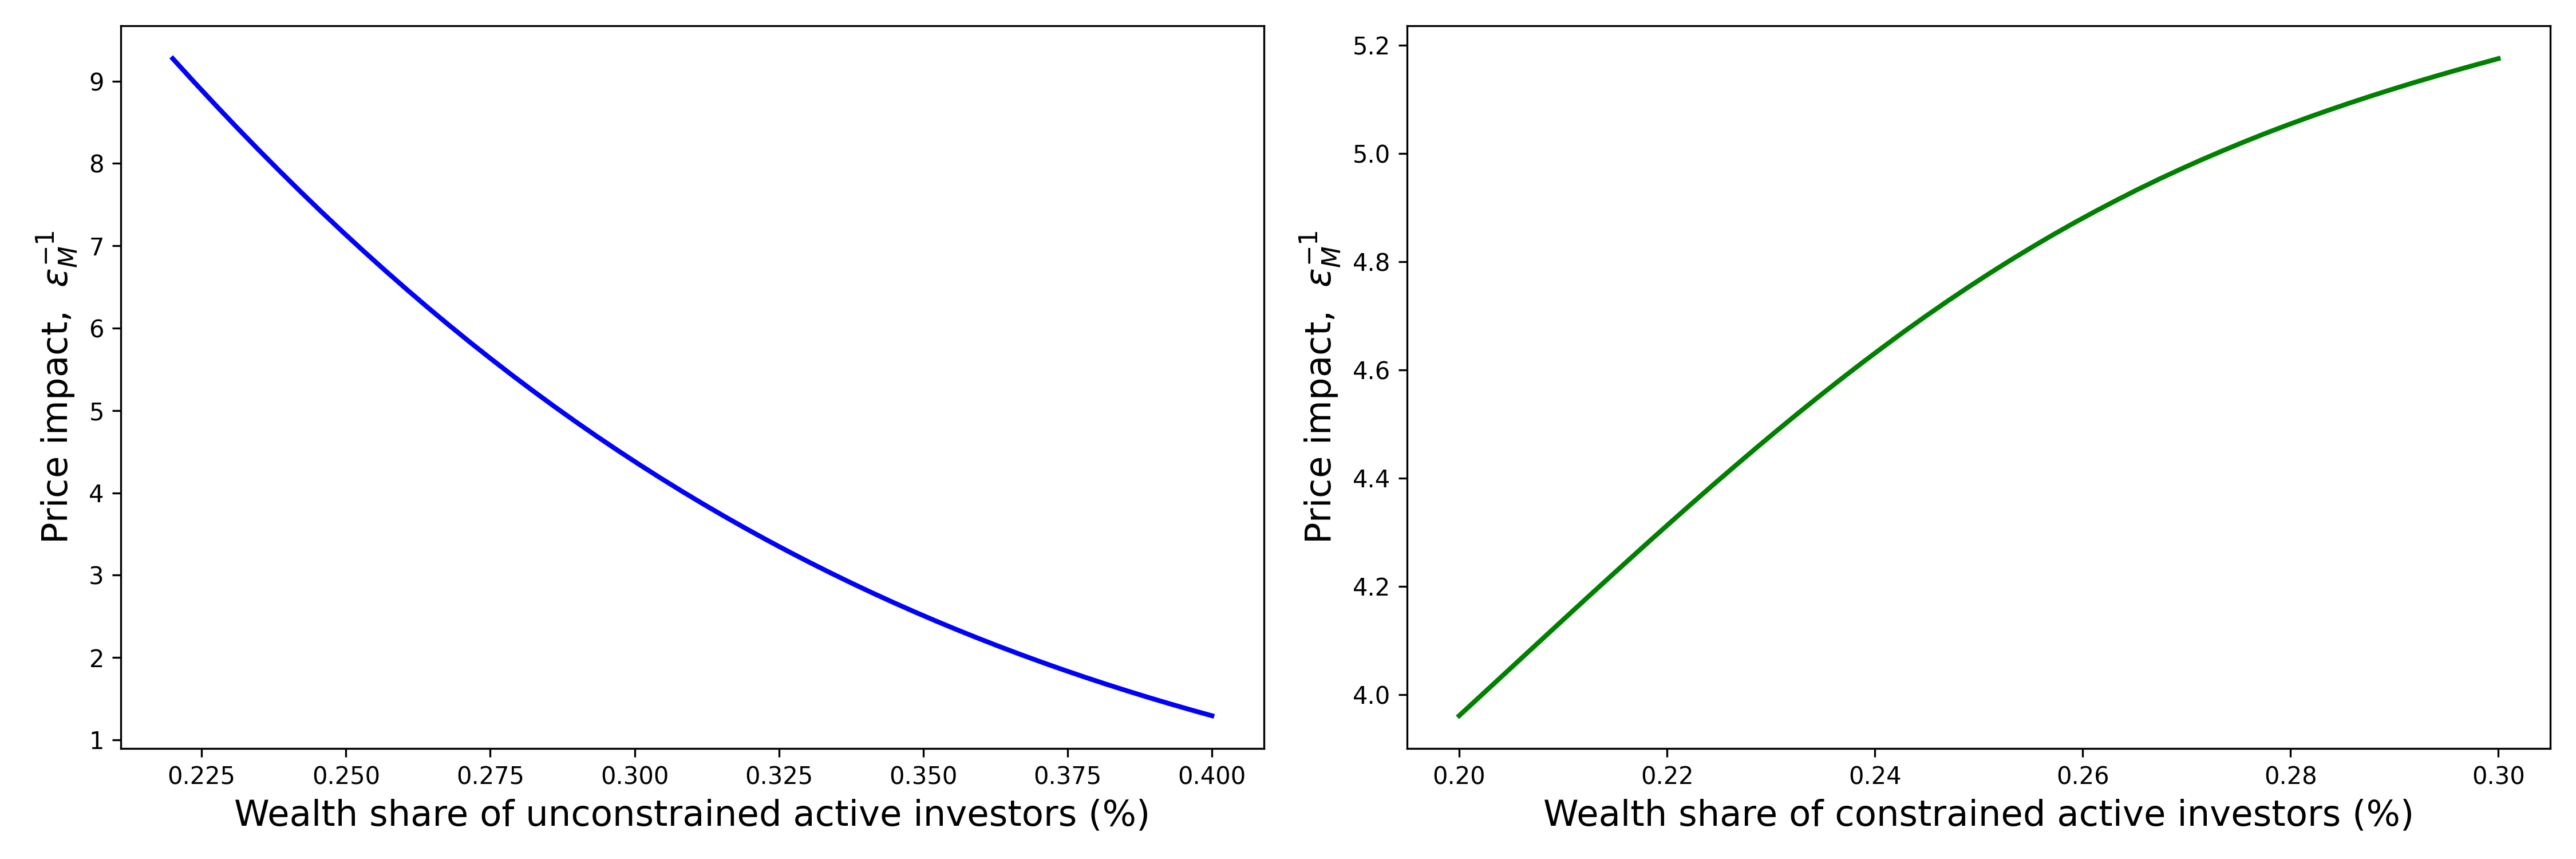
\includegraphics[width=0.95\linewidth]{figures/xu_xc_price_impact_off_equilibrium.png}
    \caption{\textbf{Conditional price impact.}\\
    Model-implied price impact of the dividend claim evaluated off the ergodic mean.
    In each panel, $\overline{\alpha}_{p,t}$ and $s_t$ are fixed at their unconditional means and one wealth-share coordinate is varied.
    Conditional price impact is computed as the change in $\log(P/D)$ per unit of passive-flow shock, where the shock is propagated one quarter forward through the state-variable dynamics.}
    \label{fig:price_impact_dynamic}
\end{figure}

\subsection{Return predictability and the variance of the price--dividend ratio}\label{sec:predictability}

We next examine the predictive relationship between the price--dividend ratio and future excess returns in the simulated economy.
Figure~\ref{fig:return_predictability} plots cumulative future excess returns against the current $P/D$ ratio, and Table~\ref{tab:return_predictability} reports the corresponding predictive-regression coefficient
\[
    \sum_{k=1}^{T} r_{t+k} - r_t = a + b\,(P/D)_t + \varepsilon_{t+T},\qquad T=4\text{ quarters},
\]
estimated both on the full sample and on the subsample of ``bad states'' in which $(P/D)_t$ lies below its $25$th percentile.
The slope is negative in both cases, and it is roughly $2.5$ times larger in magnitude in bad states.
This pattern is consistent with countercyclical risk premia: when the $P/D$ ratio is depressed, expected returns are high, and the $P/D$ ratio is correspondingly more informative about future returns.

\begin{figure}[!t]
    \centering
    
\includegraphics[width=0.6\linewidth]{figures/return_predictability.png}
    \caption{\textbf{Return predictability.}\\
    Scatter of cumulative future excess returns ($T=4$ quarters) against the current price--dividend ratio in the simulated baseline economy.
    Blue dots correspond to normal states and red dots to bad states defined as $(P/D)_t$ below the $25$th percentile of its long-run mean.
    Lines are the corresponding OLS fits.}\label{fig:return_predictability}
\end{figure}

Following \citet{campbell1988dividend} and \citet{cochrane2011presidential}, we decompose the unconditional variance of $pd_t \equiv \log(P/D)_t$ into a discount-rate component and a cash-flow component,
\begin{equation}\label{eq:cs_decomp}
    \var(pd_t) \;=\; \cov\!\left(pd_t,\; \sum_{k=1}^{\infty}\rho^{k-1}\Delta d_{t+k}\right) \;-\; \cov\!\left(pd_t,\; \sum_{k=1}^{\infty}\rho^{k-1} r_{t+k}\right).
\end{equation}
Dividing through by $\var(pd_t)$ yields the discount-rate share
\[
    \beta_r \;=\; -\,\frac{\cov\!\left(pd_t,\sum_{k=1}^{\infty}\rho^{k-1} r_{t+k}\right)}{\var(pd_t)},
\]
which we evaluate at a $40$-quarter horizon.
In the baseline economy $\beta_r = 1.16$, so essentially all of the variation in the $P/D$ ratio is driven by expected returns.
The cash-flow component actually \emph{offsets} rather than reinforces $pd_t$: because the dividend share is positively correlated with aggregate fundamentals, expected future dividend growth is higher precisely when $pd_t$ is low, producing a negative cash-flow covariance that mechanically pushes $\beta_r$ above one.

The counterfactuals show that this pattern comes from heterogeneity and frictions.
In the homogeneous, unconstrained economy $\beta_r = -0.02$, so variation in $pd_t$ reflects cash flows and not discount rates.
Removing only leverage constraints leaves $\beta_r = 1.24$, close to the baseline, so heterogeneous risk aversion alone is enough to deliver discount-rate-dominated variation in $pd_t$.
Setting $\overline{\alpha}=1$ yields $\beta_r = -0.21$: at this level passive demand would be optimal under homogeneous preferences with no frictions, so there are no state-dependent movements in the price of risk, and $pd_t$ again reflects cash flows.
The large $\beta_r$ in the baseline is thus a consequence of the frictions, not of the passive-demand process in isolation.
These magnitudes are in line with the empirical findings in \citet{cochrane2011presidential}, whose Table~II shows that $\beta_r$ exceeds unity for aggregate U.S. equities and that cash-flow news contributes little or nothing to the variance of $pd_t$.

The accounting identity in~\eqref{eq:cs_decomp} also connects the predictability of returns to the volatility of prices.
The ``excess volatility'' puzzle documented by \citet{shiller1981} and \citet{leroy1981present}, under which prices are too volatile to be justified by subsequent dividends, is mechanically the same fact as return predictability: if $\beta_r$ is close to one, then almost all of the observed variance of $pd_t$ must show up in predictable movements in future returns.
Our counterfactuals make this duality sharp.
Economies in which heterogeneity or leverage constraints bind simultaneously deliver large return volatility, a sizable price impact, and a predictive slope on $(P/D)_t$ close to the data, whereas the frictionless counterfactuals deliver low return volatility, a negligible price impact, and $\beta_r\approx 0$.
Matching the empirical excess-volatility and predictability facts therefore requires heterogeneity and frictions in the active sector, not just time variation in fundamentals or beliefs.

\begin{table}[!t]
\centering
\resizebox{0.65\textwidth}{!}{
    \begin{tabular}{@{}lcc@{}}
    \toprule
    Dependent variable: & \multicolumn{2}{c}{Cumulative excess return, $\sum_{k=1}^{4} r_{t+k}-r_t$} \\
    Sample: & Full & Bad state \\
    \midrule
    $(P/D)_t$ & $-0.05$ & $-0.12$ \\
              & $(0.0005)$ & $(0.0048)$ \\
    \midrule
    $R^2$        & $0.19$  & $0.06$  \\
    Observations & $79{,}120$ & $19{,}780$ \\
    \bottomrule
    \end{tabular}
    }
\vspace{2mm}
\captionsetup{font=footnotesize}
\caption{\textbf{Return predictability regression.}\\
This table reports OLS estimates of the predictive regression $\sum_{k=1}^{T} r_{t+k}-r_t = a + b\,(P/D)_t + \varepsilon_{t+T}$, where $T=4$ quarters, estimated on a $1{,}000$-year monthly simulation of the calibrated baseline economy.
Column~(1) uses the full sample.
Column~(2) restricts to ``bad states'' in which $(P/D)_t$ lies below the $25$th percentile of its long-run distribution.
Standard errors are in parentheses.}\label{tab:return_predictability}
\end{table}

\FloatBarrier

\subsection{Conditional price impact and dynamics}\label{sec:cond-price-impact}

Averaging across states masks the state dependence of aggregate elasticity emphasized in Section~\ref{sec:elasticity}.
To trace this dependence, we compute the model-implied \emph{conditional} price impact off the ergodic mean, plotted in Figure~\ref{fig:price_impact_dynamic}.
We fix passive demand $\overline{\alpha}_{p,t}$ and the dividend share $s_t$ at their unconditional means, vary one wealth-share coordinate at a time, and apply a fixed one-quarter passive-flow shock.
The shock is propagated through the dynamic transition of the state variables.
We then recompute $\log(P/D)$ at the shocked and unshocked states, and measure the conditional price impact as the resulting change in $\log(P/D)$ per unit of passive-flow shock.

The left panel of Figure~\ref{fig:price_impact_dynamic} shows that the price impact rises sharply as the wealth share of the unconstrained active sector $x_{u,t}$ falls.
When the sector most capable of absorbing risk is small, the market is less elastic and flow shocks translate into larger price movements.
The right panel shows that the price impact also rises monotonically in the wealth share of the constrained active sector $x_{c,t}$.
As more of the active sector hits its leverage limit, the residual risk-bearing capacity in $x_{u,t}$ shrinks and price impact grows.
These patterns mirror the analytical characterization in Proposition~\ref{prop_elasticity_pref_heterog} and explain why the conditional price impact reported in Table~\ref{tab:counterfactual_comparison} (the row labeled ``Cond.\ price impact ($D$)'' with a value of $8.50$) is substantially larger than its unconditional counterpart.

Combined with the counterfactual results, Figure~\ref{fig:price_impact_dynamic} makes clear that the very states in which risk-bearing capacity is depleted, with low $x_u$ or high $x_c$, are the states in which discount rates are most volatile and the $P/D$ ratio is most informative about future returns.
The large unconditional $\beta_r$ in Table~\ref{tab:counterfactual_comparison} is therefore driven by these tail states.

\subsection{Takeaways}\label{sec:takeaways}

The quantitative exercise delivers three main messages.
A calibration disciplined by sectoral FoF data and passive equity flows matches the level of the aggregate price impact, the volatility of dividend-claim returns, and the level of the risk premium.
Preference heterogeneity is quantitatively central: it alone accounts for roughly three-quarters of the baseline price impact and produces a discount-rate-dominated variance decomposition of the $P/D$ ratio, even when leverage constraints are slack.
Leverage constraints and a below-efficient passive share are complementary amplifiers that operate through state-dependent risk sharing.
Finally, the excess-volatility puzzle and return predictability are two sides of the same coin in our economy.
The same frictions that raise aggregate price impact are the ones that push $\beta_r$ above one, consistent with \citet{cochrane2011presidential}, and counterfactuals that eliminate heterogeneity or shift $\overline{\alpha}$ to its optimum under homogeneous preferences collapse all three facts at once.



% \section{Conclusion}
% This paper provides an analysis of the determinants of aggregate market elasticity in a general equilibrium framework with rich investor heterogeneity, passive investment, and financial constraints. Our analysis yields several important insights about market inelasticity and its implications for asset prices and market volatility.

% A central finding of our work is the crucial role of cross-price elasticity--the sensitivity of demand for risky assets to changes in interest rates. When cross-elasticity is zero, aggregate market elasticity is simply an average of individual investors' price elasticities, consistent with partial equilibrium intuition. However, with non-zero cross-elasticity, the market can be infinitely elastic even when individual investors are highly inelastic, as changes in interest rates offset movements in risk premia. This highlights how general equilibrium effects fundamentally alter the relationship between individual and aggregate elasticities.

% We show that beyond cross-elasticity effects, the key determinant of market elasticity is how risk is allocated in the economy. When passive investors hold an efficient share of risky assets, the market remains infinitely elastic regardless of individual investor preferences. However, when risk is misallocated, portfolio flows have meaningful price impacts.

% Our model demonstrates that market elasticity is both state-dependent and time-varying, influenced by the distribution of wealth between active and passive investors as well as the allocation of wealth among active investors themselves. While passive investment and leverage constraints amplify the price impact of flows, preference heterogeneity can make markets more elastic by improving risk allocation. These findings highlight that market inelasticity serves as an indicator of underlying inefficiencies in risk allocation rather than a fundamental feature of markets.

% The framework developed here helps explain several empirical patterns, including the countercyclical nature of the volatility multiplier and the relationship between passive investment growth and market dynamics. It also provides a foundation for analyzing how different market frictions interact to influence aggregate elasticity and market stability. Our results suggest that policies aimed at improving risk allocation may be more effective at reducing excess volatility than those focused on individual investor behavior.

% Future research could extend this framework to study the implications of market inelasticity for asset pricing anomalies, monetary policy transmission, and financial stability. The role of market structure and trading mechanisms in determining aggregate elasticity also remains an important area for investigation.

\section{Conclusion}

This paper develops a general equilibrium model with heterogeneous investors, passive demand, and financial constraints to study the determinants of aggregate market elasticity. We show how general equilibrium adjustments, particularly the joint movement of the risk-free rate and the risk premium, fundamentally shape the price impact of portfolio flows.  

A central insight is the role of cross-price elasticity. When demand for risky assets responds to interest rates, shifts in the risk premium are offset by changes in the risk-free rate. In this case, the market can be infinitely elastic even if individual investors are highly inelastic. Aggregate elasticity becomes finite only when risk is initially misallocated: portfolio flows then alter aggregate savings behavior, preventing interest rates from fully offsetting risk-premium movements.  

Macro elasticity is both state-dependent and time-varying. Passive investors amplify price impacts, leverage constraints further tighten risk-bearing capacity, while preference heterogeneity increases elasticity by improving risk allocation. Inelasticity alone does not generate excess volatility, nor do flows in infinitely elastic markets; both elements are needed to explain observed fluctuations and the countercyclical volatility multiplier.  

Our analytical results rely on a state-global perturbation method that provides closed-form characterizations of elasticity, while our quantitative analysis solves the full dynamic model numerically. The calibrated model highlights how the wealth distribution across households, intermediaries, and long-term investors shapes aggregate elasticity and volatility.  

Overall, our findings suggest that market inelasticity is best understood as a symptom of inefficient risk allocation, rather than a structural feature of financial markets. Improving the allocation of risk across sectors may therefore be more effective for reducing excess volatility than targeting individual investor behavior. Future work could extend this framework to study asset pricing anomalies, monetary policy transmission, and the role of market structure in shaping aggregate elasticity.




\newpage
\singlespacing
\bibliographystyle{jf}
\phantomsection\addcontentsline{toc}{section}{\refname}
\clearpage
%{\small
\bibliography{references.bib}


\clearpage
\numberwithin{equation}{section}
\setcounter{table}{0}
\renewcommand{\thetable}{A.\arabic{table}}
\setcounter{figure}{0}
\renewcommand{\thefigure}{A.\arabic{figure}}
\setcounter{footnote}{0} 
% \renewcommand{\theprop}{A.\arabic{prop}}
% \setcounter{prop}{0}

\appendix
\onehalfspacing
% \newgeometry{left=1in,bottom=1in, top=1in, right=1in}
\part*{Appendix}\label{appendix}

\section{Derivations for Section \ref{sec:simple}}

\subsection{The bond demand view}

Define the normalized bond demand $b_{j} \equiv \frac{R_f^{-1} B_j}{W_j} = 1 -c_{j}(r,\pi) - \alpha_j (1-c_{j}(r,\pi))$ as the bond-to-wealth ratio:
\begin{equation}
    b_j = (1-\alpha_j) (1-c_j(r,\pi)) = 1-c_{j}(r,\pi) - \frac{P Q_j}{W_j}.
\end{equation}

Notice that the bond demand depends not only on the interest rate, but also on the price of the risky asset, that is, the cross-elasticity will generically be non-zero.

The market clearing condition for bonds can be expressed as follows
\begin{equation}
    \underbrace{x_a b_a}_{\textbf{active bond demand}} = \underbrace{- x_p b_p}_{\textbf{net bond supply}},
\end{equation}
where $x_j \equiv \frac{\omega_j W_{j}}{\omega_a W_a + \omega_p W_p} = \omega_j Q_{j,-1} $ denotes the wealth share of investor $j$.

Notice that $\frac{P Q_j}{W_j} = \frac{P}{Y+P} \frac{\omega_j Q_j}{x_j}$. 
We can then write the bond market-clearing condition as follows:
\begin{equation}
    1 - \overline{c}(\mu-p) -\frac{e^p}{1+e^p} \left[\omega_a Q_a + \omega_p Q_p\right] = 0 \iff
    \underbrace{\frac{1}{1+e^p} - \overline{c}(\mu-p)}_{\text{excess supply of goods}} -\frac{e^p}{1+e^p} \left[\omega_a Q_a + \omega_p Q_p-1\right] = 0
\end{equation}

The left-hand side of the two expressions above gives you total bond demand. 
In the partial equilibrium case, the risk premium adjusts to clear the market for risky assets, so $\omega_a Q_a + \omega_p Q_p=1$, keeping the interest rate fixed.
But, due to the cross-elasticity in bond demand, a change in the price of the risky asset --- keeping the interest rate fixed --- would create a disequilibrium in the bond market.
For instance, in the case $\chi_p \equiv - \overline{c}'(\mu-p) > 0$, a decrease in the price of the risky asset would create an insufficient demand for goods and an excess demand for bonds.
The excess demand for bonds would create an incentive to reduce the interest rate, 

% The $\hat{b}_j \equiv b_j - b_j^*$. Then, the linearized bond demand for the passive investor is given by
% \begin{equation}
%     \hat{b}_p = -(1-\alpha_p^*) \left[\frac{\partial c_p^*}{\partial r} \hat{r} + \frac{\partial c_p^*}{\partial \pi} \hat{\pi} \right] - (1-c_p^*) \overline{\alpha}_p^* \hat{\alpha}_p. 
% \end{equation}

% The linearized bond demand for the active investor is given by
% \begin{equation}
%     \hat{b}_a = -(1-\alpha_a^*) \left[\frac{\partial c_a^*}{\partial r} \hat{r} + \frac{\partial c_a^*}{\partial \pi} \hat{\pi} \right] - (1-c_a^*) \frac{\partial \alpha_a^*}{\partial \pi} \hat{\pi}.
% \end{equation}

% The risk premium is given by
% \begin{equation}
%     \hat{\pi} = - \hat{p} - \hat{r}.
% \end{equation}

% We can then write the bond demand as follows:
% \begin{equation}
%     \hat{b}_j = - \zeta_{}
% \end{equation}

% The linearized bond demand for a passive investor is given by
% \begin{equation}
%     b_j - b_j^* = \left[ r -r^* +\frac{c_j'(\mu-p^*)}{1-c_j(\mu-p^*)}   (p-p^*)\right] b_j^* - \alpha_j^* e^{r^*} (1-c_j(\mu-p^*))  \hat{\alpha}_j
% \end{equation}

% For simplicity, focus on the case $\overline{\alpha}_p = 1$, so $b^*_p = b_a^* = 0$.
% The passive bond demand is then given by
% \begin{equation}
%     x_p b_p=  f^b,
% \end{equation}
% where $f^b \equiv  -x_p [1-c_p(\mu-p^*)] \hat{\alpha}_p$.
% The active bond demand is given by
% \begin{equation}
%     x_a b_a  = -\zeta^b_p (p-p^*) - \zeta^b_r (r-r^*),
% \end{equation}
% where $\zeta^b_p = \zeta^b_r = -x_a g_a'(\mu-p^*-r^*)[1-c_a(\mu-p^*)]$.

% The demand system can be written as follows:
% \begin{equation}
%     \left[
%     \begin{matrix}
%         \zeta_p^q & \zeta^q_r\\
%         \zeta_p^b & \zeta^b_r 
%     \end{matrix}
%     \right] \left[ 
%     \begin{matrix}
%         p-p^*\\
%         r-r^*
%     \end{matrix}
%     \right] = \left[ 
%     \begin{matrix}
%         f^q\\
%     f^b
%     \end{matrix}
%     \right],
% \end{equation}
% where we denote here $f^q \equiv f$ for symmetry.

% Inverting the system above, we obtain
% \begin{equation}
%     \left[ 
%     \begin{matrix}
%         p-p^*\\
%         r-r^*
%     \end{matrix}
%     \right] = 
%     \frac{1}{\zeta_{p}^q \zeta^b_r - \zeta_r^q \zeta ^b_p } \left[
%     \begin{matrix}
%         \zeta^b_r  & -\zeta^q_r\\
%         -\zeta_p^b & \zeta_p^q
%     \end{matrix}
%     \right] 
%     \left[ 
%     \begin{matrix}
%         f^q\\
%     f^b
%     \end{matrix}
%     \right].
% \end{equation}

% The price is given by
% \begin{equation}
%     p-p^* = \frac{\zeta_r^b f^q - \zeta_r^q f^b}{\zeta_{p}^q \zeta^b_r - \zeta_r^q \zeta ^b_p } = 
%      x_p \hat{\alpha}_p\frac{\zeta_r^b  + \zeta_r^q (1-c_p(\mu-p^*))}{\zeta_{p}^q \zeta^b_r - \zeta_r^q \zeta ^b_p } = 0,
% \end{equation}
% using the fact that $\zeta^q_r = x_a g_a'(\mu-p^*-r^*)$ and $c_a(\mu-p^*) = c_p(\mu-p^*)$.

\section{Derivations for Section \ref{sec:model}}

\subsection{Investors' problem}

The Hamilton-Jacobi-Bellman (HJB) equation for investor $j$ can be written as
\begin{align}
    0 &= \max_{C_j, \alpha_j} f_j(C_j,V_j) + V_{j,W}\left[ r W_j + \pi^\top \alpha_j W_j  - C_j\right] +V_{j,X} \mu_X\nonumber\\
    &\qquad + \frac{1}{2} V_{j,WW} W_j^2 \|\sigma_j\|^2 + V_{j,WX}W_j \sigma_X \sigma_j^\top    + \frac{1}{2} \sum_{k=1}^3\ \sigma_{X,k}^\top V_{j,XX} \sigma_{X,k},
\end{align}
subject to 
\begin{equation}
    \alpha_j = \overline{\alpha}_p[ \alpha_{D,t}^m, \alpha_{B,t}^m, 0]^\top \qquad \text{for } j = 0, \qquad \qquad 
    \sigma_j \sigma_j^\top \leq \overline{\sigma}^2 \qquad \text{for } j = 2.
\end{equation}
given $\sigma_{j} = \alpha_j^\top \Sigma$, where $\alpha_{k,t}^m \equiv \frac{P_{k,t}}{P_{Y,t}}$ for $k \in \{D,B\}$.
For ease of notation, we dropped time subscripts.
Note that  $V_{j,X}$ and $V_{j,WX}$ are $1\times N$ vectors, $V_{j,XX}$ is a $N\times N$ matrix, and both $V_{j,W}$ and $V_{j,WW}$ are scalars.
The drift $\mu_X$ is a $N\times 1$ vector, the diffusion $\sigma_X$ is a $N\times 3$ matrix, while $\sigma_R$ is a $1\times 3$ vector.
The notation $\sigma_{X,k}$ denotes the $k-$th column of $\sigma_{X}$, that is, the exposure to the $k-$th Brownian motion.



The optimality condition for consumption and portfolio share are given by
\begin{align}
    f_{j,C}(C_j,V_j) &= V_{j,W}\\
    V_{j,W} \pi &= - V_{j,WW} W_j \Sigma \Sigma^\top \alpha_j -  \Sigma (V_{j,WX} \sigma_X)^\top + \tilde{\nu}_{j,t} \Sigma \Sigma^\top \alpha_{j}.
\end{align}
where the second optimality condition holds for $j = 1,2$, and $\tilde{\nu}_{j,t}$ is the Lagrange multiplier on the leverage constraint. 

The optimal consumption is given by
\begin{equation}
 C_j = \rho^\psi ((1-\gamma_j) V_j)^{\frac{1-\gamma_j\psi }{1-\gamma_j}}V_{j,W}^{-\psi}.
\end{equation}

The optimal portfolio share for an active investor is given by
\begin{equation}
\sigma_j =  -\frac{V_{j,W}}{V_{j,WW} W_j + \tilde{\nu}_{j,t}}  \eta_j   - \frac{V_{j,WX}}{V_{j,WW} W_j + \tilde{\nu}_{j,t}} \sigma_X.
\end{equation}
using the fact that $\pi = \Sigma \eta^\top$.

Given the homotheticity of preferences, the value function for investor $j$ can be written as
\begin{equation}\label{app:value_function}
    V_{j,t} = \left(\frac{c_{j,t}}{\rho^\psi}\right)^{\frac{1-\gamma_j}{1-\psi}} \frac{W_{j,t}^{1-\gamma_j}}{1-\gamma_j}.
\end{equation}

This particular parametrization of the value function implies that the consumption-wealth ratio is given by
\begin{equation}
    \frac{C_{j,t}}{W_{j,t}} = c_{j,t}.
\end{equation}

The optimal risk exposure for active investors is given by
\begin{equation}
    \sigma_{j,t}
    =\frac{1}{1+\nu_{j,t}} \left[ \frac{\eta_t}{\gamma_j}  + \frac{1-\gamma_j^{-1}}{\psi-1} \sigma_{c_j,t} \right],
\end{equation}
where $\nu_{j,t} \equiv \tilde{\nu}_{j,t} / (V_{j,WW,t} W_{j,t})$ is the normalized Lagrange multiplier on the leverage constraint.

Plugging the consumption-wealth ratio into the HJB equation and using Equation \eqref{app:value_function}, we obtain
\begin{align}
        0 &=  \frac{\rho   }{1-\psi^{-1}} \left[  \rho^{-1} c_j-1 \right] + r  + \eta \sigma_j^ \top   - c_j + \frac{1}{1-\psi} \left[ \frac{\xi_{j,X}}{\xi_j} \mu_X + \frac{1}{2} \sum_{k=1}^d \sigma_{X,k}^\top \frac{\xi_{j,XX}}{\xi_j} \sigma_{X,k}\right]\nonumber\\
    &\qquad - \frac{\gamma_j}{2} \| \sigma_j\|^2  + \frac{1-\gamma_j}{1-\psi} \frac{c_{j,X}}{c_j} \sigma_X  \sigma_j^ \top    + \frac{1}{2} \frac{\psi-\gamma_j}{(1-\psi)^2} \sum_{k=1}^d \sigma_{X,k}^\top \frac{c_{j,X}^\top}{c_j} \frac{c_{j,X}}{c_j} \sigma_{X,k}.
\end{align}

Rearranging the expression above, we obtain
\begin{small}
\begin{equation}
    c_{j,t} = \psi \rho + (1-\psi) \left[ r_t + \eta_t \sigma_{j,t}^\top - \frac{\gamma_j}{2} \| \sigma_{j,t}\|^2 \right] + \mu_{c_j,t} + (1-\gamma_j)  \sigma_{c_j,t} \sigma_{j,t}^\top + \frac{\psi - \gamma_j}{1-\psi} \frac{\|\sigma_{c_j,t} \|^2}{2},
\end{equation}
\end{small}
where the law of motion of $c_{j,t}$ is given by
\begin{equation}
    \frac{d c_{j,t}}{c_{j,t}} = \mu_{c_j,t} dt + \sigma_{c_j,t} d Z_t,
\end{equation}
and the drift and diffusion of $c_{j,t}$ are given by Ito's lemma:
\begin{align}
    \mu_{c_j,t} &= \frac{c_{j,X}}{c_j} \mu_{X,t} + \frac{1}{2} \sum_{k=1}^d \sigma_{X,k,t}^\top \frac{c_{j,XX,t}}{c_{j,t}} \sigma_{X,k,t}, \qquad \qquad 
    \sigma_{c_j,t} = \frac{c_{j,X}}{c_j} \sigma_{X,t}.
\end{align}


\subsection{Pricing condition}

Let $p_{D,t} = \frac{P_{D,t}}{Y_t}$ and $p_{B,t} = \frac{P_{B,t}}{Y_t}$ denote the normalized prices of the dividend and bond claims, respectively.
The normalized price of the aggregate claim is $p_{Y,t} = \frac{P_{Y,t}}{Y_t}$.
The pricing condition for asset $k \in\{D,B\}$ is given by
\begin{equation}
    r_t + \sigma_{R_k,t} \eta_t^\top = \frac{1}{p_{k,t}} + \mu + \mu_{p_k,t} + \sigma \sigma_{p_k,t}^\top,
\end{equation}
where $\sigma_{R,t} = \sigma + \sigma_{p_k,t}$ and $(\mu_{p_k,t}, \sigma_{p_k,t})$ are given by Ito's lemma:
\begin{equation}
    \mu_{p_k,t} = \frac{p_{k,X,t}}{p_{k,t}} \mu_{X,t} + \frac{1}{2}\sum_{k=1}^d \sigma_{X,k,t}^\top\,\frac{p_{k,XX,t}}{p_{k,t}}\,\sigma_{X,k,t}, \qquad \qquad 
    \sigma_{p_k,t} = \frac{p_{k,X,t}}{p_{k,t}} \sigma_{X,t}.
\end{equation}

The expected return and risk exposure on the aggregate claim are given by
 $\mu_{R_Y,t} = \alpha_{D,t}^m \mu_{R_D,t} + \alpha_{B,t}^m \mu_{R_B,t}$ and $\sigma_{R_Y,t} = \alpha_{D,t}^m \sigma_{R_D,t} + \alpha_{B,t}^m \sigma_{R_B,t}$, respectively.

% Let $y_t \equiv Y_t/P_t$ denote the dividend yield on the risky asset.
% From Equation~\eqref{eq:risky-asset-ret}, we can write the expected return on the risky asset as:
% \begin{equation}
%     r_t + \theta_t \| \sigma_{R,t}\| = y_t + \frac{1}{dt} \frac{d(Y_t/y_t)}{(Y_t/y_t)} = y_t + \mu - \mu_{y,t} + \|\sigma_{y,t}\|^2 - \sigma \sigma_{y,t}^\top.
% \end{equation}

% Rearranging the expression above, we obtain
% \begin{equation}\label{app:pricing_cond}
%     y_t = r_t + \theta_t \|\sigma_{R,t}\| -\mu + \mu_{y,t} - \|\sigma_{R,t}\|^2+ \sigma \sigma_{R,t}^\top,
% \end{equation}
% where $\sigma_{R,t} = \sigma - \sigma_{y,t}$ and $(\mu_{y,t}, \sigma_{y,t})$ are given by Ito's lemma:
% \begin{equation}
%     \mu_{y,t} = y_{X,t} \mu_{X,t} + \frac{1}{2}\sum_{k=1}^d \sigma_{X,k,t}^\top\,y_{XX,t}\,\sigma_{X,k,t}, \qquad \qquad 
%     \sigma_{y,t} = y_{X,t} \sigma_{X,t}.
% \end{equation}

\subsection{Aggregate state variable}

Define the share of wealth of type-$j$ investors as follows
\begin{equation}
    x_{j,t} \equiv \frac{\omega_j W_{j,t}}{\sum_{i=0}^2 \omega_i W_{i,t}}.
\end{equation}


We define the aggregate state variable as $X_t = (x_{1,t}, x_{2,t}, \overline{\alpha}_{p,t}, s_t)$.

\paragraph{Market clearing conditions.}
We can write the market clearing condition for the equity claim, corporate bond claim, and short-term bonds as follows:
\begin{equation}
    \sum_{j=0}^2 \omega_j W_{j,t} \alpha_{j,k,t} = P_{k,t}, \qquad 
    \sum_{j=0}^2 \omega_j W_{j,t} (1-\alpha_{j,D,t}-\alpha_{j,B,t}) = 0,
\end{equation}
for $k \in \{D,B\}$.

Using the fact that $P_{Y,t} = P_{D,t} + P_{B,t}$, we obtain:
\begin{equation}
    \sum_{j=0}^2 \omega_j W_{j,t} = P_{Y,t}.
\end{equation}

The market clearing condition for goods is given by
\begin{equation}
    \sum_{j=0}^2 x_{j,t} c_{j,t} = \frac{1}{p_{Y,t}}.
\end{equation}

We can then write the market clearing condition for the equity claim, corporate bond claim, and the derivative as follows:
\begin{equation}
    \sum_{j=0}^2 x_{j,t} \alpha_{j,D,t} = \alpha_{D,t}^m, \qquad 
    \sum_{j=0}^2 x_{j,t} \alpha_{j,B,t} = \alpha_{B,t}^m, \qquad 
    \sum_{j=0}^2 x_{j,t} \alpha_{j,F,t} = 0.
\end{equation}  

Let $\alpha_t^m = [\alpha_{D,t}^m, \alpha_{B,t}^m,0]^\top$ denote the market weights of the dividend, bond, and derivative claims.
We can then write the market clearing conditions above in a compact way:
\begin{equation}
    \sum_{j=0}^2 x_{j,t} \alpha_{j,t} = \alpha_t^m.
\end{equation}
Multiplying both sides by $\Sigma$ and using the fact that $\sigma_{R_Y,t} = \omega_{D,t} \sigma_{R_D,t} + \omega_{B,t} \sigma_{R_B,t}$, we obtain
\begin{equation}
    \sum_{j=0}^2 x_{j,t} \sigma_{j,t} = \sigma_{R_Y,t}.
\end{equation}

\paragraph{Law of motion of the aggregate state variable.}
The law of motion of $\overline{\alpha}_{p,t}$ is given by \eqref{eq:alpha_p_process}.
The law of motion of $s_t$ is given by \eqref{eq:s_process}.
To compute the law of motion of $x_{j,t}$, first, note that the law of motion of wealth for a type-$j$ investor can be written as
\begin{equation}
    \frac{d W_{j,t}}{W_{j,t}} = \left[ r_t + \eta_t \sigma_{j,t}^\top - c_{j,t} \right]dt + \sigma_{j,t} d Z_t.
\end{equation}

From Ito's lemma, the law of motion of $x_{j,t}$ is given by
\begin{align*}
    \frac{dx_{j,t}}{x_{j,t}} 
    &= \Big[ r_t + \pi_t^\top \alpha_{j,t} - c_{j,t} - \mu_{P_Y,t} 
        - (\sigma_{j,t} - \sigma_{R_Y,t}) \, \sigma_{R_Y,t}^\top 
        + \kappa \frac{\omega_j - x_{j,t}}{x_{j,t}} \Big] dt  
        + (\sigma_{j,t} - \sigma_{R_Y,t}) \, dZ_t.
\end{align*}
using $\mu_{P_Y,t} = \mu_{R_Y,t} - \mu_{R_D,t} \alpha_{D,t}^m - \mu_{R_B,t} \alpha_{B,t}^m$.


\subsection{Block recursivity and the mutual fund theorem}

To compute the equilibrium, one needs to solve a system of $5$ partial differential equations (PDEs), involving the three consumption-wealth ratios $\{c_{j,t}(X_t)\}_{j=0}^2$ and the two price-dividend ratios $\{p_{k,t}(X_t)\}_{k=D,B}$. %$\xi_{j}(x,\overline{\alpha}_p)$
These functions depend on $4$ state variables, the $2-$dimensional vector $x_{t}$, the portfolio share of passive investors $\overline{\alpha}_{p,t}$, and the dividend share $s_t$.

The system of PDEs satisfies an important \textit{block-recursive} structure.
We can first solve for a reduced system of PDEs involving $(c_j,p_Y)$ in the set of states $\hat{X}_t = (x_{1,t}, x_{2,t}, \overline{\alpha}_{p,t})$.
Given the solution of the reduced system of PDEs, we can then solve for $p_{D,t}$ and $p_{B,t}$ in the full set of states $X_t = (x_{1,t}, x_{2,t}, \overline{\alpha}_{p,t}, s_t)$.

\subsubsection{Block recursivity}

We next derive the system of PDEs. 
We will show that one can solve for a reduced system of PDEs involving $(c_j,p_Y)$.
% This requires expressing all equilibrium quantities as functions of the aggregate state variables $X_t$ and the functions $(c_j,p_Y)$ and their derivatives.
This is the crucial in the obtaining the mutual fund theorem in our setting.

\begin{lemma}\label{lemma:block_recursivity}
    The consumption-wealth ratios, $\{c_{j,t}(X_t)\}_{j=0}^2$, and the price-dividend ratio for the aggregate claim, $p_Y(X_t)$, satisfy the following system of PDEs:
    \begin{align}
        c_{j,t} &= \psi \rho 
        + (1-\psi) \left[ r_t + \eta_{t}\,\sigma_{j,t}^\top - \frac{\gamma_j}{2} \|\sigma_{j,t}\|^2 \right] 
        +  \mu_{c_j,t} 
        + (1-\gamma_j) \sigma_{c_j,t} \sigma_{j,t}^\top 
        + \frac{\psi - \gamma_j}{1-\psi} \frac{\|\sigma_{c_j,t}\|^2}{2}\\
        \frac{1}{p_{Y,t}} &= r_t + \eta_{t}\,(\sigma + \sigma_{p_Y,t})^\top - \big(\mu + \mu_{p_Y,t} + \sigma \, \sigma_{p_Y,t}^\top\big),        
\end{align}
where $(r_t, \eta_t, \sigma_{j,t}, \mu_{c_j,t}, \sigma_{c_j,t}, \mu_{p_Y,t}, \sigma_{p_Y,t})$ are all functions of $X_t$, $(c_j,p_Y)$ and their derivatives.    
\end{lemma}

\begin{proof}
    We proceed in four steps. 
    First, we show how to solve for the diffusion of the endogenous state variables, $\sigma_{x_1,t}$ and $\sigma_{x_2,t}$, in terms of $X_t$, $(c_j,p_Y)$ and their derivatives.
    Second, we show how to solve for the drift of the endogenous state variables, $\mu_{x_1,t}$ and $\mu_{x_2,t}$, again in terms of $X_t$, $(c_j,p_Y)$ and their derivatives.
    Third, we show how to solve for the interest rate, $r_t$.
    Finally, we show how to obtain the PDEs for $(c_j,p_Y)$.

    In the derivations below, we drop the explicit dependence on $X$ for brevity.

    \paragraph{Step 1: Risk exposure of endogenous state variables.}
    Consider the expression for the risk exposure of the aggregate claim and the consumption-wealth ratio:
    \begin{align}
        \sigma_{R_Y} &= \sigma + \sum_{k=1}^2 \frac{p_{Y,x_k}}{p_{Y}} \sigma_{x_k} + \frac{p_{Y,\overline{\alpha}_p}}{p_{Y}} \sigma_{\overline{\alpha}_p} + \frac{p_{Y,s}}{p_{Y}} \sigma_{s},\\
        \sigma_{c_j} &= \sum_{k=1}^2 \frac{c_{j,x_k}}{c_{j}} \sigma_{x_k} + \frac{c_{j,\overline{\alpha}_p}}{c_{j}} \sigma_{\overline{\alpha}_p} + \frac{c_{j,s}}{c_{j}} \sigma_{s},
    \end{align}
    
    Notice that we can write $\sigma_{R_Y}$ as follows:
    \begin{equation}
        \sigma_{R_Y} = \chi_{\sigma_{R_Y},0} + \chi_{\sigma_{R_Y},1} \sigma_{x_1} + \chi_{\sigma_{R_Y},2} \sigma_{x_2},
    \end{equation}
    where the coefficients $\chi_{\sigma_{R_Y},k}$, $k=0,1,2$, are functions of $X$ given by 
    \begin{align}
        \chi_{\sigma_{R_Y},0} &= \sigma  +\frac{p_{Y,\overline{\alpha}_p}}{p_{Y}} \sigma_{\overline{\alpha}_p} + \frac{p_{Y,s}}{p_{Y}} \sigma_{s} ,\\
        \chi_{\sigma_{R_Y},k} &= \frac{p_{Y,x_k}}{p_{Y}}, k=1,2.
    \end{align}

    Similarly, we can write $\sigma_{c_j}$ as follows:
    \begin{equation}
        \sigma_{c_j} = \chi_{\sigma_{c_j},0} + \chi_{\sigma_{c_j},1} \sigma_{x_1} + \chi_{\sigma_{c_j},2} \sigma_{x_2},
    \end{equation}
    where the coefficients $\chi_{\sigma_{c_j},k}$, $k=0,1,2$, are functions of $X$ given by 
    \begin{align}
        \chi_{\sigma_{c_j},0} &= \frac{c_{j,\overline{\alpha}_p}}{c_{j}} \sigma_{\overline{\alpha}_p} + \frac{c_{j,s}}{c_{j}} \sigma_{s}\\
        \chi_{\sigma_{c_j},k} &= \frac{c_{j,x_k}}{c_{j}}, k=1,2.
    \end{align}

    The market price of risk 
    \begin{align}
        \eta &= \gamma_{a} \left[\chi_{a}\sigma_{R_Y} - \sum_{j=0}^2 x_{j} \frac{1-\gamma_j^{-1}}{\psi-1} \, \frac{\sigma_{c_j}}{1+\nu_{j}}\right],
    \end{align}
    where $\chi_{a} =\frac{1 - (1-x_{1}-x_{2}) \overline{\alpha}_{p}}{x_{1}+x_{2}}$ is a known function of the aggregate state variables $X$.
    
    We can then write $\eta$ as follows:
    \begin{equation}
        \eta = \chi_{\eta,0} + \chi_{\eta,1} \sigma_{x_1} + \chi_{\eta,2} \sigma_{x_2},
    \end{equation}
    where the coefficients $\chi_{\eta,k}$, $k=0,1,2$, are functions of $X$ given by 
    \begin{align}
        \chi_{\eta,k} &= \gamma_{a} \left[ \chi_{a}\chi_{\sigma_{R_Y},k} - \sum_{j=0}^2 x_{j} \frac{1-\gamma_j^{-1}}{\psi-1} \, \frac{\chi_{\sigma_{c_j},k}}{1+\nu_{j}}\right].
    \end{align}


    The risk exposure of investor $j = 0,1,2$ is given by
    \begin{align}
        \sigma_{0} &= \overline{\alpha}_{p} \sigma_{R_Y}\\
        \sigma_{j} &= \frac{1}{1+\nu_{j}} \left[ \frac{\eta}{\gamma_j} + \frac{1-\gamma_j^{-1}}{\psi-1} \, \sigma_{c_j} \right], \qquad j=1,2.
    \end{align}

    
    We can then solve for $\sigma_{j}$ in terms of the risk exposure of the endogenous state variables:
    \begin{equation}
        \sigma_{j} = \chi_{\sigma_j,0} + \chi_{\sigma_j,1} \sigma_{x_1} + \chi_{\sigma_j,2} \sigma_{x_2},
    \end{equation}
    where the coefficients $\chi_{\sigma_j,k}$, $k=0,1,2$, are functions of $X$ given by 
    \begin{align}
        \chi_{\sigma_0,k} &= \overline{\alpha}_{p} \chi_{\sigma_{R_Y},k}\\
        \chi_{\sigma_j,k} &= \frac{1}{1+\nu_{j}} \left[ \frac{\chi_{\eta,k}}{\gamma_j} + \frac{1-\gamma_j^{-1}}{\psi-1} \chi_{\sigma_{c_j},k} \right], \qquad j=1,2.
    \end{align}

    The risk exposure of the endogenous state variables is given by
    \begin{equation}
        \sigma_{x_j} = x_{j} \left[ \sigma_{j} -  \sum_{k=0}^2 x_{k} \sigma_{k}  \right],
    \end{equation}
    using the fact that $\sigma_{R_Y} = \sum_{k=0}^2 x_{k} \sigma_{k}$.
    
    This gives us a system of equations determining $\sigma_{x_j,t}$:\small
    \begin{equation}
            \begin{bmatrix}
                1 - x_{1} \sum_{k=0}^2 \left( \chi_{\sigma_1,1} - \chi_{\sigma_k,1} \right) x_{k} & - x_{1} \sum_{k=0}^2 \left( \chi_{\sigma_1,2} - \chi_{\sigma_k,2} \right) x_{k}\\
                - x_{2} \sum_{k=0}^2 \left( \chi_{\sigma_2,1} - \chi_{\sigma_k,1} \right) x_{k} & 1 - x_{2} \sum_{k=0}^2 \left( \chi_{\sigma_2,2} - \chi_{\sigma_k,2} \right) x_{k}
            \end{bmatrix}
            \begin{bmatrix}
                \sigma_{x_1}\\
                \sigma_{x_2}
            \end{bmatrix}
            =
            \begin{bmatrix}
              x_{1} \sum_{k=0}^2 \left( \chi_{\sigma_1,0} - \chi_{\sigma_k,0} \right) x_{k} \\
              x_{2} \sum_{k=0}^2 \left( \chi_{\sigma_2,0} - \chi_{\sigma_k,0} \right) x_{k}
            \end{bmatrix}.
    \end{equation}\normalsize
    
    Solving the system above, we obtain $\sigma_{x_j}$ as a function of $X$ and the functions $c_j$ and $p_{Y}$ and their derivatives.
    Given $\sigma_{x_j}$, we can solve for $\sigma_{j},$ $\eta$, $\sigma_{c_j}$, and $\sigma_{R_Y}$ using the expressions above. 
    The risk premium on the aggregate claim is given by $\pi_{Y} = \sigma_{R_Y} \eta^\top$.

    \paragraph{Step 2: Drift of endogenous state variables.} 
Given $(\sigma_j, \eta, \sigma_{R_Y})$, we can solve for the drift of the endogenous state variables:
\begin{align}
    \mu_{x_j} &= x_{j} \left[ 
        (\eta-\sigma_{R_Y}) \left( \sigma_{j} -\sigma_{R_Y} \right)^\top - \left( c_{j} - \frac{1}{p_{Y}}  \right)
     \right] + \kappa (\omega_j - x_{j}),
\end{align}

This gives us $\mu_{X}$ and $\sigma_{X}$ in terms of $X$, $(c_j,p_Y)$ and their derivatives.
We can then solve for the drift of $c_j$ and $p_{Y}$ using Ito's lemma:
\begin{align}
    \mu_{c_j} &= \frac{c_{j,X}}{c_{j}} \mu_{X} + \frac{1}{2}\sum_{k=1}^3 \sigma_{X,k}^\top\,\frac{c_{j,XX}}{c_{j}}\,\sigma_{X,k},\\
    \mu_{p_Y} &= \frac{p_{Y,X}}{p_{Y}} \mu_{X} + \frac{1}{2}\sum_{k=1}^3 \sigma_{X,k}^\top\,\frac{p_{Y,XX}}{p_{Y}}\,\sigma_{X,k}.
\end{align}

\paragraph{Step 3: Interest rate.}
Given the expressions derived in the previous steps, we can solve for the shifter of the consumption-wealth ratio $\xi_{j,t}$:
\begin{equation}
    \xi_{j} = \mu_{c_j} 
    + (1-\gamma_j) \sigma_{c_j} \sigma_{j}^\top 
    + \frac{\psi - \gamma_j}{1-\psi} \frac{\|\sigma_{c_j}\|^2}{2}.
\end{equation}

We can then solve for $\xi = \sum_{j=0}^2 x_{j} \xi_{j}$ and the interest rate:
\begin{align}
    r &= \rho 
    + \psi^{-1} \left(\mu_{p_Y} + \mu + \sigma \sigma_{p_Y}^\top + \xi \right)
    + (1-\psi^{-1}) \sum_{j=0}^2 x_{j} 
        \frac{\gamma_j }{2} \|\sigma_{j}\|^2
    - \pi_{Y}.
\end{align}

\paragraph{Step 4: PDEs for the consumption-wealth ratio and price-dividend ratio.}
From the expression for the consumption-wealth ratio and the pricing condition for the aggregate claim, we can write the PDE for $c_j$ and $p_Y$ as follows:
\begin{align}
        c_{j} &= \psi \rho 
        + (1-\psi) \left[ r + \eta\,\sigma_{j}^\top - \frac{\gamma_j}{2} \|\sigma_{j}\|^2 \right] 
        +  \mu_{c_j} 
        + (1-\gamma_j) \sigma_{c_j} \sigma_{j}^\top 
        + \frac{\psi - \gamma_j}{1-\psi} \frac{\|\sigma_{c_j}\|^2}{2}\\
        \frac{1}{p_{Y}} &= r + \eta\,\sigma_{R_Y}^\top - \big(\mu + \mu_{p_Y} + \sigma \, \sigma_{p_Y}^\top\big),        
\end{align}
Notice that $(r, \eta, \sigma_{j}, \mu_{c_j}, \sigma_{c_j}, \mu_{p_Y}, \sigma_{p_Y})$ are all functions of $X$, $(c_j,p_Y)$ and their derivatives.
Hence, these equations form a system of PDEs for $(c_j,p_Y)$.
\end{proof}

A corollary of the above proposition is that the consumption-wealth ratio and price-dividend ratio are independent of the dividend share $s$.
\begin{cor}
    The consumption-wealth ratio $c_j$ and price-dividend ratio $p_Y$ are a function of the reduced state vector $\hat{X} = (x_1,x_2,\overline{\alpha}_p)$.
\end{cor}
\begin{proof}
    The dividend share $s$ does not appear in the expressions for PDE system for $(c_j,p_Y)$.
    They only appear indirectly through $\mu_{s}$ and $\sigma_{s}$.
    If $(c_j,p_Y)$ are a function of $\hat{X}$, then their derivatives with respect to $s$ are zero, and $s$ completely drops out of the PDE system for $(c_j,p_Y)$.
\end{proof}

\subsubsection{The mutual fund theorem}

Lemma~\ref{lemma:block_recursivity} and its corollary show that the consumption-wealth ratio and price-dividend ratio of the aggregate claim are independent of the dividend share $s$.
This implies that investor's consumption or wealth choices are not exposed to idiosyncratic dividend-share shocks:
\begin{equation}
    \sigma_{j,t,3} = \sigma_{R_Y,t,3} = \sigma_{R_F,t,3} = 0,
\end{equation}
where the third component of the risk exposure vector is the dividend-share shock.

We can implement the risk exposure $\sigma_{j,t}$ by holding the market index fund and a derivative.
Let $\hat{\sigma}_{j,t} = [\sigma_{j,t,1}, \sigma_{j,t,2}]$, $\hat{\Sigma}_{t} = \left[\begin{matrix}
 \hat{\sigma}_{R_Y,t} \\
 \hat{\sigma}_{R_F,t}
\end{matrix}\right]$, and $\hat{\alpha}_{j,t} = [\alpha_{j,Y,t}, \alpha_{j,F,t}]^\top$, then we can define the portfolio shares of the market index fund and the derivative as:
\begin{equation}
    \hat{\sigma}_{j,t} = \hat{\alpha}_{j,t}^\top \hat{\Sigma}_{t} \Rightarrow \hat{\alpha}_{j,t}^\top = \hat{\sigma}_{j,t} \hat{\Sigma}_{t}^{-1}.
\end{equation}

We can then write the risk exposure $\sigma_{j,t}$ as:
\begin{equation}
    \sigma_{j,t} = \alpha_{j,Y,t} \sigma_{R_Y,t} + \alpha_{j,F,t} \sigma_{R_F,t}.
\end{equation}
Using the fact that $\sigma_{R_Y,t} = \frac{P_{D,t}}{P_{Y,t}} \sigma_{R_D,t} + \frac{P_{B,t}}{P_{Y,t}} \sigma_{R_B,t}$, we obtain:
\begin{equation}
    \sigma_{j,t} = \alpha_{j,Y,t} \frac{P_{D,t}}{P_{Y,t}} \sigma_{R_D,t} + \alpha_{j,Y,t} \frac{P_{B,t}}{P_{Y,t}} \sigma_{R_B,t} + \alpha_{j,F,t} \left( \frac{P_{B,t}}{P_{Y,t}} \sigma_{R_Y,t} + \frac{P_{D,t}}{P_{Y,t}} \sigma_{R_D,t} \right).
\end{equation}
Hence, this implies that the portfolio shares of dividend and bond claims are given by:
\begin{equation}
    \alpha_{j,D,t} = \alpha_{j,Y,t} \frac{P_{D,t}}{P_{Y,t}},
    \quad
    \alpha_{j,B,t} = \alpha_{j,Y,t} \frac{P_{B,t}}{P_{Y,t}},
\end{equation}
where $\alpha_{j,Y,t}$ is the portfolio share of the market index fund defined.

\paragraph{Pricing the individual claims.} The normalized price of the dividend claim satisfies the pricing condition:
\begin{equation}
    \frac{s_t}{p_{D,t}} = r_t + \sigma_{R_D,t} \eta_t^\top - \big(\mu + \mu_{p_D,t} + \sigma \, \sigma_{p_D,t}^\top\big),
\end{equation}
where
\begin{equation}
    \mu_{p_{D,t}} = \frac{p_{D,X,t}}{p_{D,t}} \mu_{X,t} + \frac{1}{2}\sum_{k=1}^3 \sigma_{X,k,t}^\top\,\frac{p_{D,XX,t}}{p_{D,t}}\,\sigma_{X,k,t}, \qquad \qquad 
    \sigma_{p_{D,t}} = \frac{p_{D,X,t}}{p_{D,t}} \sigma_{X,t}.
\end{equation}

% \paragraph{Mapping to \citet{MenzlySantosVeronesi2004}.} We can map the dividend share $s$ to notation in \citet{MenzlySantosVeronesi2004} as follows:
% \begin{equation}
%     \sigma_s = v^1- v^0, \qquad (1-\overline{s}) v^0 + \overline{s} v^1 = 0,
% \end{equation}
% which implies that
% \begin{equation}
%     v^0 + \overline{s} (v^1- v^0) = 0 \Rightarrow v^0 = - \overline{s} \sigma_s, \qquad v^1 = (1-\overline{s}) \sigma_s,
% \end{equation}
% \begin{equation}
%     v^1 - s^ 1 v^ 1 - (1-s^1)v^0 = v^1- v^0 - s^ 1 (v^1- v^0) = (1-s^1)(v^1- v^0)
% \end{equation}
% \begin{equation}
%     v^0 - s^ 1 v^ 1 - (1-s^1)v^0 = v^0- v^0 - s^ 1 (v^1- v^0)= -s^ 1 (v^1- v^0)
% \end{equation}

\section{Derivations for Section \ref{sec:elasticity}: Perturbation Solution}\label{app:derivations-perturbation-solution}

In this section, we discuss the derivations of the perturbation solution in detail. 
Consistent with the block-recursivity property in Proposition~\ref{prop:mft}, the consumption-wealth ratios and the price-dividend ratio of the aggregate claim are independent of the dividend share $s$.

For these variables, we can focus on the reduced set of states $\hat{X} = (x, \overline{\alpha}_{p})$, where $x = (x_1, x_2)$ is the vector of wealth shares of the active investors. 
To price the individual claims, we need to consider the full set of states $X = (x, \overline{\alpha}_{p}, s)$.

The perturbation is defined by the following parameter restrictions:
\begin{equation}
    \gamma_j = \gamma (1+\hat{\gamma}_j \epsilon), \qquad 
    \overline{\sigma} = \|\sigma\| (1+\hat{\sigma} \epsilon), \qquad 
    \kappa = \hat{\kappa} \epsilon, 
\end{equation}
where $\sum_{j=0}^2 \omega_j \hat{\gamma}_j = 0$.

We also make assumptions about the dynamics of the exogenous state variables.
First, the portfolio share of passive investors is written as $\overline{\alpha}_{p} = 1 + \hat{\alpha}_{p} \epsilon$, where $\hat{\alpha}_{p}$ follows the process
\begin{equation}
d \overline{\alpha}_{p} = \kappa_p (\overline{\alpha} - \overline{\alpha}_{p}) dt + \sigma_p \epsilon dZ_t,
\end{equation}
where $\overline{\alpha} = 1+\hat{\alpha} \epsilon$.
Equivalently, $d\hat{\alpha}_{p} = \kappa_p(\hat{\alpha}-\hat{\alpha}_{p})dt + \sigma_p dZ_t$.

Second, the dividend share is written as $s = \overline{s} + \hat{s} \epsilon$, where $\hat{s}$ follows the process induced by
\begin{equation}
    d s = \kappa_s ( \overline{s} - s )dt + s (1-s) \sigma_s \epsilon d Z_t.
\end{equation} 

The case $\epsilon = 0$ corresponds to the benchmark economy, in which there is no preference heterogeneity and the exogenous state variables are constant.
In particular, passive investors are fully invested in the risky asset and the dividend share is fixed at $s = \overline{s}$.


We expand the consumption-wealth ratio of investor $j\in\{0,1,2\}$ and the price-dividend ratio of the aggregate claim as follows:
\begin{align}
    c_{j}(x, \overline{\alpha}_p;\epsilon) &= c_{j,0}(x, \hat{\alpha}_p) + c_{j,1}(x, \hat{\alpha}_p) \epsilon+ c_{j,2}(x, \hat{\alpha}_p) \epsilon^2 + \mathcal{O}(\epsilon^3),\\
    p_{Y}(x, \overline{\alpha}_p;\epsilon) &= p_{Y,0}(x, \hat{\alpha}_p) + p_{Y,1}(x, \hat{\alpha}_p) \epsilon+ p_{Y,2}(x, \hat{\alpha}_p) \epsilon^2 + \mathcal{O}(\epsilon^3).
\end{align}

For each individual claim $k\in\{D,B\}$, we use the expansion
\begin{align}
    p_{k}(x, \overline{\alpha}_p, s;\epsilon) &= p_{k,0}(x, \hat{\alpha}_p, \hat{s}) + p_{k,1}(x, \hat{\alpha}_p, \hat{s}) \epsilon+ p_{k,2}(x, \hat{\alpha}_p, \hat{s}) \epsilon^2 + \mathcal{O}(\epsilon^3).
\end{align}

The following lemma summarizes some basic properties of the perturbation solution that will be useful for the derivations below.
\begin{lemma}[Basic properties of the perturbation solution]\label{lemma:basic_properties}
    The perturbation solution satisfies the following properties:
    \begin{enumerate}   
        \item The zeroth-order terms are constant:
        \begin{align}
            c_{j,0}(x, \hat{\alpha}_p) = c_{j}^*, \qquad 
            p_{Y,0}(x, \hat{\alpha}_p) = p_{Y}^*, \qquad 
            p_{k,0}(x, \hat{\alpha}_p, \hat{s}) = p_{k}^*, \qquad k \in \{D,B\},
        \end{align}
        for some constants $c_{j}^*, p_{Y}^*, p_{k}^*$ independent of $(x, \hat{\alpha}_p, \hat{s})$.
        \item The drift and diffusion of the state variables are first-order in $\epsilon$:
        \begin{align}
            \mu_{X} = \mathcal{O}(\epsilon), \qquad 
            \sigma_{X} = \mathcal{O}(\epsilon).
        \end{align}
        \item The first-order and second-order corrections to the consumption-wealth ratio and the price-dividend ratio for the aggregate claim can be written as:\small
        \begin{align}
            c_{j,1}(x, \hat{\alpha}_p) &= \psi_{j,0}(x) + \psi_{j,\hat{\alpha}_p}(x) \hat{\alpha}_p, \qquad 
            c_{j,2}(x, \hat{\alpha}_p) = \Psi_{j,0}(x) + \Psi_{j,\hat{\alpha}_p}(x) \hat{\alpha}_p + \Psi_{j,\hat{\alpha}_p^2}(x) \hat{\alpha}_p^2, \\
            p_{Y,1}(x, \hat{\alpha}_p) &= \psi_{Y,0}(x) + \psi_{Y,\hat{\alpha}_p}(x) \hat{\alpha}_p, \qquad 
            p_{Y,2}(x, \hat{\alpha}_p) = \Psi_{Y,0}(x) + \Psi_{Y,\hat{\alpha}_p}(x) \hat{\alpha}_p + \Psi_{Y,\hat{\alpha}_p^2}(x) \hat{\alpha}_p^2,
        \end{align}\normalsize
        where $\psi_{j,l}(x)$ and $\Psi_{j,l}(x)$, for $j\in\{0,1,2,Y\}$ and $l\in\{0,\hat{\alpha}_p,\hat{\alpha}_p^2\}$, are functions of $x$.


        \item The first-order and second-order corrections to the price-dividend ratio for the individual claim can be written as:\small
        \begin{align}
            p_{k,1}(x, \hat{\alpha}_p, \hat{s}) &= \psi_{k,0}(x) + \psi_{k,\hat{\alpha}_p}(x) \hat{\alpha}_p + \psi_{k,\hat{s}}(x) \hat{s}, \\
            p_{k,2}(x, \hat{\alpha}_p, \hat{s}) &= \Psi_{k,0}(x) + \Psi_{k,\hat{\alpha}_p}(x) \hat{\alpha}_p + \Psi_{k,\hat{s}}(x) \hat{s} + \Psi_{k,\hat{\alpha}_p^2}(x) \hat{\alpha}_p^2 + \Psi_{k,\hat{\alpha}_p \hat{s}}(x) \hat{\alpha}_p \hat{s} + \Psi_{k,\hat{s}^2}(x) \hat{s}^2,
        \end{align}\normalsize
        where $\psi_{k,l}(x)$ and $\Psi_{k,l}(x)$, for $k\in\{D,B\}$ and $l\in\{0,\hat{\alpha}_p,\hat{\alpha}_p^2,\hat{s},\hat{\alpha}_p \hat{s},\hat{s}^2\}$, are functions of $x$.

        % \item The derivatives with respect to the state variables evaluated at $\epsilon = 0$ are given by:
        % \begin{align}
        %     \frac{\partial c_{j}}{\partial x} = 0_{1\times 2}, \qquad 
        %     \frac{\partial c_{j}}{\partial \overline{\alpha}_p} = \psi_{j,\hat{\alpha}_p}(x), \qquad 
        %     \frac{\partial p_{Y}}{\partial x} = 0_{1\times 2}, \qquad 
        %     \frac{\partial p_{Y}}{\partial \overline{\alpha}_p} = \psi_{Y,\hat{\alpha}_p}(x).
        % \end{align}
    \end{enumerate}
\end{lemma}

These properties follow from the definition of the perturbation solution.
When $\epsilon = 0$, the exogenous state variables are constant and investors have identical preferences.
Hence, the zeroth-order terms are independent of $(x,\hat{\alpha}_p,\hat{s})$.
The fact that the drift and diffusion of the state variables are first-order in $\epsilon$ comes from the assumptions on the dynamics of the exogenous state variables, and the fact that the zeroth-order terms are constant.
Properties 3 and 4 describe a solution that is global in the endogenous wealth shares and local in the exogenous state variables.

Our goal is to solve for the coefficients in this perturbation expansion.
We proceed in steps.
We first characterize the benchmark economy.
We then derive the first- and second-order corrections to the consumption-wealth ratios and the price-dividend ratio of the aggregate claim.
Finally, we derive the corresponding corrections to the price-dividend ratios of the individual claims.



\subsection{Proof of Lemma~\ref{lemma:benchmark}}\label{app:lemma1}

\begin{proof}
The assumption $\epsilon = 0$ implies that there is no preference heterogeneity and that passive investors are fully invested in the aggregate risky claim.
We guess and verify that, in this benchmark economy, expected returns are constant and the leverage constraint is slack.
In particular, the wealth distribution plays no role in equilibrium.
This implies that $\mu_{c_j,0}(X) = \mu_{p_Y,0}(X) = 0$ and $\sigma_{c_j,0}(X) = \sigma_{p_Y,0}(X) = 0_{1\times 3}$, where $0_{1\times 3}$ is a $1\times 3$ vector of zeros.

\paragraph{Risk exposure and market price of risk.}
The risk exposure vector for the aggregate claim is given by
\begin{equation}
    \sigma_{R_Y,0}(X) = \sigma.
\end{equation}
 
The market price of risk is therefore
\begin{equation}
    \eta_0(X) = \gamma \sigma,
\end{equation}
using the fact that $h_{a,t} = 0$ and $\chi_{a,t} = 1$.

The risk exposure of investor $j$ is therefore
\begin{equation}
    \sigma_{j,0}(X) = \sigma.
\end{equation}
Because $\overline{\sigma} = \|\sigma\|$, the leverage constraint is satisfied in the benchmark economy.

\paragraph{Risk premium and interest rate.}
The risk premium on the aggregate claim is given by
\begin{equation}
    \pi_{Y,0}(X) = \eta_0(X) \sigma_{R_Y,0}(X)^\top = \gamma \|\sigma\|^2,
\end{equation}
where $\|\sigma\|^2 = \sigma \sigma^\top$.

The interest rate is given by
\begin{align}
    r_0(X) &= \rho 
    + \psi^{-1} \mu 
    -(1+\psi^{-1}) 
        \frac{\gamma }{2} \|\sigma\|^2,
\end{align}
using the fact that $\xi_t = 0$, $\sigma_{j,t} = \sigma$, $\mu_{p_Y,t} = 0$, and $\sigma_{p_Y,t} = 0_{1\times 3}$ in the benchmark economy.

\paragraph{Consumption-wealth ratio and price-dividend ratio.}
The consumption-wealth ratio $c_{j,0}(X)$ is given by
\begin{align}
    c_{j,0}(X) &= \psi \rho 
    + (1-\psi) \left[ r_0(X) + \eta_0(X)\,\sigma^\top - \frac{\gamma}{2} \|\sigma\|^2 \right].
\end{align}

Plugging in the expression for $r_0(X)$ and $\eta_0(X)$, we obtain
\begin{equation}
    c_{j,0}(X) = \rho  - \left(1-\psi^{-1}\right)  \left( \mu - \frac{\gamma\|\sigma\|^2}{2} \right),
\end{equation}
We assume $\rho  > \left(1-\psi^{-1}\right)  \left( \mu - \frac{\gamma\|\sigma\|^2}{2} \right)$, so the benchmark consumption-wealth ratio is positive.

The goods-market-clearing condition then implies
\begin{equation}
    \frac{1}{p_{Y,0}(X)} = \rho  - \left(1-\psi^{-1}\right)  \left( \mu - \frac{\gamma\|\sigma\|^2}{2} \right).
\end{equation}

\paragraph{Drift and diffusion of wealth shares.}
The drift and diffusion of the wealth shares are given by
\begin{align}
    \mu_{x_j,0}(X) &= 0, \qquad
    \sigma_{x_j,0}(X) = 0_{1\times 3}, \qquad
    \forall j \in \{1,2\}.
\end{align}
using the fact that $\kappa = 0$, $\sigma_{j,0}(X) = \sigma_{R_Y,0}(X)$, and $c_{j,0}(X) = \frac{1}{p_{Y,0}(X)}$.

\paragraph{Derivative claim.}
The risk exposure of the derivative claim is given by
\begin{equation}
    \sigma_{R_F,0} = [\sigma_{R_F,0}^1, \sigma_{R_F,0}^2, \sigma_{R_F,0}^3].
\end{equation}
These three quantities are defined by the normalization conditions
\begin{equation}
    \sigma_{R_Y,0} \sigma_{R_F,0}^\top = 0, \qquad 
    \sigma_{R_F,0} \sigma_{R_F,0}^\top = \sigma_{R_Y,0} \sigma_{R_Y,0}^\top,  \qquad 
    \sigma_{R_F,0}^3 = 0.
\end{equation}

Using $\sigma_{R_Y,0} = [\sigma^1,0,0]$, we obtain
\begin{equation}
    \sigma_{R_F,0}^1 = 0, \qquad 
    \sigma_{R_F,0}^2 = \sigma^1, \qquad 
    \sigma_{R_F,0}^3 = 0.
\end{equation}

\paragraph{Portfolio shares.}
The portfolio shares on the aggregate claim and the derivative satisfy
\begin{equation}
    \sigma_{j,0} = \alpha_{j,Y} \sigma_{R_Y,0} + \alpha_{j,F} \sigma_{R_F,0}.
\end{equation}
Using $\sigma_{j,0} = \sigma_{R_Y,0}$, we obtain $\alpha_{j,Y} = 1$ and $\alpha_{j,F} = 0$ for $j = 0,1,2$.

\end{proof}

\subsection{Closed-form solution to individual claims}

I consider next the characterization of the price of the individual claims when the interest rate and the price of risk are constant. 
In contrast to the benchmark economy, we do not assume that $s$ is close to $\overline{s}$, instead we show that one can obtain closed-form solutions, analogous to the ones in \citet{MenzlySantosVeronesi2004}, in the special case $\gamma = 1$. 
The closed-form solutions provide a useful reference to compare with the perturbation solution derived below.

\paragraph{Pricing the individual claims.}
The price of the dividend claim satisfies the pricing condition:
\begin{equation}
    P_{D,t} = \mathbb{E}_t\left[ \int_t^\infty\frac{\Lambda_\tau}{\Lambda_t} s_\tau Y_\tau d\tau \right],
\end{equation}

The SDF and the aggregate endowment follow the processes:
\begin{align}
    \frac{d \Lambda_t}{\Lambda_t} = -r^* dt - \eta^* dZ_t, \qquad \qquad 
    \frac{d Y_t}{Y_t} = \mu dt + \sigma dZ_t.
\end{align}

We can solve for the price of the dividend claim in closed form in the case $\gamma = 1$, so $\eta^ * = \sigma$.
In this case, we can then write the SDF and the aggregate endowment as:
\begin{align}
    \Lambda_t = \exp\left( -\int_0^t \left( r^* + \frac{\sigma \sigma^\top}{2} \right) ds - \sigma Z_t \right) \Lambda_0, \qquad 
    Y_t = \exp\left( \int_0^t \left( \mu - \frac{\sigma \sigma^\top}{2} \right) ds + \sigma Z_t \right) Y_0.
\end{align}

Combining the expressions for $\Lambda_t$ and $Y_t$, we obtain:
\begin{equation}
    P_{D,t} = \int_t^\infty e^{-\delta (\tau-t)} \mathbb{E}_t\left[ s_\tau \right] d\tau Y_t,
\end{equation}
where $\delta = r^* +\sigma \sigma^\top- \mu $, using the fact that $Z_t$ cancels out in the product $\Lambda_t Y_t$.

The conditional expectation of the dividend share is given by
\begin{equation}
    \mathbb{E}_t\left[ s_\tau \right] = \overline{s} + (s_t - \overline{s}) e^{-\kappa_s (\tau-t)}.
\end{equation}

The price of the dividend claim is given by
\begin{equation}
    P_{D,t} = \left[ \frac{\overline{s}}{\delta} + \frac{s_t - \overline{s}}{\delta + \kappa_s} \right] Y_t
\end{equation}
where $Y_t = \exp\left( \int_0^t \left( \mu - \frac{\sigma \sigma^\top}{2} \right) ds + \sigma Z_t \right) Y_0$.

Hence, the normalized price of the dividend and corporate bond claims are given by
\begin{equation}
    p_{D,0}(X) = \frac{1}{\delta}\left[\frac{\delta}{\delta + \kappa_s} s_t + \frac{\kappa_s}{\delta+\kappa_s}  \overline{s}  \right], \qquad \qquad 
    p_{B,0}(X) = \frac{1}{\delta}\left[\frac{\delta}{\delta + \kappa_s} (1-s_t) + \frac{\kappa_s}{\delta+\kappa_s}  (1-\overline{s})  \right].
\end{equation}

\paragraph{Portfolio share of individual claims.}
The portfolio share of investor $j$ on the dividend and bond claims are given by
\begin{equation}
    \alpha_{j,D,t} = \frac{p_{D,t}}{p_{Y,t}}, \qquad \qquad 
    \alpha_{j,B,t} = \frac{p_{B,t}}{p_{Y,t}}.
\end{equation}

In the benchmark economy with $\gamma = 1$, we have that 
\begin{equation}
    \alpha_{j,D,0}(X) = \frac{\delta}{\delta + \kappa_s} s + \frac{\kappa_s}{\delta + \kappa_s} \overline{s}, \qquad \qquad 
    \alpha_{j,B,0}(X) = \frac{\delta}{\delta + \kappa_s} (1-s) + \frac{\kappa_s}{\delta + \kappa_s} (1-\overline{s}),
\end{equation}
using the fact that $\delta = 1/p_{Y,0}(X)$ when $\gamma = 1$.

% \paragraph{Convenient reparametrization.} 
% It is instructive to consider a convenient reparametrization of the price-dividend ratios.
% Consider the change of variables: $\tilde{p}_{D,t} = p_{D,t} s_t$ and $\tilde{p}_{B,t} = p_{B,t} (1-s_t)$, both being  affine functions of the state $s_t$. 
% Notice this implies that $P_{k,t} = \tilde{p}_{k,t} Y_t$ for $k = D,B$.
% In terms of this reparametrization, the pricing condition for the dividend and bond claims is given by
% \begin{equation}
%     r + \sigma_{R_k} \eta^\top = \frac{s_t}{\tilde{p}_{k}} + \mu + \mu_{\tilde{p}_k} + \sigma \sigma_{\tilde{p}_k}^\top,
% \end{equation}
% where $\sigma_{R_k} = \sigma + \sigma_{p_k}$ and $(\mu_{p_k}, \sigma_{p_k})$ are given by Ito's lemma:
% \begin{equation}
%     \mu_{p_k} = \frac{\tilde{p}_{k,s}}{\tilde{p}_{k}} \mu_s + \frac{1}{2}\frac{\tilde{p}_{k,ss}}{\tilde{p}_{k}} \tilde{\sigma}_s \tilde{\sigma}_s^\top, \qquad \qquad 
%     \sigma_{p_k} = \frac{\tilde{p}_{k,s}}{\tilde{p}_{k}} \tilde{\sigma}_{s},
% \end{equation}
% where $\tilde{\sigma}_s = s (1-s)\sigma_s$.

% In the case $\gamma = 1$, we have that
% \begin{equation}
%     \tilde{p}_D = \frac{1}{\delta} \left[ \frac{\delta}{\delta + \kappa_s} s + \frac{\kappa_s}{\delta + \kappa_s} \overline{s} \right],\qquad \qquad 
%     \tilde{p}_B = \frac{1}{\delta} \left[ \frac{\delta}{\delta + \kappa_s} (1-s) + \frac{\kappa_s}{\delta + \kappa_s} (1-\overline{s}) \right],
% \end{equation}

% This implies that
% \begin{equation}
%     \sigma_{\tilde{p}_D} = \frac{1}{\delta + \kappa_s} \frac{\tilde{\sigma}_s}{\tilde{p}_D},\qquad \qquad 
%     \sigma_{\tilde{p}_B} = -\frac{1}{\delta + \kappa_s} \frac{\tilde{\sigma}_s}{\tilde{p}_B}.
% \end{equation}

% The risk premium for the dividend and bond claims are given by
% \begin{equation}
%     \pi_{D,0} = \eta_0 \sigma_{R_D}^\top = \sigma \sigma^\top + \frac{1}{\delta + \kappa_s} \frac{\sigma \tilde{\sigma}_s^T}{\tilde{p}_D}, \qquad \qquad 
%     \pi_{B,0} = \eta_0 \sigma_{R_B}^\top = \sigma \sigma^\top -\frac{1}{\delta + \kappa_s} \frac{\sigma \tilde{\sigma}_s^T}{\tilde{p}_B}.
% \end{equation}
% using the fact that $\eta_0 = \sigma$ when $\gamma = 1$.

% In this case the drift of $\tilde{p}_D$ and $\tilde{p}_B$ are given by
% \begin{equation}
%     \mu_{\tilde{p}_D} = \frac{1}{\delta + \kappa_s} \frac{\mu_s}{\tilde{p}_D},\qquad \qquad 
%     \mu_{\tilde{p}_B} = -\frac{1}{\delta + \kappa_s} \frac{\mu_s}{\tilde{p}_B},
% \end{equation}
% which implies that
% \begin{equation}
%     \frac{s}{\tilde{p}_D} + \mu_{\tilde{p}_D} = \delta \frac{s}{ \frac{\delta}{\delta + \kappa_s} s + \frac{\kappa_s}{\delta + \kappa_s} \overline{s} }  +
%     \delta\frac{\kappa_s}{\delta+\kappa_s} \frac{\overline{s}-s}{ \frac{\delta}{\delta + \kappa_s} s + \frac{\kappa_s}{\delta + \kappa_s} \overline{s} } = \delta,
% \end{equation}
% and, similarly, $\frac{1-s}{\tilde{p}_B} + \mu_{\tilde{p}_B} = \delta$.

% This implies that the pricing condition for the dividend and bond claims reduces to
% \begin{equation}
%     r + \sigma \sigma^\top - \mu = \delta.
% \end{equation}
% % which is consistent with the definition of $\delta$. 



\subsection{Proof of Proposition~\ref{prop:first_order}}\label{app:prop_first_order}

\begin{proof}
Consistent with Proposition~\ref{prop:mft}, the consumption-wealth ratios and the price-dividend ratio of the aggregate claim are independent of the dividend-share shock $s$.
We can then focus on the reduced set of states $\hat{X} = (x, \overline{\alpha}_{p})$, where $x = (x_1, x_2)$ is the vector of wealth shares of the active investors.

We write the portfolio share of passive investors as $\overline{\alpha}_{p} = 1 + \hat{\alpha}_{p} \epsilon$, where $\hat{\alpha}_{p}$ follows a process independent of $\epsilon$:
\begin{equation}
    d \hat{\alpha}_{p} = \kappa_p (\hat{\alpha} - \hat{\alpha}_{p}) dt + \sigma_p dZ_t.
\end{equation}
This implies $\overline{\alpha} = 1+\hat{\alpha} \epsilon$ and that the diffusion of $\overline{\alpha}_{p}$ is of order $\mathcal{O}(\epsilon)$.

We consider the following expansion for the consumption-wealth ratio of investor $j$ and the price-dividend ratio of the aggregate claim:
\begin{align}
    c_{j}(x, \overline{\alpha}_p;\epsilon) &= c_{j,0}(x, \hat{\alpha}_p) + c_{j,1}(x, \hat{\alpha}_p) \epsilon+\mathcal{O}(\epsilon^2),\\
    p_{Y}(x, \overline{\alpha}_p;\epsilon) &= p_{Y,0}(x, \hat{\alpha}_p) + p_{Y,1}(x, \hat{\alpha}_p) \epsilon+\mathcal{O}(\epsilon^2).
\end{align}

The terms $c_{j,0}(x, \hat{\alpha}_p)$ and $p_{Y,0}(x, \hat{\alpha}_p)$ are independent of $(x, \hat{\alpha}_p)$ and are characterized in Lemma~\ref{lemma:benchmark}.
We focus on the first-order correction terms $c_{j,1}(x, \hat{\alpha}_p)$ and $p_{Y,1}(x, \hat{\alpha}_p)$.

\paragraph{Diffusion for consumption-wealth ratios and price-dividend ratio.}
Given the specification of $\overline{\alpha}_{p}$, we have $\mu_{\overline{\alpha}_{p}} = \mathcal{O}(\epsilon)$ and $\sigma_{\overline{\alpha}_{p}} = \mathcal{O}(\epsilon)$.
Similarly, $\mu_{x_{j}} = \mathcal{O}(\epsilon)$ and $\sigma_{x_{j}} = \mathcal{O}(\epsilon)$ for $j = 1,2$.
Hence, the drift and diffusion of the state variables are first-order in $\epsilon$, that is, $\mu_{\hat{X}} = \mathcal{O}(\epsilon)$ and $\sigma_{\hat{X}} = \mathcal{O}(\epsilon)$.

We characterize next the derivatives of the consumption-wealth ratios and the price-dividend ratio with respect to $\hat{X}$.
Given the consumption-wealth ratios and the price-dividend ratio for the aggregate claim are independent of $(x, \hat{\alpha}_{p})$ at $\epsilon = 0$, we have that
$c_{j,x_j}=\mathcal{O}(\epsilon)$ and $p_{Y,x_j}=\mathcal{O}(\epsilon)$, as these derivatives are zero at order zero.
Moreover, we guess-and-verify that the derivatives of the consumption-wealth ratios and the price-dividend ratio with respect to $\overline{\alpha}_{p}$ are first-order in $\epsilon$:
\begin{equation}
    c_{j,\overline{\alpha}_{p}} = \mathcal{O}(\epsilon); \qquad \qquad p_{Y,\overline{\alpha}_{p}} = \mathcal{O}(\epsilon).
\end{equation}

From the expansion for the consumption-wealth ratios, we can express the derivatives with respect to $\overline{\alpha}_p$ in terms of the derivatives of the first-order correction terms with respect to $\hat{\alpha}_p$:
\begin{equation}
    c_{j,\overline{\alpha}_{p}} = \frac{\partial c_{j,1}}{\partial \hat{\alpha}_{p}}  +\mathcal{O}(\epsilon),
\end{equation}
using the fact that $c_{j,0}$ is independent of $\hat{\alpha}_p$.

Hence, $c_{j,\overline{\alpha}_{p}} = \mathcal{O}(\epsilon)$ implies $\frac{\partial c_{j,1}}{\partial \hat{\alpha}_{p}} = 0$, so $c_{j,1}$ is independent of $\hat{\alpha}_{p}$.
A similar argument shows that $p_{Y,\overline{\alpha}_{p}} = \mathcal{O}(\epsilon)$ implies that $p_{Y,1}$ is independent of $\hat{\alpha}_{p}$.

We can then write the diffusion terms for the consumption-wealth ratios and the price-dividend ratio are second-order terms in $\epsilon$:
\begin{align}
    \sigma_{c_j} &= \underbrace{\frac{c_{j,\hat{X}}}{c_j}}_{\mathcal{O}(\epsilon)} \times \underbrace{\sigma_{\hat{X}}}_{\mathcal{O}(\epsilon)} = \mathcal{O}(\epsilon^2), \qquad \qquad 
    \sigma_{p_Y} = \underbrace{\frac{p_{Y,\hat{X}}}{p_Y}}_{\mathcal{O}(\epsilon)} \times \underbrace{\sigma_{\hat{X}}}_{\mathcal{O}(\epsilon)} = \mathcal{O}(\epsilon^2),
\end{align}
This implies that $\sigma_{R_Y,1} = 0_{1\times 3}$.

\paragraph{Risk exposure and market price of risk.} The risk exposure for the passive investor is given by
\begin{equation}
    \sigma_{0,1} = \hat{\alpha}_{p} \sigma. 
\end{equation}

The first-order correction to the risk exposure for an active investor is given by
\begin{equation}
    \sigma_{j,1} = \frac{\eta_1}{\gamma} - \frac{\eta_0}{\gamma} (\hat{\gamma}_j+ \hat{\nu}_{j}),
\end{equation}
where $\hat{\nu}_{j}$ is the Lagrange multiplier on the leverage constraint for investor $j$.

Expanding the market clearing condition for risky assets, we obtain
\begin{equation}
    \sum_{j=0}^2 x_{j} \sigma_{j,1} = 0
\end{equation}
using the fact that $\sigma_{R_Y,1} = 0$.

The first-order correction to the market price of risk is given by
\begin{equation}
   \eta_1  =  \gamma \sigma \left[\sum_{j=1}^2 \frac{x_j}{x_a}(\hat{\gamma}_j+ \hat{\nu}_{j}) -\frac{x_0}{x_a}\hat{\alpha}_{p} \right],
\end{equation}
where $x_a = 1 - x_0$.

The risk exposure for the first active investor is
\begin{equation}
    \sigma_{1,1} = - \left[ \frac{x_2}{x_a}\left(\hat{\gamma}_1 - \hat{\gamma}_2-\hat{\nu}_{2}\right) +\frac{x_0}{x_a}\hat{\alpha}_{p} \right]\sigma.
\end{equation}
and the risk exposure for the second active investor is
\begin{equation}
    \sigma_{2,1} = \left[ \frac{x_1}{x_a}\left(\hat{\gamma}_1 - \hat{\gamma}_2 - \hat{\nu}_{2}\right)-\frac{x_0}{x_a}\hat{\alpha}_{p}  \right]\sigma.
\end{equation}

\paragraph{Lagrange multiplier on the leverage constraint.}
The leverage constraint for investor $j$ is
\begin{equation}
    \|\sigma_j\| \leq \overline{\sigma}.
\end{equation}
Using $\sigma_j=\sigma+\sigma_{j,1}\epsilon+\mathcal{O}(\epsilon^2)$ and $\overline{\sigma}=\|\sigma\|(1+\hat{\sigma}\epsilon)$, the first-order expansion of the constraint is
\begin{equation}
    \sqrt{(\sigma+\sigma_{j,1}\epsilon)(\sigma+\sigma_{j,1}\epsilon)^\top}
    = \|\sigma\|\left(1+\frac{\sigma_{j,1}\sigma^\top}{\sigma\sigma^\top}\epsilon\right)
    +\mathcal{O}(\epsilon^2).
\end{equation}
Therefore, the first-order constraint is
\begin{equation}
    \frac{\sigma_{j,1}\sigma^\top}{\sigma\sigma^\top} \leq \hat{\sigma}.
\end{equation}

We assume that investor $1$ is unconstrained and investor $2$ may be constrained, so $\hat{\nu}_1=0$ and $\hat{\nu}_2\geq 0$.
For investor $2$, using the expression for $\sigma_{2,1}$ above, the first-order leverage constraint is
\begin{equation}
    \frac{x_1}{x_a}\left(\hat{\gamma}_1 - \hat{\gamma}_2 - \hat{\nu}_{2}\right) -\frac{x_0}{x_a}\hat{\alpha}_{p,1} \leq \hat{\sigma}.
\end{equation}
If the constraint binds, this condition holds with equality, which implies
\begin{equation}
    \hat{\nu}_{2} = \hat{\gamma}_1-
    \hat{\gamma}_2 -\frac{x_0}{x_1}\hat{\alpha}_{p,1} -\frac{x_a}{x_1} \hat{\sigma}.
\end{equation}
If the constraint is slack, then $\hat{\nu}_{2}=0$ and
\begin{equation}
    \frac{x_1}{x_a}\left(\hat{\gamma}_1 - \hat{\gamma}_2 \right) -\frac{x_0}{x_a}\hat{\alpha}_{p,1} < \hat{\sigma},
\end{equation}
or, equivalently,
\begin{equation}
    \hat{\gamma}_1-\hat{\gamma}_2 -\frac{x_0}{x_1}\hat{\alpha}_{p,1} -\frac{x_a}{x_1} \hat{\sigma} <0.
\end{equation}
Hence, the first-order Lagrange multiplier is
\begin{equation}
    \hat{\nu}_{2} = \max\left\{ \hat{\gamma}_1-\hat{\gamma}_2 -\frac{x_0}{x_1}\hat{\alpha}_{p,1} -\frac{x_a}{x_1} \hat{\sigma}, 0 \right\}.
\end{equation}

When the constraint binds, substituting the expression for $\hat{\nu}_2$ into the market price of risk yields
\begin{equation}
    \eta_1 = \gamma \sigma \left[\hat{\gamma}_1 - \frac{x_2}{x_1}\hat{\sigma}  -\frac{x_0}{x_1}\hat{\alpha}_{p,1}  \right].
\end{equation}
When the constraint is slack, $\hat{\nu}_2=0$, and the market price of risk is
\begin{equation}
    \eta_1  =  \gamma \sigma \left[\sum_{j=1}^2 \frac{x_j}{x_a} \hat{\gamma}_j -\frac{x_0}{x_a}\hat{\alpha}_{p,1} \right].
\end{equation}
Equivalently, both cases can be summarized as
\begin{equation}
    \eta_1 = \gamma \sigma \left[\sum_{j=1}^2 \frac{x_j}{x_a}(\hat{\gamma}_j+ \hat{\nu}_{j}) -\frac{x_0}{x_a}\hat{\alpha}_{p,1} \right],
\end{equation}
with $\hat{\nu}_1=0$ and $\hat{\nu}_2$ given above.

\paragraph{Risk premium.}
The first-order risk premium is
\begin{equation}
    \pi_{Y,1} = \eta_1 \sigma^\top = \gamma \|\sigma\|^2 \left[\sum_{j=1}^2 \frac{x_j}{x_a}(\hat{\gamma}_j+ \hat{\nu}_{j}) -\frac{x_0}{x_a}\hat{\alpha}_{p,1} \right].
\end{equation}
It increases with the average risk aversion of active investors, with tighter (binding) leverage constraints, and when active investors bear a larger share of aggregate risk.

\paragraph{Drift for consumption-wealth ratios and price-dividend ratio.}
It\^o's lemma implies that the drifts are
\begin{align}
    \mu_{c_j} &= \frac{c_{j,\hat{X}}}{c_j} \mu_{\hat{X}} + \frac{1}{2}\sum_{k=1}^3 \sigma_{\hat{X},k}^\top \frac{c_{j,\hat{X} \hat{X}}}{c_j} \sigma_{\hat{X},k}, \\
    \mu_{p_Y} &= \frac{p_{Y,\hat{X}}}{p_Y} \mu_{\hat{X}} + \frac{1}{2}\sum_{k=1}^3 \sigma_{\hat{X},k}^\top \frac{p_{Y,\hat{X} \hat{X}}}{p_Y} \sigma_{\hat{X},k},
\end{align}
where $\sigma_{\hat{X},k}$ is the $k$-th column of the matrix $\sigma_{\hat{X}}$.

Hence, $\mu_{c_j} = \mathcal{O}(\epsilon^2)$ and $\mu_{p_Y} = \mathcal{O}(\epsilon^2)$, since the gradients are $\mathcal{O}(\epsilon)$ and both $\mu_{\hat{X}}$ and $\sigma_{\hat{X}}$ are $\mathcal{O}(\epsilon)$.



\paragraph{Interest rate.}
The first-order correction to the interest rate is
\begin{align}
    r_1 &= (1-\psi^{-1}) \frac{\gamma  \|\sigma\|^2}{2}\sum_{j=0}^2 x_{j} \hat{\gamma}_j 
    + (1-\psi^{-1}) \gamma \|\sigma\|^2 \sum_{j=0}^2 x_j \frac{\sigma_{j,1}\sigma^\top}{\|\sigma\|^2}
    - \pi_{Y,1},
\end{align}
where we used the fact that $\xi_j = \mathcal{O}(\epsilon^2)$, as $\mu_{c_j} = \mathcal{O}(\epsilon^2)$ and $\sigma_{c_j} = \mathcal{O}(\epsilon^2)$.

Using $\sum_{j=0}^2 x_{j} \sigma_{j,1} = 0_{1\times 3}$, we obtain
\begin{equation}
    r_1 = 
    - \gamma \|\sigma\|^2 \left[\sum_{j=1}^2 \frac{x_j}{x_a}(\hat{\gamma}_j+ \hat{\nu}_{j})- \sum_{j=0}^2 x_{j} \hat{\gamma}_j  -\frac{x_0}{x_a}\hat{\alpha}_{p,1} +\frac{1+\psi^{-1}}{2} \sum_{j=0}^2 x_{j} \hat{\gamma}_j \right].
\end{equation}

Notice that we can write the expression above as
\begin{equation}
    r_1 = -\gamma \|\sigma\|^2 \frac{1+\psi^{-1}}{2} \sum_{j=0}^2 x_{j} \hat{\gamma}_j - \left[ \pi_{Y,1} - \pi_{Y,1}^{fb}\right],    
\end{equation}
where
\begin{equation}
    \pi_{Y,1}^{fb} = \gamma \|\sigma\|^2 \sum_{j=0}^2 x_{j} \hat{\gamma}_j.
\end{equation}

The first term captures the effect of heterogeneity in risk aversion in the frictionless benchmark (no passive investors or leverage constraints).
The second term captures the impact of frictions through the wedge between the equilibrium risk premium and its frictionless counterpart.

\paragraph{Consumption-wealth ratio.} The consumption-wealth ratio for investor $j$ is given by
\begin{align}
    c_{j,1} &= (1-\psi) \left[ r_1 + \eta_1\,\sigma^\top + \eta_0 \sigma_{j,1}^\top -\gamma \sigma \sigma_{j,1}^\top - \frac{\gamma}{2} \|\sigma\|^2 \hat{\gamma}_j \right].
\end{align}

% Using $\eta_0 = \gamma \sigma$ and $\eta_1 \sigma^\top = \pi_{Y,1}$, we obtain
% \begin{equation}
%     c_{j}(X,\epsilon) = c_{j,0} + c_{j,1}\epsilon + \mathcal{O}(\epsilon^2),
% \end{equation}

Substituting for $r_1$ and $\pi_{Y,1}$, the first-order correction to the consumption-wealth ratio is
\begin{equation}
    c_{j,1} = \frac{\gamma \|\sigma\|^2}{2} (1-\psi)\left[ \left(1-\psi^{-1}\right) \sum_{k=0}^2 x_k\hat{\gamma}_k-\hat{\gamma}_j\right],
\end{equation}
which is independent of $\hat{\alpha}_p$ as conjectured.

\paragraph{Price-dividend ratio of aggregate claim.}
The pricing condition implies
\begin{equation}
    -\frac{1}{(p_{Y}^*)^2} p_{Y,1} = r_1 + \pi_{Y,1}.
\end{equation}

Hence, the first-order correction to the price-dividend ratio is
\begin{equation}
    \frac{p_{Y,1}}{p_{Y}^*} = - p_{Y}^* (1-\psi^{-1}) \frac{\gamma  \|\sigma\|^2}{2}\sum_{j=0}^2 x_{j} \hat{\gamma}_j,
\end{equation}
which is independent of $\hat{\alpha}_p$ as conjectured.
If $\psi>1$, an increase in average risk aversion reduces the price-dividend ratio of the aggregate claim.

\paragraph{State dynamics.} The diffusion of the wealth share of investor $j$, $j=1,2$, is given by
\begin{align}
    \sigma_{x_j,1} &= x_j (\sigma_{j,1} - \sigma_{R,1})\nonumber\\
    &= x_j \left[ \sum_{k=1}^2 \frac{x_k}{x_a}(\hat{\gamma}_k+ \hat{\nu}_k) -\frac{x_0}{x_a}\hat{\alpha}_{p,1} - (\hat{\gamma}_j+ \hat{\nu}_j)\right] \sigma.
    % &= x_j \min\left\{ \sum_{k\in\mathcal{J}^u} \frac{x_k}{x_u} \hat{\gamma}_j -\left(\frac{\hat{\alpha}_p  x_0+\frac{\hat{\sigma}}{\|\sigma\|} x_c }{1-x_0-x_c}\right)- \hat{\gamma}_j  ,\frac{\hat{\sigma}}{\|\sigma\|}  \right\} \sigma \epsilon + \mathcal{O}(\epsilon^2).
\end{align}

The drift of the wealth share of investor $j$, $j=1,2$, is given by
\begin{align}
    \mu_{x_j,1} &= x_{j} \left[ 
        (\gamma-1)\sigma  \sigma_{j,1}^\top +\frac{\gamma \|\sigma\|^2}{2} (\psi-1) \left( \sum_{k=0}^2 x_k\hat{\gamma}_k  - \hat{\gamma}_j\right)
     \right] + \hat{\kappa} (\omega_j - x_{j}),
\end{align}

Finally, the law of motion of $\hat{\alpha}_p$ is
\begin{equation}
    d \hat{\alpha}_p = \kappa_p ( \hat{\alpha} - \hat{\alpha}_p )dt + \sigma_p d Z_t,
\end{equation}
so the drift and diffusion of $\overline{\alpha}_p$ are $\mu_{\overline{\alpha}_p} = \kappa_p ( \hat{\alpha} - \hat{\alpha}_p )\epsilon$ and $\sigma_{\overline{\alpha}_p} = \sigma_p \epsilon$.

\end{proof}

% REVISED SUBSECTION: First-order correction of individual claims
\subsection{First-order correction of individual claims}
We next price the dividend and bond claims, whose payoffs are $D=sY$ and $B=(1-s)Y$.
It is convenient to work with prices normalized by aggregate output,
\begin{equation}
    p_{k} \equiv \frac{P_k}{Y}, \qquad k\in\{D,B\}.
\end{equation}
We consider the expansion
\begin{equation}
    p_k(x, \overline{\alpha}_p, s;\epsilon) = p_{k,0} + p_{k,1}(x, \hat{\alpha}_p, \hat{s}) \epsilon + \mathcal{O}(\epsilon^2),
\end{equation}
where $p_{k,0}$ is constant.
Let $s_D=s$ and $s_B=1-s$, so that
\begin{equation}
    s_k = \overline{s}_k + \hat{s}_k \epsilon,
\end{equation}
with
\begin{equation}
    \overline{s}_D=\overline{s}, \quad \overline{s}_B=1-\overline{s}, \qquad
    \hat{s}_D=\hat{s}, \quad \hat{s}_B=-\hat{s}.
\end{equation}

The pricing condition for claim $k$ is
\begin{equation}
    r + \sigma_{R_k} \eta^\top = \frac{s_k}{p_{k}} + \mu + \mu_{p_k} + \sigma \sigma_{p_k}^\top.
\end{equation}

\paragraph{Zeroth-order term.}
At $\epsilon=0$, we have
\begin{equation}
    p_{k,0} = \frac{\overline{s}_k}{\delta}, \qquad
    \delta \equiv r^* + \gamma\|\sigma\|^2 - \mu.
\end{equation}

\paragraph{First-order correction.}
The first-order pricing equation implies
\begin{equation}
    \delta p_{k,1} + (r_1 + \pi_{Y,1}) p_{k,0} = \hat{s}_k - \kappa_s \hat{s} \frac{\partial p_{k,1}}{\partial \hat{s}} + (1-\gamma) \sigma \frac{\partial p_{k,1}}{\partial \hat{s}} \overline{s}(1-\overline{s})\sigma_s^\top.
\end{equation}

\paragraph{Dividend claim.}
We conjecture
\begin{equation}
    p_{D,1} = a_D(x) + b_D(x) \hat{s}.
\end{equation}
Matching coefficients gives
\begin{equation}
    b_D = \frac{1}{\delta + \kappa_s},
\end{equation}
and
\begin{equation}
    a_D = - (r_1 + \pi_{Y,1}) \frac{\overline{s}}{\delta^2} - \frac{\gamma-1}{\delta(\delta+\kappa_s)} \overline{s}(1-\overline{s}) \sigma \sigma_s^\top.
\end{equation}
Hence
\begin{equation}
    p_{D,1} = \frac{\hat{s}}{\delta + \kappa_s} - (r_1 + \pi_{Y,1}) \frac{\overline{s}}{\delta^2} - \frac{\gamma-1}{\delta(\delta+\kappa_s)} \overline{s}(1-\overline{s}) \sigma \sigma_s^\top.
\end{equation}

\paragraph{Bond claim.}
Similarly, the normalized price of the bond claim is given by
\begin{equation}
    p_{B,1} = -\frac{\hat{s}}{\delta + \kappa_s} - (r_1 + \pi_{Y,1}) \frac{1-\overline{s}}{\delta^2} + \frac{\gamma-1}{\delta(\delta+\kappa_s)} \overline{s}(1-\overline{s}) \sigma \sigma_s^\top.
\end{equation}

\paragraph{Consistency.}
Adding both claims yields
\begin{equation}
    p_{D,1} + p_{B,1} = -\frac{r_1 + \pi_{Y,1}}{\delta^2},
\end{equation}
which is consistent with the first-order correction of the aggregate claim.


% \subsection{Determining the set of constrained agents}

% In this section, we focus on the case where investors are in the inner region, that is, the following condition holds:
% \begin{align}\label{eq:inner-region}
%     \left|\sum_{k\in\mathcal{J}^u} \frac{x_k}{x_u} \hat{\gamma}_k -\left(\frac{\hat{\alpha}_p  x_0+\frac{\hat{\sigma}}{\|\sigma\|} x_c }{1-x_0-x_c}\right)- \hat{\gamma}_j -  \frac{\hat{\sigma}}{\|\sigma\|}\right| \gg 0,
% \end{align}
% for $j = 1,2,\ldots,J$.

% \paragraph{The case with one active investor} Suppose first that $J = 1$. In this case, from the market clearing condition for the risky asset, the risk exposure of investor 1 must satisfy the condition
% \begin{equation}
%     \hat{\alpha}_p \sigma x_0 + \sigma_{j,1} (1-x_0) = 0 \Rightarrow \sigma_{j,1} = - \frac{\hat{\alpha}_p \sigma x_0}{1-x_0}.
% \end{equation}

% From condition~\eqref{eq:inner-region}, this is feasible if the following condition is satisfied
% \begin{equation}
%     - \frac{\hat{\alpha}_p  x_0}{1-x_0} \ll \frac{\hat{\sigma}}{\sigma}.
% \end{equation}

% The condition above is always satisfied if $\hat{\alpha}_p \geq 0$. If $\hat{\alpha}_p < 0$, then the condition above imposes an upper bound on the wealth share of passive investors $x_0$:
% \begin{equation}
%      x_0 \ll \frac{\hat{\sigma}}{\hat{\sigma} - \hat{\alpha}_p \sigma}. 
% \end{equation}

% \paragraph{The case with two active investors} Suppose now that $J = 2$. Let's assume that $\hat{\gamma}_1\leq \hat{\gamma}_2$. Similarly, this case is feasible if 
% \begin{equation}
%     \frac{x_1}{x_1+x_2} \hat{\gamma}_1 + \frac{x_2}{x_1+x_2} \hat{\gamma}_2  - \frac{\hat{\alpha}_p x_0}{1-x_0} - \hat{\gamma}_1 - \frac{\hat{\sigma}}{\sigma} \ll 0.
% \end{equation}

% Rearranging the expression above, we obtain
% \begin{equation}\label{eq:two-agents}
%     \frac{x_2}{1-x_0} (\hat{\gamma}_2-\hat{\gamma}_1) - \frac{\hat{\alpha}_p x_0}{1-x_0}  \ll \frac{\hat{\sigma}}{\sigma}.
% \end{equation}

% In the case where $\hat{\alpha}_p < 0$, condition~\eqref{eq:two-agents} is more likely to be satisfied when both $x_0$ and $x_2 $ are small. This implies that the leverage constraint is more likely not be binding when the low risk averse investor ($ j=1 $ in this case) is better capitalized.

% Investor 1 will be constrained if the following condition is satisfied
% \begin{equation}
%     \hat{\gamma}_2 - \frac{\hat{\alpha}_p x_0}{x_2} - \frac{\hat{\sigma}}{\sigma} \frac{x_1}{x_2} - \hat{\gamma}_1  \gg \frac{\hat{\sigma}}{\sigma},
% \end{equation}
% which can be written as
% \begin{equation}
%     \frac{x_2}{1-x_0} (\hat{\gamma}_2 - \hat{\gamma}_1)- \frac{\hat{\alpha}_p x_0}{1-x_0} \gg \frac{\hat{\sigma}}{\sigma}.
% \end{equation}

% Whether investor 1 is constrained depends on second-order terms if the following condition holds:
% \begin{equation}
%     \left|\frac{x_2}{1-x_0} (\hat{\gamma}_2-\hat{\gamma}_1) - \frac{\hat{\alpha}_p x_0}{1-x_0}\right| < \frac{\hat{\sigma}}{\sigma} + b \epsilon,
% \end{equation}
% for some constant $b$. 

% \paragraph{The case with three active investors} Suppose now that $J = 3$. Let's assume that $\hat{\gamma}_1\leq \hat{\gamma}_2\leq \hat{\gamma}_3$. Investors will be unconstrained if 
% \begin{equation}
%     \frac{x_2}{1-x_0} (\hat{\gamma}_2-\hat{\gamma}_1) + \frac{x_3}{1-x_0} (\hat{\gamma}_3-\hat{\gamma}_1)  - \frac{\hat{\alpha}_p x_0}{1-x_0} \ll \frac{\hat{\sigma}}{\sigma},
% \end{equation}
% which is more likely to hold as $x_1$ is relatively high, that is, type-1 investors are better capitalized.

% Investor 1 will be constrained if the following condition holds
% \begin{equation}
%     \frac{x_2}{1-x_0-x_1} \hat{\gamma}_2 + \frac{x_3}{1-x_0-x_1} \hat{\gamma}_3 - \frac{\hat{\alpha}_p x_0}{1-x_0 - x_1} - \frac{x_1}{1-x_0-x_1} \frac{\hat{\sigma}}{\sigma} - \hat{\gamma}_1 \gg \frac{\hat{\sigma}}{\sigma},
% \end{equation}
% the condition above can be written as
% \begin{equation}
%     \frac{x_2}{1-x_0} (\hat{\gamma}_2-\hat{\gamma}_1) + \frac{x_3}{1-x_0} (\hat{\gamma}_3-\hat{\gamma}_2) - \frac{\hat{\alpha}_p x_0}{1-x_0 } \gg \frac{\hat{\sigma}}{\sigma},
% \end{equation}

% Investors 1 and 2 will be constrained if the following condition holds
% \begin{equation}
%      \hat{\gamma}_3 - \frac{\hat{\alpha}_p x_0}{x_3} - \frac{x_1+x_2}{x_3} \frac{\hat{\sigma}}{\sigma} - \hat{\gamma}_2 \gg \frac{\hat{\sigma}}{\sigma},
% \end{equation}
% which can be written as
% \begin{equation}
%     \frac{x_3}{1-x_0} (\hat{\gamma}_3 -\hat{\gamma}_2) - \frac{\hat{\alpha}_p x_0}{1-x_0} \gg \frac{\hat{\sigma}}{\sigma}.
% \end{equation}


\subsection{Second-order correction: no dynamics in passive portfolio share}\label{app:prop_second_order}

We next derive the second-order correction.
To keep the algebra transparent, we proceed in two steps.
First, we consider the case in which the portfolio share of passive investors is fixed, so
\begin{equation}
    \kappa_p = 0, \qquad \sigma_p = 0_{1\times 3}.
\end{equation}
Equivalently, $\hat{\alpha}_p$ is a fixed parameter rather than a stochastic state variable.
This removes all drift and diffusion terms associated with $\overline{\alpha}_p$ and leaves the endogenous wealth shares $x=(x_1,x_2)$ as the only state variables that contribute to the second-order drift and diffusion of equilibrium objects.
After deriving this benchmark second-order system, we then allow for non-zero drift and diffusion in the passive investors' portfolio share.

% In Proposition~\ref{prop:second_order}, we compute the second-order correction for our economy.

% \begin{prop}[Second-order correction]\label{prop:second_order}
% 	Suppose $\rho>\left(1-\psi^{-1}\right)\left( \mu - \frac{\gamma
% 		\sigma^2}{2}  \right)$.  Then,
% 	\begin{enumerate}[label=(\roman*)]
% 		\item The second-order correction for the consumption-wealth ratio and risk exposure are given by:
% 		\begin{align}
% 			c_{j,2}(X) &= (1-\psi) \frac{\gamma \sigma^2}{2} \left[ \left(1-\psi^{-1}\right) \sum_{k=0}^J x_{k,t} \hat{\gamma}_k -\hat{\gamma}_j \right]\\
% 			%		\sigma_{j,1}(X) &= \sigma\min\left\{ \sum_{k\in\mathcal{J}^u} \frac{x_k}{x_u} \hat{\gamma}_k- \hat{\gamma}_j  -\frac{\hat{\alpha}_p  x_0+\frac{\hat{\sigma}}{\sigma} x_c }{1-x_0-x_c},\frac{\hat{\sigma}}{\sigma}  \right\}.\nonumber
% 			\sigma_{j,2}(X) &= \frac{\theta_2(X)}{\gamma} - \frac{\theta_1(X)}{\gamma}\hat{\gamma}_j + \frac{\theta_0(X)}{\gamma}\hat{\gamma}_j^2 - (1-\gamma^{-1})   \sigma_{y,2}(X),
% 		\end{align}
% 		where
% 		\begin{equation}
% 			\sigma_{y,2}(X)  = \left(1-\psi^{-1}\right)\frac{\gamma\sigma^2}{2 y_{0}(X)} \sum_{k=1}^J \left( \hat{\gamma}_k - \hat{\gamma}_0  \right) x_k \sigma_{k,1}(X) \frac{\sigma}{\|\sigma\|}.
% 		\end{equation}
% 		\item The second-order correction for the Sharpe ratio, interest rate, and dividend yield are given by:
% 		\begin{align}		
% 			\theta_2(X) &=  - \frac{(\gamma-1) x_c + 1-x_0}{1-x_0-x_c} \sigma_{y,2}(X) - \gamma \sigma \mathbb{E}^u[\hat{\gamma}_j] \frac{ \hat{\alpha}_p x_0+ \frac{\hat{\sigma}}{\sigma}x_c }{1-x_0-x_c} - \gamma \sigma \var^u[\hat{\gamma}_j]\\	
% 			%		r_1(X) &=\gamma\sigma^2 \left[ -\sum_{j\in\mathcal{J}^u} \frac{x_j}{x_u} \hat{\gamma}_j +\left(1-\psi^{-1}\right) \sum_{j=0}^J x_{j,t}\frac{\hat{\gamma}_j}{2}+\frac{\hat{\alpha}_p  x_0+\frac{\hat{\sigma}}{\sigma} x_c }{1-x_0-x_c} \right]\nonumber\\
% 			r_2(X) &= - \theta_2(X) \sigma + \theta_0(X) \sigma_{y,2}(X)-\psi^{-1} (\mu_{y,2}(X) + \sigma \sigma_{y,2}(X))\nonumber\\
% 			&\quad+ \left(1-\psi^{-1}\right) \sum_{j=0}^J x_{j} \gamma\sigma \left[ \sigma_{j,2}(X) + \frac{\sigma_{j,1}^2(X)}{2 \sigma} + \hat{\gamma}_j \sigma_{j,1} \right]\nonumber\\
% 			&\quad+\psi^{-1} \sum_{j=0}^J x_{j}\left[ \mu_{\xi_j,2}(X) + (1-\gamma) \sigma_{\xi_j,2}(X) \sigma \right]\\
%             y_2(X) &= \left(1-\psi^{-1}\right)\sum_{j=0}^{J} x_{j} \gamma \sigma\left(\frac{\sigma_{j, 1}^{2}(X)}{2 \sigma}+\hat{\gamma}_{j} \sigma_{j, 1}(X)\right),\label{eq:y-second-order}
% 			% y_2(X) &= \left(1-\psi^{-1}\right)\left[\gamma \sigma_{y, 2}(X) \sigma+\sum_{j=0}^{J} x_{j} \gamma \sigma\left(\frac{\sigma_{j, 1}^{2}(X)}{2 \sigma}+\sigma_{j, 2}(X)+\hat{\gamma}_{j} \sigma_{j, 1}(X)\right)\right],\nonumber
% 		\end{align}
% 		where
% 		\[\mathbb{E}^{u}[\hat{\gamma}_{j}] \equiv \sum_{j \in \mathcal{J}^{u}} \frac{x_{j}}{x_{u}} \hat{\gamma}_{j}, \quad \text { and } \quad \var^{u}[\hat{\gamma}_{j}] \equiv \sum_{j \in \mathcal{J}^{u}} \frac{x_{j}}{x_{u}} \hat{\gamma}_{j}^{2}-\left(\sum_{j \in \mathcal{J}^{u}} \frac{x_{j}}{x_{u}} \hat{\gamma}_{j}\right)^{2}.\]
% 	\end{enumerate}
% \end{prop}

% \begin{proof}


\noindent\textbf{Step 1: Diffusion for $c_j$ and $y_Y$.}

The expansion of $\sigma_{c_j,t}$ in $\epsilon$ is given by\small
\begin{align}
    \sigma_{c_j}(\hat{X},\epsilon) &= \frac{c_{j,\hat{X}}(\hat{X},\epsilon)}{c_j(\hat{X},\epsilon)} \, \sigma_{\hat{X}}(\hat{X},\epsilon) \nonumber\\
    &= \frac{c_{j,1,x}(x, \hat{\alpha}_p)}{c_{j,0}(x, \hat{\alpha}_p)} \sigma_{x,1}(x, \hat{\alpha}_p) \epsilon^2 +\mathcal{O}(\epsilon^3)\nonumber\\
    &= -(\psi-1)\frac{\left(1-\psi^{-1}\right)\gamma \|\sigma\|^2}{2 c_{j,0}(x, \hat{\alpha}_p)} \sum_{k=1}^2 \left( \hat{\gamma}_k - \hat{\gamma}_0  \right) x_k\sigma_{k,1}(x, \hat{\alpha}_p) \epsilon^2  + \mathcal{O}(\epsilon^3),
\end{align}\normalsize
This follows from $c_{j,x}=\mathcal{O}(\epsilon)$ and $\sigma_x=\mathcal{O}(\epsilon)$, so their product is second order.

At second order, it is convenient to work with the dividend yield of the aggregate claim,
\begin{equation}
    y_Y \equiv \frac{1}{p_Y}.
\end{equation}
This is only a change of variables.
After solving for the second-order correction to $y_Y$, we recover the correction to $p_Y$ from
\begin{equation}
    p_Y = \frac{1}{y_Y}.
\end{equation}
If
\begin{equation}
    y_Y = y_{Y,0} + y_{Y,1}\epsilon + y_{Y,2}\epsilon^2 + \mathcal{O}(\epsilon^3),
\end{equation}
then
\begin{equation}
    p_Y = p_{Y,0} - p_{Y,0}^2 y_{Y,1}\epsilon + \left(p_{Y,0}^3 y_{Y,1}^2 - p_{Y,0}^2 y_{Y,2}\right)\epsilon^2 + \mathcal{O}(\epsilon^3).
\end{equation}

\noindent
We now derive the dynamics of $y_Y$ directly:
% It will be convenient to work with the dividend yield instead of the price-dividend ratio.
% Define the dividend yield as $y_Y = 1/p_{Y}$, and following a similar reasoning, we obtain
\begin{align}\label{eq:sig-y2}
    \sigma_{y_Y}(\hat{X},\epsilon) &= \frac{y_{Y,\hat{X}}(\hat{X},\epsilon)}{y_{Y}(\hat{X},\epsilon)} \sigma_{\hat{X}}(\hat{X},\epsilon) \nonumber\\
    &= \left(1-\psi^{-1}\right)\frac{\gamma\|\sigma\|^2}{2 y_{Y,0}(x, \hat{\alpha}_p)} \sum_{k=1}^2 \left( \hat{\gamma}_k - \hat{\gamma}_0  \right) x_k \sigma_{k,1}(x, \hat{\alpha}_p)  \epsilon^2 + \mathcal{O}(\epsilon^3).
\end{align}
The same scaling applies to $y_Y$, implying that its diffusion starts at order $\epsilon^2$.

The drift of $c_{j,t}$ is given by\small
\begin{align}
    \mu_{c_j}(\hat{X},\epsilon) &= \frac{c_{j,\hat{X}}(\hat{X},\epsilon)}{c_j(\hat{X},\epsilon)} \mu_{\hat{X}}(\hat{X},\epsilon)+ \sum_{k=1}^3\frac{1}{2}  \sigma_{\hat{X},k}^\top(\hat{X},\epsilon) \frac{c_{j,\hat{X}\hat{X}}(\hat{X},\epsilon)}{c_{j}(\hat{X},\epsilon)} \sigma_{\hat{X},k}(\hat{X},\epsilon)\nonumber\\
    &=  \frac{c_{j,1,x}(x, \hat{\alpha}_p)}{c_{j,0}(x, \hat{\alpha}_p)} \mu_{x,1}(x, \hat{\alpha}_p) \epsilon^2+\mathcal{O}(\epsilon^3)\nonumber\\
    &= -(\psi-1)\frac{\left(1-\psi^{-1}\right)\gamma \|\sigma\|^2}{2 c_{j,0}(x, \hat{\alpha}_p)} \sum_{k=1}^2 \left( \hat{\gamma}_k - \hat{\gamma}_0  \right) x_k\mu_{x_k,1}(x, \hat{\alpha}_p) \epsilon^2+ \mathcal{O}(\epsilon^3).
\end{align}\normalsize

The drift of $y_Y,t$ is given by\small
\begin{align}
    \mu_{y_Y}(\hat{X},\epsilon) &= \frac{y_{Y,\hat{X}}(\hat{X},\epsilon)}{y_{Y}(\hat{X},\epsilon)} \mu_{\hat{X}}(\hat{X},\epsilon)+ \sum_{k=1}^3\frac{1}{2}  \sigma_{\hat{X},k}^\top(\hat{X},\epsilon) \frac{y_{Y,\hat{X}\hat{X}}(\hat{X},\epsilon)}{y_{Y}(\hat{X},\epsilon)} \sigma_{\hat{X},k}(\hat{X},\epsilon)\nonumber\\
    &=  \frac{y_{Y,1,x}(x, \hat{\alpha}_p)}{y_{Y,0}(x, \hat{\alpha}_p)} \mu_{x,1}(x, \hat{\alpha}_p) \epsilon^2+\mathcal{O}(\epsilon^3)\nonumber\\
    &= \left(1-\psi^{-1}\right)\frac{\gamma \|\sigma\|^2}{2 y_{Y,0}(x, \hat{\alpha}_p)} \sum_{k=1}^2 \left( \hat{\gamma}_k - \hat{\gamma}_0  \right) x_k\mu_{x_k,1}(x, \hat{\alpha}_p) \epsilon^2+ \mathcal{O}(\epsilon^3).
\end{align}\normalsize


\noindent\textbf{Step 2: Risk exposures of investors.}\\
The risk exposure of an active investor is
\begin{equation}
    \sigma_{j,t}
    = \frac{1}{1+\nu_{j,t}} \left[ \frac{\eta_t}{\gamma_j} + \frac{1-\gamma_j^{-1}}{\psi-1} \, \sigma_{c_j,t} \right].
\end{equation}
It is useful to first define the desired exposure before imposing the leverage multiplier:
\begin{equation}
    q_{j,t}
    \equiv \frac{\eta_t}{\gamma_j} + \frac{1-\gamma_j^{-1}}{\psi-1} \, \sigma_{c_j,t}.
\end{equation}
We write
\begin{align}
    \eta_t &= \eta_0 + \eta_1 \epsilon + \eta_2 \epsilon^2 + \mathcal{O}(\epsilon^3),\\
    \nu_{j,t} &= \hat{\nu}_{j,1}\epsilon + \hat{\nu}_{j,2}\epsilon^2 + \mathcal{O}(\epsilon^3),\\
    \sigma_{c_j,t} &= \sigma_{c_j,2}\epsilon^2 + \mathcal{O}(\epsilon^3),
\end{align}
where $\hat{\nu}_{j,1}=\hat{\nu}_j$ is the first-order multiplier characterized above.
Since $\gamma_j=\gamma(1+\hat{\gamma}_j\epsilon)$, we have
\begin{equation}
    \gamma_j^{-1}=\gamma^{-1}\left(1-\hat{\gamma}_j\epsilon+\hat{\gamma}_j^2\epsilon^2\right)+\mathcal{O}(\epsilon^3).
\end{equation}
Therefore,
\begin{equation}
    q_{j,t}=q_{j,0}+q_{j,1}\epsilon+q_{j,2}\epsilon^2+\mathcal{O}(\epsilon^3),
\end{equation}
with
\begin{align}
    q_{j,0} &= \frac{\eta_0}{\gamma}=\sigma,\\
    q_{j,1} &= \frac{\eta_1}{\gamma}-\sigma\hat{\gamma}_j,\\
    q_{j,2} &= \frac{\eta_2}{\gamma}-\frac{\eta_1}{\gamma}\hat{\gamma}_j+
    \sigma\hat{\gamma}_j^2+\frac{1-\gamma^{-1}}{\psi-1}\sigma_{c_j,2}.
\end{align}
Expanding $\sigma_{j,t}=q_{j,t}/(1+\nu_{j,t})$ gives
\begin{align}
    \sigma_{j,1} &= q_{j,1}-\hat{\nu}_{j,1}\sigma,\\
    \sigma_{j,2} &= q_{j,2}-\hat{\nu}_{j,1}q_{j,1}+
    \left(\hat{\nu}_{j,1}^2-\hat{\nu}_{j,2}\right)\sigma.
\end{align}
Equivalently,
\begin{align}\label{eq:sigma-j2-general}
    \sigma_{j,2}
    &= \frac{\eta_2}{\gamma}-\frac{\eta_1}{\gamma}\hat{\gamma}_j+
    \sigma\hat{\gamma}_j^2+\frac{1-\gamma^{-1}}{\psi-1}\sigma_{c_j,2}
    -\hat{\nu}_{j,1}\left(\frac{\eta_1}{\gamma}-\sigma\hat{\gamma}_j\right)
    +\left(\hat{\nu}_{j,1}^2-\hat{\nu}_{j,2}\right)\sigma.
\end{align}
For an unconstrained investor, $\hat{\nu}_{j,1}=\hat{\nu}_{j,2}=0$, and this reduces to
\begin{align}\label{eq:sigma-j2-unconstrained}
    \sigma_{j,2}
    &= \frac{\eta_2}{\gamma}-\frac{\eta_1}{\gamma}\hat{\gamma}_j+
    \sigma\hat{\gamma}_j^2+\frac{1-\gamma^{-1}}{\psi-1}\sigma_{c_j,2}.
\end{align}

For a constrained investor, the multiplier is determined by the second-order expansion of the leverage constraint.
The leverage constraint is
\begin{equation}
    \|\sigma_j\| \leq \|\sigma\|(1+\hat{\sigma}\epsilon).
\end{equation}
Using
\begin{equation}
    \sigma_j=\sigma+\sigma_{j,1}\epsilon+\sigma_{j,2}\epsilon^2+\mathcal{O}(\epsilon^3),
\end{equation}
we obtain
\begin{align}
    \|\sigma_j\|
    &= \|\sigma\|\left[1+\frac{\sigma_{j,1}\sigma^\top}{\sigma\sigma^\top}\epsilon
    +\left(\frac{\sigma_{j,2}\sigma^\top}{\sigma\sigma^\top}
    +\frac{1}{2}\left(\frac{\sigma_{j,1}\sigma_{j,1}^\top}{\sigma\sigma^\top}
    -\left(\frac{\sigma_{j,1}\sigma^\top}{\sigma\sigma^\top}\right)^2\right)\right)\epsilon^2\right]
    +\mathcal{O}(\epsilon^3).
\end{align}
At first order, $\sigma_{j,1}$ is proportional to $\sigma$.
Therefore, the curvature term in the second line is zero.
If the constraint binds through second order and $\overline{\sigma}=\|\sigma\|(1+\hat{\sigma}\epsilon)$ has no second-order correction, then
\begin{equation}\label{eq:constraint-second-order-projection}
    \frac{\sigma_{j,2}\sigma^\top}{\sigma\sigma^\top}=0.
\end{equation}
Combining \eqref{eq:sigma-j2-general} and \eqref{eq:constraint-second-order-projection} yields
\begin{align}\label{eq:nu-j2-second-order}
    \hat{\nu}_{j,2}
    &= \frac{q_{j,2}\sigma^\top}{\sigma\sigma^\top}
    -\hat{\nu}_{j,1}\frac{q_{j,1}\sigma^\top}{\sigma\sigma^\top}
    +\hat{\nu}_{j,1}^2.
\end{align}
Substituting for $q_{j,1}$ and $q_{j,2}$ gives
\begin{align}\label{eq:nu-j2-expanded}
    \hat{\nu}_{j,2}
    &= \frac{\eta_2\sigma^\top}{\gamma\sigma\sigma^\top}
    -\hat{\gamma}_j\frac{\eta_1\sigma^\top}{\gamma\sigma\sigma^\top}
    +\hat{\gamma}_j^2
    +\frac{1-\gamma^{-1}}{\psi-1}\frac{\sigma_{c_j,2}\sigma^\top}{\sigma\sigma^\top}
    -\hat{\nu}_{j,1}\left(\frac{\eta_1\sigma^\top}{\gamma\sigma\sigma^\top}-\hat{\gamma}_j\right)
    +\hat{\nu}_{j,1}^2.
\end{align}

In the maintained two-active-investor case, investor $1$ is unconstrained and investor $2$ may be constrained.
Thus $\hat{\nu}_{1,1}=\hat{\nu}_{1,2}=0$.
If investor $2$ is constrained, then $\hat{\nu}_{2,1}=\hat{\nu}_2$ and $\hat{\nu}_{2,2}$ is given by \eqref{eq:nu-j2-expanded} with $j=2$.
If investor $2$ is slack, then $\hat{\nu}_{2,1}=\hat{\nu}_{2,2}=0$ and \eqref{eq:sigma-j2-unconstrained} applies to both active investors.

% \noindent\textbf{Step 3: Aggregate risk aversion.}\\
% The aggregate risk aversion can be written as
% \begin{equation}
%     \gamma_u(X,\epsilon) = \gamma \left[ 1 + \mathbb{E}^u\left[\hat{\gamma}_j\right] \epsilon - \var^u\left[\hat{\gamma}_j\right] \epsilon^2 \right] + \mathcal{O}(\epsilon^3),
% \end{equation}
% where
% \[\mathbb{E}^u\left[ \hat{\gamma}_j\right] \equiv\sum_{j\in\mathcal{J}^u} \frac{x_j}{x_u} \hat{\gamma}_j,\quad\text{and}\quad \var^u[\hat{\gamma}_j] \equiv \sum_{j\in\mathcal{J}^u} \frac{x_j}{x_u} \hat{\gamma}_j^2 - \left(\sum_{j\in\mathcal{J}^u} \frac{x_j}{x_u} \hat{\gamma}_j\right)^2.\]

\noindent\textbf{Step 3: Market price of risk.}\\
The market price of risk is given by
\begin{equation}
    \eta_t = \gamma_{a,t}\left[\chi_{a,t}\sigma_{R_Y,t} - h_{a,t}\right],
\end{equation}
where
\begin{equation}
    \chi_{a,t} \equiv \frac{1-x_0\overline{\alpha}_{p}}{x_a}
\end{equation}
is the aggregate risky exposure that must be absorbed by active investors per unit of active wealth,
\begin{equation}
    h_{a,t} \equiv \sum_{j=1}^2 \frac{x_j}{x_a}
    \frac{1-\gamma_j^{-1}}{\psi-1}\frac{\sigma_{c_j,t}}{1+\nu_{j,t}}
\end{equation}
is the average hedging demand of active investors, adjusted for leverage constraints, and
\begin{equation}
    \gamma_{a,t} \equiv \left[\sum_{j=1}^2 \frac{x_j}{x_a}
    \frac{1}{\gamma_j(1+\nu_{j,t})}\right]^{-1}
\end{equation}
is the average effective risk aversion of active investors.

We now expand each term to second order.
Let
\begin{equation}
    a_j \equiv \hat{\gamma}_j+\hat{\nu}_{j,1},
\end{equation}
and define active-wealth-weighted averages by
\begin{equation}
    \mathbb{E}_a[z_j]\equiv \sum_{j=1}^2 \frac{x_j}{x_a}z_j.
\end{equation}
Since
\begin{equation}
    \frac{1}{\gamma_j(1+\nu_{j,t})}
    = \frac{1}{\gamma}\left[1-a_j\epsilon+
    \left(a_j^2-\hat{\nu}_{j,2}-\hat{\gamma}_j\hat{\nu}_{j,1}\right)\epsilon^2\right]
    +\mathcal{O}(\epsilon^3),
\end{equation}
we have
\begin{equation}
    \gamma_{a,t}=\gamma\left[1+\Gamma_{a,1}\epsilon+\Gamma_{a,2}\epsilon^2\right]+\mathcal{O}(\epsilon^3),
\end{equation}
where
\begin{align}
    \Gamma_{a,1} &= \mathbb{E}_a[a_j],\\
    \Gamma_{a,2} &= \mathbb{E}_a[\hat{\nu}_{j,2}+\hat{\gamma}_j\hat{\nu}_{j,1}]
    -\operatorname{Var}_a(a_j).
\end{align}
Here
\begin{equation}
    \operatorname{Var}_a(a_j) \equiv \mathbb{E}_a[a_j^2]-\mathbb{E}_a[a_j]^2.
\end{equation}

Because $\overline{\alpha}_p=1+\hat{\alpha}_p\epsilon$ and $\kappa_p=\sigma_p=0$ in this step,
\begin{equation}
    \chi_{a,t}=1-\frac{x_0}{x_a}\hat{\alpha}_p\epsilon.
\end{equation}
Moreover, since $y_Y=1/p_Y$, the risk exposure of the aggregate claim is
\begin{equation}
    \sigma_{R_Y,t}=\sigma-\sigma_{y_Y,2}\epsilon^2+\mathcal{O}(\epsilon^3).
\end{equation}
Finally, since $\sigma_{c_j,t}=\sigma_{c_j,2}\epsilon^2+\mathcal{O}(\epsilon^3)$, hedging demand starts at second order:
\begin{equation}
    h_{a,t}=h_{a,2}\epsilon^2+\mathcal{O}(\epsilon^3),
\end{equation}
with
\begin{equation}
    h_{a,2}=\frac{1-\gamma^{-1}}{\psi-1}\mathbb{E}_a[\sigma_{c_j,2}].
\end{equation}
Therefore,
\begin{equation}
    \chi_{a,t}\sigma_{R_Y,t}-h_{a,t}
    = \sigma - \frac{x_0}{x_a}\hat{\alpha}_p\sigma\epsilon
    -\left(\sigma_{y_Y,2}+h_{a,2}\right)\epsilon^2
    +\mathcal{O}(\epsilon^3).
\end{equation}

Combining these expansions gives
\begin{align}
    \eta_0 &= \gamma\sigma,\\
    \eta_1 &= \gamma\sigma\left[\mathbb{E}_a[a_j]-\frac{x_0}{x_a}\hat{\alpha}_p\right],\\
    \eta_2 &= \gamma\left[
        \Gamma_{a,2}\sigma
        -\frac{x_0}{x_a}\hat{\alpha}_p\Gamma_{a,1}\sigma
        -\sigma_{y_Y,2}-h_{a,2}
    \right].
\end{align}
The first-order term coincides with the expression derived above because $a_j=\hat{\gamma}_j+\hat{\nu}_{j,1}$.
The second-order term depends on $\hat{\nu}_{j,2}$ through $\Gamma_{a,2}$.
Thus, when a leverage constraint binds at second order, \eqref{eq:nu-j2-expanded} and the expression for $\eta_2$ form a linear system for $\eta_2$ and the second-order multiplier.

% The market price of risk is given by
% \begin{small}
% 	\begin{equation}
% 	\theta(X,\epsilon) =  \frac{\gamma_u(X,\epsilon)}{x_{u}} \left[ (1-(1+\hat{\alpha}_p \epsilon) x_{0,t})\|\sigma - \sigma_{y}(X,\epsilon)\| - \|\sigma\|(1 + \hat{\sigma}\epsilon) x_{c,t}+ \sum_{j\in \mathcal{J}_t^u} x_{j,t} \frac{1-\gamma_j^{-1}}{1-\psi} \sigma_{c_j}(X,\epsilon) \frac{\sigma^\top}{\|\sigma\|}\right],
% 	\end{equation}	
% \end{small}

% The second-order term is then given by
% \begin{align}
%     \theta_2(X) &=  \frac{\gamma_{u,0}(X)}{x_{u}} \left[ -(1-x_{0,t})\sigma_{y,2}(X)\frac{\sigma^\top}{\|\sigma\|} + \sum_{j\in \mathcal{J}_t^u} x_{j,t} \frac{1-\gamma^{-1}}{1-\psi} \sigma_{c_j,2}(X) \frac{\sigma^\top}{\|\sigma\|}\right] + \nonumber\\
%     &+ \frac{\gamma_{u,1}(X)}{x_{u}} \|\sigma\|\left[ - \hat{\alpha}_p x_{0}  -\hat{\sigma} x_{c}\right]+ \frac{\gamma_{u,2}(X)}{x_{u}} \|\sigma\| \left[ 1-x_{0} -  x_{c} \right].
% \end{align}

% The expression above can be written as
% \begin{align}
%     \theta_2(X) =  - \frac{(\gamma-1) x_c + 1-x_0}{1-x_0-x_c} \sigma_{y,2}(X) \frac{\sigma^\top}{\|\sigma\|} - \gamma \|\sigma\| \mathbb{E}^u[\hat{\gamma}_j] \frac{ \hat{\alpha}_p x_0+ \hat{\sigma} x_c }{1-x_0-x_c} - \gamma \|\sigma\| \var^u[\hat{\gamma}_j].
% \end{align}
% using the fact that $\sigma_{c_j,2}(X) = (1-\psi)\sigma_{y,2}$.

\noindent\textbf{Step 4: Risk premium.}\\

The risk premium on the aggregate claim is given by
\begin{equation}
    \pi_{Y,t} = \sigma_{R_Y,t} \eta_t^\top.
\end{equation}

Using that $\sigma_{R_Y,1}=0$, expanding the risk premium to second order gives
\begin{equation}
    \pi_{Y,2} = \sigma_{R_Y,2} \eta_0^\top + \sigma \eta_2^\top = -\sigma_{y_Y,2} \eta_0^\top + \sigma \eta_2^\top.
\end{equation}
where we used $\sigma_{R_Y,t} = \sigma - \sigma_{y_Y,2}\epsilon^2 + \mathcal{O}(\epsilon^3)$.

% Step 5: Interest rate
\noindent\textbf{Step 5: Interest rate.} 
\begin{align}
    r_t &= \rho 
    + \psi^{-1} \left(\mu_{P_Y,t} + \xi_t \right)
    + (1-\psi^{-1}) \sum_{j=0}^2 x_{j,t} 
        \frac{\gamma_j}{2} \|\sigma_{j,t}\|^2
    - \pi_{Y,t},
\end{align}
where $\mu_{P_Y,t}$ is the drift of the aggregate claim value.

Since $P_Y=p_YY$, it satisfies
\begin{equation}
    \mu_{P_Y,t}=\mu+\mu_{p_Y,t}+\sigma\sigma_{p_Y,t}^\top.
\end{equation}
At second order, working with the dividend yield implies
\begin{equation}
    \mu_{P_Y,2}= -\mu_{y_Y,2}-\sigma\sigma_{y_Y,2}^\top,
\end{equation}
up to terms of order higher than $\epsilon^2$, since $\sigma_{y_Y,t}=\mathcal{O}(\epsilon^2)$ and $\sigma_{p_Y,2}=-\sigma_{y_Y,2}$.
Moreover, the intertemporal-hedging term satisfies
\begin{equation}
    \xi_2 = \sum_{j=0}^2 x_j\left[\mu_{c_j,2} + (1-\gamma)\sigma_{c_j,2}\sigma^\top\right],
\end{equation}
where terms involving $\|\sigma_{c_j,t}\|^2$ are fourth order and therefore do not enter at order $\epsilon^2$.

Expanding the risk-compensation term gives
\begin{align}
    \left[\sum_{j=0}^2 x_j\frac{\gamma_j}{2}\|\sigma_j\|^2\right]_2
    &= \gamma \sum_{j=0}^2 x_j \left[
        \sigma_{j,2}\sigma^\top
        + \frac{1}{2}\sigma_{j,1}\sigma_{j,1}^\top
        + \hat{\gamma}_j \sigma_{j,1}\sigma^\top
    \right].
\end{align}
Therefore, the second-order correction to the interest rate is
\begin{align}\label{eq:r2-second-order}
    r_2
    &= -\psi^{-1}\left(\mu_{y_Y,2}+\sigma\sigma_{y_Y,2}^\top\right)
    + \psi^{-1}\sum_{j=0}^2 x_j\left[\mu_{c_j,2} + (1-\gamma)\sigma_{c_j,2}\sigma^\top\right] \nonumber\\
    &\quad + (1-\psi^{-1})\gamma \sum_{j=0}^2 x_j \left[
        \sigma_{j,2}\sigma^\top
        + \frac{1}{2}\sigma_{j,1}\sigma_{j,1}^\top
        + \hat{\gamma}_j \sigma_{j,1}\sigma^\top
    \right]
    - \pi_{Y,2}.
\end{align}
Using market clearing for the risky claim,
\begin{equation}
    \sum_{j=0}^2 x_j \sigma_{j,2}=\sigma_{R_Y,2}=-\sigma_{y_Y,2},
\end{equation}
we can also write
\begin{align}\label{eq:r2-second-order-simplified}
    r_2
    &= -\psi^{-1}\left(\mu_{y_Y,2}+\sigma\sigma_{y_Y,2}^\top\right)
    + \psi^{-1}\sum_{j=0}^2 x_j\left[\mu_{c_j,2} + (1-\gamma)\sigma_{c_j,2}\sigma^\top\right] \nonumber\\
    &\quad + (1-\psi^{-1})\gamma \left[-\sigma_{y_Y,2}\sigma^\top
        + \sum_{j=0}^2 x_j \left(
        \frac{1}{2}\sigma_{j,1}\sigma_{j,1}^\top
        + \hat{\gamma}_j \sigma_{j,1}\sigma^\top
    \right)\right]
    - \pi_{Y,2}.
\end{align}
This expression separates the second-order interest-rate correction into the aggregate-claim drift term, the intertemporal-hedging term, the second-order change in average risk compensation, and the second-order risk premium.

% The interest rate is given by
% \begin{align}
%      r(X,\epsilon)   &  =  \rho - \theta(X,\epsilon) \|\sigma_{R}(X,\epsilon)\| +\psi^{-1} (\mu - \mu_{y}(X,\epsilon)- \sigma_y \sigma_{R}(X,\epsilon)^\top)\nonumber\\
%      &+ \left(1-\psi^{-1}\right)  \sum_{j=0}^J x_{j}\frac{\gamma_j}{2} \sigma_{j}^2(X,\epsilon)  \nonumber\\
%     &+\psi^{-1}\sum_{j=0}^J x_{j,t} \left[\mu_{c_j}(X,\epsilon) + (1-\gamma_j)  \sigma_{c_j}(X,\epsilon) \frac{\sigma_{R,t}^\top}{\|\sigma_R\|} \sigma_{j}(X,\epsilon) + \frac{\psi - \gamma_j}{1-\psi} \frac{\|\sigma_{c_j,t}(X,\epsilon)\|^2}{2}\right].
% \end{align}

% The second-order term is given by
% \begin{align}
%     r_2(X) &= - \theta_2(X) \|\sigma\| + \theta_0(X) \sigma_{y,2}(X) \frac{\sigma^\top}{\|\sigma\|}-\psi^{-1} (\mu_{y,2}(X) + \sigma_{y,2}(X)\sigma^\top)\nonumber\\
%     &+ \left(1-\psi^{-1}\right) \sum_{j=0}^J x_{j} \gamma\|\sigma\| \left[ \sigma_{j,2}(X) + \frac{\sigma_{j,1}^2(X)}{2 \|\sigma\|} + \hat{\gamma}_j \sigma_{j,1}(X) \right]\nonumber\\
%     &+\psi^{-1} \sum_{j=0}^J x_{j}\left[ \mu_{c_j,2}(X) + (1-\gamma) \sigma_{c_j,2}(X) \sigma^\top \right].
% \end{align}

\noindent\textbf{Step 6: Dividend yield.}\\
The dividend yield is given by
\begin{equation}
    y_Y = r + \eta (\sigma + \sigma_{p_Y})^\top - \left(\mu + \mu_{p_Y} + \sigma \sigma_{p_Y}^\top\right),        
\end{equation}
where $\sigma_{p_Y}$ and $\mu_{p_Y}$ denote the diffusion and drift of the price-dividend ratio.
Since $y_Y=1/p_Y$, we have
\begin{equation}
    \sigma_{p_Y,2}=-\sigma_{y_Y,2}, \qquad \mu_{p_Y,2}=-\mu_{y_Y,2},
\end{equation}
up to terms of order higher than $\epsilon^2$.
Expanding the dividend yield to second order gives
\begin{align}\label{eq:y2-pricing-condition}
    y_{Y,2}
    &= r_2 + \sigma \eta_2^\top - \eta_0\sigma_{y_Y,2}^\top
    + \mu_{y_Y,2} + \sigma\sigma_{y_Y,2}^\top \\
    &= r_2 + \pi_{Y,2} + \mu_{y_Y,2} + \sigma\sigma_{y_Y,2}^\top,
\end{align}
where the second equality uses the expression for $\pi_{Y,2}$ from Step 4.
Substituting the expression for $r_2$ from \eqref{eq:r2-second-order-simplified}, we obtain
% Step 6: Dividend yield
\begin{align}\label{eq:y2-second-order-general}
    y_{Y,2}
    &= (1-\psi^{-1})\mu_{y_Y,2}
    +(1-\psi^{-1})\sigma\sigma_{y_Y,2}^\top
    + \psi^{-1}\sum_{j=0}^2 x_j\left[\mu_{c_j,2} + (1-\gamma)\sigma_{c_j,2}\sigma^\top\right] \nonumber\\
    &\quad + (1-\psi^{-1})\gamma \left[-\sigma_{y_Y,2}\sigma^\top
        + \sum_{j=0}^2 x_j \left(
        \frac{1}{2}\sigma_{j,1}\sigma_{j,1}^\top
        + \hat{\gamma}_j \sigma_{j,1}\sigma^\top
    \right)\right].
\end{align}
From Step 1, the first-order corrections imply
\begin{equation}
    \mu_{c_j,2}=(1-\psi)\mu_{y_Y,2}, \qquad
    \sigma_{c_j,2}=(1-\psi)\sigma_{y_Y,2}.
\end{equation}
Using $\sum_{j=0}^2 x_j=1$, the terms involving $\mu_{y_Y,2}$ cancel.
The terms involving $\sigma_{y_Y,2}\sigma^\top$ also cancel.
Therefore,
\begin{equation}\label{eq:y2-second-order}
    y_{Y,2}
    = (1-\psi^{-1})\gamma
    \sum_{j=0}^2 x_j \left(
        \frac{1}{2}\sigma_{j,1}\sigma_{j,1}^\top
        + \hat{\gamma}_j \sigma_{j,1}\sigma^\top
    \right).
\end{equation}
Equivalently,
\begin{equation}\label{eq:y2-second-order-scalar-exposure}
    y_{Y,2}
    = (1-\psi^{-1})\gamma\|\sigma\|^2
    \sum_{j=0}^2 x_j \left(
        \frac{1}{2}m_{j,1}^2 + \hat{\gamma}_j m_{j,1}
    \right),
\end{equation}
where $\sigma_{j,1}=m_{j,1}\sigma$.
This expression shows that the second-order correction to the dividend yield depends only on first-order risk reallocations and preference heterogeneity.

The first-order exposure coefficients are affine in $\hat{\alpha}_p$.
Write
\begin{equation}
    m_{j,1}=\bar{m}_j-\ell_j\hat{\alpha}_p.
\end{equation}
For passive investors,
\begin{equation}
    \bar{m}_0=0,
    \qquad
    \ell_0=-1,
\end{equation}
so that $m_{0,1}=\hat{\alpha}_p$.
For active investors,
\begin{align}
    \bar{m}_1 &= \frac{x_2}{x_a}(\hat{\gamma}_2-\hat{\gamma}_1+\hat{\nu}_2),
    &
    \ell_1 &= \frac{x_0}{x_a},\\
    \bar{m}_2 &= \frac{x_1}{x_a}(\hat{\gamma}_1-\hat{\gamma}_2-\hat{\nu}_2),
    &
    \ell_2 &= \frac{x_0}{x_a}.
\end{align}
These definitions satisfy the first-order market-clearing condition
\begin{equation}
    \sum_{j=0}^2 x_j m_{j,1}=0.
\end{equation}

Substituting $m_{j,1}=\bar{m}_j-\ell_j\hat{\alpha}_p$ into \eqref{eq:y2-second-order-scalar-exposure}, the solution for $y_{Y,2}$ is quadratic in $\hat{\alpha}_p$:
\begin{equation}\label{eq:y2-quadratic-alpha-fixed}
    y_{Y,2}(x,\hat{\alpha}_p)
    = a_Y^{0}(x)+b_Y^{0}(x)\hat{\alpha}_p+d_Y^{0}(x)\hat{\alpha}_p^2,
\end{equation}
where
\begin{align}
    a_Y^{0}(x)
    &= (1-\psi^{-1})\gamma\|\sigma\|^2
    \sum_{j=0}^2 x_j\left(
        \frac{1}{2}\bar{m}_j^2+\hat{\gamma}_j\bar{m}_j
    \right),\\
    b_Y^{0}(x)
    &= -(1-\psi^{-1})\gamma\|\sigma\|^2
    \sum_{j=0}^2 x_j\ell_j\left(\bar{m}_j+\hat{\gamma}_j\right),\\
    d_Y^{0}(x)
    &= \frac{1}{2}(1-\psi^{-1})\gamma\|\sigma\|^2
    \sum_{j=0}^2 x_j\ell_j^2.
\end{align}
Using the values of $\ell_j$, the quadratic coefficient can be simplified to
\begin{equation}\label{eq:dY0-fixed-alpha-simplified}
    d_Y^{0}(x)
    = \frac{1}{2}(1-\psi^{-1})\gamma\|\sigma\|^2
    \left[x_0+\frac{x_0^2}{x_a}\right]
    = \frac{1}{2}(1-\psi^{-1})\gamma\|\sigma\|^2\frac{x_0}{x_a}.
\end{equation}

The second-order price-dividend-ratio correction follows from the change of variables above:
\begin{equation}
    p_{Y,2}=p_{Y,0}^3 y_{Y,1}^2-p_{Y,0}^2 y_{Y,2}.
\end{equation}


\noindent\textbf{Step 7: Consumption-wealth ratio.}\\
The consumption-wealth ratio is given by
\begin{equation}
    c_{j,t} = \psi \rho 
    + (1-\psi) \left[ r_t + \eta_{t}\,\sigma_{j,t}^\top - \frac{\gamma_j}{2} \|\sigma_{j,t}\|^2 \right] 
    + \mu_{c_j,t} 
    + (1-\gamma_j) \sigma_{c_j,t} \sigma_{j,t}^\top 
    + \frac{\psi - \gamma_j}{1-\psi} \frac{\|\sigma_{c_j,t}\|^2}{2}.
\end{equation}

We expand each term to second order.
Using
\begin{align}
    r_t &= r_0 + r_1\epsilon + r_2\epsilon^2 + \mathcal{O}(\epsilon^3),\\
    \eta_t &= \eta_0 + \eta_1\epsilon + \eta_2\epsilon^2 + \mathcal{O}(\epsilon^3),\\
    \sigma_{j,t} &= \sigma + \sigma_{j,1}\epsilon + \sigma_{j,2}\epsilon^2 + \mathcal{O}(\epsilon^3),
\end{align}
and
\begin{align}
    \gamma_j &= \gamma(1+\hat{\gamma}_j\epsilon), \\
    \sigma_{c_j,t} &= \sigma_{c_j,2}\epsilon^2 + \mathcal{O}(\epsilon^3), \\
    \mu_{c_j,t} &= \mu_{c_j,2}\epsilon^2 + \mathcal{O}(\epsilon^3),
\end{align}
we collect second-order terms.

The first-order term is
\begin{equation}
    c_{j,1}
    =
    (1-\psi)
    \left[
        r_1
        + \eta_1\sigma^\top
        - \frac{\gamma}{2}\|\sigma\|^2 \hat{\gamma}_j
    \right],
\end{equation}
which matches the previous result.

Before simplifying, the second-order term is
\begin{align}
    c_{j,2} &= (1-\psi)\Big[
        r_2
        + \eta_2\sigma^\top
        + \eta_1\sigma_{j,1}^\top
        + \eta_0\sigma_{j,2}^\top
        - \gamma\sigma\sigma_{j,2}^\top
        - \frac{\gamma}{2}\sigma_{j,1}\sigma_{j,1}^\top
        - \gamma\hat{\gamma}_j\sigma\sigma_{j,1}^\top
    \Big] \nonumber\\
    &\quad + \mu_{c_j,2}
    + (1-\gamma)\sigma_{c_j,2}\sigma^\top.
\end{align}
Using $\eta_0=\gamma\sigma$, the terms involving $\sigma_{j,2}$ cancel.
Therefore,
\begin{align}
    c_{j,2} &= (1-\psi)\Big[
        r_2
        + \eta_2\sigma^\top
        + \eta_1\sigma_{j,1}^\top
        - \frac{\gamma}{2}\sigma_{j,1}\sigma_{j,1}^\top
        - \gamma\hat{\gamma}_j\sigma\sigma_{j,1}^\top
    \Big] \nonumber\\
    &\quad + \mu_{c_j,2}
    + (1-\gamma)\sigma_{c_j,2}\sigma^\top.
\end{align}

Substituting the expressions for $r_2$, $\eta_2$, and $\sigma_{j,2}$ derived in Steps 2--5 yields a closed-form expression for $c_{j,2}$ in terms of first-order reallocations and heterogeneity.

\noindent\textbf{Step 8: The dividend claim.}\\
The normalized price of the dividend claim, $p_D=P_D/Y$, satisfies
\begin{equation}
    r_t + (\sigma+\sigma_{p_D,t})\eta_t^\top
    = \frac{s_t}{p_{D,t}} + \mu + \mu_{p_D,t} + \sigma\sigma_{p_D,t}^\top.
\end{equation}
Equivalently, after multiplying by $p_{D,t}$,
\begin{equation}\label{eq:pD-pricing-condition}
    \left[r_t+\sigma\eta_t^\top-\mu\right]p_{D,t}
    = s_t + p_{D,x,t}\mu_{x,t}+p_{D,s,t}\mu_{s,t}
    +\frac{1}{2}\sum_{k=1}^3 \Sigma_{D,k,t}^\top p_{D,XX,t}\Sigma_{D,k,t}
    +(\sigma-\eta_t)\left(p_{D,x,t}\sigma_{x,t}+p_{D,s,t}\sigma_{s,t}\right)^\top,
\end{equation}
where $X=(x,s)$, $p_{D,XX}$ is the Hessian with respect to $(x,s)$, and $\Sigma_{D,k,t}$ is the $k$-th column of the diffusion matrix of $(x,s)$.

We now introduce the local coordinate
\begin{equation}
    s=\bar{s}+\epsilon\hat{s}.
\end{equation}
The function $p_D$ is a function of the physical state $(x,s)$, but its perturbation coefficients are functions of $(x,\hat{s})$:
\begin{equation}\label{eq:pD-expansion-local-s}
    p_D(x,s;\epsilon)
    = p_{D,0}+p_{D,1}(x,\hat{s})\epsilon+p_{D,2}(x,\hat{s})\epsilon^2
    +\mathcal{O}(\epsilon^3).
\end{equation}
Because $\hat{s}=(s-\bar{s})/\epsilon$, derivatives with respect to the physical state $s$ satisfy
\begin{align}
    p_{D,s}
    &= p_{D,1,\hat{s}}+\epsilon p_{D,2,\hat{s}}+\mathcal{O}(\epsilon^2),\\
    p_{D,ss}
    &= \epsilon^{-1}p_{D,1,\hat{s}\hat{s}}+p_{D,2,\hat{s}\hat{s}}+\mathcal{O}(\epsilon).
\end{align}
In the first-order solution below, $p_{D,1}$ is linear in $\hat{s}$, so $p_{D,1,\hat{s}\hat{s}}=0$ and the second derivative is well behaved:
\begin{equation}
    p_{D,ss}=p_{D,2,\hat{s}\hat{s}}+\mathcal{O}(\epsilon).
\end{equation}
Similarly,
\begin{equation}
    p_{D,x}=\epsilon p_{D,1,x}+\epsilon^2p_{D,2,x}+\mathcal{O}(\epsilon^3),
    \qquad
    p_{D,xs}=p_{D,1,x\hat{s}}+\epsilon p_{D,2,x\hat{s}}+\mathcal{O}(\epsilon^2).
\end{equation}

The dividend-share process implies
\begin{align}
    \mu_{s,t} &= -\kappa_s(s_t-\bar{s}) = -\kappa_s\hat{s}\epsilon,\\
    \sigma_{s,t} &= s_t(1-s_t)\sigma_s\epsilon 
    = \bar{s}(1-\bar{s})\sigma_s\epsilon
    +(1-2\bar{s})\hat{s}\sigma_s\epsilon^2
    +\mathcal{O}(\epsilon^3).
\end{align}

The wealth-share dynamics satisfy
\begin{equation}
    \mu_{x,t}=\mu_{x,1}\epsilon+\mathcal{O}(\epsilon^2),
    \qquad
    \sigma_{x,t}=\sigma_{x,1}\epsilon+\mathcal{O}(\epsilon^2).
\end{equation}

Define
\begin{equation}
    A_t\equiv r_t+\sigma\eta_t^\top-\mu
    =\delta+A_1\epsilon+A_2\epsilon^2+\mathcal{O}(\epsilon^3),
\end{equation}
where
\begin{equation}
    \delta=r_0+\sigma\eta_0^\top-\mu,
    \qquad
    A_1=r_1+\sigma\eta_1^\top,
    \qquad
    A_2=r_2+\sigma\eta_2^\top.
\end{equation}
The payoff satisfies $s_t=\bar{s}+\hat{s}\epsilon$.

The zeroth-order condition is
\begin{equation}
    \delta p_{D,0}=\bar{s},
    \qquad\text{so}\qquad
    p_{D,0}=\frac{\bar{s}}{\delta}.
\end{equation}

At first order, the only state-derivative terms come from the drift of $s$ and from the order-$\epsilon$ diffusion of $s$ evaluated at $\bar{s}$.
The first-order correction satisfies
\begin{equation}\label{eq:pD-first-order-PDE}
    \delta p_{D,1}+A_1p_{D,0}
    =\hat{s}-\kappa_s\hat{s}p_{D,1,\hat{s}}
    +(\sigma-\eta_0)\left[p_{D,1,\hat{s}}\bar{s}(1-\bar{s})\sigma_s\right]^\top.
\end{equation}
This equation is the same first-order pricing equation derived above.
Its solution is
\begin{equation}
    p_{D,1}
    = \frac{\hat{s}}{\delta+\kappa_s}
    -(r_1+\pi_{Y,1})\frac{\bar{s}}{\delta^2}
    -\frac{\gamma-1}{\delta(\delta+\kappa_s)}\bar{s}(1-\bar{s})\sigma\sigma_s^\top.
\end{equation}

At second order, using $\mu_{s,t}=-\kappa_s\hat{s}\epsilon$ and $p_{D,s}=p_{D,1,\hat{s}}+\epsilon p_{D,2,\hat{s}}+\mathcal{O}(\epsilon^2)$, the correction satisfies
\begin{align}\label{eq:pD-second-order-PDE}
    \delta p_{D,2}+A_1p_{D,1}+A_2p_{D,0}
    &= -\kappa_s\hat{s}p_{D,2,\hat{s}}
    +(\sigma-\eta_0)\left[p_{D,2,\hat{s}}\bar{s}(1-\bar{s})\sigma_s\right]^\top \nonumber\\
    &\quad +p_{D,1,x}\mu_{x,1}
    +(\sigma-\eta_0)\left[p_{D,1,x}\sigma_{x,1}\right]^\top
    -\eta_1\left[p_{D,1,\hat{s}}\bar{s}(1-\bar{s})\sigma_s\right]^\top \nonumber\\
    &\quad +(\sigma-\eta_0)\left[p_{D,1,\hat{s}}(1-2\bar{s})\hat{s}\sigma_s\right]^\top
    +\frac{1}{2}p_{D,2,\hat{s}\hat{s}}\bar{s}^2(1-\bar{s})^2\sigma_s\sigma_s^\top.
\end{align}
The potential second-order Hessian terms involving $p_{D,1,x\hat{s}}$ and $p_{D,1,\hat{s}\hat{s}}$ vanish because $p_{D,1}$ is additively separable in $(x,\hat{s})$ and linear in $\hat{s}$.
Thus, after these simplifications, the right-hand side of \eqref{eq:pD-second-order-PDE} is at most affine in $\hat{s}$, apart from the operator applied to $p_{D,2}$.
We can solve \eqref{eq:pD-second-order-PDE} by matching coefficients in $\hat{s}$.
Let
\begin{equation}
    B_s \equiv \bar{s}(1-\bar{s}),
    \qquad
    \Lambda_s \equiv (\sigma-\eta_0)\sigma_s^\top=(1-\gamma)\sigma\sigma_s^\top.
\end{equation}
Write the first-order solution as
\begin{equation}
    p_{D,1}(x,\hat{s})=a_1(x,\hat{\alpha}_p)+b_1\hat{s},
\end{equation}
where
\begin{equation}
    b_1=\frac{1}{\delta+\kappa_s},
\end{equation}
and
\begin{equation}
    a_1(x,\hat{\alpha}_p)
    =-(r_1+\pi_{Y,1})\frac{\bar{s}}{\delta^2}
    -\frac{\gamma-1}{\delta(\delta+\kappa_s)}B_s\sigma\sigma_s^\top.
\end{equation}
Equivalently, using $A_1=r_1+\sigma\eta_1^\top=r_1+\pi_{Y,1}$,
\begin{equation}
    a_1(x,\hat{\alpha}_p)
    =-\frac{A_1p_{D,0}}{\delta}+\frac{\Lambda_s B_s}{\delta(\delta+\kappa_s)}.
\end{equation}

Conjecture that the second-order correction is quadratic in $\hat{s}$:
\begin{equation}
    p_{D,2}(x,\hat{s})=a_2(x,\hat{\alpha}_p)+b_2(x,\hat{\alpha}_p)\hat{s}+c_2(x,\hat{\alpha}_p)\hat{s}^2.
\end{equation}
Matching the coefficient on $\hat{s}^2$ gives
\begin{equation}
    (\delta+\kappa_s)c_2=0,
\end{equation}
so
\begin{equation}
    c_2=0.
\end{equation}
Thus, in this benchmark case, the second-order correction is affine in $\hat{s}$.

Matching the coefficient on $\hat{s}$ gives
\begin{equation}
    (\delta+\kappa_s)b_2
    =-A_1b_1+\Lambda_s(1-2\bar{s})b_1,
\end{equation}
so
\begin{equation}
    b_2(x,\hat{\alpha}_p)
    =\frac{\Lambda_s(1-2\bar{s})-A_1}{(\delta+\kappa_s)^2}.
\end{equation}
Finally, matching the constant term gives
\begin{equation}
    \delta a_2
    =-A_1a_1-A_2p_{D,0}+\Lambda_sB_sb_2+\mathcal{M}_x
    -\eta_1\left(b_1B_s\sigma_s\right)^\top,
\end{equation}
where
\begin{equation}
    \mathcal{M}_x
    \equiv a_{1,x}\mu_{x,1}
    +(\sigma-\eta_0)\left[a_{1,x}\sigma_{x,1}\right]^\top.
\end{equation}
Therefore,
\begin{equation}
    a_2(x,\hat{\alpha}_p)
    =\frac{1}{\delta}\left[
        -A_1a_1-A_2p_{D,0}+\Lambda_sB_sb_2+\mathcal{M}_x
        -\eta_1\left(b_1B_s\sigma_s\right)^\top
    \right].
\end{equation}
Combining the coefficient restrictions, the second-order correction is
\begin{equation}
    p_{D,2}(x,\hat{s})=a_2(x,\hat{\alpha}_p)+b_2(x,\hat{\alpha}_p)\hat{s}.
\end{equation}
The term proportional to $\eta_1(b_1B_s\sigma_s)^\top$ captures the interaction between first-order changes in the market price of risk and the first-order dividend-share exposure of the dividend claim.

\noindent\textbf{Step 9: Pricing impact for the dividend claim.}\\
We now compute the derivative of the second-order dividend-claim price with respect to the passive investors' portfolio share $\hat{\alpha}_p$.
The coefficient representation from Step 8 gives
\begin{equation}
    p_{D,2}(x,\hat{s})=a_2(x,\hat{\alpha}_p)+b_2(x,\hat{\alpha}_p)\hat{s},
\end{equation}
where
\begin{equation}
    b_2(x,\hat{\alpha}_p)
    =\frac{\Lambda_s(1-2\bar{s})-A_1}{(\delta+\kappa_s)^2}
\end{equation}
and
\begin{equation}
    a_2(x,\hat{\alpha}_p)
    =\frac{1}{\delta}\left[
        -A_1a_1-A_2p_{D,0}+\Lambda_sB_sb_2+\mathcal{M}_x
        -\eta_1\left(b_1B_s\sigma_s\right)^\top
    \right].
\end{equation}
Recall that
\begin{equation}
    A_1=r_1+\sigma\eta_1^\top=r_1+\pi_{Y,1}.
\end{equation}
The first-order aggregate-price term is independent of $\hat{\alpha}_p$, so
\begin{equation}
    \frac{\partial A_1}{\partial \hat{\alpha}_p}=0.
\end{equation}
It follows that $a_1$ and $b_2$ are also independent of $\hat{\alpha}_p$, except through the wealth-share dynamics term $\mathcal{M}_x$ in $a_2$.
Therefore,
\begin{equation}
    \frac{\partial p_{D,2}}{\partial \hat{\alpha}_p}
    =\frac{\partial a_2}{\partial \hat{\alpha}_p},
\end{equation}
and
\begin{equation}\label{eq:pD2-alpha-derivative-coefficients}
    \frac{\partial p_{D,2}}{\partial \hat{\alpha}_p}
    =\frac{1}{\delta}\left[
        -p_{D,0}\frac{\partial A_2}{\partial \hat{\alpha}_p}
        +\frac{\partial \mathcal{M}_x}{\partial \hat{\alpha}_p}
        -\frac{\partial \eta_1}{\partial \hat{\alpha}_p}
        \left(b_1B_s\sigma_s\right)^\top
    \right].
\end{equation}
Using $p_{D,0}=\bar{s}/\delta$ and $b_1=1/(\delta+\kappa_s)$, this can be written as
\begin{equation}\label{eq:pD2-alpha-derivative-final}
    \frac{\partial p_{D,2}}{\partial \hat{\alpha}_p}
    =-\frac{\bar{s}}{\delta^2}\frac{\partial A_2}{\partial \hat{\alpha}_p}
    -\frac{B_s}{\delta(\delta+\kappa_s)}
        \frac{\partial \eta_1}{\partial \hat{\alpha}_p}\sigma_s^\top
    +\frac{1}{\delta}\frac{\partial \mathcal{M}_x}{\partial \hat{\alpha}_p}.
\end{equation}
The first term is the aggregate-price-impact channel.
The second term is specific to the dividend claim: passive demand changes the first-order market price of risk, and the dividend claim loads on dividend-share risk through $b_1B_s\sigma_s$.
The last term captures the indirect effect operating through first-order wealth-share dynamics.
Since
\begin{equation}
    \mathcal{M}_x
    =a_{1,x}\mu_{x,1}+ (\sigma-\eta_0)\left[a_{1,x}\sigma_{x,1}\right]^\top,
\end{equation}
and $a_1$ is independent of $\hat{\alpha}_p$, this indirect term is
%
\begin{align}
    \frac{\partial \mathcal{M}_x}{\partial \hat{\alpha}_p}
    &=a_{1,x}\frac{\partial \mu_{x,1}}{\partial \hat{\alpha}_p}
    +(\sigma-\eta_0)\left[a_{1,x}\frac{\partial \sigma_{x,1}}{\partial \hat{\alpha}_p}\right]^\top.
\end{align}
This term is equal to zero.
To see this, recall that the first-order diffusion of wealth shares is
\begin{equation}
    \sigma_{x_j,1}=x_j\sigma_{j,1},
\end{equation}
and the first-order drift of wealth shares is
\begin{equation}
    \mu_{x_j,1}=x_j\left[(\eta_0-\sigma)\sigma_{j,1}^\top-c_{j,1}+y_{Y,1}\right].
\end{equation}
Since $c_{j,1}$ and $y_{Y,1}$ are independent of $\hat{\alpha}_p$, differentiating with respect to $\hat{\alpha}_p$ gives
\begin{equation}
    \frac{\partial \mu_{x_j,1}}{\partial \hat{\alpha}_p}
    =x_j(\eta_0-\sigma)\frac{\partial \sigma_{j,1}^\top}{\partial \hat{\alpha}_p},
    \qquad
    \frac{\partial \sigma_{x_j,1}}{\partial \hat{\alpha}_p}
    =x_j\frac{\partial \sigma_{j,1}}{\partial \hat{\alpha}_p}.
\end{equation}
Therefore,
\begin{align}
    \frac{\partial \mathcal{M}_x}{\partial \hat{\alpha}_p}
    &=\sum_{j=1}^2 a_{1,x_j}x_j(\eta_0-\sigma)\frac{\partial \sigma_{j,1}^\top}{\partial \hat{\alpha}_p}
    +(\sigma-\eta_0)\sum_{j=1}^2 a_{1,x_j}x_j\frac{\partial \sigma_{j,1}^\top}{\partial \hat{\alpha}_p} \\
    &=0.
\end{align}
Thus the indirect wealth-share-dynamics channel drops out of the dividend-claim price impact.
Finally, since
\begin{equation}
    p_D(x,s;\epsilon)=p_{D,0}+p_{D,1}(x,\hat{s})\epsilon+p_{D,2}(x,\hat{s})\epsilon^2+\mathcal{O}(\epsilon^3)
\end{equation}
and $p_{D,1}$ is independent of $\hat{\alpha}_p$, the price impact of passive flows is
\begin{equation}
    \frac{\partial p_D(x,s;\epsilon)}{\partial F(x,s;\epsilon)}
    =\frac{\epsilon}{x_0}\frac{\partial p_{D,2}}{\partial \hat{\alpha}_p}
    +\mathcal{O}(\epsilon^2).
\end{equation}
Thus, the dividend-claim price impact is the sum of an aggregate-price-impact channel and a direct dividend-risk-exposure channel.


\subsection{Second-order correction: time-varying passive portfolio share}\label{app:prop_second_order}

We next derive the second-order correction in the case the passive portfolio share is time-varying. 
Now, $\overline{\alpha}_p$ becomes a state variable. 
The dynamics of $\overline{\alpha}_p = 1 + \hat{\alpha}_p \epsilon$ is given by
\begin{align}
    \mu_{\overline{\alpha}_p,t} &= \kappa_p (\hat{\alpha} - \hat{\alpha}_p) \epsilon, \\
    \sigma_{\overline{\alpha}_p,t} &= \sigma_p \epsilon. 
\end{align}

We consider the following expansion of $c_j(x, \overline{\alpha}_p;\epsilon)$:
\begin{equation}
    c_{j}(x, \overline{\alpha}_p;\epsilon) = c_{j,0} + c_{j,1}(x, \hat{\alpha}_p) \epsilon + c_{j,2}(x, \hat{\alpha}_p) \epsilon^2 + \mathcal{O}(\epsilon^3). 
\end{equation}

Because $\hat{\alpha}_p=(\overline{\alpha}_p-1)/\epsilon$, derivatives with respect to the physical state $\overline{\alpha}_p$ satisfy the same chain-rule structure as for $s$.
For a generic object $f(x,\overline{\alpha}_p;\epsilon)=f_0+f_1(x,\hat{\alpha}_p)\epsilon+f_2(x,\hat{\alpha}_p)\epsilon^2+\mathcal{O}(\epsilon^3)$, we have
\begin{align}
    f_{\overline{\alpha}_p}
    &= f_{1,\hat{\alpha}_p} + \epsilon f_{2,\hat{\alpha}_p} + \mathcal{O}(\epsilon^2),\\
    f_{\overline{\alpha}_p\overline{\alpha}_p}
    &= \epsilon^{-1} f_{1,\hat{\alpha}_p\hat{\alpha}_p} + f_{2,\hat{\alpha}_p\hat{\alpha}_p} + \mathcal{O}(\epsilon).
\end{align}

In our setting, $c_{j,1}$ and $y_{Y,1}$ are independent of $\hat{\alpha}_p$, so
\begin{equation}
    f_{1,\hat{\alpha}_p} = 0, \qquad f_{1,\hat{\alpha}_p\hat{\alpha}_p} = 0,
\end{equation}
and therefore
\begin{equation}
    f_{\overline{\alpha}_p} = \epsilon f_{2,\hat{\alpha}_p} + \mathcal{O}(\epsilon^2),
    \qquad
    f_{\overline{\alpha}_p\overline{\alpha}_p} = f_{2,\hat{\alpha}_p\hat{\alpha}_p} + \mathcal{O}(\epsilon).
\end{equation}

Similarly, cross-derivatives satisfy
\begin{equation}
    f_{x\overline{\alpha}_p} = f_{1,x\hat{\alpha}_p} + \epsilon f_{2,x\hat{\alpha}_p} + \mathcal{O}(\epsilon^2) = \epsilon f_{2,x\hat{\alpha}_p} + \mathcal{O}(\epsilon^2),
\end{equation}
since $f_{1}$ does not depend on $\hat{\alpha}_p$.

\noindent\textbf{Step 1: Drift and diffusion for $c_j$ and $y_Y$.}

We avoid repeating the derivation for the case in which $\hat{\alpha}_p$ is fixed.
For any second-order object $z_2$, write
\begin{equation}
    z_2=z_2^{0}+\Delta z_2,
\end{equation}
where $z_2^{0}$ denotes the second-order correction derived in the fixed-$\hat{\alpha}_p$ economy, and $\Delta z_2$ collects only the additional terms generated by the drift and diffusion of $\overline{\alpha}_p$.
By construction, $\Delta z_2$ vanishes when $\kappa_p=0$ and $\sigma_p=0_{1\times 3}$.

Because $c_{j,1}$ and $y_{Y,1}$ are independent of $\hat{\alpha}_p$, the diffusion terms coming from the time variation in $\overline{\alpha}_p$ are
\begin{align}
    \Delta \sigma_{c_j,2}
    &= \frac{c_{j,2,\hat{\alpha}_p}}{c_{j,0}}\sigma_p,\\
    \Delta \sigma_{y_Y,2}
    &= \frac{y_{Y,2,\hat{\alpha}_p}}{y_{Y,0}}\sigma_p.
\end{align}
Therefore,
\begin{align}
    \sigma_{c_j,2} &= \sigma_{c_j,2}^{0}+\frac{c_{j,2,\hat{\alpha}_p}}{c_{j,0}}\sigma_p,\\
    \sigma_{y_Y,2} &= \sigma_{y_Y,2}^{0}+\frac{y_{Y,2,\hat{\alpha}_p}}{y_{Y,0}}\sigma_p.
\end{align}

Similarly, the new drift terms generated by the time variation in $\overline{\alpha}_p$ are
\begin{align}
    \Delta \mu_{c_j,2}
    &= \frac{c_{j,2,\hat{\alpha}_p}}{c_{j,0}}\kappa_p(\hat{\alpha}-\hat{\alpha}_p)
    +\frac{1}{2}\frac{c_{j,2,\hat{\alpha}_p\hat{\alpha}_p}}{c_{j,0}}\sigma_p\sigma_p^\top,\\
    \Delta \mu_{y_Y,2}
    &= \frac{y_{Y,2,\hat{\alpha}_p}}{y_{Y,0}}\kappa_p(\hat{\alpha}-\hat{\alpha}_p)
    +\frac{1}{2}\frac{y_{Y,2,\hat{\alpha}_p\hat{\alpha}_p}}{y_{Y,0}}\sigma_p\sigma_p^\top.
\end{align}

Thus the only new second-order terms are proportional to $\kappa_p$ or $\sigma_p$.

\noindent\textbf{Step 2 (time-varying $\alpha_p$): Risk exposures of investors.}\\
Write
\begin{equation}
    \sigma_{j,2} = \sigma_{j,2}^{0} + \Delta\sigma_{j,2},
\end{equation}
where $\sigma_{j,2}^{0}$ is the second-order exposure from the fixed-$\hat{\alpha}_p$ economy and $\Delta\sigma_{j,2}$ collects only the new terms generated by the time variation in $\overline{\alpha}_p$.

The desired exposure remains
\begin{equation}
    q_{j,t}
    \equiv \frac{\eta_t}{\gamma_j}+\frac{1-\gamma_j^{-1}}{\psi-1}\,\sigma_{c_j,t}.
\end{equation}
Relative to the fixed-$\hat{\alpha}_p$ economy, the second-order desired exposure changes for two reasons: the market price of risk changes by $\Delta\eta_2$, and the consumption-wealth ratio has an additional diffusion induced by $\sigma_p$.
Thus,
\begin{equation}
    \Delta q_{j,2}
    =\frac{\Delta\eta_2}{\gamma}
    +\frac{1-\gamma^{-1}}{\psi-1}\Delta\sigma_{c_j,2}.
\end{equation}
Using Steps 1 and 2,
\begin{equation}
    \Delta q_{j,2}
    =\frac{\Delta\eta_2}{\gamma}
    +\frac{1-\gamma^{-1}}{\psi-1}\frac{c_{j,2,\hat{\alpha}_p}}{c_{j,0}}\sigma_p.
\end{equation}

For an unconstrained investor, the multiplier is zero, so the incremental second-order exposure is simply
\begin{equation}
    \Delta\sigma_{j,2}=\Delta q_{j,2}.
\end{equation}
Therefore,
\begin{equation}\label{eq:delta-sigma-j2-unconstrained-alpha-p}
    \Delta\sigma_{j,2}
    =\frac{\Delta\eta_2}{\gamma}
    +\frac{1-\gamma^{-1}}{\psi-1}\frac{c_{j,2,\hat{\alpha}_p}}{c_{j,0}}\sigma_p.
\end{equation}

For a constrained investor, the second-order multiplier adjusts to keep the constraint binding.
Writing
\begin{equation}
    \hat{\nu}_{j,2}=\hat{\nu}_{j,2}^{0}+\Delta\hat{\nu}_{j,2},
\end{equation}
the incremental exposure is
\begin{equation}
    \Delta\sigma_{j,2}
    =\Delta q_{j,2}-\Delta\hat{\nu}_{j,2}\sigma.
\end{equation}
The second-order constraint condition requires the component of $\Delta\sigma_{j,2}$ in the direction of $\sigma$ to vanish:
\begin{equation}
    \Delta\sigma_{j,2}\sigma^\top=0.
\end{equation}
Hence
\begin{equation}
    \Delta\hat{\nu}_{j,2}
    =\frac{\Delta q_{j,2}\sigma^\top}{\sigma\sigma^\top},
\end{equation}
and therefore
\begin{equation}\label{eq:delta-sigma-j2-constrained-alpha-p}
    \Delta\sigma_{j,2}
    =\Delta q_{j,2}
    -\frac{\Delta q_{j,2}\sigma^\top}{\sigma\sigma^\top}\sigma.
\end{equation}
Thus, for constrained investors, only the component of the new desired exposure orthogonal to $\sigma$ affects actual risk exposure; the component parallel to $\sigma$ is absorbed by the second-order multiplier.

Combining the results, the time-varying passive portfolio share affects second-order risk exposures through the new market-price-of-risk term $\Delta\eta_2$ and the new consumption-wealth diffusion term proportional to $\sigma_p$.

\noindent\textbf{Step 3 (time-varying $\alpha_p$): Market price of risk.}\\
Write
\begin{equation}
    \eta_2=\eta_2^{0}+\Delta\eta_2,
\end{equation}
where $\eta_2^{0}$ is the second-order market price of risk from the fixed-$\hat{\alpha}_p$ economy and $\Delta\eta_2$ collects only the new terms generated by the time variation in $\overline{\alpha}_p$.

Recall that
\begin{equation}
    \eta_t=\gamma_{a,t}\left[\chi_{a,t}\sigma_{R_Y,t}-h_{a,t}\right].
\end{equation}
Relative to the fixed-$\hat{\alpha}_p$ economy, there are three new second-order effects.
First, the aggregate claim has an additional diffusion induced by $\sigma_p$.
Second, active investors have additional hedging demand because their consumption-wealth ratios load on $\sigma_p$.
Third, if the leverage constraint binds for investor $2$, the second-order multiplier changes, which changes effective aggregate risk aversion.

From Step 1,
\begin{equation}
    \Delta\sigma_{y_Y,2}
    =\frac{y_{Y,2,\hat{\alpha}_p}}{y_{Y,0}}\sigma_p,
\end{equation}
and the additional hedging demand is
\begin{equation}
    \Delta h_{a,2}
    =\frac{1-\gamma^{-1}}{\psi-1}\mathbb{E}_a[\Delta\sigma_{c_j,2}]
    =\frac{1-\gamma^{-1}}{\psi-1}\mathbb{E}_a\left[\frac{c_{j,2,\hat{\alpha}_p}}{c_{j,0}}\right]\sigma_p.
\end{equation}

The new contribution to effective aggregate risk aversion comes from the second-order multiplier.
Using the expansion for $\gamma_{a,t}$ from the fixed-$\hat{\alpha}_p$ case,
\begin{equation}
    \Delta\Gamma_{a,2}=\mathbb{E}_a[\Delta\hat{\nu}_{j,2}].
\end{equation}
Therefore, the incremental market price of risk is
\begin{equation}\label{eq:delta-eta2-system-alpha-p}
    \Delta\eta_2
    =\gamma\left[
        \mathbb{E}_a[\Delta\hat{\nu}_{j,2}]\sigma
        -\Delta\sigma_{y_Y,2}
        -\Delta h_{a,2}
    \right].
\end{equation}
If no leverage constraint binds, then $\Delta\hat{\nu}_{j,2}=0$ for all active investors and \eqref{eq:delta-eta2-system-alpha-p} reduces to
\begin{equation}
    \Delta\eta_2
    =-\gamma\left[
        \frac{y_{Y,2,\hat{\alpha}_p}}{y_{Y,0}}
        +\frac{1-\gamma^{-1}}{\psi-1}\mathbb{E}_a\left[\frac{c_{j,2,\hat{\alpha}_p}}{c_{j,0}}\right]
    \right]\sigma_p.
\end{equation}

If the leverage constraint binds for investor $2$, then $\Delta\hat{\nu}_{1,2}=0$ and $\Delta\hat{\nu}_{2,2}$ is pinned down by the incremental second-order constraint.
Let
\begin{equation}
    H_j\equiv\frac{1-\gamma^{-1}}{\psi-1}\frac{c_{j,2,\hat{\alpha}_p}}{c_{j,0}}.
\end{equation}
The incremental desired exposure of investor $2$ is
\begin{equation}
    \Delta q_{2,2}=\frac{\Delta\eta_2}{\gamma}+H_2\sigma_p.
\end{equation}
The binding constraint requires the component of $\Delta\sigma_{2,2}$ in the direction of $\sigma$ to be zero.
Thus,
\begin{equation}\label{eq:delta-nu22-alpha-p}
    \Delta\hat{\nu}_{2,2}
    =\frac{\Delta q_{2,2}\sigma^\top}{\sigma\sigma^\top}
    =\frac{\Delta\eta_2\sigma^\top}{\gamma\sigma\sigma^\top}
    +H_2\frac{\sigma_p\sigma^\top}{\sigma\sigma^\top}.
\end{equation}
\begin{align}\label{eq:delta-eta2-constrained-system-alpha-p}
    \Delta\eta_2
    &=\gamma\left[
        \frac{x_2}{x_a}\Delta\hat{\nu}_{2,2}\sigma
        -\frac{y_{Y,2,\hat{\alpha}_p}}{y_{Y,0}}\sigma_p
        -\frac{1-\gamma^{-1}}{\psi-1}\mathbb{E}_a\left[\frac{c_{j,2,\hat{\alpha}_p}}{c_{j,0}}\right]\sigma_p
    \right],\\
    \Delta\hat{\nu}_{2,2}
    &=\frac{\Delta\eta_2\sigma^\top}{\gamma\sigma\sigma^\top}
    +H_2\frac{\sigma_p\sigma^\top}{\sigma\sigma^\top}.
\end{align}
Equations~\eqref{eq:delta-eta2-constrained-system-alpha-p} jointly determine the new market-price-of-risk component and the new second-order multiplier when investor $2$ is constrained.
The key difference relative to the slack case is that part of the new risk is absorbed by the multiplier, which changes effective aggregate risk aversion.

\bigskip

This system can be solved explicitly.
Let
\begin{equation}
    C_p
    \equiv
    \frac{y_{Y,2,\hat{\alpha}_p}}{y_{Y,0}}
    +\frac{1-\gamma^{-1}}{\psi-1}\mathbb{E}_a\left[\frac{c_{j,2,\hat{\alpha}_p}}{c_{j,0}}\right],
    \qquad
    \zeta_p\equiv\frac{\sigma_p\sigma^\top}{\sigma\sigma^\top}.
\end{equation}
Then \eqref{eq:delta-eta2-constrained-system-alpha-p} becomes
\begin{align}
    \Delta\eta_2
    &=\gamma\left[\frac{x_2}{x_a}\Delta\hat{\nu}_{2,2}\sigma-C_p\sigma_p\right],\\
    \Delta\hat{\nu}_{2,2}
    &=\frac{\Delta\eta_2\sigma^\top}{\gamma\sigma\sigma^\top}+H_2\zeta_p.
\end{align}
Projecting the first equation on $\sigma$ and substituting into the second equation gives
\begin{equation}
    \Delta\hat{\nu}_{2,2}
    =\frac{x_2}{x_a}\Delta\hat{\nu}_{2,2}-C_p\zeta_p+H_2\zeta_p.
\end{equation}
Since $1-x_2/x_a=x_1/x_a$, we obtain
\begin{equation}\label{eq:delta-nu22-alpha-p-solution}
    \Delta\hat{\nu}_{2,2}
    =\frac{x_a}{x_1}(H_2-C_p)\zeta_p.
\end{equation}
Substituting back into the first equation yields
\begin{equation}\label{eq:delta-eta2-constrained-alpha-p-solution}
    \Delta\eta_2
    =-\gamma C_p\sigma_p
    +\gamma\frac{x_2}{x_1}(H_2-C_p)\zeta_p\sigma.
\end{equation}
Equivalently, using
\begin{equation}
    \mathbb{E}_a[H_j]=\frac{x_1}{x_a}H_1+\frac{x_2}{x_a}H_2,
    \qquad
    C_p=\frac{y_{Y,2,\hat{\alpha}_p}}{y_{Y,0}}+\mathbb{E}_a[H_j],
\end{equation}
we can write
\begin{equation}
    H_2-C_p
    =\frac{x_1}{x_a}(H_2-H_1)-\frac{y_{Y,2,\hat{\alpha}_p}}{y_{Y,0}}.
\end{equation}

Combining the expressions above, we obtain
\begin{equation}
    \Delta\eta_2
    =-\gamma \left[ \frac{y_{Y,2,\hat{\alpha}_p}}{y_{Y,0}}+\mathbb{E}_a[H_j] \right]\sigma_p
    -\gamma\frac{x_2}{x_1}\left[\frac{y_{Y,2,\hat{\alpha}_p}}{y_{Y,0}}+\frac{x_1}{x_a}\left(H_1-H_2\right)\right]\frac{\sigma_p\sigma^\top}{\sigma\sigma^\top}\sigma.
\end{equation}
Thus the constrained investor absorbs the component of the new desired exposure in the direction of $\sigma$, while the orthogonal component of $\sigma_p$ remains priced through $\Delta\eta_2$.

\noindent\textbf{Step 4 (time-varying $\alpha_p$): Risk premium.}\\

The risk premium on the aggregate claim is given by
\begin{equation}
    \pi_{Y,t}=\sigma_{R_Y,t}\eta_t^\top.
\end{equation}
We write
\begin{equation}
    \pi_{Y,2}=\pi_{Y,2}^{0}+\Delta\pi_{Y,2},
\end{equation}
where $\pi_{Y,2}^{0}$ is the second-order risk premium in the fixed-$\hat{\alpha}_p$ economy.

Since
\begin{equation}
    \sigma_{R_Y,t}=\sigma-\sigma_{y_Y,2}\epsilon^2+\mathcal{O}(\epsilon^3),
\end{equation}
the second-order risk premium is
\begin{equation}
    \pi_{Y,2}=-\sigma_{y_Y,2}\eta_0^\top+\sigma\eta_2^\top.
\end{equation}
Therefore, the incremental risk premium induced by time variation in $\overline{\alpha}_p$ is
\begin{equation}\label{eq:delta-piY2-alpha-p}
    \Delta\pi_{Y,2}
    =-\Delta\sigma_{y_Y,2}\eta_0^\top+\sigma\Delta\eta_2^\top.
\end{equation}
Using $\eta_0=\gamma\sigma$ and Step 1,
\begin{equation}
    \Delta\pi_{Y,2}
    =-\gamma\frac{y_{Y,2,\hat{\alpha}_p}}{y_{Y,0}}\sigma_p\sigma^\top
    +\sigma\Delta\eta_2^\top.
\end{equation}

If no leverage constraint binds, substituting the expression for $\Delta\eta_2$ from Step 3 gives
\begin{equation}
    \Delta\pi_{Y,2}
    =-\gamma\left[
        \frac{y_{Y,2,\hat{\alpha}_p}}{y_{Y,0}}\sigma_p\sigma^\top
        +\left(
        \frac{y_{Y,2,\hat{\alpha}_p}}{y_{Y,0}}
        +\frac{1-\gamma^{-1}}{\psi-1}\mathbb{E}_a\left[\frac{c_{j,2,\hat{\alpha}_p}}{c_{j,0}}\right]
        \right)\sigma\sigma_p^\top
    \right].
\end{equation}
When the leverage constraint binds for investor $2$, the same formula \eqref{eq:delta-piY2-alpha-p} applies, but $\Delta\eta_2$ is jointly determined with $\Delta\hat{\nu}_{2,2}$ by \eqref{eq:delta-eta2-constrained-system-alpha-p}.

\noindent\textbf{Step 5 (time-varying $\alpha_p$): Interest rate.}\\
We write the second-order interest rate as
\begin{equation}
    r_2=r_2^{0}+\Delta r_2,
\end{equation}
where $r_2^{0}$ is the fixed-$\hat{\alpha}_p$ expression in \eqref{eq:r2-second-order}, and $\Delta r_2$ collects only the new terms generated by the dynamics of $\overline{\alpha}_p$.

From \eqref{eq:r2-second-order}, the incremental correction is
\begin{align}\label{eq:delta-r2-alpha-p}
    \Delta r_2
    &= -\psi^{-1}\left(\Delta\mu_{y_Y,2}+\sigma\Delta\sigma_{y_Y,2}^\top\right) 
\nonumber\\
    &\quad +\psi^{-1}\sum_{j=0}^2 x_j\left[
        \Delta\mu_{c_j,2}+(1-\gamma)\Delta\sigma_{c_j,2}\sigma^\top
    \right] \nonumber\\
    &\quad +(1-\psi^{-1})\gamma\sum_{j=0}^2 x_j
        \Delta\sigma_{j,2}\sigma^\top
    -\Delta\pi_{Y,2}.
\end{align}
All first-order terms in $\sigma_{j,1}$ and $\hat{\gamma}_j$ are already included in $r_2^{0}$ and therefore do not appear in $\Delta r_2$.

Using Step 1, the new drift and diffusion terms are
\begin{align}
    \Delta \sigma_{c_j,2}
    &=\frac{c_{j,2,\hat{\alpha}_p}}{c_{j,0}}\sigma_p,\\
    \Delta \sigma_{y_Y,2}
    &=\frac{y_{Y,2,\hat{\alpha}_p}}{y_{Y,0}}\sigma_p,\\
    \Delta \mu_{c_j,2}
    &=\frac{c_{j,2,\hat{\alpha}_p}}{c_{j,0}}\kappa_p(\hat{\alpha}-\hat{\alpha}_p)
    +\frac{1}{2}\frac{c_{j,2,\hat{\alpha}_p\hat{\alpha}_p}}{c_{j,0}}\sigma_p\sigma_p^\top,\\
    \Delta \mu_{y_Y,2}
    &=\frac{y_{Y,2,\hat{\alpha}_p}}{y_{Y,0}}\kappa_p(\hat{\alpha}-\hat{\alpha}_p)
    +\frac{1}{2}\frac{y_{Y,2,\hat{\alpha}_p\hat{\alpha}_p}}{y_{Y,0}}\sigma_p\sigma_p^\top.
\end{align}
Moreover, from Step 4,
\begin{equation}
    \Delta\pi_{Y,2}
    =-\Delta\sigma_{y_Y,2}\eta_0^\top+\sigma\Delta\eta_2^\top.
\end{equation}
Substituting this expression into \eqref{eq:delta-r2-alpha-p} gives
\begin{align}\label{eq:delta-r2-alpha-p-expanded}
    \Delta r_2
    &= -\psi^{-1}\Delta\mu_{y_Y,2}
    -\psi^{-1}\sigma\Delta\sigma_{y_Y,2}^\top 
\nonumber\\
    &\quad +\psi^{-1}\sum_{j=0}^2 x_j\left[
        \Delta\mu_{c_j,2}+(1-\gamma)\Delta\sigma_{c_j,2}\sigma^\top
    \right] 
\nonumber\\
    &\quad +(1-\psi^{-1})\gamma\sum_{j=0}^2 x_j
        \Delta\sigma_{j,2}\sigma^\top
    +\Delta\sigma_{y_Y,2}\eta_0^\top
    -\sigma\Delta\eta_2^\top.
\end{align}
Since $\eta_0=\gamma\sigma$, the terms involving $\Delta\sigma_{y_Y,2}$ can also be combined as
\begin{equation}
    \left(\gamma-\psi^{-1}\right)\sigma\Delta\sigma_{y_Y,2}^\top.
\end{equation}
Thus, equivalently,
\begin{align}\label{eq:delta-r2-alpha-p-compact-before-simplification}
    \Delta r_2
    &= -\psi^{-1}\Delta\mu_{y_Y,2}
    +\psi^{-1}\sum_{j=0}^2 x_j\Delta\mu_{c_j,2} 
    \nonumber\\
    &\quad +\psi^{-1}(1-\gamma)\sum_{j=0}^2 x_j\Delta\sigma_{c_j,2}\sigma^\top
    +(1-\psi^{-1})\gamma\sum_{j=0}^2 x_j\Delta\sigma_{j,2}\sigma^\top 
    \nonumber\\
    &\quad +\left(\gamma-\psi^{-1}\right)\sigma\Delta\sigma_{y_Y,2}^\top
    -\sigma\Delta\eta_2^\top.
\end{align}
This expression simplifies substantially because the baseline economy is homogeneous.
In particular, $c_{j,0}=y_{Y,0}$ for all $j$, and the aggregation identity $\Delta y_{Y,2}=\sum_{j=0}^2x_j\Delta c_{j,2}$ implies
\begin{equation}
    \sum_{j=0}^2x_j\Delta\mu_{c_j,2}=\Delta\mu_{y_Y,2},
    \qquad
    \sum_{j=0}^2x_j\Delta\sigma_{c_j,2}=\Delta\sigma_{y_Y,2}.
\end{equation}
The drift terms in \eqref{eq:delta-r2-alpha-p-compact-before-simplification} therefore cancel.
Moreover, the consumption-diffusion terms combine with the aggregate-claim diffusion term as
\begin{equation}
    \psi^{-1}(1-\gamma)\Delta\sigma_{y_Y,2}\sigma^\top
    +\left(\gamma-\psi^{-1}\right)\sigma\Delta\sigma_{y_Y,2}^\top
    =(1-\psi^{-1})\gamma\Delta\sigma_{y_Y,2}\sigma^\top.
\end{equation}
Using market clearing for the risky claim,
\begin{equation}
    \sum_{j=0}^2x_j\Delta\sigma_{j,2}= -\Delta\sigma_{y_Y,2},
\end{equation}
the remaining exposure terms cancel as well.
Hence the incremental interest-rate correction reduces to
\begin{equation}\label{eq:delta-r2-alpha-p-compact}
    \Delta r_2=-\sigma\Delta\eta_2^\top.
\end{equation}
Thus, after aggregation and market clearing, the only effect of time-varying passive demand on the second-order interest rate operates through the induced change in the market price of risk.
When no leverage constraint binds, $\Delta\eta_2$ is given directly by Step 3.
When the leverage constraint binds for investor $2$, $\Delta\eta_2$ and $\Delta\hat{\nu}_{2,2}$ are jointly determined by \eqref{eq:delta-eta2-constrained-system-alpha-p}.


\noindent\textbf{Step 6 (time-varying $\alpha_p$): Dividend yield.}\\
We write the second-order dividend yield as
\begin{equation}
    y_{Y,2}=y_{Y,2}^{0}+\Delta y_{Y,2},
\end{equation}
where $y_{Y,2}^{0}$ is the fixed-$\hat{\alpha}_p$ correction in \eqref{eq:y2-second-order}, and $\Delta y_{Y,2}$ collects only the new terms generated by the dynamics of $\overline{\alpha}_p$.

From the pricing identity,
\begin{equation}
    y_{Y,2}=r_2+\pi_{Y,2}+\mu_{y_Y,2}+\sigma\sigma_{y_Y,2}^\top,
\end{equation}
so the incremental correction satisfies
\begin{equation}\label{eq:delta-yY2-alpha-p-basic}
    \Delta y_{Y,2}
    =\Delta r_2+\Delta\pi_{Y,2}+\Delta\mu_{y_Y,2}
    +\sigma\Delta\sigma_{y_Y,2}^\top.
\end{equation}
Using \eqref{eq:delta-r2-alpha-p-compact} and \eqref{eq:delta-piY2-alpha-p}, we obtain
\begin{align}
    \Delta y_{Y,2}
    &= -\sigma\Delta\eta_2^\top
    +\left(-\Delta\sigma_{y_Y,2}\eta_0^\top+\sigma\Delta\eta_2^\top\right)
    +\Delta\mu_{y_Y,2}
    +\sigma\Delta\sigma_{y_Y,2}^\top \\
    &= \Delta\mu_{y_Y,2}
    +(1-\gamma)\Delta\sigma_{y_Y,2}\sigma^\top,
\end{align}
where the terms involving $\Delta\eta_2$ cancel and we use $\eta_0=\gamma\sigma$.

Using Step 1, this becomes
\begin{equation}\label{eq:delta-yY2-alpha-p-simplified}
    \Delta y_{Y,2}
    =\frac{y_{Y,2,\hat{\alpha}_p}}{y_{Y,0}}\kappa_p(\hat{\alpha}-\hat{\alpha}_p)
    +\frac{1}{2}\frac{y_{Y,2,\hat{\alpha}_p\hat{\alpha}_p}}{y_{Y,0}}\sigma_p\sigma_p^\top
    +(1-\gamma)\frac{y_{Y,2,\hat{\alpha}_p}}{y_{Y,0}}\sigma_p\sigma^\top.
\end{equation}
Equivalently, since $y_{Y,2}=y_{Y,2}^{0}+\Delta y_{Y,2}$, the incremental dividend-yield correction solves
\begin{equation}\label{eq:delta-yY2-alpha-p-operator}
    \Delta y_{Y,2}
    =\frac{(y_{Y,2}^{0}+\Delta y_{Y,2})_{\hat{\alpha}_p}}{y_{Y,0}}
    \left[\kappa_p(\hat{\alpha}-\hat{\alpha}_p)+(1-\gamma)\sigma_p\sigma^\top\right]
    +\frac{1}{2}\frac{(y_{Y,2}^{0}+\Delta y_{Y,2})_{\hat{\alpha}_p\hat{\alpha}_p}}{y_{Y,0}}\sigma_p\sigma_p^\top.
\end{equation}
This is the time-varying-$\alpha_p$ counterpart of \eqref{eq:y2-second-order}: the new correction is the drift and risk-adjusted diffusion of the total second-order dividend yield induced by the state variable $\overline{\alpha}_p$.

The second-order price-dividend-ratio correction follows from
\begin{equation}
    p_{Y,2}=p_{Y,0}^3y_{Y,1}^2-p_{Y,0}^2y_{Y,2},
\end{equation}
so the incremental term is
\begin{equation}
    \Delta p_{Y,2}=-p_{Y,0}^2\Delta y_{Y,2}.
\end{equation}


\noindent\textbf{Step 7 (time-varying $\alpha_p$): Solving for coefficients of dividend yield.}\\
We can solve the coefficients of $\Delta y_{Y,2}$ directly from \eqref{eq:delta-yY2-alpha-p-operator}.
Write the fixed-$\hat{\alpha}_p$ correction as
\begin{equation}
    y_{Y,2}^{0}(x,\hat{\alpha}_p)
    =a_Y^{0}(x)+b_Y^{0}(x)\hat{\alpha}_p+d_Y^{0}(x)\hat{\alpha}_p^2,
\end{equation}
and conjecture
\begin{equation}
    \Delta y_{Y,2}(x,\hat{\alpha}_p)
    =a_Y(x)+b_Y(x)\hat{\alpha}_p+d_Y(x)\hat{\alpha}_p^2.
\end{equation}
Let
\begin{equation}
    b_Y^T(x)\equiv b_Y^{0}(x)+b_Y(x),
    \qquad
    d_Y^T(x)\equiv d_Y^{0}(x)+d_Y(x)
\end{equation}
denote the linear and quadratic coefficients of the total second-order dividend-yield correction $y_{Y,2}^{0}+\Delta y_{Y,2}$.
Then
\begin{equation}
    (y_{Y,2}^{0}+\Delta y_{Y,2})_{\hat{\alpha}_p}
    =b_Y^T+2d_Y^T\hat{\alpha}_p,
    \qquad
    (y_{Y,2}^{0}+\Delta y_{Y,2})_{\hat{\alpha}_p\hat{\alpha}_p}
    =2d_Y^T.
\end{equation}
For compactness, define
\begin{equation}
    M_p\equiv \kappa_p\hat{\alpha}+(1-\gamma)\sigma_p\sigma^\top,
    \qquad
    V_p\equiv \sigma_p\sigma_p^\top.
\end{equation}
Then \eqref{eq:delta-yY2-alpha-p-operator} can be written as
\begin{equation}\label{eq:delta-yY2-alpha-p-coeff-operator}
    \Delta y_{Y,2}
    =\frac{1}{y_{Y,0}}(b_Y^T+2d_Y^T\hat{\alpha}_p)
    \left(M_p-\kappa_p\hat{\alpha}_p\right)
    +\frac{d_Y^T}{y_{Y,0}}V_p.
\end{equation}

We first match the coefficient on $\hat{\alpha}_p^2$.
The only term in \eqref{eq:delta-yY2-alpha-p-coeff-operator} that generates a quadratic coefficient is the product of $2d_Y^T\hat{\alpha}_p$ with $-\kappa_p\hat{\alpha}_p$.
Therefore,
\begin{equation}
    d_Y
    =-\frac{2\kappa_p}{y_{Y,0}}d_Y^T
    =-\frac{2\kappa_p}{y_{Y,0}}(d_Y^{0}+d_Y).
\end{equation}
Solving for $d_Y$ yields
\begin{equation}\label{eq:dY-solution-alpha-p-simple}
    d_Y
    =-\frac{\frac{2\kappa_p}{y_{Y,0}}}{1+\frac{2\kappa_p}{y_{Y,0}}}\,d_Y^{0}.
\end{equation}
Equivalently, the quadratic coefficient of the total second-order correction is
\begin{equation}\label{eq:dY-total-solution-alpha-p-simple}
    d_Y^T
    =\frac{1}{1+\frac{2\kappa_p}{y_{Y,0}}}\,d_Y^{0}.
\end{equation}
Thus, mean reversion in passive demand attenuates the quadratic dependence of the dividend yield on $\hat{\alpha}_p$.
When $\kappa_p=0$, we recover $d_Y=0$ and $d_Y^T=d_Y^{0}$, as in the fixed-$\hat{\alpha}_p$ economy.

We can similarly solve for the coefficient on $\hat{\alpha}_p$.
Matching the linear coefficient in \eqref{eq:delta-yY2-alpha-p-coeff-operator} gives
\begin{equation}
    b_Y
    =\frac{1}{y_{Y,0}}\left(2d_Y^T M_p-\kappa_p b_Y^T\right)
    =\frac{1}{y_{Y,0}}\left(2d_Y^T M_p-\kappa_p(b_Y^{0}+b_Y)\right).
\end{equation}
Solving for $b_Y$ yields
\begin{equation}\label{eq:bY-solution-alpha-p-simple}
    b_Y
    =\frac{2d_Y^T M_p-\kappa_p b_Y^{0}}{y_{Y,0}+\kappa_p}.
\end{equation}
Substituting \eqref{eq:dY-total-solution-alpha-p-simple}, this can also be written as
\begin{equation}\label{eq:bY-solution-alpha-p-substituted}
    b_Y
    =\frac{\frac{2M_p}{1+\frac{2\kappa_p}{y_{Y,0}}}d_Y^{0}-\kappa_p b_Y^{0}}{y_{Y,0}+\kappa_p}.
\end{equation}
Equivalently, the linear coefficient of the total second-order correction is
\begin{equation}\label{eq:bY-total-solution-alpha-p-simple}
    b_Y^T
    =b_Y^{0}+b_Y
    =\frac{y_{Y,0}b_Y^{0}+2d_Y^T M_p}{y_{Y,0}+\kappa_p}.
\end{equation}

Finally, we solve for the constant coefficient.
Matching the constant term in \eqref{eq:delta-yY2-alpha-p-coeff-operator} gives
\begin{equation}
    a_Y
    =\frac{1}{y_{Y,0}}\left(b_Y^T M_p+d_Y^T V_p\right).
\end{equation}
Using \eqref{eq:bY-total-solution-alpha-p-simple} and \eqref{eq:dY-total-solution-alpha-p-simple}, this becomes
\begin{equation}\label{eq:aY-solution-alpha-p-simple}
    a_Y
    =\frac{1}{y_{Y,0}}\left[
        \frac{y_{Y,0}b_Y^{0}+2d_Y^T M_p}{y_{Y,0}+\kappa_p}M_p
        +d_Y^T V_p
    \right],
\end{equation}
where
\begin{equation}
    d_Y^T=\frac{1}{1+\frac{2\kappa_p}{y_{Y,0}}}d_Y^{0}.
\end{equation}
Equivalently, substituting out $d_Y^T$,
\begin{equation}\label{eq:aY-solution-alpha-p-substituted}
    a_Y
    =\frac{1}{y_{Y,0}}\left[
        \frac{y_{Y,0}b_Y^{0}+\frac{2M_p}{1+\frac{2\kappa_p}{y_{Y,0}}}d_Y^{0}}{y_{Y,0}+\kappa_p}M_p
        +\frac{1}{1+\frac{2\kappa_p}{y_{Y,0}}}d_Y^{0}V_p
    \right].
\end{equation}
Therefore, the incremental dividend-yield correction is
\begin{equation}\label{eq:delta-yY2-coeff-solution-alpha-p}
    \Delta y_{Y,2}(x,\hat{\alpha}_p)
    =a_Y(x)+b_Y(x)\hat{\alpha}_p+d_Y(x)\hat{\alpha}_p^2,
\end{equation}
with $d_Y$, $b_Y$, and $a_Y$ given by \eqref{eq:dY-solution-alpha-p-simple}, \eqref{eq:bY-solution-alpha-p-simple}, and \eqref{eq:aY-solution-alpha-p-simple}.

\noindent\textbf{Step 8 (time-varying $\alpha_p$): Consumption-wealth ratio.}\\
We write the second-order consumption-wealth ratio as
\begin{equation}
    c_{j,2}=c_{j,2}^{0}+\Delta c_{j,2},
\end{equation}
where $c_{j,2}^{0}$ is the fixed-$\hat{\alpha}_p$ correction from the previous subsection and $\Delta c_{j,2}$ collects only the new terms generated by the dynamics of $\overline{\alpha}_p$.

The consumption-wealth ratio satisfies
\begin{equation}
    c_{j,t} = \psi \rho 
    + (1-\psi) \left[ r_t + \eta_{t}\,\sigma_{j,t}^\top - \frac{\gamma_j}{2} \|\sigma_{j,t}\|^2 \right] 
    + \mu_{c_j,t} 
    + (1-\gamma_j) \sigma_{c_j,t} \sigma_{j,t}^\top 
    + \frac{\psi - \gamma_j}{1-\psi} \frac{\|\sigma_{c_j,t}\|^2}{2}.
\end{equation}
The last term is fourth order and does not enter the second-order expansion.

From the fixed-$\hat{\alpha}_p$ derivation, the second-order term can be written as
\begin{align}
    c_{j,2} &= (1-\psi)\Big[
        r_2
        + \eta_2\sigma^\top
        + \eta_1\sigma_{j,1}^\top
        - \frac{\gamma}{2}\sigma_{j,1}\sigma_{j,1}^\top
        - \gamma\hat{\gamma}_j\sigma\sigma_{j,1}^\top
    \Big] \nonumber\\
    &\quad + \mu_{c_j,2}
    + (1-\gamma)\sigma_{c_j,2}\sigma^\top.
\end{align}
Here the terms involving $\sigma_{j,2}$ cancel because $\eta_0=\gamma\sigma$.
Therefore, relative to the fixed-$\hat{\alpha}_p$ economy,
\begin{align}\label{eq:delta-cj2-alpha-p}
    \Delta c_{j,2}
    &= (1-\psi)\left[\Delta r_2+\Delta\eta_2\sigma^\top\right]
    +\Delta\mu_{c_j,2}
    +(1-\gamma)\Delta\sigma_{c_j,2}\sigma^\top.
\end{align}
All first-order terms involving $\eta_1$, $\sigma_{j,1}$, and $\hat{\gamma}_j$ are already included in $c_{j,2}^{0}$ and therefore do not appear in $\Delta c_{j,2}$.

Using Step 1, this becomes
\begin{align}\label{eq:delta-cj2-alpha-p-expanded}
    \Delta c_{j,2}
    &= (1-\psi)\left[\Delta r_2+\Delta\eta_2\sigma^\top\right] \nonumber\\
    &\quad +\frac{c_{j,2,\hat{\alpha}_p}}{c_{j,0}}\kappa_p(\hat{\alpha}-\hat{\alpha}_p)
    +\frac{1}{2}\frac{c_{j,2,\hat{\alpha}_p\hat{\alpha}_p}}{c_{j,0}}\sigma_p\sigma_p^\top 
\nonumber\\
    &\quad +(1-\gamma)\frac{c_{j,2,\hat{\alpha}_p}}{c_{j,0}}\sigma_p\sigma^\top.
\end{align}
This equation is the time-varying-$\alpha_p$ counterpart of the fixed-$\hat{\alpha}_p$ expression for $c_{j,2}$.
It shows that the new correction to the consumption-wealth ratio is driven by the changes in the interest rate and market price of risk, together with the direct drift and diffusion terms induced by the dynamics of passive demand.

Equations~\eqref{eq:delta-r2-alpha-p-compact}, \eqref{eq:delta-eta2-system-alpha-p}, and \eqref{eq:delta-cj2-alpha-p-expanded} form the closed system for the incremental second-order corrections when the passive portfolio share is time-varying.

% Step 9: Solve for coefficients of consumption-wealth ratios
\noindent\textbf{Step 9 (time-varying $\alpha_p$): Solving for coefficients of consumption-wealth ratios.}\\
We now solve for the coefficients of the incremental correction to the consumption-wealth ratios.
The simplification in Step 5 implies
\begin{equation}
    \Delta r_2+\Delta\eta_2\sigma^\top=0.
\end{equation}
Using \eqref{eq:delta-cj2-alpha-p-expanded}, the incremental correction to $c_{j,2}$ satisfies
\begin{equation}\label{eq:delta-cj2-alpha-p-operator-simple}
    \Delta c_{j,2}
    =\frac{(c_{j,2}^{0}+\Delta c_{j,2})_{\hat{\alpha}_p}}{c_{j,0}}
    \left[\kappa_p(\hat{\alpha}-\hat{\alpha}_p)+(1-\gamma)\sigma_p\sigma^\top\right]
    +\frac{1}{2}\frac{(c_{j,2}^{0}+\Delta c_{j,2})_{\hat{\alpha}_p\hat{\alpha}_p}}{c_{j,0}}\sigma_p\sigma_p^\top.
\end{equation}
This is the same scalar coefficient problem as for the aggregate dividend yield, but applied investor by investor.

Write the fixed-$\hat{\alpha}_p$ correction as
\begin{equation}
    c_{j,2}^{0}(x,\hat{\alpha}_p)
    =a_j^{0}(x)+b_j^{0}(x)\hat{\alpha}_p+d_j^{0}(x)\hat{\alpha}_p^2,
\end{equation}
and conjecture
\begin{equation}
    \Delta c_{j,2}(x,\hat{\alpha}_p)
    =a_j(x)+b_j(x)\hat{\alpha}_p+d_j(x)\hat{\alpha}_p^2.
\end{equation}
Let
\begin{equation}
    b_j^T(x)\equiv b_j^{0}(x)+b_j(x),
    \qquad
    d_j^T(x)\equiv d_j^{0}(x)+d_j(x)
\end{equation}
denote the linear and quadratic coefficients of the total second-order correction $c_{j,2}^{0}+\Delta c_{j,2}$.
As before, define
\begin{equation}
    M_p\equiv\kappa_p\hat{\alpha}+(1-\gamma)\sigma_p\sigma^\top,
    \qquad
    V_p\equiv\sigma_p\sigma_p^\top.
\end{equation}
Then \eqref{eq:delta-cj2-alpha-p-operator-simple} can be written as
\begin{equation}\label{eq:delta-cj2-alpha-p-coeff-operator}
    \Delta c_{j,2}
    =\frac{1}{c_{j,0}}(b_j^T+2d_j^T\hat{\alpha}_p)
    (M_p-\kappa_p\hat{\alpha}_p)
    +\frac{d_j^T}{c_{j,0}}V_p.
\end{equation}

Matching the coefficient on $\hat{\alpha}_p^2$ gives
\begin{equation}
    d_j=-\frac{2\kappa_p}{c_{j,0}}d_j^T
    =-\frac{2\kappa_p}{c_{j,0}}(d_j^0+d_j).
\end{equation}
Hence
\begin{equation}\label{eq:dj-solution-alpha-p-simple}
    d_j
    =-\frac{\frac{2\kappa_p}{c_{j,0}}}{1+\frac{2\kappa_p}{c_{j,0}}}\,d_j^0,
\end{equation}
and the quadratic coefficient of the total correction is
\begin{equation}\label{eq:dj-total-solution-alpha-p-simple}
    d_j^T
    =\frac{1}{1+\frac{2\kappa_p}{c_{j,0}}}\,d_j^0.
\end{equation}

Matching the coefficient on $\hat{\alpha}_p$ gives
\begin{equation}
    b_j
    =\frac{1}{c_{j,0}}\left(2d_j^T M_p-\kappa_p b_j^T\right)
    =\frac{1}{c_{j,0}}\left(2d_j^T M_p-\kappa_p(b_j^0+b_j)\right).
\end{equation}
Solving for $b_j$ yields
\begin{equation}\label{eq:bj-solution-alpha-p-simple}
    b_j
    =\frac{2d_j^T M_p-\kappa_p b_j^0}{c_{j,0}+\kappa_p}.
\end{equation}
Equivalently, the linear coefficient of the total correction is
\begin{equation}\label{eq:bj-total-solution-alpha-p-simple}
    b_j^T
    =b_j^0+b_j
    =\frac{c_{j,0}b_j^0+2d_j^T M_p}{c_{j,0}+\kappa_p}.
\end{equation}

Finally, matching the constant term gives
\begin{equation}
    a_j
    =\frac{1}{c_{j,0}}\left(b_j^T M_p+d_j^T V_p\right).
\end{equation}
Using \eqref{eq:bj-total-solution-alpha-p-simple} and \eqref{eq:dj-total-solution-alpha-p-simple}, this becomes
\begin{equation}\label{eq:aj-solution-alpha-p-simple}
    a_j
    =\frac{1}{c_{j,0}}\left[
        \frac{c_{j,0}b_j^0+2d_j^T M_p}{c_{j,0}+\kappa_p}M_p
        +d_j^T V_p
    \right].
\end{equation}
Therefore,
\begin{equation}\label{eq:delta-cj2-coeff-solution-alpha-p}
    \Delta c_{j,2}(x,\hat{\alpha}_p)
    =a_j(x)+b_j(x)\hat{\alpha}_p+d_j(x)\hat{\alpha}_p^2,
\end{equation}
with $d_j$, $b_j$, and $a_j$ given by \eqref{eq:dj-solution-alpha-p-simple}, \eqref{eq:bj-solution-alpha-p-simple}, and \eqref{eq:aj-solution-alpha-p-simple}.
Because $c_{j,0}=y_{Y,0}$ in the homogeneous benchmark economy and $y_{Y,2}=\sum_{j=0}^2x_jc_{j,2}$, aggregating \eqref{eq:delta-cj2-coeff-solution-alpha-p} across investors recovers the coefficient formulas for $\Delta y_{Y,2}$ derived above.

\noindent\textbf{Step 10 (time-varying $\alpha_p$): Pricing the dividend claim.}\\
The dividend claim satisfies the pricing condition
\begin{align}\label{eq:pD-pricing-timevarying-alpha}
    \left[r_t+\sigma\eta_t^\top-\mu\right]p_{D,t}
    &= s_t + p_{D,x,t}\mu_{x,t}+p_{D,s,t}\mu_{s,t}
    +p_{D,\overline{\alpha}_p,t}\mu_{\overline{\alpha}_p,t}
    +\frac{1}{2}\sum_{k=1}^3 \Sigma_{D,k,t}^\top p_{D,XX,t}\Sigma_{D,k,t}
    \\
    &+(\sigma-\eta_t)\left(p_{D,x,t}\sigma_{x,t}+p_{D,s,t}\sigma_{s,t}
    +p_{D,\overline{\alpha}_p,t}\sigma_p\epsilon\right)^\top,
\end{align}
where now $X=(x,s,\overline{\alpha}_p)$.
Relative to the fixed-$\hat{\alpha}_p$ case, the new terms are those involving derivatives with respect to $\overline{\alpha}_p$ and the covariance between $s$ and $\overline{\alpha}_p$.

We write
\begin{equation}
    p_{D,2}^{T}(x,\hat{s},\hat{\alpha}_p)
    \equiv p_{D,2}^{0}(x,\hat{s},\hat{\alpha}_p)+\Delta p_{D,2}(x,\hat{s},\hat{\alpha}_p),
\end{equation}
where $p_{D,2}^{0}$ is the fixed-$\hat{\alpha}_p$ correction derived above.
From the fixed-$\hat{\alpha}_p$ solution,
\begin{equation}
    p_{D,2}^{0}(x,\hat{s},\hat{\alpha}_p)
    =a_2^{0}(x,\hat{\alpha}_p)+b_2^{0}(x)\hat{s},
\end{equation}
where $b_2^{0}$ is independent of $\hat{\alpha}_p$.
We conjecture that the time-varying-$\alpha_p$ correction has the same form,
\begin{equation}
    p_{D,2}^{T}(x,\hat{s},\hat{\alpha}_p)
    =a_2^{T}(x,\hat{\alpha}_p)+b_2^{T}(x,\hat{\alpha}_p)\hat{s}.
\end{equation}

The simplification in Step 5 implies
\begin{equation}
    \Delta A_2
    \equiv \Delta r_2+\sigma\Delta\eta_2^\top=0.
\end{equation}
Thus the aggregate-price term in the dividend-claim pricing equation is unchanged relative to the fixed-$\hat{\alpha}_p$ economy.
The only new terms come from the generator associated with the additional state variable $\overline{\alpha}_p$.
Using the chain rule for $\overline{\alpha}_p=1+\epsilon\hat{\alpha}_p$, the additional second-order operator applied to a function $f(\hat{s},\hat{\alpha}_p)$ is
\begin{equation}\label{eq:L-alpha-pD}
    \mathcal{L}_{\alpha}f
    =f_{\hat{\alpha}_p}\left[\kappa_p(\hat{\alpha}-\hat{\alpha}_p)+(\sigma-\eta_0)\sigma_p^\top\right]
    +\frac{1}{2}f_{\hat{\alpha}_p\hat{\alpha}_p}\sigma_p\sigma_p^\top
    +B_s f_{\hat{s}\hat{\alpha}_p}\sigma_s\sigma_p^\top,
\end{equation}
where $B_s\equiv\bar{s}(1-\bar{s})$.
Using $\eta_0=\gamma\sigma$, define
\begin{equation}
    M_p\equiv\kappa_p\hat{\alpha}+(1-\gamma)\sigma_p\sigma^\top,
    \qquad
    V_p\equiv\sigma_p\sigma_p^\top.
\end{equation}
Then
\begin{equation}
    \mathcal{L}_{\alpha}f
    =f_{\hat{\alpha}_p}(M_p-\kappa_p\hat{\alpha}_p)
    +\frac{1}{2}f_{\hat{\alpha}_p\hat{\alpha}_p}V_p
    +B_s f_{\hat{s}\hat{\alpha}_p}\sigma_s\sigma_p^\top.
\end{equation}

Subtracting the fixed-$\hat{\alpha}_p$ equation from the time-varying-$\alpha_p$ equation gives
\begin{equation}\label{eq:delta-pD2-alpha-operator}
    \delta\Delta p_{D,2}
    =-\kappa_s\hat{s}\Delta p_{D,2,\hat{s}}
    +\Lambda_s B_s\Delta p_{D,2,\hat{s}}
    +\frac{1}{2}B_s^2\sigma_s\sigma_s^\top\Delta p_{D,2,\hat{s}\hat{s}}
    +\mathcal{L}_{\alpha}p_{D,2}^{T},
\end{equation}
where $\Lambda_s\equiv(\sigma-\eta_0)\sigma_s^\top$.
Because $p_{D,2}^{0}$ is affine in $\hat{s}$ and $b_2^{0}$ is independent of $\hat{\alpha}_p$, the solution remains affine in $\hat{s}$.
Moreover, matching the coefficient on $\hat{s}$ gives
\begin{equation}
    (\delta+\kappa_s)\Delta b_2=\mathcal{L}_{\alpha}b_2^{T} = \mathcal{L}_{\alpha}\Delta b_2,
\end{equation}
as $b_2^0 $ is independent of $\hat{\alpha}_p$.
Then, $\Delta b_2 = 0$ satisfies the equation above, so
\begin{equation}\label{eq:pD-b2-timevarying-alpha}
    b_2^{T}=b_2^{0}.
\end{equation}
Thus, time variation in passive demand affects only the constant term in the dividend-claim correction.
The cross term $B_s f_{\hat{s}\hat{\alpha}_p}\sigma_s\sigma_p^\top$ in \eqref{eq:L-alpha-pD} drops out because $b_2^{T}$ is independent of $\hat{\alpha}_p$.

The constant term satisfies the scalar equation
\begin{equation}\label{eq:a2-timevarying-alpha-operator}
    \Delta a_2
    =\frac{1}{\delta}\left[
        a_{2,\hat{\alpha}_p}^{T}(M_p-\kappa_p\hat{\alpha}_p)
        +\frac{1}{2}a_{2,\hat{\alpha}_p\hat{\alpha}_p}^{T}V_p
    \right].
\end{equation}
This equation is identical in form to the coefficient equation for the aggregate dividend yield.
Indeed, in the benchmark economy $y_{Y,0}=\delta$, where $\delta\equiv r_0+\sigma\eta_0^\top-\mu$.
Write
\begin{equation}
    a_2^{0}(x,\hat{\alpha}_p)=a_D^{0}(x)+b_D^{0}(x)\hat{\alpha}_p+d_D^{0}(x)\hat{\alpha}_p^2,
\end{equation}
and
\begin{equation}
    \Delta a_2(x,\hat{\alpha}_p)=a_D(x)+b_D(x)\hat{\alpha}_p+d_D(x)\hat{\alpha}_p^2.
\end{equation}
Let $b_D^T\equiv b_D^0+b_D$ and $d_D^T\equiv d_D^0+d_D$ denote the linear and quadratic coefficients of $a_2^T=a_2^0+\Delta a_2$.
Matching coefficients in \eqref{eq:a2-timevarying-alpha-operator} gives
\begin{align}
    d_D^T
    &=\frac{1}{1+\frac{2\kappa_p}{\delta}}d_D^{0},\\
    b_D^T
    &=\frac{\delta b_D^{0}+2d_D^T M_p}{\delta+\kappa_p},\\
    a_D
    &=\frac{1}{\delta}\left(b_D^T M_p+d_D^T V_p\right).
\end{align}
Therefore,
\begin{equation}\label{eq:pD2-timevarying-alpha-solution}
    p_{D,2}^{T}(x,\hat{s},\hat{\alpha}_p)
    =a_D^{0}(x)+a_D(x)+b_D^T(x)\hat{\alpha}_p+d_D^T(x)\hat{\alpha}_p^2
    +b_2^{0}(x)\hat{s}.
\end{equation}
Finally, since $p_{D,1}$ is independent of $\hat{\alpha}_p$, the price impact of passive flows for the dividend claim is
\begin{equation}\label{eq:pD-price-impact-timevarying-alpha}
    \frac{\partial p_D(x,s,\overline{\alpha}_p;\epsilon)}{\partial F(x,s,\overline{\alpha}_p;\epsilon)}
    =\frac{\epsilon}{x_0}\left(b_D^T+2d_D^T\hat{\alpha}_p\right)
    +\mathcal{O}(\epsilon^2).
\end{equation}
We now relate this expression explicitly to the price impact of the aggregate claim.
Let
\begin{equation}
    G_Y^T
    \equiv \frac{\partial y_{Y,2}^T}{\partial\hat{\alpha}_p}
    = b_Y^T+2d_Y^T\hat{\alpha}_p,
\end{equation}
where $y_{Y,2}^T\equiv y_{Y,2}^0+\Delta y_{Y,2}$.
Because $p_Y=1/y_Y$ and $y_{Y,1}$ is independent of $\hat{\alpha}_p$,
\begin{equation}\label{eq:pY-price-impact-timevarying-alpha}
    \frac{\partial p_Y(x,\overline{\alpha}_p;\epsilon)}{\partial F(x,\overline{\alpha}_p;\epsilon)}
    =-\frac{\epsilon}{x_0}\frac{1}{\delta^2}G_Y^T
    +\mathcal{O}(\epsilon^2).
\end{equation}

The fixed-$\hat{\alpha}_p$ calculation gives the derivative of the dividend-claim correction as
\begin{equation}\label{eq:pD-fixed-alpha-decomposition-reuse}
    \frac{\partial p_{D,2}^{0}}{\partial\hat{\alpha}_p}
    =-\frac{\bar{s}}{\delta^2}\frac{\partial y_{Y,2}^{0}}{\partial\hat{\alpha}_p}
    -\frac{B_s}{\delta(\delta+\kappa_s)}
        \frac{\partial\eta_1}{\partial\hat{\alpha}_p}\sigma_s^\top.
\end{equation}
The first term is the aggregate-claim channel, while the second term is the dividend-risk-premium channel.
Equivalently, define the fixed-$\hat{\alpha}_p$ excess slope
\begin{equation}\label{eq:GD-fixed-excess-slope-alpha}
    G_D^{\mathrm{ex},0}
    \equiv
    \frac{\partial p_{D,2}^{0}}{\partial\hat{\alpha}_p}
    +\frac{\bar{s}}{\delta^2}\frac{\partial y_{Y,2}^{0}}{\partial\hat{\alpha}_p}
    =-\frac{B_s}{\delta(\delta+\kappa_s)}
        \frac{\partial\eta_1}{\partial\hat{\alpha}_p}\sigma_s^\top.
\end{equation}
This excess slope is independent of $\hat{\alpha}_p$.
Therefore, when passive portfolios are time-varying, the same coefficient equation attenuates this slope by the factor $\delta/(\delta+\kappa_p)$, but it does not create an additional $M_p$ term in the dividend-specific component:
\begin{equation}\label{eq:GD-timevarying-excess-slope-alpha}
    G_D^{\mathrm{ex},T}
    =\frac{\delta}{\delta+\kappa_p}G_D^{\mathrm{ex},0}
    =-\frac{\delta}{\delta+\kappa_p}
    \frac{B_s}{\delta(\delta+\kappa_s)}
        \frac{\partial\eta_1}{\partial\hat{\alpha}_p}\sigma_s^\top.
\end{equation}
Combining \eqref{eq:pY-price-impact-timevarying-alpha} and \eqref{eq:GD-timevarying-excess-slope-alpha}, the dividend-claim price impact is
\begin{equation}\label{eq:pD-price-impact-explicit-final-alpha}
    \frac{\partial p_D}{\partial F}
    =\bar{s}\frac{\partial p_Y}{\partial F}
    -\frac{\epsilon}{x_0}
    \frac{\delta}{\delta+\kappa_p}
    \frac{B_s}{\delta(\delta+\kappa_s)}
        \frac{\partial\eta_1}{\partial\hat{\alpha}_p}\sigma_s^\top
    +\mathcal{O}(\epsilon^2).
\end{equation}
Equation~\eqref{eq:pD-price-impact-explicit-final-alpha} is the time-varying-passive-share analogue of the fixed-$\hat{\alpha}_p$ decomposition.
There are two effects of portfolio dynamics.
First, $\partial p_Y/\partial F$ is itself modified by mean reversion and passive-demand risk through the coefficients $b_Y^T$ and $d_Y^T$.
Second, the dividend-specific risk-premium channel is attenuated by $\delta/(\delta+\kappa_p)$.
There is no separate third dividend-specific term in this benchmark specification because the fixed-$\hat{\alpha}_p$ excess slope in \eqref{eq:GD-fixed-excess-slope-alpha} is constant in $\hat{\alpha}_p$.
A separate $M_p$ term would appear only if the fixed-$\hat{\alpha}_p$ excess component had a nonzero quadratic coefficient in $\hat{\alpha}_p$.


\section{Special Case: No Preference Heterogeneity}

In this section, we consider the special case of no preference heterogeneity or leverage constraints, that is, $\hat{\gamma}_j=0$ for $j=0,1,2$ and $\hat{\nu}_2=0$.
This will allow us to derive the cleaner expressions for all equilibrium objects.
For simplicity, we focus on the case where $\hat{\alpha}=0$.

\begin{prop}[Time-varying passive demand without heterogeneity or constraints]
    Consider the case with no preference heterogeneity and no leverage constraints, that is, $\hat{\gamma}_j=0$ for $j=0,1,2$ and $\hat{\nu}_2=0$.
    Let
    \begin{equation}
        M_p\equiv (1-\gamma)\sigma_p\sigma^\top,
        \qquad
        d_Y^T
        \equiv
        \frac{1}{1+2\kappa_p/y_{Y,0}}
        \frac{1}{2}(1-\psi^{-1})\gamma\|\sigma\|^2\frac{x_0}{x_a}.
    \end{equation}
    Then the second-order correction to the dividend yield is
    \begin{equation}
        y_{Y,2}^T
        =
        \frac{2d_Y^T}{y_{Y,0}}
        \left[
            \frac{M_p^2}{y_{Y,0}+\kappa_p}
            +\frac{\sigma_p\sigma_p^\top}{2}
            +\frac{y_{Y,0}}{y_{Y,0}+\kappa_p}M_p\hat{\alpha}_p
            +\frac{y_{Y,0}}{2}\hat{\alpha}_p^2
        \right].
    \end{equation}
    The inverse aggregate market elasticity is
    \begin{equation}
        \epsilon_M^{-1}
        =
        \left(1-\psi^{-1}\right)
        \frac{\gamma\|\sigma\|^2}{y_{Y,0}+2\kappa_p}
        \frac{1}{x_a}
        \left[
            1-\overline{\alpha}_p
            +\frac{(\gamma-1)\sigma_p\epsilon\sigma^\top}{y_{Y,0}+\kappa_p}
        \right]
        +\mathcal{O}(\epsilon^2).
    \end{equation}
    The return volatility satisfies
    \begin{equation}
        \sigma_{R_Y}
        =
        \sigma
        +x_0\epsilon_M^{-1}\sigma_p\epsilon
        +\mathcal{O}(\epsilon^3).
    \end{equation}
    The market price of risk is
    \begin{equation}
        \eta
        = \gamma \sigma \left( \frac{1- x_0 \overline{\alpha}_p}{x_a}\right)
        +\left[
            1 -\frac{1-\gamma^{-1}}{1-\psi^{-1}} \left(\frac{1}{x_a} - \psi^{-1}\right)
        \right]\gamma x_0\epsilon_M^{-1}\sigma_p\epsilon
        +\mathcal{O}(\epsilon^3).
    \end{equation}
    The risk premium is
    \begin{equation}
        \pi_Y
        =
        \gamma\|\sigma\|^2
        \left(\frac{1-x_0\overline{\alpha}_p}{x_a}\right)
        +(2-H_a)\gamma x_0\epsilon_M^{-1}\sigma\sigma_p^\top\epsilon
        +\mathcal{O}(\epsilon^3),
    \end{equation}
    where
    \begin{equation}
        H_a
        \equiv
        \frac{1-\gamma^{-1}}{1-\psi^{-1}} \left(\frac{1}{x_a} - \psi^{-1}\right).
    \end{equation}
    The incremental interest-rate correction is
    \begin{equation}
        \Delta r_2
        =(1-H_a)\gamma
        \frac{G_p}{y_{Y,0}}\sigma\sigma_p^\top,
    \end{equation}
    where
    \begin{equation}
        G_p
        \equiv
        \frac{\partial y_{Y,2}^T}{\partial \hat{\alpha}_p}
        =2d_Y^T\left(\hat{\alpha}_p+\frac{M_p}{y_{Y,0}+\kappa_p}\right).
    \end{equation}
    Finally, the normalized price impact of the dividend claim satisfies
    \begin{equation}
        \frac{1}{p_D}\frac{\partial p_D}{\partial F}
        =
        \frac{1}{p_Y}\frac{\partial p_Y}{\partial F}
        + \frac{\delta\gamma(1-\bar{s})}{(\delta+\kappa_p)(\delta+\kappa_s)}
        \frac{\epsilon}{x_a}\sigma_s\sigma^\top
        +\mathcal{O}(\epsilon^2).
    \end{equation}
\end{prop}

\begin{proof}
    To derive the results, we rely on the general coefficient formulas derived in Appendix~\ref{app:derivations-perturbation-solution}.
    \paragraph{Dividend yield.}
In the absence of preference heterogeneity and leverage constraints,
\[
a_Y^0=b_Y^0=0,
\qquad
d_Y^0
=
\frac12(1-\psi^{-1})\gamma\|\sigma\|^2\frac{x_0}{x_a}.
\]

Applying the general coefficient formulas from
\eqref{eq:dY-total-solution-alpha-p-simple}--
\eqref{eq:aY-solution-alpha-p-simple},
the total second-order dividend-yield correction is
\[
y_{Y,2}^T
=
a_Y^T+b_Y^T\hat\alpha_p+d_Y^T\hat\alpha_p^2,
\]
where
\[
d_Y^T
=
\frac{1}{1+2\kappa_p/y_{Y,0}}d_Y^0,
\]
\[
b_Y^T
=
\frac{2d_Y^TM_p}{y_{Y,0}+\kappa_p},
\]
\[
a_Y^T
=
\frac{1}{y_{Y,0}}
\left(
b_Y^TM_p+d_Y^TV_p
\right).
\]
Thus, substituting the coefficients above,
\begin{equation}\label{eq:yY2-total-noheterog-closed-form}
    y_{Y,2}^T
    =
    \frac{2d_Y^T}{y_{Y,0}}
    \left[
        \frac{M_p^2}{y_{Y,0}+\kappa_p}
        +\frac{V_p}{2}
        +\frac{y_{Y,0}}{y_{Y,0}+\kappa_p}M_p\hat{\alpha}_p
        +\frac{y_{Y,0}}{2}\hat{\alpha}_p^2
    \right].
\end{equation}
Using the expression for $d_Y^T$, this becomes
\begin{equation}\label{eq:yY2-total-noheterog-primitives}
    y_{Y,2}^T
    =
    \left(1-\psi^{-1}\right)
    \frac{\gamma\|\sigma\|^2}{y_{Y,0}}
    \frac{x_0}{x_a}
    \frac{1}{1+2\kappa_p/y_{Y,0}}
    \left[
        \frac{M_p^2}{y_{Y,0}+\kappa_p}
        +\frac{V_p}{2}
        +\frac{y_{Y,0}}{y_{Y,0}+\kappa_p}M_p\hat{\alpha}_p
        +\frac{y_{Y,0}}{2}\hat{\alpha}_p^2
    \right].
\end{equation}

\paragraph{Aggregate market elasticity.}
The aggregate market elasticity is given by
\begin{equation}
    \epsilon_{M}^{-1}
    = \frac{1}{p(X,\epsilon)}\frac{\partial p(X,\epsilon)}{\partial F(X,\epsilon)}
    = -\frac{1}{y_{Y,0}}
    \frac{\partial y_{Y,2}^{T}}{\partial \hat{\alpha}_p}
    \frac{\epsilon}{x_0}
    + \mathcal{O}(\epsilon^2).
\end{equation}
Using the closed-form slope
\begin{equation}
    G_p(x,\hat{\alpha}_p)
    \equiv
    \frac{\partial y_{Y,2}^{T}}{\partial \hat{\alpha}_p}
    =2d_Y^T\left(\hat{\alpha}_p+\frac{M_p}{y_{Y,0}+\kappa_p}\right),
\end{equation}
we obtain
\begin{equation}
    \epsilon_{M}^{-1}
    =-\frac{G_p}{y_{Y,0}}\frac{\epsilon}{x_0}
    +\mathcal{O}(\epsilon^2).
\end{equation}
Substituting the expression for $G_p$ and using
\begin{equation}
    d_Y^T
    =\frac{1}{1+2\kappa_p/y_{Y,0}}d_Y^0,
    \qquad
    d_Y^0
    =\frac{1}{2}(1-\psi^{-1})\gamma\|\sigma\|^2\frac{x_0}{x_a},
\end{equation}
gives
\begin{equation}
    \epsilon_{M}^{-1}
    =-
    \left(1-\psi^{-1}\right)
    \frac{\gamma\|\sigma\|^2}{y_{Y,0}}
    \frac{1}{x_a}
    \frac{1}{1+2\kappa_p/y_{Y,0}}
    \left(\hat{\alpha}_p+\frac{M_p}{y_{Y,0}+\kappa_p}\right)
    \epsilon
    +\mathcal{O}(\epsilon^2).
\end{equation}
Finally, using
\begin{equation}
    \overline{\alpha}_p=1+\hat{\alpha}_p\epsilon,
    \qquad
    M_p=(1-\gamma)\sigma_p\sigma^\top,
\end{equation}
where the second equality follows from the assumption $\hat{\alpha}=0$, we obtain
\begin{equation}\label{eq:elasticity-timevarying-noheterog-final}
    \epsilon_{M}^{-1}
    =
    \left(1-\psi^{-1}\right)
    \frac{\gamma\|\sigma\|^2}{y_{Y,0}+2\kappa_p}
    \frac{1}{x_a}
    \left[
        1-\overline{\alpha}_p
        +\frac{(\gamma-1)\sigma_p\epsilon\sigma^\top}{y_{Y,0}+\kappa_p}
    \right]
    +\mathcal{O}(\epsilon^2).
\end{equation}
Thus, mean reversion in passive demand attenuates the aggregate market elasticity through the factor $(y_{Y,0}+2\kappa_p)^{-1}$, while passive-demand risk introduces an additional correction proportional to $(\gamma-1)\sigma_p\sigma^\top$.

\paragraph{Return volatility.}
The return volatility is given by
\begin{equation}
    \sigma_{R_Y}
    =
    \sigma-\sigma_{y_Y},
\end{equation}
where
\begin{equation}
    \sigma_{y_Y}
    =
    \frac{y_{Y,x,t}}{y_{Y,t}}\sigma_{x,t}
    +
    \frac{y_{Y,\overline{\alpha}_p,t}}{y_{Y,t}}\sigma_p
    =
    \frac{y_{Y,2,\hat{\alpha}_p}}{y_{Y,0}}
    \sigma_p\epsilon^2
    +
    \mathcal O(\epsilon^3).
\end{equation}
Using the expression for the aggregate market elasticity,
\begin{equation}
    \epsilon_M^{-1}
    =
    -\frac{1}{y_{Y,0}}
    \frac{\partial y_{Y,2}^T}{\partial\hat{\alpha}_p}
    \frac{\epsilon}{x_0},
\end{equation}
we obtain
\begin{equation}
    \sigma_{R_Y}
    =
    \sigma
    +
    x_0\epsilon_M^{-1}\sigma_p\epsilon
    +
    \mathcal O(\epsilon^3).
\end{equation}

\paragraph{Risk exposure.} The risk exposure of passive investors is given by
\begin{equation}
    \sigma_0 = \overline{\alpha}_p \sigma_{R_Y} = \sigma + \sigma \hat{\alpha}_p \epsilon - \sigma_{y_Y,2} \epsilon^2 + \mathcal{O}(\epsilon^3), \qquad
\end{equation}
From the expression for $\sigma_{y_Y,2}$, we have
\begin{equation}
    \sigma_0 =  \sigma + \hat{\alpha}_p \sigma \epsilon + x_0\epsilon_M^{-1}\sigma_p\epsilon+ \mathcal{O}(\epsilon^3), \qquad
\end{equation}

Using the fact that $\sum_{j=0}^2 x_j\sigma_j = \sigma_{R_Y}$, we can write the risk exposure of active investor $j=1,2$ as
\begin{equation}
    \sigma_j = \sigma - \frac{x_0\hat{\alpha}_p}{x_a} \sigma  \epsilon +x_0\epsilon_M^{-1}\sigma_p\epsilon + \mathcal{O}(\epsilon^3), \qquad j=1,2.
\end{equation}

We then write the first-order correction to the risk exposure as $\sigma_{j,1}=m_j \sigma$, where
\begin{equation}
    m_{a} = - \frac{x_0\hat{\alpha}_p}{x_a}, \qquad \qquad 
    m_{0} = \hat{\alpha}_p,
\end{equation}
where $m_{1} = m_{2} = m_a$.


\paragraph{Consumption-wealth ratio.}
The consumption-wealth ratio of investor $j=0,1,2$ can be written as
\begin{equation}
    c_j = c_j^0 + \Delta c_j,
\end{equation}
where $c_j^0$ is the fixed-$\hat{\alpha}_p$ consumption-wealth ratio and $\Delta c_j$ is the time-varying-$\alpha_p$ correction.

The consumption-wealth ratio in the fixed-$\hat{\alpha}_p$ economy is given by
\begin{equation}
    c_{j}^0 = c_{j,0} + c_{j,2}^0 \epsilon^2 + \mathcal{O}(\epsilon^3),
\end{equation}
where 
\begin{equation}
    c_{j,2}^0 = (1-\psi) \left[ y_{Y,2}^0 + \left(m_{j}m_{a}  - \frac{1}{2}m_j^2  \right)\gamma \|\sigma\|^2 \right].
\end{equation}

We can then write $c_{j,2}^0 = d_{j}^0 \hat{\alpha}_p^2$, where
\begin{align}
    d_{a}^0 &= (1-\psi)\frac{\gamma \|\sigma\|^2}{2} \left[ (1-\psi^{-1}) \frac{x_0}{x_a} + \left( \frac{x_0}{x_a} \right)^2  \right], \qquad 
    d_{0}^0 = (1-\psi)\gamma \|\sigma\|^2 \left[ \frac{1-\psi^{-1}}{2} \frac{x_0}{x_a} - \left( \frac{x_0}{x_a} +\frac{1}{2}\right)  \right].
\end{align}

The individual consumption-wealth ratios solve the same coefficient equation as the aggregate dividend yield, but investor by investor.
In the no-heterogeneity, no-constraint case, active investors are identical, so write
\begin{equation}
    c_{0,2}^{T}(x,\hat{\alpha}_p)
    =a_0^T+b_0^T\hat{\alpha}_p+d_0^T\hat{\alpha}_p^2,
    \qquad
    c_{a,2}^{T}(x,\hat{\alpha}_p)
    =a_a^T+b_a^T\hat{\alpha}_p+d_a^T\hat{\alpha}_p^2,
\end{equation}
where $c_{a,2}^{T}$ denotes the common correction for active investors $j=1,2$.
The coefficients are obtained from the fixed-$\hat{\alpha}_p$ coefficients using
\begin{align}
    d_j^T
    &=\frac{1}{1+2\kappa_p/y_{Y,0}}d_j^0,\\
    b_j^T
    &=\frac{2d_j^TM_p}{y_{Y,0}+\kappa_p},\\
    a_j^T
    &=\frac{1}{y_{Y,0}}\left(b_j^TM_p+d_j^TV_p\right),
    \qquad j\in\{0,a\},
\end{align}
where we use $c_{j,0}=y_{Y,0}$ in the homogeneous benchmark economy.

\paragraph{Consumption-wealth ratio drift and diffusion.}
The slope of each individual consumption-wealth ratio with respect to the passive portfolio share is
\begin{equation}\label{eq:Gcj-noheterog}
    G_j(x,\hat{\alpha}_p)
    \equiv \frac{\partial c_{j,2}^{T}}{\partial\hat{\alpha}_p}
    =2d_j^T\left(\hat{\alpha}_p+\frac{M_p}{y_{Y,0}+\kappa_p}\right),
    \qquad j\in\{0,a\}.
\end{equation}
Hence the diffusion of the consumption-wealth ratio of investor $j$ is
\begin{equation}\label{eq:sigmacj-noheterog}
    \sigma_{c_j,t}
    =\frac{G_j}{y_{Y,0}}\sigma_p\epsilon^2+\mathcal{O}(\epsilon^3),
    \qquad j\in\{0,a\}.
\end{equation}

The drift of the consumption-wealth ratio is computed in the same way.
Since
\begin{equation}
    c_{j,2,\hat{\alpha}_p}^{T}=G_j,
    \qquad
    c_{j,2,\hat{\alpha}_p\hat{\alpha}_p}^{T}=2d_j^T,
\end{equation}
we have
\begin{equation}\label{eq:mucj-noheterog}
    \mu_{c_j,t}
    =\left[
        \frac{G_j}{y_{Y,0}}\kappa_p(\hat{\alpha}-\hat{\alpha}_p)
        +\frac{d_j^T}{y_{Y,0}}V_p
    \right]\epsilon^2
    +\mathcal{O}(\epsilon^3),
    \qquad j\in\{0,a\}.
\end{equation}
Under the maintained normalization $\hat{\alpha}=0$, this becomes
\begin{equation}\label{eq:mucj-noheterog-alpha-zero}
    \mu_{c_j,t}
    =\left[
        -\frac{G_j}{y_{Y,0}}\kappa_p\hat{\alpha}_p
        +\frac{d_j^T}{y_{Y,0}}V_p
    \right]\epsilon^2
    +\mathcal{O}(\epsilon^3),
    \qquad j\in\{0,a\}.
\end{equation}

By contrast, the diffusion of the aggregate dividend yield is
\begin{equation}\label{eq:sigmay-noheterog-from-Gp}
    \sigma_{y_Y,t}
    =\frac{G_p}{y_{Y,0}}\sigma_p\epsilon^2+\mathcal{O}(\epsilon^3),
    \qquad
    G_p=x_0G_0+x_aG_a.
\end{equation}
Thus, aggregation implies
\begin{equation}
    x_0\sigma_{c_0,t}+x_a\sigma_{c_a,t}=\sigma_{y_Y,t},
\end{equation}


\paragraph{Market price of risk.}
The market price of risk can be written as
\begin{equation}
    \eta_t = \eta_0 + \eta_1 \epsilon + \eta_2 \epsilon^2 + \mathcal{O}(\epsilon^3).
\end{equation}
At the benchmark,
\begin{equation}
    \eta_0=\gamma\sigma.
\end{equation}
At first order, active investors absorb the residual portfolio exposure created by passive investors.
Since
\begin{equation}
    m_a=-\frac{x_0}{x_a}\hat{\alpha}_p,
\end{equation}
we have
\begin{equation}
    \eta_1=\gamma m_a\sigma
    =-\gamma\sigma\frac{x_0}{x_a}\hat{\alpha}_p.
\end{equation}

We next derive the second-order term.
Because active investors are unconstrained and identical, their optimal exposure satisfies
\begin{equation}
    \sigma_{a,t}
    =\frac{\eta_t}{\gamma}
    +\frac{1-\gamma^{-1}}{\psi-1}\sigma_{c_a,t}.
\end{equation}
Therefore,
\begin{equation}\label{eq:eta2-noheterog-from-active-exposure}
    \eta_2
    =\gamma\left[
        \sigma_{a,2}
        -\frac{1-\gamma^{-1}}{\psi-1}\sigma_{c_a,2}
    \right].
\end{equation}
where
\begin{equation}
    \sigma_{a,2}=-\sigma_{y_Y,2}.
\end{equation}
Substituting into \eqref{eq:eta2-noheterog-from-active-exposure} gives
\begin{equation}\label{eq:eta2-noheterog-total}
    \eta_2
    =-\gamma\left[
        \sigma_{y_Y,2}
        +\frac{1-\gamma^{-1}}{\psi-1}\sigma_{c_a,2}
    \right].
\end{equation}
Using the diffusion formulas above,
\begin{equation}
    \sigma_{y_Y,2}=\frac{G_p}{y_{Y,0}}\sigma_p,
    \qquad
    \sigma_{c_a,2}=\frac{G_a}{y_{Y,0}}\sigma_p,
\end{equation}
we obtain the closed-form expression
\begin{equation}\label{eq:eta2-noheterog-closed-form}
    \eta_2
    =-\frac{\gamma}{y_{Y,0}}
    \left[
        G_p+\frac{1-\gamma^{-1}}{\psi-1}G_a
    \right]\sigma_p.
\end{equation}
Equivalently, using the explicit slopes
\begin{equation}
    G_p=2d_Y^T\left(\hat{\alpha}_p+\frac{M_p}{y_{Y,0}+\kappa_p}\right),
    \qquad
    G_a=2d_a^T\left(\hat{\alpha}_p+\frac{M_p}{y_{Y,0}+\kappa_p}\right),
\end{equation}
we can write
\begin{equation}\label{eq:eta2-noheterog-slopes}
    \eta_2
    =-\frac{2\gamma}{y_{Y,0}}
    \left[
        d_Y^T+\frac{1-\gamma^{-1}}{\psi-1}d_a^T
    \right]
    \left(\hat{\alpha}_p+\frac{M_p}{y_{Y,0}+\kappa_p}\right)\sigma_p.
\end{equation}

It is useful to express this result in terms of the aggregate market elasticity.
Because $d_a^T$ and $d_Y^T$ are attenuated by the same factor, we have
\begin{equation}
    \frac{G_a}{G_p}=\frac{d_a^T}{d_Y^T}=\frac{d_a^0}{d_Y^0}.
\end{equation}
Using the expressions for $d_a^0$ and $d_Y^0$, this ratio is
\begin{equation}\label{eq:Ga-Gp-ratio-noheterog}
    \chi_a
    \equiv \frac{G_a}{G_p}
    =\frac{d_a^0}{d_Y^0}
    =(1-\psi)
    \left[
        1+\frac{x_0/x_a}{1-\psi^{-1}}
    \right].
\end{equation}
Therefore, \eqref{eq:eta2-noheterog-closed-form} can be written as
\begin{equation}\label{eq:eta2-noheterog-Gp}
    \eta_2
    =-\frac{\gamma G_p}{y_{Y,0}}
    \left[
        1+\frac{1-\gamma^{-1}}{\psi-1}\chi_a
    \right]\sigma_p.
\end{equation}
Using the expression for $\chi_a$,
\begin{equation}
        \frac{1-\gamma^{-1}}{\psi-1}\chi_a
    =
    -\frac{1-\gamma^{-1}}{1-\psi^{-1}} \left(\frac{1}{x_a} - \psi^{-1}\right)
\end{equation}


Finally, using the aggregate market elasticity relation
\begin{equation}
    \epsilon_M^{-1}
    =-\frac{G_p}{y_{Y,0}}\frac{\epsilon}{x_0}
    +\mathcal{O}(\epsilon^2),
\end{equation}
we obtain
\begin{equation}\label{eq:eta2-noheterog-elasticity}
    \eta
    = \gamma \sigma \left( \frac{1- x_0 \overline{\alpha}_p}{x_a}\right)
    +\left[
        1 -\frac{1-\gamma^{-1}}{1-\psi^{-1}} \left(\frac{1}{x_a} - \psi^{-1}\right)
    \right]\gamma x_0\epsilon_M^{-1}\sigma_p\epsilon
    +\mathcal{O}(\epsilon^3).
\end{equation}

This expression shows that the second-order market price of risk is proportional to the aggregate market elasticity, with an adjustment for the active investors' hedging demand.

\paragraph{Risk premium.}
The risk premium on the aggregate claim is
\begin{equation}
    \pi_Y=\sigma_{R_Y}\eta^\top.
\end{equation}
Using the expressions derived above,
\begin{equation}
    \sigma_{R_Y}
    =
    \sigma+x_0\epsilon_M^{-1}\sigma_p\epsilon
    +\mathcal O(\epsilon^3),
\end{equation}
and
\begin{equation}
    \eta
    =
    \gamma\sigma\left(\frac{1-x_0\overline{\alpha}_p}{x_a}\right)
    +
    (1-H_a) \gamma x_0\epsilon_M^{-1}\sigma_p\epsilon
    +\mathcal O(\epsilon^3),
\end{equation}
where
\begin{equation}
    H_a
    \equiv
    \frac{1-\gamma^{-1}}{1-\psi^{-1}} \left(\frac{1}{x_a} - \psi^{-1}\right).
\end{equation}
Therefore,
\begin{align}
    \pi_Y
    &=
    \gamma\|\sigma\|^2
    \left(\frac{1-x_0\overline{\alpha}_p}{x_a}\right) 
    +x_0\epsilon_M^{-1}\epsilon
    \left[
        2-H_a
    \right] \gamma \sigma\sigma_p^\top
    +\mathcal O(\epsilon^3).
\end{align}

The term $H_a$ captures the hedging-demand response of active investors. 
Under the usual assumptions $\gamma>1$ and $\psi>1$, $H_a>0$, so hedging demand dampens the effect of passive-demand risk on the aggregate risk premium.

\paragraph{Interest rate.}
The interest rate follows from
\begin{equation}
    r=y_Y-\pi_Y-\mu_{y_Y}-\sigma\sigma_{y_Y}^\top .
\end{equation}
Using the expressions above,
\begin{align}
    r
    &=y_{Y,0}
    -\gamma\|\sigma\|^2
    \left(\frac{1-x_0\overline{\alpha}_p}{x_a}\right)
    +y_{Y,2}^T\epsilon^2
    -\mu_{y_Y} 
    -\left[(2-H_a)\gamma-1\right]
    x_0\epsilon_M^{-1}\sigma\sigma_p^\top\epsilon
    +\mathcal O(\epsilon^3),
\end{align}
where
\begin{equation}
    \mu_{y_Y}
    =
    \left[
        -\frac{G_p}{y_{Y,0}}\kappa_p\hat{\alpha}_p
        +\frac{d_Y^T}{y_{Y,0}}V_p
    \right]\epsilon^2
    +\mathcal O(\epsilon^3).
\end{equation}

Equivalently, isolating only the incremental effect of time-varying passive demand, Step 5 gives
\begin{equation}
    \Delta r_2=-\sigma\Delta\eta_2^\top.
\end{equation}
Since
\begin{equation}
    \Delta\eta_2\epsilon^2
    =(1-H_a)\gamma x_0\epsilon_M^{-1}\sigma_p\epsilon
    +\mathcal O(\epsilon^3),
\end{equation}
we obtain
\begin{equation}
    \Delta r_2\epsilon^2
    =-(1-H_a)\gamma x_0\epsilon_M^{-1}
    \sigma\sigma_p^\top\epsilon
    +\mathcal O(\epsilon^3).
\end{equation}
Equivalently,
\begin{equation}
    \Delta r_2
    =(1-H_a)\gamma
    \frac{G_p}{y_{Y,0}}\sigma\sigma_p^\top.
\end{equation}


\paragraph{Price of dividend claim.}
We now price the dividend claim, whose payoff is $D_t=s_tY_t$.
Write
\begin{equation}
    s_t=\bar{s}+\epsilon\hat{s}_t,
\end{equation}
and conjecture the expansion
\begin{equation}
    p_D(x,s,\overline{\alpha}_p;\epsilon)
    =p_{D,0}+p_{D,1}(\hat{s})\epsilon+p_{D,2}^T(\hat{s},\hat{\alpha}_p)\epsilon^2+\mathcal{O}(\epsilon^3).
\end{equation}
At the benchmark,
\begin{equation}
    p_{D,0}=\frac{\bar{s}}{\delta},
    \qquad
    \delta\equiv y_{Y,0}.
\end{equation}
The first-order term is the present value of the transitory dividend-share component:
\begin{equation}
    p_{D,1}(\hat{s})=\frac{\hat{s}}{\delta+\kappa_s}.
\end{equation}

To obtain the second-order term, it is useful to decompose the dividend claim into an aggregate-claim component and a dividend-specific component.
The aggregate component is simply $\bar{s}$ times the aggregate claim.
Because
\begin{equation}
    p_Y=\frac{1}{y_Y}
    =\frac{1}{\delta}-\frac{y_{Y,2}^T}{\delta^2}\epsilon^2+\mathcal{O}(\epsilon^3),
\end{equation}
this component contributes
\begin{equation}
    -\frac{\bar{s}}{\delta^2}y_{Y,2}^T
\end{equation}
to $p_{D,2}^T$.

The dividend-specific component comes from the risk premium on the dividend-share shock.
The fixed-$\hat{\alpha}_p$ calculation gives
\begin{equation}
    p_{D,2}^{0}(\hat{s},\hat{\alpha}_p)
    =-\frac{\bar{s}}{\delta^2}y_{Y,2}^{0}(\hat{\alpha}_p)
    -\frac{B_s}{\delta(\delta+\kappa_s)}\eta_1\sigma_s^\top
    +b_2^0\hat{s},
\end{equation}
where $B_s\equiv\bar{s}(1-\bar{s})$ and $b_2^0$ is independent of $\hat{\alpha}_p$.
In the present special case,
\begin{equation}
    \eta_1=-\gamma\sigma\frac{x_0}{x_a}\hat{\alpha}_p,
\end{equation}
so the fixed-$\hat{\alpha}_p$ excess component is linear in $\hat{\alpha}_p$:
\begin{equation}
    e_D^0(\hat{\alpha}_p)
    \equiv
    -\frac{B_s}{\delta(\delta+\kappa_s)}\eta_1\sigma_s^\top
    =\frac{\gamma B_s}{\delta(\delta+\kappa_s)}\frac{x_0}{x_a}\sigma\sigma_s^\top\hat{\alpha}_p.
\end{equation}

With time-varying passive portfolios, this excess component solves the same scalar coefficient equation as the aggregate dividend-yield correction.
Because $e_D^0$ is linear in $\hat{\alpha}_p$, there is no quadratic term and hence no new $M_p$ term in its slope.
Mean reversion attenuates the linear coefficient by $\delta/(\delta+\kappa_p)$.
Thus the total excess component is
\begin{equation}
    e_D^T(\hat{\alpha}_p)
    =\frac{\delta}{\delta+\kappa_p}e_D^0(\hat{\alpha}_p)
    +\frac{1}{\delta+\kappa_p}
    \frac{\gamma B_s}{\delta(\delta+\kappa_s)}\frac{x_0}{x_a}\sigma\sigma_s^\top M_p,
\end{equation}
where the second term is the constant term generated by the drift and risk-adjustment operator.
Equivalently,
\begin{equation}\label{eq:eD-total-noheterog}
    e_D^T(\hat{\alpha}_p)
    =\frac{\gamma B_s}{(\delta+\kappa_p)(\delta+\kappa_s)}\frac{x_0}{x_a}\sigma\sigma_s^\top
    \left(\hat{\alpha}_p+\frac{M_p}{\delta}\right).
\end{equation}

Combining the aggregate and dividend-specific components, the second-order price of the dividend claim is
\begin{equation}\label{eq:pD2-total-noheterog}
    p_{D,2}^T(\hat{s},\hat{\alpha}_p)
    =-\frac{\bar{s}}{\delta^2}y_{Y,2}^T(\hat{\alpha}_p)
    +e_D^T(\hat{\alpha}_p)
    +b_2^0\hat{s}.
\end{equation}
Therefore,
\begin{equation}\label{eq:pD-total-noheterog}
    p_D(x,s,\overline{\alpha}_p;\epsilon)
    =\frac{\bar{s}}{\delta}
    +\frac{\hat{s}}{\delta+\kappa_s}\epsilon
    +\left[-\frac{\bar{s}}{\delta^2}y_{Y,2}^T(\hat{\alpha}_p)
    +e_D^T(\hat{\alpha}_p)+b_2^0\hat{s}\right]\epsilon^2
    +\mathcal{O}(\epsilon^3).
\end{equation}

Differentiating with respect to passive flows gives the price impact of passive demand on the dividend claim:
\begin{align}\label{eq:pD-price-impact-noheterog-final}
    \frac{\partial p_D}{\partial F}
    &=\bar{s}\frac{\partial p_Y}{\partial F}
    +\frac{\epsilon}{x_0}\frac{\partial e_D^T}{\partial\hat{\alpha}_p}
    +\mathcal{O}(\epsilon^2)\\
    &=\bar{s}\frac{\partial p_Y}{\partial F}
    +\frac{\epsilon}{x_0}
    \frac{\gamma B_s}{(\delta+\kappa_p)(\delta+\kappa_s)}\frac{x_0}{x_a}\sigma\sigma_s^\top
    +\mathcal{O}(\epsilon^2).
\end{align}

Equivalently, using $p_{D,0}=\bar{s}/\delta$ and $p_{Y,0}=1/\delta$, the normalized price impact of the dividend claim can be related to the normalized price impact of the aggregate claim as
\begin{equation}\label{eq:pD-pY-normalized-price-impact-noheterog}
    \frac{1}{p_D}\frac{\partial p_D}{\partial F}
    =
    \frac{1}{p_Y}\frac{\partial p_Y}{\partial F}
    +\frac{\delta}{\bar{s}}
    \frac{\epsilon}{x_0}
    \frac{\gamma B_s}{(\delta+\kappa_p)(\delta+\kappa_s)}
    \frac{x_0}{x_a}\sigma\sigma_s^\top
    +\mathcal{O}(\epsilon^2).
\end{equation}
Since $B_s=\bar{s}(1-\bar{s})$, this simplifies to
\begin{equation}\label{eq:pD-pY-normalized-price-impact-noheterog-simplified}
    \frac{1}{p_D}\frac{\partial p_D}{\partial F}
    =
    \frac{1}{p_Y}\frac{\partial p_Y}{\partial F}
    + \frac{1}{\bar{s}} \frac{\delta\gamma\bar{s}(1-\bar{s})\sigma_s\sigma^\top}{(\delta+\kappa_p)(\delta+\kappa_s)}
    \frac{\epsilon}{x_a}
    +\mathcal{O}(\epsilon^2).
\end{equation}

Thus, the dividend-claim price impact is the sum of two terms.
The first term is the mechanical exposure to the aggregate claim.
The second term is the dividend-specific risk-premium channel, attenuated by passive-demand mean reversion through the factor $(\delta+\kappa_p)^{-1}$.
\end{proof}


\subsection{The role of the wealth distribution}

The aggregate market elasticity computed above is a partial derivative: it changes the passive portfolio share while holding the wealth distribution fixed.
A portfolio-flow shock, however, also changes wealth shares because passive and active investors have different exposures to the risky claim.
We now show that, in the special case without preference heterogeneity or leverage constraints, this wealth-distribution channel is one order smaller than the direct portfolio-flow channel.

Let $x_0$ denote the wealth share of passive investors and $x_a=1-x_0$ the wealth share of active investors.
Because passive investors hold the portfolio share $\overline{\alpha}_p$, their wealth-share diffusion is
\begin{equation}\label{eq:sigmax0-portfolio-flow}
    \sigma_{x_0,t}
    =x_{0,t}\left(\sigma_{0,t}-\sigma_{R_Y,t}\right)
    =x_{0,t}\left(\overline{\alpha}_{p,t}-1\right)\sigma_{R_Y,t}.
\end{equation}
Using $\overline{\alpha}_{p,t}=1+\hat{\alpha}_{p,t}\epsilon$ and $\sigma_{R_Y,t}=\sigma+\mathcal{O}(\epsilon^2)$, this gives
\begin{equation}\label{eq:sigmax0-leading}
    \sigma_{x_0,t}
    =x_{0,t}\hat{\alpha}_{p,t}\sigma\epsilon+\mathcal{O}(\epsilon^3).
\end{equation}
Thus, the wealth-distribution state moves in response to the same aggregate return shock that redistributes wealth between passive and active investors.

The aggregate dividend yield satisfies
\begin{equation}
    y_Y(x_0,\hat{\alpha}_p;\epsilon)
    =y_{Y,0}+y_{Y,2}^{T}(x_0,\hat{\alpha}_p)\epsilon^2+\mathcal{O}(\epsilon^3).
\end{equation}
Therefore, allowing both $x_0$ and $\hat{\alpha}_p$ to move, its diffusion is
\begin{equation}\label{eq:sigmay-total-wealth-dist}
    \sigma_{y_Y,t}
    =\frac{1}{y_{Y,0}}
    \left[
        y_{Y,2,\hat{\alpha}_p}^{T}\sigma_p
        +y_{Y,2,x_0}^{T}\sigma_{x_0,t}
    \right]\epsilon^2
    +\mathcal{O}(\epsilon^4).
\end{equation}
The first term is the direct portfolio-flow channel studied above.
The second term is the wealth-distribution channel.
Using \eqref{eq:sigmax0-leading},
\begin{equation}\label{eq:sigmay-total-wealth-dist-expanded}
    \sigma_{y_Y,t}
    =\frac{G_p}{y_{Y,0}}\sigma_p\epsilon^2
    +\frac{x_0\hat{\alpha}_p}{y_{Y,0}}y_{Y,2,x_0}^{T}\sigma\epsilon^3
    +\mathcal{O}(\epsilon^4),
\end{equation}
where
\begin{equation}
    G_p\equiv y_{Y,2,\hat{\alpha}_p}^{T}.
\end{equation}
Consequently, the price-dividend-ratio diffusion induced by a portfolio-flow shock is
\begin{equation}\label{eq:sigmapY-total-wealth-dist}
    \sigma_{p_Y,t}
    =-\sigma_{y_Y,t}
    =-\frac{G_p}{y_{Y,0}}\sigma_p\epsilon^2
    -\frac{x_0\hat{\alpha}_p}{y_{Y,0}}y_{Y,2,x_0}^{T}\sigma\epsilon^3
    +\mathcal{O}(\epsilon^4).
\end{equation}
Using the aggregate market elasticity relation
\begin{equation}
    \epsilon_M^{-1}
    =-\frac{G_p}{y_{Y,0}}\frac{\epsilon}{x_0}+\mathcal{O}(\epsilon^2),
\end{equation}
we can write
\begin{equation}\label{eq:sigmapY-total-wealth-dist-elasticity}
    \sigma_{p_Y,t}
    =x_0\epsilon_M^{-1}\sigma_p\epsilon
    -\frac{x_0\hat{\alpha}_p}{y_{Y,0}}y_{Y,2,x_0}^{T}\sigma\epsilon^3
    +\mathcal{O}(\epsilon^4).
\end{equation}
Thus, to the order at which the aggregate market elasticity is computed, the equilibrium price response to a portfolio-flow shock is the direct partial-equilibrium effect holding the wealth distribution fixed.
The endogenous movement in the wealth distribution contributes only at the next order.

In the closed-form no-heterogeneity solution, $y_{Y,2}^{T}$ depends on the wealth distribution only through $x_0/x_a$.
Hence
\begin{equation}\label{eq:y2x0-noheterog}
    y_{Y,2,x_0}^{T}
    =\frac{y_{Y,2}^{T}}{x_0x_a}.
\end{equation}
Substituting \eqref{eq:y2x0-noheterog} into \eqref{eq:sigmapY-total-wealth-dist-elasticity} gives the explicit wealth-distribution correction
\begin{equation}\label{eq:sigmapY-total-wealth-dist-final}
    \sigma_{p_Y,t}
    =x_0\epsilon_M^{-1}\sigma_p\epsilon
    -\frac{\hat{\alpha}_p}{x_a}\frac{y_{Y,2}^{T}}{y_{Y,0}}\sigma\epsilon^3
    +\mathcal{O}(\epsilon^4).
\end{equation}
Equation~\eqref{eq:sigmapY-total-wealth-dist-final} separates the two effects of a portfolio-flow shock.
The first term is the direct demand effect captured by the aggregate market elasticity.
The second term is the equilibrium wealth-distribution effect: the price response to the change in $x_0$ caused by the shock itself.
Because this second term is of order $\epsilon^3$ in price diffusion, it affects the flow-price impact only at order $\epsilon^2$ and does not change the first-order aggregate elasticity formula above.



% The dividend yield, $y$, is given by
% \begin{align}
%     y(X,\epsilon) &= \psi \rho + (1-\psi) \left[ r(X,\epsilon) + \theta(X,\epsilon) \|\sigma_{R}(X,\epsilon)\| - \sum_{j=0}^J x_{j}\frac{\gamma_j}{2} \sigma_{j}^2(X,\epsilon) \right] \nonumber\\
%     &\qquad +\sum_{j=0}^J x_{j} \left[\mu_{c_j}(X,\epsilon) + (1-\gamma_j)  \sigma_{c_j}(X,\epsilon) \frac{\sigma_{R}(X;\epsilon)^\top}{\|\sigma_{R}(X;\epsilon)\|} \sigma_{j}(X,\epsilon) + \frac{\psi - \gamma_j}{1-\psi} \frac{\|\sigma_{c_j}(X,\epsilon)\|^2}{2}\right].
% \end{align}

% The second-order term in the expansion of $y(X,\epsilon)$ is given by
% \begin{small}
% 	\begin{align}
% 	y_2(X) &=  (1-\psi) \left[ r_2(X) + \theta_2(X) \|\sigma\| + \theta_0(X) \sigma_{R,2}(X) \frac{\sigma^\top}{\|\sigma\|} - \sum_{j=0}^J x_{j}\frac{\gamma}{2} \left( \sigma_{j,1}^2(X) + 2 \sigma_{j,0} \sigma_{j,2}(X) + 2 \hat{\gamma}_j \sigma_{j,0} \sigma_{j,1}(X)  \right)\right] \nonumber\\
% 	&\qquad +\sum_{j=0}^J x_{j} \left[\mu_{c_j,2}(X) + (1-\gamma)  \sigma_{c_j,2}(X)\sigma^\top\right].
% 	\end{align}
% \end{small}


% Using the expression for the interest rate, we obtain
% \begin{align}
%     y_2(X) &=  \left(1-\psi^{-1}\right) \left[ \mu_{y,2}(X) + \sigma_{y,2}(X) \sigma^\top + \sum_{j=0}^J x_{j}\gamma \|\sigma\| \left( \frac{\sigma_{j,1}^2(X)}{2 \|\sigma\|} + \sigma_{j,2}(X) + \hat{\gamma}_j \sigma_{j,1}(X)  \right)\right] \nonumber\\
%     &\qquad +\psi^{-1}\sum_{j=0}^J x_{j} \left[\mu_{c_j,2}(X) + (1-\gamma)  \sigma_{c_j,2}(X) \sigma^\top\right].
% \end{align}

% Given that $\mu_{c_j,2} = (1-\psi) \mu_{y,2} $ and $\sigma_{c_j,2} = (1-\psi) \sigma_{y,2} $, we obtain
% \begin{align}
%     y_2(X) &=  \left(1-\psi^{-1}\right) \left[\gamma \sigma_{y,2}(X) \sigma^\top+\sum_{j=0}^J x_{j}\gamma \|\sigma\| \left( \frac{\sigma_{j,1}^2(X)}{2 \|\sigma\|} + \sigma_{j,2}(X) + \hat{\gamma}_j \sigma_{j,1}(X)  \right)\right] \nonumber\\
%      &=\left(1-\psi^{-1}\right) \sum_{j=0}^J x_{j}\gamma \|\sigma\| \left( \frac{\sigma_{j,1}^2(X)}{2 \|\sigma\|}  + \hat{\gamma}_j \sigma_{j,1}(X)  \right),    
% \end{align}
%  where in the second equality, we use the fact that, from the market clearing condition for the risky asset, we have $\sum_{j=0}^J x_j\sigma_{j,2}(X)= -\sigma_{y,2}(X) \frac{\sigma^\top}{\|\sigma\|}.$

%  \noindent\textbf{Step 7: Risk premium.}\\
% Since the risk premium is given by $ \pi_t=\theta_t\|\sigma_{R,t}\| $, we can write
% \begin{equation*}
% \pi(X,\epsilon) = \theta_0(X)\|\sigma\| + \theta_1(X)\|\sigma\|\epsilon+
% \left(-\theta_{0}(X) \sigma_{y,2}(X) \frac{\sigma^\top}{\|\sigma\|} +\theta_2(X)\|\sigma\|\right)\epsilon^2+\mathcal{O}\left(\epsilon^3\right).
% \end{equation*}
% We can then write
% \begin{equation}\label{eq:rp-second-order}
% 	\pi_2(X) = -\theta_{0}(X)\sigma_{y, 2}(X) \frac{\sigma^\top}{\|\sigma\|}+\theta_2(X)\|\sigma\|.
% \end{equation}


% \end{proof}






% \begin{proof}
% \noindent\textbf{Step1: Laws of motion for $\xi_j$ and $y$.}\\
% We start by considering the diffusion terms for $\xi_j$ and $y$. Given that we are abstracting from portfolio shocks, we assume that $d=1$ without further loss of generality, so that we can treat diffusion terms as scalars. The expansion of $\sigma_{\xi_j,t}$ in $\epsilon$ is given by
% \begin{align}
%     \sigma_{\xi_j}(X,\epsilon) &= \frac{\xi_{j,X}(X,\epsilon)}{\xi_j(X,\epsilon)} \sigma_{X}(X,\epsilon) \nonumber\\
%     &= \frac{\xi_{j,X,1}(X)}{\xi_{j,0}(X)} \sigma_{X,1}(X) \epsilon^2+\mathcal{O}(\epsilon^3)\nonumber\\
%     &= -(\psi-1)\left(1-\psi^{-1}\right)\frac{\gamma \sigma^2}{2 \xi_{j,0}(X)} \sum_{k=1}^J \left( \hat{\gamma}_k - \hat{\gamma}_0  \right) x_k\sigma_{k,1}(X) \epsilon^2 + \mathcal{O}(\epsilon^3).
% \end{align}

% Notice that $\sigma_{\xi_j,2}(X)$  does not depend on $j$, that is, it is the same for all investors. Moreover, $\sigma_{\xi_{j},2}(X)> 0$, as $\sigma_{k,1}(X)$ is inversely related to $\hat{\gamma}_k$. 

% Similarly, the diffusion for dividend yield $y$ can be written as
% \begin{align}\label{eq:sig-y2}
%     \sigma_{y}(X,\epsilon) &= \frac{y_{X,1}(X)}{y_{0}(X)} \sigma_{X,1}(X) \epsilon^2+\mathcal{O}(\epsilon^2)\nonumber\\
%     &= \left(1-\psi^{-1}\right)\frac{\gamma\sigma^2}{2 y_{0}(X)} \sum_{k=1}^J \left( \hat{\gamma}_k - \hat{\gamma}_0  \right) x_k \sigma_{k,1}(X)  \epsilon^2 + \mathcal{O}(\epsilon^3).
% \end{align}
% The expression above is negative if $\psi>1$, which implies that $\sigma_{R,2}(X) = -\sigma_{y,2}(X)$ is positive. In this case, a negative aggregate shock redistribute wealth to more risk averse investors, leading to a rise in the risk premium and a decline in the risk-free rate. If $\psi>1$, the risk premium effect dominates, so the price-dividend ratio, $ 1/y $, falls in response to the shock. The movement in the price-dividend ratio amplifies the initial effect of the drop in dividends. 

% The drift of $\xi_{j,t}$ is given by
% \begin{align}
%     \mu_{\xi_j}(X,\epsilon) &= \frac{\xi_{j,X}(X,\epsilon)}{\xi_j(X,\epsilon)} \mu_{X}(X,\epsilon)+ \frac{1}{2}  \sigma_{X}^\top(Z,\epsilon) \frac{\xi_{j,XX}(X,\epsilon)}{\xi_{j}(X,\epsilon)} \sigma_{X}(X,\epsilon)\nonumber\\
%     &=  \frac{\xi_{j,X,1}(X)}{\xi_{j,0}(X)} \mu_{X,1}(X)\epsilon^2+\mathcal{O}(\epsilon^3)\nonumber\\
%     &=  -(\psi-1)\left(1-\psi^{-1}\right)\frac{\gamma \sigma^2}{2 \xi_{j,0}(X)} \sum_{k=1}^J \left( \hat{\gamma}_k - \hat{\gamma}_0  \right) \mu_{X_k,1}(X) \epsilon^2 + \mathcal{O}(\epsilon^3).
% \end{align}

% The drift for $y_t$ is given by
% \begin{align}
%     \mu_{y}(X,\epsilon) &= \frac{y_{X}(X,\epsilon)}{y(X,\epsilon)} \mu_{X}(X,\epsilon)+ \frac{1}{2}  \sigma_{X}^\top(Z,\epsilon) \frac{y_{XX}(X,\epsilon)}{y(X,\epsilon)} \sigma_{X}(X,\epsilon)\nonumber\\
%     &=  \frac{y_{X,1}(X)}{y_{0}(X)} \mu_{X,1}(X)\epsilon^2+\mathcal{O}(\epsilon^3)\nonumber\\
%     &= \left(1-\psi^{-1}\right)\frac{\gamma \sigma^2}{2 y_{0}(X)} \sum_{k=1}^J \left( \hat{\gamma}_k - \hat{\gamma}_0  \right) \mu_{X_k,1}(X) \epsilon^2 + \mathcal{O}(\epsilon^3).
% \end{align}

% \noindent\textbf{Step 2: Risk exposures of investors.}\\
% We focus on the \textit{inner region}, that is, the case where all investors are sufficiently far from the constraint boundary (on either side). For a constrained investor, the second-order term is zero. For an unconstrained investor, the second-order term is given by
% \begin{align}
%     \sigma_{j,2}(X) &= \frac{\theta_2(X)}{\gamma} - \frac{\theta_1(X)}{\gamma}\hat{\gamma}_j + \frac{\theta_0(X)}{\gamma}\hat{\gamma}_j^2 + \frac{1-\gamma^{-1}}{\psi-1} \sigma_{\xi_j,2}(X),
% \end{align}
% where investor $j$ is unconstrained if the following condition holds:
% \begin{equation}
%      \sum_{k\in\mathcal{J}^u} \frac{x_k}{x_u} \hat{\gamma}_k -\left(\frac{\hat{\alpha}_p  x_0+\frac{\hat{\sigma}}{\|\sigma\|} x_c }{1-x_0-x_c}\right)- \hat{\gamma}_j  < \frac{\hat{\sigma}}{\|\sigma\|}.
% \end{equation}

% \noindent\textbf{Step 3: Aggregate risk aversion.}\\
% The aggregate risk aversion can be written as
% \begin{equation}
%     \gamma_u(X,\epsilon) = \gamma \left[ 1 + \mathbb{E}^u\left[\hat{\gamma}_j\right] \epsilon - \var^u\left[\hat{\gamma}_j\right] \epsilon^2 \right] + \mathcal{O}(\epsilon^3),
% \end{equation}
% where 
% \[\mathbb{E}^u\left[ \hat{\gamma}_j\right] \equiv\sum_{j\in\mathcal{J}^u} \frac{x_j}{x_u} \hat{\gamma}_j,\quad\text{and}\quad \var^u[\hat{\gamma}_j] \equiv \sum_{j\in\mathcal{J}^u} \frac{x_j}{x_u} \hat{\gamma}_j^2 - \left(\sum_{j\in\mathcal{J}^u} \frac{x_j}{x_u} \hat{\gamma}_j\right)^2.\]

% \noindent\textbf{Step 4: Market price of risk.}\\
% The market price of risk is given by
% \begin{small}
% 	\begin{equation}
% 	\theta(X,\epsilon) =  \frac{\gamma_u(X,\epsilon)}{x_{u}} \left[ (1-(1+\hat{\alpha}_p \epsilon) x_{0,t})(\sigma - \sigma_{y}(X,\epsilon)) - (\sigma + \hat{\sigma}\epsilon) x_{c,t}+ \sum_{j\in \mathcal{J}_t^u} x_{j,t} \frac{1-\gamma_j^{-1}}{1-\psi} \sigma_{c_j}(X,\epsilon)\right],
% 	\end{equation}	
% \end{small}

% The second-order term is then given by
% \begin{align}
%     \theta_2(X) &=  \frac{\gamma_{u,0}(X)}{x_{u}} \left[ -(1-x_{0,t})\sigma_{y,2}(X) + \sum_{j\in \mathcal{J}_t^u} x_{j,t} \frac{1-\gamma_j^{-1}}{1-\psi} \sigma_{\xi_j,2}(X)\right] + \nonumber\\
%     &+ \frac{\gamma_{u,1}(X)}{x_{u}} \left[ - \hat{\alpha}_p x_{0} \sigma -\hat{\sigma} x_{c}\right]+ \frac{\gamma_{u,2}(X)}{x_{u}} \left[ (1-x_{0})\sigma - \sigma x_{c} \right].
% \end{align}

% The expression above can be written as
% \begin{align}
%     \theta_2(X) =  - \frac{(\gamma-1) x_c + 1-x_0}{1-x_0-x_c} \sigma_{y,2}(X) - \gamma \sigma \mathbb{E}^u[\hat{\gamma}_j] \frac{ \hat{\alpha}_p x_0+ \frac{\hat{\sigma}}{\sigma}x_c }{1-x_0-x_c} - \gamma \sigma \var^u[\hat{\gamma}_j].
% \end{align}

% \noindent\textbf{Step 5: Interest rate.}\\
% The interest rate is given by
% \begin{align}
%      r(X,\epsilon)   &  =  \rho - \theta(X,\epsilon) \sigma_{R}(X,\epsilon) +\psi^{-1} (\mu - \mu_{y}(X,\epsilon)+\sigma_{R,t}^2(X,\epsilon)- \sigma \sigma_{R}(X,\epsilon))\nonumber\\
%      &+ \left(1-\psi^{-1}\right)  \sum_{j=0}^J x_{j}\frac{\gamma_j}{2} \sigma_{j}^2(X,\epsilon)  \nonumber\\
%     &+\psi^{-1}\sum_{j=0}^J x_{j,t} \left[\mu_{\xi_j}(X,\epsilon) + (1-\gamma_j)  \sigma_{\xi_j}(X,\epsilon) \sigma_{j}(X,\epsilon) + \frac{\psi - \gamma_j}{1-\psi} \frac{\sigma_{\xi_j,t}^2(X,\epsilon)}{2}\right].
% \end{align}

% The second-order term is given by
% \begin{align}
%     r_2(X) &= - \theta_2(X) \sigma + \theta_0(X) \sigma_{y,2}(X)-\psi^{-1} (\mu_{y,2}(X) + \sigma \sigma_{y,2}(X))\nonumber\\
%     &+ \left(1-\psi^{-1}\right) \sum_{j=0}^J x_{j} \gamma\sigma \left[ \sigma_{j,2}(X) + \frac{\sigma_{j,1}^2(X)}{2 \sigma} + \hat{\gamma}_j \sigma_{j,1} \right]\nonumber\\
%     &+\psi^{-1} \sum_{j=0}^J x_{j}\left[ \mu_{\xi_j,2}(X) + (1-\gamma) \sigma_{\xi_j,2}(X) \sigma \right].
% \end{align}

% \noindent\textbf{Step 6: Dividend yield.}\\
% The dividend yield, $y$, is given by
% \begin{align}
%     y(X,\epsilon) &= \psi \rho + (1-\psi) \left[ r(X,\epsilon) + \theta(X,\epsilon) \sigma_{R}(X,\epsilon) - \sum_{j=0}^J x_{j}\frac{\gamma_j}{2} \sigma_{j}^2(X,\epsilon) \right] \nonumber\\
%     &\qquad +\sum_{j=0}^J x_{j} \left[\mu_{\xi_j}(X,\epsilon) + (1-\gamma_j)  \sigma_{\xi_j}(X,\epsilon) \sigma_{j}(X,\epsilon) + \frac{\psi - \gamma_j}{1-\psi} \frac{\sigma_{\xi_j}^2(X,\epsilon)}{2}\right].
% \end{align}

% The second-order term in the expansion of $y(X,\epsilon)$ is given by 
% \begin{small}
% 	\begin{align}
% 	y_2(X) &=  (1-\psi) \left[ r_2(X) + \theta_2(X) \sigma + \theta_0(X) \sigma_{R,2}(X) - \sum_{j=0}^J x_{j}\frac{\gamma}{2} \left( \sigma_{j,1}^2(X) + 2 \sigma \sigma_{j,2}(X) + 2 \hat{\gamma}_j \sigma \sigma_{j,1}(X)  \right)\right] \nonumber\\
% 	&\qquad +\sum_{j=0}^J x_{j} \left[\mu_{\xi_j,2}(X) + (1-\gamma)  \sigma_{\xi_j,2}(X) \sigma\right].
% 	\end{align}
% \end{small}


% Using the expression for the interest rate, we obtain 
% \begin{align}
%     y_2(X) &=  \left(1-\psi^{-1}\right) \left[ \mu_{y,2}(X) + \sigma \sigma_{y,2}(X) + \sum_{j=0}^J x_{j}\gamma \sigma \left( \frac{\sigma_{j,1}^2(X)}{2 \sigma} + \sigma_{j,2}(X) + \hat{\gamma}_j \sigma_{j,1}(X)  \right)\right] \nonumber\\
%     &\qquad +\psi^{-1}\sum_{j=0}^J x_{j} \left[\mu_{\xi_j,2}(X) + (1-\gamma)  \sigma_{\xi_j,2}(X) \sigma\right].
% \end{align}

% Given that $\mu_{\xi_j,2} = (1-\psi) \mu_{y,2} $ and $\sigma_{\xi_j,2} = (1-\psi) \sigma_{y,2} $, we obtain
% \begin{align}
%     y_2(X) &=  \left(1-\psi^{-1}\right) \left[\gamma \sigma_{y,2}(X) \sigma+\sum_{j=0}^J x_{j}\gamma \sigma \left( \frac{\sigma_{j,1}^2(X)}{2 \sigma} + \sigma_{j,2}(X) + \hat{\gamma}_j \sigma_{j,1}(X)  \right)\right] \nonumber\\
%      &=\left(1-\psi^{-1}\right) \sum_{j=0}^J x_{j}\gamma \sigma \left( \frac{\sigma_{j,1}^2(X)}{2 \sigma}  + \hat{\gamma}_j \sigma_{j,1}(X)  \right),    
% \end{align}
%  where in the second equality, we use the fact that, from the market clearing condition for the risky asset, we have $\sum_{j=0}^J x_j\sigma_{j,2}(X)=\sigma_{R,2}(X)=-\sigma_{y,2}(X).$

% \noindent\textbf{Step 7: Risk premium.}\\
% Since the risk premium is given by $ \pi_t=\theta_t\sigma_{R,t} $, we can write
% \begin{equation*}
% \pi(X,\epsilon) = \theta_0(X)\sigma_{R,0}(X) + \theta_1(X)\sigma_{R,0}(X)\epsilon+
% \left(\theta_{0}(X)\sigma_{R,2}(X)+\theta_2(X)\sigma_{R,0}(X)\right)\epsilon^2+\mathcal{O}\left(\epsilon^3\right).
% \end{equation*}
% Given that $ \sigma_{R,0}=\sigma $ and $ \sigma_{R,2}(X)=-\sigma_{y,2}(X) $, we get
% \begin{equation}\label{eq:rp-second-order}
% 	\pi_2(X) = -\theta_{0}(X)\sigma_{y, 2}(X)+\theta_2(X)\sigma.
% \end{equation}

% \end{proof}

\section{Derivation of the Market Elasticity}

Let $p(X,\epsilon) \equiv 1/y(X,\epsilon)$ denote the price-dividend ratio.
The second-order expansion of $p(X,\epsilon)$ is given by
\begin{equation}\label{eq:price-dividend}
    p(X,\epsilon)
    =
    \frac{1}{y_0(X)}
    -
    \frac{y_1(X)}{y_0^2(X)} \epsilon
    +
    \left[
    \frac{y_1^2(X)}{y_0^3(X)}
    -
    \frac{y_{2}(X)}{y_0^2(X)}
    \right] \epsilon^2
    + \mathcal{O}(\epsilon^3).
\end{equation}

Let
\begin{equation}
    F(X,\epsilon)
    \equiv
    \omega_0 \frac{W_0 (1+\hat{\alpha}_p \epsilon) - W_0}{P}
    =
    \hat{\alpha}_p \epsilon x_0
\end{equation}
denote the flow into the risky asset relative to the benchmark economy.
Note that $F = \mathcal{O}(\epsilon)$.

In this section, we consider the case where the portfolio of passive investors is constant. 

\begin{proof}

Using \eqref{eq:price-dividend}, the derivative of the price-dividend ratio with respect to flows can be written as
\begin{equation}\label{eq:elasticity_first-order}
\frac{\partial p(X,\epsilon)}{\partial F(X,\epsilon)}
=
\frac{1}{\partial F / \partial \hat{\alpha}_p}
\frac{\partial p(X,\epsilon)}{\partial \hat{\alpha}_p}
=
-\frac{1}{y_0^2(X)}\frac{\partial y_1(X)}{\partial \hat{\alpha}_p}\frac{1}{x_0}
+ \mathcal{O}(\epsilon).
\end{equation}

From Proposition~\ref{prop:first_order}, $y_1(X)$ does not depend on $\hat{\alpha}_p$, so
\[
\frac{\partial y_1(X)}{\partial \hat{\alpha}_p} = 0.
\]
Therefore,
\[
\frac{\partial p(X,\epsilon)}{\partial F(X,\epsilon)} = 0 + \mathcal{O}(\epsilon),
\]
which implies
\[
\varepsilon_M^{-1}
=
\frac{1}{p(X,\epsilon)}
\frac{\partial p(X,\epsilon)}{\partial F(X,\epsilon)}
=
0 + \mathcal{O}(\epsilon).
\]

Thus, the aggregate market elasticity is infinite to first order.

To understand this result, note that from the pricing condition
\[
y_t = r_t + \pi_t - \mu_{P,t},
\]
we can write the first-order term as
\[
y_1(X) = r_1(X) + \pi_1(X) - \mu_{P,1}(X).
\]

Since $y_1(X)$ is constant, we must have
\[
\mu_{y,1}(X) = 0, \qquad \sigma_{y,1}(X) = 0,
\]
which implies $\sigma_{R,1}(X)=0$ and therefore $\mu_{P,1}(X)=0$.

Hence,
\[
\frac{\partial y_1(X)}{\partial \hat{\alpha}_p}
=
\frac{\partial r_1(X)}{\partial \hat{\alpha}_p}
+
\frac{\partial \pi_1(X)}{\partial \hat{\alpha}_p}.
\]

From Proposition~\ref{prop:first_order},
\begin{align*}
\frac{\partial r_1(X)}{\partial \hat{\alpha}_p}
&= -\sigma \frac{\partial \eta_1(X)}{\partial \hat{\alpha}_p}
= \frac{\gamma \|\sigma\|^2}{x_a} x_0, \\
\frac{\partial \pi_1(X)}{\partial \hat{\alpha}_p}
&= \sigma \frac{\partial \eta_1(X)}{\partial \hat{\alpha}_p}
= -\frac{\gamma \|\sigma\|^2}{x_a} x_0.
\end{align*}

These two effects exactly cancel.
Thus, at first order, portfolio flows raise the risk premium but lower the interest rate by the same amount, leaving prices unchanged.

\medskip

We now turn to the second-order effect.
From \eqref{eq:price-dividend}, we have
\begin{equation}
\frac{\partial p(X,\epsilon)}{\partial F(X,\epsilon)}
=
-\frac{1}{y_0^2(X)}
\frac{\partial y_2(X)}{\partial \hat{\alpha}_p}
\frac{\epsilon}{x_0}
+ \mathcal{O}(\epsilon^2).
\end{equation}

Because $F = \mathcal{O}(\epsilon)$, second-order changes in the dividend yield generate a first-order response in prices.

At second order, the cancellation between interest rates and risk premia breaks down due to endogenous reallocation of risk across investors.
In particular, from the expression for $y_2(X)$,
\begin{equation}
    y_{2}(X)
    =
    (1-\psi^{-1})\gamma \|\sigma\|^2
    \sum_{j=0}^2 x_j
    \left(
        \frac{1}{2} m_{j,1}^2
        +
        \hat{\gamma}_j m_{j,1}
    \right),
\end{equation}
where $\sigma_{j,1} = m_{j,1}\sigma$.

Thus, $\partial y_2 / \partial \hat{\alpha}_p \neq 0$, implying a non-zero price impact and a finite aggregate elasticity.

\end{proof}

% \subsection{Proof of Proposition~\ref{prop:elasticity_passive_demand}}\label{app:prop_elasticity_passive_demand}
% \begin{proof}
% 	Consider the case where there is no preference heterogeneity, so $\hat{\gamma}_j = 0$ for $j = 0,1,2$, and there are no leverage constraints, $\nu_{2,t} = 0$.
% 	In this case, $y_2(X)$ simplifies to
% 	\begin{align}
% 	y_2(X) &=  \left(1-\psi^{-1}\right) \gamma \|\sigma\|^2 \sum_{j=0}^2 x_{j} \frac{m_{j,1}^2(X)}{2},
% 	\end{align}
%     where
%     \begin{equation}
%         m_{0,1} = \hat{\alpha}_p, \qquad \qquad 
%         m_{j,1} =   -\frac{x_0}{x_a}\hat{\alpha}_{p}, \qquad \text{for $j = 1,2$}.
%     \end{equation}
	

% 	Using the expression for $ \sigma_{j,1} $ in Proposition~\ref{prop:first_order}, the (inverse) aggregate market elasticity is given by
% 	\begin{equation}
% 	\frac{1}{p(X,\epsilon)}\frac{\partial p(X,\epsilon)}{\partial F(X,\epsilon)} = - \frac{1-\psi^{-1}}{2 y_0(X)} \gamma \|\sigma\|^2 \left(2x_0 \hat{\alpha}_p  + x_{a}  \frac{2 \hat{\alpha}_p x_0^2}{x_{a}^2}\right)  \frac{\epsilon}{x_0} + \mathcal{O}(\epsilon^2), 
% 	\end{equation}
% 	where $ x_{a} \equiv 1-x_{0} $ denotes the wealth share of active investors.	This can be written as
% 	\begin{equation}
% 	\frac{1}{p(X,\epsilon)}\frac{\partial p(X,\epsilon)}{\partial F(X,\epsilon)} =  \left(1-\psi^{-1}\right)\frac{\gamma \|\sigma\|^2}{y_0(X)}  \frac{1-\overline{\alpha}_p}{x_{a}} + \mathcal{O}(\epsilon^2), 
% 	\end{equation}
% 	where we use $ \overline{\alpha}_p = 1+\hat{\alpha}_p \epsilon $ from Equation~\eqref{eq:apbar_index}.
% 	%\textcolor{red}{Notice that the aggregate elasticity in this case is decreasing in $ \overline{\alpha}_p $. The price-dividend ratio drops as passive demand exceeds one.}
% \end{proof}

% The impact of flows of the risk premium can be written as
\subsection{Proof of Proposition~\ref{prop:elasticity_passive_demand}}\label{app:prop_elasticity_passive_demand}
\begin{proof}
Consider the case with no preference heterogeneity and no leverage constraints.
That is, $\hat{\gamma}_j=0$ for $j=0,1,2$ and $\nu_{2,t}=0$.
In this case, the first-order exposure coefficients are
\begin{equation}
    m_{0,1}=\hat{\alpha}_p, \qquad
    m_{j,1}=-\frac{x_0}{x_a}\hat{\alpha}_p, \qquad j=1,2,
\end{equation}
where $x_a\equiv 1-x_0$ is the wealth share of active investors and $\sigma_{j,1}=m_{j,1}\sigma$.
The second-order correction to the dividend yield therefore simplifies to
\begin{align}
    y_{Y,2}(X)
    &= (1-\psi^{-1})\gamma\|\sigma\|^2
    \sum_{j=0}^2 x_j \frac{m_{j,1}^2}{2} \nonumber\\
    &= (1-\psi^{-1})\gamma\|\sigma\|^2
    \frac{1}{2}\left[x_0\hat{\alpha}_p^2+x_a\left(\frac{x_0}{x_a}\hat{\alpha}_p\right)^2\right] \nonumber\\
    &= (1-\psi^{-1})\gamma\|\sigma\|^2
    \frac{x_0}{2x_a}\hat{\alpha}_p^2.
\end{align}
Hence,
\begin{equation}
    \frac{\partial y_{Y,2}(X)}{\partial \hat{\alpha}_p}
    = (1-\psi^{-1})\gamma\|\sigma\|^2
    \frac{x_0}{x_a}\hat{\alpha}_p.
\end{equation}

Using the change of variables from the previous subsection,
\begin{equation}
    \frac{1}{p(X,\epsilon)}\frac{\partial p(X,\epsilon)}{\partial F(X,\epsilon)}
    = -\frac{1}{y_0(X)}
    \frac{\partial y_{Y,2}(X)}{\partial \hat{\alpha}_p}
    \frac{\epsilon}{x_0}
    +\mathcal{O}(\epsilon^2).
\end{equation}
Substituting the derivative above gives
\begin{equation}
    \frac{1}{p(X,\epsilon)}\frac{\partial p(X,\epsilon)}{\partial F(X,\epsilon)}
    = -(1-\psi^{-1})\frac{\gamma\|\sigma\|^2}{y_0(X)}
    \frac{\hat{\alpha}_p\epsilon}{x_a}
    +\mathcal{O}(\epsilon^2).
\end{equation}
Finally, since $\overline{\alpha}_p=1+\hat{\alpha}_p\epsilon$, we obtain
\begin{equation}
    \frac{1}{p(X,\epsilon)}\frac{\partial p(X,\epsilon)}{\partial F(X,\epsilon)}
    = (1-\psi^{-1})\frac{\gamma\|\sigma\|^2}{y_0(X)}
    \frac{1-\overline{\alpha}_p}{x_a}
    +\mathcal{O}(\epsilon^2).
\end{equation}
This proves the result.
\end{proof}


% \[\frac{\partial \pi(X,\epsilon)}{\partial F(X,\epsilon)}=\sigma\frac{\partial \theta_1(X)}{\partial\hat{\alpha}_p}\frac{\epsilon}{x_0}+
% \frac{\partial \pi_2(X)}{\partial\hat{\alpha}_p}\frac{\epsilon}{x_0}\]

\subsection{Proof of Proposition~\ref{prop_elasticity_pref_heterog}}\label{app:prop_elasticity_pref_heterog}
\begin{proof}
Consider the case in which investors have heterogeneous risk aversions but the leverage constraints are slack.
Then $\hat{\nu}_{j,1}=0$ for $j=1,2$.
Let
\begin{equation}
    \bar{\gamma}_a \equiv \sum_{j=1}^2 \frac{x_j}{x_a}\hat{\gamma}_j,
    \qquad x_a\equiv x_1+x_2=1-x_0.
\end{equation}
From the first-order solution, the scalar exposure coefficients defined by $\sigma_{j,1}=m_{j,1}\sigma$ are
\begin{equation}
    m_{0,1}=\hat{\alpha}_p,
    \qquad
    m_{j,1}=\bar{\gamma}_a-\frac{x_0}{x_a}\hat{\alpha}_p-\hat{\gamma}_j,
    \qquad j=1,2.
\end{equation}
The second-order correction to the dividend yield is
\begin{equation}
    y_{Y,2}
    = (1-\psi^{-1})\gamma\|\sigma\|^2
    \sum_{j=0}^2 x_j\left(\frac{1}{2}m_{j,1}^2+\hat{\gamma}_j m_{j,1}\right).
\end{equation}
We differentiate this expression with respect to $\hat{\alpha}_p$.
Since
\begin{equation}
    \frac{\partial m_{0,1}}{\partial \hat{\alpha}_p}=1,
    \qquad
    \frac{\partial m_{j,1}}{\partial \hat{\alpha}_p}=-\frac{x_0}{x_a},
    \qquad j=1,2,
\end{equation}
we obtain
\begin{align}
    \frac{\partial y_{Y,2}}{\partial \hat{\alpha}_p}
    &= (1-\psi^{-1})\gamma\|\sigma\|^2
    \sum_{j=0}^2 x_j(m_{j,1}+\hat{\gamma}_j)
    \frac{\partial m_{j,1}}{\partial \hat{\alpha}_p} \nonumber\\
    &= (1-\psi^{-1})\gamma\|\sigma\|^2 x_0
    \left[\hat{\alpha}_p+\hat{\gamma}_0
    -\sum_{j=1}^2 \frac{x_j}{x_a}(m_{j,1}+\hat{\gamma}_j)\right].
\end{align}
For active investors,
\begin{equation}
    m_{j,1}+\hat{\gamma}_j
    = \bar{\gamma}_a-\frac{x_0}{x_a}\hat{\alpha}_p.
\end{equation}
Therefore,
\begin{equation}
    \frac{\partial y_{Y,2}}{\partial \hat{\alpha}_p}
    = (1-\psi^{-1})\gamma\|\sigma\|^2 x_0
    \left[\frac{\hat{\alpha}_p}{x_a}+\hat{\gamma}_0-\bar{\gamma}_a\right].
\end{equation}

Using the change of variables from the market-elasticity derivation,
\begin{equation}
    \frac{1}{p(X,\epsilon)}\frac{\partial p(X,\epsilon)}{\partial F(X,\epsilon)}
    = -\frac{1}{y_0(X)}
    \frac{\partial y_{Y,2}(X)}{\partial \hat{\alpha}_p}
    \frac{\epsilon}{x_0}
    +\mathcal{O}(\epsilon^2).
\end{equation}
Substituting the derivative above gives
\begin{equation}
    \frac{1}{p(X,\epsilon)}\frac{\partial p(X,\epsilon)}{\partial F(X,\epsilon)}
    = -(1-\psi^{-1})\frac{\gamma\|\sigma\|^2}{y_0(X)}
    \left[\frac{\hat{\alpha}_p\epsilon}{x_a}+(\hat{\gamma}_0-\bar{\gamma}_a)\epsilon\right]
    +\mathcal{O}(\epsilon^2).
\end{equation}
Finally, using $\overline{\alpha}_p=1+\hat{\alpha}_p\epsilon$ and $\gamma_j=\gamma(1+\hat{\gamma}_j\epsilon)$, we can write the expression in primitives as
\begin{equation}
    \frac{1}{p(X,\epsilon)}\frac{\partial p(X,\epsilon)}{\partial F(X,\epsilon)}
    = (1-\psi^{-1})\frac{\gamma\|\sigma\|^2}{y_0(X)}
    \left[
        \frac{1-\overline{\alpha}_p}{x_a}
        -\frac{\gamma_0-\mathbb{E}_a[\gamma_j]}{\gamma}
    \right]
    +\mathcal{O}(\epsilon^2),
\end{equation}
where
\begin{equation}
    \mathbb{E}_a[\gamma_j]\equiv \sum_{j=1}^2 \frac{x_j}{x_a}\gamma_j.
\end{equation}
Equivalently, this can be written in the form of Proposition~\ref{prop_elasticity_pref_heterog} by setting $x_c=0$, $x_u=x_a$, and
\begin{equation}
    \overline{\alpha}_{p}^{\mathrm{opt}}
    =1-x_a\frac{\gamma_0-\mathbb{E}_a[\gamma_j]}{\gamma} = 1 + \left( \sum_{j=0}^2 x_k \hat{\gamma}_k  - \hat{\gamma}_0 \right) \epsilon,
\end{equation}
where the expression above coincides with first-order correction for the passive investor's optimal portfolio share, that is, the portfolio they would choose if they could freely adjust their portfolio share.

Then
\begin{equation}
    \frac{1}{p(X,\epsilon)}\frac{\partial p(X,\epsilon)}{\partial F(X,\epsilon)}
    = (1-\psi^{-1})\frac{\gamma\|\sigma\|^2}{y_0(X)}
    \frac{\overline{\alpha}_{p}^{\mathrm{opt}}-\overline{\alpha}_p}{x_a}
    +\mathcal{O}(\epsilon^2).
\end{equation}
This proves the version of the result without leverage constraints.

\medskip

We next derive the corresponding expression when investor $2$ is constrained and investor $1$ is unconstrained.
In this case, the first-order exposure coefficients are
\begin{equation}
    m_{0,1}=\hat{\alpha}_p, \qquad
    m_{2,1}=\hat{\sigma}, \qquad
    m_{1,1}=-\frac{x_0\hat{\alpha}_p+x_2\hat{\sigma}}{x_1},
\end{equation}
where the expression for $m_{1,1}$ follows from market clearing,
\begin{equation}
    x_0m_{0,1}+x_1m_{1,1}+x_2m_{2,1}=0.
\end{equation}
Using again
\begin{equation}
    y_{Y,2}
    = (1-\psi^{-1})\gamma\|\sigma\|^2
    \sum_{j=0}^2 x_j\left(\frac{1}{2}m_{j,1}^2+\hat{\gamma}_j m_{j,1}\right),
\end{equation}
we differentiate with respect to $\hat{\alpha}_p$.
Since
\begin{equation}
    \frac{\partial m_{0,1}}{\partial \hat{\alpha}_p}=1, \qquad
    \frac{\partial m_{1,1}}{\partial \hat{\alpha}_p}=-\frac{x_0}{x_1}, \qquad
    \frac{\partial m_{2,1}}{\partial \hat{\alpha}_p}=0,
\end{equation}
we obtain
\begin{align}
    \frac{\partial y_{Y,2}}{\partial \hat{\alpha}_p}
    &= (1-\psi^{-1})\gamma\|\sigma\|^2
    \left[x_0(m_{0,1}+\hat{\gamma}_0)
    -x_0(m_{1,1}+\hat{\gamma}_1)\right] \nonumber\\
    &= (1-\psi^{-1})\gamma\|\sigma\|^2 x_0
    \left[
        \frac{x_0+x_1}{x_1}\hat{\alpha}_p
        +\frac{x_2}{x_1}\hat{\sigma}
        +\hat{\gamma}_0-\hat{\gamma}_1
    \right].
\end{align}
Using the change of variables from the market-elasticity derivation,
\begin{equation}
    \frac{1}{p(X,\epsilon)}\frac{\partial p(X,\epsilon)}{\partial F(X,\epsilon)}
    = -\frac{1}{y_0(X)}
    \frac{\partial y_{Y,2}(X)}{\partial \hat{\alpha}_p}
    \frac{\epsilon}{x_0}
    +\mathcal{O}(\epsilon^2),
\end{equation}
we get
\begin{align}
    \frac{1}{p(X,\epsilon)}\frac{\partial p(X,\epsilon)}{\partial F(X,\epsilon)}
    &= -(1-\psi^{-1})\frac{\gamma\|\sigma\|^2}{y_0(X)}
    \left[
        \frac{x_0+x_1}{x_1}\hat{\alpha}_p\epsilon
        +\frac{x_2}{x_1}\hat{\sigma}\epsilon
        +(\hat{\gamma}_0-\hat{\gamma}_1)\epsilon
    \right]
    +\mathcal{O}(\epsilon^2).
\end{align}
Finally, using $\overline{\alpha}_p=1+\hat{\alpha}_p\epsilon$, $\overline{\sigma}=\|\sigma\|(1+\hat{\sigma}\epsilon)$, and $\gamma_j=\gamma(1+\hat{\gamma}_j\epsilon)$, this becomes
\begin{align}
    \frac{1}{p(X,\epsilon)}\frac{\partial p(X,\epsilon)}{\partial F(X,\epsilon)}
    &= (1-\psi^{-1})\frac{\gamma\|\sigma\|^2}{y_0(X)}
    \left[
        \frac{x_0+x_1}{x_1}(1-\overline{\alpha}_p)
        -\frac{x_2}{x_1}\left(\frac{\overline{\sigma}}{\|\sigma\|}-1\right)
        -\frac{\gamma_0-\gamma_1}{\gamma}
    \right]
    +\mathcal{O}(\epsilon^2).
\end{align}
Define $x_c\equiv x_2$, $x_u\equiv x_1=x_a-x_c$, and $\mathbb{E}^u[\gamma_j]\equiv\gamma_1$.
Also define
\begin{equation}
    \overline{\alpha}_{p}^{\mathrm{opt}}
    = 1
    - \frac{x_u}{1-x_c}\frac{\gamma_0-\mathbb{E}^{u}[\gamma_j]}{\gamma}
    - \frac{x_c}{1-x_c}\left(\frac{\overline{\sigma}}{\|\sigma\|}-1\right) = 1 + \left( \sum_{j=0}^1 \frac{x_k}{1-x_c} \hat{\gamma}_k  - \hat{\gamma}_0 - \frac{x_c}{1-x_c} \hat{\sigma} \right) \epsilon,
\end{equation}
where the expression above coincides with first-order correction for the passive investor's optimal portfolio share when the leverage constraint of investor $2$ binds.

Since $1-x_c=x_0+x_1$, the previous display is equivalent to
\begin{equation}
    \frac{1}{p(X,\epsilon)}\frac{\partial p(X,\epsilon)}{\partial F(X,\epsilon)}
    = (1-\psi^{-1})\frac{\gamma\|\sigma\|^2}{y_0(X)}
    \frac{\overline{\alpha}_{p}^{\mathrm{opt}}-\overline{\alpha}_{p}}{x_a-x_c}
    (1-x_c)
    +\mathcal{O}(\epsilon^2).
\end{equation}
This proves the version of the result in the regime in which the leverage constraint of investor $2$ binds.


\end{proof}
% \begin{proof}
% 	Consider the case where there is no preference heterogeneity and active investors do not face leverage constraints.
% 	In this case, $y_2(X)$ simplifies to
% 	\begin{align}
% 	y_2(X) &=  \left(1-\psi^{-1}\right) \gamma \sigma^2 \sum_{j=0}^J x_{j} \frac{\sigma_{j,1}^2(X)}{2 \sigma^2},
% 	\end{align}
% 	using the fact that $\sigma_{y,2} = \sigma_{j,2} = 0$ when $\hat{\gamma}_j = 0$ for $j = 0,1,\ldots,J$ when investors have the same preferences.
	
% 	Using the expression for $ \sigma_{j,1} $ in Proposition~\ref{prop:first_order}, the (inverse) aggregate market elasticity is given by
% 	\begin{equation}
% 	\frac{1}{p(X,\epsilon)}\frac{\partial p(X,\epsilon)}{\partial F(X,\epsilon)} = - \frac{1-\psi^{-1}}{2 y_0(X)} \gamma \sigma^2 \left(2x_0 \hat{\alpha}_p  + x_{a}  \frac{2 \hat{\alpha}_p x_0^2}{x_{a}^2}\right)  \frac{\epsilon}{x_0} + \mathcal{O}(\epsilon^2), 
% 	\end{equation}
% 	where $ x_{a} \equiv 1-x_{0} $ denotes the wealth share of active investors.	This can be written as
% 	\begin{equation}
% 	\frac{1}{p(X,\epsilon)}\frac{\partial p(X,\epsilon)}{\partial F(X,\epsilon)} =  \left(1-\psi^{-1}\right)\frac{\gamma \sigma^2}{y_0(X)}  \frac{1-\overline{\alpha}_p}{x_{a}} + \mathcal{O}(\epsilon^2), 
% 	\end{equation}
% 	where we use $ \overline{\alpha}_p = 1+\hat{\alpha}_p \epsilon $ from Equation~\eqref{eq:apbar_index}.
% 	%\textcolor{red}{Notice that the aggregate elasticity in this case is decreasing in $ \overline{\alpha}_p $. The price-dividend ratio drops as passive demand exceeds one.}
% \end{proof}
% From Equation~\eqref{eq:rp-second-order}, the impact of flows of the risk premium can be written as
% \[\frac{\partial \pi(X,\epsilon)}{\partial F(X,\epsilon)}=\sigma\frac{\partial \theta_1(X)}{\partial\hat{\alpha}_p}\frac{\epsilon}{x_0}+
% \frac{\partial \pi_2(X)}{\partial\hat{\alpha}_p}\frac{\epsilon}{x_0}\]

% \subsection{Proof of Proposition~\ref{prop_elasticity_pref_heterog}}\label{app:prop_elasticity_pref_heterog}
% \begin{proof}
% 	Consider the case in which active investors have heterogeneous risk aversions, but face no leverage constraints.
% 	In this case, the expression for $y_{2}(X)$ in Equation~\eqref{eq:y-second-order} can be written as
% 	\begin{small}
% 	\begin{align}
%             y_2(X) &=  \left(1-\psi^{-1}\right) \gamma \sigma^2 \left[  \sum_{j=1}^J x_{j}\left( \frac{\sigma_{j,1}^2(X)}{2 \sigma^2} +\hat{\gamma}_j\frac{ \sigma_{j,1}(X)}{\sigma}  \right)\right] + \left(1-\psi^{-1}\right) \gamma \sigma^2 x_0 \left(\frac{\hat{\alpha}_p^2}{2} + \hat{\gamma}_0 \hat{\alpha}_p  \right)
% 		% y_2(X) &=  \left(1-\psi^{-1}\right) \gamma \sigma^2 \left[  \sum_{j=1}^J x_{j}\left( \frac{\sigma_{j,1}^2(X)}{2 \sigma^2} - \mathbb{E}^u[\hat{\gamma}_j] \frac{ \hat{\alpha}_p x_0}{1-x_0} - \var^u[\hat{\gamma}_j]-\frac{\theta_1(X)}{\gamma\sigma}\hat{\gamma}_j + \hat{\gamma}_j^2+ \hat{\gamma}_j\frac{ \sigma_{j,1}(X)}{\sigma}  \right)\right] \nonumber\\
% 		% &+\left(1-\psi^{-1}\right) \gamma \sigma^2 x_0 \left(\frac{\hat{\alpha}_p^2}{2} + \hat{\gamma}_0 \hat{\alpha}_p  \right)
% 		\end{align}
% 	\end{small}
	
% 	Note that with unconstrained active investors, the effect of endogenous volatility and hedging demand exactly cancel out.
% 	We first compute the derivative of the term involving $\sigma_{j,1}^2$:
% 	\begin{align}
% 		\sum_{j=0}^J x_j   \frac{\partial \sigma_{j,1}^2}{\partial \hat{\alpha}_p} &= \sum_{j=0}^J 2x_j  \sigma_{j,1} \frac{\partial \sigma_{j,1}}{\partial \hat{\alpha}_p} \nonumber\\
% 		&= 2 x_0  \sigma^2 \hat{\alpha}_p  + 2 \sigma^2 \sum_{j=1}^J x_j \left( \sum_{k\in\mathcal{J}^u} \frac{x_k}{x_u} \hat{\gamma}_k -\left(\frac{\hat{\alpha}_p  x_0}{1-x_0}\right)- \hat{\gamma}_j\right) \left( -\frac{x_0}{1-x_0}\right) \nonumber \\
% 		&= 2 \sigma^2 \left[ x_0 \hat{\alpha}_p + \frac{\hat{\alpha}_p x_0^2}{1-x_0}+ \left((1-x_0) \sum_{k=1}^J \frac{x_k}{x_u} \hat{\gamma}_k - \sum_{j=1}^J x_j\hat{\gamma}_j\right) \left( -\frac{x_0}{1-x_0}\right)\right] \nonumber \\
% 		&= 2 \sigma^2 \frac{\hat{\alpha}_p x_0}{1-x_0}.
% %		\sum_{j=0}^J x_j \gamma  \frac{\partial \sigma_{j,1}^2}{\partial \hat{\alpha}_p} &= \sum_{j=0}^J x_j \gamma 2 \sigma_{j,1} \frac{\partial \sigma_{j,1}}{\partial \hat{\alpha}_p} \nonumber\\
% %		&= 2 x_0 \gamma \sigma^2 \hat{\alpha}_p  + 2 \gamma \sigma^2 \sum_{j=1}^J x_j \left( \sum_{k\in\mathcal{J}^u} \frac{x_k}{x_u} \hat{\gamma}_k -\left(\frac{\hat{\alpha}_p  x_0}{1-x_0}\right)- \hat{\gamma}_j\right) \left( -\frac{x_0}{1-x_0}\right) \nonumber \\
% %		&= 2\gamma \sigma^2 \left[ x_0 \hat{\alpha}_p + \frac{\hat{\alpha}_p x_0^2}{1-x_0}+ \left((1-x_0) \sum_{k=1}^J \frac{x_k}{x_u} \hat{\gamma}_k - \sum_{j=1}^J x_j\hat{\gamma}_j\right) \left( -\frac{x_0}{1-x_0}\right)\right] \nonumber \\
% %		&= 2\gamma \sigma^2 \frac{\hat{\alpha}_p x_0}{1-x_0}.
% 	\end{align}
	
% 	% The derivatives of the terms involving $ \E^u\left [\hat{\gamma}_j\right ] $, $ \theta_1(X) $, and $ \sigma_{j,1}(X) $ with respect to $ \hat{\alpha}_p $ are given by:
% 	% \begin{align}
% 	% \sum_{j=1}^J x_{j} \left[ -\mathbb{E}^u[\hat{\gamma}_k] \frac{x_0}{1-x_0} + \frac{x_0\hat{\gamma}_j}{1-x_0}      \right]&= -\mathbb{E}^u[\hat{\gamma}_k] x_0 + \sum_{j=1}^J\frac{x_j}{1-x_0} \hat{\gamma}_j x_0= 0\\
% 	% \frac{1}{\sigma}  \sum_{j=0}^J x_{j} \hat{\gamma}_j \frac{\partial \sigma_{j,1}(X)}{\partial \hat{\alpha}_p} &=  \sum_{j=1}^J x_j \hat{\gamma}_j \left( -\frac{x_0}{1-x_0} \right)+x_0 \hat{\gamma}_0 = x_0 \left( \hat{\gamma}_0 - \mathbb{E}^u[\hat{\gamma}_k] \right)
% 	% \end{align}
% The derivatives of the term involving $ \sigma_{j,1}(X) $ with respect to $ \hat{\alpha}_p $ are given by:
% \begin{align}
%     % \sum_{j=1}^J x_{j} \left[ -\mathbb{E}^u[\hat{\gamma}_k] \frac{x_0}{1-x_0} + \frac{x_0\hat{\gamma}_j}{1-x_0}      \right]&= -\mathbb{E}^u[\hat{\gamma}_k] x_0 + \sum_{j=1}^J\frac{x_j}{1-x_0} \hat{\gamma}_j x_0= 0\\
%     \frac{1}{\sigma}  \sum_{j=0}^J x_{j} \hat{\gamma}_j \frac{\partial \sigma_{j,1}(X)}{\partial \hat{\alpha}_p} &=  \sum_{j=1}^J x_j \hat{\gamma}_j \left( -\frac{x_0}{1-x_0} \right)+x_0 \hat{\gamma}_0 = x_0 \left( \hat{\gamma}_0 - \mathbb{E}^u[\hat{\gamma}_k] \right)
% \end{align}
 
% 	Thus, the (inverse) aggregate elasticity is then given by:
% 	\begin{align}
% 	\frac{1}{p(X,\epsilon)}\frac{\partial p(X,\epsilon)}{\partial F(X,\epsilon)} =  \left(1-\psi^{-1}\right)\frac{\gamma \sigma^2}{y_0(X)} \left[ \frac{1-\overline{\alpha}_p}{x_a} - \frac{\gamma_0-\mathbb{E}^u\left[\gamma_j \right]}{\gamma}\right]+ \mathcal{O}(\epsilon^2),
% 	\end{align}
% 	where $x_a\equiv1-x_0$ is the wealth share of active investors, and we use $ \gamma_{j}=\gamma\left(1+\hat{\gamma}_j\epsilon\right) $ from Equation~\eqref{eq:gamma-perturb}.
% \end{proof}

\begin{comment}
\subsection{Proof of Proposition~\ref{prop:elasticity_leverage_constraint}}\label{app:prop_elasticity_leverage_constraint}
% \begin{proof}
% 	Consider the case in which active investors have heterogeneous risk aversions and also face leverage constraints. We can then write $y_2(X)$ as follows
% 	\begin{align}
% 	y_2(X) &=  \left(1-\psi^{-1}\right) \gamma \sigma^2 \sum_{j=0}^J x_{j} \left[\frac{\sigma_{y,2}(X)}{\sigma}+ \frac{\sigma_{j,1}^2(X)}{2 \sigma^2} +\frac{ \sigma_{j,2}(X)}{\sigma} + \hat{\gamma}_j \frac{\sigma_{j,1}(X)}{\sigma}  \right] \nonumber\\
% 	&=\left(1-\psi^{-1}\right) \gamma \sigma^2 \sum_{j=1}^J x_{j} \left[\frac{\sigma_{j,1}^2(X)}{2 \sigma^2}-\frac{ x_c}{x_u}\frac{\sigma_{y,2}(X)}{\sigma}-\mathbb{E}^u[\hat{\gamma}_k] \frac{ \hat{\alpha}_p x_0+ \frac{\hat{\sigma}}{\sigma}x_c }{1-x_0-x_c} -\var^u[\hat{\gamma}_k]  \right.\nonumber\\
% 	&-\left. \hat{\gamma}_j \left(\sum_{k\in\mathcal{J}^u} \frac{x_k}{x_a} \hat{\gamma}_k -\frac{\hat{\alpha}_p  x_0 + \frac{\hat{\sigma}}{\sigma} x_c}{1-x_0-x_c}-\hat{\gamma}_j\right)+\hat{\gamma}_j \min\left\{ \sum_{k\in\mathcal{J}^u} \frac{x_k}{x_u} \hat{\gamma}_k -\frac{\hat{\alpha}_p  x_0+\frac{\hat{\sigma}}{\sigma} x_c }{1-x_0-x_c}- \hat{\gamma}_j  ,\frac{\hat{\sigma}}{\sigma}  \right\}  \right] \nonumber \\
% 	&+\left(1-\psi^{-1}\right) \gamma \sigma^2 x_0 \left[ \frac{\hat{\alpha}_p^2}{2} + \hat{\gamma}_0 \hat{\alpha}_p \right],
% 	\end{align}
% 	using the fact that $\sigma_{0,2} = -\sigma_{y,2}$ in the last equality.
% 	The derivative of $y_2(X)$ with respect to $\hat{\alpha}_p$ is given by 
% 	\begin{align}
% 	\frac{\partial y_2(X)}{\partial \hat{\alpha}_p}   &=\left(1-\psi^{-1}\right) \gamma \sigma^2 \left(\sum_{j=1}^J x_{j} \left[\frac{\sigma_{j,1}(X)}{ \sigma^2} \frac{\partial \sigma_{j,1}}{\partial \hat{\alpha}_p}-\frac{ x_c}{x_u \sigma}\frac{\partial \sigma_{y,2}(X)}{\partial \hat{\alpha}_p}\right]-\mathbb{E}^u[\hat{\gamma}_k] \frac{  x_0 (1-x_0)}{1-x_0-x_c}\right. \nonumber\\
% 	&\left. +\mathbb{E}^c[\hat{\gamma}_k] \frac{  x_0 x_c }{1-x_0-x_c} + x_0 (\hat{\alpha}_p+ \hat{\gamma}_0) \right), \nonumber 
% 	\end{align}
% 	where
% 	\begin{align}
% 	\frac{1}{\sigma^2}\sum_{j=0}^J x_j \frac{\partial \sigma_{j,1}^2}{\partial \hat{\alpha}_p} &=\frac{1}{\sigma^2} \sum_{j=0}^J x_j2 \sigma_{j,1} \frac{\partial \sigma_{j,1}}{\partial \hat{\alpha}_p} \nonumber\\
% 	&= 2 x_0  \hat{\alpha}_p  + 2 \sum_{j\in\mathcal{J}^u} x_j \left( \sum_{k\in\mathcal{J}^u} \frac{x_k}{x_u} \hat{\gamma}_k -\left(\frac{\hat{\alpha}_p  x_0+\frac{\hat{\sigma}}{\sigma}x_c}{1-x_0-x_c}\right)- \hat{\gamma}_j\right) \left( -\frac{x_0}{1-x_0-x_c}\right) \nonumber \\
% 	&= 2 \left[ x_0 \hat{\alpha}_p + \frac{\hat{\alpha}_p x_0+\frac{\hat{\sigma}}{\sigma}x_c}{1-x_0-x_c}x_0+ \left(x_u \sum_{k\in\mathcal{J}^u} \frac{x_k}{x_u} \hat{\gamma}_k - \sum_{j\in\mathcal{J}^u} x_j\hat{\gamma}_j\right) \left( -\frac{x_0}{1-x_0-x_c}\right)\right] \nonumber \\
% 	&= 2 x_0 \left[\frac{\hat{\alpha}_p}{x_u} + \left(\frac{\hat{\sigma}}{\sigma} - \hat{\alpha}_p \right)\frac{x_c}{x_u}\right].
% 	\end{align}
	
% 	The second derivative of $y(X,\epsilon)$ can then be written as
% 	\begin{align}
% 	\frac{\partial y_2(X)}{\partial \hat{\alpha}_p}   &=\left(1-\psi^{-1}\right) \gamma \sigma^2 \left[\frac{\hat{\alpha}_p}{x_u}- (\mathbb{E}^u[\hat{\gamma}_k]-\hat{\gamma}_0) + \left(\frac{\hat{\sigma}}{\sigma} - \hat{\alpha}_p \right)\frac{x_c}{x_u}\nonumber\right.\\ 
% 	&\left. - \frac{x_c}{\sigma x_0} \frac{\partial \sigma_{y,2}(X)}{\partial \hat{\alpha}_p} -\frac{  x_c \left(\mathbb{E}^u[\hat{\gamma}_k]- \mathbb{E}^c[\hat{\gamma}_k]\right) }{1-x_0-x_c}  \right] x_0, \nonumber 
% 	\end{align}
% 	where 
% 	\begin{align}
% 	\frac{1}{\sigma}\frac{\partial \sigma_{y,2}(X)}{\partial \hat{\alpha}_p}  &= \left(1-\psi^{-1}\right)\frac{\gamma\sigma^2}{2 y_{0}(X)} \sum_{k=1}^J \left( \hat{\gamma}_k - \hat{\gamma}_0  \right) x_k\frac{1}{\sigma}\frac{\partial \sigma_{k,1}(X)}{\partial \hat{\alpha}_p}\nonumber\\
% 	&= \left(1-\psi^{-1}\right)\frac{\gamma\sigma^2}{2 y_{0}(X)} \sum_{j\in\mathcal{J}^u} \left( \hat{\gamma}_k - \hat{\gamma}_0  \right) x_k \left( -\frac{x_0}{x_u} \right) \nonumber\\
% 	&= \left(1-\psi^{-1}\right)\frac{\gamma\sigma^2}{2 y_{0}(X)}\left(\hat{\gamma}_0- \mathbb{E}^u[\hat{\gamma}_k] \right) x_0
% 	\end{align}
	
% 	Thus, the (inverse) aggregate market elasticity is then given by
% 	\begin{small}
% 		\begin{align}
% 		%\frac{\partial \ln p(X,\epsilon)}{\partial F(X,\epsilon)} 
% 		\frac{1}{p(X, \epsilon)} \frac{\partial p(X, \epsilon)}{\partial F(X, \epsilon)}
% 		&=  \left(1-\psi^{-1}\right)\frac{\gamma \sigma^2}{y_0(X)} \left[ \frac{1-\overline{\alpha}_p}{x_u} - \frac{\gamma_0-\mathbb{E}^u\left[\gamma_j \right]}{\gamma}\right]\nonumber\\
% 		&+\left(1-\psi^{-1}\right)\frac{\gamma \sigma^2}{y_0(X)} \left[\frac{ \mathbb{E}^u[\gamma_k]- \mathbb{E}^c[\gamma_k] }{\gamma x_u}+\frac{\gamma\sigma \left(1-\psi^{-1}\right)}{2 y_{0}(X)}\frac{\gamma_0- \mathbb{E}^u[\gamma_k]}{\gamma} + \frac{\overline{\alpha}_p - \frac{\overline{\sigma}}{\sigma}}{x_u}   \right]x_c\nonumber\\
% 		&+ \mathcal{O}(\epsilon^2), 
% 		\end{align}
% 	\end{small}
% where we use $ \overline{\sigma}=\sigma+\hat{\sigma}\epsilon $ from Equation~\eqref{eq:sig_bar-perturb}.
% \end{proof}

% \paragraph{\textcolor{red}{NEW VERSION: Fixing typos.}}


\begin{proof}
	Consider the case in which active investors have heterogeneous risk aversions and also face leverage constraints.
	We can then write $y_2(X)$ as follows
	\begin{align}
	y_2(X) &=  \left(1-\psi^{-1}\right) \gamma \sigma^2 \sum_{j=0}^J x_{j} \left[ \frac{\sigma_{j,1}^2(X)}{2 \sigma^2} + \hat{\gamma}_j \frac{\sigma_{j,1}(X)}{\sigma}  \right] \nonumber\\
	&=\left(1-\psi^{-1}\right) \gamma \sigma^2 \sum_{j=1}^J x_{j} \left[\frac{\sigma_{j,1}^2(X)}{2 \sigma^2}+ \hat{\gamma}_j \min\left\{ \sum_{k\in\mathcal{J}^u} \frac{x_k}{x_u} \hat{\gamma}_k -\frac{\hat{\alpha}_p  x_0+\frac{\hat{\sigma}}{\sigma} x_c }{1-x_0-x_c}- \hat{\gamma}_j  ,\frac{\hat{\sigma}}{\sigma}  \right\}  \right] \nonumber \\
	&+\left(1-\psi^{-1}\right) \gamma \sigma^2 x_0 \left[ \frac{\hat{\alpha}_p^2}{2} + \hat{\gamma}_0 \hat{\alpha}_p \right],
	\end{align}
	The derivative of $y_2(X)$ with respect to $\hat{\alpha}_p$ is given by
	\begin{align}
	\frac{\partial y_2(X)}{\partial \hat{\alpha}_p}   &=\left(1-\psi^{-1}\right) \gamma \sigma^2 \left(\sum_{j=1}^J x_{j} \frac{\sigma_{j,1}(X)}{ \sigma^2} \frac{\partial \sigma_{j,1}}{\partial \hat{\alpha}_p}-\mathbb{E}^u[\hat{\gamma}_k] x_0 + x_0 (\hat{\alpha}_p+ \hat{\gamma}_0) \right), \nonumber 
	\end{align}
	where
	\begin{align}
	\frac{1}{\sigma^2}\sum_{j=0}^J x_j \frac{\partial \sigma_{j,1}^2}{\partial \hat{\alpha}_p} &=\frac{1}{\sigma^2} \sum_{j=0}^J x_j2 \sigma_{j,1} \frac{\partial \sigma_{j,1}}{\partial \hat{\alpha}_p} \nonumber\\
	&= 2 x_0  \hat{\alpha}_p  + 2 \sum_{j\in\mathcal{J}^u} x_j \left( \sum_{k\in\mathcal{J}^u} \frac{x_k}{x_u} \hat{\gamma}_k -\left(\frac{\hat{\alpha}_p  x_0+\frac{\hat{\sigma}}{\sigma}x_c}{1-x_0-x_c}\right)- \hat{\gamma}_j\right) \left( -\frac{x_0}{1-x_0-x_c}\right) \nonumber \\
	&= 2 \left[ x_0 \hat{\alpha}_p + \frac{\hat{\alpha}_p x_0+\frac{\hat{\sigma}}{\sigma}x_c}{1-x_0-x_c}x_0+ \left(x_u \sum_{k\in\mathcal{J}^u} \frac{x_k}{x_u} \hat{\gamma}_k - \sum_{j\in\mathcal{J}^u} x_j\hat{\gamma}_j\right) \left( -\frac{x_0}{1-x_0-x_c}\right)\right] \nonumber \\
	&= 2 x_0 \left[\frac{\hat{\alpha}_p}{x_u} + \left(\frac{\hat{\sigma}}{\sigma} - \hat{\alpha}_p \right)\frac{x_c}{x_u}\right].
	\end{align}
	
	The second derivative of $y(X,\epsilon)$ can then be written as
	\begin{align}
	\frac{\partial y_2(X)}{\partial \hat{\alpha}_p}   &=\left(1-\psi^{-1}\right) \gamma \sigma^2 \left[\frac{\hat{\alpha}_p}{x_u}+ \left(\frac{\hat{\sigma}}{\sigma} - \hat{\alpha}_p \right)\frac{x_c}{x_u}- (\mathbb{E}^u[\hat{\gamma}_k]-\hat{\gamma}_0) \right] x_0. \nonumber 
	\end{align}
	
	Thus, the (inverse) aggregate market elasticity is then given by
	\begin{small}
		\begin{align}
		%\frac{\partial \ln p(X,\epsilon)}{\partial F(X,\epsilon)} 
		\frac{1}{p(X, \epsilon)} \frac{\partial p(X, \epsilon)}{\partial F(X, \epsilon)}
	&=  \left(1-\psi^{-1}\right)\frac{\gamma \sigma^2}{y_0(X)} \left[ \frac{(1-\overline{\alpha}_p)(1-x_c)-\left( \frac{\overline{\sigma}}{\sigma} -1\right)x_c}{x_u} - \frac{\gamma_0-\mathbb{E}^u\left[\gamma_j \right]}{\gamma}\right]+ \mathcal{O}(\epsilon^2),
		\end{align}
	\end{small}
where we use $ \overline{\sigma}=\sigma+\hat{\sigma}\epsilon $ from Equation~\eqref{eq:sig_bar-perturb}.
\end{proof}

%\begin{proof}
%We present the proof under three cases below.
%\paragraph{(i) Passive demand} 
%First, 
%
%\paragraph{(ii) Preference heterogeneity} 
%We next 
%
%\paragraph{(iii) Leverage constraints} 
%Finally, 
%\end{proof}


% \section{Things to do}
% \begin{itemize}
% 	\item Law of motion of wealth for the second-order (for completeness)
% 	\item Check the elasticity formulas (het.+leverage constraints)
% 	\item Obtain derivatives for $r$, $\theta$, and $\sigma_{y,2}$
% 	\item Code
% 	\item Calibration
% 	\item Section 3
% 	\item Elasticity decomposition
% 	\begin{itemize}
% 		\item From Equation~\eqref{eq:pricing_cond}, we have:
% 		\begin{equation*}
% 		y_2(X) = r_2(X) + \pi_2(X) - \mu_{P,2}(X)
% 		\end{equation*}
% 		\item Since $ \varepsilon_M^{-1}=-\dfrac{1}{y_{0}(X)} \dfrac{\partial y_{2}(X)}{\partial \hat{\alpha}_{p}} \dfrac{\epsilon}{x_{0}}+\mathcal{O}\left(\epsilon^{2}\right)$, we can decompose the market elasticity into the terms coming from the interest rate, risk premium, and drift of the price.
% 	\end{itemize}      
% \end{itemize}
\end{comment}

\section{Market Elasticity with Time-Varying Passive Portfolio Shares}

\noindent\textbf{Step 8 (time-varying $\alpha_p$): Aggregate market elasticity (no heterogeneity or leverage).}\\
Consider the case without preference heterogeneity or leverage constraints.
Then $\hat{\gamma}_j=0$ for $j=0,1,2$ and $\hat{\nu}_2=0$.
In the fixed-$\hat{\alpha}_p$ economy, Step 6 gives
\begin{equation}
    y_{Y,2}^{0}(x,\hat{\alpha}_p)
    =d_Y^{0}\hat{\alpha}_p^2,
    \qquad
    d_Y^{0}=\frac{1}{2}(1-\psi^{-1})\gamma\|\sigma\|^2\frac{x_0}{x_a},
\end{equation}
so $a_Y^{0}=b_Y^{0}=0$.

With time-varying passive demand, Step 7 implies that the total second-order dividend-yield correction is
\begin{equation}
    y_{Y,2}^{T}(x,\hat{\alpha}_p)
    \equiv y_{Y,2}^{0}(x,\hat{\alpha}_p)+\Delta y_{Y,2}(x,\hat{\alpha}_p)
    =a_Y^T+b_Y^T\hat{\alpha}_p+d_Y^T\hat{\alpha}_p^2,
\end{equation}
where, using $b_Y^{0}=0$,
\begin{align}
    d_Y^T
    &=\frac{1}{1+\frac{2\kappa_p}{y_{Y,0}}}d_Y^{0},\\
    b_Y^T
    &=\frac{2d_Y^T M_p}{y_{Y,0}+\kappa_p},\\
    a_Y^T
    &=a_Y
    =\frac{1}{y_{Y,0}}\left(b_Y^T M_p+d_Y^T V_p\right),
\end{align}
with
\begin{equation}
    M_p\equiv \kappa_p\hat{\alpha}+(1-\gamma)\sigma_p\sigma^\top,
    \qquad
    V_p\equiv \sigma_p\sigma_p^\top.
\end{equation}
The constant term $a_Y^T$ does not affect the elasticity.
Differentiating with respect to $\hat{\alpha}_p$ gives
\begin{equation}\label{eq:dy2-total-alpha-timevarying-noheterog}
    \frac{\partial y_{Y,2}^{T}}{\partial\hat{\alpha}_p}
    =b_Y^T+2d_Y^T\hat{\alpha}_p
    =2d_Y^T\left(\hat{\alpha}_p+\frac{M_p}{y_{Y,0}+\kappa_p}\right).
\end{equation}

Using the price-dividend-ratio expansion,
\begin{equation}
    \frac{1}{p(X,\epsilon)}\frac{\partial p(X,\epsilon)}{\partial F(X,\epsilon)}
    =-\frac{1}{y_{Y,0}}
    \frac{\partial y_{Y,2}^{T}}{\partial\hat{\alpha}_p}
    \frac{\epsilon}{x_0}
    +\mathcal{O}(\epsilon^2).
\end{equation}
Substituting \eqref{eq:dy2-total-alpha-timevarying-noheterog} and the expression for $d_Y^0$ yields
\begin{align}\label{eq:elasticity-timevarying-noheterog-hatalpha}
    \frac{1}{p(X,\epsilon)}\frac{\partial p(X,\epsilon)}{\partial F(X,\epsilon)}
    &=-\frac{1}{y_{Y,0}}
    \frac{2d_Y^{0}}{1+\frac{2\kappa_p}{y_{Y,0}}}
    \left(\hat{\alpha}_p+\frac{M_p}{y_{Y,0}+\kappa_p}\right)
    \frac{\epsilon}{x_0}
    +\mathcal{O}(\epsilon^2) \\
    &=-\left(1-\psi^{-1}\right)
    \frac{\gamma\|\sigma\|^2}{y_{Y,0}}
    \frac{1}{x_a}
    \frac{1}{1+\frac{2\kappa_p}{y_{Y,0}}}
    \left(\hat{\alpha}_p+\frac{M_p}{y_{Y,0}+\kappa_p}\right)
    \epsilon
    +\mathcal{O}(\epsilon^2).
\end{align}
Equivalently, using $\overline{\alpha}_p=1+\hat{\alpha}_p\epsilon$, this can be written as
\begin{equation}\label{eq:elasticity-timevarying-noheterog-final}
    \frac{1}{p(X,\epsilon)}\frac{\partial p(X,\epsilon)}{\partial F(X,\epsilon)}
    =\left(1-\psi^{-1}\right)
    \frac{\gamma\|\sigma\|^2}{y_{Y,0}}
    \frac{1}{x_a}
    \frac{1}{1+\frac{2\kappa_p}{y_{Y,0}}}
    \left[1-\overline{\alpha}_p
    -\frac{\epsilon M_p}{y_{Y,0}+\kappa_p}\right]
    +\mathcal{O}(\epsilon^2).
\end{equation}
The first term is the fixed-passive-share elasticity attenuated by mean reversion in passive demand.
The additional term involving $M_p$ captures the fact that predictable rebalancing and passive-demand risk affect prices even when the current passive share equals its benchmark value.
When $\kappa_p=0$ and $\sigma_p=0$, $M_p=0$ and \eqref{eq:elasticity-timevarying-noheterog-final} collapses to the fixed-$\hat{\alpha}_p$ result.

\noindent\textbf{Step 9 (time-varying $\alpha_p$): Aggregate market elasticity (preference heterogeneity).}\\
Consider next the case with preference heterogeneity but no leverage constraints.
Then $\hat{\nu}_2=0$, and the first-order exposure coefficients are
\begin{equation}
    m_{0,1}=\hat{\alpha}_p,
    \qquad
    m_{j,1}=\bar{\gamma}_a-\frac{x_0}{x_a}\hat{\alpha}_p-\hat{\gamma}_j,
    \qquad j=1,2,
\end{equation}
where
\begin{equation}
    \bar{\gamma}_a\equiv \sum_{j=1}^2\frac{x_j}{x_a}\hat{\gamma}_j,
    \qquad
    x_a\equiv 1-x_0.
\end{equation}
In the fixed-$\hat{\alpha}_p$ economy, the second-order dividend-yield correction is
\begin{equation}
    y_{Y,2}^{0}(x,\hat{\alpha}_p)
    =a_Y^{0}(x)+b_Y^{0}(x)\hat{\alpha}_p+d_Y^{0}(x)\hat{\alpha}_p^2,
\end{equation}
with
\begin{equation}
    b_Y^{0}(x)
    =(1-\psi^{-1})\gamma\|\sigma\|^2x_0(\hat{\gamma}_0-\bar{\gamma}_a),
    \qquad
    d_Y^{0}(x)
    =\frac{1}{2}(1-\psi^{-1})\gamma\|\sigma\|^2\frac{x_0}{x_a}.
\end{equation}
The constant term $a_Y^0$ does not affect the elasticity.

With time-varying passive demand, Step 7 implies that the total second-order dividend-yield correction satisfies
\begin{equation}
    y_{Y,2}^{T}(x,\hat{\alpha}_p)
    \equiv y_{Y,2}^{0}(x,\hat{\alpha}_p)+\Delta y_{Y,2}(x,\hat{\alpha}_p)
    =a_Y^T+b_Y^T\hat{\alpha}_p+d_Y^T\hat{\alpha}_p^2,
\end{equation}
where
\begin{equation}
    d_Y^T=\frac{1}{1+\frac{2\kappa_p}{y_{Y,0}}}d_Y^{0},
    \qquad
    b_Y^T=\frac{y_{Y,0}b_Y^{0}+2d_Y^T M_p}{y_{Y,0}+\kappa_p},
\end{equation}
and
\begin{equation}
    M_p\equiv \kappa_p\hat{\alpha}+(1-\gamma)\sigma_p\sigma^\top.
\end{equation}
Therefore,
\begin{align}\label{eq:dy2-total-alpha-timevarying-heterog}
    \frac{\partial y_{Y,2}^{T}}{\partial\hat{\alpha}_p}
    &=b_Y^T+2d_Y^T\hat{\alpha}_p \nonumber\\
    &=\frac{y_{Y,0}b_Y^{0}}{y_{Y,0}+\kappa_p}
    +2d_Y^T\left(\hat{\alpha}_p+\frac{M_p}{y_{Y,0}+\kappa_p}\right).
\end{align}
Using the price-dividend-ratio expansion,
\begin{equation}
    \frac{1}{p(X,\epsilon)}\frac{\partial p(X,\epsilon)}{\partial F(X,\epsilon)}
    =-\frac{1}{y_{Y,0}}
    \frac{\partial y_{Y,2}^{T}}{\partial\hat{\alpha}_p}
    \frac{\epsilon}{x_0}
    +\mathcal{O}(\epsilon^2).
\end{equation}
Substituting \eqref{eq:dy2-total-alpha-timevarying-heterog} and the expressions for $b_Y^0$ and $d_Y^0$ gives
\begin{align}\label{eq:elasticity-timevarying-heterog-hatalpha}
    \frac{1}{p(X,\epsilon)}\frac{\partial p(X,\epsilon)}{\partial F(X,\epsilon)}
    &=-\left(1-\psi^{-1}\right)\frac{\gamma\|\sigma\|^2}{y_{Y,0}}
    \left[
        \frac{y_{Y,0}}{y_{Y,0}+\kappa_p}(\hat{\gamma}_0-\bar{\gamma}_a)
        +\frac{1}{x_a}\frac{1}{1+\frac{2\kappa_p}{y_{Y,0}}}
        \left(\hat{\alpha}_p+\frac{M_p}{y_{Y,0}+\kappa_p}\right)
    \right]\epsilon
    +\mathcal{O}(\epsilon^2).
\end{align}
Equivalently, using $\overline{\alpha}_p=1+\hat{\alpha}_p\epsilon$ and
\begin{equation}
    \frac{\gamma_0-\mathbb{E}_a[\gamma_j]}{\gamma}
    =(\hat{\gamma}_0-\bar{\gamma}_a)\epsilon,
\end{equation}
we can write
\begin{align}\label{eq:elasticity-timevarying-heterog-final}
    \frac{1}{p(X,\epsilon)}\frac{\partial p(X,\epsilon)}{\partial F(X,\epsilon)}
    &=(1-\psi^{-1})\frac{\gamma\|\sigma\|^2}{y_{Y,0}}
    \left[
        \frac{1}{x_a}\frac{1}{1+\frac{2\kappa_p}{y_{Y,0}}}
        \left(1-\overline{\alpha}_p-\frac{\epsilon M_p}{y_{Y,0}+\kappa_p}\right)
        -\frac{y_{Y,0}}{y_{Y,0}+\kappa_p}
        \frac{\gamma_0-\mathbb{E}_a[\gamma_j]}{\gamma}
    \right]
    +\mathcal{O}(\epsilon^2).
\end{align}
Thus, time variation in passive demand attenuates both components of the fixed-passive-share elasticity, but with different attenuation factors.
The demand-misalignment term is scaled by $(1+2\kappa_p/y_{Y,0})^{-1}$, while the preference-heterogeneity term is scaled by $y_{Y,0}/(y_{Y,0}+\kappa_p)$.
The term involving $M_p$ is new and captures predictable rebalancing and passive-demand risk.
When $\kappa_p=0$ and $\sigma_p=0$, \eqref{eq:elasticity-timevarying-heterog-final} collapses to the fixed-$\hat{\alpha}_p$ result with preference heterogeneity.


\section{Useful Formula}
The following are useful for computing the derivatives above:
\begin{align}
\gamma \sigma \frac{\partial \sigma_{y,2}(X)}{\partial \hat{\alpha}_p} &= \left(1-\psi^{-1}\right)\frac{\gamma\sigma^2}{2 y_{0}(X)} \sum_{k=1}^J \left( \hat{\gamma}_k - \hat{\gamma}_0  \right) x_k \left(- \frac{\gamma \sigma^2 x_0}{1-x_0} \right).
\end{align}
Note that we can write $\sigma_{j,2}(X)$ as follows
\begin{align}
\frac{\sigma_{j,2}(X)}{\sigma} &= \frac{\theta_2(X)}{\gamma \sigma} - \frac{\theta_1(X)}{\gamma\sigma}\hat{\gamma}_j + \frac{\theta_0(X)}{\gamma\sigma}\hat{\gamma}_j^2 - (1-\gamma^{-1}) \frac{\sigma_{y,2}(X)}{\sigma}\nonumber\\
&= -\left( 1 + \frac{ x_c}{x_u}\right)\frac{\sigma_{y,2}(X)}{\sigma}-\mathbb{E}^u[\hat{\gamma}_k] \frac{ \hat{\alpha}_p x_0+ \frac{\hat{\sigma}}{\sigma}x_c }{1-x_0-x_c} -\var^u[\hat{\gamma}_k] +\nonumber\\
& - \hat{\gamma}_j \left[\sum_{k\in\mathcal{J}^u} \frac{x_k}{x_u} \hat{\gamma}_j -\frac{\hat{\alpha}_p  x_0}{1-x_0}\right]+\hat{\gamma}_j^2.
\end{align}

\begin{align}
\sigma_{j,1}(X) &= \sigma\min\left\{ \sum_{k\in\mathcal{J}^u} \frac{x_k}{x_u} \hat{\gamma}_k -\left(\frac{\hat{\alpha}_p  x_0+\frac{\hat{\sigma}}{\|\sigma\|} x_c }{1-x_0-x_c}\right)- \hat{\gamma}_j  ,\frac{\hat{\sigma}}{\sigma}  \right\}\\
\sigma_{j,2}(X) &= \frac{\theta_2(X)}{\gamma} - \frac{\theta_1(X)}{\gamma}\hat{\gamma}_j + \frac{\theta_0(X)}{\gamma}\hat{\gamma}_j^2 - (1-\gamma^{-1})   \sigma_{y,2}(X)\\
\sigma_{y,2}(X)  &= \left (1-\psi^{-1}\right )\frac{\gamma\sigma^2}{2 y_{0}(X)} \sum_{k=1}^J \left( \hat{\gamma}_k - \hat{\gamma}_0  \right) x_k \sigma_{k,1}(X)\\
\theta_1(X) &= \gamma \sigma \left[\sum_{j\in\mathcal{J}^u} \frac{x_j}{x_u} \hat{\gamma}_j -\frac{\hat{\alpha}_p  x_0}{1-x_0}\right]\\
\theta_2(X) &=  - \frac{(\gamma-1) x_c + 1-x_0}{1-x_0-x_c} \sigma_{y,2}(X) - \gamma \sigma \mathbb{E}^u[\hat{\gamma}_j] \frac{ \hat{\alpha}_p x_0+ \frac{\hat{\sigma}}{\sigma}x_c }{1-x_0-x_c} - \gamma \sigma \var^u[\hat{\gamma}_j],
\end{align}
where
\begin{align}
\frac{\partial \sigma_{y,2}}{\partial \hat{\alpha}_p} &= \left (1-\psi^{-1}\right )\frac{\gamma\sigma^2}{2 y_{0}(X)} \sum_{k=1}^J \left( \hat{\gamma}_k - \hat{\gamma}_0  \right) x_k \left(- \frac{\sigma x_0}{1-x_0} \right)\nonumber\\
&=\left (1-\psi^{-1}\right )\frac{\gamma\sigma^2}{2 y_{0}(X)}\sigma\left(\hat{\gamma}_0-\E^u[\hat{\gamma}_j]\right)x_0\\
\sum_{j=0}^J x_{j}\gamma \sigma \hat{\gamma}_j \frac{\partial \sigma_{j,1}(X)}{\partial \hat{\alpha}_p} &= \gamma \sigma^2 \sum_{j=0}^J x_j \hat{\gamma}_j \left( -\frac{x_0}{1-x_0} \right)
\end{align}

\section{Derivation of the perturbed solution}

In this section, we compute the first-order and second-order correction of the equilibrium objects.
It turns out that the system of equations determining the perturbed solution is block-recursive, so we are able to solve for the equilibrium objects one by one, provided we proceed in the appropriate order.

In contrast to the case considered in the text, we allow for portfolio-flow shocks.
In particular, we assume that the portfolio share of the passive investor is given by $\alpha_{0,t} = 1 + \epsilon (\overline{\alpha}_{p,t} -1)$, where $\overline{\alpha}_{p,t}$ follows the process
\begin{equation}
    d \overline{\alpha}_{p,t} = \theta_p (\overline{\alpha} - \overline{\alpha}_{p,t}) \epsilon dt + \sigma_{p} \sqrt{\overline{\alpha}_{p,t}} \epsilon d Z_t.
\end{equation}
Notice that $\alpha_{0,t} = 1$ and $\overline{\alpha}_{p,t}$ is constant when $\epsilon = 0$.
Finally, we assume that the mortality parameter is given by $\kappa = \hat{\kappa} \epsilon$.

\subsection{First-order correction}

\paragraph{Diffusion and drift terms.} The diffusion term for the price-dividend ratio is given by
\begin{equation}
    \sigma_{p,t} = \frac{p_{x}}{p} \sigma_{x} + \frac{p_{\overline{\alpha}_p}}{p} \sigma_{p} \sqrt{\overline{\alpha}_{p,t}} \epsilon = \mathcal{O}(\epsilon^2).
\end{equation}
Notice that $p_{x_j} = \mathcal{O}(\epsilon)$ and $\sigma_{x_j} = \mathcal{O}(\epsilon)$, as $p$ and $x_j$ are constant when $\epsilon = 0$, so the zeroth-order terms for $p_{x_j}$, $p_{\overline{\alpha}_p}$, and $\sigma_{x_j}$ are equal to zero.
This implies that the first-order correction for $\sigma_{p,t}$ is equal to zero.
A similar argument shows that $\sigma_{c_j,t} = \mathcal{O}(\epsilon^2)$.

The drift of $p$ is given by
\begin{equation}
    \mu_{p,t} = \frac{p_{x}}{p} \mu_{x} + \frac{p_{\overline{\alpha}_p}}{p} \theta_{p} (\overline{\alpha} -\overline{\alpha}_{p,t}) \epsilon + \frac{1}{2} \sum_{k=1}^d\left[  \sigma_{x,k}^\top\frac{ p_{xx}}{p} \sigma_{x,k} + 2 \sigma_{p,k} \sqrt{\overline{\alpha}_{p,t}} \epsilon \frac{ p_{x\alpha_p}}{p} \sigma_{x,k} + \frac{p_{\overline{\alpha}_p\overline{\alpha}_p}}{p} \sigma_{p,k}^2 \overline{\alpha}_{p,t} \epsilon^2 \right],
\end{equation}
where $\sigma_{x,k}$ is the $k$-th column of the $J\times d$ matrix $\sigma_x$.
As $p_{x}$ and $p_{\overline{\alpha}_p}$ are first-order in $\epsilon$, and the same goes for $\mu_x$ and $\sigma_x$, then $\mu_{p,t} = \mathcal{O}(\epsilon^2)$.
A similar argument shows that $\mu_{c_j,t} = \mathcal{O}(\epsilon^2)$.
Notice these facts imply that $\varsigma_j = \mathcal{O}(\epsilon^2)$ and $\xi_{j,t} = \mathcal{O}(\epsilon^2)$.

\paragraph{Risk premium.} The risk premium is given by
\begin{equation}
    \pi_1(X) =  \gamma ||\sigma||^2 \left[  \sum_{j\in \mathcal{J}^u} \frac{x_{j}}{x_u} \hat{\gamma}_j -  \frac{x_0 \hat{\alpha}_{p} + x_c \frac{\hat{\sigma}}{||\sigma||}}{1-x_0 - x_c}\right],
\end{equation}
using the fact that $||\sigma_{R,t}|| = ||\sigma|| + \mathcal{O}(\epsilon^2)$, and $\hat{\alpha}_{p,t} \equiv \overline{\alpha}_{p,t}-1$.

\paragraph{Portfolio share.} The portfolio share of an unconstrained investor is given by
\begin{equation}
    \alpha_{j}(X,\epsilon) = 1 + \left[ \frac{\pi_1(X)}{\gamma ||\sigma||^2} - \hat{\gamma}_j \right] \epsilon + \mathcal{O}(\epsilon^2),
\end{equation}
the portfolio share of a constrained investor is given by
\begin{equation}
    \alpha_j(X,\epsilon) = 1 + \frac{\hat{\sigma}}{||\sigma||} \epsilon + \mathcal{O}(\epsilon^2),
\end{equation}
and the portfolio share of the passive investor is given by $\alpha_{0}(X,\epsilon) = 1 + \hat{\alpha}_{p,t} \epsilon$.
Notice that $\sum_{j=0}^J x_j \alpha_{j,1}(X) = 0$, consistent with market clearing.

\paragraph{Interest rate.} The first-order correction for the interest rate is given by
\begin{equation}
    r_1(X) = \left(1-\psi^{-1}\right) \gamma ||\sigma||^2\sum_{j=0}^J x_j  \left[ \frac{\hat{\gamma}_j}{2} + \alpha_{j,1}(X)\right]  - \pi_1(X),
\end{equation}
using the fact that $\xi_t = \mathcal{O}(\epsilon^2)$, $\mu_{p,t} = \mathcal{O}(\epsilon^2)$, and $\sigma_{p,t} = \mathcal{O}(\epsilon^2)$.
Given the market clearing for the risky asset, we can write:
\begin{equation}
    r_1(X) = \left(1-\psi^{-1}\right) \gamma ||\sigma||^2\sum_{j=0}^J x_j  \frac{\hat{\gamma}_j}{2}  - \pi_1(X),
\end{equation}
so $r_1(X) + \pi_1(X)$ is independent of $\overline{\alpha}_{p}$.

\paragraph{Price-dividend ratio.} From the pricing condition, we obtain
\begin{equation}
    - \frac{1}{p_0(X)^2} p_1(X) = r_1(X) + \pi_1(X).
\end{equation}
Rearranging the expression above, and using the expression for the interest rate, we obtain
\begin{equation}
    p_1(X) = - p_0(X)^2 \left(1-\psi^{-1}\right) \gamma ||\sigma||^2\sum_{j=0}^J x_j  \frac{\hat{\gamma}_j}{2},
\end{equation}
which is independent of $\overline{\alpha}_{p,t}$.

\paragraph{Consumption-wealth ratio.} The consumption-wealth ratio is given by
\begin{equation}
    c_{j,1}(X) = (1-\psi) \left[ r_1(X) + \pi_1(X) + \pi_0(X) \alpha_{j,1}(X)  - \frac{1}{2} \gamma \||\sigma\||^2 (\hat{\gamma}_j + 2 \alpha_{j,1}(X))\right].
\end{equation}
Using the expression for $r_1(X)$, we can write the expression above as follows:
\begin{equation}
    c_{j,1}(X) = (1-\psi) \left[ (1-\psi^ {-1}) \sum_{i=0}^J x_i  \frac{\hat{\gamma}_i}{2}  - \frac{\hat{\gamma}_j }{2} \right] \gamma \||\sigma\||^2.
\end{equation}

\paragraph{Wealth dynamics.} The diffusion term of $x_j$ is given by
\begin{equation}
    \sigma_{x_j}(X) = x_j \alpha_{j,1}(X) \epsilon \sigma + \mathcal{O}(\epsilon^2).
\end{equation}

The drift of $x_j$ is given by
\begin{equation}
    \mu_{x_j}(X) = x_j\left[r_1(X) + \pi_1(X) + \pi_0(X) \alpha_{j,1}(X) - c_{j,1}(X)- \alpha_{j,1}(X)||\sigma||^2 + \hat{\kappa} \frac{\omega_j - x_j}{x_j} \right] \epsilon + \mathcal{O}(\epsilon^2).
\end{equation}

We can write the first-order correction of $\mu_{x_j}$ as follows:
\begin{equation}
    \mu_{x_j,1}(X) = x_j\left[(\psi-1) \frac{\gamma \||\sigma\||^ 2 }{2} \left(\sum_{i=0}^J x_i \hat{\gamma}_i -\hat{\gamma}_j \right) + (\gamma-1)\||\sigma\||^ 2 \alpha_{j,1}(X) \right] + \hat{\kappa} (\omega_j - x_j).
\end{equation}

\subsection{Second-order correction}

\paragraph{Diffusion and drift terms.} The diffusion term for the price-dividend ratio is given by
\begin{equation}
    \sigma_{p,2}(X) = \frac{p_{x,1}(X)}{p_0(X)} \sigma_{x,1}(X) + \frac{p_{\overline{\alpha}_p,1}(X)}{p_0(X)} \sigma_{p} \sqrt{\overline{\alpha}_{p}}.
\end{equation}
We can write the expression above as follows:
\begin{equation}
    \sigma_{p,2}(X) = - p_0(X) (1-\psi^{-1})\frac{\gamma \|\sigma\||^ 2}{2} \sum_{j=1}^J \left( \hat{\gamma}_j - \hat{\gamma}_0 \right) x_j \alpha_{j,1}(X) \sigma,
\end{equation}
where we used the fact that $p_{\overline{\alpha}_p,1}(X) = 0$.

Similarly, the diffusion for $c_j$ is given by
\begin{equation}
    \sigma_{c_j,2}(X) = -(\psi-1) \frac{\gamma \||\sigma\||^2}{2 c_{j,0}(X)} (1-\psi^{-1}) \sum_{i=1}^J\left( \hat{\gamma}_i - \hat{\gamma}_0 \right) x_i \alpha_{i,1}(X) \sigma.
\end{equation}
The second-order correction for the hedging demand is then given by $\varsigma_{j,2}(X) = \frac{1-\gamma^{-1}}{\psi-1} \frac{\sigma_{c_j,2} \sigma^\top }{\||\sigma\||^2}$.

The second-order correction of the drift of $p$ and $c_{j}$ are given by
\begin{equation}
    \mu_{p,2}(X) = \frac{p_{x,1}(X)}{p_0(X)} \mu_{x,1}(X), \qquad \qquad 
    \mu_{c_j,2}(X) = \frac{c_{j,x,1}(X)}{c_{j,0}(X)} \mu_{x,1}(X),
\end{equation}
which can be written as
\begin{align}
    \mu_{p,2}(X) &= -p_0(X) (1-\psi^{-1}) \frac{\gamma\|\sigma\||^2}{2} \sum_{j=1}^J (\hat{\gamma}_j-\hat{\gamma}_0) \mu_{x_j,1}(X)\\
    \mu_{c_i,2}(X) &= (1-\psi)(1-\psi^{-1}) \frac{\gamma\|\sigma\||^2}{2 c_{i,0}(X)} \sum_{j=1}^J (\hat{\gamma}_j-\hat{\gamma}_0) \mu_{x_j,1}(X).
\end{align}

The second-order correction for $\xi_{j,t}$ is then given by $\xi_{j,2}(X) = \mu_{c_j,2}(X) + (1-\gamma) \sigma_{c_j,2} \sigma^\top$.

\paragraph{Risk premium.} The risk premium is given by
\begin{equation}
    \pi_2(X) = \gamma \|\sigma\||^2\left[ \frac{\gamma_{u,2}(X)}{\gamma} - \frac{\gamma_{u,1}(X)}{\gamma} \frac{x_0 \hat{\alpha}_{p} + x_c \frac{\hat{\sigma}}{\|\sigma\||}}{1-x_0-x_c}  + 
    2\sum_{k=1}^d \frac{\sigma_k \sigma_{p,2,k}}{||\sigma||^ 2}
    -\frac{x_c}{1-x_0 -x_c} \overline{\alpha}_{c,2}(X) - \varsigma_{2}(X) \right].
\end{equation}

Notice that we can write the aggregate risk aversion as follows:
\begin{equation}
    \gamma_u(X) = \gamma \left[ 1 + \mathbb{E}^u[\hat{\gamma}_j] \epsilon - \delta^u[\hat{\gamma}_j] \epsilon^ 2 \right] + \mathcal{O}(\epsilon^3),
\end{equation}
where $\mathbb{E}^u[\hat{\gamma}_j] \equiv \sum_{j\in\mathcal{J}^u} \frac{x_j}{x_u} \hat{\gamma}_j$ and $\delta^u[\hat{\gamma}_j] \equiv \sum_{j\in\mathcal{J}^u} \frac{x_j}{x_u} \hat{\gamma}_j^ 2 - \left(\sum_{j\in\mathcal{J}^u} \frac{x_j}{x_u} \hat{\gamma}_j \right)^ 2$, so $\gamma_{u,2}(X) / \gamma = -\delta^u[\hat{\gamma}_j]$.

Combining the previous two expressions, we obtain
\begin{align}
    \frac{\pi_2(X)}{\gamma \|\sigma\||^2} &=  -\delta^u[\hat{\gamma}_j] - \mathbb{E}^u[\hat{\gamma}_j] \frac{x_0 \hat{\alpha}_{p} + x_c \frac{\hat{\sigma}}{\|\sigma\||}}{1-x_0-x_c}  + 
    2\sum_{k=1}^d \frac{\sigma_k \sigma_{p,2,k}}{||\sigma||^ 2}
    +\frac{x_c}{1-x_0 -x_c} \sum_{k=1}^d  \frac{\sigma_k \sigma_{p,2,k}}{\|\sigma\||^2} - \varsigma_{2}(X) \nonumber\\
     &=  -\delta^u[\hat{\gamma}_j] - \mathbb{E}^u[\hat{\gamma}_j] \frac{x_0 \hat{\alpha}_{p} + x_c \frac{\hat{\sigma}}{\|\sigma\||}}{1-x_0-x_c}  
    +\left(1+\gamma^{-1}+\frac{x_c}{1-x_0 -x_c}\right) \sum_{k=1}^d  \frac{\sigma_k \sigma_{p,2,k}}{\|\sigma\||^2},
\end{align}
where we used the fact that $\varsigma_{2}(X) = \frac{1-\gamma^{-1}}{\psi-1} \frac{\sigma_{c_j,2}\sigma^\top}{\|\sigma\||^2}$, $\sigma_{p,2} = \frac{\sigma_{c_j,2}}{\psi-1}$, and $\overline{\alpha}_{c,2}(X) = - \sum_{k=1}^d  \frac{\sigma_k \sigma_{p,2,k}}{\|\sigma\||^2}$.

\paragraph{Portfolio share.} The portfolio share of an unconstrained investor is given by
\begin{equation}
    \alpha_{j,2}(X) = \frac{\pi_2(X)}{\gamma \||\sigma\||^2} - \frac{\pi_1(X)}{\gamma \||\sigma\||^2} \hat{\gamma}_j + \hat{\gamma}_j^2 - 2 \sum_{k=1}^d \frac{\sigma_k \sigma_{p,2,k}(X)}{\|\sigma\|^2} + \varsigma_{j,2}(X),
\end{equation}
the portfolio share of a constrained investor is $\alpha_{j,2}(X) = - \sum_{k=1}^d  \frac{\sigma_k \sigma_{p,2,k}}{\|\sigma\||^2}$, and the portfolio share of the passive investor satisfies $\alpha_{0,2} = 0$.

We can write the expression above as follows:
\begin{equation}
    \alpha_{j,2}(X) = \frac{\pi_2(X)}{\gamma \||\sigma\||^2} - \frac{\pi_1(X)}{\gamma \||\sigma\||^2} \hat{\gamma}_j + \hat{\gamma}_j^2 - (1+\gamma^{-1}) \sum_{k=1}^d \frac{\sigma_k \sigma_{p,2,k}(X)}{\|\sigma\|^2}.
\end{equation}
Notice that $\sum_{j=0}^J x_j \alpha_{j,2}(X) = 0 $, consistent with market clearing.


\paragraph{Interest rate.} The interest rate is given by
\begin{align}
    r_2(X) &= \psi^{-1} (\mu_{p,2}(X) + \sigma \sigma_{p,2}(X)^\top )  + (1-\psi^{-1}).\frac{\gamma \|\sigma\||^ 2}{2} \sum_{j=0}^J x_j \left[ 2\hat{\gamma}_j \alpha_{j,1}(X) + \alpha_{j,1}^2(X) + 2 \alpha_{j,2}(X)\right]\nonumber\\
    &+(1-\psi^{-1}) \gamma \|\sigma\|^ 2 \sum_{k=1}^d \frac{\sigma_k \sigma_{p,2,k}(X)}{\|\sigma\|^2} -\pi_2(X) + \psi^{-1} \xi_{2}(X),
\end{align}
where $\xi_2(X) = (\psi-1) \left[ \mu_{p,2}(X) + (1-\gamma) \sigma_{p,2} \sigma^\top \right]$

We can write the expression for the portfolio of the unconstrained investor as follows:
\begin{align}
    r_2(X) &= \mu_{p,2}(X) + \sigma \sigma_{p,2}(X)^\top   + (1-\psi^{-1}) \gamma \|\sigma\||^ 2 \sum_{j=0}^J x_j \left[ \hat{\gamma}_j \alpha_{j,1}(X) + \frac{\alpha_{j,1}^2(X)}{2} \right] -\pi_2(X),
\end{align}

\paragraph{Price-dividend ratio.} The price-dividend ratio is given by
\begin{equation}
\frac{p_1^2(X)}{p_0^3(X)} - \frac{p_2(X)}{p_0^2(X)} = r_2(X) + \pi_2(X) - \mu_{p,2}(X) - \sigma \sigma_{p,2}^\top.
\end{equation}
Rearranging the expression above, and using the expression for $r_2(X)$, we obtain
\begin{equation}
    \frac{p_2(X)}{p_0(X)} = - p_0(X)  (1-\psi^{-1}) \gamma \|\sigma\||^ 2 \sum_{j=0}^J x_j \left[ \hat{\gamma}_j \alpha_{j,1}(X) + \frac{\alpha_{j,1}^2(X)}{2} \right]  + \left( \frac{p_1(X)}{p_0(X)} \right)^2.
\end{equation}

\paragraph{Consumption-wealth ratio.} The second-order correction for the consumption-wealth ratio is given by
\begin{align}
    c_{j,2}(X) &= (1-\psi) \left[ r_2(X) + \pi_2(X) + \pi_1(X) \alpha_{j,1}(X) + \pi_0(X) \alpha_{j,2}(X) \right] + \xi_{j,2}(X)\\
    &-(1-\psi) \gamma \|\sigma\||^2 \left[ \alpha_{j,1}(X) \hat{\gamma}_j + \alpha_{j,2}(X) + \frac{\alpha_{j,1}^2(X)}{2} + \sum_{k=1}^d \frac{\sigma_k \sigma_{p,k,2}(X)}{\|\sigma\||^2} \right].
\end{align}

\paragraph{Wealth dynamics.} The diffusion term of $x_j$ is given by
\begin{equation}
    \sigma_{x_j,2}(X) = x_j \alpha_{j,2} \sigma.
\end{equation}

The drift of $x_j$ is given by
\begin{equation}
    \mu_{x_j,2} = x_j \left[ r_2(X) + \pi_2(X) + \pi_1(X) \alpha_{j,1}(X) + \pi_0(X) \alpha_{j,2}(X) - c_{j,2}(X)- \mu_{p,2}(X)- \sigma \sigma_{p,2}(X)^\top - \alpha_{j,2}(X) \|\sigma\|^2 \right].
\end{equation}

\paragraph{Aggregate market elasticity.} The derivative of $p$ with respect to $\overline{\alpha}_p$ is given by
\begin{equation}
    \frac{1}{p(X,\epsilon)}\frac{\partial p(X,\epsilon)}{\partial \overline{\alpha}_p} = \frac{1}{p_0(X)} \frac{\partial p_2(X)}{\partial \overline{\alpha}_p} \epsilon^2 + \mathcal{O}(\epsilon^3).
\end{equation}

The market elasticity satisfies the condition
\begin{equation}
    \frac{1}{p_0(X)} \frac{\partial p_2(X)}{\partial \overline{\alpha}_p} = - p_0(X)  (1-\psi^{-1}) \gamma \|\sigma\||^ 2 \left[ x_0(\hat{\gamma}_0 + \hat{\alpha}_{p}) + \sum_{j\in\mathcal{J}^u} x_j \left( \hat{\gamma}_j + \alpha_{j,1}(X) \right)  \left(- \frac{x_0}{x_u} \right) \right] \epsilon^2.
\end{equation}
From the market clearing for the risky asset, we have $x_0 \hat{\alpha}_p + \sum_{j \in \mathcal{J}^u} x_j \alpha_{j,1}(X) + x_c \frac{\hat{\sigma}}{\|\sigma\|} = 0$, so we can write the expression above as follows:
\begin{equation}
    \frac{1}{p_0(X)} \frac{\partial p_2(X)}{\partial \overline{\alpha}_p} = p_0(X)  (1-\psi^{-1}) \gamma \|\sigma\||^ 2 \left[ \hat{\gamma}_u(X) - \hat{\gamma}_0 + \frac{1-x_c}{1-x_0 -x_c}  (1-\overline{\alpha}_p) -  \frac{ x_c \frac{\hat{\sigma}}{\|\sigma\||}}{1-x_0 - x_c}  \right] x_0 \epsilon^2.
\end{equation}


\subsection{Third-order approximation}

\subsubsection{Passive demand}

Suppose there is no preference heterogeneity and no leverage constraint.
Without loss of generality, set $J = 1$.
In this case, the price-dividend ratio is given by
\begin{align}
    p(X,\epsilon) &= p^* -(p^*)^2 (1-\psi^{-1}) \frac{\gamma \|\sigma\|^2}{2} \frac{x_0 \hat{\alpha}_p^2}{x_1} \epsilon^2 + \mathcal{O}(\epsilon^3)\\
    \pi(X,\epsilon) &= \pi_0(X) - \gamma \|\sigma\|^2 \frac{x_0\hat{\alpha}_p}{x_1} \epsilon  + \mathcal{O}(\epsilon^3)\\
    r(X,\epsilon) &= r_0(X)+\gamma \|\sigma\|^2 \frac{x_0 \hat{\alpha}_p}{x_1} \epsilon +(1-\psi^{-1}) \frac{\gamma \|\sigma\|^2}{2} \frac{x_0 \hat{\alpha}_p^2}{x_1} \epsilon^2 + \mathcal{O}(\epsilon^3)\\
    \alpha_{0}(X,\epsilon) &= 1 + \hat{\alpha}_p\epsilon + \mathcal{O}(\epsilon^3)\\
    \alpha_{1}(X,\epsilon) &= 1 - \frac{x_0}{x_1} \hat{\alpha}_p\epsilon + \mathcal{O}(\epsilon^3)\\
    c_{j}(X,\epsilon) &= c_{j,0}(X) + (1-\psi^{-1}) \frac{\gamma \|\sigma\|^2}{2} \frac{x_0 \hat{\alpha}_p^2}{x_1} \epsilon^2 + \mathcal{O}(\epsilon^3)\\
    \sigma_{x_1}(X,\epsilon) &= - \frac{x_0}{x_1} \hat{\alpha}_p \sigma \epsilon  + \mathcal{O}(\epsilon^3)\\
    \mu_{x_1}(X,\epsilon) &= \left[ (1-\gamma) \|\sigma\|^2 (1-x_1) \hat{\alpha}_p + \hat{\kappa} (\omega_j - x_1)\right]  \epsilon + \mathcal{O}(\epsilon^3),
\end{align}
where $\mu_p, \sigma_p, \mu_{c_j},  $ and $\sigma_{c_j}$ are all equal to zero up to second order, and $x_0 = 1-x_1$.

The law of motion of $x_{1,t}$ can be written as
\begin{equation}
    \frac{d x_{1,t}}{x_{1,t}} = \left[ x_{0,t} (c_{0,t}-c_{1,t})+x_{0,t}(\alpha_{0,t}-\alpha_{1,t})\left( \|\sigma_{R,t}\|^2-\pi_t \right) 
 + \kappa\frac{\omega_1 - x_{1,t}}{x_{1,t}}\right] dt + (\alpha_{1,t}-1) \sigma_{R,t} d Z_t.
\end{equation}

% Notice that $\alpha_{1,t} = 1 + \frac{1-x_{1,t}}{x_{1,t}} (1-\alpha_{0,t})$. Define $z = \frac{1-x_1}{x_1}$, so the diffusion term for $z_t$ is given by
% \begin{equation}
%     \sigma_{z,t} = -\frac{1}{x_{1,t}^2} (1-x_{1,t}) (1-\alpha_{0,t}) \sigma_{R,t} = - \frac{z_{1,t}}{1+z_{1,t}} (1-\alpha_{0,t}) \sigma_{R,t}.
% \end{equation}






\paragraph{Diffusion and drift terms.} The derivatives of $p(X,\epsilon)$ with respect to $x_1$ and $\overline{\alpha}_p$ are given by
\begin{equation}
    \frac{p_{x_1}(X,\epsilon)}{p^*} = (1-\psi^{-1})\frac{\gamma\|\sigma\|^2}{2 y^*} \frac{1}{x_1^2} \hat{\alpha}_p^2 \epsilon^2 + \mathcal{O}(\epsilon^3), \qquad  
    \frac{p_{\overline{\alpha}_p}(X,\epsilon)}{p^*} = -(1-\psi^{-1}) \frac{\gamma\|\sigma\|^2}{y^*} \frac{x_0}{x_1} \hat{\alpha}_p \epsilon^2 + \mathcal{O}(\epsilon^3)
\end{equation}

The diffusion term for $p(X,\epsilon)$ is then given by
\begin{equation}
    \sigma_{p,3}(X) =  -(1-\psi^{-1}) \frac{\gamma\|\sigma\|^2}{y^*} \frac{x_0}{x_1} \left[   \frac{\hat{\alpha}_p^3}{2x_1^2} \sigma + \hat{\alpha}_p \sigma_p \sqrt{\overline{\alpha}_p} \right].
\end{equation}
and $\sigma_{c_j,3}(X) = \sigma_{p,3}(X)$.
Notice that excess volatility depends on the market elasticity times the volatility of portfolio flows.

The drift of $p$ is given by
\begin{equation}
    \mu_{p,3}(X) = (1-\psi^{-1})\frac{\gamma\|\sigma\|^2}{2 y^*} \frac{1}{x_1^2} \hat{\alpha}_p^2 \mu_{x_1,1} -(1-\psi^{-1}) \frac{\gamma\|\sigma\|^2}{y^*} \frac{x_0}{x_1} \hat{\alpha}_p \theta_p (\overline{\alpha}-\overline{\alpha}_{p,t}),
\end{equation}
and $\mu_{c_j,3}(X) = \mu_{p,3}(X)$.

\paragraph{Risk premium.} The risk premium is given by
\begin{equation}
\pi(X) = \gamma \|\sigma\|^2 \left[ 1 - \frac{x_0(\overline{\alpha}_p -1) }{x_1}  -  \frac{1-\gamma^{-1}}{\psi-1} \frac{\gamma\|\sigma\|^2}{y^*} \frac{x_0}{x_1} \left[   \frac{(1-\overline{\alpha}_p)^3}{2x_1^2} \sigma + \hat{\alpha}_p \sigma_p \sqrt{\overline{\alpha}_p} \right] \right]
\end{equation}

\section{Higher-order perturbations}

Suppose we have the $(n-1)$-th order perturbation of $c_{j}(X,\epsilon) = \sum_{k=0}^{n-1}c_{j,k}(X) \epsilon^k$ and the law of motion of $X$.
Let $lc_{j}(X,\epsilon) = \sum_{k=0}^{n-1} lc_{j,k}(X) \epsilon^k$ denote the expansion of log $c_j(X,\epsilon)$.
Then we can compute $\sigma_{j}(X)$ up to order $n$:
\begin{equation}
    \sigma_{c_j,n}(X) = \sum_{k=1}^{n-1} lc_{j,k,X}(X) \sigma_{X,n-k}(X),
\end{equation}
which is independent of the $n$-th order term in $c_{j}(X,\epsilon)$ and $\sigma_X(X,\epsilon)$, as $lc_{j,0,X}(X) = 0$.
Similarly, we can compute $\sigma_{y,n}(X)$.
A similar argument gives $\mu_{p,n}(X)$ and $\mu_{c_j,n}(X)$.
We can then compute $\pi_n(X)$ and $\alpha_{j,n}(X)$.
The $n$-th term of the consumption-wealth ratio satisfies the condition
\begin{equation}
c_{j,t} = \psi \rho + (1-\psi) \left[ \pi_t (\alpha_{j,t}-1) + \mu + \mu_{p,t} + \sigma \sigma_{p,t}^\top - \frac{\gamma_j}{2} \|\sigma_{R,t}\|^2 \alpha_{j,t}^2 + \sum_{j=0}^J x_j c_{j,t} \right] + \xi_{j,t}
\end{equation}

We can rewrite the system above in matrix form as follows:
\begin{align}
    [ I - (1-\psi) \textbf{1}_{J+1} x_t^\top] c_t = \zeta_t,
\end{align}
where $c_t = [c_{0,t},\ldots, c_{J,t}]^\top$, $x_t=[x_{0,t},\ldots ,x_{J,t}]^\top$, $\textbf{1}_{J+1}$ is a $(J+1)$-th dimensional vector of ones, and
$\zeta_{j,t} \equiv \psi \rho + (1-\psi) \left[ \pi_t (\alpha_{j,t}-1) + \mu + \mu_{p,t} + \sigma \sigma_{p,t}^\top - \frac{\gamma_j}{2} \|\sigma_{R,t}\|^2 \alpha_{j,t}^2 \right] + \xi_{j,t}$.
Applying the Sherman-Morrison formula, we obtain
\begin{equation}
    c_t = [I - (1-\psi^{-1}) \textbf{1}_{J+1} x_t^\top] \zeta_t,
\end{equation}
or $c_{j,t} = \zeta_{j,t} - (1-\psi^{-1}) x_t^\top \zeta_t$.
Notice that $\zeta_t$ can be computed at order $n$ based on the coefficients of order $n-1$ and their derivatives.

\paragraph{Computing the derivatives.} The derivation above shows that, given the order $n-1$ expansion of $\zeta_j(X,\epsilon)$ and its derivatives, we can compute the expansion of order $n$.
Suppose the expansion of $\zeta_{j}(X,\epsilon)$ is given by
\begin{equation}
    \zeta_j(X,\epsilon) = \sum_{k=0}^{n-1} \zeta_{j,k}(X) \epsilon^k,
\end{equation}
where $\zeta_{j,k}(X)$ takes the form:
\begin{equation}
    \zeta_{j,k}(X) = A_{j,k} + B_{j,k}^\top (X-\overline{X}) + \frac{1}{2} (X- \overline{X})^\top C_{j,k} (X - \overline{X}),
\end{equation}
where $\overline{X}$ is a reference point, $A_{j,k}$ is a scalar, $B_{j,k}$ is a vector, and $C_{j,k}$ is a matrix.
Notice that .
$\zeta_{j,k}(\overline{X}) = A_{j,k}$, $\zeta_{j,k,X}(\overline{X}) = B_{j,k}$ and $\zeta_{j,k,XX} = C_{j,k}$.
Given this expansion, we can compute $c_j(X,\epsilon) = \sum_{k=0}^{n-1} c_{j,k}(X) \epsilon^k$.

\subsection{Inner region}

Consider the case of no preference heterogeneity and no leverage constraints.
Consider the following change of variables: $x_1 = \epsilon \tilde{x}_1$.
Define $\tilde{c}_j( \tilde{x}_1, \overline{\alpha}_p ) = c_j\left(x_1, \overline{\alpha}_p\right) $, so $c_{j,x_1}= \frac{1}{\epsilon} \tilde{c}_{j,\tilde{x}_1}  $ and $ c_{j,x_1 x_1}= \frac{1}{\epsilon^2} \tilde{c}_{j,\tilde{x}_1 \tilde{x}_1}$.
This implies the following is true:
\begin{equation}
    \sigma_{c_j} =  \frac{1}{\epsilon}\frac{\tilde{c}_{j,\tilde{x}_1}}{\tilde{c}_j} \sigma_{x_1},
\end{equation}
where $\sigma_{x_1} = - \frac{1-\epsilon \tilde{x}_1}{\tilde{x}_1} \hat{\alpha}_p \sigma_R$ .
Similarly, we can write $\sigma_{y}$
\begin{equation}
    \sigma_y = \frac{1}{\epsilon} \frac{\tilde{y}_{x_1}}{y} \sigma_{x_1}.
\end{equation}

The drift of $y$ is given by
\begin{equation}
    \mu_{y} = \frac{1}{\epsilon} \frac{\tilde{y}_{\tilde{x}_1}}{y} \mu_{\tilde{x}_1} + \frac{1}{2 \epsilon^2}  \frac{\tilde{y}_{\tilde{x}_1 \tilde{x}_1}}{y} \sigma_{\tilde{x}_1}^2.
\end{equation}

The term of order 0 is the same as before.

\section{Volatility}

Consider the case without preference heterogeneity or leverage constraints.
The price-dividend ratio is given by:
\begin{equation}
    \hat{p}_t = - (1-\psi^{-1})\frac{\gamma\|\sigma\|^2}{2 y^*}\,
                    \frac{(1-x_{a,t}) (1-\overline{\alpha}_{p,t})^2}{x_{a,t}}.
\end{equation}
where, given $\overline{\alpha}_{a,t} \equiv \frac{1-(1-x_{a,t})  \overline{\alpha}_{p,t}}{x_{a,t}}$, we have
\begin{equation}
    \sigma_{x_a,t} = x_{a,t} (\overline{\alpha}_{a,t}-1) \sigma, \qquad \qquad 
    \sigma_{\overline{\alpha}_p,t} = \sigma_{\overline{\alpha}_p}
\end{equation}

The diffusion of $\hat{p}_t$ is given
\begin{equation}
    \sigma_{p,t} = \hat{p}_{x_a,t} \sigma_{x_a,t} + \hat{p}_{\overline{\alpha}_p,t} \sigma_{\overline{\alpha}_p}.
\end{equation}

\begin{equation}
    \hat c_t \;\equiv\; c_t - c^*
    \;=\; \chi_{0,t} \;+\; \chi_p\,\hat p_t \;+\; \mathcal{O}(\epsilon^3),
\end{equation}
with coefficients
\[
    \chi_p = (\psi-1)\,\frac{1}{p^*},
    \qquad
    \chi_{0,t} = (\psi-1)\,\frac{\gamma\|\sigma\|^2}{2}\,
                    \frac{f_t^2}{x_{0,t}(1-x_{0,t})}.
\]


\section{Flow of Funds aggregation}\label{app:fof_aggregation}

This appendix describes the procedure used in Section~\ref{sec:calibration} to aggregate Flow of Funds (FoF) sectors into the three ultimate sectors of the model: passive, constrained active, and unconstrained active.
We follow the aggregation in \citet{koijen2024investors}, drop sectors with no or minimal equity holdings, and route pass-through vehicles to their ultimate end investors.
ETFs (L.124) and closed-end funds (L.123) are aggregated onto the household balance sheet (L.101); mutual-fund holdings (L.122) are split across end investors using the FoF's breakdown, with the household portion kept separate.
Defined-contribution pensions (L.118c, L.119c, L.120c) are routed to households.
Hedge funds are separated out using Table~B.101.f for domestic funds and the Enhanced Financial Accounts for foreign funds, and the corresponding holdings are subtracted from the household (L.101) and rest-of-the-world (L.133) balance sheets.
The remaining insurance and pension sectors (L.115, L.116, L.118b, L.119b, L.120b) are aggregated into a single long-horizon sector.
The three ultimate sectors correspond, respectively, to \emph{passive} (households and non-profits net of hedge funds, government, monetary authority, and money-market funds), \emph{constrained} (hedge funds, broker-dealers, and other short-horizon intermediaries), and \emph{unconstrained} (insurance, pensions, and rest-of-the-world net of hedge funds).

\section{Numerical methodology}\label{app:numerical}
This appendix describes the numerical procedure used to solve the dynamic model in Section \ref{sec:model}.
We follow a two-step strategy where we first solve a `simplified' model with an aggregate claim in positive net supply and a derivative security in zero net supply.
In the second step (valuation step), we solve the valuation equation for the dividend and risky debt claims.
This ordering is justified since, once the equilibrium is computed in the first step, the market prices of risk and interest rates are known functions of the simplified model, and the individual valuation ratios can be recovered from the respective pricing  equations.

\subsection{Simplified economy}
The state variables in the simplified economy are
\[
X=(x_c,x_u,\alpha_p)\in\mathcal S,
\qquad x_p=1-x_c-x_u,
\]

where $x_{c}$ and $x_{u}$ are the wealth shares of the constrained and unconstrained active investors, and $\alpha_{p}$ is the exogenous risky-share demand of the passive sector.
The aggregate claim is in positive net supply and the derivative is in zero net supply.
Denote the active portfolio exposures by $(\alpha_{j,Y},\theta_j)$, where $\alpha_{j,Y}$ is the exposure to the aggregate claim and $\alpha_{j,F}$ is the exposure to the derivative.
The passive investor has exposure $(\alpha_{p,t},0)$.
We approximate
\[
{\xi}_c(X),\quad {\xi}_u(X), \quad {\xi}_p(X),\quad
{\alpha}_{c,Y}(X), \quad {\alpha}_{c,F}(X),\quad
{\alpha}_{u,Y}(X), \quad {\alpha}_{u,F}(X)
\]
with neural networks parameterized by $\Theta$:
\begin{align}
    \hat\xi_j &: \mathcal S\to\mathbb R_+, \qquad j\in\{c,u,p\}, \\
    \hat\alpha_{j,Y}&: \mathcal S\to\mathbb R, \qquad j\in\{c,u\}, \\
    \hat\alpha_{j,F} &: \mathcal S\to\mathbb R, \qquad j\in\{c,u\}.
\end{align}
and derive for all other equilibrium quantities as functions of the state variables and the approximated objects.
Note that the passive investor does not trade the derivative, so $\alpha_{p,F}(X)\equiv 0$, while the passive exposure to the aggregate claim is the state variable itself, $\alpha_{p,Y}(X)=\alpha_p$.
Thus the passive portfolio is imposed directly rather than approximated.
We use fully connected feed-forward neural networks with 8 hidden layers and 10 neurons in each layer.
Each neuron in the hidden and final layer is represented by a softplus activation function for the consumption-wealth ratios $\hat\xi_j$'s, and a linear function for the others.
The state space is sampled globally using Latin-hypercube points on the simplex
\[
\{(x_c,x_u,\alpha_p): x_c>0,\ x_u>0, \alpha_p >0, \ x_c+x_u<1\}
\]
Given a candidate collection of network outputs at $X$, the remaining equilibrium objects are recovered analytically.

First, goods-market clearing implies the aggregate claim dividend yield
\begin{equation}
\hat y(X)=x_c\hat\xi_c(X)+x_u\hat\xi_u(X)+x_p\hat\xi_p(X).
\end{equation}

Second, the volatility of the dividend yield is recovered from the It\^o consistency condition.
Third, once $\sigma_y(X)$ is known, the excess-return volatilities of the aggregate claim and the derivative, denoted $(\sigma_{R,Y}(X),\sigma_{R,F}(X))$, are recovered.
The unconstrained active investor's first-order conditions then pin down the two risk premia $\pi_Y(X), \pi_F(X)$.
Fourth, conditional on $(\hat y,\pi_Y,\pi_F,\sigma_y)$, the risk-free rate $r(X)$, the state drift $\mu_X(X)$, the state diffusion matrix $\Sigma_X(X)$, the consumption-wealth ratio drifts $\mu_{c_j}(X)$, and the market price of risk vector $\eta(X)$ are all recovered from the equilibrium identities and It\^o's lemma.
These calculations are explicit once the neural-network outputs and their first and second derivatives are known.
The problem reduces to minimizing the following loss functions

\begin{enumerate}
    \item \textbf{HJB residuals.} For each investor type $j\in\{c,u,p\}$, we construct the residual from the investor's Hamilton--Jacobi--Bellman equation after replacing all equilibrium objects by either neural-network outputs or the derived quantities defined above.
    We denote these residuals by
    \[
    \mathcal L^{\mathrm{HJB}}_j(X;\Theta).
    \]

    \item \textbf{Portfolio FOCs.} The constrained investor's first-order conditions for the aggregate claim and derivative lead to two residuals denoted as:
    \[
    \mathcal L^{\mathrm{FOC}}_{c,Y}(X;\Theta),
    \qquad
    \mathcal L^{\mathrm{FOC}}_{c,F}(X;\Theta).
    \]
    Note that the unconstrained investor's first-order conditions are used to recover $(\pi_Y,\pi_F)$ exactly and therefore do not appear separately in the loss.

    \item \textbf{Market-clearing residuals.} We impose clearing in the aggregate-claim and derivative markets as residuals:
    \[
    \mathcal L^{\mathrm{MC}}_Y(X;\Theta),
    \qquad
    \mathcal L^{\mathrm{MC}}_F(X;\Theta).
    \]
\end{enumerate}
The resulting loss is
\begin{equation}
    \label{eq:baseline_pointwise_loss_appendix}
    \mathcal L(X;\Theta)
    =
    \sum_{j\in\{c,u,p\}}\bigl(\mathcal L^{\mathrm{HJB}}_j(X;\Theta)\bigr)^2
    +\bigl(\mathcal L^{\mathrm{FOC}}_{c,Y}(X;\Theta)\bigr)^2
    +\bigl(\mathcal L^{\mathrm{FOC}}_{c,F}(X;\Theta)\bigr)^2
    +\bigl(\mathcal L^{\mathrm{MC}}_{Y}(X;\Theta)\bigr)^2
    +\bigl(\mathcal L^{\mathrm{MC}}_{F}(X;\Theta)\bigr)^2.
\end{equation}
For a training batch $\{X^n\}_{n=1}^N$, the training objective is the empirical mean
\begin{equation}
\label{eq:baseline_batch_loss_appendix}
\widehat{\mathcal L}(\Theta)
=\frac{1}{N}\sum_{n=1}^N \mathcal L(X^n;\Theta).
\end{equation}
The full algorithm is given in Algorithm (\ref{alg:first_step}).



\begin{algorithm}[!ht]
\setstretch{1.08}
\begin{algorithmic}[1]
\STATE Initialize NNs
$\{\hat\xi_c,\hat\xi_u,\hat\xi_p,\hat\alpha_{c,Y},\hat\alpha_{c,F},\hat\alpha_{u,Y},\hat\alpha_{u,F}\}$
with parameters $\Theta$.
\FOR{$t=1,2,\dots,T_{\max}$}
 \STATE Sample a batch of aggregate states $\{X^n=(x_c^n,x_u^n,\alpha_p^n)\}_{n=1}^N$.
 \STATE Evaluate the seven network outputs at each sampled state.
 \STATE Recover the derived equilibrium objects state-by-state:
 \begin{enumerate}[label*=(\alph*)]
 \item compute $\hat y(X^n)$ from goods-market clearing;
 \item compute $\sigma_y(X^n)$ using It\^o's lemma;
 \item recover $(\sigma_{R,Y}(X^n),\sigma_{R,F}(X^n))$;
 \item compute the hedging terms from the gradients of $(\hat\xi_c,\hat\xi_u,\hat\xi_p)$;
 \item recover $(\pi_Y(X^n),\pi_F(X^n))$ from the unconstrained investor's first-order conditions;
 \item get $(r(X^n),\mu_X(X^n),\Sigma_X(X^n),\mu_{\xi_j}(X^n))$ from equilibrium identities and It\^o's lemma.
\end{enumerate}
 \STATE Construct the residual blocks
 $\mathcal L^{\mathrm{HJB}}_j$, $\mathcal L^{\mathrm{FOC}}_{c,Y}$, $\mathcal L^{\mathrm{FOC}}_{c,F}$, $\mathcal L^{\mathrm{MC}}_Y$, and $\mathcal L^{\mathrm{MC}}_F$.
 \STATE Form the batch loss $\widehat{\mathcal L}(\Theta)$ in \eqref{eq:baseline_batch_loss_appendix}.
 \STATE Update $\Theta$ using ADAM, and update learning-rate scheduler using the current training loss.
\ENDFOR
\end{algorithmic}
\caption{First-stage training.}
\label{alg:first_step}
\end{algorithm}



\subsection{Valuation ratios}
After solving the simplified economy, we price the dividend and risky-debt claims as a function of the state variables $(X,s)$, where $s\in[0,1]$ denote the dividend share of the aggregate claim.
We solve for the valuation ratio of the dividend claim, denoted by $p_D(X,s)$, and the valuation ratio of risky-debt claim, denoted by $p_B(X,s)$.
We approximate these functions by two additional neural networks parameterized by $\Theta_D$ and $\Theta_B$, respectively:
\begin{align}
\hat p_D &: \mathcal S\times[0,1]\to\mathbb R_+, \\
\hat p_B&: \mathcal S\times[0,1]\to\mathbb R_+,
\end{align}
At this stage the first-stage simplified equilibrium is held fixed.
For each state $(X,s)$, the first-stage solution supplies the coefficients entering the claim-pricing PDEs: the risk-free rate $r(X)$, the market price of risk $\eta(X)$, the state drift $\mu_X(X)$, the state diffusion matrix $\Sigma_X(X)$, and the aggregate-claim return volatility.
The remaining coefficients associated with the $s$-state are known analytically from the decomposition of the aggregate claim into dividend and risky-debt components.
Given a candidate valuation ratio $\hat p_k(X,s)$ for claim $k\in\{D,B\}$, we compute its first and second derivatives with respect to $(X,s)$ using automatic differentiation, leading to the residual
\[
\mathcal L^{\mathrm{val}}_k(X,s;\Theta_k),
\qquad k\in\{D,B\}.
\]
The training objective is simply the empirical mean squared PDE residual,
\begin{equation}
\widehat{\mathcal L}^{\mathrm{val}}_k(\Theta_k)
=\frac{1}{N}\sum_{n=1}^N
\bigl(\mathcal L^{\mathrm{val}}_k(X^n,s^n;\Theta_k)\bigr)^2,
\qquad k\in\{D,B\}.
\end{equation}

The full algorithm is given in Algorithm (\ref{alg:valuation_step}).


\begin{algorithm}[h!]
 \setstretch{1.08}
 \begin{algorithmic}[1]
 \STATE Load the trained first-stage networks.
 \STATE Initialize the valuation-ratio network $\hat p_k$ for claim $k\in\{D,B\}$ with parameters $\Theta_k$.
\FOR{$t=1,2,\dots,T_{\max}^{\mathrm{val}}$}
 \STATE Sample a batch of states $\{(X^n,s^n)\}_{n=1}^N$.
 \STATE Evaluate $\hat p_k(X^n,s^n)$ and compute its first and second derivatives with respect to $(X,s)$.
 \STATE Recover the drift and volatility of the valuation ratio from It\^o's lemma.
 \STATE Use the fixed baseline solution to evaluate the coefficients entering the pricing PDE.
 \STATE Construct the claim-pricing residual $\mathcal L_k^{\mathrm{val}}(X^n,s^n;\Theta_k)$.
 \STATE Compute batch loss $\widehat{\mathcal L}^{\mathrm{val}}_k(\Theta_k)$.
 \STATE Update $\Theta_k$ using ADAM step, update the learning-rate scheduler using current training loss.
 \ENDFOR
\end{algorithmic}
 \caption{Valuation-ratio step.}
 \label{alg:valuation_step}
\end{algorithm}

We follow \cite{Gopalakrishna2026} and use vectorized automatic differentiation to compute the gradients that speeds up the computation.
The total time to run the baseline model on a single-threaded computer with 128GB RAM and NVIDIA Ada 4500 GPU is 8 hours.
The HJB loss in the first-stage training problem converges to a mean-squared loss of $3.7 \times 10^{-8}$.
The corresponding valuation-ratio training problems converge to a normalized mean-squared training loss of $1.4 \times 10^{-5}$.
These losses are computed from the batch objectives in \eqref{eq:baseline_batch_loss_appendix} and in the valuation-ratio objective, respectively.


% \section{The unit EIS case}

% Suppose $\psi = 1$ and $\gamma_j = 1$ for $j = 1,\ldots, J$. In this case, the consumption-wealth ratio satisfies $c_{j,t} = \rho$ and the dividend-yield is given by $y_t = \rho$. This implies that $\sigma_{R,t} = \sigma$. The risk premium is given by
% \begin{equation}
%     \pi_t = \left[1+\frac{x_{0,t} (1- \overline{\alpha}_{p,t}) }{1-x_{0,t}}\right] \|\sigma\|^2.
% \end{equation}

% The interest rate is given by 
% \begin{equation}
%     r_t = \rho + \mu -\left[1+\frac{x_{0,t} (1- \overline{\alpha}_{p,t}) }{1-x_{0,t}}\right] \|\sigma\|^2.
% \end{equation}

% The portfolio share of active investors is $\alpha_{j,t} = \frac{1-x_{0,t} \overline{\alpha}_{p,t}}{1-x_{0,t}}$.
% The drift and diffusion of the state variable are given by
% \begin{align}
%     \mu_{x,t} &= \left[ r_t + \pi_t \alpha_{j,t} - \rho - \mu + (1-\alpha_{j,t}) \|\sigma\|^2 \right] x_t + \kappa (\omega_j - x_t)\\
%     \sigma_{x,t} &= (\alpha_{j,t}-1) \sigma 
% \end{align}

% \newpage
% The HJB equation can be written as\small
% \begin{equation}
%     c_{j,t} = \psi \rho + (1-\psi) \left[ r_t + \pi_t \alpha_{j,t} - \frac{\gamma_j}{2} \| \sigma \|^2 \alpha_{j,t}^2 \right] + \frac{c_{j,x}}{c_j} \mu_x \epsilon + \frac{1}{2} \frac{c_{j,xx}}{c_j} \sigma_x^2 \epsilon^2 + (1-\gamma_j) \frac{c_{j,x}}{c_j} \sigma_x \epsilon \sigma^\top \alpha_{j,t} + \frac{\psi - \gamma_j}{1-\psi} \frac{1}{2} \left(\frac{c_{j,x}}{c_j} \sigma_x \epsilon\right)^2
% \end{equation}\normalsize

% The zeroth-order term is given by
% \begin{equation}
%     c_{j,t}^{(0)} = \psi \rho + (1-\psi) \left[ r_t + \pi_t \alpha_{j,t} - \frac{\gamma_j}{2} \| \sigma \|^2 \alpha_{j,t}^2 \right].
% \end{equation}

% The first-order term is given by
% \begin{equation}
%     c_{j,t}^{(1)} = \frac{c_{j,x}^{(0)}}{c_j^{(0)}} \mu_x  + (1-\gamma_j) \frac{c_{j,x}^{(0)}}{c_j^{(0)}} \sigma_x \sigma^\top \alpha_{j,t}.
% \end{equation}

% % The second-order term is given by
% % \begin{equation}
% %     c_{j,t}^{(2)} = \hat{c}_{j,x}^{(1)} \mu_x  + \frac{1}{2}\hat{c}_{j,xx}^{(0)}\sigma_x^2 + (1-\gamma_j) \hat{c}_j^{(1)} \sigma_x  \sigma^\top \alpha_{j,t} + \frac{\psi - \gamma_j}{1-\psi} \frac{1}{2} \left(\hat{c}_{j,x}^{(0)} \sigma_x \right)^2
% % \end{equation}

% The term of order $k\geq 2$ is given by
% \begin{equation}
%     c_{j,t}^{(k)} = \hat{c}_{j,x}^{(k-1)} \mu_x  + \frac{1}{2}\hat{c}_{j,xx}^{(k-2)}\sigma_x^2 + (1-\gamma_j) \hat{c}_j^{(k-1)} \sigma_x  \sigma^\top \alpha_{j,t} + \frac{\psi - \gamma_j}{1-\psi} \frac{1}{2} \left(\hat{c}_{j,x}^{(k-2)} \sigma_x \right)^2.
% \end{equation}







\end{document}
